% Options for packages loaded elsewhere
\PassOptionsToPackage{unicode}{hyperref}
\PassOptionsToPackage{hyphens}{url}
\PassOptionsToPackage{dvipsnames,svgnames*,x11names*}{xcolor}
%
\documentclass[
  11pt,
]{bxjsreport}
\usepackage{lmodern}
\usepackage{amssymb,amsmath}
\usepackage{ifxetex,ifluatex,ifthen}
\ifnum 0\ifxetex 1\fi\ifluatex 1\fi=0 % if pdftex
  \usepackage[T1]{fontenc}
  \usepackage[utf8]{inputenc}
  \usepackage{textcomp} % provide euro and other symbols
\else % if luatex or xetex
  \usepackage{unicode-math}
  \defaultfontfeatures{Scale=MatchLowercase}
  \defaultfontfeatures[\rmfamily]{Ligatures=TeX,Scale=1}
  \setmainfont[Scale=0.9]{DejaVu Serif}
  \setsansfont[Scale=0.9]{DejaVu Sans}
  \setmonofont[]{Ricty}
\fi

% japanese font setting
% if the preset is specified
\ifxetex
  \usepackage[AutoFallBack=true]{zxjatype}
  \usepackage[noto,]{zxjafont}
  \usepackage{xeCJKfntef}
\fi
\ifluatex
  \usepackage{luatexja}
  \usepackage[,noto]{luatexja-preset}
  %\renewcommand{\kanjifamilydefault}{\gtdefault}
\fi

  \IfFileExists{pxrubrica.sty}{\usepackage{pxrubrica}}{}
\ifluatex
  \ltjsetparameter{%
    jacharrange={-2,-3},
    alxspmode={`/,allow},
    alxspmode={`#,allow},
    alxspmode={92,allow}
  }
\fi


% Use upquote if available, for straight quotes in verbatim environments
\IfFileExists{upquote.sty}{\usepackage{upquote}}{}
\IfFileExists{microtype.sty}{% use microtype if available
  \usepackage[]{microtype}
  \UseMicrotypeSet[protrusion]{basicmath} % disable protrusion for tt fonts
}{}
\makeatletter
\@ifundefined{KOMAClassName}{% if non-KOMA class
  \IfFileExists{parskip.sty}{%
    \usepackage{parskip}
  }{% else
    \setlength{\parindent}{0pt}
    \setlength{\parskip}{6pt plus 2pt minus 1pt}}
}{% if KOMA class
  \KOMAoptions{parskip=half}}
\makeatother
\usepackage{xcolor}
\IfFileExists{xurl.sty}{\usepackage{xurl}}{} % add URL line breaks if available
\IfFileExists{bookmark.sty}{\usepackage{bookmark}}{\usepackage{hyperref}}
\hypersetup{
  pdftitle={R Markdown クックブック},
  pdfauthor={(著者) Xie, Yihui; (著者) Dervieux, Christophe; (著者) Riederer, Emily; (翻訳者) Katagiri, Satoshi},
  colorlinks=true,
  linkcolor=Maroon,
  filecolor=Maroon,
  citecolor=Blue,
  urlcolor=Blue,
  pdfcreator={LaTeX via pandoc}}
\urlstyle{same} % disable monospaced font for URLs
\usepackage{color}
\usepackage{fancyvrb}
\newcommand{\VerbBar}{|}
\newcommand{\VERB}{\Verb[commandchars=\\\{\}]}
\DefineVerbatimEnvironment{Highlighting}{Verbatim}{commandchars=\\\{\}}
% Add ',fontsize=\small' for more characters per line
\usepackage{framed}
\definecolor{shadecolor}{RGB}{248,248,248}
\newenvironment{Shaded}{\begin{snugshade}}{\end{snugshade}}
\newcommand{\AlertTok}[1]{\textcolor[rgb]{0.94,0.16,0.16}{#1}}
\newcommand{\AnnotationTok}[1]{\textcolor[rgb]{0.56,0.35,0.01}{\textbf{\textit{#1}}}}
\newcommand{\AttributeTok}[1]{\textcolor[rgb]{0.77,0.63,0.00}{#1}}
\newcommand{\BaseNTok}[1]{\textcolor[rgb]{0.00,0.00,0.81}{#1}}
\newcommand{\BuiltInTok}[1]{#1}
\newcommand{\CharTok}[1]{\textcolor[rgb]{0.31,0.60,0.02}{#1}}
\newcommand{\CommentTok}[1]{\textcolor[rgb]{0.56,0.35,0.01}{\textit{#1}}}
\newcommand{\CommentVarTok}[1]{\textcolor[rgb]{0.56,0.35,0.01}{\textbf{\textit{#1}}}}
\newcommand{\ConstantTok}[1]{\textcolor[rgb]{0.00,0.00,0.00}{#1}}
\newcommand{\ControlFlowTok}[1]{\textcolor[rgb]{0.13,0.29,0.53}{\textbf{#1}}}
\newcommand{\DataTypeTok}[1]{\textcolor[rgb]{0.13,0.29,0.53}{#1}}
\newcommand{\DecValTok}[1]{\textcolor[rgb]{0.00,0.00,0.81}{#1}}
\newcommand{\DocumentationTok}[1]{\textcolor[rgb]{0.56,0.35,0.01}{\textbf{\textit{#1}}}}
\newcommand{\ErrorTok}[1]{\textcolor[rgb]{0.64,0.00,0.00}{\textbf{#1}}}
\newcommand{\ExtensionTok}[1]{#1}
\newcommand{\FloatTok}[1]{\textcolor[rgb]{0.00,0.00,0.81}{#1}}
\newcommand{\FunctionTok}[1]{\textcolor[rgb]{0.00,0.00,0.00}{#1}}
\newcommand{\ImportTok}[1]{#1}
\newcommand{\InformationTok}[1]{\textcolor[rgb]{0.56,0.35,0.01}{\textbf{\textit{#1}}}}
\newcommand{\KeywordTok}[1]{\textcolor[rgb]{0.13,0.29,0.53}{\textbf{#1}}}
\newcommand{\NormalTok}[1]{#1}
\newcommand{\OperatorTok}[1]{\textcolor[rgb]{0.81,0.36,0.00}{\textbf{#1}}}
\newcommand{\OtherTok}[1]{\textcolor[rgb]{0.56,0.35,0.01}{#1}}
\newcommand{\PreprocessorTok}[1]{\textcolor[rgb]{0.56,0.35,0.01}{\textit{#1}}}
\newcommand{\RegionMarkerTok}[1]{#1}
\newcommand{\SpecialCharTok}[1]{\textcolor[rgb]{0.00,0.00,0.00}{#1}}
\newcommand{\SpecialStringTok}[1]{\textcolor[rgb]{0.31,0.60,0.02}{#1}}
\newcommand{\StringTok}[1]{\textcolor[rgb]{0.31,0.60,0.02}{#1}}
\newcommand{\VariableTok}[1]{\textcolor[rgb]{0.00,0.00,0.00}{#1}}
\newcommand{\VerbatimStringTok}[1]{\textcolor[rgb]{0.31,0.60,0.02}{#1}}
\newcommand{\WarningTok}[1]{\textcolor[rgb]{0.56,0.35,0.01}{\textbf{\textit{#1}}}}
% for compatible with kableExtra package functions.
\usepackage{longtable,booktabs,dcolumn}
%\usepackage{longtable,booktabs,dcolumn,array,multirow,wrapfig,float,colortbl,pdflscape,tabu,threeparttablethreeparttablex,makecell}
% Correct order of tables after \paragraph or \subparagraph
\usepackage{etoolbox}
\makeatletter
\patchcmd\longtable{\par}{\if@noskipsec\mbox{}\fi\par}{}{}
\makeatother
% Allow footnotes in longtable head/foot
\IfFileExists{footnotehyper.sty}{\usepackage{footnotehyper}}{\usepackage{footnote}}
\makesavenoteenv{longtable}
\setlength{\emergencystretch}{3em} % prevent overfull lines
\providecommand{\tightlist}{%
  \setlength{\itemsep}{0pt}\setlength{\parskip}{0pt}}
\setcounter{secnumdepth}{5}

% for soft wrapping in code block
\usepackage{fvextra}
\DefineVerbatimEnvironment{Highlighting}{Verbatim}{commandchars=\\\{\},breaklines,breakanywhere}
\usepackage{booktabs}
\usepackage{longtable}
\usepackage[bf,singlelinecheck=off]{caption}

\usepackage{framed,color}
\definecolor{shadecolor}{RGB}{248,248,248}

\renewcommand{\textfraction}{0.05}
\renewcommand{\topfraction}{0.8}
\renewcommand{\bottomfraction}{0.8}
\renewcommand{\floatpagefraction}{0.75}

\renewenvironment{quote}{\begin{VF}}{\end{VF}}
\let\oldhref\href
\renewcommand{\href}[2]{#2\footnote{\url{#1}}}


\usepackage{makeidx}
\makeindex

\urlstyle{tt}

\usepackage{amsthm}
\makeatletter
\def\thm@space@setup{%
  \thm@preskip=8pt plus 2pt minus 4pt
  \thm@postskip=\thm@preskip
}
\makeatother

\frontmatter
\usepackage{color}
\usepackage{framed}
\setlength{\fboxsep}{.8em}

\newenvironment{blackbox}{
  \definecolor{shadecolor}{rgb}{0, 0, 0}  % black
  \color{white}
  \begin{shaded}}
 {\end{shaded}}
\newenvironment{infobox}[1]
  {
  \begin{itemize}
  \renewcommand{\labelitemi}{
    \raisebox{-.7\height}[0pt][0pt]{
      {\setkeys{Gin}{width=3em,keepaspectratio}
        \includegraphics{images/#1}}
    }
  }
  \setlength{\fboxsep}{1em}
  \begin{blackbox}
  \item
  }
  {
  \end{blackbox}
  \end{itemize}
  }
\usepackage{booktabs}
\usepackage{longtable}
\usepackage{array}
\usepackage{multirow}
\usepackage{wrapfig}
\usepackage{float}
\usepackage{colortbl}
\usepackage{pdflscape}
\usepackage{tabu}
\usepackage{threeparttable}
\usepackage{threeparttablex}
\usepackage[normalem]{ulem}
\usepackage{makecell}
\usepackage{xcolor}
\usepackage[style=jauthoryear,natbib=true]{biblatex}
\addbibresource{bib/packages.bib}
\addbibresource{bib/literature.bib}
\addbibresource{bib/literature-ja.bib}


\title{R Markdown クックブック}
\author{(著者) Xie, Yihui \and (著者) Dervieux, Christophe \and (著者) Riederer, Emily \and (翻訳者) Katagiri, Satoshi\footnote{twitter @ill\_identified: \url{https://twitter.com/ill_identified}}}
\date{2021/03/21 00:45:33 JST, ver. Beta (翻訳作業中の草稿), 本家の更新確認時刻: \href{https://github.com/yihui/rmarkdown-cookbook}{2021/02/01 20:02:05 JST}}
\usepackage{bxtexlogo}
\colorlet{shadecolor}{gray!20}

\usepackage{fmtcount}
\ifdefined\theFancyVerbLine\renewcommand{\theFancyVerbLine}{\small \padzeroes[2]{\decimal{FancyVerbLine}}}\fi % adjust row number position
\IfFileExists{bxcoloremoji.sty}{\usepackage{bxcoloremoji}}{}



%\renewcommand{\prepartname}{第}
%\renewcommand{\postpartname}{部}


% redefine quote format as modern
\makeatletter
\@ifpackageloaded{framed}{}{\usepackage{framed}}
\definecolor{quotebarcolor}{rgb}{0.2,0.2,0.2}
\renewenvironment{quote}{\def\FrameCommand{{\color{quotebarcolor}{\vrule width 3pt}}\hspace{10pt}}\MakeFramed{\advance\hsize-\width\FrameRestore}}{\endMakeFramed}
\makeatother

% ---- XeLaTeX 専用のあれ ----
\ifxetex
  \usepackage{letltxmacro}
  \setlength{\XeTeXLinkMargin}{1pt}
  \LetLtxMacro\SavedIncludeGraphics\includegraphics
  \def\includegraphics#1#{% #1 catches optional stuff (star/opt. arg.)
    \IncludeGraphicsAux{#1}%
  }%
  \newcommand*{\IncludeGraphicsAux}[2]{%
    \XeTeXLinkBox{%
      \SavedIncludeGraphics#1{#2}%
    }%
  }%
\fi

% --- 特殊ブロックをLaTeXで表現するためのマクロ ---
\makeatletter
\newenvironment{kframe}{%
\medskip{}
\setlength{\fboxsep}{.8em}
 \def\at@end@of@kframe{}%
 \ifinner\ifhmode%
  \def\at@end@of@kframe{\end{minipage}}%
  \begin{minipage}{\columnwidth}%
 \fi\fi%
 \def\FrameCommand##1{\hskip\@totalleftmargin \hskip-\fboxsep
 \colorbox{shadecolor}{##1}\hskip-\fboxsep
     % There is no \\@totalrightmargin, so:
     \hskip-\linewidth \hskip-\@totalleftmargin \hskip\columnwidth}%
 \MakeFramed {\advance\hsize-\width
   \@totalleftmargin\z@ \linewidth\hsize
   \@setminipage}}%
 {\par\unskip\endMakeFramed%
 \at@end@of@kframe}
\makeatother

\makeatletter
\@ifundefined{Shaded}{
}{\renewenvironment{Shaded}{\begin{kframe}}{\end{kframe}}}
\makeatother

\newenvironment{rmdblock}[1]
  {
  \begin{itemize}
  \renewcommand{\labelitemi}{
    \raisebox{-.7\height}[0pt][0pt]{
      {\setkeys{Gin}{width=3em,keepaspectratio}\includegraphics{_latex/_img/#1}}
    }
  }
  \setlength{\fboxsep}{1em}
  \begin{kframe}
  \item
  }
  {
  \end{kframe}
  \end{itemize}
  }
\newenvironment{rmdnote}
  {\begin{rmdblock}{note}}
  {\end{rmdblock}}
\newenvironment{rmdcaution}
  {\begin{rmdblock}{caution}}
  {\end{rmdblock}}
\newenvironment{rmdimportant}
  {\begin{rmdblock}{important}}
  {\end{rmdblock}}
\newenvironment{rmdtip}
  {\begin{rmdblock}{tip}}
  {\end{rmdblock}}
\newenvironment{rmdwarning}
  {\begin{rmdblock}{warning}}
  {\end{rmdblock}}

\begin{document}
\maketitle

\cleardoublepage\newpage\thispagestyle{empty}\null
\cleardoublepage\newpage\thispagestyle{empty}\null
%\cleardoublepage\newpage
\thispagestyle{empty}
\begin{large}
人生で最も驚異すべき料理人, Xie Shaobai と Si Zhinan へ
\begin{flushright}
---Yihui
\end{flushright}

\bigskip

支えてくれた妻 Caroline と生まれたばかりの愛する Axel へ
\begin{flushright}
---Christophe
\end{flushright}

\bigskip

生涯学び続けることの楽しさを教えてくれた母へ
\begin{flushright}
---Emily
\end{flushright}
\end{large}

\setlength{\abovedisplayskip}{-5pt}
\setlength{\abovedisplayshortskip}{-5pt}

{
\hypersetup{linkcolor=}
\setcounter{tocdepth}{2}
\tableofcontents
}
\listoftables
\listoffigures
\hypertarget{ux306fux3058ux3081ux306b}{%
\chapter*{はじめに}\label{ux306fux3058ux3081ux306b}}
\addcontentsline{toc}{chapter}{はじめに}

\begin{rmdtip}
本書は\href{https://creativecommons.org/licenses/by-nc-sa/4.0/deed.ja}{クリエイティブ・コモンズ
表示 - 非営利 - 継承 4.0 国際ライセンス} で提供されています.
オリジナルは\href{https://bookdown.org/yihui/rmarkdown-cookbook/}{こちら}で読むことができます.

This is an unofficial Japanese translation of ``R Markdown Cookbook'' by
Xie, Dervieux, and Riederer, which is licensed under
\href{https://creativecommons.org/licenses/by-nc-sa/4.0/}{CC BY-NC-SA
4.0}. The original is
\href{https://bookdown.org/yihui/rmarkdown-cookbook/}{here}.
\end{rmdtip}

\textbf{注}: 本書は\href{https://www.routledge.com/p/book/9780367563837}{Chapman \& Hall/CRC}より出版されます. 本書のオンライン版は (Chapman \& Hall/CRC の厚意により) ここで無料で読むことができます. 本書は\href{https://creativecommons.org/licenses/by-nc-sa/4.0/deed.ja}{クリエイティブ・コモンズ 表示 - 非営利 - 継承 4.0 国際ライセンス}のもとで提供されています. ご意見は \href{https://github.com/yihui/rmarkdown-cookbook/issues/new}{GitHubで} いつでも受け付けています. いつもありがとうございます.

R Markdown は分析とレポート作成を1つのドキュメントとして結びつけるパワフルなツールです. 2014年初頭に \textbf{rmarkdown} パッケージ \autocite{R-rmarkdown} が誕生して以来, R Markdown はいくつかの出力フォーマットをサポートするだけの単なるパッケージから, 書籍・ブログ・科学論文・ウェブサイト, そして講義資料の作成までもサポートする拡張性と多様なエコシステムを持つパッケージへと成長を遂げました.

\href{https://bookdown.org/yihui/rmarkdown/}{\emph{R Markdown: The Definitive Guide}} \autocite{rmarkdown2018} という, ほんの数年前に書かれた情報の詰まったガイドブックがあります. これは \textbf{rmarkdown} パッケージやその他の拡張パッケージの組み込みフォーマットのリファレンスを詳説しています. しかし読者や出版社から, どうやって作りたい内容を実現できるのかを見つけるまでが大変なので, より実践的で, 面白く役に立つ小規模な使用例を豊富に掲載したものがあればというコメントをいただきました (言い換えるなら, 前書は無機質すぎるということです). これが本書の生まれた経緯です.

公式ドキュメントが存在するにも関わらず, R Markdown のユーザーは有名な Q\&A フォーラム『スタック・オーバーフロー』でしょっちゅう助けを求めています. 本書の執筆時点では, \href{https://stackoverflow.com/questions/tagged/r-markdown}{\texttt{r-markdown} タグのついた質問} が 6,000 件以上ありました. この膨大な件数は特定の問題を探すのでない場合, フォーラムの利用が難しくなります. よって R Markdown を使ってできること, あるいはどのすればできるか, ということについての全ての可能性を知ることが難しくなるかもしれません. 本書の狙いはスタック・オーバーフローやその他のオンラインリソース (ブログの投稿やチュートリアル) から有名な質問を取り上げ, 多くのユーザーが毎日こぞって検索している問題に対して最新のソリューションを提供することです. 実際, 本書で扱うトピックを決めるのに役立つよう, 第二著者の Christophe はスタックオーバーフローの日々の最も人気のある投稿をスクレイピングする R Markdown のダッシュボートを作成しました. 幸運にも, 我々のクックブックはこれらの人気の投稿を含むことでより一層役に立つものになったに違いありません.

本書は R Markdown 文書の機能をどう活用するかの多くの例を掲載しています. クックブックとして, このガイドは R Markdown をより効率よく使いたい, そして R Markdown の力をより知りたい新規または初心者ユーザーにおすすめです.

\hypertarget{How-to-read-this-book}{%
\section*{本書の読み方}\label{How-to-read-this-book}}
\addcontentsline{toc}{section}{本書の読み方}

本書は R Markdown の基礎を理解している読者におすすめです. \emph{R Markdown: The Definitive Guide} \autocite{rmarkdown2018} の \href{https://bookdown.org/yihui/rmarkdown/basics.html}{Chapter 2} は R Markdown の基礎を解説しており, 新規ユーザーが読むのにおすすめです. たとえば, 本書では Markdown の構文はカバーしていませんので, 読者が他の手段でそれを学んでいる想定です. 特に, 最低でも一度は \href{https://pandoc.org/MANUAL.html}{Pandoc の完全なマニュアル}\footnote{訳注: 完全ではありませんが, 日本語訳が公開されています. \url{https://pandoc-doc-ja.readthedocs.io/ja/latest/users-guide.html}} に目を通すことを強くお薦めします. このマニュアルはかなり長大ですが, 金脈のようなものでもあります. 全てを覚えておかなくともよいですが, Markdown の機能をどう応用できるか知っていればとても役に立つでしょう. 多くの人々が3連続バッククォートを verbatim なコードブロックに書こうとして失敗したり, 子要素を持つリストを作ろうとして失敗したりするのを, \href{https://yihui.org/en/2018/11/hard-markdown/}{私は数え切れないほど見てきました}. マニュアルに書いてある Markdown の構文を全て読まなければ, 「\texttt{N} 連続バッククォートに対して外側に \texttt{N + 1} 連続でバッククォートを書く」「子要素を表現するには適切なインデントを」といったことにきっとあなたは気づかないままでしょう.

このクックブックは R Markdown の技術的なリファレンスを網羅することを意図したものではありません. 本書は既存の資料に対する補足となることを目的としています. よって, さらに詳細な情報を知るために読者は以下のような本を参考にすることになるでしょう.

\begin{itemize}
\item
  \emph{R Markdown: The Definitive Guide} \autocite{rmarkdown2018} は \textbf{rmarkdown`} パッケージやその他いくつかの拡張パッケージでの R Markdown の出力フォーマットに関する技術的資料です.
\item
  \emph{R for Data Science} \autocite{wickham2016Data}\footnote{本書は \url{https://r4ds.had.co.nz/} で無料公開されています. また, 日本語訳がオライリー・ジャパンより出版されています.} の Part V ``Communicate''.: このパートは上記の ``Definitive Guide'' よりも技術的なことは少ないので, より平易な R Markdown の入門になるでしょう.
\item
  \emph{Dynamic Documents with R and knitr} \autocite{knitr2015} は \textbf{knitr} パッケージ \autocite{R-knitr} の網羅的な入門書です (補足しますと, R Markdown は \textbf{knitr} パッケージのサポートする文書形式の1つにすぎません). 短縮版を読みたい場合, Karl Broman による最小限のチュートリアル \href{https://kbroman.org/knitr_knutshell/}{``knitr in a knutshell''} が役に立つでしょう. \textbf{訳注}: これらは日本語訳が存在しませんが, Yihui 氏によるドキュメント \emph{\href{https://yihui.org/knitr/}{knitr Elegant, flexible, and fast dynamic report generation with R}} の日本語訳は既に用意してあります\footnote{\url{https://gedevan-aleksizde.github.io/knitr-doc-ja/}}.
\item
  \emph{bookdown: Authoring Books and Technical Documents with R Markdown} \autocite{bookdown2016} は \textbf{bookdown} パッケージ \autocite{R-bookdown} の公式ドキュメントとして書かれた小規模な書籍です. \textbf{bookdown} パッケージは長大なフォーマットのドキュメントを R Markdown で簡単に書くために設計されました.
\item
  \emph{blogdown: Creating Websites with R Markdown} \autocite{blogdown2017} は \textbf{blogdown} パッケージ \autocite{R-blogdown} によって R Markdown でウェブサイトを作成する方法を紹介してます.
\end{itemize}

関連性に応じて本書は既存の参考資料を紹介します. それとは別に, R Markdown の公式ウェブサイトにも役立つ情報が多く含まれています: \url{https://rmarkdown.rstudio.com}

本書は最初から順に読む必要はありません. 以降の各章はそれより前の章よりも難解になることはありません. 各章と各セクションのうち, 他よりも発展的と思われるものに対しては, タイトルにアスタリスク (\texttt{*}) を付けています. R Markdown でやりたい具体的なタスクがあるとき, あるいは目次に目を通していたら興味のある箇所が見つかった, という使い方が最も効率的な読み方でしょう. いくつかの箇所で相互参照を免れないところがありますが, 用例集を理解するのに必要な予備知識を参照するつもりです.

自分で用例集に挑戦したいならば, 本書の完全なソースコードと用例集は Github の \url{https://github.com/yihui/rmarkdown-cookbook} で自由に見ることができます\footnote{訳注: この日本語版のソースコードは \url{https://github.com/Gedevan-Aleksizde/rmarkdown-cookbook} で見られます.}. 本書の電子書籍版をお読みの場合, 掲載されているコードをお好きなテキストエディタにコピー\&ペーストして実行することになるでしょう.

\hypertarget{Structure-of-the-book}{%
\section*{本書の構成}\label{Structure-of-the-book}}
\addcontentsline{toc}{section}{本書の構成}

本書はそれぞれ単独のコンセプトを実演するため, 小規模な「レシピ」に細分化されています. \ref{installation} 章では必要なソフトウェアツールのインストール方法を紹介しています. \ref{conceptual-overview} 章では R Markdown のコンセプトを概観します. \ref{basics} 章では R Markdown の基本的な構成要素を紹介し, R Markdown 文書と R スクリプトの変換方法を紹介します. \ref{document-elements} 章では, 改ページ, 参考文献リストの掲載, 番号付きの図, アニメーション, ダイアグラムといった文書の要素を作成する方法の話をします. \ref{formatting} 章では図の大きさやアラインメントといった文書の整形方法を紹介します. \ref{latex-output} 章では LaTeX/PDF のみ出力したい場合に使える豆知識と小ワザを紹介します. 同様に \ref{html-output} 章では HTML ユーザーに対して, \ref{word} 章では Word ユーザーに対して豆知識や小ワザを紹介します. 同時に複数の出力フォーマットで生成したい場合 (しょっちゅう小技を駆使します), \ref{multi-formats} 章の記述が役に立つでしょう. \ref{tables} 章は, 正直に言えば私が最も気に入らなかった箇所ですが, 私は多くのユーザーが表の作成方法を本当に欲していることを理解しています. 私はゴテゴテした装飾過多な表の専門家ではありませんが, その役に立つパッケージのリストを知ることはできるでしょう. \ref{chunk-options} 章では, あなたがまだ知らないであろう \textbf{knitr} のチャンクオプションのいくつかの応用をお教えします. \ref{output-hooks}, \ref{chunk-hooks} 章は \textbf{knitr} の出力とカスタムフック関数の挙動をうまく扱えるようになることの偉大さをお教えしますので, 少し発展的ですがこれまたとても役に立つはずです. \ref{knitr-misc} 章ではいろいろな \textbf{knitr} の小ワザを紹介します. \ref{other-languages} 章では R Markdown で他のプログラミング言語を扱う例をお見せします. そう, R Markdown は R のためだけのものではありません. また, \textbf{knitr} がまだサポートしていない新しい言語でも動作させる方法も紹介します. \ref{managing-projects} 章は R Markdown とプロジェクトを関連付けて管理するための豆知識を紹介します. \ref{workflow} はあなたのワークフローを改善する豆知識をいくつか提示します.

本書のレシピはそれぞれ独立した項目になっているので, あなたに決まった目的がなくてもこれらの中から適当に取り上げて読むことができます.

\hypertarget{software-info}{%
\section*{ソフトウェア情報と表記のルール}\label{software-info}}
\addcontentsline{toc}{section}{ソフトウェア情報と表記のルール}

本書をコンパイルした時点での基本的な R セッション情報は以下のとおりです\footnote{訳注: 日本語版作成にあたって, \href{https://github.com/Gedevan-Aleksizde/rmdja}{\textbf{rmdja} パッケージ}を使用しています.}.

\begin{Shaded}
\begin{Highlighting}[numbers=left,,]
\NormalTok{xfun}\SpecialCharTok{::}\FunctionTok{session\_info}\NormalTok{(}\FunctionTok{c}\NormalTok{(}
  \StringTok{\textquotesingle{}bookdown\textquotesingle{}}\NormalTok{, }\StringTok{\textquotesingle{}knitr\textquotesingle{}}\NormalTok{, }\StringTok{\textquotesingle{}rmarkdown\textquotesingle{}}\NormalTok{, }\StringTok{\textquotesingle{}rmdja\textquotesingle{}}\NormalTok{, }\StringTok{\textquotesingle{}xfun\textquotesingle{}}
\NormalTok{), }\AttributeTok{dependencies =} \ConstantTok{FALSE}\NormalTok{)}
\end{Highlighting}
\end{Shaded}

\begin{verbatim}
## R version 4.0.4 (2021-02-15)
## Platform: x86_64-pc-linux-gnu (64-bit)
## Running under: Ubuntu 20.04.2 LTS
## 
## Locale:
##   LC_CTYPE=ja_JP.UTF-8      
##   LC_NUMERIC=C              
##   LC_TIME=ja_JP.UTF-8       
##   LC_COLLATE=ja_JP.UTF-8    
##   LC_MONETARY=ja_JP.UTF-8   
##   LC_MESSAGES=ja_JP.UTF-8   
##   LC_PAPER=ja_JP.UTF-8      
##   LC_NAME=C                 
##   LC_ADDRESS=C              
##   LC_TELEPHONE=C            
##   LC_MEASUREMENT=ja_JP.UTF-8
##   LC_IDENTIFICATION=C       
## 
## Package version:
##   bookdown_0.21 knitr_1.31    rmarkdown_2.7
##   rmdja_0.4.3   xfun_0.20    
## 
## Pandoc version: 2.11.2
\end{verbatim}

上記のセッション情報を見て分かるように, 本書では R ソースコードにプロンプト記号 (\texttt{\textgreater{}} や \texttt{+}) を付けたりしません. またテキスト出力は2連続ハッシュ \texttt{\#\#} でコメントアウトしています. これはコードをコピーして実行する際の利便性のためです (テキスト出力はコメントアウトされているので無視されます). パッケージ名は太字 (例: \textbf{rmarkdown}) で表記し, 本文中のコードやファイルネームはタイプライタフォントで表記します (例: \texttt{knitr::knit(\textquotesingle{}foo.Rmd\textquotesingle{})}). 関数名の末尾には括弧を付けます (例: \texttt{blogdown::serve\_site()}). 二重コロン演算子 \texttt{::} はパッケージのオブジェクトへのアクセスを意味します.

``Rmd'' は R Markdown のファイル拡張子名であり, 本書では R markdown の略称としても使用します.

\hypertarget{acknowledgments}{%
\section*{謝辞}\label{acknowledgments}}
\addcontentsline{toc}{section}{謝辞}

常のこととして, 初めに本書の執筆作業の自由を与えていただいた雇用主である RStudio 社に感謝の意を表します. 執筆作業が始まってから, 上司である Tareef Kawaf との毎週のミーティング当初15分から5分に削減され, それから完全になくなりました. 私は複数の友人から所属先で耐えられないほど多くのミーティングがあり, 時間の浪費になっていると聞いていました. 集中力の維持の観点から, 最近友人の一人は「5分間 Slack をミュートすることができるかもしれないが, \textbf{1日中}ミュートできるものか?」と嘆きました「もちろんできる!」と私は答えました. 私は1ヶ月でも好きなだけ Slack をミュートできるようになったようです. 誤解しないでください --- Tareef や同僚が邪魔だという意味ではありません. 皆の提供してくれた自由がどれだけ価値あることかを伝えたいだけです.

\emph{R Markdown Definitive Guide} を刊行したのち, このクックブックを執筆することを思いつきましたが, アイディアはまだ貧弱でした. 困難で高く付く作業でした. 最初に \href{http://mikeyharper.uk}{Michael Harper's} の後押しがなければ, この作業にまじめに取り組むことはなかったでしょう. Christophe Dervieux は助けが必要なときにいつも近くにいました. 彼の R と R Markdown のスキルにより作成されたダッシュボード ( \textbf{flexdashboard} パッケージによるもの) は人々が興味を持つであろうもの, 役に立つであろうトピックを本書に記載する助けになりました. 同時に多数の Github issues を手伝ってくれたため, 最小限の再現例も添付してないバグ報告と格闘する時間を執筆作業に割くことができました. 同様に, Martin Schmelzer, Marcel Schilling, Ralf Stubner をはじめ数名がスタック・オーバーフロー上の R Markdown の質問に答えるのを手伝ってくれました. おそらく意図してのことではないと思いますが, 彼らの努力は私の多くの持ち時間を節約してくれました. 最近のスタック・オーバーフローでは Johannes Friedrich の活動が注意を引きます. これまでに何度か, スタック・オーバーフローの質問を開いたら彼がもう回答していた, ということがありました.

\ref{table-other} 節では David Keyes が私を救ってくれました. 私は彼のことをあまり知りませんでしたが, 表を作成するためのパッケージをいくつか紹介する \href{https://rfortherestofus.com/2019/11/how-to-make-beautiful-tables-in-r/}{すばらしいブログ記事}を彼が書いていたおかげで助かりました. Holtz Yan の \href{https://holtzy.github.io/Pimp-my-rmd/}{R Markdown の豆知識に関する投稿}, Nicholas Tierney の本 \emph{\href{https://rmd4sci.njtierney.com}{R Markdown for Scientists}} Maëlle Salmon の \href{https://github.com/maelle/rmd_course_isglobal}{R Markdown の講座}, Jennifer Thompson の \href{https://github.com/jenniferthompson/RepResearchRMarkdown}{R Markdown の講座}, Emi Tanaka の \href{https://github.com/emitanaka/combine2019}{R Markdown のワークショップ}, Alison Hill の \href{https://arm.rbind.io}{R Markdown ワークショップ} (私も講師の1人です), Alison Hill と Emi Tanaka's \href{https://ysc-rmarkdown.netlify.app}{R Markdown のワークショップ} といったそれ以外のオンライン上の資料もまた, たいへん助けになりました.

Maria Bekker-Nielsen Dunbar, Nathan Eastwood, Johannes Friedrich, Krishnakumar Gopalakrishnan, Xiangyun Huang, Florian Kohrt, Romain Lesur, Jiaxiang Li, Song Li, Ulrik Lyngs, Matt Small, Jake Stephen, Atsushi Yasumoto, Hao Zhu, John Zobolas といった人々がプルリクエストを送ったり, issues を埋めたりして多くの人が本書の Github リポジトリに貢献してくれました. 本書の素晴らしい表紙絵は \href{https://github.com/yihui/rmarkdown-cookbook/issues/180}{Allison Horst によってデザインされ}, 全体のデザインは Kevin Craig によって完成されました.

本書の当初のアイディアの一部は 2018年の RaukR Summer School で \textbf{knitr} のあまり知られていない機能について のリモート講演で生まれたものでした. 視聴者は \textbf{knitr} の機能についてレシピ形式のような手短な入門を好んでいるようでした. 私を招待していただいた, Marcin Kierczak と Sebastian Dilorenzo をはじめとするサマースクールのオーガナイザたちに感謝したいです. Genentech と \href{http://dahshu.org}{DahShu.} でものちに同様の講演を行いました. 招待していただいた Michael Lawrence と Yuqing Zhang, そしてフィードバックをくれた視聴者のみなさんにも感謝したいです. Paul Johnson からは2020年刊の \emph{The American Statistician} に掲載された \emph{R Markdown: The Definitive Guide} に対するとても有意義な批評をいただきました. 彼がこの本には詳細な例が欠けていると批判してくれたため, この「決定版ガイド」は十分に決定的とはいえないことになりました. 彼の論評には心から称賛と賛意を送ります. この新しいクックブックがこの溝を埋めてくれることを願います.

これは編集者の John Kimmel との仕事で5番目になる本です. 彼と Chapman \& Hall/CRC のチームとの共同作業は常に喜びに満ちていました. 他の著者たちに \textbf{bookdown} が広く利用されるのは \textbf{bookdown} の成功だと John が言ってくれるたびに私は興奮しました. 私の以前の著作の プロダクションエディターであった Suzanne Lassandro が, 他にも多くの責任ある立場にあり著者と直接の接点がほとんどなくなった今も, 本書の手助けになるよう熱心に取り組んでいると John から聞いて私は誇りに思いました. Suzanne と校正担当 (Rebecca Condit) は初稿から「たったの」377箇所の問題を見つけ出してくれました. 実は次の本のミスは30箇所くらいだろうという\href{https://bookdown.org/yihui/rmarkdown/acknowledgments.html}{以前の私の予想}は楽観的すぎました. LaTeX の専門家 Shashi Kumar は PDFを印刷する直前の最後の障害となった, 厄介な LaTeX の問題を解決する手助けをしてくれました.

John は原稿へのフィードバックのために数名の査読を用意してくれました. 実質的に9人の偉大な査読を得ることになりました. 彼らの1人は共同著者として迎えられれば良かったのにと思うほど偉大でした! 9人の査読との作業は膨大でしたが, 間違いなく苦労に見合った価値がありました. Carl Boettiger, John Blischak, Sharla Gelfand, Johannes Friedrich, Atsushi Yasumoto, そして残りの匿名の査読たちの有意義なフィードバックに感謝の意を送りたいと思います.

本書の最後のパートの作業は私の昔なじみの友人, Dong Guo と Qian Jia が引っ越した後の空き家 (ネット回線なし!) で行いました. 私が疲労困憊しとにかく静かな環境を必要としていた時, 家を一時的なオフィスとして使わせてくれた彼らに感謝します. 彼らに別れを告げるのは悲しいです. 私が, この本を, 彼らの家で, 仕上げられたというのは, 両親とかわいらしい娘をふくむ彼らの家族との良い思い出となるでしょう.

最後に, COVID-19 のパンデミックの下で自宅での2人の小さな「超役に立つ同僚」 (5歳と3歳)に感謝するという, このユニークな機会を絶対に逃せません. もし2人がいなければ, 5ヶ月は早く刊行できたでしょう. 今となっては託児所 (Small Miracle) の先生が懐かしいですし, 料金もきっと高くはないと感じています\ldots{}

\begin{flushright}
Yihui Xie ネブラスカ州エルクホーンにて

\end{flushright}

\hypertarget{author}{%
\chapter*{著者について}\label{author}}
\addcontentsline{toc}{chapter}{著者について}

Yihui が本書のほとんどの文を書きました. これが第一著者であることを正当化する唯一の根拠です. Christophe は全ての Github issues をまとめ, そしていくつかのセクションを書いたというはっきりした貢献があります. Emily は本来は本書の査読者でした. Yihui は彼女と長いコメントでやり取りできるほどの忍耐がないので, 自分でとてもうまく書けたと思っていたものに大量の追加注文を付けられることの苦しみを分からせるために (つまり仕返しのために) 共同著者として招待されました. いいえ, これは冗談です. 彼女のコメントはとても有意義でしたが, Yihui には提案された全ての改善案に対処する時間がなかったため, 完全に好意的な理由で彼女を招待しました.

本書で「私」という表現があれば, それは Yihui のことを指します. 「我々」ではなく「私」を使うのは, 共著者のことを忘れてしまったからではなく, 完全に Yihui の独自の意見を表明したいことを意味しています. 彼は賢く見られたいと思っていますが, 実は愚かであるというのなら愚かなのは自分だけであってほしいと思っています.

\hypertarget{yihui-xie}{%
\section*{Yihui Xie}\label{yihui-xie}}
\addcontentsline{toc}{section}{Yihui Xie}

Yihui Xie (\url{https://yihui.org}) は RStudio (\url{https://www.rstudio.com}) のソフトウェアエンジニアです. アイオワ州立大学の統計学部で PhD を取得しました. インタラクティブな統計的グラフィックと統計的コンピューティングに関心があります. 活動的な R ユーザーとして, \textbf{knitr}, \textbf{bookdown}, \textbf{blogdown}, \textbf{xaringan}, \textbf{tinytex}, \textbf{rolldown}, \textbf{animation}, \textbf{DT}, \textbf{tufte}, \textbf{formatR}, \textbf{fun}, \textbf{xfun}, \textbf{testit}, \textbf{mime}, \textbf{highr}, \textbf{servr}, \textbf{Rd2roxygen} といった R パッケージを開発しています. その中でも \textbf{animation} パッケージは 2009年の John M. Chambers Statistical Software Award (ASA) を受賞しています. また, \textbf{shiny}, \textbf{rmarkdown}, \textbf{pagedown}, \textbf{leaflet} といったパッケージの開発メンバーにも加わっています.

彼は2つの本を書いています, \emph{Dynamic Documents with knitr} \autocite{knitr2015}, と \emph{bookdown: Authoring Books and Technical Documents with R Markdown} \autocite{bookdown2016}, です. そして2つの本の共著者です, \emph{blogdown: Creating Websites with R Markdown} \autocite{blogdown2017}, と \emph{R Markdown: The Definitive Guide} \autocite{rmarkdown2018} です.

2006年, 彼は Capital of Statistics (\url{https://cosx.org}) を設立しました. これは中国国内の大きな統計学のオンラインコミュニティに成長しました. 彼はまた 2008年に Chinese R conference を開始し, 以降, 中国での R カンファレンスの企画に関わってきました. アイオワ州立大学での PhD のトレーニングの間に, 彼は学部で Vince Sposito Statistical Computing Award (2011年) と Snedecor Award (2012)\footnote{訳注: Committee of Presidents of Statistical Societies の授与するものではなく, 大学内で学生に授与されるもの}を受賞しました.

彼はたいていの場合, twitter のメッセージを週に1度確認します (\url{https://twitter.com/xieyihui}). ほとんどの時間, 彼は Github (\url{https://github.com/yihui}) で見かけることができます.

彼には4つの趣味があります. 読むこと, 書くこと (ほとんどはブログ), 料理, そしてバドミントンをすることです. 彼は実際食べるより料理する方に関心があります. 食べるのに我慢できないほど好きな料理はそう多くなく, 辛い料理が数少ない一例です. 料理がさらに楽しくなったので, レストランに行くことがまれになっています. レストランに行って「料理はどれくらい辛くしたらよろしいでしょうか」と訊かれれば彼はたいてい「シェフができる限界まで辛くして」と答えます.

\hypertarget{christophe-dervieux}{%
\section*{Christophe Dervieux}\label{christophe-dervieux}}
\addcontentsline{toc}{section}{Christophe Dervieux}

Christophe Dervieux は R コミュニティの活動的なメンバーであり, 現在はフランス在住です. エネルギーと経済に関する修士号を取得しており, R を使った最初の仕事はマーケットデザインに関する経済研究のアナリストです. これは developer advocate および R 管理者となって R の布教と職場での R ユーザーへのサポートをするようになる前のことです.

彼は人々が R を 最大限活用できるように手助けすることに関心があり, 彼が RStudio Community で sustainer としてあちこちを渡り歩く姿を, あるいはいくつかの R パッケージの Github issues であなたも目にすることができるでしょう. どちらの場でも, ``cderv'' という短縮ハンドルネームで彼だと認識できるでしょう.

R開発者としての彼は, \textbf{bookdown}, \textbf{rmarkdown}, \textbf{knitr} といったいくつかの R パッケージのコントリビューターです. \textbf{crrri} パッケージの開発メンバーの一人でもあります. 彼自身のプロジェクトは GitHub (\url{https://github.com/cderv}) で確認できますし, ときどき Twitter でアイディアを共有することもあります.

彼は辛い料理は苦手ですが, 毎週バドミントンを楽しんでいます.

\hypertarget{emily-riederer}{%
\section*{Emily Riederer}\label{emily-riederer}}
\addcontentsline{toc}{section}{Emily Riederer}

Emily Riederer は消費者金融業界でデータサイエンスの仕事をしており, R を使った分析ツールを構築するチームを率い, この業界でオープンサイエンスの文化を育てています. それ以前は, 彼女はチャペルヒルのノースカロライナ大学で数学と統計学を専攻していました.

Emily は頻繁に Twitter (\url{https://twitter.com/emilyriederer}) や自分のブログ (\url{https://emily.rbind.io}) で R について議論し, プロジェクトを共有します. その中には GitHub (\url{https://github.com/emilyriederer}) にある \textbf{projmgr} パッケージも含まれます. rOpenSci のパッケージレビュアーとしても活動し, さらに satuRday Chicago R conference の発起メンバーの一人でもあります.

TODO: ``satRday'' はタイポか?

Emily の他の関心は読書とウェイトリフティングです. 彼女は自分で辛い料理が好きだと考えていますが, 合衆国内にしか住んだことがないため, その言葉が実際に意味するところをよく分かっていないのだと言われています.

\mainmatter

\hypertarget{installation}{%
\chapter{インストール方法}\label{installation}}

R Markdown を使うにはR \autocite{R-base} と R パッケージである \textbf{rmarkdown} \autocite{R-rmarkdown} のインストールが必要です.

\begin{Shaded}
\begin{Highlighting}[numbers=left,,]
\CommentTok{\# CRAN から rmarkdown パッケージを R にインストール}
\FunctionTok{install.packages}\NormalTok{(}\StringTok{"rmarkdown"}\NormalTok{)}

\CommentTok{\# または, 開発版をインストールしたければ GitHub}
\CommentTok{\# からインストール}
\ControlFlowTok{if}\NormalTok{ (}\SpecialCharTok{!}\FunctionTok{requireNamespace}\NormalTok{(}\StringTok{"remotes"}\NormalTok{)) }\FunctionTok{install.packages}\NormalTok{(}\StringTok{"remotes"}\NormalTok{)}
\NormalTok{remotes}\SpecialCharTok{::}\FunctionTok{install\_github}\NormalTok{(}\StringTok{"rstudio/rmarkdown"}\NormalTok{)}
\end{Highlighting}
\end{Shaded}

こだわりのあるテキストエディタや IDE (統合開発環境) がなければ, RStudio\index{RStudio} IDE (\url{https://www.rstudio.com}) のインストールも推奨します. RStudio は必須ではないですが, エディタに強力な R Markdown 支援機能があるので平均的なユーザーにとっては作業がより簡単になります. RStudio IDE を使わない選択をしたなら, Markdown を他の形式の文書に変換するために \textbf{rmarkdown} が使用する Pandoc\index{Pandoc}(\ref{install-pandoc} 節参照)をインストールする必要があります.

PDF として作成する必要があるなら, LaTeX\index{LaTeX} (\ref{install-latex} 節) およびいくつかのパッケージ (\ref{install-latex-pkgs}) のインストールも必要になるかもしれません.

\hypertarget{install-pandoc}{%
\section{RStudio IDE にバンドルされていないバージョンの Pandoc を使う}\label{install-pandoc}}

RStudio IDE は特定のバージョンの Pandoc\index{Pandoc} を同梱しているため, RStudio IDE を使用する場合は自分で Pandoc をインストールする必要はありません. しかし同梱されたバージョンが最新でないことはよくありますし, 必要なバージョンでないかもしれません. 別の Pandoc を自分でインストールすることができます. ほとんどの RStudio ユーザーは同梱されたバージョンを使用しているでしょうから, このバージョンの Pandoc は R Markdown での徹底的なテストを乗り越えていることを覚えておいてください. 異なるバージョン (特に新しいバージョン) を使う場合, 他の R Markdown ユーザーや開発者が解決できない問題にぶつかるかもしれません.

Pandoc のサイトに, プラットフォームごとの Pandoc のインストール方法の詳細なインストラクション \url{https://pandoc.org/installing.html} があります. 特定のバージョンを使うために Pandoc を自分でインストールしたのなら, \texttt{rmarkdown::find\_pandoc()} 関数を呼び出して \textbf{rmarkdown} パッケージにそのことを知らせることになるでしょう. 例えば以下のように.

\begin{Shaded}
\begin{Highlighting}[numbers=left,,]
\CommentTok{\# 特定のバージョンを検索}
\NormalTok{rmarkdown}\SpecialCharTok{::}\FunctionTok{find\_pandoc}\NormalTok{(}\AttributeTok{version =} \StringTok{"2.9.1"}\NormalTok{)}

\CommentTok{\# 特定のディレクトリから検索}
\NormalTok{rmarkdown}\SpecialCharTok{::}\FunctionTok{find\_pandoc}\NormalTok{(}\AttributeTok{dir =} \StringTok{"\textasciitilde{}/Downloads/Pandoc"}\NormalTok{)}

\CommentTok{\# 以前発見した Pandoc を無視して再検索する}
\NormalTok{rmarkdown}\SpecialCharTok{::}\FunctionTok{find\_pandoc}\NormalTok{(}\AttributeTok{cache =} \ConstantTok{FALSE}\NormalTok{)}
\end{Highlighting}
\end{Shaded}

上記のコードチャンクのように, Pandoc のバージョンを特定する方法はいくつかあります. デフォルトでは \texttt{rmarkdown::find\_pandoc()} はお使いのシステムの最新の Pandoc を発見しようとします. 発見できたなら, バージョン情報はキャッシュされ \texttt{cache = FALSE} でキャッシュは無効化されます. \texttt{pandoc} 実行ファイルの発見されるであろうディレクトリがどこにある可能性があるかは, ヘルプページの \texttt{?rmarkdown::find\_pandoc} を見てください.

この関数は Rmd 文書内でも外部でも呼び出される可能性があります. あなたのコンピュータにインストールした特定のバージョンの Pandoc で Rmd 文書をコンパイルしたい場合, この関数を文書内のチャンクのどれかで呼び出すことになるでしょう. 例えばセットアップ用のチャンクで以下のように.

\begin{Shaded}
\begin{Highlighting}[]
\InformationTok{\textasciigrave{}\textasciigrave{}\textasciigrave{}\{r, setup, include=FALSE\}}
\InformationTok{rmarkdown::find\_pandoc(version = \textquotesingle{}2.9.1\textquotesingle{})}
\InformationTok{\textasciigrave{}\textasciigrave{}\textasciigrave{}}
\end{Highlighting}
\end{Shaded}

\hypertarget{install-latex}{%
\section{PDF レポートの作成に LaTeX (TinyTeX) をインストールする}\label{install-latex}}

R Markdown から PDF 文書を作りたいなら, LaTeX\index{LaTeX} がインストール済みである必要があります. 伝統的な選択肢として MiKTeX\index{LaTeX!MiKTeX}, MacTeX, そして TeX Live がありますが, R Markdown ユーザーに対しては \href{https://yihui.org/tinytex/}{TinyTeX} のインストールを推奨します.

TinyTeX\index{LaTeX!TinyTeX} は TeX Live をもとにカスタムされた LaTeX ディストリビューションで, 比較的サイズが小さく, それでいて, 特に R ユーザーが使うようなほとんどの機能を備えています. TinyTeX のインストールや起動にはシステム管理者権限は不要です\footnote{というより, あなたがシステムの唯一のユーザーなら Linux や macOS では TinyTeX を root 権限で (つまり \texttt{sudo} で) インストール\textbf{しない}ことをお薦めします.}. TinyTeX は R パッケージの \textbf{tinytex}\index{LaTeX!tinytex} \autocite{R-tinytex} でインストールできます.

\begin{Shaded}
\begin{Highlighting}[numbers=left,,]
\NormalTok{tinytex}\SpecialCharTok{::}\FunctionTok{install\_tinytex}\NormalTok{()}
\CommentTok{\# TinyTeX をアンインストールするなら,}
\CommentTok{\# tinytex::uninstall\_tinytex() を実行してください}
\end{Highlighting}
\end{Shaded}

``\textbf{tinytex}'' は R パッケージのことを指し, ``TinyTeX'' は LaTeX ディストリビューションを指すことに注意してください. TinyTeX を使う利点は2つあります.

\begin{enumerate}
\def\labelenumi{\arabic{enumi}.}
\item
  TinyTeX は (他の LaTeX ディストリビューションと比べて) 軽量であり, クロスプラットフォームでありポータブルです. 例えば USB ドライブや他のポータブルデバイスに TinyTeX のコピーを保存し, 同じオペレーティングシステムの別のコンピュータで使用することができます.
\item
  R Markdown を PDF へ変換する時, Pandoc はまず Markdown を中間ファイルとして LaTeX 文書に変換します. \textbf{tinytex} パッケージは LaTeX 文書を PDF にコンパイルするヘルパー関数を提供します (主な関数は \texttt{tinytex::latexmk()} です). TinyTeX を使っていて, インストールされていない LaTeX パッケージが必要ならば, \textbf{tinytex} は自動でインストールしようとします. LaTeX ファイルに対するコンパイルも, 全ての相互参照を確実に解決するために十分な回数だけ行おうとします.
\end{enumerate}

技術的に詳しい話に興味があるなら, \textcite{tinytex2019} の論文と \url{https://yihui.org/tinytex/faq/} の FAQ を確認するとよいかもしれません.

\hypertarget{install-latex-pkgs}{%
\section{足りない LaTeX パッケージをインストールする}\label{install-latex-pkgs}}

文書を LaTeX を通して PDF にコンパイルしたい時, これらのようなエラーに遭遇するかもしれません.

\begin{Shaded}
\begin{Highlighting}[]
\NormalTok{! LaTeX Error: File \textasciigrave{}ocgbase.sty\textquotesingle{} not found.}

\NormalTok{!pdfTeX error: pdflatex (file 8r.enc):}
\NormalTok{  cannot open encoding file for reading}

\NormalTok{!pdfTeX error: /usr/local/bin/pdflatex (file tcrm0700):}
\NormalTok{  Font tcrm0700 at 600 not found}
\end{Highlighting}
\end{Shaded}

\ref{install-latex} 節で紹介した TinyTeX を使用しているなら, だいたいの場合このようなエラーに対処する必要はありません. \textbf{tinytex} \autocite{R-tinytex} が自動で対処してくれるからですが, 何らかの理由でこのようなエラーに遭遇した場合でもやはり, \texttt{tinytex::parse\_install()}\index{tinytex!parse\_install()} で足りない LaTex パッケージ\index{LaTeX!パッケージ}をインストールするのは簡単です. この関数は LaTeX ログファイルのパスを引数として, 足りないパッケージの問題を自動的に解決し, CTAN (the Comprehensive TEX Archive Network, \url{https://ctan.org}) で見つけられたものをインストールしようとします. LaTeX ログファイルは典型的には入力文書ファイルとおなじ基底名と, \texttt{.log} という拡張子名を持ちます. このログファイルを見つけられない場合, エラーメッセージをこの関数の \texttt{text} 引数に与えることができます. どちらの方法でも動作するはずです.

\begin{Shaded}
\begin{Highlighting}[numbers=left,,]
\CommentTok{\# ログファイルが filename.log だとする}
\NormalTok{tinytex}\SpecialCharTok{::}\FunctionTok{parse\_install}\NormalTok{(}\StringTok{"filename.log"}\NormalTok{)}

\CommentTok{\# または \textasciigrave{}text\textasciigrave{} 引数を使う}
\NormalTok{tinytex}\SpecialCharTok{::}\FunctionTok{parse\_install}\NormalTok{(}
  \AttributeTok{text =} \StringTok{"! LaTeX Error: File \textasciigrave{}ocgbase.sty\textquotesingle{} not found."}
\NormalTok{)}
\CommentTok{\# "ocgx2" パッケージがインストールされる}
\end{Highlighting}
\end{Shaded}

TinyTeX を使わない場合, \textbf{tinytex} パッケージはやはりエラーログから LaTeX パッケージ名を解決しようとします. \texttt{tinytex::parse\_packages()}\index{tinytex!parse\_packages()} を例えばこのように使用してください.

\begin{Shaded}
\begin{Highlighting}[numbers=left,,]
\CommentTok{\# ログファイル名が filename.log だったとする}
\NormalTok{tinytex}\SpecialCharTok{::}\FunctionTok{parse\_packages}\NormalTok{(}\StringTok{"filename.log"}\NormalTok{)}

\CommentTok{\# または \textasciigrave{}text\textasciigrave{} 引数を使う}
\NormalTok{tinytex}\SpecialCharTok{::}\FunctionTok{parse\_packages}\NormalTok{(}
  \AttributeTok{text =} \StringTok{"! LaTeX Error: File \textasciigrave{}ocgbase.sty\textquotesingle{} not found."}
\NormalTok{)}
\CommentTok{\# "ocgx2" と返ってくるはず}
\end{Highlighting}
\end{Shaded}

パッケージ名が判明したら, あなたの LaTeX ディストリビューションのパッケージマネージャでインストールすることができます.

代わりに MiKTeX\index{LaTeX!MiKTeX} を使っているなら, これも自動で足りないパッケージをインストールできます. MikTeX のインストール中に ``Always install missing packages on-the-fly'' の設定に必ずチェックしてください. この設定をせずにインストールしていても, \href{https://github.com/rstudio/rmarkdown/issues/1285\#issuecomment-374340175}{まだ MiKTeX Console で変更できます}.

\hypertarget{conceptual-overview}{%
\chapter{コンセプトについての概論}\label{conceptual-overview}}

このテキストの目標は R Markdown を最大限活用するために多くの豆知識と小技を見せることです. 以降の各章ではより効率的で簡潔なコードを書き, 出力をカスタマイズする技術を実演します. これを始める前に, これらを理解し, 覚え, 応用し, 「リミックス」できる助けになるよう, R Markdown の動作がどうなっているかを少しだけ学んでおくと役に立つでしょう. この節では文書を knit する処理と出力を変更する「重要な切り替えレバー」について簡潔に概観します. この資料は後の章の内容理解に必要ではありません (読み飛ばすのは自由です!) が, 全てのピースをどう当てはめるかについて, より豊かなメンタルモデルを構築する助けになるかもしれません.

\hypertarget{rmarkdown-process}{%
\section{レンダリング時に何が起こっているのか}\label{rmarkdown-process}}

R Markdown はいくつかの異なるプロセスを合わせて文書を作成し, これが R Markdown の全ての部品がどう連動してるかに関する混乱の主な理由です.\footnote{Allison Horst が R Markdown の処理を魔法になぞらえたすばらしいイラストに描き出してくれました (\url{https://github.com/allisonhorst/stats-illustrations/raw/master/rstats-artwork/rmarkdown_wizards.png}). そして実際のところ, この絵は本書の扉絵に使われました.} 幸運にも, ユーザーが文書を作成できるようになるためにはこれらの処理の内部の挙動を全て理解することは必須ではありません. しかし, 文書の挙動の変えようとするだろうユーザーにとっては, どの部品がどの挙動を担当しているかを理解することは重要です. あなたが検索する適切な範囲を絞れるようになれば, ヘルプを探すのがより簡単になります.

R Markdown 文書に対する基本的なワークフローの構造を図\ref{fig:rmdworkflow}に示します. ステップ (矢印) と, 出力ファイルが生成される前に作成される中間ファイルを強調しています. 全ての処理は \texttt{rmarkdown::render()} 関数内で実装されています. 以降は各段階を詳細に説明します.

\begin{figure}

{\centering 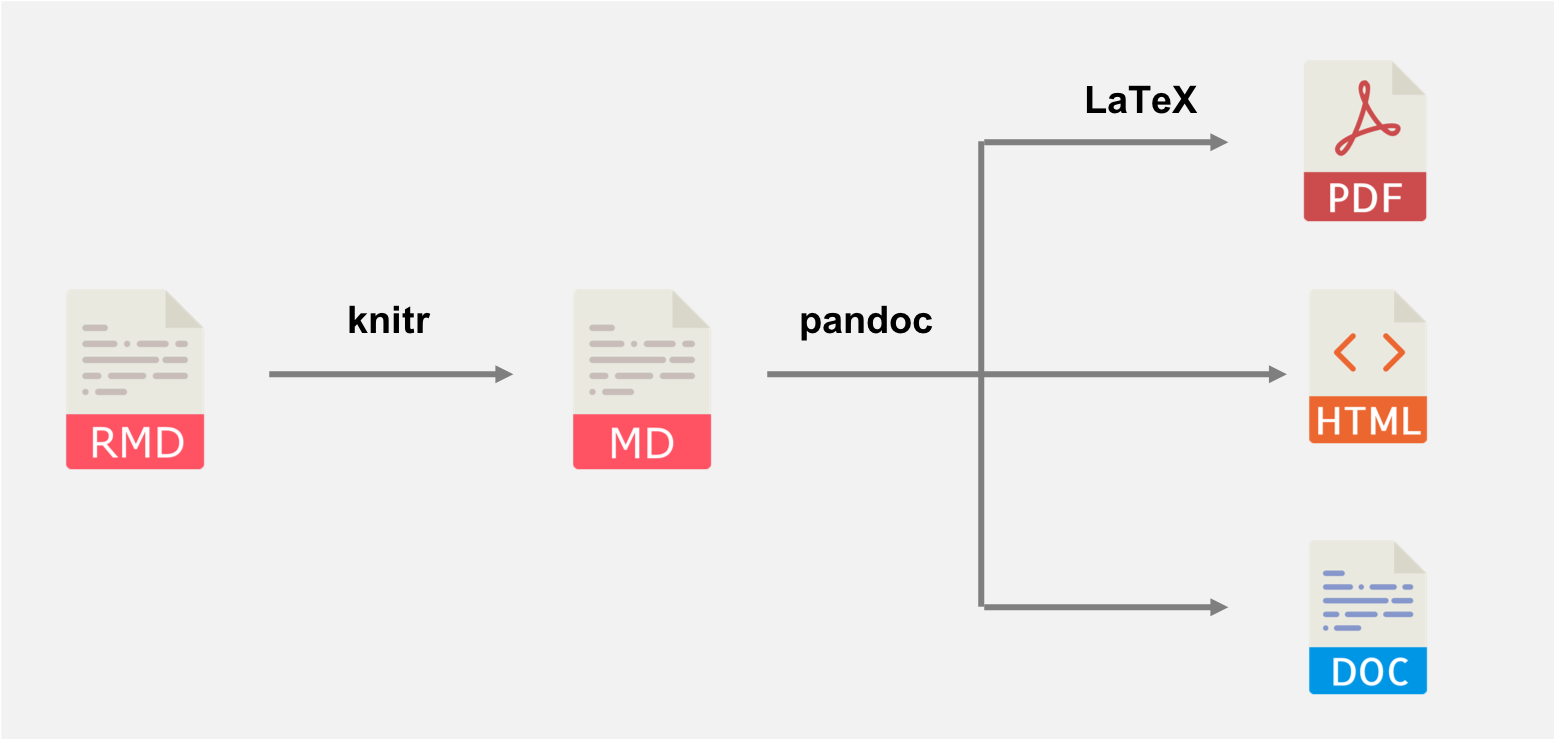
\includegraphics[width=1\linewidth,height=1\textheight,keepaspectratio]{JP/images/workflow} 

}

\caption{R Markdown 文書がどのように最終的な出力文書に変換されるかを表すダイアグラム}\label{fig:rmdworkflow}
\end{figure}

\texttt{.Rmd} 文書は, 文書の本来の形式です. YAML (メタデータ)\index{YAML}, テキスト (ナラティブ), コードチャンク\index{コードチャンク} を含んでいます.

最初に \textbf{knitr}\index{knitr} \autocite{R-knitr} の \texttt{knit()} 関数が \texttt{.Rmd} ファイルに埋め込まれた全てのコードを実行することになり, そして出力文書にコードの出力を表示します. 全ての結果は, 一時的に作られた \texttt{.md} ファイルに含まれるよう, 適正なマークアップ言語へと変換されます.

その後 \texttt{.md} ファイルは, あるマークアップ言語のファイルから別のものへと変換するための多用途なツールである Pandoc\index{Pandoc} によって処理されます. 文書を \texttt{output} パラメータで指定された (HTML へ出力する \texttt{html\_document} のような) 出力形式へ変換するため, 文書の YAML フロントマターで指定されたパラメータを取ります (例: \texttt{title}, \texttt{author}, \texttt{date}).

出力形式が PDF ならば, Pandoc が中間ファイルの \texttt{.md} を \texttt{.tex} ファイルに変換する時にさらに処理が1層, 追加されます. このファイルはその後, 最終的な PDF 文書を形成するため LaTeX によって処理されます. \ref{install-latex} 節で話したように, \textbf{rmarkdown} パッケージは \textbf{tinytex} パッケージ \textcite{R-tinytex}{]} の \texttt{latexmk()} 関数を呼び出し, これが次々に LaTeX を呼び出して \texttt{.tex} をコンパイルし \texttt{.pdf} にします.

簡潔にまとめると, \texttt{rmarkdown::render()} = \texttt{knitr::knit()} + Pandoc (PDF の場合のみ + LaTeX) ということです.

Robin Linacre が \url{https://stackoverflow.com/q/40563479/559676} で R Markdown と \textbf{knitr} と Pandoc の関係について良い要約を書いてくれました. この投稿には上記の概観よりも技術的に細かい話も含まれています.

全ての R Markdown 文書が常に Pandoc を通してコンパイルされるわけではないことに注意してください. 中間ファイル \texttt{.md} は他の Markdown レンダラによってもコンパイルできます. 例えば2つ例を挙げます.

\begin{itemize}
\item
  \textbf{xaringan}\index{xaringan} パッケージ \autocite{R-xaringan} は出力された \texttt{.md} をウェブブラウザ上で Markdown コンテンツを表示するための JavaScript ライブラリに渡します.\footnote{\textbf{訳注}: \textbf{xaringan} について日本語で言及している例は少ないですが, 次のページが用法・技術的な説明の両面で優れています. \url{https://qiita.com/nozma/items/21c56c7319e4fefceb79}}
\item
  \textbf{blogdown}\index{blogdown} パッケージは \autocite{R-blogdown} \texttt{.Rmarkdown} 文書形式をサポートしています. これは \texttt{.Rmarkdown} を knit して \texttt{.markdown} にし, Markdown 文書は大抵の場合外部のサイトジェネレータによって HTML にレンダリングされます.
\end{itemize}

\hypertarget{rmarkdown-anatomy}{%
\section{R Markdown の解剖学}\label{rmarkdown-anatomy}}

R Markdown にいくつかの部品があることを考えながら, 我々は1レベル深く掘り下げることができます. では, レンダリング作業中にいつどのように処理を変化させるかに注目してみましょう.

\hypertarget{yaml-metadata}{%
\subsection{YAML メタデータ}\label{yaml-metadata}}

YAML metadata\index{YAML} (YAML ヘッダとも呼びます) はレンダリング処理の中の多くのステージで処理され, 様々な形で最終的な文書に作用することことができます. YAML メタデータは Pandoc, \textbf{rmarkdown}, そして \textbf{knitr} のそれぞれに読み込まれます. その過程で, メタデータに含まれる情報はコード, コンテンツ, そしてレンダリング処理に影響しうるものです.

典型的な YAML ヘッダはこのように, 文書と基本的なレンダリング操作指示に関する基本的なメタデータを含んでいます.

\begin{Shaded}
\begin{Highlighting}[]
\PreprocessorTok{{-}{-}{-}}
\FunctionTok{title}\KeywordTok{:}\AttributeTok{ My R Markdown Report}
\FunctionTok{author}\KeywordTok{:}\AttributeTok{ Yihui Xie}
\FunctionTok{output}\KeywordTok{:}\AttributeTok{ html\_document}
\PreprocessorTok{{-}{-}{-}}
\end{Highlighting}
\end{Shaded}

この場合, \texttt{title}, \texttt{author} フィールドは Pandoc によって処理され, テンプレート変数の値に設定されます. デフォルトのテンプレートでは, \texttt{title} と \texttt{author} の情報は得られた文書の冒頭に現れます. Pandoc が YAML ヘッダの情報をどう扱うかのより詳細な話は, Pandoc マニュアルの \href{https://pandoc.org/MANUAL.html\#extension-yaml_metadata_block}{YAML metadata block.} に関するセクションで見られます.\footnote{\textbf{訳注}: 日本語訳での対応箇所はこちら: \url{https://pandoc-doc-ja.readthedocs.io/ja/latest/users-guide.html\#metadata-blocks}}

対照的に \texttt{output} フィールドはレンダリング処理の中で \textbf{rmarkdown} が出力フォーマット関数 \texttt{rmarkdown::html\_document()} に適用するのに使われます \texttt{output} に指定した出力フォーマットに引数をあたえることで, レンダリング処理に影響させることができます. 例えばこのように書きます.

\begin{Shaded}
\begin{Highlighting}[]
\FunctionTok{output}\KeywordTok{:}
\AttributeTok{  }\FunctionTok{html\_document}\KeywordTok{:}
\AttributeTok{    }\FunctionTok{toc}\KeywordTok{:}\AttributeTok{ }\CharTok{true}
\AttributeTok{    }\FunctionTok{toc\_float}\KeywordTok{:}\AttributeTok{ }\CharTok{true}
\end{Highlighting}
\end{Shaded}

これは \texttt{rmarkdown::render()} に, \texttt{rmarkdown::html\_document(toc = TRUE, toc\_float = TRUE)} と指示することと同じです. これらのオプションが何をするのか知るために, あるいは使える他のオプションを知るために, R コンソールで \texttt{?rmarkdown::html\_document} を実行してヘルプページを読むことになるでしょう. \texttt{output: html\_document} は \texttt{output: rmarkdown::html\_document} と等価であることに注意してください. 出力フォーマットが \texttt{rmarkdown::} のような修飾子を持たない場合, \textbf{rmarkdown} パッケージのものと想定されます. そうでないなら, R パッケージ名のプレフィックスが必要です. 例えば \texttt{bookdown::html\_document2} のような.

\ref{parameterized-reports} 節に書いたように, YAML ヘッダ内でパラメータを選択したのなら, コンテンツとコードにも影響することができます. 簡潔に言うと, R Markdown ドキュメント全体で参照可能な変数や R 評価式をヘッダに含めることができるということです. 例えば以下のヘッダでは \texttt{start\_date} と \texttt{end\_date} パラメータを定義し, これらは以降の R Markdown 文書内で \texttt{params} というリスト内に反映されます. つまり, R コード内でこれらを使うことができ, \texttt{params\$start\_date} と \texttt{params\$end\_date} でアクセスできるということです.

\begin{Shaded}
\begin{Highlighting}[]
\PreprocessorTok{{-}{-}{-}}
\FunctionTok{title}\KeywordTok{:}\AttributeTok{ My RMarkdown}
\FunctionTok{author}\KeywordTok{:}\AttributeTok{ Yihui Xie}
\FunctionTok{output}\KeywordTok{:}\AttributeTok{ html\_document}
\FunctionTok{params}\KeywordTok{:}
\AttributeTok{  }\FunctionTok{start\_date}\KeywordTok{:}\AttributeTok{ }\StringTok{\textquotesingle{}2020{-}01{-}01\textquotesingle{}}
\AttributeTok{  }\FunctionTok{end\_date}\KeywordTok{:}\AttributeTok{ }\StringTok{\textquotesingle{}2020{-}06{-}01\textquotesingle{}}
\PreprocessorTok{{-}{-}{-}}
\end{Highlighting}
\end{Shaded}

\hypertarget{narrative}{%
\subsection{ナラティブ}\label{narrative}}

ナラティブ (物語術) としてのテキスト要素は YAML メタデータやコードチャンクよりは理解が簡単でしょう. 典型的には, これはテキストエディタで書いているのと同じだと感じられるでしょう. しかし Markdown コンテンツは, どのようにコンテンツが作られるか, どうやって文書の構造がそこから作られるか, の両方に関して, 単純なテキストよりも強力で面白いものに違いありません.

世のナラティブの多くは人の手で書かれていますが, 多くの R Markdown 文書ではコードと使用される分析を参照することが求められているようです. この理由として, \ref{document-elements} 章において, コードがテキストの一部を生成するのを助ける様々な方法が実演されています. 単語を結合してリストにしたり (\ref{combine-words}節), 参考文献リストを書いたり (\ref{bibliography}節)といったやり方です. この変換は \texttt{.Rmd} から \texttt{.md} への変換と同様に \textbf{knitr}\index{knitr} で制御されます.

Markdown のテキストは文書の構造をも与えることができます. Markdown の構文をこの場で復習するには紙面が足りませんが,\footnote{Markdown の復習には, 代わりに, \url{https://bookdown.org/yihui/bookdown/markdown-syntax.html} をご覧になってください.} 特に関連深い概念の1つとしてセクション見出しがあります. これは 1つ以上の, 対応したレベルの数のハッシュ (\texttt{\#}) で表現されます. 例えば, 以下のように.

\begin{Shaded}
\begin{Highlighting}[]
\FunctionTok{\# 第1水準の見出し}

\FunctionTok{\#\# 第2水準の見出し}

\FunctionTok{\#\#\# 第3水準の見出し}
\end{Highlighting}
\end{Shaded}

これらの見出しは \textbf{rmarkdown} が \texttt{.md} を最終的な出力フォーマットに変換する際に文書全体に構造を与えます. この構造は, いくつかの属性を付与することでセクション (章や節) を参照し形成するのに役立ちます. Pandoc 構文は, 見出しの記述に \texttt{\{\#id\}} と続けることで参照を作成することが可能になり, あるいは \texttt{\{.クラス名\}} のように書くことセクションに複数のクラスを付与できます. 例えば以下のように.

\begin{Shaded}
\begin{Highlighting}[]
\FunctionTok{\#\# 第2水準の見出し \{\#introduction .important .large\}}
\end{Highlighting}
\end{Shaded}

例えば ID やクラスで参照するといった, これから学ぶいくつもの方法で, このセクションにアクセスすることができます. 具体例として, \ref{cross-ref}節ではセクションIDを使って文書内のどこでも相互参照する方法を実演していますし, \ref{html-tabs}節では小節を認識させる \texttt{.tabset} クラスを紹介しています.

R Markdown のテキスト部分で見られる最後の興味深いコンテンツのタイプとして, 特定の出力したいフォーマットに対して「生のコンテンツ」をそのまま書き出す方法, 例えば LaTeX 出力に対して LaTeX コードを直接書く (\ref{raw-latex} 節), HTML 出力に対して HTML コードを直接書く, 等 (\ref{raw-content} 節), を挙げます. 生のコンテンツは基本的な Markdown ではできないことが達成できますが, 出力フォーマットが異なるとたいていは無視されることに留意してください. 例えば生の LaTeX コマンドは出力が HTML の場合, 無視されます.

\hypertarget{code-chunks}{%
\subsection{コードチャンク}\label{code-chunks}}

コードチャンク\index{code chunk}は R Markdown にとっての心臓の鼓動です. チャンク内のコードは \textbf{knitr} によって実行され, 出力は Markdown に翻訳され, レポートは現在のスクリプトとデータに動的に同期します. 各コードチャンクは言語エンジン (\ref{other-languages}章), ラベル, チャンクオプション (\ref{chunk-options}章), そしてコードで構成されます.

コードチャンクを作ることができるいくつかの mod について理解するためには, \textbf{knitr} の処理をあとほんの少しだけ詳しく知ることが有意義です. 各チャンクでは, \textbf{knitr} 言語エンジンは3つの入力の部品を得ます. knit 環境 (\texttt{knitr::knit\_global()}), コードの入力, 任意に指定できるラベル, そしてチャンクオプションのリストです. コードチャンクはコードもその出力も整形された表現として返します. 副作用として, knit 環境も修正されます. 例えばコードチャンク内のソースコードを介してこの環境内で新しい変数がつくられます. この処理は図\ref{fig:knitr-workflow}のように表せます.

\begin{figure}

{\centering \includegraphics[width=1\linewidth,height=1\textheight,keepaspectratio]{rmarkdown-cookbook_files/figure-latex/knitr-workflow-1} 

}

\caption{言語エンジンへの入出力フローチャート}\label{fig:knitr-workflow}
\end{figure}

この処理は以下の方法で修正できます.

\begin{itemize}
\item
  言語エンジンを変更する
\item
  チャンクオプションを, グローバルあるいはローカル, あるいは特定の言語に対してのみ修正する
\item
  入出力にさらなる処理を追加するためのフックを使用する
\end{itemize}

例えば\ref{hook-hide}節で, ソースコードの特定行を改ざんする後処理をするフックを加える方法を学ぶことになるでしょう.

コードチャンクは\ref{narrative}節でつぶさに見てきたナラティブのようなクラスと識別子を持ちます. コードチャンクは識別子 (よく「チャンクラベル」と呼ばれます) を言語エンジンの直後に任意で指定することができます. チャンクオプション \texttt{class.source} と \texttt{class.output} でそれぞれコードブロックとテキスト出力ブロックに対するクラスを設定することもできます (\ref{chunk-styling}節参照). 例えばチャンクヘッダ \texttt{\textasciigrave{}\textasciigrave{}\textasciigrave{}\{r\ summary-stats,\ class.output\ =\ \textquotesingle{}large-text\textquotesingle{}\}} はチャンクラベルに \texttt{summary-stats} を与え, テキスト出力ブロックに \texttt{large-text} というクラスを与えています. チャンクのラベルは1つだけですが, クラスは複数持つことができます.

\hypertarget{document-body}{%
\subsection{文書の本文}\label{document-body}}

文書を執筆し編集するに際して理解すべき重要なことは, どのようにしてコードとナラティブの小片が文書内のいくつもの節やコンテナを作るのかです. 例えばこのような文書があったとします.

\begin{Shaded}
\begin{Highlighting}[]
\FunctionTok{\# タイトル}

\FunctionTok{\#\# X 節}

\NormalTok{ここから導入文}

\InformationTok{\textasciigrave{}\textasciigrave{}\textasciigrave{}\{r chunk{-}x\}}
\InformationTok{x \textless{}{-} 1}
\InformationTok{print(x)}
\InformationTok{\textasciigrave{}\textasciigrave{}\textasciigrave{}}

\FunctionTok{\#\#\# 第1小節}

\NormalTok{ここに詳細な話}

\FunctionTok{\#\#\# 第2小節}

\NormalTok{ここにさらに詳しい話}

\FunctionTok{\#\# Y 節}

\NormalTok{ここから新しい節}

\InformationTok{\textasciigrave{}\textasciigrave{}\textasciigrave{}\{r chunk{-}y\}}
\InformationTok{y \textless{}{-} 2}
\InformationTok{print(y)}
\InformationTok{\textasciigrave{}\textasciigrave{}\textasciigrave{}}
\end{Highlighting}
\end{Shaded}

この文書を書いていると, それぞれの小片は, テキストとコードを含んだ, 独立した節とともに直線上に並んでいるものとみなすかもしれません. しかし実際にしているのは, 概念としては図\ref{fig:rmd-containers}でより細かく描いているように, 入れ子 (ネスト) になったコンテナの作成です\footnote{現実に, ここで見えているよりも多くのコンテナがあります. 例えば knit されたコードチャンクや, コードと出力がそれぞれ別のコンテナとして存在し, そしてこれらは親要素を共有しています.}

\begin{figure}

{\centering \includegraphics[width=0.5\linewidth,height=1\textheight,keepaspectratio]{rmarkdown-cookbook_files/figure-latex/rmd-containers-1} 

}

\caption{入れ子状のコンテナとして表現された単純な R Markdown 文書の例}\label{fig:rmd-containers}
\end{figure}

この図に関する2つの重要な特徴は (1) テキストやコードのどのセクションも個別のコンテナであり, (2) コンテナは他の別のコンテナを入れ子にできる, ということです. この入れ子は R Markdown 文書を RStudio IDE で執筆し, 文書のアウトラインを展開しているとはっきりと分かります.

図\ref{fig:rmd-containers}では同じレベルのヘッダは同じレベルの入れ子を表していることに注意してください. 低レベルのヘッダはより高レベルなヘッダのコンテナ内部にあります. この場合, 通常は高レベルの節を「親」といい, 低レベルの節を「子」といいます. 例えば「小節」は「節」の子です. \ref{multi-column}節で実演するように, ヘッダだけでなく \texttt{:::} を使ってまとまりの単位を作ることができます

このテキストで説明されているフォーマットやスタイルのオプションを適用するとき, この構造は重要な意味を持ちます. 例えば, Pandoc が抽象構文木 (AST) でどのように文書を表現するかを学ぶ時 (\ref{lua-filters}節) や, HTML出力のスタイルを決めるために CSS セレクタを使用する時 (\ref{html-css}節ほか), 入れ子構造の概念が現れます.

フォーマットとスタイルは似たようなタイプのコンテナ (例えばコードブロック) や, あるコンテナ内に全てあるコンテナ (例: 「Y 節」以下にある全てのコンテナ) に対して適用できます. 加えて\ref{narrative}節で説明したように, 同一のクラスをある節に対して同様のものとして扱うために適用することができますし, この場合は共通のクラス名は共通のプロパティ, あるいはこの節に共通の意図を示すようになります.

本書を読みながら, 特定の「レシピ」がどんな種類のコンテナに対して作用しているのかを自問し, 考えることはあなたにとって有益になるでしょう.

\hypertarget{what-to-change}{%
\section{結果を変えるために変更できるのはなにか?}\label{what-to-change}}

では, ここまでで概観してきたものを要約し, これから何をすべきかを下見していきましょう.

\textbf{rmarkdown} で R Markdown 文書をレンダリングする処理は \textbf{knitr} で \texttt{.Rmd} を \texttt{.md} で変換する処理, それから (典型的には) Pandoc で \texttt{.md} を望む出力に変換する処理で構成されます.

\texttt{.Rmd} から \texttt{.md} 変換のステップではレポート内の全てのコードの実行と「翻訳」を制御するため, 「コンテンツ」への変更のほとんどは, \textbf{knitr} の翻訳するためのコードを伴う \texttt{.Rmd} を編集する作業が絡んできます. これらのステップ全体を操作するツールには \textbf{knitr} チャンクオプションおよびフックがあります.

\texttt{.md} はフォーマットされていないプレーンテキストです. ここで Pandoc の出番です. HTML や PDF, Word といった最終的な出力フォーマットへ変換されます. この途上で構造とスタイルを付与します. この処理では スタイルシート (CSS), 生 LaTeX または HTML コード, Pandoc テンプレート, Lua フィルタといった様々なツールが助けになります. R Markdown 文書の入れ子構造を理解し, よく考えて識別子とクラスを使うことで, これらのツールを取捨選択して出力の目標となる箇所に応用することができます.

最後に, YAML メタデータはこれらのステップの切り替えに役に立つかも知れません. パラメータの変更はコードがどう動作するかを変更することができ, メタデータの変更はテキストの内容を変化させ, 出力オプションの変更は, 異なる命令のセットをもつ \texttt{render()} 関数を与えます.

もちろんこれらは全て大まかな経験則であり, 絶対的な事実として扱うべきでありません. 究極的には, 機能を完璧にきれいに分類することはできません. 本書全体を通じて, 説明されている結果の多くは, しばしば実現のための道筋が複数あり, さらにそのパイプラインの様々なステージの説明に立ち入ることになることが分かるでしょう. 例えば文書内に画像を挿入する作業では, \texttt{.Rmd} から \texttt{.md} への変換の段階で R コード \texttt{knitr::include\_graphics()} を使うこともあれば, Markdown 構文 (\texttt{!{[}{]}()}) を直接使うこともあるでしょう. ややこしく思えるかもしれませんし, アプローチごとに異なる利点を持つこともあります. しかし悩まないでください. なんにせよ, あなたの問題を解決する多くの有効な方法が存在し, あなたはそれらから自分にとって最も理にかなうアプローチに従うことができます.

さあこの辺にしておきましょう. 本書の残りの部分で, R Markdown を最大限活用するために我々が説明した, あらゆるコンポネントを変更する方法のより具体的な例を使って, あなたの絵の下書きに色をつけることができます.

\hypertarget{basics}{%
\chapter{基本}\label{basics}}

この章では, R Markdown の重要な概念をいくつか提示します. まず「平文」「コード」という R Markdown の基本的なコンポネントを紹介します. 次に, R Markdown 文書をどう R スクリプトへ変換するか, あるいは逆はどうするかを提示します.

もっと基本的な話を求める方は, \emph{R Markdown Definitive Guide} \autocite{rmarkdown2018} の2章を見てください.

\hypertarget{r-code}{%
\section{コードチャンクとインライン R コード}\label{r-code}}

R Markdown 文書は平文 (ナラティブ) とコードが混合してできています. Rmd 文書には2種類のコード, コードチャンク\index{コードチャンク}とインライン (行内) R コードです. 以下は簡単な例です.

\begin{Shaded}
\begin{Highlighting}[]
\InformationTok{\textasciigrave{}\textasciigrave{}\textasciigrave{}\{r\}}
\InformationTok{x \textless{}{-} 5  \# 円の半径}
\InformationTok{\textasciigrave{}\textasciigrave{}\textasciigrave{}}

\NormalTok{半径 }\InformationTok{\textasciigrave{}r x\textasciigrave{}}\NormalTok{ の円に対し,}
\NormalTok{その面積は }\InformationTok{\textasciigrave{}r pi * x\^{}2\textasciigrave{}}\NormalTok{ である.}
\end{Highlighting}
\end{Shaded}

コードチャンクはたいていは \texttt{\textasciigrave{}\textasciigrave{}\textasciigrave{}\{\}} で始まり, \texttt{\textasciigrave{}\textasciigrave{}\textasciigrave{}} で終わります. コードチャンク内ではコードを何行でも書いてかまいません. インライン R コードは \texttt{\textasciigrave{}r\ \textasciigrave{}} という構文を使って文書のナラティブの中に埋め込まれます. 上記の例ではコードチャンク内で円の半径として変数 \texttt{x} を定義し, この円の面積を次のパラグラフで計算しています.

チャンクオプションを通してコードチャンクの挙動と出力をカスタマイズできます (オプションはカーリー・ブレイス \texttt{\{\}} 内に与えます). 例のいくつかは\ref{chunk-options}章で見つかるでしょう. コードチャンクに別のプログラミング言語のコードを書くこともあるでしょう (\ref{other-languages} 章を見てください).

\hypertarget{rstudio-visual}{%
\section{RStudio のビジュアルエディタで R Markdown を書く}\label{rstudio-visual}}

あなたがまだ Markdown の書き方に慣れていないか, Markdown コードを書くのが気に入らないならば, RStudio\index{RStudio} ver. 1.4 には実験的ですが Markdown 文書用のビジュアルエディタがあります. これは図\ref{fig:visual-edit}で示すように Word のような伝統的な WYSIWYG なエディタと似ていると感じるでしょう. この完全なドキュメントは \url{https://rstudio.github.io/visual-markdown-editing/} で見ることができます.

\begin{figure}

{\centering 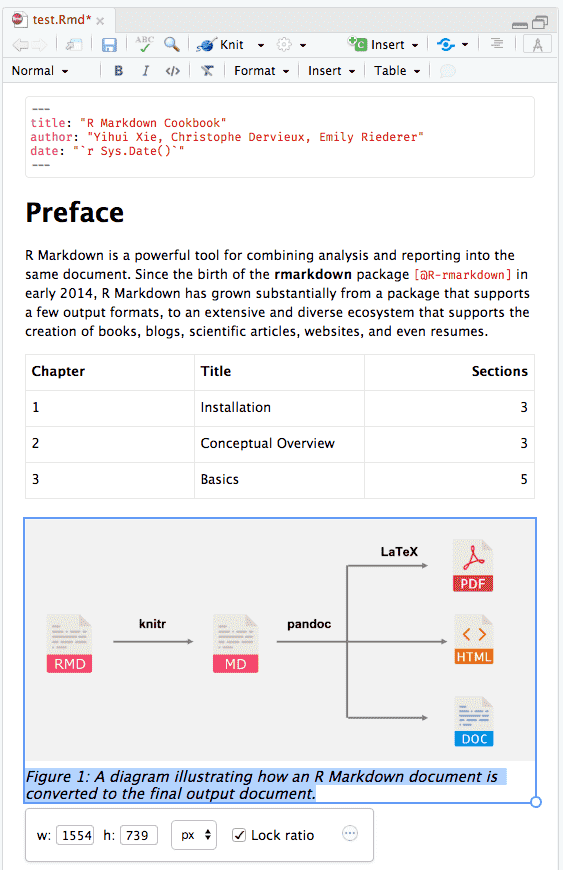
\includegraphics[width=1\linewidth,height=1\textheight,keepaspectratio]{JP/images/visual-edit} 

}

\caption{RStudio のビジュアル Markdown エディタ}\label{fig:visual-edit}
\end{figure}

ビジュアルエディタによって, ヘッダ, 図, 表, 脚注などといった Pandoc でサポートされているほとんどあらゆる Markdown 要素を視覚的に編集できます. あなたは全ての構文を覚えなくてもよいということです. ある要素の構文を忘れた場合, RStudio ツールバー (図\ref{fig:visual-edit}参照) を使うかキーボードショートカットを使って要素を追加したり編集したりすることになるでしょう.

あなたが既に Markdown に熟練しているなら, ツールバーを右クリックしてソースモードとビジュアルモードを切り替えられるので, 文書をソースモードのままで書くこともできます.

\hypertarget{spin}{%
\section{R スクリプトをレポートにレンダリングする}\label{spin}}

年季の入った Rを Markdown ユーザーであっても, 別の選択肢があることを見落としているかもしれません. Dean Attali はこれを\href{https://deanattali.com/2015/03/24/knitrs-best-hidden-gem-spin/}{"\textbf{knitr} の隠された至宝}と読んでいます. 純粋な R スクリプトを直接レンダリングできるということです. RStudio IDE をお使いなら, R スクリプトをレンダリングするキーボードショートカットは Rmd 文書を knit するとき (\texttt{Ctrl / Cmd + Shift + K}) と同じです.

R スクリプトをレポートにレンダリングすると, まず \texttt{knitr::spin()}\index{knitr!spin()} 関数が呼ばれスクリプトが Rmd ファイルに変換されます. この関数が Dean Attali が「\textbf{knitr}の隠された至宝」と呼んでいるものです. レポートには全てのテキストとグラフィックの出力が掲載されます.

レポートの要素を細かく管理したいなら, 以下のようにその助けとなるいくつかの構文があります.

\begin{itemize}
\item
  Roxygen コメントは平文として扱われます. roxygen コメントは \texttt{\#\textquotesingle{}} で始まる R コメントで, レポートにナラティブを書くのに役立つかもしれません. コメント内ではあらゆる Markdown 構文を使うことができます.
\item
  \texttt{\#+} で始まるコメントは \texttt{knitr} チャンクヘッダとして扱われます. 例えば \texttt{\#+ label, fig.width=5} というコメントを, \texttt{knitr::spin()} は R Markdown の \texttt{\textasciigrave{}\textasciigrave{}\textasciigrave{}\{r\ label,\ fig.width=5\}} というチャンクヘッダへ翻訳します.
\item
  \texttt{\{\{ code \}\}} で囲まれた R コードは R Markdown のインライン R コードへ翻訳されます. \texttt{\{\{ code \}\}} は1行で書かなければならないことに注意してください.
\item
  YAML\index{YAML} フロントマターも, R スクリプトの冒頭の roxigen コメント内に書くことができます. YAML フィールドのインデントによく気をつけてください. YAML のインデントを省くとデータ構造の表現は不正確なものに変わることがあります. 例えば \texttt{keep\_tex: true} というフィールドは, 後述する例のように \texttt{pdf\_document} 以下に2つ以上のスペースでインデントするべきです.
\item
  \texttt{/*} と \texttt{*/} の間の任意のテキストは無視されます (つまり, 完全にコメントとして扱われます)
\end{itemize}

上記のルールの全ての例を表現したのが以下です.

\begin{Shaded}
\begin{Highlighting}[]
\CommentTok{\#\textquotesingle{} {-}{-}{-}}
\CommentTok{\#\textquotesingle{} title: "純粋な R script から生成したレポート"}
\CommentTok{\#\textquotesingle{} output:}
\CommentTok{\#\textquotesingle{}   pdf\_document:}
\CommentTok{\#\textquotesingle{}     keep\_tex: true}
\CommentTok{\#\textquotesingle{} {-}{-}{-}}
\CommentTok{\#\textquotesingle{}}
\CommentTok{\#\textquotesingle{} これは \textasciigrave{}knitr::spin()\textasciigrave{} によって生成されたレポートです.}
\CommentTok{\#\textquotesingle{}}
\CommentTok{\#\textquotesingle{} **knitr** オプションをいくつか試してみましょう:}

\CommentTok{\#+ echo=FALSE, fig.width=7}
\CommentTok{\#  これは通常の R コメント文です.}
\FunctionTok{plot}\NormalTok{(cars)}

\CommentTok{\#\textquotesingle{} ここにインラインの値を書きましょう. $\textbackslash{}pi$ の値は}
\NormalTok{\{\{ pi \}\}}
\CommentTok{\#\textquotesingle{} であると知られています.}
\CommentTok{\#\textquotesingle{}}
\CommentTok{\#\textquotesingle{} 最後に, 全ての roxygen コメントは任意だということを書いておきます.}
\CommentTok{\#\textquotesingle{} プロットの大きさなど出力要素をコントロールしようと思わない限り}
\CommentTok{\#\textquotesingle{} チャンクオプションも必要でありません}

\CommentTok{\# /* C 言語のコメントのように /* と */ の間にコメントを書きましょう:}
\FunctionTok{Sys.sleep}\NormalTok{(}\DecValTok{60}\NormalTok{)}
\CommentTok{\# */}
\end{Highlighting}
\end{Shaded}

このスクリプトがレポートにレンダリングされた時, \texttt{knitr::spin()} はこれを R Markdown へと変換します.

\begin{Shaded}
\begin{Highlighting}[]
\CommentTok{{-}{-}{-}}
\AnnotationTok{title:}\CommentTok{ "純粋な R script から生成したレポート"}
\AnnotationTok{output:}
\CommentTok{  pdf\_document:}
\CommentTok{    keep\_tex: true}
\CommentTok{{-}{-}{-}}

\NormalTok{これは }\InformationTok{\textasciigrave{}knitr::spin()\textasciigrave{}}\NormalTok{ によって生成されたレポートです.}

\NormalTok{**knitr** オプションをいくつか試してみましょう:}

\InformationTok{\textasciigrave{}\textasciigrave{}\textasciigrave{}\{r echo=FALSE, fig.width=7\}}
\InformationTok{\#  これは通常の R コメント文です.}
\InformationTok{plot(cars)}
\InformationTok{\textasciigrave{}\textasciigrave{}\textasciigrave{}}

\NormalTok{ここにインラインの値を書きましょう. $\textbackslash{}pi$ の値は}
\InformationTok{\textasciigrave{}\textasciigrave{}r  pi  \textasciigrave{}\textasciigrave{}}
\NormalTok{であると知られています.}

\NormalTok{最後に, 全ての roxygen コメントは任意だということを書いておきます.}
\NormalTok{プロットの大きさなど出力要素をコントロールしようと思わない限り}
\NormalTok{チャンクオプションも必要でありません}
\end{Highlighting}
\end{Shaded}

このレポート生成方法は, 主に R スクリプトを使って作業していて, 多くのナラティブを必要としないときに特に役立つかもしれません. レポートが実質テキストであるほどの割合のテキストなら, 全てのテキストを roxygen コメントに入れなくてもいいので R Markdown がより良い選択かもしれません.

\hypertarget{purl}{%
\section{Markdown から R script への変換}\label{purl}}

R Markdown から全ての R コードを取り出したい時, あなたは \texttt{knitr::purl()}\index{knitr!purl()} を呼ぶことができます. 以下は \texttt{purl.Rmd} というファイル名の簡単な Rmd の例です.

\begin{Shaded}
\begin{Highlighting}[]
\CommentTok{{-}{-}{-}}
\AnnotationTok{title:}\CommentTok{ R コードを取りだすために \textasciigrave{}purl()\textasciigrave{} を使いましょう}
\CommentTok{{-}{-}{-}}

\InformationTok{\textasciigrave{}knitr::purl()\textasciigrave{}}\NormalTok{ 関数は **knitr** 文書から  R コードチャンクを取り出しコードを R スクリプトに保存します.}

\NormalTok{以下は簡単なチャンクです.}

\InformationTok{\textasciigrave{}\textasciigrave{}\textasciigrave{}\{r, simple, echo=TRUE\}}
\InformationTok{1 + 1}
\InformationTok{\textasciigrave{}\textasciigrave{}\textasciigrave{}}

\InformationTok{\textasciigrave{}r 2 * pi\textasciigrave{}}\NormalTok{ のようなインライン R 式はデフォルトでは無視されます.}

\NormalTok{特定のコードチャンクを取り出してほしくない場合は, チャンクオプション }\InformationTok{\textasciigrave{}purl = FALSE\textasciigrave{}}\NormalTok{ を設定できます. 例えば以下のように.}

\InformationTok{\textasciigrave{}\textasciigrave{}\textasciigrave{}\{r, ignored, purl=FALSE\}}
\InformationTok{x = rnorm(1000)}
\InformationTok{\textasciigrave{}\textasciigrave{}\textasciigrave{}}
\end{Highlighting}
\end{Shaded}

\texttt{knitr::purl("purl.Rmd")} を呼び出したら, 以下の R スクリプト (デフォルトのファイル名は \texttt{purl.R}) が生成されます.

\begin{Shaded}
\begin{Highlighting}[]
\DocumentationTok{\#\# {-}{-}{-}{-} simple, echo=TRUE{-}{-}{-}{-}{-}{-}{-}{-}{-}{-}{-}{-}{-}{-}{-}{-}{-}{-}{-}{-}{-}{-}{-}{-}{-}{-}{-}{-}{-}{-}}
\DecValTok{1} \SpecialCharTok{+} \DecValTok{1}
\end{Highlighting}
\end{Shaded}

上記の R スクリプトでは, チャンクオプションはコメントとして書かれています. 純粋な R コードが欲しい場合, \texttt{documentation = 0} という引数を与えて \texttt{knitr::purl()} を呼ぶことになるでしょう. これで以下のような R スクリプトが生成されます.

\begin{Shaded}
\begin{Highlighting}[]
\DecValTok{1} \SpecialCharTok{+} \DecValTok{1}
\end{Highlighting}
\end{Shaded}

テキストも全て維持したい場合 \texttt{documentation = 2} 引数を使うことになるでしょう. これは以下のような R スクリプトを生成します.

\begin{Shaded}
\begin{Highlighting}[]
\CommentTok{\#\textquotesingle{} {-}{-}{-}}
\CommentTok{\#\textquotesingle{} title: R コードを取りだすために \textasciigrave{}purl()\textasciigrave{} を使いましょう}
\CommentTok{\#\textquotesingle{} {-}{-}{-}}
\CommentTok{\#\textquotesingle{} }
\CommentTok{\#\textquotesingle{} \textasciigrave{}knitr::purl()\textasciigrave{} 関数は **knitr** 文書から  R コードチャンクを取り出しコードを R スクリプトに保存します.}
\CommentTok{\#\textquotesingle{} }
\CommentTok{\#\textquotesingle{} 以下は簡単なチャンクです.}
\CommentTok{\#\textquotesingle{} }
\DocumentationTok{\#\# {-}{-}{-}{-} simple, echo=TRUE{-}{-}{-}{-}{-}{-}{-}{-}{-}{-}{-}{-}{-}{-}{-}{-}{-}{-}{-}{-}{-}{-}{-}{-}{-}{-}{-}{-}{-}{-}}
\DecValTok{1} \SpecialCharTok{+} \DecValTok{1}

\CommentTok{\#\textquotesingle{} }
\CommentTok{\#\textquotesingle{} \textasciigrave{}r 2 * pi\textasciigrave{} のようなインライン R 式はデフォルトでは無視されます.}
\CommentTok{\#\textquotesingle{} }
\CommentTok{\#\textquotesingle{} 特定のコードチャンクを取り出してほしくない場合は, チャンクオプション \textasciigrave{}purl = FALSE\textasciigrave{} を設定できます. 例えば以下のように.}
\CommentTok{\#\textquotesingle{} }
\end{Highlighting}
\end{Shaded}

\texttt{purl = FALSE} というオプションのあるコードチャンクはこの R スクリプトから除外されることに注意してください.

インライン R コードはデフォルトでは無視されます. R スクリプトにインライン表現も含めたいなら, \texttt{knitr::purl()} を呼ぶ前に R のグローバルオプション \texttt{options(knitr.purl.inline = TRUE)} を設定する必要があります.

\hypertarget{notebook}{%
\section{R Markdown Notebook}\label{notebook}}

\emph{R Markdown Definitive Guide} \autocite{rmarkdown2018} の \href{https://bookdown.org/yihui/rmarkdown/compile.html}{Section 2.2} で言及したように, Rmd 文書をコンパイルする方法はいくつかあります. その1つは \texttt{html\_notebook} という出力形式で R Markdown Notebook を使うことです. 例えば以下のように.

\begin{Shaded}
\begin{Highlighting}[]
\PreprocessorTok{{-}{-}{-}}
\FunctionTok{title}\KeywordTok{:}\AttributeTok{ An R Markdown Notebook}
\FunctionTok{output}\KeywordTok{:}\AttributeTok{ html\_notebook}
\PreprocessorTok{{-}{-}{-}}
\end{Highlighting}
\end{Shaded}

RStudio でこの出力形式を使うと, ツールバー上の \texttt{knit} ボタンが \texttt{Preview} ボタンになります.

notebook\index{RStudio!notebook} を使う主な利点は Rmd 文書を\textbf{同じRセッションで繰り返し}作業できることです. コードチャンクにある緑色の矢印ボタンを押すことでチャンクを個別に随時実行し, エディタ上でテキストやグラフの出力を見ることができます. ツールバー上の \texttt{Preview} ボタンを押せば Rmd 文書は, あなたが既に実行したコードチャンクの出力を含む HTML 出力の文書へのみレンダリングされます. \texttt{Preview} ボタンは一切のコードチャンクを実行しません. これと比較して, 他の出力形式を使い \texttt{knit} ボタンを押せば RStudio は文書全体をコンパイルする (つまり全てのコードチャンクが一気に実行されます) ために R セッションを新規で立ち上げます. これはたいてい, より時間がかかります.

コードチャンクを個別に実行した時に出力が表示されるという RStudio のデフォルトの挙動が気に入らないなら, \texttt{Tools -\textgreater{}\ Global\ Options\ -\textgreater{}\ R\ Markdown} から ``Show output inline for all R Markdown documents'' というオプションのチェックを外すことができます. 以降は, コードチャンクを実行すると出力はソースエディタ内ではなく R コンソールに表示されます. このオプションは YAML メタデータで個別の Rmd 文書ごとに設定できます. このように.

\begin{Shaded}
\begin{Highlighting}[]
\FunctionTok{editor\_options}\KeywordTok{:}
\AttributeTok{  }\FunctionTok{chunk\_output\_type}\KeywordTok{:}\AttributeTok{ console}
\end{Highlighting}
\end{Shaded}

\hypertarget{document-elements}{%
\chapter{文書の要素}\label{document-elements}}

本章では, 改ページ, YAML メタデータ, セクションヘッダ, 引用, 相互参照, 数式, アニメーション, 対話的プロット, ダイアグラム, コメントといった R Markdown 文書の要素をカスタマイズしたり生成したりするのに使える豆知識と小ワザを紹介します.

\hypertarget{pagebreaks}{%
\section{改ページ (改段) を挿入する}\label{pagebreaks}}

改ページしたい場合\index{改行}, \texttt{\textbackslash{}newpage} を文書に挿入できます.\footnote{\textbf{訳注}: 正確には \texttt{\textbackslash{}newpage} コマンドは改「段」です. 二段組の場合, 次の段に改めるため, 必ずページを改めるわけではありません.} これは LaTeX コマンドですが, \textbf{rmarkdown} パッケージは LaTeX 出力フォーマットでも, HTML, Word, ODT などのいくつかの非 LaTeX 出力フォーマットでも認識することができます.\footnote{HTML 出力では, 改ページは HTML ページの出力時のみ意味をなし, それ以外では HTML は単一の連続したページになるため, 改ページを見ることはありません.}

例えば以下のように.

\begin{Shaded}
\begin{Highlighting}[]
\CommentTok{{-}{-}{-}}
\AnnotationTok{title:}\CommentTok{ Breaking pages}
\AnnotationTok{output:}
\CommentTok{  pdf\_document: default}
\CommentTok{  word\_document: default}
\CommentTok{  html\_document: default}
\CommentTok{  odt\_document: default}
\CommentTok{{-}{-}{-}}

\FunctionTok{\# 第一節}

\NormalTok{\textbackslash{}newpage}

\FunctionTok{\# 第二節}
\end{Highlighting}
\end{Shaded}

これは Pandoc の Lua フィルタ\index{Lua フィルタ} に基づく機能です (\ref{lua-filters} 節参照). 技術的なことに興味のある方はこのパッケージの vignettte を見てください.

\begin{Shaded}
\begin{Highlighting}[]
\FunctionTok{vignette}\NormalTok{(}\StringTok{"lua{-}filters"}\NormalTok{, }\AttributeTok{package =} \StringTok{"rmarkdown"}\NormalTok{)}
\end{Highlighting}
\end{Shaded}

\hypertarget{dynamic-yaml}{%
\section{文書タイトルを動的に設定する}\label{dynamic-yaml}}

Rmd 文書内のどこでも, YAML メタデータの部分であってもインライン R コード (\ref{r-code}節) を使うことができます. つまりインライン R コードによって文書のタイトルなどの YAML メタデータの動的生成\index{YAML!動的生成}が可能ということです. 例えばこのように.

\begin{Shaded}
\begin{Highlighting}[]
\PreprocessorTok{{-}{-}{-}}
\FunctionTok{title}\KeywordTok{:}\AttributeTok{ }\StringTok{"自動車 \textasciigrave{}r nrow(mtcars)\textasciigrave{} 台の分析"}
\PreprocessorTok{{-}{-}{-}}
\end{Highlighting}
\end{Shaded}

タイトルが以降の文書内で作成される R の変数に依存する場合, 以下の例のようにその後に YAML セクションを書いて \texttt{title} フィールドを加えることになるでしょう.

\begin{Shaded}
\begin{Highlighting}[]
\CommentTok{{-}{-}{-}}
\AnnotationTok{author:}\CommentTok{ "利口なアナリスト"}
\AnnotationTok{output:}\CommentTok{ pdf\_document}
\CommentTok{{-}{-}{-}}

\NormalTok{我々の市場シェアを頑張って計算してみました.}
\NormalTok{I just tried really hard to calculate our market share:}

\InformationTok{\textasciigrave{}\textasciigrave{}\textasciigrave{}\{r\}}
\InformationTok{share \textless{}{-} runif(1)}
\InformationTok{\textasciigrave{}\textasciigrave{}\textasciigrave{}}

\NormalTok{{-}{-}{-}}
\NormalTok{title: "我々の市場シェアは今や }\InformationTok{\textasciigrave{}r round(100 * share, 2)\textasciigrave{}}\NormalTok{\% です!"}
\NormalTok{{-}{-}{-}}

\NormalTok{これはとても }\InformationTok{\textasciigrave{}r if(share \textgreater{} 0.8) "喜ばしい" else "悲しい"\textasciigrave{}}\NormalTok{ ことです.}
\end{Highlighting}
\end{Shaded}

上記の例では, 変数 \texttt{share} を作成してから文書のタイトルを追加しています. Pandoc は文書内に YAML セクションをいくつ書いても読み込む (そして全てマージする) ことができるため, この例が動作します.

タイトルだけでなくどの YAML フィールドも, パラメータ化されたレポート\index{YAML!パラメータ|see {パラメータ}}\index{パラメータ}から動的に生成することができます (\ref{parameterized-reports} 節参照). 例えばこのように.

\begin{Shaded}
\begin{Highlighting}[]
\PreprocessorTok{{-}{-}{-}}
\FunctionTok{title}\KeywordTok{:}\AttributeTok{ }\StringTok{"\textasciigrave{}r params$doc\_title\textasciigrave{}"}
\FunctionTok{author}\KeywordTok{:}\AttributeTok{ }\StringTok{"利口なアナリスト"}
\FunctionTok{params}\KeywordTok{:}
\AttributeTok{  }\FunctionTok{doc\_title}\KeywordTok{:}\AttributeTok{ }\StringTok{"デフォルトのタイトル"}
\PreprocessorTok{{-}{-}{-}}
\end{Highlighting}
\end{Shaded}

タイトルが動的なパラメータなら, タイトルだけ異なるレポートのまとまりを簡単に生成できます.

この節ではタイトルを例にしましたが, このアイディアは YAML セクションのどのメタデータのフィールドにも適用可能です.

\hypertarget{document-metadata}{%
\section{R コード内で文書メタデータにアクセスする}\label{document-metadata}}

Rmd 文書をコンパイルする際に, YAML セクション\index{YAML}の全てのメタデータはリストオブジェクト \texttt{rmarkdown::metadata} に保存されます. 例えば \texttt{rmarkdown::metadata\$title} は文書のタイトルを与えます. YAML メタデータに与えられた情報をハードコードしなくてすむように, この \texttt{metadata} オブジェクトを R コード内で使うことができます. 例えば \textbf{blastula} パッケージ \autocite{R-blastula}\index{R パッケージ!blastula} で Eメールを送る時, 文書のタイトルをメールの件名に, 著者フィールドを送信者情報に使うことができます.

\begin{Shaded}
\begin{Highlighting}[]
\CommentTok{{-}{-}{-}}
\AnnotationTok{title:}\CommentTok{ 重要なレポート}
\AnnotationTok{author:}\CommentTok{ John Doe}
\AnnotationTok{email:}\CommentTok{ john@example.com}
\CommentTok{{-}{-}{-}}

\NormalTok{重要な分析ができましたので結果をメールで送りたいと思います.}

\InformationTok{\textasciigrave{}\textasciigrave{}\textasciigrave{}\{r\}}
\InformationTok{library(rmarkdown)}
\InformationTok{library(blastula)}
\InformationTok{smtp\_send(}
\InformationTok{  ...,}
\InformationTok{  from = setNames(metadata$email, metadata$author),}
\InformationTok{  subject = metadata$title}
\InformationTok{)}
\InformationTok{\textasciigrave{}\textasciigrave{}\textasciigrave{}}
\end{Highlighting}
\end{Shaded}

\hypertarget{unnumbered-sections}{%
\section{番号のない節}\label{unnumbered-sections}}

ほとんどの出力フォーマットは \texttt{number\_sections}\index{出力オプション!number\_sections} オプションをサポートしています. これは \texttt{true} を設定すれば節への付番を有効にできるオプションです. 例えば以下のように.

\begin{Shaded}
\begin{Highlighting}[]
\FunctionTok{output}\KeywordTok{:}
\AttributeTok{  }\FunctionTok{html\_document}\KeywordTok{:}
\AttributeTok{    }\FunctionTok{number\_sections}\KeywordTok{:}\AttributeTok{ }\CharTok{true}
\AttributeTok{  }\FunctionTok{pdf\_document}\KeywordTok{:}
\AttributeTok{    }\FunctionTok{number\_sections}\KeywordTok{:}\AttributeTok{ }\CharTok{true}
\end{Highlighting}
\end{Shaded}

特定の節に番号を付けたくないならば, \texttt{number\_sections} オプションは \texttt{true} のままにして, その節のヘッダの直後に \texttt{\{-\}} を加えます. 例えばこのように.

\begin{Shaded}
\begin{Highlighting}[]
\FunctionTok{\# この節には番号がつきません \{{-}\}}
\end{Highlighting}
\end{Shaded}

全く同じことを, \texttt{\{.unnumbered\}} を使ってもできます. 例えば \texttt{\{.unnumbered \#section-id\}} のように, 他の属性を追加することもできます. 詳細は \url{https://pandoc.org/MANUAL.html\#extension-header_attributes} を確認してください.

付番されてない節はしばしば記述に追加の情報を与えるのに使われます. 例えば本書では, 「はじめに」と「著者について」 の章は本文では含まれないため付番されていません. 図\ref{fig:unnumbered-sections}で見られるように, 実際の本文は付番されていない章2つの後から始まり, 本文の章は付番されています.

TODO: 日本語版ができたらスクリーンショット撮り直す.

\begin{figure}

{\centering 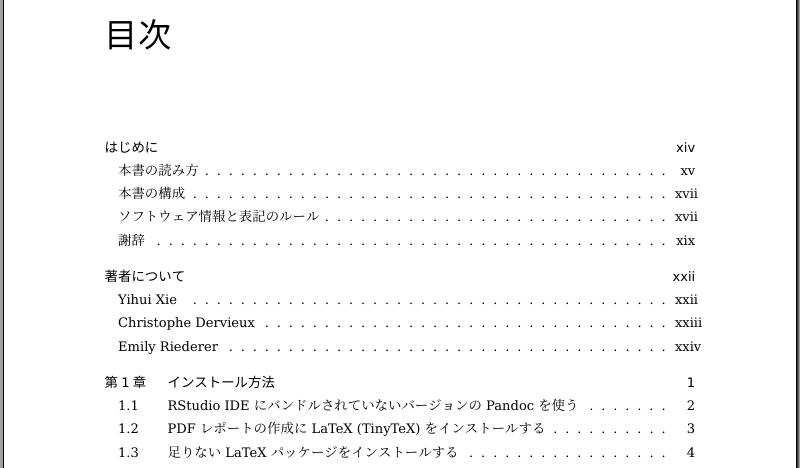
\includegraphics[width=1\linewidth,height=1\textheight,keepaspectratio]{JP/images/unnumbered-sections} 

}

\caption{付番された章とされていない章を示すための目次のスクリーンショット}\label{fig:unnumbered-sections}
\end{figure}

節番号は漸増します. もし付番されている節の後にされていない節が挿入し, その後にさらに付番された節が開始しているなら, 節番号はそこから増加を再開します.

\hypertarget{bibliography}{%
\section{参考文献と引用}\label{bibliography}}

参考文献の目録\index{bibliography}を出力文書に含める方法の概観として, \textcite{bookdown2016} の \href{https://bookdown.org/yihui/bookdown/citations.html}{Section 2.8} を見ることもできます. 基本的な使用法として, YAML\index{YAML!bibliography} メタデータの \texttt{bibliography} フィールドに文献目録ファイルを指定する必要があります. 例えば BibTeX データベースが \texttt{*.bib} という拡張子の付いたプレーンテキストとして与えられているなら, このようにします.

\begin{Shaded}
\begin{Highlighting}[]
\PreprocessorTok{{-}{-}{-}}
\FunctionTok{output}\KeywordTok{:}\AttributeTok{ html\_document}
\FunctionTok{bibliography}\KeywordTok{:}\AttributeTok{ references.bib  }
\PreprocessorTok{{-}{-}{-}}
\end{Highlighting}
\end{Shaded}

そしてこのファイルに文献アイテムがこのようなエントリで含まれています.

\begin{Shaded}
\begin{Highlighting}[]
\VariableTok{@Manual}\NormalTok{\{}\OtherTok{R}\NormalTok{{-}}\OtherTok{base}\NormalTok{,}
  \DataTypeTok{title}\NormalTok{ = \{R: A Language and Environment for Statistical}
\NormalTok{           Computing\},}
  \DataTypeTok{author}\NormalTok{ = \{\{R Core Team\}\},}
  \DataTypeTok{organization}\NormalTok{ = \{R Foundation for Statistical Computing\},}
  \DataTypeTok{address}\NormalTok{ = \{Vienna, Austria\},}
  \DataTypeTok{year}\NormalTok{ = \{2019\},}
  \DataTypeTok{url}\NormalTok{ = \{https://www.R{-}project.org\},}
\NormalTok{\}}
\end{Highlighting}
\end{Shaded}

文書内 \texttt{@key} という構文で文献アイテムを直接引用することができます. \texttt{key} の部分エントリの最初の行にある引用キーです. 上記の例なら \texttt{@R-base} です. 括弧で囲んで引用したいなら, \texttt{{[}@key{]}} を使います. 複数のエントリを同時に引用するなら, \texttt{{[}@key-1;\ @key-2;\ @key-3{]}} のようにセミコロンでキーを区切ります. 著者名を表示しないのなら, \texttt{{[}-@R-base{]}} のように \texttt{@} の前にマイナス記号を付けます.

\hypertarget{changing-citation-style}{%
\subsection{引用スタイルの変更}\label{changing-citation-style}}

デフォルトでは Pandoc は Chicago 式の著者名-出版年形式の引用\index{引用}スタイルと参考文献スタイルを使います. 他のスタイルを使うには, メタデータフィールド\index{YAML!csl}の \texttt{csl} で CSL (Citation Style Language) ファイルを指定します. 例えばこのように.

\begin{Shaded}
\begin{Highlighting}[]
\PreprocessorTok{{-}{-}{-}}
\FunctionTok{output}\KeywordTok{:}\AttributeTok{ html\_document}
\FunctionTok{bibliography}\KeywordTok{:}\AttributeTok{ references.bib}
\FunctionTok{csl}\KeywordTok{:}\AttributeTok{ biomed{-}central.csl}
\PreprocessorTok{{-}{-}{-}}
\end{Highlighting}
\end{Shaded}

必要としているフォーマットを見つけるには, \href{https://www.zotero.org/styles}{Zotero Style Repository,} を使うことをおすすめします. これは必要なスタイルの検索とダウンロードが簡単にできます.

CSL ファイルはカスタマイズされたフォーマット要件に合うようにを修正できます. 例えば ``et al.'' の前に表示する著者の人数を変更できます. これは \url{https://editor.citationstyles.org} で使用できるようなビジュアルエディタを使って簡単にできます.

\hypertarget{add-an-item-to-a-bibliography-without-using-it}{%
\subsection{引用していない文献を参考文献に追加する}\label{add-an-item-to-a-bibliography-without-using-it}}

デフォルトでは参考文献には文書で直接参照されたアイテムのみ表示されます. 本文中に実際に引用されていない文献を含めたい場合, \texttt{notice} というダミーのメタデータフィールド\index{YAML!nocite}を定義し, そこで引用します.

\begin{Shaded}
\begin{Highlighting}[]
\PreprocessorTok{{-}{-}{-}}
\FunctionTok{nocite}\KeywordTok{: }\CharTok{|}
\NormalTok{  @item1, @item2}
\PreprocessorTok{{-}{-}{-}}
\end{Highlighting}
\end{Shaded}

\hypertarget{add-all-items-to-the-bibliography}{%
\subsection{全てのアイテムを参考文献に掲載する}\label{add-all-items-to-the-bibliography}}

文献目録のすべてのアイテムを明示的に言及したくないが, 参考文献には掲載したいというなら, 以下のような構文が使えます.

\begin{Shaded}
\begin{Highlighting}[]
\PreprocessorTok{{-}{-}{-}}
\FunctionTok{nocite}\KeywordTok{:}\AttributeTok{ }\StringTok{\textquotesingle{}@*\textquotesingle{}}
\PreprocessorTok{{-}{-}{-}}
\end{Highlighting}
\end{Shaded}

これは全てのアイテムを参考文献として強制的に掲載させます.

\hypertarget{include-appendix-after-bibliography}{%
\subsection{参考文献の後に補遺を掲載する (*)}\label{include-appendix-after-bibliography}}

デフォルトでは参考文献は文書全体の最後に掲載されます. しかし参考文献一覧の後に追加のテキストを置きたいこともあるでしょう. 一番よくあるのは文書に補遺 (appendix) を含めたいときです. 以下に示すように, \texttt{\textless{}div\ id="refs"\textgreater{}\textless{}/div\textgreater{}} を使うことで参考文献一覧の位置を矯正できます.

\begin{Shaded}
\begin{Highlighting}[]
\FunctionTok{\# 参考文献}

\KeywordTok{\textless{}div}\OtherTok{ id=}\StringTok{"refs"}\KeywordTok{\textgreater{}\textless{}/div\textgreater{}}

\FunctionTok{\# 補遺}
\end{Highlighting}
\end{Shaded}

\texttt{\textless{}div\textgreater{}} は HTML タグですが, この方法は PDF など他の出力フォーマットでも機能します.

\textbf{bookdown} パッケージ \autocite{R-bookdown} を使うことで, 補遺の開始前に \href{https://bookdown.org/yihui/bookdown/markdown-extensions-by-bookdown.html\#special-headers}{special header} \texttt{\# (APPENDIX) Appendix \{-\}} の挿入が可能となり さらに改善できます. 例えば以下のように.

\begin{Shaded}
\begin{Highlighting}[]
\FunctionTok{\# 参考文献}

\KeywordTok{\textless{}div}\OtherTok{ id=}\StringTok{"refs"}\KeywordTok{\textgreater{}\textless{}/div\textgreater{}}

\FunctionTok{\# (APPENDIX) 補遺 \{{-}\} }

\FunctionTok{\# 追加情報}

\NormalTok{これは「補遺 A」になる.}

\FunctionTok{\# さらにもう1つ}

\NormalTok{これは「補遺 B」になる.}
\end{Highlighting}
\end{Shaded}

LaTeX/PDF および HTML フォーマットでは補遺の付番スタイルは自動的に変更されます (たいていは A, A.1, A.2, B, B.1, \ldots{} という形式です).

\hypertarget{write-bib}{%
\section{R パッケージの引用を生成する}\label{write-bib}}

R パッケージを引用するには, base R の \texttt{citation()}\index{utils!citation()} を使うことができます. BibTeX 用の引用エントリを生成したいなら, \texttt{citation()} の返り値を \texttt{toBibtex()}\index{utils!toBibtex()} を与えることができます. 例えばこうです.

\begin{Shaded}
\begin{Highlighting}[numbers=left,,]
\FunctionTok{toBibtex}\NormalTok{(}\FunctionTok{citation}\NormalTok{(}\StringTok{"xaringan"}\NormalTok{))}
\end{Highlighting}
\end{Shaded}

\begin{Shaded}
\begin{Highlighting}[]
\VariableTok{@Manual}\NormalTok{\{,}
  \DataTypeTok{title}\NormalTok{ = \{xaringan: Presentation Ninja\},}
  \DataTypeTok{author}\NormalTok{ = \{Yihui Xie\},}
  \DataTypeTok{year}\NormalTok{ = \{2020\},}
  \DataTypeTok{note}\NormalTok{ = \{R package version 0.19\},}
  \DataTypeTok{url}\NormalTok{ = \{https://CRAN.R{-}project.org/package=xaringan\},}
\NormalTok{\}}
\end{Highlighting}
\end{Shaded}

\texttt{toBibtex()} で生成されたエントリを使うには, 出力を \texttt{.bib} ファイルにコピーし, 引用キーを追加しなければなりません (例えば \texttt{@Manual\{,} の部分を \texttt{@Manual\{R-xaringan,} と書き換える). これは \texttt{knitr::write\_bib()}\index{knitr!write\_bib()} 関数によって自動化できます. この関数は引用エントリを生成し, 自動的にキーを加えてファイルに書き込みます. 例えばこのようにします.

\begin{Shaded}
\begin{Highlighting}[numbers=left,,]
\NormalTok{knitr}\SpecialCharTok{::}\FunctionTok{write\_bib}\NormalTok{(}\FunctionTok{c}\NormalTok{(}\FunctionTok{.packages}\NormalTok{(), }\StringTok{"bookdown"}\NormalTok{), }\StringTok{"packages.bib"}\NormalTok{)}
\end{Highlighting}
\end{Shaded}

第1引数はパッケージ名の文字列ベクトルで, 第2引数は \texttt{.bib} ファイルのパスであるべきです. 上記の例では, \texttt{.packages()} は現在の R セッションが読み込んでいる全てのパッケージ名を返します. これらのパッケージのいずれかが更新された (例えば著者, タイトル, 年, あるいはバージョンが変更された) とき, \texttt{write\_bib()} は自動的に \texttt{.bib} を更新できます.

引用エントリには2つのタイプが選択肢としてあります. 1つはパッケージの \texttt{DESCRIPTION} ファイルをもとに生成したもので, もう1つは, もしパッケージに \texttt{CITATION} ファイルが存在するなら, そこから生成したものです. 前者のタイプは引用キーが \texttt{R-(パッケージ名)} という形式になり (例えば \texttt{R-knitr}), 後者のタイプはパッケージ名と公開年を結合したものがキーとなります (例: \texttt{knitr2015}). もし複数のエントリが同一年にあるなら, 接尾文字が追加されます. 例えば \texttt{knitr2015a} と \texttt{knitr2015b} のように. 前者のタイプはしばしばパッケージ自体を引用 (つまり, ソフトウェアとして) するのに使われますが, 後者のタイプはしばしば論文や書籍のようなパッケージと関連のある出版物として扱われます.

\begin{Shaded}
\begin{Highlighting}[numbers=left,,]
\NormalTok{knitr}\SpecialCharTok{::}\FunctionTok{write\_bib}\NormalTok{(}\FunctionTok{c}\NormalTok{(}\StringTok{"knitr"}\NormalTok{, }\StringTok{"rmarkdown"}\NormalTok{), }\AttributeTok{width =} \DecValTok{60}\NormalTok{)}
\end{Highlighting}
\end{Shaded}

\begin{Shaded}
\begin{Highlighting}[]
\VariableTok{@Manual}\NormalTok{\{}\OtherTok{R}\NormalTok{{-}}\OtherTok{knitr}\NormalTok{,}
  \DataTypeTok{title}\NormalTok{ = \{knitr: A General{-}Purpose Package for Dynamic}
\NormalTok{    Report Generation in R\},}
  \DataTypeTok{author}\NormalTok{ = \{Yihui Xie\},}
  \DataTypeTok{year}\NormalTok{ = \{2021\},}
  \DataTypeTok{note}\NormalTok{ = \{R package version 1.31\},}
  \DataTypeTok{url}\NormalTok{ = \{https://yihui.org/knitr/\},}
\NormalTok{\}}

\VariableTok{@Manual}\NormalTok{\{}\OtherTok{R}\NormalTok{{-}}\OtherTok{rmarkdown}\NormalTok{,}
  \DataTypeTok{title}\NormalTok{ = \{rmarkdown: Dynamic Documents for R\},}
  \DataTypeTok{author}\NormalTok{ = \{JJ Allaire and Yihui Xie and Jonathan McPherson}
\NormalTok{    and Javier Luraschi and Kevin Ushey and Aron Atkins}
\NormalTok{    and Hadley Wickham and Joe Cheng and Winston Chang and}
\NormalTok{    Richard Iannone\},}
  \DataTypeTok{year}\NormalTok{ = \{2021\},}
  \DataTypeTok{note}\NormalTok{ = \{R package version 2.7\},}
  \DataTypeTok{url}\NormalTok{ = \{https://CRAN.R{-}project.org/package=rmarkdown\},}
\NormalTok{\}}

\VariableTok{@Book}\NormalTok{\{}\OtherTok{knitr2015}\NormalTok{,}
  \DataTypeTok{title}\NormalTok{ = \{Dynamic Documents with \{R\} and knitr\},}
  \DataTypeTok{author}\NormalTok{ = \{Yihui Xie\},}
  \DataTypeTok{publisher}\NormalTok{ = \{Chapman and Hall/CRC\},}
  \DataTypeTok{address}\NormalTok{ = \{Boca Raton, Florida\},}
  \DataTypeTok{year}\NormalTok{ = \{2015\},}
  \DataTypeTok{edition}\NormalTok{ = \{2nd\},}
  \DataTypeTok{note}\NormalTok{ = \{ISBN 978{-}1498716963\},}
  \DataTypeTok{url}\NormalTok{ = \{https://yihui.org/knitr/\},}
\NormalTok{\}}

\VariableTok{@InCollection}\NormalTok{\{}\OtherTok{knitr2014}\NormalTok{,}
  \DataTypeTok{booktitle}\NormalTok{ = \{Implementing Reproducible Computational}
\NormalTok{    Research\},}
  \DataTypeTok{editor}\NormalTok{ = \{Victoria Stodden and Friedrich Leisch and Roger}
\NormalTok{    D. Peng\},}
  \DataTypeTok{title}\NormalTok{ = \{knitr: A Comprehensive Tool for Reproducible}
\NormalTok{    Research in \{R\}\},}
  \DataTypeTok{author}\NormalTok{ = \{Yihui Xie\},}
  \DataTypeTok{publisher}\NormalTok{ = \{Chapman and Hall/CRC\},}
  \DataTypeTok{year}\NormalTok{ = \{2014\},}
  \DataTypeTok{note}\NormalTok{ = \{ISBN 978{-}1466561595\},}
  \DataTypeTok{url}\NormalTok{ = \{http://www.crcpress.com/product/isbn/}
\NormalTok{    9781466561595\},}
\NormalTok{\}}

\VariableTok{@Book}\NormalTok{\{}\OtherTok{rmarkdown2018}\NormalTok{,}
  \DataTypeTok{title}\NormalTok{ = \{R Markdown: The Definitive Guide\},}
  \DataTypeTok{author}\NormalTok{ = \{Yihui Xie and J.J. Allaire and Garrett}
\NormalTok{    Grolemund\},}
  \DataTypeTok{publisher}\NormalTok{ = \{Chapman and Hall/CRC\},}
  \DataTypeTok{address}\NormalTok{ = \{Boca Raton, Florida\},}
  \DataTypeTok{year}\NormalTok{ = \{2018\},}
  \DataTypeTok{note}\NormalTok{ = \{ISBN 9781138359338\},}
  \DataTypeTok{url}\NormalTok{ = \{https://bookdown.org/yihui/rmarkdown\},}
\NormalTok{\}}

\VariableTok{@Book}\NormalTok{\{}\OtherTok{rmarkdown2020}\NormalTok{,}
  \DataTypeTok{title}\NormalTok{ = \{R Markdown Cookbook\},}
  \DataTypeTok{author}\NormalTok{ = \{Yihui Xie and Christophe Dervieux and Emily}
\NormalTok{    Riederer\},}
  \DataTypeTok{publisher}\NormalTok{ = \{Chapman and Hall/CRC\},}
  \DataTypeTok{address}\NormalTok{ = \{Boca Raton, Florida\},}
  \DataTypeTok{year}\NormalTok{ = \{2020\},}
  \DataTypeTok{note}\NormalTok{ = \{ISBN 9780367563837\},}
  \DataTypeTok{url}\NormalTok{ = \{https://bookdown.org/yihui/rmarkdown{-}cookbook\},}
\NormalTok{\}}
\end{Highlighting}
\end{Shaded}

ファイルパスの引数がないと, \texttt{knitr::write\_bib()} は上記の例のように引用エントリをコンソールに出力します.

\texttt{write\_bib()} は既存の文献目録ファイルを上書きするように設計されていることに注意してください. 文献目録に手動で他のエントリを追加したい場合, 2つ目の \texttt{.bib} ファイルを作成して, この例のように \texttt{bibliography}\index{YAML!bibliography} フィールドで参照してください.

\begin{Shaded}
\begin{Highlighting}[]
\CommentTok{{-}{-}{-}}
\AnnotationTok{bibliography:}\CommentTok{ [packages.bib, references.bib]}
\CommentTok{{-}{-}{-}}

\InformationTok{\textasciigrave{}\textasciigrave{}\textasciigrave{}\{r, include=FALSE\}}
\InformationTok{knitr::write\_bib(file = \textquotesingle{}packages.bib\textquotesingle{})}
\InformationTok{\textasciigrave{}\textasciigrave{}\textasciigrave{}}
\end{Highlighting}
\end{Shaded}

上記の例では \texttt{packages.bib} が自動で生成されたもので, 手動で変更すべきではありません. それ以外の全ての引用エントリは \texttt{references.bib} に手動で書き込むことができます.

ここまでは R パッケージの引用を生成する方法を1つだけ紹介しています. それ以外のタイプの文献を動的に引用を生成するには, \textbf{knitcitations} パッケージ\index{R パッケージ!knitcitations} \autocite{R-knitcitations} を確認することもできます.

\hypertarget{cross-ref}{%
\section{文書内の相互参照}\label{cross-ref}}

相互参照\index{crossreference} はあなたの文書を通して読者を誘導するのに役に立つ方法であり, R Markdown ではこれを自動的に行なえます. これは \textbf{bookdown} 本の \href{https://bookdown.org/yihui/bookdown/components.html}{Chapter 2} で既に説明されていますが, 以下で簡潔な説明をします.

相互参照を使用するにあたって, 以下が必要になります.

\begin{itemize}
\item
  \textbf{bookdown 出力フォーマット}: 相互参照は基本となる \textbf{rmarkdown} パッケージでは直接提供されず, \textbf{bookdown} \autocite{R-bookdown} による拡張機能として提供されています. よって YAML の \texttt{output} フィールドで \textbf{bookdown} のフォーマット (例: \texttt{html\_document2}, \texttt{pdf\_document2}, \texttt{word\_document2} など) を使用しなければなりません.
\item
  \textbf{図 (または表) に対するキャプション}: キャプションのない図は単なる画像として直接埋め込まれるたあめ, 付番された図 (figure) にはなりません.
\item
  \textbf{ラベルの設定されたコードチャンク}:\index{code chunk!label} チャンクによって生成された図を参照するための識別子を提供してくれます.
\end{itemize}

これらの条件が合わさって初めて, テキスト内で \texttt{\textbackslash{}@ref(type:label)} という構文を使って相互参照を作成できます. \texttt{label} はチャンクラベルであり, \texttt{type} は参照するものの環境 (例:, \texttt{tab}, \texttt{fig}, \texttt{eqn}) です. 以下に例を示します.

\begin{Shaded}
\begin{Highlighting}[]
\CommentTok{{-}{-}{-}}
\AnnotationTok{title:}\CommentTok{ 図, 表, 数式を相互参照する}
\AnnotationTok{author:}\CommentTok{ bookdown による生成}
\AnnotationTok{output:}
\CommentTok{  bookdown::pdf\_document2:}
\CommentTok{    latex\_engine: lualatex}
\CommentTok{  bookdown::html\_document2: default}
\AnnotationTok{documentclass:}\CommentTok{ ltjsarticle}
\CommentTok{{-}{-}{-}}

\NormalTok{図 \textbackslash{}@ref(fig:cars{-}plot) を見よ.}

\InformationTok{\textasciigrave{}\textasciigrave{}\textasciigrave{}\{r cars{-}plot, fig.cap="自動車のデータ", echo=FALSE\}}
\InformationTok{par(mar = c(4, 4, .2, .1))}
\InformationTok{plot(cars)  \# a scatterplot}
\InformationTok{\textasciigrave{}\textasciigrave{}\textasciigrave{}}

\NormalTok{次に数式\textbackslash{}@ref(eq:mean) を見よ.}

\NormalTok{\textbackslash{}begin\{equation\}}
\NormalTok{\textbackslash{}bar\{X\} = \textbackslash{}frac\{\textbackslash{}sum\_\{i=1\}\^{}n X\_i\}\{n\} (}\SpecialCharTok{\textbackslash{}\#}\NormalTok{eq:mean)}
\NormalTok{\textbackslash{}end\{equation\}}

\NormalTok{さらに表 \textbackslash{}@ref(tab:mtcars) を見よ.}

\InformationTok{\textasciigrave{}\textasciigrave{}\textasciigrave{}\{r mtcars, echo=FALSE\}}
\InformationTok{knitr::kable(mtcars[1:5, 1:5], caption = "mtcars データ")}
\InformationTok{\textasciigrave{}\textasciigrave{}\textasciigrave{}}
\end{Highlighting}
\end{Shaded}

この文書の出力を図 \ref{fig:bookdown-ref} に示します.

\begin{figure}

{\centering 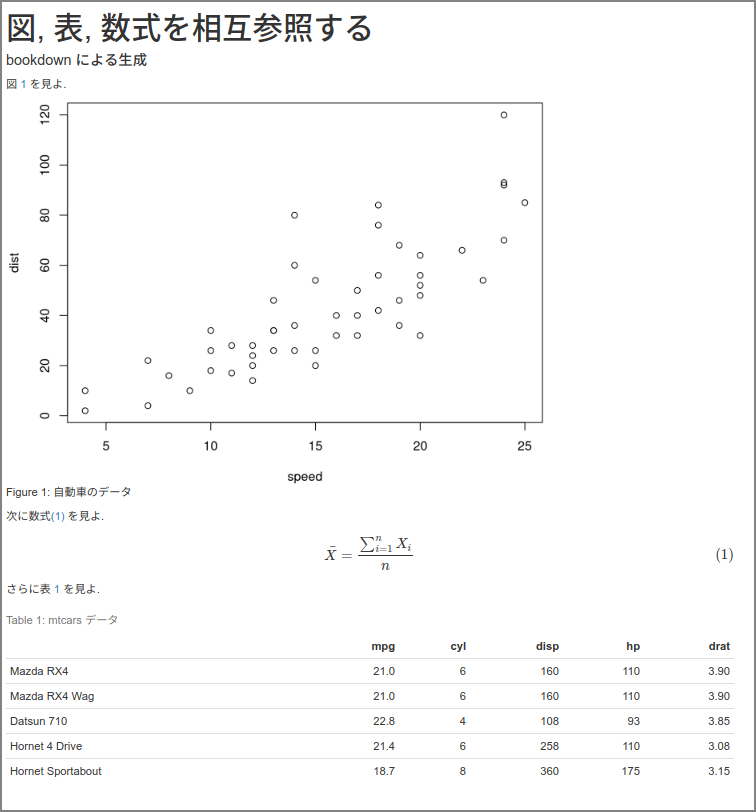
\includegraphics[width=1\linewidth,height=1\textheight,keepaspectratio]{JP/images/bookdown-ref} 

}

\caption{R Markdown 文書内の相互参照の例}\label{fig:bookdown-ref}
\end{figure}

数式, 定理, 節の見出しにも相互参照することができます. これらのタイプの参照は \textbf{bookdown} 本の 2.2, 2.6節でより説明されています.

\hypertarget{update-date}{%
\section{日付を自動的に更新する}\label{update-date}}

出力されたレポートに Rmd 文書がコンパイルされた日付を表示したいなら, YAML メタデータの \texttt{date} フィールド\index{YAML!date}にインライン R コードを追加し, 現在の日付を得るために \texttt{Sys.Date()} or \texttt{Sys.time()} 関数を使用できます.

\begin{Shaded}
\begin{Highlighting}[]
\FunctionTok{date}\KeywordTok{:}\AttributeTok{ }\StringTok{"\textasciigrave{}r Sys.Date()\textasciigrave{}"}
\end{Highlighting}
\end{Shaded}

もっと人間にとって読みやすい, 特定の日次フォーマットを指定したいかもしれません. 例えば以下のようにします.

\begin{Shaded}
\begin{Highlighting}[]
\FunctionTok{date}\KeywordTok{:}\AttributeTok{ }\StringTok{"\textasciigrave{}r format(Sys.time(), \textquotesingle{}\%x\textquotesingle{})\textasciigrave{}"}
\end{Highlighting}
\end{Shaded}

例えば 2021年3月21日 といったコードはあなたが文書を knit するごとに, 日付を動的に生成します. 日付のフォーマットをカスタマイズしたいならば, ご自分でフォーマット文字列を与えて変更できます. いくつか例をお見せしましょう.

\begin{itemize}
\tightlist
\item
  \texttt{\%Y \%B}: 2021 3月
\item
  \texttt{\%y/\%m/\%d}: 21/03/21
\item
  \texttt{\%b\%d (\%a)}: 3月21 (日)
\end{itemize}

表 \ref{tab:date-format} は POSIXct フォーマットの一覧です.

\begin{table}
\caption{\label{tab:date-format} Rにおける日付と時刻のフォーマット}\tabularnewline
\begin{tabular}{llll}
\toprule
コード & 意味 & コード & 意味\tabularnewline
\midrule

\%a & 曜日の略称 & \%A & 曜日の名称\tabularnewline
\%b & 月の略称 & \%B & 月の名称\tabularnewline
\%c & ロケール依存の時刻 & \%d & 数値表記の日\tabularnewline
\%H & 数値表記の時間 (24 時間) & \%I & 数値表記の時間 (12 時間)\tabularnewline
\%j & 1年の何日目か & \%m & 数値表記の月\tabularnewline
\%M & 数値表記の分 & \%p & ロケール依存の午前/午後\tabularnewline
\%S & 数値表記の秒 & \%U & 年の何週目か (日曜日始まり)\tabularnewline
\%w & 数値表記の曜日 (0=日曜日) & \%W & 年の何週目か (月曜日始まり)\tabularnewline
\%x & ロケール依存の日付 & \%X & ロケール依存の時刻\tabularnewline
\%y & 下2桁表記の年 & \%Y & 4桁表記の年\tabularnewline
\%z & GMT からのオフセット & \%Z & タイムゾーン (文字表記)\tabularnewline
\bottomrule
\end{tabular}
\end{table}

最後に, 説明的なテキストを日付に含めたいかもしれないときのことを書いておきます. このように Rコードの前に「最終コンパイル日」のような何らかの文を追加することができます.

\begin{Shaded}
\begin{Highlighting}[]
\FunctionTok{date}\KeywordTok{:}\AttributeTok{ }\StringTok{"最終コンパイル日 \textasciigrave{}r format(Sys.time(), \textquotesingle{}\%Y/\%m/\%d\textquotesingle{})\textasciigrave{}"}
\end{Highlighting}
\end{Shaded}

\hypertarget{multiple-authors}{%
\section{文書に複数の著者を表記する}\label{multiple-authors}}

R Markdown 文書のYAML フロントマターに複数の著者を加える方法は複数あります\index{YAML!author}. 単純に, 全員を同列に並べたい場合, 1つの文字列を与えることでできます. 例えばこのように.

\begin{Shaded}
\begin{Highlighting}[]
\PreprocessorTok{{-}{-}{-}}
\FunctionTok{title}\KeywordTok{:}\AttributeTok{ }\StringTok{"無題"}
\FunctionTok{author}\KeywordTok{:}\AttributeTok{ }\StringTok{"John Doe, Jane Doe"}
\PreprocessorTok{{-}{-}{-}}
\end{Highlighting}
\end{Shaded}

別の方法として, 各エントリごとに行を分けたいならば, YAML フィールドにエントリのリストを与えることができます. これは著者ごとにEメールアドレスや所属情報を加えたいときに役に立ちます. 例えばこのように.

\begin{Shaded}
\begin{Highlighting}[]
\PreprocessorTok{{-}{-}{-}}
\FunctionTok{author}\KeywordTok{:}
\AttributeTok{  }\KeywordTok{{-}}\AttributeTok{ John Doe, 組織1}
\AttributeTok{  }\KeywordTok{{-}}\AttributeTok{ Jane Doe, 組織2}
\PreprocessorTok{{-}{-}{-}}
\end{Highlighting}
\end{Shaded}

追加情報を文書の脚注として追記したい時, Markdown 構文の \texttt{\^{}{[}{]}} を利用できます. これは著者ごとに連絡先Eメールや住所といった多くの情報を含めたい場合により便利です. 厳密な動作は出力フォーマットに依存します.

\begin{Shaded}
\begin{Highlighting}[]
\PreprocessorTok{{-}{-}{-}}
\FunctionTok{author}\KeywordTok{:}
\AttributeTok{  }\KeywordTok{{-}}\AttributeTok{ John Doe\^{}[組織1, john@example.org]}
\AttributeTok{  }\KeywordTok{{-}}\AttributeTok{ Jane Doe\^{}[組織2, jane@example.org]}
\PreprocessorTok{{-}{-}{-}}
\end{Highlighting}
\end{Shaded}

特定の R Markdown テンプレートでは YAML に直接追加パラメータを指定することができます. 例えば \href{https://rstudio.github.io/distill/}{Distill} 出力フォーマットは \texttt{url}, \texttt{affiliation}, \texttt{affiliation\_url} を指定することが可能です. まずは \textbf{distill} パッケージ \autocite{R-distill}\index{R パッケージ!distill} をインストールします.

\begin{Shaded}
\begin{Highlighting}[numbers=left,,]
\FunctionTok{install.packages}\NormalTok{(}\StringTok{"distill"}\NormalTok{)}
\end{Highlighting}
\end{Shaded}

Distill フォーマットは詳細な著者情報を与えて使うことができます. 例えばこのように.

\begin{Shaded}
\begin{Highlighting}[]
\PreprocessorTok{{-}{-}{-}}
\FunctionTok{title}\KeywordTok{:}\AttributeTok{ }\StringTok{"R Markdown のための Distill"}
\FunctionTok{author}\KeywordTok{:}
\AttributeTok{  }\KeywordTok{{-}}\AttributeTok{ }\FunctionTok{name}\KeywordTok{:}\AttributeTok{ }\StringTok{"JJ Allaire"}
\AttributeTok{    }\FunctionTok{url}\KeywordTok{:}\AttributeTok{ https://github.com/jjallaire}
\AttributeTok{    }\FunctionTok{affiliation}\KeywordTok{:}\AttributeTok{ RStudio}
\AttributeTok{    }\FunctionTok{affiliation\_url}\KeywordTok{:}\AttributeTok{ https://www.rstudio.com}
\FunctionTok{output}\KeywordTok{:}\AttributeTok{ distill::distill\_article}
\PreprocessorTok{{-}{-}{-}}
\end{Highlighting}
\end{Shaded}

\hypertarget{figure-number}{%
\section{図のキャプションへの付番}\label{figure-number}}

\textbf{bookdown} \autocite{R-bookdown} 出力フォーマット\index{bookdown!html\_document2()} を, 図のキャプションに図番号を追加するのに使うことができます. 以下はその例です.

\begin{Shaded}
\begin{Highlighting}[]
\PreprocessorTok{{-}{-}{-}}
\FunctionTok{output}\KeywordTok{:}\AttributeTok{ bookdown::html\_document2}
\PreprocessorTok{{-}{-}{-}}
\end{Highlighting}
\end{Shaded}

\begin{Shaded}
\begin{Highlighting}[]
\InformationTok{\textasciigrave{}\textasciigrave{}\textasciigrave{}\{r cars, fig.cap = "すごいプロット"\}}
\InformationTok{plot(cars)}
\InformationTok{\textasciigrave{}\textasciigrave{}\textasciigrave{}}

\InformationTok{\textasciigrave{}\textasciigrave{}\textasciigrave{}\{r mtcars, fig.cap = "これもすごいプロット"\}}
\InformationTok{plot(mpg \textasciitilde{} hp, mtcars)}
\InformationTok{\textasciigrave{}\textasciigrave{}\textasciigrave{}}
\end{Highlighting}
\end{Shaded}

\ref{cross-ref} 節では表や数式といった他の要素でどのように動くか, そして付番された要素をテキスト内で相互参照する方法を実演しています. \texttt{html\_document2} いがいにも, \texttt{pdf\_document2}, \texttt{word\_document2} といった他の出力に対する同様のフォーマット関数もあります.

\textbf{bookdown} 以外の R Markdown 出力フォーマットにもこの機能を追加できます. 鍵はこれらが \textbf{bookdown} 出力フォーマットの「基本フォーマット」であることです. 例えば, \texttt{rticles::jss\_article} フォーマットで図に付番と相互参照をするために以下が使えます.

\begin{Shaded}
\begin{Highlighting}[]
\FunctionTok{output}\KeywordTok{:}
\AttributeTok{  bookdown::pdf\_book}\KeywordTok{:}\FunctionTok{}
\AttributeTok{    }\FunctionTok{base\_format}\KeywordTok{:}\AttributeTok{ rticles::jss\_article}
\end{Highlighting}
\end{Shaded}

\textbf{bookdown} 出力フォーマット関数のヘルプページを読んで, \texttt{base\_format} 引数\index{出力オプション!base\_format}があるかどうか確認してみてください (例: \texttt{?bookdown::html\_document2}).

\hypertarget{combine-words}{%
\section{単語をコンマ区切りで結合する}\label{combine-words}}

文字列ベクトルを人間の読みやすい形で出力したいとします. 例えば \texttt{x \textless{}-\ c("apple",\ "banana",\ "cherry")} について, きっとあなたは \texttt{{[}1{]}\ "apple"\ "banana"\ "cherry"} のような R が通常プリントする形式で出力をしてほしくないでしょう. あなたは代わりに ``\texttt{apple, banana, and cherry}'' という文字列がほしいのではないでしょうか. 文字列ベクトルを連結して1つにまとめる R 基本関数の \texttt{paste()} があります. 例えば \texttt{paste(x, collapse = \textquotesingle{},\ \textquotesingle{})} とすれば, 出力は \texttt{"apple, banana, cherry"} となるでしょう. この方法の問題は (1) 接続詞 ``and'' が欠けており, (2) ベクトルの要素が2つだけの場合はコンマを使うべきでない (\texttt{"apple, banana"} ではなく \texttt{"apple and banana"} という出力になるべき) ということです.

\texttt{knitr::combine\_words()}\index{knitr!combine\_words()} 関数は文字列ベクトルの長さにかかわらず, 要素を連結して文にできます. 基本的に, 単語1つに対してはそのまま同じものを返し, ``A and B'' という2つの単語に対しては \texttt{"A and B"} と返し, 3つ以上なら \texttt{"A, B, C, ..., Y, and Z"} というふうに返します. この関数はさらに出力をカスタマイズするいくつかの引数を持っています. 例えば出力される単語をバッククオートで囲みたいなら, \texttt{knitr::combine\_words(x, before = \textquotesingle{}\textasciigrave{}\textquotesingle{})} を使うこともできます. 以下に他の引数についてもさらなる例を示します. これらの出力例から引数の意味がよくわからないのであれば, ヘルプページ \texttt{?knitr::combine\_words} もご覧ください.

\begin{Shaded}
\begin{Highlighting}[numbers=left,,]
\NormalTok{v }\OtherTok{\textless{}{-}} \FunctionTok{c}\NormalTok{(}\StringTok{"apple"}\NormalTok{, }\StringTok{"banana"}\NormalTok{, }\StringTok{"cherry"}\NormalTok{)}
\NormalTok{knitr}\SpecialCharTok{::}\FunctionTok{combine\_words}\NormalTok{(v)}
\DocumentationTok{\#\# apple, banana, and cherry}
\NormalTok{knitr}\SpecialCharTok{::}\FunctionTok{combine\_words}\NormalTok{(v, }\AttributeTok{before =} \StringTok{"\textasciigrave{}"}\NormalTok{, }\AttributeTok{after =} \StringTok{"\textquotesingle{}"}\NormalTok{)}
\DocumentationTok{\#\# \textasciigrave{}apple\textquotesingle{}, \textasciigrave{}banana\textquotesingle{}, and \textasciigrave{}cherry\textquotesingle{}}
\NormalTok{knitr}\SpecialCharTok{::}\FunctionTok{combine\_words}\NormalTok{(v, }\AttributeTok{sep =} \StringTok{"、"}\NormalTok{, }\AttributeTok{and =} \StringTok{"そして"}\NormalTok{)}
\DocumentationTok{\#\# apple、banana、そしてcherry}
\NormalTok{knitr}\SpecialCharTok{::}\FunctionTok{combine\_words}\NormalTok{(v, }\AttributeTok{sep =} \StringTok{" / "}\NormalTok{, }\AttributeTok{and =} \StringTok{""}\NormalTok{)}
\DocumentationTok{\#\# apple / banana / cherry}
\NormalTok{knitr}\SpecialCharTok{::}\FunctionTok{combine\_words}\NormalTok{(v[}\DecValTok{1}\NormalTok{])  }\CommentTok{\# 単語1つ}
\DocumentationTok{\#\# apple}
\NormalTok{knitr}\SpecialCharTok{::}\FunctionTok{combine\_words}\NormalTok{(v[}\DecValTok{1}\SpecialCharTok{:}\DecValTok{2}\NormalTok{])  }\CommentTok{\# 単語2つ}
\DocumentationTok{\#\# apple and banana}
\NormalTok{knitr}\SpecialCharTok{::}\FunctionTok{combine\_words}\NormalTok{(LETTERS[}\DecValTok{1}\SpecialCharTok{:}\DecValTok{5}\NormalTok{])}
\DocumentationTok{\#\# A, B, C, D, and E}
\end{Highlighting}
\end{Shaded}

この関数はインライン R コードを使うときに特に使いやすいでしょう. 例えばこのように.

\begin{Shaded}
\begin{Highlighting}[]
\NormalTok{今朝は}\InformationTok{\textasciigrave{}r knitr::combine\_words(v, sep = \textquotesingle{}、\textquotesingle{}, and=\textquotesingle{}\textquotesingle{})\textasciigrave{}}\NormalTok{を食べた.}
\end{Highlighting}
\end{Shaded}

\hypertarget{linebreaks}{%
\section{複数の改行コードを維持する}\label{linebreaks}}

Markdown ユーザは, verbatim 環境 (コードブロック) 以外の場所では空白\index{改行} (改行コード含む) は大抵の場合意味を持たないことに気づき, 驚くでしょう. 2つ以上のスペースはスペース1つと同じであり, 改行1つはスペース1つと同じです. LaTeX や HTML を使ったことがあるなら, これらの言語と同じルールであるため驚くことはないかもしれません.

Markdown では, 空白行はしばしば段落などの要素の分離に使われます. 新しい段落に入らずに改行をするには, 末尾にスペース2つを追加しなければなりません. 特に詩や歌詞を引用したいときなど, 複数回改行したいときもあるかもしれません. 各行の末尾にスペース2つを手動で書き加えるのはうんざりする作業です. \texttt{blogdown:::quote\_poem()}\index{blogdown!quote\_poem()} はこの作業を自動でやってくれます. 例えばこのように.

\begin{Shaded}
\begin{Highlighting}[numbers=left,,]
\NormalTok{blogdown}\SpecialCharTok{:::}\FunctionTok{quote\_poem}\NormalTok{(}\FunctionTok{c}\NormalTok{(}\StringTok{"かたつむり"}\NormalTok{, }\StringTok{"そろそろ登れ"}\NormalTok{, }
  \StringTok{"富士の山"}\NormalTok{))}
\DocumentationTok{\#\# [1] "\textgreater{} かたつむり  \textbackslash{}nそろそろ登れ  \textbackslash{}n富士の山"}
\end{Highlighting}
\end{Shaded}

RStudio IDE と \textbf{blogdown} パッケージ \autocite{R-blogdown} をインストールして使っているなら, 改行を維持したいテキストを選択し, ツールバーの ``Addins'' から RStudio アドインの ``Quote Poem''\index{RStudio!Quote Poem アドイン} をクリックすることができます. 例えば以下のテキスト (fenced code block 記法内) は末尾にスペースが付いていません.

\begin{Shaded}
\begin{Highlighting}[]
\NormalTok{田子の浦ゆ}
\NormalTok{うち出でてみれば}
\NormalTok{真白にそ}
\NormalTok{富士の高嶺に}
\NormalTok{雪は降りける}

\NormalTok{{-}{-}{-} 山部赤人}
\end{Highlighting}
\end{Shaded}

上記の詩句を選択肢, RStudio アドインの ``Quote Poem'' をクリックすれば, こう出力されます.

\begin{quote}
田子の浦ゆ\\
うち出でてみれば\\
真白にそ\\
富士の高嶺に\\
雪は降りける

\begin{flushright}
--- 山部赤人

\end{flushright}
\end{quote}

TODO: quote poem だと flushrght が作られない?

時に「fenced code block は空白を維持するのに, 詩句をコードブロックに書くのはなぜですか」と質問があります. コードは詩的でありますが, 詩はコードではありません. 「コーディング」という行為にこだわりすぎないでください.

\hypertarget{equatiomatic}{%
\section{モデルを数式に変換する}\label{equatiomatic}}

Daniel Anderson らによって開発された \textbf{equatiomatic} パッケージ\index{R パッケージ!equatiomatic} \autocite{R-equatiomatic} (\url{https://github.com/datalorax/equatiomatic}) は R で当てはめたモデルに対応する数式を表示する, 便利な自動化の手段を提供します. 簡単な例を以下に示します.

\begin{Shaded}
\begin{Highlighting}[numbers=left,,]
\NormalTok{fit }\OtherTok{\textless{}{-}} \FunctionTok{lm}\NormalTok{(mpg }\SpecialCharTok{\textasciitilde{}}\NormalTok{ cyl }\SpecialCharTok{+}\NormalTok{ disp, mtcars)}
\CommentTok{\# 理論モデルを表示}
\NormalTok{equatiomatic}\SpecialCharTok{::}\FunctionTok{extract\_eq}\NormalTok{(fit)}
\end{Highlighting}
\end{Shaded}

\[
\operatorname{mpg} = \alpha + \beta_{1}(\operatorname{cyl}) + \beta_{2}(\operatorname{disp}) + \epsilon
\]

\begin{Shaded}
\begin{Highlighting}[numbers=left,,]
\CommentTok{\# 実際の係数を表示}
\NormalTok{equatiomatic}\SpecialCharTok{::}\FunctionTok{extract\_eq}\NormalTok{(fit, }\AttributeTok{use\_coefs =} \ConstantTok{TRUE}\NormalTok{)}
\end{Highlighting}
\end{Shaded}

\[
\operatorname{\widehat{mpg}} = 34.66 - 1.59(\operatorname{cyl}) - 0.02(\operatorname{disp})
\]

実際の数式を表示するには, チャンクオプション \texttt{results = "asis"}\index{チャンクオプション!results} (オプションの意味は\ref{results-asis}節参照) が必要です. そうしないと, テキスト出力がそのまま表示されてしまいます.

このパッケージについてより詳しく知りたいならば, ドキュメントを読み, Github 上での開発状況を追ってください.

\hypertarget{animation}{%
\section{複数の R プロットからアニメーションを作成する}\label{animation}}

1つのコードチャンクで一連のプロットを生成したとき, これらを結合し1つのアニメーション\index{アニメーション}を生成できます. 出力フォーマットが HTML なら, これは簡単です. \textbf{gifski} パッケージ\index{R パッケージ!gifski} \autocite{R-gifski} をインストールし, チャンクオプション \texttt{animation.hook = "gifski"}\index{チャンクオプション!animation.hook} 設定するだけです. 図\ref{fig:pacman} はシンプルな「パックマン」のアニメーションで, これは以下のコードで作成しました.

\begin{Shaded}
\begin{Highlighting}[]
\InformationTok{\textasciigrave{}\textasciigrave{}\textasciigrave{}\{r, animation.hook="gifski"\}}
\InformationTok{for (i in 1:2) \{}
\InformationTok{  pie(c(i \%\% 2, 6), col = c(\textquotesingle{}red\textquotesingle{}, \textquotesingle{}yellow\textquotesingle{}), labels = NA)}
\InformationTok{\}}
\InformationTok{\textasciigrave{}\textasciigrave{}\textasciigrave{}}
\end{Highlighting}
\end{Shaded}

\begin{figure}

{\centering \includegraphics[width=0.5\linewidth,height=1\textheight,keepaspectratio]{rmarkdown-cookbook_files/figure-latex/pacman-1} \includegraphics[width=0.5\linewidth,height=1\textheight,keepaspectratio]{rmarkdown-cookbook_files/figure-latex/pacman-2} 

}

\caption{パックマンのアニメーション}\label{fig:pacman}
\end{figure}

アニメーションのフォーマットは GIF で, HTML 出力ではうまく動作しますが, LaTeX は GIF を直接サポートしていません. あなたが本書の PDF または印刷版を読んでいるなら, 図\ref{fig:pacman} が2つの動かない画像になっているのはこれが理由です. 本書のオンライン版を読めば, 実際のアニメーションが見られるでしょう.

PDF でもアニメーションを動作させることはできますが, 事前準備が2つ必要です. 第1に, LaTeX パッケージの \href{https://ctan.org/pkg/animate}{\textbf{animate}} を読み込む必要があります (方法は\ref{latex-extra}節参照). 第2に, Acrobat Reader でのみアニメーションを見ることができます. 第2位に, Acrobat Reader でのみアニメーションの動作を見ることができます. それからチャンクオプション \texttt{fig.show = "animate"}\index{チャンクオプション!fig.show} で \textbf{animate} パッケージ\index{R パッケージ!animate} を使いアニメーションを作成できるようにします. 以下はその例です.

\begin{Shaded}
\begin{Highlighting}[]
\CommentTok{{-}{-}{-}}
\AnnotationTok{title:}\CommentTok{ PDF でのアニメーション}
\AnnotationTok{output:}
\CommentTok{  pdf\_document:}
\CommentTok{    extra\_dependencies: animate}
\CommentTok{{-}{-}{-}}

\NormalTok{以下のアニメーションは Acrobat Reader でのみ見ることができます.}

\InformationTok{\textasciigrave{}\textasciigrave{}\textasciigrave{}\{r, fig.show=\textquotesingle{}animate\textquotesingle{}\}}
\InformationTok{for (i in 1:2) \{}
\InformationTok{  pie(c(i \%\% 2, 6), col = c(\textquotesingle{}red\textquotesingle{}, \textquotesingle{}yellow\textquotesingle{}), labels = NA)}
\InformationTok{\}}
\InformationTok{\textasciigrave{}\textasciigrave{}\textasciigrave{}}
\end{Highlighting}
\end{Shaded}

アニメーションのイメージフレーム間の表示間隔はチャンクオプション \texttt{interval}\index{チャンクオプション!interval} で設定できます. デフォルトでは \texttt{interval = 1} (つまり1秒) です.

R パッケージ \textbf{animation}\index{R パッケージ!animation} \autocite{R-animation} には, 統計的計算の方法やアイディアを表現するアニメーションの例がいくつか入っています. \textbf{gganimate} パッケージ\index{R パッケージ!gganimate} \autocite{R-gganimate} は \textbf{ggplot2}\index{R パッケージ!gglot2} \autocite{R-ggplot2} に基づいた滑らかなアニメーションの作成を可能にします. どちらも R Markdown で動作します.

\hypertarget{diagrams}{%
\section{ダイアグラムを作成する}\label{diagrams}}

ダイアグラム\index{図!ダイアグラムの作成}やフローチャートを生成する, R とは独立したプログラム (例: Graphviz) は多くありますが, これらは Rmd 文書内のコードチャンク内で直接管理することができます.

R ではいくつかのパッケージが使用可能ですが, その中で \textbf{DiagrammeR}\index{R パッケージ!DiagrammeR} \autocite{R-DiagrammeR} とその他いくつかを最後に簡単に解説します. 完全なデモは \url{https://rich-iannone.github.io/DiagrammeR/} で見ることができます. この節では基本的な使用法とダイアグラム内で R コードを使う方法を紹介します.

\hypertarget{basic-diagrams}{%
\subsection{基本的なダイアグラム}\label{basic-diagrams}}

\textbf{DiagrammeR} はいくつかの異なるグラフ言語を使ってグラフを作成する方法を提供します. この節では Graphviz の例を提示しますが,\footnote{あなたのバックグラウンド次第では, この節は \textbf{DiagrammeR} に対する偏った解説になるかもしれません. このパッケージに興味があるなら, パッケージの公式ドキュメントをご覧ください.} \textbf{DiagrammeR} は純粋に R コードだけでグラフを作ることもできます.

RStudio IDE は Graphviz (\texttt{.gv}) および mermaid (\texttt{.mmd}) ファイルをネイティブにサポートしています. これらのタイプのファイルを RStudio で編集すると, シンタックスハイライトされるという利点があります. RStudio のツールバーの ``Preview'' ボタンをクリックすると, ダイアグラムをプレビューすることができます. 図\ref{fig:diagram-profit} は, 4つのステップを表す矩形で構成された, フローチャートの単純な例です. これは以下のコードで生成されています.

\begin{Shaded}
\begin{Highlighting}[numbers=left,,]
\NormalTok{DiagrammeR}\SpecialCharTok{::}\FunctionTok{grViz}\NormalTok{(}\StringTok{"digraph \{}
\StringTok{  graph [layout = dot, rankdir = TB]}
\StringTok{  }
\StringTok{  node [shape = rectangle]        }
\StringTok{  rec1 [label = \textquotesingle{}ステップ 1. 起床する\textquotesingle{}]}
\StringTok{  rec2 [label = \textquotesingle{}ステップ 2. コードを書く\textquotesingle{}]}
\StringTok{  rec3 [label =  \textquotesingle{}ステップ 3. ???\textquotesingle{}]}
\StringTok{  rec4 [label = \textquotesingle{}ステップ 4. 収入を得る\textquotesingle{}]}
\StringTok{  }
\StringTok{  \# ノードIDでエッジを定義}
\StringTok{  rec1 {-}\textgreater{} rec2 {-}\textgreater{} rec3 {-}\textgreater{} rec4}
\StringTok{  \}"}\NormalTok{, }
  \AttributeTok{height =} \DecValTok{500}\NormalTok{)}
\end{Highlighting}
\end{Shaded}

\begin{figure}

{\centering \includegraphics[width=1\linewidth,height=1\textheight,keepaspectratio]{rmarkdown-cookbook_files/figure-latex/diagram-profit-1} 

}

\caption{プログラマの絵空事を表したダイアグラム}\label{fig:diagram-profit}
\end{figure}

ノードの形状, 色, 線のタイプを定義したり, パラメータを追加したりといったことができる拡張的な操作も用意されています.

\hypertarget{adding-parameters-to-plots}{%
\subsection{図にパラメータを追加する}\label{adding-parameters-to-plots}}

Graphviz の置換機能は可読性を損なうことなく, R 評価式を Graphviz のグラフ設定に混ぜ込むことができます. \texttt{@@} を伴う置換を指定すれば, そこに置換される有効な R 評価式が確実にあるようにせねばなりません. 評価式は脚注として置かれ, そして R ベクトルオブジェクトを返すものでなくてはなりません. \texttt{@@} という記法のすぐ後には数字が続き, これは R 評価式の脚注番号に対応します. 図\ref{fig:diagram-params}はダイアグラムへの R コードの埋め込みと評価の例です.

\begin{Shaded}
\begin{Highlighting}[numbers=left,,]
\NormalTok{DiagrammeR}\SpecialCharTok{::}\FunctionTok{grViz}\NormalTok{(}\StringTok{"}
\StringTok{  digraph graph2 \{}
\StringTok{  }
\StringTok{  graph [layout = dot, rankdir = LR]}
\StringTok{  }
\StringTok{  \# node definitions with substituted label text}
\StringTok{  node [shape = oval]}
\StringTok{  a [label = \textquotesingle{}@@1\textquotesingle{}]}
\StringTok{  b [label = \textquotesingle{}@@2\textquotesingle{}]}
\StringTok{  c [label = \textquotesingle{}@@3\textquotesingle{}]}
\StringTok{  d [label = \textquotesingle{}@@4\textquotesingle{}]}
\StringTok{  }
\StringTok{  a {-}\textgreater{} b {-}\textgreater{} c {-}\textgreater{} d}
\StringTok{  \}}
\StringTok{  }
\StringTok{  [1]: names(iris)[1]}
\StringTok{  [2]: names(iris)[2]}
\StringTok{  [3]: names(iris)[3]}
\StringTok{  [4]: names(iris)[4]}
\StringTok{  "}\NormalTok{, }
  \AttributeTok{height =} \DecValTok{100}\NormalTok{)}
\end{Highlighting}
\end{Shaded}

\begin{figure}

{\centering \includegraphics[width=1\linewidth,height=1\textheight,keepaspectratio]{rmarkdown-cookbook_files/figure-latex/diagram-params-1} 

}

\caption{R から入力されたパラメータを使用したダイアグラム}\label{fig:diagram-params}
\end{figure}

\hypertarget{other-packages-for-making-diagrams}{%
\subsection{その他のダイアグラム作成パッケージ}\label{other-packages-for-making-diagrams}}

ダイアグラム作成に使えるパッケージとして, \textbf{nomnoml} \autocite{R-nomnoml}, \textbf{diagram} \autocite{R-diagram}, \textbf{dagitty} \autocite{R-dagitty}, \textbf{ggdag} \autocite{R-ggdag}, \textbf{plantuml} (\url{https://github.com/rkrug/plantuml}) といったものを確かめることになるかもしません.

\hypertarget{special-chars}{%
\section{特殊文字をエスケープする}\label{special-chars}}

Markdown 構文で特殊な意味を持つ文字がいくつかあります. これらの文字を直接使いたい場合, エスケープしなければなりません. 例えばテキストを囲むアンダースコアの組はたいていの場合テキストをイタリック体にします. イタリック体ではなく, アンダースコアをそのまま表示させたいなら, アンダースコアをエスケープする必要があります. 特殊な文字をエスケープする方法は, その直前にバックスラッシュを付けることです. 例えば「\texttt{ここは\textbackslash{}\_イタリックに\textbackslash{}\_したくない.}」というふうに. 同様に, \texttt{\#} をセクションヘッダを表してほしくないなら, \texttt{\textbackslash{}\#\ これは見出しではない} などと書くこともできます.

\ref{linebreaks} 節で言及したように, 連続した空白文字は1つの正規スペースとして表示されます. 書いたとおりに連続した空白文字を表示させたいならば, 1つ1つにエスケープが必要です. 例えば \texttt{ソーシャル \textbackslash{}\ \textbackslash{}\ \textbackslash{}\ ディスタンス維持} というふうに. 空白がエスケープされた時, 空白は「改行しない空白」に変換されます. これは, そのスペースの位置では行が折り返されないということです. 例えば \texttt{Mr.\textbackslash{}\ Dervieux} と言うふうに. TODO: ここもしかして折返しが発生するように調整されてる?

\hypertarget{comments}{%
\section{テキストのコメントアウト}\label{comments}}

ソース文書内のテキストを最終的な出力文書に表示させないようコメントアウト\index{コメント}するのはとても便利です. この用途のため, HTML の構文である \texttt{\textless{}!-\/-\ ここにコメント\ -\/-\textgreater{}} を使えます. コメントはどの出力形式にも表示されません.

コメントは1行でも, 複数行にも広げられます. これは草稿を書くのに便利でしょう.

RStudio を使うなら, 1行丸ごとコメントアウトするのにキーボードショートカット\index{RStudio!コメントのショートカット} \texttt{Ctrl + Shift + C} (MacOS なら\texttt{Command + Shift + C}) を使えます.

\hypertarget{toc-unlisted}{%
\section{目次から見出しを省略する}\label{toc-unlisted}}

目次に特定のセクションの見出しを表示させたくないなら, 見出しに2つのクラスを追加できます. \texttt{unlisted}\index{クラス!unlisted} と \texttt{unnumbered}\index{クラス!unnumbered} です. 例えばこのように

\begin{Shaded}
\begin{Highlighting}[]
\FunctionTok{\# 見出し \{.unlisted .unnumbered\}}
\end{Highlighting}
\end{Shaded}

この機能は Pandoc 2.10 以降のバージョンが必要です. \texttt{rmarkdown::pandoc\_version()} で Pandoc のバージョンを確認しましょう. バージョンが 2.10 より古いなら, 新しいバージョンをインストールすることになるでしょう (\ref{install-pandoc}節参照).

\hypertarget{code-appendix}{%
\section{全てのコードを補遺に置く (*)}\label{code-appendix}}

対象読者がレポートを読む時, 計算の詳細に強く関心があるのでない限り, あなたはレポートにソースコードブロックを表示させたくないかもしれません. この用途で, チャンクオプション \texttt{echo = FALSE}\index{チャンクオプション!echo} を設定してソースコードを隠し, 読者がプログラムコードで気が散らないようにすることができます. しかしそれでも, ソースコードは再現可能性のある研究のために重要です. 読者はレポートを読み終わった後に計算の正しさを検証したいと思うかも知れません. この場合, 本文中の全てのコードブロックをまとめ, 文書の末尾 (例えば補遺として) に表示するというのは良い考えでしょう.

チャンクオプションの \texttt{ref.label}\index{チャンクオプション!ref.label} と \texttt{knitr::all\_labels()}\index{knitr!all\_labels()} 関数を使い, 文書内の全てのコードチャンクを取り出して1つのコードチャンクにまとめる簡単な方法があります. 例えばこのように.

\begin{Shaded}
\begin{Highlighting}[]
\FunctionTok{\# 補遺: 本稿で使ったコード全文}

\InformationTok{\textasciigrave{}\textasciigrave{}\textasciigrave{}\{r ref.label=knitr::all\_labels(), echo=TRUE, eval=FALSE\}}
\InformationTok{\textasciigrave{}\textasciigrave{}\textasciigrave{}}
\end{Highlighting}
\end{Shaded}

チャンクオプション \texttt{ref.label} について詳しく知らないならば, \ref{ref-label}節を読んでください.

\texttt{knitr::all\_labels()} 関数は文書内の全てのチャンクラベルを返すため, \texttt{ref.label = knitr::all\_labels()} は全てのソースコードチャンクを回収しこのチャンクに持ってくることを意味します. チャンクオプション \texttt{echo = TRUE} (コードを表示させる) と \texttt{eval = FALSE}\index{チャンクオプション!eval} (全てのコードはすでに実行されているため, このコードチャンクは実行してはいけません) を付与すれば, 1つのコードチャンクに全てのソースコードのコピーを表示させられます.

\texttt{ref.label} は任意のチャンクラベルの文字列ベクトルであるため, 補遺に表示するコードチャンクを一部だけにするようにラベルをフィルタリングできます. 以下はその例 (\href{https://yihui.org/en/2018/09/code-appendix/}{Ariel Muldoon} によるものです) として \texttt{setup} と \texttt{get-labels} というラベルを排除しています.

\begin{Shaded}
\begin{Highlighting}[]
\InformationTok{\textasciigrave{}\textasciigrave{}\textasciigrave{}\{r get{-}labels, echo = FALSE\}}
\InformationTok{labs = knitr::all\_labels()}
\InformationTok{labs = setdiff(labs, c("setup", "get{-}labels"))}
\InformationTok{\textasciigrave{}\textasciigrave{}\textasciigrave{}}

\InformationTok{\textasciigrave{}\textasciigrave{}\textasciigrave{}\{r all{-}code, ref.label=labs, eval=FALSE\}}
\InformationTok{\textasciigrave{}\textasciigrave{}\textasciigrave{}}
\end{Highlighting}
\end{Shaded}

\texttt{knitr::all\_labels()} の引数を使ってコードチャンクをフィルタリングすることもできます. 例えば \texttt{Rcpp} エンジン (\texttt{engine == "Rcpp"}) を使用した全てのコードチャンクを得て, かつ文書に表示しない (\texttt{echo = FALSE}) ようにするには \texttt{knitr::all\_labels(engine == "Rcpp", echo == FALSE)} を使うこともできます. どのコードチャンクを補遺に表示したいのか, 正確にコントロールしたいならば, 指定したいコードチャンクに特殊なチャンクオプション \texttt{appendix = TRUE} を使い, それらのチャンクのラベルを得るのに \texttt{ref.label = knitr::all\_labels(appendix == TRUE)} を使うこともできます.

\hypertarget{lua-filters}{%
\section{Pandoc の Lua フィルタから操作する (*)}\label{lua-filters}}

\index{Pandoc!Lua フィルタ|see  {Lua フィルタ}}

技術的にはこの節は少し発展的ですが, Markdown の内容が Pandoc 抽象構文木 (AST) にどのように翻訳されるかを一度学べば, Lua というプログラミング言語を使ってどのような Markdown の要素も操作する力を得ることになります.

基本として, Pandoc は Markdown ファイルを読み取り, その内容が AST にパースされます. Pandoc はこの AST をLua スクリプト\index{Lua フィルタ}を使って修正することを可能にします. AST の意味するものを示すため, 以下のような簡単な Markdown ファイル (\texttt{ast.md}) を使います.

\begin{Shaded}
\begin{Highlighting}[numbers=left,,]
\FunctionTok{\#\# 第1節}

\NormalTok{Hello world!}
\end{Highlighting}
\end{Shaded}

このファイルは見出し1つとパラグラフ1つを持っています. Pandoc がこの内容をパースした後ファイルを JSON 形式に変換すれば, R ユーザーにとっては 結果として現れる AST を理解するよりも簡単でしょう.

\begin{Shaded}
\begin{Highlighting}[numbers=left,,]
\ExtensionTok{pandoc}\NormalTok{ {-}f markdown {-}t json {-}o ast.json ast.md}
\end{Highlighting}
\end{Shaded}

そして JSON ファイルを R に読み込み, データ構造を書き出します.

この操作をしたら, Markdown の内容は再帰的なリストで表現されていることが分かるでしょう. その構造を以下に表します. ラベル \texttt{t} は ``type'', \texttt{c} は ``content'' を表します. 例として見出しを取り上げてみましょう. タイプは ``Header'' で, その中身は3つの要素が含まれています. 見出しのレベル (\texttt{2}), 属性 (例えば ID が \texttt{section-one} であること), そしてテキストの内容です.

\begin{Shaded}
\begin{Highlighting}[numbers=left,,]
\NormalTok{xfun}\SpecialCharTok{:::}\FunctionTok{tree}\NormalTok{(}
\NormalTok{  jsonlite}\SpecialCharTok{::}\FunctionTok{fromJSON}\NormalTok{(}\StringTok{\textquotesingle{}ast.json\textquotesingle{}}\NormalTok{, }\AttributeTok{simplifyVector =} \ConstantTok{FALSE}\NormalTok{)}
\NormalTok{)}
\end{Highlighting}
\end{Shaded}

\begin{verbatim}
List of 3
 |-blocks            :List of 2
 |  |-:List of 2
 |  |  |-t: chr "Header"
 |  |  |-c:List of 3
 |  |     |-: int 2
 |  |     |-:List of 3
 |  |     |  |-: chr "第1節"
 |  |     |  |-: list()
 |  |     |  |-: list()
 |  |     |-:List of 1
 |  |        |-:List of 2
 |  |           |-t: chr "Str"
 |  |           |-c: chr "第1節"
 |  |-:List of 2
 |     |-t: chr "Para"
 |     |-c:List of 3
 |        |-:List of 2
 |        |  |-t: chr "Str"
 |        |  |-c: chr "Hello"
 |        |-:List of 1
 |        |  |-t: chr "Space"
 |        |-:List of 2
 |           |-t: chr "Str"
 |           |-c: chr "world!"
 |-pandoc-api-version:List of 2
 |  |-: int 1
 |  |-: int 20
 |-meta              : Named list()
\end{verbatim}

あなたが AST に気づけば, Lua によって修正することができます. Pandoc は組み込みの Lua インタプリタを持っているので, 追加でツールをインストールする必要はありません. Lua スクリプトは Pandoc では「Lua フィルタ」と呼ばれます. 次に見出しのレベルを1増やす, 例えばレベル3の見出しを2に変換する簡単な例を見せます. これは文書のトップレベルの見出しがレベル2で, 代わりにレベル1から始めたい場合に便利です.

最初に \texttt{raise-header.lua} という名前の Lua スクリプトファイルを作ります. これには \texttt{Header} という名前の関数が含まれており, ``Header'' タイプの要素を修正したいということを意味しています (一般に, あるタイプの要素を処理するためにタイプ名を関数名として使うことができます).

\begin{Shaded}
\begin{Highlighting}[numbers=left,,]
\KeywordTok{function}\NormalTok{ Header}\OperatorTok{(}\NormalTok{el}\OperatorTok{)}
  \CommentTok{{-}{-} 見出しのレベルは要素の持つ \textquotesingle{}level\textquotesingle{} 属性でアクセスできます.}
  \CommentTok{{-}{-} 後述の Pandoc ドキュメントを見てください.}
  \ControlFlowTok{if} \OperatorTok{(}\NormalTok{el}\OperatorTok{.}\NormalTok{level }\OperatorTok{\textless{}=} \DecValTok{1}\OperatorTok{)} \ControlFlowTok{then}
    \FunctionTok{error}\OperatorTok{(}\StringTok{"h1 のレベルを上げる方法がわかりません"}\OperatorTok{)}
  \ControlFlowTok{end}
\NormalTok{  el}\OperatorTok{.}\NormalTok{level }\OperatorTok{=}\NormalTok{ el}\OperatorTok{.}\NormalTok{level }\OperatorTok{{-}} \DecValTok{1}
  \ControlFlowTok{return}\NormalTok{ el}
\KeywordTok{end}
\end{Highlighting}
\end{Shaded}

そしてこのスクリプト Pandoc の \texttt{-\/-lua-filter} 引数に与えることができます. 例えばこうです.

\begin{Shaded}
\begin{Highlighting}[numbers=left,,]
\ExtensionTok{pandoc}\NormalTok{ {-}t markdown {-}{-}atx{-}headers }\KeywordTok{\textbackslash{}}
  \ExtensionTok{{-}{-}lua{-}filter}\NormalTok{=raise{-}header.lua ast.md}
\end{Highlighting}
\end{Shaded}

\begin{verbatim}
# 第1節

Hello world!
\end{verbatim}

\texttt{\#\# Section One} を \texttt{\# Section One} へ変換することに成功したのがお分かりかと思います. この例は些細なものだと思うかも知れませんし, なんでこんなふうに単に正規表現を使って \texttt{\#\#} を \texttt{\#} に置き換えないのかと思うかも知れません.

\begin{Shaded}
\begin{Highlighting}[numbers=left,,]
\FunctionTok{gsub}\NormalTok{(}\StringTok{"\^{}\#\#"}\NormalTok{, }\StringTok{"\#"}\NormalTok{, }\FunctionTok{readLines}\NormalTok{(}\StringTok{"ast.md"}\NormalTok{))}
\end{Highlighting}
\end{Shaded}

例えば \texttt{\#\#} が R コード内でコメントに使われていたら, と言うふうに, 正規表現はほとんど常に例外があるため, たいていの場合で, 構造化された文書を操作するのにロバストな手段ではありません. AST は構造化されたデータを与えてくれるので, 確実に意図した要素を修正していることが分かります.

Pandoc の Lua フィルタに関する追加ドキュメントが \url{https://pandoc.org/lua-filters.html} にあり, ここで多くの例を見つけることができます. GitHub リポジトリ \url{https://github.com/pandoc/lua-filters} のコミュニティで書かれたフィルタを見つけることもできます.

R Markdown の世界では Lua フィルタを活用しているパッケージの例の一部が以下になります (たいていは \texttt{inst/} ディレクトリにあります)

\begin{itemize}
\item
  \textbf{rmarkdown} パッケージ (\url{https://github.com/rstudio/rmarkdown}) は改行 (\ref{pagebreaks}節参照) を挿入するフィルタとカスタムブロック (\ref{custom-blocks}節参照)を生成するフィルタを含んでいます.
\item
  \textbf{pagedown} パッケージ \autocite{R-pagedown} には脚注を実装するのを助けるフィルタと HTML ページに図のリストを表示するフィルタがあります.
\item
  \textbf{govdown} パッケージ \autocite{R-govdown} には Pandoc の \texttt{Div} による囲みを適切な HTML タグに変換するフィルタがあります.
\end{itemize}

本書の\ref{lua-color}節でも Lua フィルタでテキストの色を変更する方法を紹介する例を見ることができます.

Lua フィルタを (上記のパッケージのように) 導入するために R パッケージ を作りたくない R Markdown ユーザーは, これらの Lua スクリプトをコンピュータのどこかに保存し, R Markdown 出力フォーマットの \texttt{pandoc\_args}\index{出力オプション!pandoc\_args} オプションで適用することもできます. 例えばこのように.

\begin{Shaded}
\begin{Highlighting}[]
\PreprocessorTok{{-}{-}{-}}
\FunctionTok{output}\KeywordTok{:}
\AttributeTok{  }\FunctionTok{html\_document}\KeywordTok{:}
\AttributeTok{    }\FunctionTok{pandoc\_args}\KeywordTok{:}
\AttributeTok{      }\KeywordTok{{-}}\AttributeTok{ {-}{-}lua{-}filter=raise{-}header.lua}
\PreprocessorTok{{-}{-}{-}}
\end{Highlighting}
\end{Shaded}

\hypertarget{formatting}{%
\chapter{書式}\label{formatting}}

Markdown 言語の最大の強みは, その簡潔さが初心者にとっても読み書きを非常に簡単にさせていることです. これはオリジナルの Markdown 言語の考案者も次のようにまとめている設計原理の鍵です.

\begin{quote}
Markdown 形式の文書は見たままに, タグや整形の指示文でマークアップされず, プレーンテキストとして出力されるべきである.

\begin{flushright}
--- \href{http://daringfireball.net/projects/markdown/syntax\#philosophy}{John Gruber}

\end{flushright}
\end{quote}

しかし, これはカスタマイズのコストがかかります. 典型的なワードプロセッサの多くの機能は Markdown で直接使うことができません. 例えば以下のような機能です.

\begin{itemize}
\item
  テキストの一部のフォントサイズを変更する
\item
  ある単語のフォント色を変更する
\item
  テキストアラインメントを指定する
\end{itemize}

こういった機能があなたの努力に見合うかどうかはあなたの判断に委ねます. Markdown は,「自然界」はプレーンテキストからなり, (見た目上の) 面白さを欲求して\textbf{作為}すべきではない, というストア派哲学をいくらか反映しています. いずれにせよ, この章では R Markdown 文書の見た目や要素のスタイルをカスタマイズをどうやればできるかの豆知識をいくつか提示します.

Markdown 言語の基礎のリマインダが必要ならば, \url{https://www.rstudio.com/resources/cheatsheets/} にある R Markdown チートシートには基本構文の概観がうまく盛り込まれています.

TODO: 翻訳版がないか確認

\hypertarget{font-color}{%
\section{フォント色}\label{font-color}}

Markdown 構文にはテキストの色\index{フォント色}を変更する方法は組み込まれていません. HTML と LaTeX の構文で単語の書式を変更できます.

\begin{itemize}
\item
  HTML では, テキストを \texttt{\textless{}span\textgreater{}} タグで囲み CSS で色を設定します. 例えば \texttt{\textless{}span\ style="color:\ red;"\textgreater{}text\textless{}/span\textgreater{}}\index{CSS プロパティ!color} というふうに.
\item
  PDF では, LaTeX コマンドの \texttt{\textbackslash{}textcolor\{\}\{\}} が使えます. これには LaTeX パッケージの \textbf{xcolor}\index{LaTeX package!xcolor} が必要で, Pandoc のデフォルトの LaTex テンプレートに含まれています.
\end{itemize}

PDF でテキストの色を変更する例として, 以下のようなものを挙げます.

\begin{verbatim}
---
output: pdf_document
---

薔薇は \textcolor{red}{赤い}, 菫は \textcolor{blue}{青い}.
\end{verbatim}

上記の例では最初のカーリー・ブレースには指定するテキスト色が含まれ, 2番めには色を適用したいテキストが含まれています.

R Markdown の文書を複数の出力フォーマットに対してデザインしたいなら, 生の HTML または LaTeX コードは他の出力フォーマットでは無視される (例: LaTeX コードは HTML では無視され, HTML タグは LaTeX 出力時には失われます.) ため文書に埋め込むべきではありません. 次に, この問題に対処する方法を2つ提示します.

\hypertarget{using-an-r-function-to-write-raw-html-or-latex-code}{%
\subsection{生の HTML/LaTeX コードを書く関数を使う}\label{using-an-r-function-to-write-raw-html-or-latex-code}}

\textbf{knitr} \index{knitr!is\_latex\_output()}\index{knitr!is\_html\_output()} パッケージの \texttt{is\_latex\_output()} および \texttt{is\_html\_output()} 関数を使って, このように出力フォーマットに依存して適切な構文を挿入するカスタム R 関数を書くことができます.

\begin{Shaded}
\begin{Highlighting}[numbers=left,,]
\NormalTok{colorize }\OtherTok{\textless{}{-}} \ControlFlowTok{function}\NormalTok{(x, color) \{}
  \ControlFlowTok{if}\NormalTok{ (knitr}\SpecialCharTok{::}\FunctionTok{is\_latex\_output}\NormalTok{()) \{}
    \FunctionTok{sprintf}\NormalTok{(}\StringTok{"}\SpecialCharTok{\textbackslash{}\textbackslash{}}\StringTok{textcolor\{\%s\}\{\%s\}"}\NormalTok{, color, x)}
\NormalTok{  \} }\ControlFlowTok{else} \ControlFlowTok{if}\NormalTok{ (knitr}\SpecialCharTok{::}\FunctionTok{is\_html\_output}\NormalTok{()) \{}
    \FunctionTok{sprintf}\NormalTok{(}\StringTok{"\textless{}span style=\textquotesingle{}color: \%s;\textquotesingle{}\textgreater{}\%s\textless{}/span\textgreater{}"}\NormalTok{, color, }
\NormalTok{      x)}
\NormalTok{  \} }\ControlFlowTok{else}\NormalTok{ x}
\NormalTok{\}}
\end{Highlighting}
\end{Shaded}

これはインライン R コード内で \texttt{\textasciigrave{}r\ colorize("文の一部を赤色にする",\ "red")\textasciigrave{}} ように使うことができます. これは \textcolor{red}{文の一部を赤色にする} でしょう (モノクロで印刷されたものを読んでいるなら, 赤色に見えないでしょう).

\hypertarget{lua-color}{%
\subsection{Lua フィルタを使う (*)}\label{lua-color}}

この方法は Lua という他のプログラミング言語が関わるため R ユーザにとっての利点は少ないでしょうが, きわめて強力です. Pandoc の Lua フィルタ\index{Lua フィルタ}(\ref{lua-filters}節参照)を使って Markdown 要素をプログラミング的に修正することができます. 以下は使用例の全容です.

\begin{Shaded}
\begin{Highlighting}[]
\CommentTok{{-}{-}{-}}
\AnnotationTok{title:}\CommentTok{ "Color text with a Lua filter"}
\AnnotationTok{output:}\CommentTok{ }
\CommentTok{  html\_document: }
\CommentTok{    pandoc\_args: ["{-}{-}lua{-}filter=color{-}text.lua"]}
\CommentTok{  pdf\_document: }
\CommentTok{    pandoc\_args: ["{-}{-}lua{-}filter=color{-}text.lua"]}
\CommentTok{    keep\_tex: true}
\CommentTok{{-}{-}{-}}

\NormalTok{First, we define a Lua filter and write it to}
\NormalTok{the file }\InformationTok{\textasciigrave{}color{-}text.lua\textasciigrave{}}\NormalTok{.}

\InformationTok{\textasciigrave{}\textasciigrave{}\textasciigrave{}\{cat, engine.opts = list(file = "color{-}text.lua")\}}
\InformationTok{Span = function(el)}
\InformationTok{  color = el.attributes[\textquotesingle{}color\textquotesingle{}]}
\InformationTok{  {-}{-} if no color attribute, return unchange}
\InformationTok{  if color == nil then return el end}
\InformationTok{  }
\InformationTok{  {-}{-} transform to \textless{}span style="color: red;"\textgreater{}\textless{}/span\textgreater{}}
\InformationTok{  if FORMAT:match \textquotesingle{}html\textquotesingle{} then}
\InformationTok{    {-}{-} remove color attributes}
\InformationTok{    el.attributes[\textquotesingle{}color\textquotesingle{}] = nil}
\InformationTok{    {-}{-} use style attribute instead}
\InformationTok{    el.attributes[\textquotesingle{}style\textquotesingle{}] = \textquotesingle{}color: \textquotesingle{} .. color .. \textquotesingle{};\textquotesingle{}}
\InformationTok{    {-}{-} return full span element}
\InformationTok{    return el}
\InformationTok{  elseif FORMAT:match \textquotesingle{}latex\textquotesingle{} then}
\InformationTok{    {-}{-} remove color attributes}
\InformationTok{    el.attributes[\textquotesingle{}color\textquotesingle{}] = nil}
\InformationTok{    {-}{-} encapsulate in latex code}
\InformationTok{    table.insert(}
\InformationTok{      el.content, 1,}
\InformationTok{      pandoc.RawInline(\textquotesingle{}latex\textquotesingle{}, \textquotesingle{}\textbackslash{}\textbackslash{}textcolor\{\textquotesingle{}..color..\textquotesingle{}\}\{\textquotesingle{})}
\InformationTok{    )}
\InformationTok{    table.insert(}
\InformationTok{      el.content,}
\InformationTok{      pandoc.RawInline(\textquotesingle{}latex\textquotesingle{}, \textquotesingle{}\}\textquotesingle{})}
\InformationTok{    )}
\InformationTok{    {-}{-} returns only span content}
\InformationTok{    return el.content}
\InformationTok{  else}
\InformationTok{    {-}{-} for other format return unchanged}
\InformationTok{    return el}
\InformationTok{  end}
\InformationTok{end}
\InformationTok{\textasciigrave{}\textasciigrave{}\textasciigrave{}}

\NormalTok{Now we can test the filter with some text in brackets with}
\NormalTok{the }\InformationTok{\textasciigrave{}color\textasciigrave{}}\NormalTok{ attribute, e.g.,}

\AttributeTok{\textgreater{} Roses are }\CommentTok{[}\OtherTok{red and **bold**}\CommentTok{]}\AttributeTok{\{color="red"\} and}
\AttributeTok{\textgreater{} violets are }\CommentTok{[}\OtherTok{blue}\CommentTok{]}\AttributeTok{\{color="blue"\}.}
\end{Highlighting}
\end{Shaded}

この例では, \texttt{bracketed\_spans} という名称の Pandoc Markdown 拡張機能をこっそり使っています. これはテキストに属性を付けて書くことを可能にします. 例えば \texttt{{[}text{]}\{.class\ attribute="value"\}} のように. \texttt{cat} コードチャンク\footnote{\texttt{cat} コードチャンクを詳しく知らないのなら, \ref{eng-cat}節を見てください. ここでは, チャンクを \texttt{.lua} ファイルに書き出す便利な方法としてこのエンジンを使っています. そのため Lua スクリプトを \texttt{color-text.lua} という別のファイルとして管理しなくてもよいわけです. \texttt{cat} エンジンを使いたくなというなら, コードチャンクに Lua コードを埋め込む代わりに Lua コードを正しくコピーして別のファイルに保存することができます.}内で定義された Lua フィルタは, 出力が HTML ならば \texttt{\textless{}span\ style="color:\ ..."\textgreater{}\textless{}/span\textgreater{}} という形でテキストを配置し, LaTeX なら \texttt{\textbackslash{}textcolor\{...\}\{\}} として配置します. \texttt{color-text.lua} というファイル名で書き出しコマンドラインオプション \texttt{-\/-lua-filter} で有効になった Lua フィルタは出力フォーマットの \texttt{pandoc\_args} オプションを経由して Pandoc に与えられます.

従来の方法と比較して, Lua フィルタを使う利点はブラケット内でも Markdown 構文が使えることですが, 以前の節で紹介した R の \texttt{colorize()} 関数は Markdown 構文を使うことが出来ません (例えば \texttt{colorize(\textquotesingle{}**太字**\textquotesingle{})} と書いても太字にはなりません).

\hypertarget{indent-text}{%
\section{テキストをインデントする}\label{indent-text}}

\ref{linebreaks}節で話したように, Markdown では空白文字はしばしば意味をなさなくなります. Markdown はまた, デフォルトでインデントの空白を無視します. しかしいくつかの場合ではインデントを維持できます. 例えば詩や演説文などです. これらの状況では垂直線 (\texttt{\textbar{}}) で始まる罫線ブロックを使うことができます. 改行\index{改行}と行頭のスペースは出力でも維持されます. 例えばこのように\footnote{Claus Ekstrøm: \url{https://yihui.org/en/2018/06/xaringan-math-limerick/} 作のリメリックです.}

\begin{Shaded}
\begin{Highlighting}[]
\NormalTok{| When dollars appear it\textquotesingle{}s a sign}
\NormalTok{|   that your code does not quite align  }
\NormalTok{| Ensure that your math  }
\NormalTok{|   in xaringan hath  }
\NormalTok{|   been placed on a single long line}
\end{Highlighting}
\end{Shaded}

出力はこうなります.

\begin{quote}
When dollars appear it's a sign\\
\hspace*{0.333em}\hspace*{0.333em}that your code does not quite align\\
Ensure that your math\\
\hspace*{0.333em}\hspace*{0.333em}in xaringan hath\\
\hspace*{0.333em}\hspace*{0.333em}been placed on a single long line
\end{quote}

各行は Markdown のソースでは改行コードが使われています (ハードラップ). 連続する行をスペースで始めれば, 1つ前の改行と, この行頭のスペースは通常は無視されます. 例えばこのように

\begin{Shaded}
\begin{Highlighting}[]
\NormalTok{| 採用責任者}
\NormalTok{| ニンジャ学校,}
\NormalTok{  ハッカーの大学}
\NormalTok{| 404 Not Found Road,}
\NormalTok{  Undefined 0x1234, NA}
\end{Highlighting}
\end{Shaded}

出力はこうなります.

\begin{quote}
採用責任者\\
ニンジャの学校, ハッカーの大学\\
404 Not Found Road, Undefined 0x1234, NA
\end{quote}

「ニンジャの学校」の直後の改行が無視されているのがわかると思います.

\hypertarget{text-width}{%
\section{テキスト出力の幅を制御する}\label{text-width}}

R コードから表示されたテキスト出力の幅が広すぎることがたまにあります. 出力文書のページ幅が固定 (例えば PDF 文書) ならばテキスト出力がページ余白をはみ出すことがあります. その例が図\ref{fig:wrap-text-1}です.

R グローバルオプションの \texttt{width} は R 関数からのテキスト出力の印字幅を制御するのに使うことができます. デフォルトが大きすぎるなら, 値を小さくしてみてください. このオプションは典型的には, おおまかに1行ごとの文字数を表しています (東アジア言語は例外です). 例えばこのように.

\begin{Shaded}
\begin{Highlighting}[]
\NormalTok{このチャンクの出力は幅広すぎる}

\InformationTok{\textasciigrave{}\textasciigrave{}\textasciigrave{}\{r\}}
\InformationTok{options(width = 300)}
\InformationTok{matrix(runif(100), ncol = 20)}
\InformationTok{\textasciigrave{}\textasciigrave{}\textasciigrave{}}

\NormalTok{このチャンクの出力のほうが良い}

\InformationTok{\textasciigrave{}\textasciigrave{}\textasciigrave{}\{r\}}
\InformationTok{options(width = 60)}
\InformationTok{matrix(runif(100), ncol = 20)}
\InformationTok{\textasciigrave{}\textasciigrave{}\textasciigrave{}}
\end{Highlighting}
\end{Shaded}

全ての R 関数が \texttt{width} オプションを尊重しているわけではありません. このオプションが動作しないなら, 唯一の選択は長いテキスト行を折り返しすることです. 実際これは \texttt{html\_document} 出力フォーマットのデフォルトの挙動です. あなたの使っている HTML 出力フォーマットが長い行の折返しをしないのなら, 以下の CSS コード\index{CSS プロパティ!white-space} を適用してみてください (解説は\ref{html-css}節を参照).

\begin{Shaded}
\begin{Highlighting}[]
\NormalTok{pre code \{}
  \KeywordTok{white{-}space}\NormalTok{: }\DecValTok{pre{-}wrap}\OperatorTok{;}
\NormalTok{\}}
\end{Highlighting}
\end{Shaded}

PDF 出力では, 行の折返しはよりトリッキーになります. 解決策の1つは, Pandoc 引数の \texttt{-\/-listing} を使うことで有効になる LaTeX パッケージの \textbf{listings}\index{LaTeX パッケージ!listings} を使うことです. そうしたなら, このパッケージに対するオプションを設定しなければならず, またその設定コードは外部 LaTeX ファイルに含めることができます (方法は\ref{latex-preamble}節参照) 例えば\index{出力オプション!includes}このように.

\begin{Shaded}
\begin{Highlighting}[]
\PreprocessorTok{{-}{-}{-}}
\FunctionTok{output}\KeywordTok{:}
\AttributeTok{  }\FunctionTok{pdf\_document}\KeywordTok{:}
\AttributeTok{    }\FunctionTok{pandoc\_args}\KeywordTok{:}\AttributeTok{ {-}{-}listings}
\AttributeTok{    }\FunctionTok{includes}\KeywordTok{:}
\AttributeTok{      }\FunctionTok{in\_header}\KeywordTok{:}\AttributeTok{ preamble.tex}
\PreprocessorTok{{-}{-}{-}}
\end{Highlighting}
\end{Shaded}

\texttt{preamble.tex} 内では, \textbf{listings} パッケージのオプションを設定しています.

\begin{Shaded}
\begin{Highlighting}[]
\FunctionTok{\textbackslash{}lstset}\NormalTok{\{}
\NormalTok{  breaklines=true}
\NormalTok{\}}
\end{Highlighting}
\end{Shaded}

\textbf{listings} によるコードブロックの見た目が気に入らないなら, \texttt{\textbackslash{}lstset\{\}} で他の \textbf{listings} オプションを設定することができます. 例えば \texttt{basicstyle=\textbackslash{}ttfamily} でフォントファミリを変更できます. このパッケージのより詳細な情報はドキュメント \url{https://ctan.org/pkg/listings} で見つけることができます.

図 \ref{fig:wrap-text-1} は長い行のあるデフォルトの \texttt{pdf\_document} 出力で, ページ余白をはみ出しています. 図\ref{fig:wrap-text-2} は \textbf{listings} パッケージでテキストを折り返したときの PDF 出力です.

\begin{figure}

{\centering 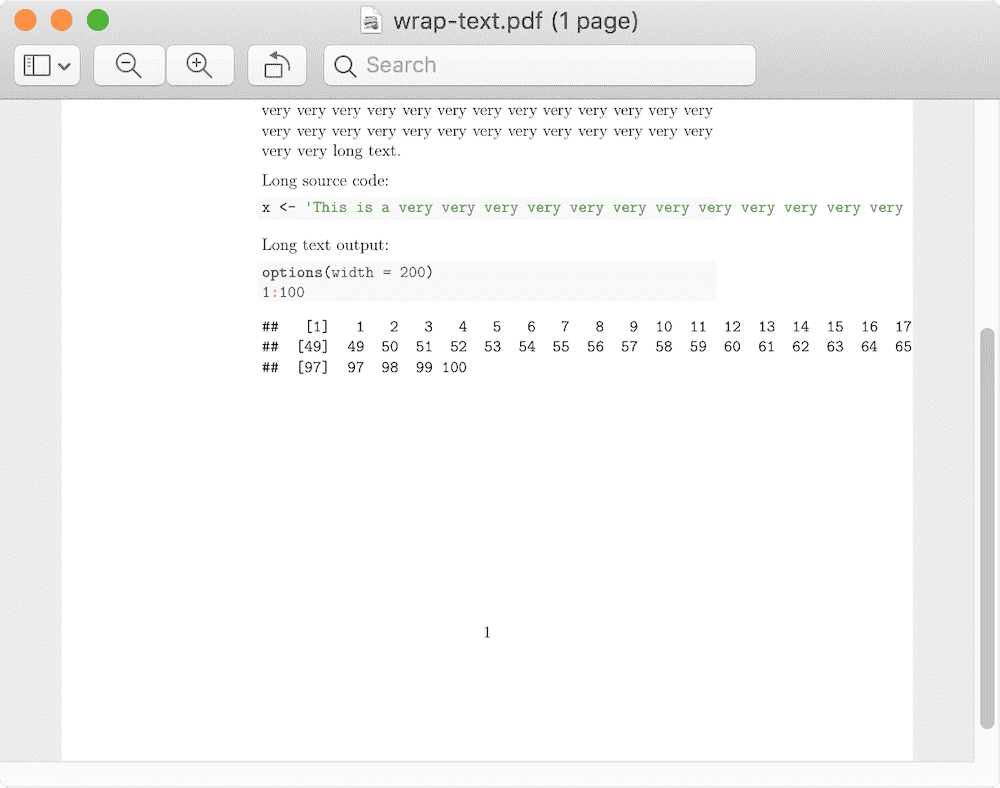
\includegraphics[width=1\linewidth,height=1\textheight,keepaspectratio]{JP/images/wrap-none} 

}

\caption{幅が広すぎる通常のテキスト出力}\label{fig:wrap-text-1}
\end{figure}
\begin{figure}

{\centering 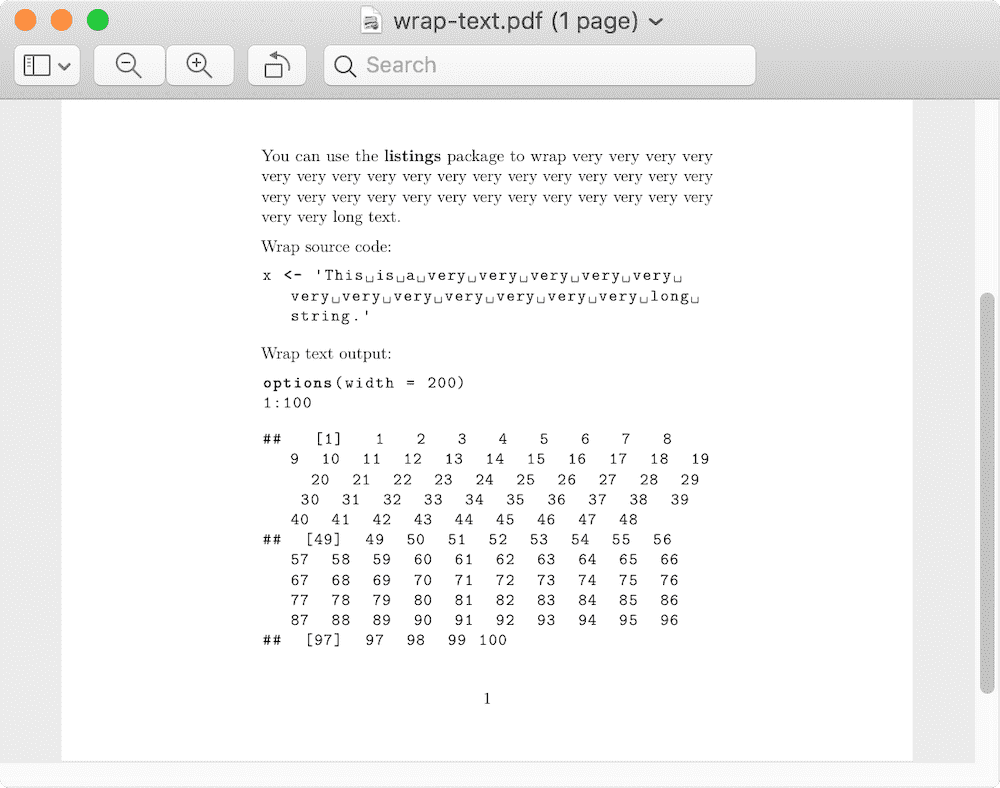
\includegraphics[width=1\linewidth,height=1\textheight,keepaspectratio]{JP/images/wrap-listings} 

}

\caption{listings パッケージで折り返されたテキスト出力}\label{fig:wrap-text-2}
\end{figure}

\textbf{訳注}: \textbf{listings} には多くのオプションがありますが, それだけでデフォルトのシンタックスハイライトを再現するのは難しいです. コードブロックの折返しは \textbf{knitr} の \texttt{styler} オプションである程度制御できます. Pandoc は出力ブロックをほとんど表示オプションのない \texttt{verbatim} 環境として出力し, これが問題の主な原因です. フィルタや LaTeX マクロを使うなどしてこの環境を置き換えればデフォルトのシンタックスハイライトと折返しを両立することができます.

\hypertarget{figure-size}{%
\section{グラフ・画像のサイズを制御する}\label{figure-size}}

R が作成するグラフのサイズ\index{図!サイズ}はチャンクオプション\texttt{fig.width} \index{チャンクオプション!fig.with} と \texttt{fig.height} \index{チャンクオプション!fig.height}でインチ単位で制御できます. 同様に \texttt{fig.dim} オプション \index{チャンクオプション!fig.dim}に長さ2のベクトルで幅と高さを指定できます. 例えば \texttt{fig.dim = c(8, 6)} は \texttt{fig.width = 8} と \texttt{fig.height = 6} を指定したのと同じです. これらのオプションはグラフの物理的なサイズを設定し, さらに \texttt{out.width}\index{チャンクオプション!out.width} と \texttt{out.height}\index{チャンクオプション!out.height}を使い出力時に異なるサイズで, 例えば \texttt{out.width = "50\%"} のように表示することが出来ます.

R コードチャンクで生成されないグラフや画像は, 2通りの方法で掲載できます.

\begin{itemize}
\item
  Markdown 構文 \texttt{!{[}キャプション{]}(画像ファイルパス)} を使う. この場合は \texttt{width}, \texttt{height} 属性でサイズを設定できます 例えばこのように.

\begin{Shaded}
\begin{Highlighting}[]
\NormalTok{次のパラグラフに画像を掲載する.}

\AlertTok{![良い画像](なんとか.png)}\NormalTok{\{width=50\%\}}
\end{Highlighting}
\end{Shaded}
\item
  コードチャンクで \textbf{knitr} 関数 \texttt{knitr::include\_graphics()}\index{knitr!include\_graphics()} を使う. そのチャンクで \texttt{out.width} と \texttt{out.height} といったオプションを設定することもできます. 例えばこのように.

\begin{Shaded}
\begin{Highlighting}[]
\NormalTok{R function を使って外部画像ファイルを掲載します}

\InformationTok{\textasciigrave{}\textasciigrave{}\textasciigrave{}\{r, echo=FALSE, out.width="50\%", fig.cap="良い画像"\}}
\InformationTok{knitr::include\_graphics("なんとか.png")}
\InformationTok{\textasciigrave{}\textasciigrave{}\textasciigrave{}}
\end{Highlighting}
\end{Shaded}
\end{itemize}

上記の例では幅 \texttt{50\%} が使われており, 画像コンテナの半分の幅にすることを意味します (もし画像がページの子要素ではなく, ページに直接含まれていると仮定すると, これはページ幅の半分を意味します). 特定の出力フォーマットに対してのみ画像を生成することが分かっているのなら, 単位を特定することもできます. たとえば出力フォーマットが HTML なら \texttt{300px} と書けるでしょう.

\hypertarget{fig-align}{%
\section{図のアラインメント}\label{fig-align}}

チャンクオプション \texttt{fig.align}\index{チャンクオプション!fig.align} は図のアラインメントを指定します. 例えば \texttt{fig.align = \textquotesingle{}center\textquotesingle{}} で中央揃え, あるいは \texttt{fig.align = \textquotesingle{}right\textquotesingle{}} で右揃えができます. このオプションは HTML と LaTeX 出力の両方で機能しますが, 他の出力フォーマット (残念ですが Word といったものは) では機能しないかもしれません. R コードチャンクで描画されたグラフも, \texttt{knitr::include\_graphics()}\index{knitr!include\_graphics()} で取り込まれた外部イメージに対しても機能します.

\hypertarget{verbatim-code-chunks}{%
\section{コードチャンクをそのまま (verbatim) 表示}\label{verbatim-code-chunks}}

典型的には私達はコードチャンクとインラインコードを \textbf{knitr} によってパースされ評価してほしいと思って書きますが, もし \textbf{knitr} を使ったチュートリアルを書きたいなら, \textbf{knitr} にパース\textbf{されない}コードチャンクやインラインコードを生成する必要があり, そしてチャンクヘッダの中身も掲載したいということもあるかもしれません.

不運なことにコードチャンクをさらに別のバッククオートのレイヤで囲むことは出来ませんが, 代わりにチャンクヘッダに \texttt{\textasciigrave{}r\ \textquotesingle{}\textquotesingle{}\textasciigrave{}}\index{knitr!inline\_expr()} を挿入することでソースコード内でコードチャンクを無効化しなければなりません. これは \textbf{knitr} によって, \textbf{空の文字列}のインラインコードであるものと評価されます. この例ではソース文書内の以下の「コードチャンク」

\begin{verbatim}
```{r, eval=TRUE}`r ''`
1 + 1
```
\end{verbatim}

は出力時にはこのようにレンダリングされます.

\begin{verbatim}
```{r, eval=TRUE}
1 + 1
```
\end{verbatim}

空の文字列で置き換えられるため, インラインコードは消え去ります. しかしこれは第1歩にすぎません. 出力時になんらかの無加工のコードを表示するには, Markdown の構文はコードブロックで包まれているべきです (スペース4つ分のインデントかバッククオートによる囲みで). 上記の出力を見たいとき, 実際のソースは以下のようになります.

\begin{verbatim}
````
```{r, eval=TRUE}`r ''`
1 + 1
```
````
\end{verbatim}

なぜバッククオートが4つなのでしょうか. これは N 個のバッククオートを包むには, 少なくとも N+1 個のバッククオートを使わなければならないからです.

\hypertarget{show-a-verbatim-inline-expression}{%
\subsection{インライン R コードをそのまま表示}\label{show-a-verbatim-inline-expression}}

行内のコードをそのまま表示する方法はいくつかあります. 最初の方法は \texttt{\textasciigrave{}r} の直後でインラインコードを改行することです. 例えばこのように.

\begin{Shaded}
\begin{Highlighting}[]
\NormalTok{これは出力時にインライン R コードをそのまま表示します \textasciigrave{}}\InformationTok{\textasciigrave{} \textasciigrave{}}\NormalTok{r}
\NormalTok{1+1\textasciigrave{} \textasciigrave{}\textasciigrave{}.}
\end{Highlighting}
\end{Shaded}

これが出力文書ではこうなっているはずです.

\begin{quote}
これは出力時にインライン R コードをそのまま表示します \texttt{\textasciigrave{}r\ 1+1\textasciigrave{}}.
\end{quote}

この小技は2つの理由で動作します. (1) Markdown パーサはしばしば単独の改行文字を単なるスペース1つとして扱う (2連続の改行は新しい段落を始めることと比べてみてください) ということと, (2) \textbf{knitr} は \texttt{\textasciigrave{}r} をパースするのに直後にスペース1つを要求する, つまりここにスペースがないとインラインコードとして扱われないということです.

インライン R コードをそのまま表示する別の方法は, R コードを \texttt{knitr::inline\_expr()} で包むことです. 例えばこのように.

\begin{Shaded}
\begin{Highlighting}[]
\NormalTok{これで出力時にインライン R コードがそのまま表示されます}
\InformationTok{\textasciigrave{}\textasciigrave{} \textasciigrave{}r knitr::inline\_expr("1+1")\textasciigrave{} \textasciigrave{}\textasciigrave{}}\NormalTok{.}
\end{Highlighting}
\end{Shaded}

私 (Yihui) は2つ目の方法をお薦めします. 1つ目の方法は多かれ少なかれ Markdown 構文と \textbf{knitr} パーサに対するハック的なものだからです.

\hypertarget{number-lines}{%
\section{コードブロックに行番号を表示する (*)}\label{number-lines}}

\texttt{attr.source = ".numberLines"}\index{チャンクオプション!attr.source} でソースコードブロックにも行番号を付けることも, \texttt{attr.output = ".numberLines"}\index{チャンクオプション!attr.output} でテキスト出力ブロックに行番号を付けることもできます (これらのオプションの詳細は\ref{attr-output}節参照). 例えばこのように.

\begin{Shaded}
\begin{Highlighting}[]
\InformationTok{\textasciigrave{}\textasciigrave{}\textasciigrave{}\{r, attr.source=\textquotesingle{}.numberLines\textquotesingle{}\}}
\InformationTok{if (TRUE) \{}
\InformationTok{  x \textless{}{-} 1:10}
\InformationTok{  x + 1}
\InformationTok{\}}
\InformationTok{\textasciigrave{}\textasciigrave{}\textasciigrave{}}
\end{Highlighting}
\end{Shaded}

出力はこうなります.

\begin{Shaded}
\begin{Highlighting}[numbers=left,,]
\ControlFlowTok{if}\NormalTok{ (}\ConstantTok{TRUE}\NormalTok{) \{}
\NormalTok{  x }\OtherTok{\textless{}{-}} \DecValTok{1}\SpecialCharTok{:}\DecValTok{10}
\NormalTok{  x }\SpecialCharTok{+} \DecValTok{1}
\NormalTok{\}}
\end{Highlighting}
\end{Shaded}

HTML 出力では, Pandoc が提供するシンタックスハイライト\index{シンタックスハイライト} のテーマ\index{出力オプション!highlight} を選ぶ必要があることに注意してください. これは出力フォーマットの \texttt{highlight} オプションを \texttt{default} や \texttt{textmate} にすべきではないということを意味します. ヘルプページ \texttt{?rmarkdown::html\_document} でこのオプションの他の値の一覧を見ることができます. 例えばこう設定できます.

\begin{Shaded}
\begin{Highlighting}[]
\FunctionTok{output}\KeywordTok{:}
\AttributeTok{  }\FunctionTok{html\_document}\KeywordTok{:}
\AttributeTok{    }\FunctionTok{highlight}\KeywordTok{:}\AttributeTok{ tango}
\end{Highlighting}
\end{Shaded}

\textbf{bookdown} の \texttt{gitbook} 出力フォーマットでは, コードの左側の適切な位置に数字を表示するために CSS を多少調整する必要があるかもしれません. 以下は本書で使用しているものです (行番号がページ左余白に近すぎると思ったら, \texttt{left} の値を \texttt{-0.2em} などに増やして調整してください).\footnote{\textbf{訳注}: 日本語版は \textbf{rmdja} の出力フォーマットを使用しており, これはデフォルトで行番号を表示し, かつ gitbook に対応した調整を予め搭載しています.}

\begin{Shaded}
\begin{Highlighting}[]
\NormalTok{pre}\FunctionTok{.numberSource}\NormalTok{ code }\OperatorTok{\textgreater{}}\NormalTok{ span }\OperatorTok{\textgreater{}}\NormalTok{ a}\InformationTok{:first{-}child::before}\NormalTok{ \{}
  \KeywordTok{left}\NormalTok{: }\DecValTok{{-}0.3}\DataTypeTok{em}\OperatorTok{;}
\NormalTok{\}}
\end{Highlighting}
\end{Shaded}

\textbf{revealjs} の \texttt{revealjs\_presentation} 出力フォーマット \autocite{R-revealjs} に対しても CSS の調整が必要かもしれません.

\begin{Shaded}
\begin{Highlighting}[]
\FunctionTok{.reveal}\NormalTok{ pre code \{}
  \KeywordTok{overflow}\NormalTok{: }\DecValTok{visible}\OperatorTok{;}
\NormalTok{\}}
\end{Highlighting}
\end{Shaded}

カスタム CSS スタイルを HTML 出力に適用する方法がわからないなら, \ref{html-css}節を見てください.

\texttt{startFrom} 属性で開始する数字を指定することもできます. 例えばこのように.

\begin{Shaded}
\begin{Highlighting}[]
\InformationTok{\textasciigrave{}\textasciigrave{}\textasciigrave{}\{r, attr.source=\textquotesingle{}.numberLines startFrom="5"\textquotesingle{}\}}
\InformationTok{if (TRUE) \{}
\InformationTok{  1:10}
\InformationTok{\}}
\InformationTok{\textasciigrave{}\textasciigrave{}\textasciigrave{}}
\end{Highlighting}
\end{Shaded}

現時点では Word 出力での行番号はサポートしていません.

\hypertarget{multi-column}{%
\section{多段組み (*)}\label{multi-column}}

Pandoc の Markdown はスライドに対する多段レイアウトをサポートしていますが, 他のタイプの文書ではサポートしていません. このレシピでは通常の HTML 文書や LaTeX 文書での多段レイアウトを使う方法を紹介します. これは \textbf{knitr} の issue \url{https://github.com/yihui/knitr/issues/1743} での Atsushi Yasumoto の解決策に着想を得ました.

HTML 要素を CSS\index{CSS} を使って並べて表示するのは比較的簡単なので, この方法は HTML 出力のみ考慮する必要があるならかなり簡単です. コードチャンクのテキスト出力を並べるだけならば, もっと簡単になります. 以下は1つ目の例です.

\begin{Shaded}
\begin{Highlighting}[]
\CommentTok{{-}{-}{-}}
\AnnotationTok{output:}\CommentTok{ html\_document}
\CommentTok{{-}{-}{-}}

\InformationTok{\textasciigrave{}\textasciigrave{}\textasciigrave{}\{r attr.source="style=\textquotesingle{}display:inline{-}block;\textquotesingle{}", collapse=TRUE\}}
\InformationTok{1:10  \# 1 から 10 の数列}
\InformationTok{10:1  \# その逆順}
\InformationTok{\textasciigrave{}\textasciigrave{}\textasciigrave{}}
\end{Highlighting}
\end{Shaded}

CSS 属性 \texttt{display: inline-block;} \index{CSS プロパティ!display} はコードブロックの出力 (つまり HTML タグの \texttt{\textless{}pre\textgreater{}} です) をインライン要素として表示すべきという意味です. デフォルトではこれらのブロックはブロックレベル要素 (つまり \texttt{display: block;}) として表示され, 行を丸ごと占有します. チャンクオプション \texttt{collapse = TRUE} はテキスト出力を R ソースコードブロックと結合することを意味するので, ソースとテキスト出力が同じ \texttt{\textless{}pre\textgreater{}} ブロックに配置されます.

HTML 出力時に任意の順で横に並べたい場合, Pandoc の \href{https://pandoc.org/MANUAL.html\#divs-and-spans}{fenced \texttt{Div}.}\index{Div}\index{Pandoc!Div| see {Div}} を使うことができます. ``Div'' は HTML タグの \texttt{\textless{}div\textgreater{}} に由来しますが, 任意のブロックやコンテナと解釈できます. \texttt{Div} の開始と終了は は3つ以上のコロン (例: \texttt{:::}) です. より多くのコロンの \texttt{Div} は, よりコロンの少ない \texttt{Div} を含むことができます. fanced \texttt{Div} の重要で有用な機能は, これに属性を付与できるということです. 例えば CSS 属性 \texttt{display: flex;} を外側のコンテナに適用できるので, 内側のコンテナは横並びに配置されます.

\begin{Shaded}
\begin{Highlighting}[]
\CommentTok{{-}{-}{-}}
\AnnotationTok{output:}\CommentTok{ html\_document}
\CommentTok{{-}{-}{-}}

\NormalTok{:::: \{style="display: flex;"\}}

\NormalTok{::: \{\}}
\NormalTok{ここは **最初の** Div です.}

\InformationTok{\textasciigrave{}\textasciigrave{}\textasciigrave{}\{r\}}
\InformationTok{str(iris)}
\InformationTok{\textasciigrave{}\textasciigrave{}\textasciigrave{}}
\NormalTok{:::}

\NormalTok{::: \{\}}
\NormalTok{こっちは右側に配置されるブロックです.}

\InformationTok{\textasciigrave{}\textasciigrave{}\textasciigrave{}\{r\}}
\InformationTok{plot(iris[, {-}5])}
\InformationTok{\textasciigrave{}\textasciigrave{}\textasciigrave{}}
\NormalTok{:::}

\NormalTok{::::}
\end{Highlighting}
\end{Shaded}

上記の例では外側の \texttt{Div} (\texttt{::::}) は2つの \texttt{Div} (\texttt{:::}) を含んでいます. この中にさらに \texttt{Div} を追加することもできます. とても強力な CSS 属性 \texttt{display: flex;} (CSS Flexbox) についてもっと知るためには \url{https://css-tricks.com/snippets/css/a-guide-to-flexbox/} というガイドを読むこともできます. CSS グリッド (\texttt{display: grid;}) はもっと強力で, 上記の例にも使えます. もし試してみたいなら, \texttt{display: flex;} を \texttt{display: grid; grid-template-columns: 1fr 1fr; grid-column-gap: 10px;} に置き換えてみてください. グリッドレイアウトについてより知りたいのなら, \url{https://css-tricks.com/snippets/css/complete-guide-grid/} のガイドを見てください.

HTML でも LaTeX でも同じようなレイアウトにしたいのなら, よりトリッキーになります. 以下に HTML, LaTeX そして Beamer で動作する用例の全容を示します.

\begin{Shaded}
\begin{Highlighting}[]
\CommentTok{{-}{-}{-}}
\AnnotationTok{output:}
\CommentTok{  pdf\_document: }
\CommentTok{    latex\_engine: lualatex}
\CommentTok{    keep\_tex: true}
\CommentTok{    includes:}
\CommentTok{      in\_header: columns.tex}
\CommentTok{  html\_document: }
\CommentTok{    css: columns.css}
\CommentTok{  beamer\_presentation: }
\CommentTok{    keep\_tex: true}
\CommentTok{    latex\_engine: lualatex}
\CommentTok{    includes:}
\CommentTok{      in\_header: columns.tex}
\AnnotationTok{documentclass:}\CommentTok{ "\textasciigrave{}r if(knitr::opts\_knit$get(\textquotesingle{}rmarkdown.pandoc.to\textquotesingle{}) == \textquotesingle{}beamer\textquotesingle{}) \textquotesingle{}beamer\textquotesingle{} else \textquotesingle{}ltjsarticle\textquotesingle{}\textasciigrave{}"}
\AnnotationTok{mainfont:}\CommentTok{ \textquotesingle{}Noto Sans CJK JP\textquotesingle{}}
\CommentTok{{-}{-}{-}}

\FunctionTok{\# 二段組み}

\NormalTok{以下は 3つの子要素の Div を横並びに持つ Div コンテナです. 中央の Div は空で, 左右の Div の間に空白を作るためだけに存在します.}

\NormalTok{:::::: \{.cols data{-}latex=""\}}

\NormalTok{::: \{.col data{-}latex="\{0.55\textbackslash{}textwidth\}"\}}
\InformationTok{\textasciigrave{}\textasciigrave{}\textasciigrave{}\{r, echo=FALSE, fig.width=5, fig.height=4\}}
\InformationTok{par(mar = c(4, 4, .2, .1))}
\InformationTok{plot(cars, pch = 19)}
\InformationTok{\textasciigrave{}\textasciigrave{}\textasciigrave{}}
\NormalTok{:::}

\NormalTok{::: \{.col data{-}latex="\{0.05\textbackslash{}textwidth\}"\}}
\NormalTok{\textbackslash{} }
\CommentTok{\textless{}!{-}{-} 段どうしのセパレータとして機能するだけの空の Div (空白入り) {-}{-}\textgreater{}}
\NormalTok{:::}

\NormalTok{::: \{.col data{-}latex="\{0.4\textbackslash{}textwidth\}"\}}
\NormalTok{左側の図は }\InformationTok{\textasciigrave{}cars\textasciigrave{}}\NormalTok{ データを表しています.}


\AttributeTok{\textgreater{} いろはにほへと ちりぬるを}
\AttributeTok{わかよたれそ つねならむ}
\AttributeTok{うゐのおくやま けふこえて}
\AttributeTok{あさきゆめみし ゑひもせす}

\NormalTok{:::}
\NormalTok{::::::}
\end{Highlighting}
\end{Shaded}

\begin{figure}

{\centering 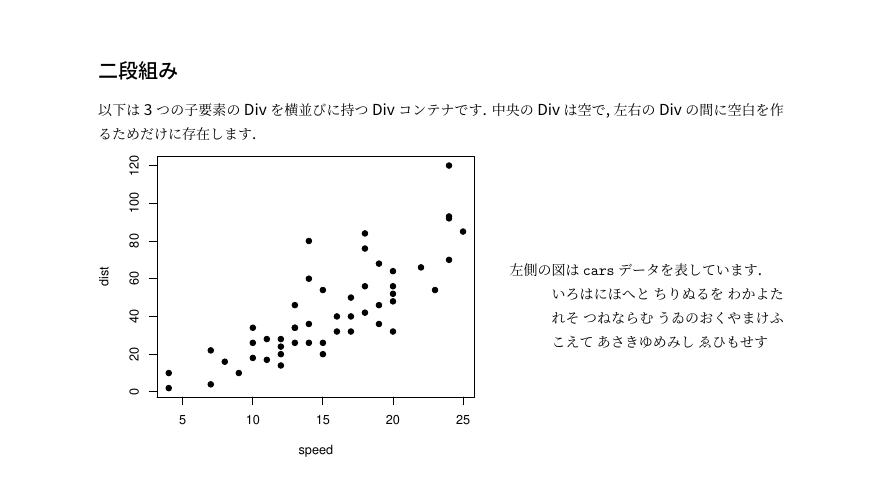
\includegraphics[width=1\linewidth,height=1\textheight,keepaspectratio]{JP/images/multicol} 

}

\caption{HTML, LaTeX, Beamer で動作する二段組み}\label{fig:multicol}
\end{figure}

図\ref{fig:multicol} がその出力です. この例では外側の \texttt{.cols} クラスを持つ \texttt{Div} と, 内側に \texttt{.col} クラスを持つ3つの \texttt{Div} を使っています. HTML 出力では, 外部 CSS ファイル \texttt{columns.css} を導入し, その中で Flexbox レイアウトを外側の \texttt{Div} に適用しているので, 内側の \texttt{Div} が横並びになります.

\begin{Shaded}
\begin{Highlighting}[]
\FunctionTok{.cols}\NormalTok{ \{}\KeywordTok{display}\NormalTok{: flex}\OperatorTok{;}\NormalTok{ \}}
\end{Highlighting}
\end{Shaded}

LaTeX 出力 (\texttt{pdf\_document}) では, LaTeX プリアンブルで LaTeX 環境 \texttt{cols} と \texttt{col} で定義するための \texttt{columns.tex} に含まれているダーティーハックについて解説せねばなりません.

\begin{Shaded}
\begin{Highlighting}[]
\FunctionTok{\textbackslash{}newenvironment}\NormalTok{\{cols\}[1][]\{\}\{\}}

\FunctionTok{\textbackslash{}newenvironment}\NormalTok{\{col\}[1]\{}\KeywordTok{\textbackslash{}begin}\NormalTok{\{}\ExtensionTok{minipage}\NormalTok{\}\{\#1\}}\FunctionTok{\textbackslash{}ignorespaces}\NormalTok{\}\{}\CommentTok{\%}
\KeywordTok{\textbackslash{}end}\NormalTok{\{}\ExtensionTok{minipage}\NormalTok{\}}
\FunctionTok{\textbackslash{}ifhmode\textbackslash{}unskip\textbackslash{}fi}
\FunctionTok{\textbackslash{}aftergroup\textbackslash{}useignorespacesandallpars}\NormalTok{\}}

\FunctionTok{\textbackslash{}def\textbackslash{}useignorespacesandallpars}\NormalTok{\#1}\FunctionTok{\textbackslash{}ignorespaces\textbackslash{}fi}\NormalTok{\{}\CommentTok{\%}
\NormalTok{\#1}\FunctionTok{\textbackslash{}fi\textbackslash{}ignorespacesandallpars}\NormalTok{\}}

\FunctionTok{\textbackslash{}makeatletter}
\FunctionTok{\textbackslash{}def\textbackslash{}ignorespacesandallpars}\NormalTok{\{}\CommentTok{\%}
  \FunctionTok{\textbackslash{}@ifnextchar\textbackslash{}par}
\NormalTok{    \{}\FunctionTok{\textbackslash{}expandafter\textbackslash{}ignorespacesandallpars\textbackslash{}@gobble}\NormalTok{\}}\CommentTok{\%}
\NormalTok{    \{\}}\CommentTok{\%}
\NormalTok{\}}
\FunctionTok{\textbackslash{}makeatother}
\end{Highlighting}
\end{Shaded}

主に Pandoc が LaTeX 出力では \texttt{Div} に対していつも段落を改めており, この改段を除去しなければならないという理由のため, \texttt{col} 環境は特に複雑です. そうしないと \texttt{Div} を横並びにすることはできません. このハックは \url{https://tex.stackexchange.com/q/179016/9128} から借用しました.

Beamer 出力でも \texttt{columns.tex} で同じハックを適用しています. Pandoc は \texttt{::: \{.columns\}}, \texttt{::: \{.column\}}, \texttt{::: \{.incremental\}} といった\href{https://pandoc.org/MANUAL.html\#producing-slide-shows-with-pandoc}{スライドショー}用の特別な \texttt{Div} を提供していることに注意してください. これらは特別な意味を持つため, この節で言及されたような方法で \texttt{Div} を LaTeX 環境を変換しようとするなら, これらのタイプの \texttt{Div} を\textbf{使わない}ように注意しなければなりません. \texttt{columns} または \texttt{column} ではなく, \texttt{cols}, \texttt{col} という名前の \texttt{Div} タイプを使ったのはこれが理由です.

fenced \texttt{Div} についてより詳しく知りたいなら, \ref{custom-blocks}節を見てください.

\textbf{訳注}: 二段組にしたいのが PDF 限定であれば, YAML フロントマターのみで簡単に制御することができます (\ref{latex-variables}節参照).

\hypertarget{latex-output}{%
\chapter{LaTeX 出力}\label{latex-output}}

多くの著者にとって作品の主な出力は PDF レポートで, この出力では強力な LaTex のスタイル設定を活用できます. この章では, LaTeX コードやパッケージをプリアンブルに含めることや, カスタム LaTeX レンプレートの使用, ヘッダとフッタの追加, 図を分割して生成する方法, 生の LaTeX コードを文書の本文に書く方法, といったPDFレポートのカスタマイズに使えるアプローチについて議論します.

ただし, 始める前に注意しておきたいことがあります.R Markdown の恩恵の1つは単一のソース文書から複数のフォーマットの文書を生成できるということです. あなたの作品を単一の出力に対して仕立て上げるこにとよって, その出力フォーマット単体の見た目やパフォーマンスは向上するかもしれませんが, それはこの移植性を犠牲にすることでもあります. この問題は LaTeX に限ったことでなく. 他の出力フォーマットでも同様です.

\hypertarget{latex-preamble}{%
\section{プリアンブルに LaTeX コードを追加する}\label{latex-preamble}}

LaTeX 文書\index{LaTeX}の一般的な構造はこのようになっています.

\begin{Shaded}
\begin{Highlighting}[]
\BuiltInTok{\textbackslash{}documentclass}\NormalTok{\{}\ExtensionTok{article}\NormalTok{\}}
\CommentTok{\% preamble}
\KeywordTok{\textbackslash{}begin}\NormalTok{\{}\ExtensionTok{document}\NormalTok{\}}
\CommentTok{\% body}
\KeywordTok{\textbackslash{}end}\NormalTok{\{}\ExtensionTok{document}\NormalTok{\}}
\end{Highlighting}
\end{Shaded}

これは文書クラスを \texttt{\textbackslash{}documentclass\{\}} で宣言し, 必要に応じて特定の LaTeX パッケージを読み込んだり特定のオプションをプリアンブルで設定し, そして \texttt{\textbackslash{}begin\{document\}} の後で文書の本文を書き始めています. Markdown 文書はほとんどがこの文書の本文に対応します.

プリアンブルになにか追加したい時, \texttt{pdf\_document}\index{出力オプション!includes} \texttt{include} を使わねばなりません. このオプションは3つのサブオプションを持ちます. \texttt{in\_header}, \texttt{before\_body}, そして \texttt{after\_body} です. これらは1つ以上のファイルパスを指定できます. \texttt{in\_header} に指定されたファイルはプリアンブルに追加されます. \texttt{before\_body} と \texttt{after\_body} に指定されたファイルはそれぞれ本文の前と後に追加されます.

例えば以下はテキスト内のハイパーリンクを脚注に変えるトリックです. PDF 出力された文書が紙に印刷されたものだと, 読者は紙面のリンク (\texttt{\textbackslash{}href\{URL\}\{text\}} で生成されたもの) をクリックすることはできませんが, 脚注の URL を見ることはできるのでこのトリックは役に立ちます. このトリックはテキストと URL の両方を表示します.

\begin{Shaded}
\begin{Highlighting}[]
\CommentTok{\% あなたはレンダリング前に \textbackslash{}href のコピーを保存したいかもしれない}
\CommentTok{\% \textbackslash{}let\textbackslash{}oldhref\textbackslash{}href}
\FunctionTok{\textbackslash{}renewcommand}\NormalTok{\{}\ExtensionTok{\textbackslash{}href}\NormalTok{\}[2]\{\#2}\FunctionTok{\textbackslash{}footnote}\NormalTok{\{}\FunctionTok{\textbackslash{}url}\NormalTok{\{\#1\}\}\}}
\end{Highlighting}
\end{Shaded}

あるファイル名 , 例えば \texttt{preamble.tex} 内に上記のコードを保存できます. それからプリアンブルにこれを読み込んでください.

\begin{Shaded}
\begin{Highlighting}[]
\FunctionTok{output}\KeywordTok{:}
\AttributeTok{  }\FunctionTok{pdf\_document}\KeywordTok{:}
\AttributeTok{    }\FunctionTok{includes}\KeywordTok{:}
\AttributeTok{      }\FunctionTok{in\_header}\KeywordTok{:}\AttributeTok{ }\StringTok{"preamble.tex"}
\end{Highlighting}
\end{Shaded}

このトリックは実際には自分で実装しなくてもよく, Pandoc のデフォルトのテンプレート (\ref{latex-variables}節参照) に組み込まれた機能である YAML オプション \texttt{links-as-notes} を `true``\index{YAML!links-as-notes}にすることで簡単にできます.

コードをプリアンブルに追加する別の方法は, YAML フロントマター\index{YAML!header-includes} の \texttt{header-includes} フィールドに直接与えることです. \ref{latex-logo}節でその例を紹介しています. \texttt{header-includes} を使う利点は R Markdown 文書1つの内部に全てを含められることです. しかしあなたのレポートを複数の出力フォーマットに生成しなければならないなら, \texttt{includes} を使う方法をお薦めします. \texttt{header-includes} は無条件であり, 非 LaTeX 出力の文書に対しても読み込まれてしまうからです. 比較として, \texttt{includes} オプションは \texttt{pdf\_document} フォーマットにのみ適用されます.

\hypertarget{latex-variables}{%
\section{LaTeX 出力の Pandoc オプション}\label{latex-variables}}

LaTeX 出力に対してデフォルトの Pandoc を使うなら, PDF 出力の文書の見た目を調整するいくつかのオプションがあります. いくつかのオプションの例を以下に挙げていきます. 完全なリストは \url{https://pandoc.org/MANUAL.html\#variables-for-latex} で見ることができます.

\begin{Shaded}
\begin{Highlighting}[]
\FunctionTok{documentclass}\KeywordTok{:}\AttributeTok{ book}
\FunctionTok{classoption}\KeywordTok{:}
\AttributeTok{  }\KeywordTok{{-}}\AttributeTok{ twocolumn}
\AttributeTok{  }\KeywordTok{{-}}\AttributeTok{ landscape}
\FunctionTok{papersize}\KeywordTok{:}\AttributeTok{ a5}
\FunctionTok{linestretch}\KeywordTok{:}\AttributeTok{ }\FloatTok{1.5}
\FunctionTok{fontsize}\KeywordTok{:}\AttributeTok{ 12pt}
\FunctionTok{links{-}as{-}notes}\KeywordTok{:}\AttributeTok{ }\CharTok{true}
\end{Highlighting}
\end{Shaded}

あなたが LaTeX にある程度詳しいなら, これらのオプションの意味は明らかでしょう. \texttt{documentclass} オプション\index{YAML!documentclass} は, 例えば \texttt{article}, \texttt{book}, \texttt{report} などの文書クラスを設定します. \texttt{classoption} は文書クラスに与えるオプションのリストで, 例えば二段組の文書を作りたいなら \texttt{twocolumn} オプション,\footnote{このオプションは文書全体を変更しますが, 特定の位置から再度一段組に戻したいのなら, そこに \texttt{\textbackslash{}onecolumn} コマンドを挿入することになるでしょう. 二段組モードを続けたいなら \texttt{\textbackslash{}twocolumn} を挿入します.}, 横置きレイアウトにするなら \texttt{landscape} オプション (デフォルトでは縦置き (portrait) レイアウト) があります. \texttt{papersize}\index{YAML!papersize} オプションは \texttt{a4}, \texttt{paper}, \texttt{a5} といった用紙サイズを設定します. \texttt{linestretch}\index{YAML!linestretch} オプションは行間を設定します. \texttt{fontsize}\index{YAML!fontsize} オプションはフォントサイズを \texttt{10pt}, \texttt{11pt}, \texttt{12pt} というふうに設定します. \texttt{links-as-notes} オプションはテキスト内のリンクを脚注に置き換えます. 紙に印刷する際には読者は紙面上のリンクをクリックできませんが, 脚注の URL を見ることができるので便利です.

フォントの変更は少しトリッキーです. どの LaTeX エンジンを使っているかに依存します. LaTeX ベースの出力フォーマットで大抵の場合デフォルトである \texttt{pdflatex}\index{pdflatex} を使っているのなら\footnote{\textbf{訳注}: 日本語文書を \textbf{pdflatex} で出力することは全く不可能というわけではありませんが, 技術的制約が多いため LaTeX に慣れている方以外にはお薦めしません.}, 読み込む LaTeX フォントパッケージを選択するために \texttt{fontfamily} オプションを使ってください. 例えばこのように.

\begin{Shaded}
\begin{Highlighting}[]
\FunctionTok{fontfamily}\KeywordTok{:}\AttributeTok{ accanthis}
\FunctionTok{output}\KeywordTok{:}
\AttributeTok{  }\FunctionTok{pdf\_document}\KeywordTok{:}\AttributeTok{ }
\AttributeTok{    }\FunctionTok{latex\_engine}\KeywordTok{:}\AttributeTok{ pdflatex}
\end{Highlighting}
\end{Shaded}

これで文書に \href{https://tug.org/FontCatalogue/accanthis/}{Accanthis} フォントが使われます. 他の多数の LaTeX フォントパッケージのリストは You may see \url{https://tug.org/FontCatalogue/} で見ることができます. LaTeX ディストリビューションに TinyTeX をお使いで, フォントパッケージがインストールされていないならば, 文書がコンパイルされる際に自動でインストールされるはずです(\ref{install-latex}節参照).

LaTeX エンジンに \texttt{xelatex} または \texttt{lualatex} を使っているなら, ローカルのコンピュータで使用可能なフォントから選ぶことができ, LaTeX パッケージの追加インストールはしなくともよいです. YAML オプション \texttt{mainfont}\index{YAML!mainfont}, \texttt{sansfont}\index{YAML!sansfont}, \texttt{monofont}\index{YAML!monofont} はメインのフォント, サンセリフ体, そしてタイプライタ体のフォントをそれぞれ指定するのに使えます.\footnote{\textbf{訳注}: rmdja では YAML フロントマターでさらに欧文用フォントと和文用フォントを個別に指定できます.} 例えばこのように.

\begin{Shaded}
\begin{Highlighting}[]
\FunctionTok{mainfont}\KeywordTok{:}\AttributeTok{ Arial}
\FunctionTok{output}\KeywordTok{:}
\AttributeTok{  }\FunctionTok{pdf\_document}\KeywordTok{:}\AttributeTok{ }
\AttributeTok{    }\FunctionTok{latex\_engine}\KeywordTok{:}\AttributeTok{ xelatex}
\end{Highlighting}
\end{Shaded}

Beamer \index{Beamer}の文書は LaTeX 文書なので, Beamer でスライドを生成する時にもこれらのオプションを使用できます. 加えて, Pandoc は Beamer スライド用にいくつか追加オプションを提供してくれています. それらは \url{https://pandoc.org/MANUAL.html\#variables-for-beamer-slides} で確認できます. 例えば \texttt{institute} オプション\index{YAML!institute}で著者の所属機関を指定することができます.

\begin{Shaded}
\begin{Highlighting}[]
\PreprocessorTok{{-}{-}{-}}
\FunctionTok{output}\KeywordTok{:}\AttributeTok{ beamer\_presentation}
\FunctionTok{institute}\KeywordTok{:}\AttributeTok{ }\StringTok{"ハッカーの大学"}
\PreprocessorTok{{-}{-}{-}}
\end{Highlighting}
\end{Shaded}

\hypertarget{latex-logo}{%
\section{表紙ページにロゴを置く}\label{latex-logo}}

LaTeX パッケージの \textbf{titling} \index{LaTeX パッケージ!titling} を表題ブロックを画像に変更\index{図!表紙ページ}するのに使うとができます. 以下は R ロゴ (\texttt{logo.jpg}) を表紙に配置する方法の例の全容です. 画像は LaTeX のサポートする形式 (例えば \texttt{jpg}, \texttt{png}, \texttt{pdf}) ならなんでも使えます.

\begin{Shaded}
\begin{Highlighting}[]
\CommentTok{{-}{-}{-}}
\AnnotationTok{title:}\CommentTok{ LaTeX のタイトルにロゴを追加する}
\AnnotationTok{author:}\CommentTok{ Michael Harper}
\AnnotationTok{date:}\CommentTok{ 2018/12/7}
\AnnotationTok{output:}
\CommentTok{  pdf\_document:}
\CommentTok{    latex\_engine: lualatex}
\AnnotationTok{documentclass:}\CommentTok{ ltjsarticle}
\AnnotationTok{header{-}includes:}
\CommentTok{  {-} \textbackslash{}usepackage\{titling\}}
\CommentTok{  {-} \textbackslash{}pretitle\{\textbackslash{}begin\{center\}}
\CommentTok{    \textbackslash{}includegraphics[width=2in,height=2in]\{logo.jpg\}\textbackslash{}LARGE\textbackslash{}\textbackslash{}\}}
\CommentTok{  {-} \textbackslash{}posttitle\{\textbackslash{}end\{center\}\}}
\CommentTok{{-}{-}{-}}

\CommentTok{\textless{}!{-}{-} 改ページを含めることもできます. これで文書を強制的に2ページ目から始めさせます. {-}{-}\textgreater{}}

\NormalTok{\textbackslash{}newpage}

\NormalTok{ここからあなたのレポート}

\InformationTok{\textasciigrave{}\textasciigrave{}\textasciigrave{}\{r, include=FALSE\}}
\InformationTok{\# R ロゴをカレントディレクトリにコピー}
\InformationTok{file.copy(file.path(R.home("doc"), "html", "logo.jpg"), \textquotesingle{}.\textquotesingle{})}
\InformationTok{\textasciigrave{}\textasciigrave{}\textasciigrave{}}
\end{Highlighting}
\end{Shaded}

図\ref{fig:latex-logo} がこの例の出力です.

\begin{figure}

{\centering 
\includegraphics[width=1\linewidth,height=1\textheight,keepaspectratio]{JP/images/latex-logo} 

}

\caption{LaTeX の表紙ページにロゴを追加する}\label{fig:latex-logo}
\end{figure}

LaTeX パッケージ (\textbf{titling}) を特に要求しない代替方法として, Markdown 構文を使って \texttt{title} フィールド\index{YAML!title}に画像を挿入する方法があります. 例えばこのように.

\begin{Shaded}
\begin{Highlighting}[]
\FunctionTok{title}\KeywordTok{: }\CharTok{|}
\NormalTok{  ![](logo.jpg)\{width=1in\}  }
\NormalTok{  LaTeX のタイトルにロゴを追加する}
\end{Highlighting}
\end{Shaded}

この場合, 最初の例のように YAML フロントマターの \texttt{header-includes} フィールドは不要になります. 例からは見えませんが, \texttt{!{[}{]}(logo.jpg)\{width=1in\}} の末尾にスペースが2つあることに注意してください. これは Markdown では改行を意味します(\ref{linebreaks}節参照). 改行がない場合画像とタイトルは同じ行に現れてしまい, きっとそれはあなたの意図するものではないでしょう.

\hypertarget{latex-extra}{%
\section{LaTeX パッケージを追加で読み込む}\label{latex-extra}}

追加の LaTeX パッケージ を使うことで文書のスタイルに拡張的なカスタマイズが可能になります. 加えて \textbf{kableExtra}\index{R パッケージ!kableExtra} \autocite{R-kableExtra} のようないくつかのパッケージは R パッケージの関数を提供するために LaTeX に依存しているかもしれません. R でもよくあるように, これらの関数を使えるようになる前に R Markdown 文書内でパッケージを読み込む必要があります.

\hypertarget{loading-latex-packages}{%
\subsection{LaTeX パッケージを読み込む}\label{loading-latex-packages}}

\texttt{pdf\_document} の YAML での設定 \texttt{extra\_dependencies} オプション\index{出力オプション!extra\_dependencies} を使って追加の LaTeX パッケージを読み込めます. 中間ファイルの LaTeX 出力文書で読み込む LaTeX パッケージ\index{LaTeX パッケージ}のリストを与えることができます. 例えばこのように.

\begin{Shaded}
\begin{Highlighting}[]
\PreprocessorTok{{-}{-}{-}}
\FunctionTok{title}\KeywordTok{:}\AttributeTok{ }\StringTok{"追加 LaTeX パッケージを使う"}
\FunctionTok{output}\KeywordTok{:}\AttributeTok{ }
\AttributeTok{  }\FunctionTok{pdf\_document}\KeywordTok{:}
\AttributeTok{    }\FunctionTok{extra\_dependencies}\KeywordTok{:}\AttributeTok{ }\KeywordTok{[}\StringTok{"bbm"}\KeywordTok{,}\AttributeTok{ }\StringTok{"threeparttable"}\KeywordTok{]}
\PreprocessorTok{{-}{-}{-}}
\end{Highlighting}
\end{Shaded}

パッケージ読み込み時のオプションを指定する必要があるなら, 第2のレベルを加えてオプションをリストとして与えられます. 例えばこのように.

\begin{Shaded}
\begin{Highlighting}[]
\FunctionTok{output}\KeywordTok{:}\AttributeTok{ }
\AttributeTok{  }\FunctionTok{pdf\_document}\KeywordTok{:}
\AttributeTok{    }\FunctionTok{extra\_dependencies}\KeywordTok{:}
\AttributeTok{      }\FunctionTok{caption}\KeywordTok{:}\AttributeTok{ }\KeywordTok{[}\StringTok{"labelfont=\{bf\}"}\KeywordTok{]}
\AttributeTok{      }\FunctionTok{hyperref}\KeywordTok{:}\AttributeTok{ }\KeywordTok{[}\StringTok{"unicode=true"}\KeywordTok{,}\AttributeTok{ }\StringTok{"breaklinks=true"}\KeywordTok{]}
\AttributeTok{      }\FunctionTok{lmodern}\KeywordTok{:}\AttributeTok{ }\CharTok{null}
\end{Highlighting}
\end{Shaded}

LaTeX に慣れた人にとっては, これは以下の LaTeX コードと同じです.

\begin{Shaded}
\begin{Highlighting}[]
\BuiltInTok{\textbackslash{}usepackage}\NormalTok{[labelfont=\{bf\}]\{}\ExtensionTok{caption}\NormalTok{\} }
\BuiltInTok{\textbackslash{}usepackage}\NormalTok{[unicode=true, breaklinks=true]\{}\ExtensionTok{hyperref}\NormalTok{\}}
\FunctionTok{\textbackslash{}userpackage}\NormalTok{\{lmodern\}}
\end{Highlighting}
\end{Shaded}

\ref{latex-preamble}節で紹介した \texttt{includes} 引数に対し \texttt{extra\_dependencies} 引数を使う利点は, 外部ファイルを読み込む必要がないため, Rmd 文書が自己完結的になりうるということです.

\hypertarget{example-packages}{%
\subsection{パッケージの例}\label{example-packages}}

LaTeX には広範なコミュニティがあり \href{https://ctan.org}{Comprehensive TeX Archive Network} (CTAN) 全体には 4,000 種類以上のパッケージがあります. ここにレポートに使えるかもしれない LaTeX パッケージの例をいくつか挙げます.

\begin{itemize}
\tightlist
\item
  \href{https://ctan.org/pkg/pdfpages}{pdfpages}: あなたの文書内に, 別の外部 PDF 文書からページを丸ごと持ってきて埋め込むことができます.
\item
  \href{https://ctan.org/pkg/caption}{caption}: キャプションのサブタイトルを変更します. 例えば図のタイトルをイタリックや太字にできます.
\item
  \href{https://ctan.org/pkg/fancyhdr}{fancyhdr}: 全てのページのラニングタイトル (欄外見出し) を変更できます.
\end{itemize}

\hypertarget{figure-placement}{%
\section{図の位置を制御する}\label{figure-placement}}

LaTeX に共通の不満点の1つは図表の位置\index{図!位置}です. Microsoft Word のような図がユーザーの指定した場所にそのまま置かれるワードプロセッサと違い, LaTeX は特定の組版ルールに反しないように図を配置しようとします. そうなると図はテキストで参照した場所から浮動 (フロート) するかもしれません. この節では (図などの) フロート環境がどう機能し, その挙動をカスタマイズするためにどうオプションを与えるかについての予備知識を解説します.

\hypertarget{floating-environment}{%
\subsection{フロート環境}\label{floating-environment}}

LaTeX ではデフォルトではキャプションのある図は \texttt{figure} 環境で生成されます. 例えば Pandoc は以下の画像を含む Markdown コードを\ldots,

\begin{Shaded}
\begin{Highlighting}[]
\AlertTok{![This is a figure.](images/cool.jpg)}
\end{Highlighting}
\end{Shaded}

こう変換します.

\begin{Shaded}
\begin{Highlighting}[]
\KeywordTok{\textbackslash{}begin}\NormalTok{\{}\ExtensionTok{figure}\NormalTok{\}}
  \BuiltInTok{\textbackslash{}includegraphics}\NormalTok{\{}\ExtensionTok{images/cool.jpg}\NormalTok{\}}
  \FunctionTok{\textbackslash{}caption}\NormalTok{\{This is a figure.\}}
\KeywordTok{\textbackslash{}end}\NormalTok{\{}\ExtensionTok{figure}\NormalTok{\}}
\end{Highlighting}
\end{Shaded}

\texttt{figure} 環境はフロート環境です. フロートの詳細な説明は \url{https://en.wikibooks.org/wiki/LaTeX/Floats,_Figures_and_Captions} で読むことができます. 要約するとフロートは, 図や表のようにページで区切られないコンテナとして使われます. 図表が現在のページの余白におさめられないと, LaTeX は次のページの先頭に配置します. 図が十分に縦長だと, テキストを数行分の余白が残っていたとしても, 次のページ全てを占有します. この挙動は, \texttt{\textbackslash{}begin\{figure\}{[}b{]}} のように, \texttt{\textbackslash{}begin\{figure\}}の後のブラケット内のいくつかの配置指定修飾子によって制御できます. 以下は使用可能な記号のリストです.

\begin{itemize}
\tightlist
\item
  \texttt{h}: フロートを\textbf{ここ} (here) に配置します. つまりソーステキスト上に現れるところとほぼ同じ位置です.
\item
  \texttt{t}: そのページの\textbf{先頭} (top) に配置します.
\item
  \texttt{b}: そのページの\textbf{末尾} (bottom) に配置します.
\item
  \texttt{p}: フロート専用の特別な\textbf{ページ}に配置します.
\item
  \texttt{!}: LaTex が「良い」フロートの位置を決定するための内部パラメータ上書きします.
\item
  \texttt{H}: フロートを正確に LaTex コード上と同じ位置に配置します. \textbf{float} パッケージが必要です (\texttt{\textbackslash{}usepackage\{float\}}).
\end{itemize}

これらの修飾子は併用できます. 例えば \texttt{!b} は LaTeX に図をページ末尾に置くよう矯正できます. デフォルトの挙動は \texttt{tbp} です. これは LaTeX が図をまずページ先頭に, ついで末尾に, そして独立したページに置こうとします.

\hypertarget{prevent-figures-from-floating}{%
\subsection{図がフロートするのを防ぐ}\label{prevent-figures-from-floating}}

多くのユーザは初めに, 伝統的なワードプロセッサの挙動を再現できるよう, 文書内を図が移動するのを防ぎたくなります. これを実現するには, まず LaTeX パッケージの \textbf{float}\index{LaTeX パッケージ!float} を読み込まなければなりません. YAML に以下の記述を含めることでできます.

\begin{Shaded}
\begin{Highlighting}[]
\FunctionTok{output}\KeywordTok{:}\AttributeTok{ }
\AttributeTok{  }\FunctionTok{pdf\_document}\KeywordTok{:}
\AttributeTok{    }\FunctionTok{extra\_dependencies}\KeywordTok{:}\AttributeTok{ }\KeywordTok{[}\StringTok{"float"}\KeywordTok{]}
\end{Highlighting}
\end{Shaded}

チャンクオプション \texttt{fig.pos}\index{チャンクオプション!fig.pos} をフロートの挙動を制御するのに使えます. オプションの値 \texttt{!H} は文書でのいかなる移動も防ぎます. 以下の行を R Markdown 文書の最初のコードチャンクに書くことで, 全てのチャンクがこの設定を持つように, これをデフォルトの挙動にすることもできます.

\begin{Shaded}
\begin{Highlighting}[numbers=left,,]
\NormalTok{knitr}\SpecialCharTok{::}\NormalTok{opts\_chunk}\SpecialCharTok{$}\FunctionTok{set}\NormalTok{(}\AttributeTok{fig.pos =} \StringTok{"!H"}\NormalTok{, }\AttributeTok{out.extra =} \StringTok{""}\NormalTok{)}
\end{Highlighting}
\end{Shaded}

一般論として, LaTeX の図のフロートを強制的にやめさせることをおすすめしません. よくある要望なので, 本書にこの解決策を盛り込んだのですが,\footnote{関連するスタック・オーバーフローの質問 \url{https://stackoverflow.com/q/16626462/559676} は 45,000 回以上閲覧されました.} LaTeX が図をフロートできないときにはいくつかの深刻な副作用が発生することがあります.

\hypertarget{force-floats-forward}{%
\subsection{フロートを後回しに強制する}\label{force-floats-forward}}

全てのフロートを固定するよう強制することに代わる方法は, テキスト上でフロートが後回しになるよう強制することです. これは関連するテキストが現れるよりも前に図がページの先頭に現れてしまうというよくある問題を排除できます. こうなるとレポートを読む流れが破壊されてしまいます. LaTeX パッケージの \textbf{flafter}\index{LaTeX パッケージ!flafter} を使って以下のようにすることで, 常に図がテキストより後に現れるよう強制できます.

\begin{Shaded}
\begin{Highlighting}[]
\FunctionTok{output}\KeywordTok{:}\AttributeTok{ }
\AttributeTok{  }\FunctionTok{pdf\_document}\KeywordTok{:}
\AttributeTok{    }\FunctionTok{extra\_dependencies}\KeywordTok{:}\AttributeTok{ }\KeywordTok{[}\StringTok{"flafter"}\KeywordTok{]}
\end{Highlighting}
\end{Shaded}

\hypertarget{latex-ux914dux7f6eux30ebux30fcux30ebux3092ux8abfux6574ux3059ux308b}{%
\subsection{LaTeX 配置ルールを調整する (*)}\label{latex-ux914dux7f6eux30ebux30fcux30ebux3092ux8abfux6574ux3059ux308b}}

LaTeX 自体のフロート配置パラメータは全体として, あなたにとって「理にかなった」配置を邪魔しているかもしれません. 堅実などころか悪質なまでに. これらのデフォルト設定を表\ref{tab:float-default}に示します.

\begin{table}

\caption{\label{tab:float-default}LaTeX デフォルトのフロート設定}
\centering
\begin{tabular}[t]{l|l|l}
\hline
コマンド & 概要 & デフォルト\\
\hline
topfraction & ページ先頭からフロートが占めるページ割合の最大値 & 0.7\\
\hline
bottomfraction & ページ末尾からフロートが占めるページ割合の最大値 & 0.3\\
\hline
textfraction & 1ページに占めるテキストの割合の最小値 & 0.2\\
\hline
floatpagefraction & 1ページに占めるフロートの割合の最小値 & 0.5\\
\hline
topnumber & ページ先頭のフロート最大数 & 2\\
\hline
bottomnumber & ページ末尾のフロート最大数 & 1\\
\hline
totalnumber & 1ページの最大フロート数 & 3\\
\hline
\end{tabular}
\end{table}

LaTeX に図を動かさないよう努力してもらうために, これらの設定を変えることができます. LaTeX プリアンブルファイルに, 1ページのテキストの最小量を減らすような以下のコードを追加し, フロートが収まる余地を増やさせることができます.

\begin{Shaded}
\begin{Highlighting}[]
\FunctionTok{\textbackslash{}renewcommand}\NormalTok{\{}\ExtensionTok{\textbackslash{}topfraction}\NormalTok{\}\{.85\}}
\FunctionTok{\textbackslash{}renewcommand}\NormalTok{\{}\ExtensionTok{\textbackslash{}bottomfraction}\NormalTok{\}\{.7\}}
\FunctionTok{\textbackslash{}renewcommand}\NormalTok{\{}\ExtensionTok{\textbackslash{}textfraction}\NormalTok{\}\{.15\}}
\FunctionTok{\textbackslash{}renewcommand}\NormalTok{\{}\ExtensionTok{\textbackslash{}floatpagefraction}\NormalTok{\}\{.66\}}
\FunctionTok{\textbackslash{}setcounter}\NormalTok{\{topnumber\}\{3\}}
\FunctionTok{\textbackslash{}setcounter}\NormalTok{\{bottomnumber\}\{3\}}
\FunctionTok{\textbackslash{}setcounter}\NormalTok{\{totalnumber\}\{4\}}
\end{Highlighting}
\end{Shaded}

これらの記述を \texttt{.tex} ファイルに追加したら, \ref{latex-preamble}節で紹介した方法で LaTeX 文書のプリアンブルで読み込ませることができます.

\hypertarget{latex-subfigure}{%
\section{LaTeX で複数の図をまとめる}\label{latex-subfigure}}

複数の画像を1つの画像環境に含めたいときがあるかもしれません. 複数の画像を1つの環境に並べ, それぞれのサブキャプションを与えることで, 複数の図 (サブ図) をまとめる\index{図!複数の図をまとめる}ことが達成できます. Sometimes you may want to include multiple images in a single figure environment. Sub-figures\index{figure!sub-figures} allow us to achieve this by arranging multiple images within a single environment and providing each with its own sub-caption.

図をまとめるには LaTeX パッケージの \textbf{subfig}\index{LaTeX package!subfig} が必要です. \texttt{pdf\_document} 出力の YAML オプションの \texttt{extra\_dependencies}\index{output option!extra\_dependencies} で読み込ませることができます. 例えばこのように.

\begin{Shaded}
\begin{Highlighting}[]
\PreprocessorTok{{-}{-}{-}}
\FunctionTok{output}\KeywordTok{:}
\AttributeTok{  }\FunctionTok{pdf\_document}\KeywordTok{:}
\AttributeTok{    }\FunctionTok{extra\_dependencies}\KeywordTok{:}\AttributeTok{ }\StringTok{"subfig"}
\PreprocessorTok{{-}{-}{-}}
\end{Highlighting}
\end{Shaded}

コードチャンクからの全てのプロットを並べるために, チャンクオプション \texttt{fig.cap}\index{チャンクオプション!fig.cap} (環境全体のキャプション) と \texttt{fig.subcap}\index{チャンクオプション!fig.subcap} (サブ図のためのキャプションの文字列ベクトル) を使わなければなりません. 最良の選択のために, 以下のような選択肢も使用できます.

\begin{itemize}
\item
  \texttt{fig.ncol}\index{チャンクオプション!fig.ncol}: サブ図の列の数です. デフォルトでは全てのグラフが単一の行に並べられます. これは複数の行に分けられます.
\item
  \texttt{out.width}\index{チャンクオプション!out.width}: 個別のグラフの出力幅です. 通常はこれを \texttt{100\%} を列の数で割ったものに設定しますが. 例えば2つグラフがあるなら, \texttt{out.width} は \texttt{50\%} 以下にすべきです. そうしないとグラフはページの外枠をはみ出すかもしれません.
\end{itemize}

以下は具体例の1つです.

\begin{Shaded}
\begin{Highlighting}[]
\PreprocessorTok{{-}{-}{-}}
\FunctionTok{output}\KeywordTok{:}
\AttributeTok{  }\FunctionTok{pdf\_document}\KeywordTok{:}
\AttributeTok{    }\FunctionTok{extra\_dependencies}\KeywordTok{:}\AttributeTok{ }\StringTok{"subfig"}
\PreprocessorTok{{-}{-}{-}}
\end{Highlighting}
\end{Shaded}

\begin{Shaded}
\begin{Highlighting}[]
\InformationTok{\textasciigrave{}\textasciigrave{}\textasciigrave{}\{r, fig.cap=\textquotesingle{}Figure 1\textquotesingle{}, fig.subcap=c(\textquotesingle{}(a)\textquotesingle{}, \textquotesingle{}(b)\textquotesingle{}, \textquotesingle{}(c)\textquotesingle{})\}}
\InformationTok{plot(1:10)}
\InformationTok{plot(cars, pch = 19)}
\InformationTok{boxplot(Sepal.Width \textasciitilde{} Species, data = iris)}
\InformationTok{\textasciigrave{}\textasciigrave{}\textasciigrave{}}
\end{Highlighting}
\end{Shaded}

この出力を図\ref{fig:latex-subfig}に示します. 簡潔さのため, 上記の例は \texttt{fig.ncol = 2}, \texttt{out.width = "50\%"}, \texttt{fig.align = "center"} や長いキャプションなどのチャンクオプションをいくつか省略しています.

\begin{figure}

{\centering 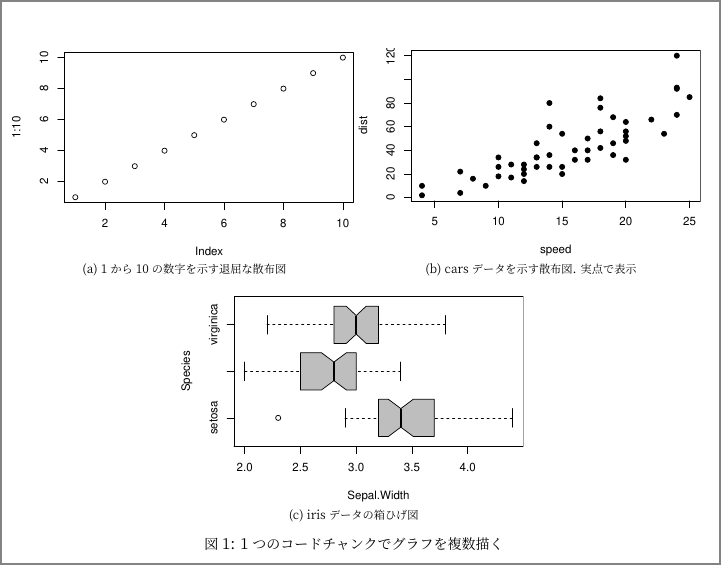
\includegraphics[width=1\linewidth,height=1\textheight,keepaspectratio]{JP/images/latex-subfig} 

}

\caption{複数の図を含む単一の figure 環境の例}\label{fig:latex-subfig}
\end{figure}

\hypertarget{latex-unicode}{%
\section{Unicode 文字を含む文書をレンダリングする}\label{latex-unicode}}

\begin{Shaded}
\begin{Highlighting}[]
\NormalTok{! Package inputenc Error:}
\NormalTok{  Unicode char }\FunctionTok{\textbackslash{}u}\NormalTok{8: not set up for use with LaTeX.}
\end{Highlighting}
\end{Shaded}

もしこのようなエラーにでくわしたら, おそらくデフォルトの LaTeX エンジンである \texttt{pdflatex} を使って文書 (中間ファイルの \texttt{.tex} ) を PDF へレンダリングしているのでしょう. \texttt{pdflatex} はそのファイルにある何らかの Unicode 文字を処理できません. もしこのようなケースであれば, \texttt{xelatex} か \texttt{lualatex} へ切り替える\index{出力オプション!latex\_engine}ことになるでしょう. 例えばこのように.

\begin{Shaded}
\begin{Highlighting}[]
\FunctionTok{output}\KeywordTok{:}
\AttributeTok{  }\FunctionTok{pdf\_document}\KeywordTok{:}
\AttributeTok{    }\FunctionTok{latex\_engine}\KeywordTok{:}\AttributeTok{ xelatex}
\end{Highlighting}
\end{Shaded}

他の文書出力フォーマット, 特に \texttt{bookdown::pdf\_document2} や \texttt{tufte::tufte\_handout} といった \texttt{pdf\_document} ベースのものも LaTeX エンジンも変更できるでしょう. 例えばこのように.

\begin{Shaded}
\begin{Highlighting}[]
\FunctionTok{output}\KeywordTok{:}
\AttributeTok{  bookdown::pdf\_document2}\KeywordTok{:}\FunctionTok{}
\AttributeTok{    }\FunctionTok{latex\_engine}\KeywordTok{:}\AttributeTok{ lualatex}
\AttributeTok{  tufte::tufte\_handout}\KeywordTok{:}\FunctionTok{}
\AttributeTok{    }\FunctionTok{latex\_engine}\KeywordTok{:}\AttributeTok{ xelatex}
\end{Highlighting}
\end{Shaded}

\hypertarget{latex-fragment}{%
\section{LaTeX のコードフラグメントを生成する}\label{latex-fragment}}

もし純粋な LaTeX 文書で作業しているのなら, R Markdown はそれでもやはり便利だと感じているかもしれません. R Markdown で書いて, 文書を他の LaTeX 文書に読み込める LaTeX のコード片 (フラグメント)\index{LaTeX!fragment} に変換したほうが便利なこともあるかもしれません.

Rmd 文書を LaTeX にレンダリングするとき, \texttt{\textbackslash{}documentclass\{\}}, \texttt{\textbackslash{}begin\{body\}}, \texttt{\textbackslash{}end\{body\}} を含む完全な LaTeX 文書が生成されます. フラグメントはこの完全な文書の主に本文の部分です. LaTeX フラグメントをレンダリングするのに, \texttt{latex\_fragment} 出力フォーマットが使えます. 例えばこのように.

\begin{Shaded}
\begin{Highlighting}[]
\PreprocessorTok{{-}{-}{-}}
\FunctionTok{output}\KeywordTok{:}\AttributeTok{ latex\_fragment}
\PreprocessorTok{{-}{-}{-}}
\end{Highlighting}
\end{Shaded}

これは \texttt{.tex} ファイルをレンダリングします. 例えば \texttt{foo.Rmd} は \texttt{foo.tex} にレンダリングされ, 別の LaTeX 文書で \texttt{\textbackslash{}input\{foo.tex\}} を使うことでフラグメントを読み込めます.

\hypertarget{latex-header}{%
\section{カスタムヘッダとフッタ (*)}\label{latex-header}}

LaTeX パッケージの \textbf{fancyhdr}\index{LaTeX パッケージ!fancyhdr} は文書のヘッダとフッタをカスタマイズするいくつかのコマンドを提供します. より完全なガイドとして, \url{https://ctan.org/pkg/fancyhdr} の完全版ドキュメントを参照してください. 最初に, パッケージを読み込みます. それからヘッダのスタイルを変えます. 例えばこのように.

\begin{Shaded}
\begin{Highlighting}[]
\BuiltInTok{\textbackslash{}usepackage}\NormalTok{\{}\ExtensionTok{fancyhdr}\NormalTok{\}}
\FunctionTok{\textbackslash{}pagestyle}\NormalTok{\{fancy\}}
\end{Highlighting}
\end{Shaded}

このパッケージは異なる3つのインターフェースを提示しますが, ここでは \texttt{\textbackslash{}fancyhead} と \texttt{\textbackslash{}fancyfoot} コマンドを使います. 形式を決める構文は \texttt{\textbackslash{}fancyhead{[}selectors{]}\{output\ text\}} で, ここでカスタマイズしたいヘッダの部分がどこかをセレクタが宣言しています. ページの位置を指定する以下のようなセレクタが使えます.

\begin{itemize}
\tightlist
\item
  \textbf{E} 偶数ページ
\item
  \textbf{O} 奇数ページ
\item
  \textbf{L} ページ左側
\item
  \textbf{C} ページ中央
\item
  \textbf{R} ページ右側
\end{itemize}

例えば \texttt{\textbackslash{}fancyhead{[}LE,RO{]}\{あなたの名前\}} は偶数ページの頭の左側と, 奇数ページの頭の右側に「あなたの名前」と印字します. さらに LaTeX コマンドを織り交ぜることで, 各ページの詳細情報を取りだすことができます.

\begin{itemize}
\tightlist
\item
  \texttt{\textbackslash{}thepage}: 現在のページ番号
\item
  \texttt{\textbackslash{}thechapter}: 現在の章番号
\item
  \texttt{\textbackslash{}thesection}: 現在の節番号
\item
  \texttt{\textbackslash{}chaptername}: 英語の ``Chapter'' の単語, あるいは現在の言語でそれに対応するもの, または著者がこのコマンドを再定義してできたテキスト.
\item
  \texttt{\textbackslash{}leftmark}: 大文字で現在のトップレベル構造の名前と番号.
\item
  \texttt{\textbackslash{}rightmark}: 大文字で現在のトップレベル構造に次ぐレベルの名前と番号.
\end{itemize}

以下は LaTeX コードの例で, \ref{latex-preamble}節で紹介した方法でプリアンブルに書き加えることができます.

\begin{Shaded}
\begin{Highlighting}[]
\BuiltInTok{\textbackslash{}usepackage}\NormalTok{\{}\ExtensionTok{fancyhdr}\NormalTok{\}}
\FunctionTok{\textbackslash{}pagestyle}\NormalTok{\{fancy\}}
\CommentTok{\% ヘッダ中央}
\FunctionTok{\textbackslash{}fancyhead}\NormalTok{[CO,CE]\{Your Document Header\}}
\CommentTok{\% フッタ中央}
\FunctionTok{\textbackslash{}fancyfoot}\NormalTok{[CO,CE]\{And this is a fancy footer\}}
\CommentTok{\% 偶数ページ左と奇数ページ右にページ番号}
\FunctionTok{\textbackslash{}fancyfoot}\NormalTok{[LE,RO]\{}\FunctionTok{\textbackslash{}thepage}\NormalTok{\}}
\end{Highlighting}
\end{Shaded}

デフォルトではヘッダとフッタは PDF 文書の最初のページには表示されません. 表示にもフッタを表示したいなら, もう1行 \texttt{\textbackslash{}fancypagestyle\{plain\}\{\textbackslash{}pagestyle\{fancy\}\}} を追加しなければなりません.

\hypertarget{latex-template}{%
\section{Pandoc の LaTeX テンプレートをカスタマイズする (*)}\label{latex-template}}

Pandoc はテンプレート\index{テンプレート!LaTeX} を通じて Markdown を LaTeX に変換します. テンプレートは Pandoc\index{Pandoc} 変数を含む LaTeX ファイルであり, Pandoc はこれらの変数を値に置き換えます. 以下は \texttt{\$body\$} という変数を1つだけ含んだ単純なテンプレートです.

\begin{Shaded}
\begin{Highlighting}[]
\BuiltInTok{\textbackslash{}documentclass}\NormalTok{\{}\ExtensionTok{article}\NormalTok{\}}
\KeywordTok{\textbackslash{}begin}\NormalTok{\{}\ExtensionTok{document}\NormalTok{\}}
\SpecialStringTok{$body$}
\KeywordTok{\textbackslash{}end}\NormalTok{\{}\ExtensionTok{document}\NormalTok{\}}
\end{Highlighting}
\end{Shaded}

\texttt{\$body\$} の値は Markdown ドキュメントの本文から生成された LaTeX コードです. 例えば Markdown で本文が \texttt{Hello **world**!} ならば, \texttt{\$body\$} の値は \texttt{Hello \textbackslash{}textbf\{world\}!} となります.

\ref{latex-preamble}, \ref{latex-variables}, \ref{latex-extra}節で紹介した LaTeX のカスタマイズ方法だけでは不十分なら, 代わりにカスタムテンプレートを使ってみてください. テンプレートはその内部に任意の LaTeX コードを使うことが可能なので, はるかに柔軟です. テンプレートを使うには, \texttt{pdf\_document} の \texttt{template} オプション\index{出力オプション!template} にテンプレートのパスを含めます.

\begin{Shaded}
\begin{Highlighting}[]
\FunctionTok{output}\KeywordTok{:}
\AttributeTok{  }\FunctionTok{pdf\_document}\KeywordTok{:}
\AttributeTok{    }\FunctionTok{template}\KeywordTok{:}\AttributeTok{ my{-}template.tex}
\end{Highlighting}
\end{Shaded}

デフォルトの LaTeX テンプレートは \url{https://github.com/jgm/pandoc/tree/master/data/templates} で見ることができます (ファイル名は \texttt{default.latex}). 自分でテンプレートを作成したい場合, このテンプレートから作りたいと思うことでしょう.

Pandoc 変数の完全なリストとその意味 (\texttt{\$body\$} や \texttt{\$title\$} のような) は Pandoc マニュアルの \url{https://pandoc.org/MANUAL.html\#templates} で見ることができます. 任意のカスタム変数を使うこともでき, それは典型的には YAML メタデータからテンプレートへと与えられます. もし具体例で学びたいなら, \textbf{MonashEBSTemplates} パッケージ\index{R パッケージ!MonashEBSTemplates} (\url{https://github.com/robjhyndman/MonashEBSTemplates}) を確認することもできます. これはいくつかのカスタム LaTeX テンプレートを提供しています. これらのテンプレートは \texttt{inst/rmarkdown/templates/*/resources/} ディレクトリ (\texttt{*} はテンプレート名を指します) 以下にあります. 例えば出力フォーマット \texttt{MonashEBSTemplates::memo} に対するテンプレートは YAML メタデータの変数 \texttt{branding} をモナシュ大学のブランドロゴを含むかどうかをコントロールするのに使えます. このようにテンプレート内で \texttt{if} 文を使うことでこれを実現しています.

\begin{Shaded}
\begin{Highlighting}[]
\SpecialStringTok{$if(branding)$}\CommentTok{\%}
\BuiltInTok{\textbackslash{}includegraphics}\NormalTok{[height=1.5cm]\{}\ExtensionTok{monash2}\NormalTok{\}}
\FunctionTok{\textbackslash{}vspace*}\NormalTok{\{{-}0.6cm\}}
\SpecialStringTok{$else$}
\FunctionTok{\textbackslash{}vspace*}\NormalTok{\{{-}1cm\}}
\SpecialStringTok{$endif$}
\end{Highlighting}
\end{Shaded}

\hypertarget{raw-latex}{%
\section{生の LaTeX コードを書く}\label{raw-latex}}

デフォルトでは Pandoc は LaTeX へ変換する時, 文書内の LaTeX コード\index{LaTeX!生のコード}を維持するので, Markdown 内で LaTeX コマンドや環境を使うことができます. しかし, LaTeX コードが Pandoc がパースするには複雑過ぎるときがあるかもしれず, そのような場合 Pandoc は通常の Markdown として扱います. 結果として特別な LaTeX の文字はエスケープされます. 例えばバックスラッシュ \texttt{\textbackslash{}} は \texttt{\textbackslash{}textbackslash\{\}} に変換されるかもしれません.

Pandoc が Markdown 文書内の生の LaTeX コードに確実に手を付けないようにするには, コードを fenced block で囲み, \texttt{=latex} の属性を付けることもできます. 例えばこのように.

\begin{Shaded}
\begin{Highlighting}[]
\InformationTok{\textasciigrave{}\textasciigrave{}\textasciigrave{}\{=latex\}}
\InformationTok{\textbackslash{}begin\{tabular\}\{ll\}}
\InformationTok{A \& B \textbackslash{}\textbackslash{}}
\InformationTok{A \& B \textbackslash{}\textbackslash{}}
\InformationTok{\textbackslash{}end\{tabular\}}
\InformationTok{\textasciigrave{}\textasciigrave{}\textasciigrave{}}
\end{Highlighting}
\end{Shaded}

\texttt{latex} の前の等号を忘れないでください. つまり \texttt{latex} ではなく \texttt{=latex} です. この機能は Pandoc 2.0 以降のバージョンが必要です (\texttt{rmarkdown::pandoc\_version()} で確認してください).

\hypertarget{latex-hardcore}{%
\section{ハードコア LaTeX ユーザーのために (*)}\label{latex-hardcore}}

R Markdown はきっと執筆と組版のための最善の文書フォーマットではないでしょう. シンプルさは長所であると同時に短所でもあります. LaTeX はタイプすべきコマンドの多さと引き換えに, 組版の観点で Markdown よりはるかに強力です. あなたにとって組版がはるかに優先すべき事項で, あらゆる LaTeX コマンドや環境を使うことに満足しているのなら, 文書全体で Markdown を使う代わりに純粋な LaTeX コードを使うことができます.

\textbf{knitr} パッケージは R Markdown に限定されない多様なソース文書フォーマットをサポートしています. 以下は R コードと純粋な LaTeX コードが混ざり合っている例です

\begin{Shaded}
\begin{Highlighting}[]
\BuiltInTok{\textbackslash{}documentclass}\NormalTok{\{}\ExtensionTok{article}\NormalTok{\}}
\BuiltInTok{\textbackslash{}usepackage}\NormalTok{[T1]\{}\ExtensionTok{fontenc}\NormalTok{\}}

\KeywordTok{\textbackslash{}begin}\NormalTok{\{}\ExtensionTok{document}\NormalTok{\}}

\NormalTok{これがコードチャンクです.}

\NormalTok{\textless{}\textless{}foo, fig.height=4\textgreater{}\textgreater{}=}
\NormalTok{1 + 1}
\NormalTok{par(mar = c(4, 4, .2, .2))}
\NormalTok{plot(rnorm(100))}
\NormalTok{@}

\NormalTok{インライン評価式を書くこともできます. 例えば }\SpecialStringTok{$}\SpecialCharTok{\textbackslash{}pi}\SpecialStringTok{=}\SpecialCharTok{\textbackslash{}Sexpr}\SpecialStringTok{\{pi\}$}\NormalTok{ とか,}
 \FunctionTok{\textbackslash{}Sexpr}\NormalTok{\{1.9910214e28\} で大きな数値を表現できます.}

\KeywordTok{\textbackslash{}end}\NormalTok{\{}\ExtensionTok{document}\NormalTok{\}}
\end{Highlighting}
\end{Shaded}

例えば上記のファイルは \texttt{latex.Rnw} であるようにファイル名はたいてい \texttt{.Rnw}\index{LaTeX!Rnw} という拡張子がつきます. 考え方は同じですが R コードチャンクとインライン R コードを書くための構文が異なっています. R コードチャンクは \texttt{\textless{}\textless{}\textgreater{}\textgreater{}=} で始まり (チャンクオプションは括弧内に書きます), \texttt{@} で終わります. インライン R コードは \texttt{Sexpr\{\}} 内に書きます.

\texttt{knitr::knit()} 関数は \texttt{Rnw} 文書を出力ファイルである LaTeX (\texttt{.tex}) にコンパイルでき, それをさらに \texttt{pdflatex} といった LaTeX ツールを通して PDF にコンパイルできます. \texttt{.Rnw} から PDF を一足でコンパイルするのに \texttt{knitr::knit2pdf()}\index{knitr!knit2pdf()} を使うこともできます. RStudio を使っているならツールバーの \texttt{Compile PDF} を押すこともできます. Rnw 文書をコンパイルする方法のデフォルトは Sweave であり, たぶんあなたは \textbf{knitr} に変更したいだろうということに注意してください (その方法はこの投稿 \url{http://stackoverflow.com/q/27592837/559676} を確認してください).

\texttt{Rnw} 文書は LaTeX のフルパワーをあなたにもたらします. Markdown ではほんとうに解決の難しい組版の問題があるのなら, これは最終手段となるでしょう. ただし, Markdown をやめる前に, カスタム Pandoc LaTeX テンプレート (\ref{latex-template}節参照) もまた役に立つかもしれない, ということも覚えておいてほしいです.

\hypertarget{html-output}{%
\chapter{HTML 出力}\label{html-output}}

LaTeX と比べて HTML はおそらくページに分けた出力の組版が苦手です. しかし, 特に CSS や JavaScript と連携すれば, 結果を見せつける際にははるかに強力になります. 例えば HTML にインタラクティブアプリケーションを埋め込んだり, 動的に HTML ページの外観や, 内容すら修正できます. HTML 出力における有用ながらもシンプルな CSS と JavaScript のトリックは LaTeX 出力で再現するのがとても難しいこともあります (しばしば不可能なこともあります).

この章では, カスタム CSS の適用方法, カスタム HTML テンプレートの使い方, コードブロックのスタイル変更や折りたたみ, 表の内容の並び替え, そして HTML ページへのファイル埋め込みといった, R Markdown の HTML 出力を向上するテクニックを紹介します. In this chapter, we introduce techniques to enhance your HTML output from R Markdown, including how to apply custom CSS rules, use custom HTML templates, style or fold code blocks, arrange content in tabs, and embed files on HTML pages.

\hypertarget{html-css}{%
\section{カスタム CSS を適用する}\label{html-css}}

HTML 文書の外観をカスタマイズしようと思うのなら, CSS と JavaScript を少しでも勉強することを強く勧めます. \textbf{blogdown} 本 \autocite{blogdown2017} の \href{https://bookdown.org/yihui/blogdown/website-basics.html}{Appendix B} には HTML, CSS, JavaScript の簡単なチュートリアルがあります.

CSS のセレクタと優先度のルールを理解することは初心者にとっては極めて重要です. さもなければ自分のカスタム CSS\index{CSS} が意図したように機能しないことに混乱することになるでしょう (おそらく優先度が十分でないから).

Rmd 文書に1つかそれ以上のカスタムスタイルシートを読み込ませるには, \texttt{css} オプション\index{出力オプション!css} を使うことができます. 例えばこのように.

\begin{Shaded}
\begin{Highlighting}[]
\FunctionTok{output}\KeywordTok{:}
\AttributeTok{  }\FunctionTok{html\_document}\KeywordTok{:}
\AttributeTok{    }\FunctionTok{css}\KeywordTok{:}\AttributeTok{ }\StringTok{"style.css"}
\end{Highlighting}
\end{Shaded}

複数のスタイルシートを読み込ませるには, このようにブラケットで囲んだリストを使うことになるでしょう.

\begin{Shaded}
\begin{Highlighting}[]
\FunctionTok{output}\KeywordTok{:}
\AttributeTok{  }\FunctionTok{html\_document}\KeywordTok{:}
\AttributeTok{    }\FunctionTok{css}\KeywordTok{:}\AttributeTok{ }\KeywordTok{[}\StringTok{"style{-}1.css"}\KeywordTok{,}\AttributeTok{ }\StringTok{"style{-}2.css"}\KeywordTok{]}
\end{Highlighting}
\end{Shaded}

あるいは, Rmd 文書に 直接 CSS のルールを埋め込むのに, \texttt{css} コードチャンク\index{言語エンジン!css} を使うこともできます. 例えばこのように.

\begin{Shaded}
\begin{Highlighting}[]
\NormalTok{We embed a }\InformationTok{\textasciigrave{}css\textasciigrave{}}\NormalTok{ code chunk here.}

\InformationTok{\textasciigrave{}\textasciigrave{}\textasciigrave{}\{css, echo=FALSE\}}
\InformationTok{p \{}
\InformationTok{  font{-}size: 32px;}
\InformationTok{\}}
\InformationTok{\textasciigrave{}\textasciigrave{}\textasciigrave{}}
\end{Highlighting}
\end{Shaded}

チャンクオプション \texttt{echo = FALSE}\index{チャンクオプション!echo} は CSS コードを出力にそのまま表示させないことを意味しますが, CSS コードを含む \texttt{\textless{}style\textgreater{}} タグは HTML 出力ファイルにも生成されます.

\hypertarget{center-heading}{%
\section{セクションヘッダを中央揃えにする}\label{center-heading}}

\ref{html-css}節で言及した応用方法のように, CSS を見出しのアラインメント調整\index{CSS プロパティ!text-align}に使うことができます. 例えば以下のような CSS コードを使ってレベル1から3の見出しを中央揃えにしたいかもしれません.

\begin{Shaded}
\begin{Highlighting}[]
\NormalTok{h1}\OperatorTok{,}\NormalTok{ h2}\OperatorTok{,}\NormalTok{ h3 \{}
  \KeywordTok{text{-}align}\NormalTok{: }\DecValTok{center}\OperatorTok{;}
\NormalTok{\}}
\end{Highlighting}
\end{Shaded}

Rmd 文書に CSS を適用する方法は\ref{html-css}節を見てください.

\hypertarget{chunk-styling}{%
\section{コードチャンクのスタイルを変更する}\label{chunk-styling}}

チャンクオプションの \texttt{class.source}\index{チャンクオプション!class.source} と \texttt{class.output}\index{チャンクオプション!class.output} を使い, それぞれコードチャンクおよびそのテキスト出力のスタイルをカスタマイズできます. これらのオプションはクラス名\index{クラス!カスタムクラス}の文字列ベクトルを取ります (\ref{attr-output}節参照). 例えば \texttt{class.source = "important"} は出力時にコードチャンクを含む HTML 要素に \texttt{important} というクラス名を持たせます. そこでこのクラスに CSS ルールを定義できます.\footnote{CSS ではクラスは先頭にピリオド (\texttt{.}) を付けるため, この場合はルールは \texttt{.important} から始まります.} このルールは特定のコードチャンクやテキスト出力を強調したいときに役に立ちます.

デフォルトでは, R Markdown の HTML 出力は Bootstrap フレームワーク\index{Bootstrap}を読み込みます. Bootstrap は \texttt{"bg-primary"}, \texttt{"bg-success"}, \texttt{"bg-info"}, \texttt{"bg-warning"}, \texttt{"bg-danger"} \index{クラス!Bootstrap クラス}\index{クラス!bg-primary}\index{クラス!bg-success}\index{クラス!bg-info}\index{クラス!bg-warning}\index{クラス!bg-danger}といったいくつかの \href{https://getbootstrap.com/docs/3.4/css/\#helper-classes}{背景に対する CSS クラス} が定義済みのため, コードと出力の外観の変更を容易にしてくれます.

以下はチャンクオプション \texttt{class.source = "bg-danger"} と \texttt{class.output = "bg-warning"} を使った例で, その出力は図\ref{fig:chunk-bg}で見られます.

\begin{Shaded}
\begin{Highlighting}[]
\CommentTok{{-}{-}{-}}
\AnnotationTok{title:}\CommentTok{ チャンクのスタイルを変更する}
\AnnotationTok{output:}\CommentTok{ html\_document}
\CommentTok{{-}{-}{-}}

\NormalTok{データフレームの一部を取りだすとき, 必ずしもデータフレームが返されるとは限りません. 例えば2つの列を取りだすなら, データフレームを得ますが, 1つの列を取り出そうとするときは, ベクトルを得ます.}

\InformationTok{\textasciigrave{}\textasciigrave{}\textasciigrave{}\{r class.source="bg{-}danger", class.output="bg{-}warning"\}}
\InformationTok{mtcars[1:5, "mpg"]}
\InformationTok{\textasciigrave{}\textasciigrave{}\textasciigrave{}}

\NormalTok{常に確実にデータフレームを得るようにするには, }\InformationTok{\textasciigrave{}drop = FALSE\textasciigrave{}}\NormalTok{ 引数を使わなければなりません. ここで, チャンクオプション }\InformationTok{\textasciigrave{}class.source = "bg{-}success"\textasciigrave{}}\NormalTok{ を使います.}

\InformationTok{\textasciigrave{}\textasciigrave{}\textasciigrave{}\{r df{-}drop{-}ok, class.source="bg{-}success"\}}
\InformationTok{mtcars[1:5, "mpg", drop = FALSE]}
\InformationTok{\textasciigrave{}\textasciigrave{}\textasciigrave{}}
\end{Highlighting}
\end{Shaded}

\begin{figure}

{\centering 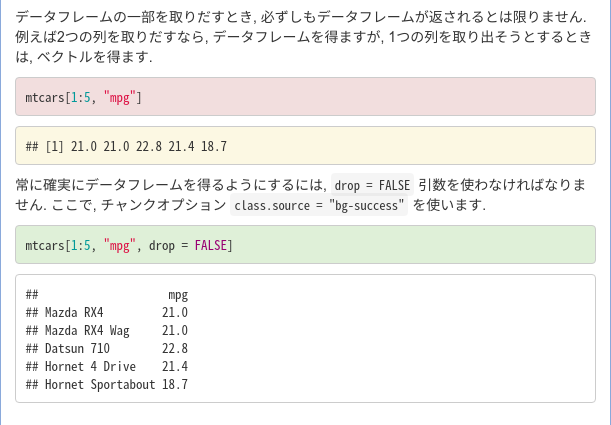
\includegraphics[width=1\linewidth,height=1\textheight,keepaspectratio]{JP/images/chunk-bg} 

}

\caption{Bootstrap で定義された背景色を使ったコードチャンクと出力ブロック}\label{fig:chunk-bg}
\end{figure}

任意のクラスを使って対応する CSS ルールを定義することもできます. この場合, \ref{html-css}節で言及した方法を使ってカスタム CSS ルールを読み込ませなければなりません. 以下はその例です.

\begin{Shaded}
\begin{Highlighting}[]
\CommentTok{{-}{-}{-}}
\AnnotationTok{title:}\CommentTok{ チャンクにカスタムクラスを割り当てる}
\AnnotationTok{output:}\CommentTok{ html\_document}
\CommentTok{{-}{-}{-}}

\NormalTok{まず }\InformationTok{\textasciigrave{}watch{-}out\textasciigrave{}}\NormalTok{ というクラスにいくつか CSSを ルールを定義します.}

\InformationTok{\textasciigrave{}\textasciigrave{}\textasciigrave{}\{css, echo=FALSE\}}
\InformationTok{.watch{-}out \{}
\InformationTok{  background{-}color: lightpink;}
\InformationTok{  border: 3px solid red;}
\InformationTok{  font{-}weight: bold;}
\InformationTok{\}}
\InformationTok{\textasciigrave{}\textasciigrave{}\textasciigrave{}}

\NormalTok{それからチャンクオプション }\InformationTok{\textasciigrave{}class.source\textasciigrave{}}\NormalTok{ で }\InformationTok{\textasciigrave{}watch{-}out\textasciigrave{}}\NormalTok{ クラスをコードチャンクに割り当てます.}

\InformationTok{\textasciigrave{}\textasciigrave{}\textasciigrave{}\{r class.source="watch{-}out"\}}
\InformationTok{mtcars[1:5, "mpg"]}
\InformationTok{\textasciigrave{}\textasciigrave{}\textasciigrave{}}
\end{Highlighting}
\end{Shaded}

図\ref{fig:chunk-border}がスタイルの出力です.

\begin{figure}

{\centering 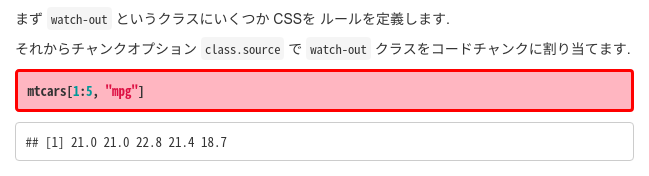
\includegraphics[width=1\linewidth,height=1\textheight,keepaspectratio]{JP/images/chunk-border} 

}

\caption{明桃色の背景, 赤い太枠線をもつコードチャンク}\label{fig:chunk-border}
\end{figure}

文書内の全てのコードブロックにカスタムスタイルを塩要したいなら, グローバルな \textbf{knitr} オプションで \texttt{class.source} を設定します. 例えばこのように.

\begin{Shaded}
\begin{Highlighting}[numbers=left,,]
\NormalTok{knitr}\SpecialCharTok{::}\NormalTok{opts\_chunk}\SpecialCharTok{$}\FunctionTok{set}\NormalTok{(}\AttributeTok{class.source =} \StringTok{"watch{-}out"}\NormalTok{)}
\end{Highlighting}
\end{Shaded}

複数のクラスをコードブロックに適用できます. 例えば \texttt{class.source = c("important", "warning")} でコードブロックに ``important'' と ``warning'' という2つのクラスを持たせられます.

コードブロック全体ではなく, 内部の個別の要素を装飾したいならば, \textbf{flair} パッケージ\index{R パッケージ!flair} \autocite{R-flair} の使用を検討してもよいかもしれません. このパッケージでコードの個別の部分 (特定の文字, 関数名, 引数など) をカスタムスタイル (例えば色, フォントサイズ, あるいはフォントのウエイト) で強調できます.

\hypertarget{html-scroll}{%
\section{コードブロックをスクロール可能にする (*)}\label{html-scroll}}

大量のコードやテキスト出力を HTML ページに表示するとき, 表示範囲の高さを制限したいかもしれません. そうしないとページはとてつもなく長くなり, それらを細かく読む気のない読者に読み飛ばしづらくなるかもしれません. この問題の解決法は複数あります. \texttt{html\_document} フォーマットの \texttt{code\_folding} オプション\index{出力オプション!code\_folding}を使うというのがその1つです. このオプションは出力文書のコードブロックを折りたたみ, また読者はボタンを押して展開することができます (詳細は\ref{fold-show}節).

他の可能性としてはコードブロックが長すぎるとき, 高さを固定しスクロール可能にすることです. これは CSS プロパティの \texttt{max-height}\index{CSS プロパティ!max-height} と \texttt{overflow-y}\index{CSS プロパティ!overflow-y} で実現できます. 以下はその使用例の全容で, 出力は図\ref{fig:html-scroll}になります.

\begin{Shaded}
\begin{Highlighting}[]
\CommentTok{{-}{-}{-}}
\AnnotationTok{title:}\CommentTok{ スクロール可能なコードブロック}
\AnnotationTok{output:}\CommentTok{ html\_document}
\CommentTok{{-}{-}{-}}

\InformationTok{\textasciigrave{}\textasciigrave{}\textasciigrave{}\{css, echo=FALSE\}}
\InformationTok{pre \{}
\InformationTok{  max{-}height: 300px;}
\InformationTok{  overflow{-}y: auto;}
\InformationTok{\}}

\InformationTok{pre[class] \{}
\InformationTok{  max{-}height: 100px;}
\InformationTok{\}}
\InformationTok{\textasciigrave{}\textasciigrave{}\textasciigrave{}}

\NormalTok{コードブロックの高さを制限する CSS ルールをいくつか定義しました. これらのルールがコードブロックとテキスト出力に対して機能するのかテストすることができます.}

\InformationTok{\textasciigrave{}\textasciigrave{}\textasciigrave{}\{r\}}
\InformationTok{\# このチャンクに多くのコードがあるように見せかける}
\InformationTok{if (1 + 1 == 2) \{}
\InformationTok{  \# もちろん真になる}
\InformationTok{  print(mtcars)}
\InformationTok{  \# 単に長いデータを表示させるだけ}
\InformationTok{\}}
\InformationTok{\textasciigrave{}\textasciigrave{}\textasciigrave{}}

\NormalTok{次に高さを100px に制限するために }\InformationTok{\textasciigrave{}scroll{-}100\textasciigrave{}}\NormalTok{ という新しいクラスにルールを追加し,  チャンクオプション }\InformationTok{\textasciigrave{}class.output\textasciigrave{}}\NormalTok{ でこのクラスをコードチャンクの出力に追加します.}

\InformationTok{\textasciigrave{}\textasciigrave{}\textasciigrave{}\{css, echo=FALSE\}}
\InformationTok{.scroll{-}100 \{}
\InformationTok{  max{-}height: 100px;}
\InformationTok{  overflow{-}y: auto;}
\InformationTok{  background{-}color: inherit;}
\InformationTok{\}}
\InformationTok{\textasciigrave{}\textasciigrave{}\textasciigrave{}}

\InformationTok{\textasciigrave{}\textasciigrave{}\textasciigrave{}\{r, class.output="scroll{-}100"\}}
\InformationTok{print(mtcars)}
\InformationTok{\textasciigrave{}\textasciigrave{}\textasciigrave{}}
\end{Highlighting}
\end{Shaded}

\begin{figure}

{\centering 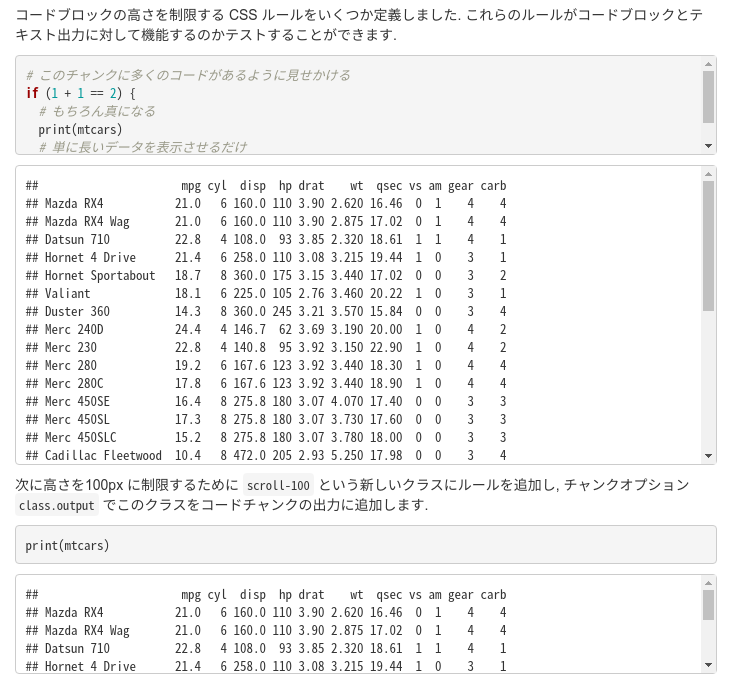
\includegraphics[width=1\linewidth,height=1\textheight,keepaspectratio]{JP/images/html-scroll} 

}

\caption{カスタム CSS を使用したスクロール可能なコードブロック}\label{fig:html-scroll}
\end{figure}

上記の例では全てのコードブロックに大域的に 300px の高さ上限を定義しています. HTML 出力時にはコードブロックが \texttt{\textless{}pre\textgreater{}} タグで囲まれていることを思い出してください. それから \texttt{class} 属性に \texttt{\textless{}pre\textgreater{}} ブロックの高さを 100px に制限します. これは CSS セレクタ \texttt{pre{[}class{]}} が意味するところです. デフォルトではテキスト出力は \texttt{\textless{}pre\textgreater{}\ \textless{}/pre\textgreater{}} に含まれ, R コードブロックは \texttt{\textless{}pre\ class="r"\textgreater{}\ \textless{}/pre\textgreater{}} に含まれます (ここで \texttt{\textless{}pre\textgreater{}} タグが \texttt{class} 属性を持っていることに注意してください).

第2の R コードチャンクからのテキスト出力の高さも 100px です. これが出力にたいして, カスタムクラス名 \texttt{scroll-100} を割り当て, 高さの上限を 100px に定義した理由です.

個別のコードブロックに対して異なる最大高さを指定したいならば, \ref{hook-scroll}節の例を見ることもできます.

\hypertarget{fold-show}{%
\section{全コードブロックを折りたたみ, かついくつかは表示する}\label{fold-show}}

出力文書に書かれたコードブロックが読者に嫌がられるおそれがあるなら, はじめは折りたたんでおくという選択をするとよいかもしれません. 読者はボタンを押して表示を選ぶことができます.

\begin{Shaded}
\begin{Highlighting}[]
\FunctionTok{output}\KeywordTok{:}
\AttributeTok{  }\FunctionTok{html\_document}\KeywordTok{:}
\AttributeTok{    }\FunctionTok{code\_folding}\KeywordTok{:}\AttributeTok{ hide}
\end{Highlighting}
\end{Shaded}

全てのコードブロックを最初から展開することもできます (よって読者は折りたたむことを選べます).

\begin{Shaded}
\begin{Highlighting}[]
\FunctionTok{output}\KeywordTok{:}
\AttributeTok{  }\FunctionTok{html\_document}\KeywordTok{:}
\AttributeTok{    }\FunctionTok{code\_folding}\KeywordTok{:}\AttributeTok{ show}
\end{Highlighting}
\end{Shaded}

最初から全てのコードブロックを折りたたんだなら, チャンクオプション \texttt{class.source = "fold-show"} を使い特定のブロックを展開だけを最初から展開させておくこともできます. このように.

\begin{Shaded}
\begin{Highlighting}[]
\CommentTok{{-}{-}{-}}
\AnnotationTok{title:}\CommentTok{ Hide all code blocks and show some initially}
\AnnotationTok{output:}
\CommentTok{  html\_document:}
\CommentTok{    code\_folding: hide}
\CommentTok{{-}{-}{-}}

\InformationTok{\textasciigrave{}\textasciigrave{}\textasciigrave{}\{r\}}
\InformationTok{1  \# code is hidden initially}
\InformationTok{\textasciigrave{}\textasciigrave{}\textasciigrave{}}

\InformationTok{\textasciigrave{}\textasciigrave{}\textasciigrave{}\{r class.source = \textquotesingle{}fold{-}show\textquotesingle{}\}}
\InformationTok{2  \# code is shown initially}
\InformationTok{\textasciigrave{}\textasciigrave{}\textasciigrave{}}

\InformationTok{\textasciigrave{}\textasciigrave{}\textasciigrave{}\{r\}}
\InformationTok{3  \# also hidden}
\InformationTok{\textasciigrave{}\textasciigrave{}\textasciigrave{}}
\end{Highlighting}
\end{Shaded}

反対のこともできます. つまり, 最初から全てのコードブロックを表示するもののそれらの一部は表示させます. 例えばこのように.

\begin{Shaded}
\begin{Highlighting}[]
\CommentTok{{-}{-}{-}}
\AnnotationTok{output:}
\CommentTok{  html\_document:}
\CommentTok{    code\_folding: show}
\CommentTok{{-}{-}{-}}

\InformationTok{\textasciigrave{}\textasciigrave{}\textasciigrave{}\{r\}}
\InformationTok{1  \# code is shown initially}
\InformationTok{\textasciigrave{}\textasciigrave{}\textasciigrave{}}

\InformationTok{\textasciigrave{}\textasciigrave{}\textasciigrave{}\{r class.source = \textquotesingle{}fold{-}hide\textquotesingle{}\}}
\InformationTok{2  \# code is hidden initially}
\InformationTok{\textasciigrave{}\textasciigrave{}\textasciigrave{}}
\end{Highlighting}
\end{Shaded}

\hypertarget{html-tabs}{%
\section{内容をタブブラウジングさせる}\label{html-tabs}}

HTML レポートの並列しているセクションをまとめる自然な方法の1つは, タブセットを使うことです. これは読者がページをスクロールして戻したり進めたりするかわりに, タブのタイトルをクリックすることで異なるセクションの内容を閲覧することを可能にします.

セクションをタブにするために, タブに変換する見出しより1レベル上の見出しにクラス属性 \texttt{.tabset}\index{tabset} を追加できます. 例えばレベル2の見出しに \texttt{.tabset} を追加するとそれ以降のレベル3の見出しが全てタブに変換されます. 以下は用例の全容です.

\begin{Shaded}
\begin{Highlighting}[]
\CommentTok{{-}{-}{-}}
\AnnotationTok{title:}\CommentTok{ 内容をタブにまとめる}
\AnnotationTok{output:}\CommentTok{ html\_document}
\CommentTok{{-}{-}{-}}

\InformationTok{\textasciigrave{}html\_document\textasciigrave{}}\NormalTok{ 出力で並列するセクションをタブにできます.}

\FunctionTok{\#\# 結果 \{.tabset\}}

\FunctionTok{\#\#\# グラフ}

\NormalTok{このセクションでは散布図を表示します.}

\InformationTok{\textasciigrave{}\textasciigrave{}\textasciigrave{}\{r, fig.dim=c(5, 3)\}}
\InformationTok{par(mar = c(4, 4, .5, .1))}
\InformationTok{plot(mpg \textasciitilde{} hp, data = mtcars, pch = 19)}
\InformationTok{\textasciigrave{}\textasciigrave{}\textasciigrave{}}

\FunctionTok{\#\#\# 表}

\NormalTok{このタブではデータを表示します.}

\InformationTok{\textasciigrave{}\textasciigrave{}\textasciigrave{}\{r\}}
\InformationTok{head(mtcars)}
\InformationTok{\textasciigrave{}\textasciigrave{}\textasciigrave{}}
\end{Highlighting}
\end{Shaded}

出力を図\ref{fig:html-tabs}に示します. 実際には一度に1つのタブしか見られないことに注意してください. この図は両方のタブがみられるよう2つのスクリーンショットを連結したものです.

\begin{figure}

{\centering 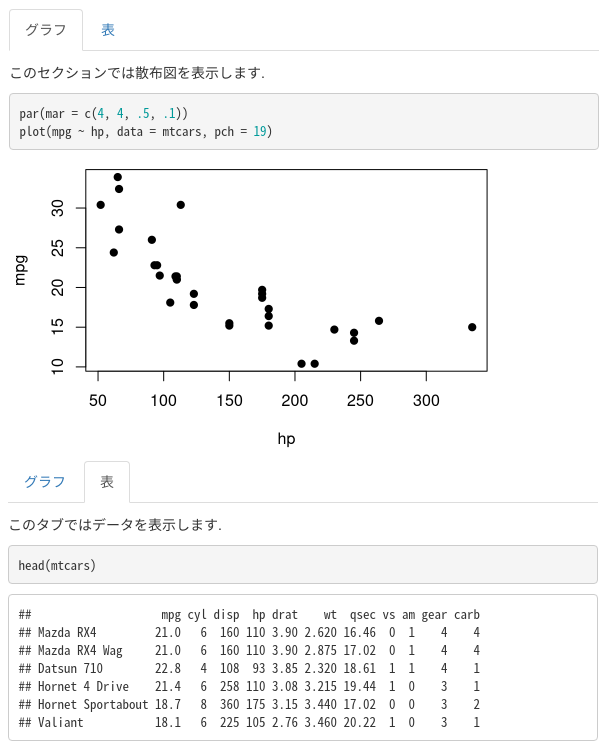
\includegraphics[width=1\linewidth,height=1\textheight,keepaspectratio]{JP/images/html-tabs} 

}

\caption{複数のセクションをタブに}\label{fig:html-tabs}
\end{figure}

タブに ``pill'' 効果を付けるため, さらに別の属性 \texttt{.tabset-pills} を上位レベルの見出しに追加することができます. これでタブは暗青色の背景になります.

\begin{Shaded}
\begin{Highlighting}[]
\FunctionTok{\#\# Results \{.tabset .tabset{-}pills\}}
\end{Highlighting}
\end{Shaded}

デフォルトでは最初のタブがアクティブ (つまり表示されている) です. 他のタブを最初に表示させたいなら, そのセクションに \texttt{.active} 属性を追加することもできます.

タブセットを終わらせるには, 上位レベルのセクション見出しを新しく開始する必要があります. 新しいセクションの見出しは空にすることができます. 例えばこのように.

\begin{Shaded}
\begin{Highlighting}[]
\FunctionTok{\#\# Results \{.tabset\}}

\FunctionTok{\#\#\# Tab One}

\FunctionTok{\#\#\# Tab Two}

\FunctionTok{\#\# \{{-}\}}

\NormalTok{上記のように番号なし (}\InformationTok{\textasciigrave{}\{{-}\}\textasciigrave{}}\NormalTok{) で空のセクション見出しがあれば,}
\NormalTok{タブセットを終了しさらなる段落を続けることができます.}
\end{Highlighting}
\end{Shaded}

\hypertarget{embed-rmd}{%
\section{Rmd ソースファイルを HTML に埋め込む}\label{embed-rmd}}

HTML 出力ページを共有するとき, Rmd ソースファイルもほしいかもしれません. 例えば Rmd ソースを変更し, 自分自身でレポートをコンパイルしたいかもしれません. Rmd ソースファイルのコピーを HTML に埋め込むにはオプション \texttt{code\_download}\index{出力オプション!code\_download} を使うことができます.

\begin{Shaded}
\begin{Highlighting}[]
\FunctionTok{output}\KeywordTok{:}
\AttributeTok{  }\FunctionTok{html\_document}\KeywordTok{:}
\AttributeTok{    }\FunctionTok{code\_download}\KeywordTok{:}\AttributeTok{ }\CharTok{true}
\end{Highlighting}
\end{Shaded}

オプションが有効になると, HTML 出力ページはダウンロードボタンを持ち, 読者はそのボタンを押してソースファイルのダウンロードができます.

\hypertarget{embed-file}{%
\section{HTML 出力に好きなファイルを埋め込む}\label{embed-file}}

\ref{embed-rmd}節で言及したように, HTML出力には Rmd ソース文書のコピーを埋め込めます. Rmd ファイル単体ではレポートを再現するのに不十分な場合もあるかもしれません. 例えばレポートに外部のデータファイルが必要かもしれません. HTML 出力ファイルに好きなファイルを埋め込んでくれる一連の関数が \textbf{xfun} パッケージ\index{R パッケージ!xfun} \autocite{R-xfun} にあります. これらの関数を使うために, 以下の R パッケージを用意しておきます.

\begin{Shaded}
\begin{Highlighting}[numbers=left,,]
\NormalTok{xfun}\SpecialCharTok{::}\FunctionTok{pkg\_load2}\NormalTok{(}\FunctionTok{c}\NormalTok{(}\StringTok{"htmltools"}\NormalTok{, }\StringTok{"mime"}\NormalTok{))}
\end{Highlighting}
\end{Shaded}

これで1つ以上のファイルやディレクトリを HTML 出力に埋め込むのに, コードチャンク内で \texttt{xfun::embed\_file()}\index{xfun!embed\_file()}, \texttt{xfun::embed\_files()}\index{xfun!embed\_files()}, \texttt{xfun::embed\_dir()}\index{xfun!embed\_dir()} を使えます. 例えばこのように.

\begin{Shaded}
\begin{Highlighting}[]
\InformationTok{\textasciigrave{}\textasciigrave{}\textasciigrave{}\{r echo=FALSE\}}
\InformationTok{\# a single file}
\InformationTok{xfun::embed\_file(\textquotesingle{}source.Rmd\textquotesingle{})}

\InformationTok{\# multiple files}
\InformationTok{xfun::embed\_files(c(\textquotesingle{}source.Rmd\textquotesingle{}, \textquotesingle{}data.csv\textquotesingle{}))}

\InformationTok{\# a directory}
\InformationTok{xfun::embed\_dir(\textquotesingle{}data/\textquotesingle{}, text = \textquotesingle{}Download full data\textquotesingle{})}
\InformationTok{\textasciigrave{}\textasciigrave{}\textasciigrave{}}
\end{Highlighting}
\end{Shaded}

プログラミング的にファイルのリストを与えることもできます. 例えばこのように.

\begin{Shaded}
\begin{Highlighting}[numbers=left,,]
\CommentTok{\# embed all Rmd and csv files}
\NormalTok{xfun}\SpecialCharTok{::}\FunctionTok{embed\_files}\NormalTok{(}\FunctionTok{list.files}\NormalTok{(}\StringTok{"."}\NormalTok{, }\StringTok{"[.](Rmd|csv)$"}\NormalTok{))}
\end{Highlighting}
\end{Shaded}

複数のファイルに対し, これらの関数はまず zip ファイルに圧縮してから, この zip ファイルを埋め込みます. これらの関数はリンクを返し, 読者は HTML ページのリンクをクリックして埋め込んだファイルをダウンロードすることができます.

ヘルプページ \texttt{?xfun::embed\_file} またはブログ投稿 \url{https://yihui.org/en/2018/07/embed-file/} でこれらの関数のより詳細な技術的情報を学ぶことができます. 同様のアイディアにより, \textbf{downloadthis} package\index{R パッケージ!downloadthis} \autocite{R-downloadthis} はダウンロードボタンを実装したことでユーザーはリンクではなくダウンロードボタンをクリックしてダウンロードできるようになります. ボタンを使うほうがお好みなら, こちらを使うことも検討するとよいでしょう.

\hypertarget{html-template}{%
\section{カスタム HTML テンプレートを使う (*)}\label{html-template}}

既に\ref{latex-template}節では LaTeX テンプレートについて話しました. Pandoc が Markdown を HTML へ変換するに際しカスタム HTML テンプレート \index{テンプレート!HTML}を指定することもできます. 以下は簡単なテンプレートの例です.

\begin{Shaded}
\begin{Highlighting}[]
\KeywordTok{\textless{}html\textgreater{}}
  \KeywordTok{\textless{}head\textgreater{}}
    \KeywordTok{\textless{}title\textgreater{}}\NormalTok{$title$}\KeywordTok{\textless{}/title\textgreater{}}
\NormalTok{    $for(css)$}
    \KeywordTok{\textless{}link}\OtherTok{ rel=}\StringTok{"stylesheet"}\OtherTok{ href=}\StringTok{"$css$"}\OtherTok{ type=}\StringTok{"text/css"} \KeywordTok{/\textgreater{}}
\NormalTok{    $endfor$}
  \KeywordTok{\textless{}/head\textgreater{}}
  \KeywordTok{\textless{}body\textgreater{}}
\NormalTok{  $body$}
  \KeywordTok{\textless{}/body\textgreater{}}
\KeywordTok{\textless{}/html\textgreater{}}
\end{Highlighting}
\end{Shaded}

テンプレートに \texttt{\$title\$}, \texttt{\$body\$} といったいくつかの変数が含まれているのがわかるでしょう. Pandoc 変数の完全なリストとそれぞれの意味については \url{https://pandoc.org/MANUAL.html\#templates} で検索することができます.

テンプレートによってあなたは HTML 出力をカスタマイズする究極の力を得ることになります. 例えば好きな CSS スタイルシートや JavaScript コード, あるいはライブラリを \texttt{\textless{}head\textgreater{}} 内で読み込ませたりできます. あるいは文書が下書きか, 最終稿かを示すブーリアン変数 \texttt{draft} も使えます.

\begin{Shaded}
\begin{Highlighting}[]
\KeywordTok{\textless{}head\textgreater{}}
\KeywordTok{\textless{}style}\OtherTok{ type=}\StringTok{"text/css"}\KeywordTok{\textgreater{}}
\FunctionTok{.logo}\NormalTok{ \{}
  \KeywordTok{float}\NormalTok{: }\DecValTok{right}\OperatorTok{;}
\NormalTok{\}}
\KeywordTok{\textless{}/style\textgreater{}}
\KeywordTok{\textless{}/head\textgreater{}}

\KeywordTok{\textless{}body\textgreater{}}
\KeywordTok{\textless{}div}\OtherTok{ class=}\StringTok{"logo"}\KeywordTok{\textgreater{}}
\NormalTok{$if(draft)$}
\CommentTok{\textless{}!{-}{-} use draft.png to show that this is a draft {-}{-}\textgreater{}}
\KeywordTok{\textless{}img}\OtherTok{ src=}\StringTok{"images/draft.png"}\OtherTok{ alt=}\StringTok{"Draft mode"} \KeywordTok{/\textgreater{}}
\NormalTok{$else$}
\CommentTok{\textless{}!{-}{-} insert the formal logo if this is final {-}{-}\textgreater{}}
\KeywordTok{\textless{}img}\OtherTok{ src=}\StringTok{"images/logo.png"}\OtherTok{ alt=}\StringTok{"Final version"} \KeywordTok{/\textgreater{}}
\NormalTok{$endif$}
\KeywordTok{\textless{}/div\textgreater{}}

\NormalTok{$body$}
\KeywordTok{\textless{}/body\textgreater{}}
\end{Highlighting}
\end{Shaded}

すると Rmd 文書の YAML メタデータ内で \texttt{draft} 変数に \texttt{true} または \texttt{false} を設定できます. 例えばこのように.

\begin{Shaded}
\begin{Highlighting}[]
\PreprocessorTok{{-}{-}{-}}
\FunctionTok{title}\KeywordTok{:}\AttributeTok{ }\StringTok{"An Important Report"}
\FunctionTok{draft}\KeywordTok{:}\AttributeTok{ }\CharTok{true}
\PreprocessorTok{{-}{-}{-}}
\end{Highlighting}
\end{Shaded}

テンプレートを Rmd 文書に適用するのに, テンプレートをファイルに保存し, \texttt{html\_document} の \texttt{template} オプション\index{出力オプション!template}にファイルパスを与えることができます. 例えばこのように.

\begin{Shaded}
\begin{Highlighting}[]
\FunctionTok{output}\KeywordTok{:}
\AttributeTok{  }\FunctionTok{html\_document}\KeywordTok{:}
\AttributeTok{    }\FunctionTok{template}\KeywordTok{:}\AttributeTok{ my{-}template.html}
\end{Highlighting}
\end{Shaded}

\textbf{rmarkdown} パッケージは Pandoc のデフォルトテンプレートとは異なるカスタム HTML テンプレートをパッケージ内で読み込んで使用しています. Pandoc のデフォルトを使うには \texttt{template: null} で指定できます.

\hypertarget{include-html}{%
\section{既存の HTML ファイルの内容を読み込む (*)}\label{include-html}}

\texttt{html\_document} フォーマット (あるいはこのオプションをサポートしている他のフォーマット) の \texttt{includes} オプション\index{出力オプション!includes} があれば, 既存の HTML ファイルの本文を HTML 出力文書の3箇所のどこかで読み込むことができます. それらは \texttt{\textless{}head\textgreater{}}, \texttt{\textless{}body\textgreater{}} の開始時点, そして \texttt{\textless{}/body\textgreater{}} の末尾です.

\begin{Shaded}
\begin{Highlighting}[]
\FunctionTok{output}\KeywordTok{:}
\AttributeTok{  }\FunctionTok{html\_document}\KeywordTok{:}
\AttributeTok{    }\FunctionTok{includes}\KeywordTok{:}
\AttributeTok{      }\FunctionTok{in\_header}\KeywordTok{:}\AttributeTok{ header.html}
\AttributeTok{      }\FunctionTok{before\_body}\KeywordTok{:}\AttributeTok{ before.html}
\AttributeTok{      }\FunctionTok{after\_body}\KeywordTok{:}\AttributeTok{ after.html}
\end{Highlighting}
\end{Shaded}

HTML にあまり詳しくないなら, \ref{html-template}節がこのオプションをより理解するのに役に立つかもしれません.

\texttt{in\_header} オプションを使うなら, CSS と JavaScript コードを \texttt{\textless{}head\textgreater{}} タグ内に挿入することができます. \texttt{before\_body} を使うなら, バナーやロゴを表示するヘッダを埋め込むこともできます. \texttt{after\_body} を使うなら, フッタを読み込ませることができます. 例えばこのように.

\begin{Shaded}
\begin{Highlighting}[]
\KeywordTok{\textless{}div}\OtherTok{ class=}\StringTok{"footer"}\KeywordTok{\textgreater{}}\NormalTok{Copyright }\DecValTok{\&copy;}\NormalTok{ John Doe 2020}\KeywordTok{\textless{}/div\textgreater{}}
\end{Highlighting}
\end{Shaded}

外部 HTML ファイルの内容を本文の好きな位置で読み込みたいときもあるかもしれません. これは \texttt{htmltools::includeHTML()} を使えば可能です. HTML ファイルパスをこの関数に与えます. 関数はこのファイルを読み込み, 出力文書にたいしてこのファイルの中身を書き込みます. \ref{raw-content}節で使用したようなテクニックをを使っても良いかもしれません. 例えばこのように.

\begin{Shaded}
\begin{Highlighting}[]
\InformationTok{\textasciigrave{}\textasciigrave{}\textasciigrave{}\textasciigrave{}\{=html\}}
\InformationTok{\textasciigrave{}\textasciigrave{}\textasciigrave{}\{r, echo=FALSE, results=\textquotesingle{}asis\textquotesingle{}\}}
\InformationTok{xfun::file\_string(\textquotesingle{}file.html\textquotesingle{})}
\InformationTok{\textasciigrave{}\textasciigrave{}\textasciigrave{}}
\InformationTok{\textasciigrave{}\textasciigrave{}\textasciigrave{}\textasciigrave{}}
\end{Highlighting}
\end{Shaded}

HTML ファイル内読み込めるのは別の HTML 部分だけであり, 完全なHTMLファイルを読み込んではならないことに注意してください. 完全な HTML ファイルとは \texttt{\textless{}html\textgreater{}} タグを含むものであり, これは他の \texttt{\textless{}html\textgreater{}} タグ内に埋め込むことができません. 以下は HTML 文書に別の完全な HTML 文書が 埋め込まれた場合の無効な HTML 文書です.

\begin{Shaded}
\begin{Highlighting}[]
\KeywordTok{\textless{}html\textgreater{}}
  \KeywordTok{\textless{}head\textgreater{}}  \KeywordTok{\textless{}/head\textgreater{}}

  \KeywordTok{\textless{}body\textgreater{}}
\NormalTok{  親 HTML ファイル.}

  \CommentTok{\textless{}!{-}{-} 以下 htmltools::includeHTML() {-}{-}\textgreater{}}
    \KeywordTok{\textless{}html\textgreater{}}
      \KeywordTok{\textless{}head\textgreater{}}  \KeywordTok{\textless{}/head\textgreater{}}
      \KeywordTok{\textless{}body\textgreater{}}
\NormalTok{      子 HTML ファイル.}
      \KeywordTok{\textless{}/body\textgreater{}}
    \KeywordTok{\textless{}/html\textgreater{}}
  \CommentTok{\textless{}!{-}{-} 読み込み終わり {-}{-}\textgreater{}}

  \KeywordTok{\textless{}/body\textgreater{}}
\KeywordTok{\textless{}/html\textgreater{}}
\end{Highlighting}
\end{Shaded}

HTML ファイルを別の HTML 出力文書に読み込む時に問題が発生したなら, HTML ファイルに \texttt{\textless{}html\textgreater{}} タグが含まれていないか確認するとよいかもしれません.

\textbf{rmarkdown} パッケージには \texttt{html\_fragment} という出力フォーマットがあり, 完全な HTML 文書の代わりに HTML の一部を生成します. Rmd 文書内で別のコンパイルされた Rmd 文書の結果を読み込みたい場合, 後者の Rmd 文書は \texttt{html\_document} フォーマットの代わりに \texttt{html\_fragment} フォーマットを使うこともできます.

HTML ファイルの代わりに Rmd または Markdown 文書を読み込ませたいなら, \ref{child-document}節で紹介されている子文書を使うこともできます.

\hypertarget{favicon}{%
\section{ブラウザアイコンをカスタマイズする}\label{favicon}}

\ref{include-html}節では \texttt{html\_document} フォーマットの \texttt{includes} オプションで追加のコードを HTML のヘッダ, 本文, フッタに挿入できることを実演しました. このテクニックはファビコン\index{図!ファビコン}というカスタムブラウザアイコンを HTML 出力に追加することに使えます.

ファビコンはブラウザのアドレスバー, タブタイトル, ブックマークに表示されるウェブサイトのロゴです. 例えば Google Chrome で CRAN のウェブサイト (\url{https://cran.r-project.org}) を開いてブラウザのタブを見ると, 小さな R ロゴがあります. 携帯端末ならばファビコンはウェブサイトをホームスクリーンに固定表示した際にアプリアイコンの代わりに使われます.

HTML 文書にファビコンを追加するには, 以下のコードをカスタムヘッダファイル (\ref{include-html}節で言及したように, \texttt{header.html} といった名前のファイル) を追加します.

\begin{Shaded}
\begin{Highlighting}[]
\KeywordTok{\textless{}link}\OtherTok{ rel=}\StringTok{"shortcut icon"}\OtherTok{ href=}\StringTok{"\{ファビコン画像ファイルへのパス\}"} \KeywordTok{/\textgreater{}}
\end{Highlighting}
\end{Shaded}

YAML メタデータ\index{出力オプション!includes}を使って, このファイルを文書の \texttt{\textless{}head\textgreater{}} 内に挿入できることを思い出してください.

\begin{Shaded}
\begin{Highlighting}[]
\FunctionTok{output}\KeywordTok{:}
\AttributeTok{  }\FunctionTok{html\_document}\KeywordTok{:}
\AttributeTok{    }\FunctionTok{includes}\KeywordTok{:}
\AttributeTok{      }\FunctionTok{in\_header}\KeywordTok{:}\AttributeTok{ header.html}
\end{Highlighting}
\end{Shaded}

\texttt{\textless{}link\textgreater{}} の \texttt{href} 属性に与えたパスは他のアセット (例えば画像やデータ・セット) を参照するときと同じように, 相対パス構造を前提とすべきです. 使用する画像は, 最も小さい正方形の PNG ファイルがよく機能します. 典型的なウェブブラウザは画像を 16 x 16 ピクセルの領域に表示するため, シンプルなデザインがより良いということに留意してください.

あなたの文書を表示するそれぞれのブラウザやプラットフォームは特定のレイアウトに対して最適な解像度のバージョンを使用します. ファビコンセットとより複雑な HTML ヘッダのコードを生成するのに, \url{https://realfavicongenerator.net} といったサービスを使うとよいかもしれません. このサービスは現在 \textbf{pkgdown} パッケージ \autocite{R-pkgdown} の \texttt{pkgdown::build\_favicon()} 関数で R パッケージロゴのセットを作り出すのに使用されています.

\hypertarget{details-tag}{%
\section{\texorpdfstring{折りたたみ要素 \texttt{\textless{}details\textgreater{}} を使う}{折りたたみ要素 \textless details\textgreater{} を使う}}\label{details-tag}}

\ref{html-scroll}節で言及したように, \texttt{html\_document} フォーマットの \texttt{code\_folding: hide} オプションでソースコードチャンクを折りたたむことができます. 現在は出力ブロックを折りたたむことはできませんが, 出力を折りたたみできるようにするのに JavaScript のトリックが使えます. これは出力が比較的長く, しかしさほど重要でないときに役に立つでしょう. 初期状態で折りたたみ, 読者が興味を持てば内容を見るために展開することができます. 図\ref{fig:details-tag}はその例です. 「詳細」ボタンをクリックして出力を展開できるでしょう.

\begin{figure}

{\centering 
\includegraphics[width=1\linewidth,height=1\textheight,keepaspectratio]{JP/images/details-closed} 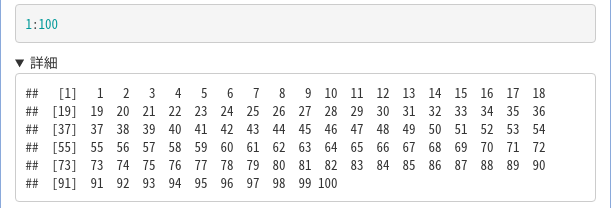
\includegraphics[width=1\linewidth,height=1\textheight,keepaspectratio]{JP/images/details-open} 

}

\caption{details 要素でテキスト出力を囲む}\label{fig:details-tag}
\end{figure}

あなたがご覧になっているのが本書の HTML バージョンなら, 以下のチャンクで実際に動くのを見ることができます. PDF または印刷版を読んでいるのなら, このような対話的機能 (「詳細」ボタンを押すこと) はおそらく不可能です.

\begin{Shaded}
\begin{Highlighting}[numbers=left,,]
\DecValTok{1}\SpecialCharTok{:}\DecValTok{100}
\end{Highlighting}
\end{Shaded}

\begin{verbatim}
##   [1]   1   2   3   4   5   6   7   8   9  10  11  12
##  [13]  13  14  15  16  17  18  19  20  21  22  23  24
##  [25]  25  26  27  28  29  30  31  32  33  34  35  36
##  [37]  37  38  39  40  41  42  43  44  45  46  47  48
##  [49]  49  50  51  52  53  54  55  56  57  58  59  60
##  [61]  61  62  63  64  65  66  67  68  69  70  71  72
##  [73]  73  74  75  76  77  78  79  80  81  82  83  84
##  [85]  85  86  87  88  89  90  91  92  93  94  95  96
##  [97]  97  98  99 100
\end{verbatim}

以下は出力ブロックを検出し, それを \texttt{\textless{}details\textgreater{}} タグで囲む JavaScript コードを読み込ませた Rmd 文書の完全なソースです.

\begin{Shaded}
\begin{Highlighting}[]
\CommentTok{{-}{-}{-}}
\AnnotationTok{title:}\CommentTok{ 折りたたみ要素 \textasciigrave{}\textless{}details\textgreater{}\textasciigrave{} を使う}
\AnnotationTok{output:}\CommentTok{ html\_document}
\CommentTok{{-}{-}{-}}

\NormalTok{この例ではテキスト出力を }\InformationTok{\textasciigrave{}\textless{}details\textgreater{}\textasciigrave{}}\NormalTok{ タグ内に表示します.}
\NormalTok{JavaScript でテキスト出力ブロックを }\InformationTok{\textasciigrave{}\textless{}details\textgreater{}\textless{}/details\textgreater{}\textasciigrave{}}\NormalTok{ で囲みます.}
\NormalTok{Javascript コードはこの文書の末尾で実行する必要があるため,}
\NormalTok{最後に配置します. 以下はテスト用のコードチャンクです.}

\InformationTok{\textasciigrave{}\textasciigrave{}\textasciigrave{}\{r\}}
\InformationTok{1:100}
\InformationTok{\textasciigrave{}\textasciigrave{}\textasciigrave{}}

\NormalTok{実際の JavaScript コードは以下になります.}

\InformationTok{\textasciigrave{}\textasciigrave{}\textasciigrave{}\{js, echo=FALSE\}}
\InformationTok{(function() \{}
\InformationTok{  var codes = document.querySelectorAll(\textquotesingle{}pre:not([class])\textquotesingle{});}
\InformationTok{  var code, i, d, s, p;}
\InformationTok{  for (i = 0; i \textless{} codes.length; i++) \{}
\InformationTok{    code = codes[i];}
\InformationTok{    p = code.parentNode;}
\InformationTok{    d = document.createElement(\textquotesingle{}details\textquotesingle{});}
\InformationTok{    s = document.createElement(\textquotesingle{}summary\textquotesingle{});}
\InformationTok{    s.innerText = \textquotesingle{}詳細\textquotesingle{};}
\InformationTok{    // \textless{}details\textgreater{}\textless{}summary\textgreater{}詳細\textless{}/summary\textgreater{}\textless{}/details\textgreater{}}
\InformationTok{    d.appendChild(s);}
\InformationTok{    // コードを \textless{}details\textgreater{} 内に移動}
\InformationTok{    p.replaceChild(d, code);}
\InformationTok{    d.appendChild(code);}
\InformationTok{  \}}
\InformationTok{\})();}
\InformationTok{\textasciigrave{}\textasciigrave{}\textasciigrave{}}
\end{Highlighting}
\end{Shaded}

上記の JavaScript コードを自分で適用することもできます. ポイントは要素を \texttt{\textless{}details\textgreater{}} で囲むということです.

\begin{Shaded}
\begin{Highlighting}[]
\BuiltInTok{document}\OperatorTok{.}\FunctionTok{querySelectorAll}\NormalTok{(}\StringTok{\textquotesingle{}pre:not([class])\textquotesingle{}}\NormalTok{)}\OperatorTok{;}
\end{Highlighting}
\end{Shaded}

CSS セレクタの \texttt{pre:not({[}class{]})} は \texttt{class} 属性のない全ての \texttt{\textless{}pre\textgreater{}} 要素を意味します. 他の要素のタイプを選択することもできます. CSS セレクタについてより知りたいなら, \url{https://www.w3schools.com/css/css_selectors.asp} を見てください. HTML タグ \texttt{\textless{}details\textgreater{}} と \texttt{\textless{}summary\textgreater{}} をより知りたいなら, \url{https://www.w3schools.com/tags/tag_details.asp} を見てください.

\hypertarget{html-share}{%
\section{HTML 出力を Web で共有する}\label{html-share}}

R Markdown を HTML ファイルにレンダリングするということの魅力的な側面の1つは, これらのファイルをとても簡単にインターネットでホストし他のウェブサイトと同様に共有できるということです. この節では貴方の作成した HTML\index{HTML ホスティング} 文書を共有するオプションを簡単に要約します.

\hypertarget{r-specific-services}{%
\subsection{R 特化のサービス}\label{r-specific-services}}

RStudio は R Markdown で作られた様々な種類のコンテンツをインターネットで公開するためのサービスをいくつか提案しています. これらのサービスは特に RStudio IDE または \textbf{rsconnect} パッケージ \autocite{R-rsconnect} を使って簡単に公開できます.

\begin{itemize}
\item
  \href{https://rpubs.com}{\textbf{RPubs}} は静的な単一の R Markdown コンテンツの無料ホスティングを可能とします. RStudio IDE の \texttt{Publish} ボタンまたは \texttt{rsconnect::rpubsUpload()} 関数で簡単に公開できます. 詳細は ``Getting Started'' のページ (\url{https://rpubs.com/about/getting-started}) をご覧ください.
\item
  \href{https://www.shinyapps.io}{\textbf{ShinyApps.io}} は R を実行するサーバを要求するような動的コンテンツのホスティングを可能にします. 例えば Shiny コンポネントを含んでいる\footnote{R Markdown 文書に Shiny コンポネントを含むには, YAML メタデータで \texttt{runtime: shiny} または \texttt{runtime: shiny\_prerendered} オプションを設定することもできます. この文書を以前のように HTML 文書にレンダリングすることはできないでしょうが, 代わりに \texttt{rmarkdown::run()} で文書を実行することになります. 詳しく知るには \textcite{rmarkdown2018} (Chapter 19, \url{https://bookdown.org/yihui/rmarkdown/shiny-documents.html}) をご覧ください.}インタラクティブな R Markdown 文書をホストできます. ShinyApp.io は Shiny アプリケーション用の RPubs の類似サービスです. アプリとインタラクティブな R Markdown 文書は RStudio IDE の push ボタンか \texttt{rsconnect::deployApp()} 関数を使って公開できます. 詳細はユーザーガイド (\url{https://docs.rstudio.com/shinyapps.io/}) をご覧ください.
\item
  \href{https://bookdown.org/home/about/}{\textbf{bookdown.org}} は \textbf{bookdown} パッケージで書かれた本の無料ホスティングを提案します. \texttt{bookdown::publish\_book()} 関数であなたの書籍の静的な出力ファイルを簡単に公開できるでしょう.
\item
  \href{https://rstudio.com/products/connect/}{\textbf{RStudio Connect}} は組織団体が自前のサーバで動作させるような企業向け製品です. で作成された広範な種類のコンテンツ (R Markdown 文書, Shiny アプリケーション, API など) を文書レベルでのアクセス制御, 閲覧履歴などといった機能を使いセキュアな環境でホストできます. コンテンツは RStudio Connect に手動でアップロードするか, \textbf{rsconnect} パッケージか, または git ベースのデプロイによって公開できます.
\end{itemize}

\hypertarget{static-website-services}{%
\subsection{Static website services}\label{static-website-services}}

端的に言うなら, 単純な静的ウェブサイトは数個の HTML ファイル (典型的にはホームページである \texttt{index.html}), JavaScript, CSS ファイル, そして画像などの追加のコンテンツで構成されます. 一連のファイルは web サーバにそのままホストし, web ブラウザに表示させることができます.

R Markdown が HTML 出力フォーマットでレンダリングされた場合, その結果は静的なウェブサイトとして扱われます. ウェブサイトは単一のスタンドアロンな HTML ファイル (デフォルトオプション \texttt{self\_contained: true} を使った場合に得られます) から, ファイルのセット, \textbf{blogdown} パッケージ (静的なウェブサイトジェネレータに依存しています) に基づいたウェブサイトのような洗練されたプロジェクトまで複雑さの点で多岐に及びます. より詳しく知りたいなら, \textbf{blogdown} 本 \autocite{blogdown2017} の \href{https://bookdown.org/yihui/blogdown/static-sites.html}{Section 2.1 on Static Sites} を見てください.

結論として, あなたは R 特化のサービスに加え, 多くの無料で使用可能な静的ウェブサイトホスティングサービスを使って HTML 文書をホストできるでしょう. R コミュニティでのよくある選択としては以下があります.

\begin{itemize}
\item
  \href{https://pages.github.com}{\textbf{GitHub Pages}} は Github リポジトリから Markdown と HTML コンテンツをそのまま公開する場合は特に簡単です. main ブランチのルートの \texttt{doc} ディレクトリか, あるいは \texttt{gh-pages} ブランチからコンテンツをホストすることを指定することになるでしょう. 新しいコンテンツの公開は git でリポジトリに新しい HTML ファイルをプッシュするだけで可能です.
\item
  \href{https://docs.gitlab.com/ce/user/project/pages/}{\textbf{GitLab Pages}} は GitHub Pages と類似の機能を GitLab リポジトリに対して提案します. GitLab はリポジトリの \texttt{public} ディレクトリに保存されたコンテンツをデプロイします. コンテンツをビルドし公開するには, 指示のため \texttt{.gitlab-ci.yml} という YAML ファイルを与えなければなりませんが, GitLab は多くの便利なテンプレートを提供してくれます. レンダリングされた HTML コンテンツをホストする例として, \url{https://gitlab.com/pages/plain-html/-/tree/master} をご覧ください.
\item
  \href{https://www.netlify.com}{\textbf{Netlify}} は静的な web コンテンツをビルドしデプロイするプラットフォームです. \textbf{blogdown} と \textbf{pkgdown} で作成された web コンテンツに対する選択としてはよく知られていますが, これはあらゆる種類の HTML ファイルをホスティングできます. 公開方法として, ドラッグ・アンド・ドロップ, コマンドライン, あるいは GitHub および GitLab レポジトリから自動公開するといったいくつもの選択があります. 加えて, プルリクエストから web サイトをプレビューするといった多くの役立つ機能も提案されています. 詳細は Netlify のドキュメント (\url{https://docs.netlify.com}) や RStudio webinar \href{https://rstudio.com/resources/webinars/sharing-on-short-notice-how-to-get-your-materials-online-with-r-markdown/}{``Sharing on Short Notice''} をご覧ください.
\end{itemize}

\hypertarget{html-accessibility}{%
\section{HTML ページのアクセシビリティを向上させる}\label{html-accessibility}}

HTML 出力文書に, 何らかの視覚的な障害を持つ読者に対するアクセシビリティ\index{HTML!アクセシビリティ}をもたせることは重要です. こういた読者はしばしば, 文書を視覚的に読み上げる代わりにスクリーンリーダ (音声読み上げソフト) といった\textbf{聞く}ための, 特殊なツールを使います. 大抵はスクリーンリーダはテキストを読み上げることができるだけで, (ラスタ) 画像を読み上げられません. つまりあなたはスクリーンリーダに十分なヒントを与える必要があるということです. 良いニュースは, 少々の労力であなたの文書のアクセシビリティをかなり向上できるということです. Jonathan Godfrey が R Markdown 文書のアクセシビリティのためのいくつかのヒントを \url{https://r-resources.massey.ac.nz/rmarkdown/} で記事にしています.\footnote{JooYoung Seo も, 視覚障害を持つ人の手助けになる R パッケージを \url{https://jooyoungseo.com/post/ds4blind/} で紹介しています. これは R Markdown と直接関係しませんが, 視覚障害者がどうグラフを読み取っているのかを学ぶのに役に立つでしょう.} この記事に基づいて, 本書の読者にとっての利便性になるいくつかのヒントを以下に提示します.

\begin{itemize}
\item
  HTML 文書はしばしば PDF よりアクセシビリティが優れている.
\item
  可能ならば HTML 出力文書に Rmd ソース文書を同梱するようにする (例えば\ref{embed-rmd}節でその方法の1つを実演しています). HTML 文書にアクセシビリティがない場合, 視覚障害者は Rmd ソースから内容を理解できるかもしれませんし, ソースを修正することもできるかもしれません.
\item
  テキスト情報をグラフに与える. 2014年の useR! カンファレンスで, 私は Jonathan からこの問題を個人的に教えてもらいました. web ページ上の画像の \texttt{alt} 属性\index{図!alt text}の重要さを私は初めて理解しました.

  この問題を理解するために, まずは web ページの画像が HTML タグ \texttt{\textless{}img\ /\textgreater{}} によって生成されることを知らなければなりません. このタグは \texttt{src} 属性を持ち, 画像ファイルのソースの場所を指定しています. 例えば \texttt{\textless{}img\ src="foo\_figures/image.png"\ /\textgreater{}} のように. 視力のある読者はこの画像を見ることができますが, スクリーンリーダは画像を読むことが出来ないため, 視覚障害者には描かれていることを知るのは難しいです, 特にラスタ画像の場合は (SVG のようなベクタ画像は多少ましかもしれません). この場合テキストでのヒントを与えると, スクリーンリーダは読み上げることができるので便利です. このテキストでのヒントは画像の代替 (alternate) テキストを意味する \texttt{alt} 属性で与えることできます.

  R Markdown のコードチャンクから生成された画像の場合は, もしチャンクオプション \texttt{fig.cap} (つまり 画像のキャプション, figure caption) 設定されているなら \texttt{alt} 属性はここから生成されます. 代わりに Markdown 構文 \texttt{!{[}{]}()} を使って画像を挿入することもできます. 画像パスをパーレン \texttt{()} 内に入力し, \texttt{alt} テキストをブラケット \texttt{{[}{]}} 内に入力, 例えば \texttt{!{[}テキスト情報{]}(パス/image.png)} のように.

  \texttt{alt} テキストは視力のある読者にとっては HTML ページ上に表示されません. しかし画像にキャプションや代替テキストを与えた場合, \texttt{rmarkdown::html\_document} フォーマットはデフォルトでキャプション要素を表示します. もし実際にキャプションを表示させたくないなら, このように \texttt{fig\_caption} をオフにすることができます.

\begin{Shaded}
\begin{Highlighting}[]
\FunctionTok{output}\KeywordTok{:}
\AttributeTok{  }\FunctionTok{html\_document}\KeywordTok{:}
\AttributeTok{    }\FunctionTok{fig\_caption}\KeywordTok{:}\AttributeTok{ }\CharTok{false}
\end{Highlighting}
\end{Shaded}

  このケースでは \texttt{alt} 属性はまだ生成されますが, 表示されることはありません.
\item
  画像の代わりに LaTeX 構文を使って数学的なコンテンツを書く (例: \texttt{\$ \$}, あるいは \texttt{\$\$ \$\$}). デフォルトでは, R Markdown は数学的なコンテンツのレンダリングに MathJax ライブラリを使い, 結果としてスクリーンリーダが読み上げられるものになります.
\item
  チャンクオプション \texttt{comment = ""} を設定してコードチャンクのテキスト出力の行頭の \texttt{\#\#} を除く (\ref{opts-comment}節参照).
\end{itemize}

我々はアクセシビリティの専門家ではありませんので, 詳細は元の記事を読むことをお薦めします.

\hypertarget{html-hardcore}{%
\section{ハードコア HTML ユーザー向けの話 (*)}\label{html-hardcore}}

\ref{latex-hardcore}節では, あなたが Markdown のシンプルさのためにその制約が強すぎると感じているなら, Markdown の代わりに純粋な LaTeX 文書にコードチャンクを埋め込むことができる, という話をしました. 同様にあなたが直接 HTML コードを書くことに慣れていて快適さを感じるなら, HTML にコードチャンクを混ぜ合わせることもまた可能です. そのような文書は慣習的に \texttt{.Rhtml} というファイル拡張子を持ちます\index{HTML!Rhtml}.

\texttt{Rhtml} 文書では, コードチャンクは \texttt{\textless{}!-\/-begin.rcode} と \texttt{end.rcode-\/-\textgreater{}} の間に埋め込まれ, インライン R コードは \texttt{\textless{}!-\/-rinline\ -\/-\textgreater{}} 内に埋め込まれます. 以下は \texttt{Rhtml} 全体の例です. これを \texttt{test.Rhtml} というファイル名で保存し, コンパイルには \texttt{knitr::knit("test.Rhtml")} を使うことができます. 出力は 1つの HTML (\texttt{.html}) ファイルになります. RStudio では, ツールバーの \texttt{Knit} ボタンを押すことでもコンパイルできます.

\begin{Shaded}
\begin{Highlighting}[]
\DataTypeTok{\textless{}!DOCTYPE }\NormalTok{html}\DataTypeTok{\textgreater{}}
\KeywordTok{\textless{}html\textgreater{}}
\KeywordTok{\textless{}head\textgreater{}}
  \KeywordTok{\textless{}title\textgreater{}}\NormalTok{HTML の最低限の knitr 使用例}\KeywordTok{\textless{}/title\textgreater{}}
\KeywordTok{\textless{}/head\textgreater{}}
\KeywordTok{\textless{}body\textgreater{}}
\CommentTok{\textless{}!{-}{-}begin.rcode}
\CommentTok{  knitr::opts\_chunk$set(fig.width=5, fig.height=5)}
\CommentTok{  end.rcode{-}{-}\textgreater{}}

  \KeywordTok{\textless{}p\textgreater{}}\NormalTok{これは }\KeywordTok{\textless{}strong\textgreater{}}\NormalTok{knitr}\KeywordTok{\textless{}/strong\textgreater{}}\NormalTok{ が純粋な HTML ページでどのように動作するかの最低限の例です.}\KeywordTok{\textless{}/p\textgreater{}}

  \KeywordTok{\textless{}p\textgreater{}}\NormalTok{お決まりの退屈な使用例.}\KeywordTok{\textless{}/p\textgreater{}}

\CommentTok{\textless{}!{-}{-}begin.rcode}
\CommentTok{    \# 単純な計算}
\CommentTok{    1 + 1}
\CommentTok{    \# 退屈な乱数生成}
\CommentTok{    set.seed(123)}
\CommentTok{    rnorm(5)}
\CommentTok{    end.rcode{-}{-}\textgreater{}}

  \KeywordTok{\textless{}p\textgreater{}}\NormalTok{図を生成することもできます (}\KeywordTok{\textless{}code\textgreater{}}\NormalTok{fig.align=\textquotesingle{}center\textquotesingle{}}\KeywordTok{\textless{}/code\textgreater{}}\NormalTok{オプションで中央揃えしています).}\KeywordTok{\textless{}/p\textgreater{}}

\CommentTok{\textless{}!{-}{-}begin.rcode cars{-}scatter, fig.align=\textquotesingle{}center\textquotesingle{}}
\CommentTok{    plot(mpg \textasciitilde{} hp, data = mtcars)}
\CommentTok{    end.rcode{-}{-}\textgreater{}}

  \KeywordTok{\textless{}p\textgreater{}}\NormalTok{エラー, メッセージ, 警告文はそれぞれ異なる}\KeywordTok{\textless{}code\textgreater{}}\NormalTok{class}\KeywordTok{\textless{}/code\textgreater{}}\NormalTok{を持つ }\KeywordTok{\textless{}code\textgreater{}}\NormalTok{div}\KeywordTok{\textless{}/code\textgreater{}}\NormalTok{ 内に配置されます.}\KeywordTok{\textless{}/p\textgreater{}}

\CommentTok{\textless{}!{-}{-}begin.rcode}
\CommentTok{    sqrt({-}1)  \# 警告}
\CommentTok{    message(\textquotesingle{}knitr says hello to HTML!\textquotesingle{})}
\CommentTok{    1 + \textquotesingle{}a\textquotesingle{}  \# ミッションインポッシブル}
\CommentTok{    end.rcode{-}{-}\textgreater{}}

  \KeywordTok{\textless{}p\textgreater{}}\NormalTok{さて全てうまくいっているようです. R に }\DecValTok{\&pi;}\NormalTok{ の値を聞いてみましょう. もちろん答えは }\CommentTok{\textless{}!{-}{-}rinline pi {-}{-}\textgreater{}}\NormalTok{ です.}\KeywordTok{\textless{}/p\textgreater{}}

\KeywordTok{\textless{}/body\textgreater{}}
\KeywordTok{\textless{}/html\textgreater{}}
\end{Highlighting}
\end{Shaded}

\hypertarget{word}{%
\chapter{Word}\label{word}}

R Markdown から Word 文書を生成するには, 出力フォーマット \texttt{word\_document} が使えます. 文書に相互参照を含めたいなら, \ref{cross-ref}節でも言及された \texttt{bookdown::word\_document2} を検討するとよいでしょう.

\begin{Shaded}
\begin{Highlighting}[]
\PreprocessorTok{{-}{-}{-}}
\FunctionTok{output}\KeywordTok{:}
\AttributeTok{  }\FunctionTok{word\_document}\KeywordTok{:}\AttributeTok{ default}
\AttributeTok{  bookdown::word\_document2}\KeywordTok{:}\FunctionTok{}\AttributeTok{ default}\CommentTok{  \# 相互参照のため}
\PreprocessorTok{{-}{-}{-}}
\end{Highlighting}
\end{Shaded}

われわれの経験上, Word 出力に関する最もよくある質問は以下のようなものです.

\begin{enumerate}
\def\labelenumi{\arabic{enumi}.}
\item
  文書へのカスタム Word テンプレートはどうすれば適用できるのか?
\item
  Word 側で元の R Markdown 文書を適切に変更にはどうすればいいのか?
\item
  個別の文書の要素のスタイルの設定はどうすればいいのか?
\end{enumerate}

この章ではこれらの質問にこたえていきます.

\hypertarget{word-template}{%
\section{カスタム Word テンプレート}\label{word-template}}

Word テンプレート文書\index{テンプレート!Word}で定義されたスタイルを R Markdown で新たに生成された Word 文書に適用することができます. テンプレート文書は「スタイル参照文書」 ``style reference document'' とも呼ばれています. ポイントは, 最初はこのテンプレート文書 Pandoc から作成し, それからスタイル定義を変更しなければならないということです. それからこのテンプレートファイルのパスを \texttt{word\_document}\index{出力オプション!reference\_docx} の \texttt{reference\_docx} オプションに与えてください. 例えばこのように.

\begin{Shaded}
\begin{Highlighting}[]
\PreprocessorTok{{-}{-}{-}}
\FunctionTok{output}\KeywordTok{:}
\AttributeTok{  }\FunctionTok{word\_document}\KeywordTok{:}
\AttributeTok{    }\FunctionTok{reference\_docx}\KeywordTok{:}\AttributeTok{ }\StringTok{"template.docx"}
\PreprocessorTok{{-}{-}{-}}
\end{Highlighting}
\end{Shaded}

たった今言及したように, \texttt{template.docx} は Pandoc から生成されたものでなければなりません. このテンプレートは \texttt{word\_document} 出力フォーマットを使った R Markdown 文書 からなら何でも (この文書の実際の内容はなんでも問題ありませんが, スタイルを適用したい種類の要素を含んでいるべきです) 作ることができます. それから \texttt{.docx} ファイルを開き, スタイルを編集します.

\begin{figure}

{\centering 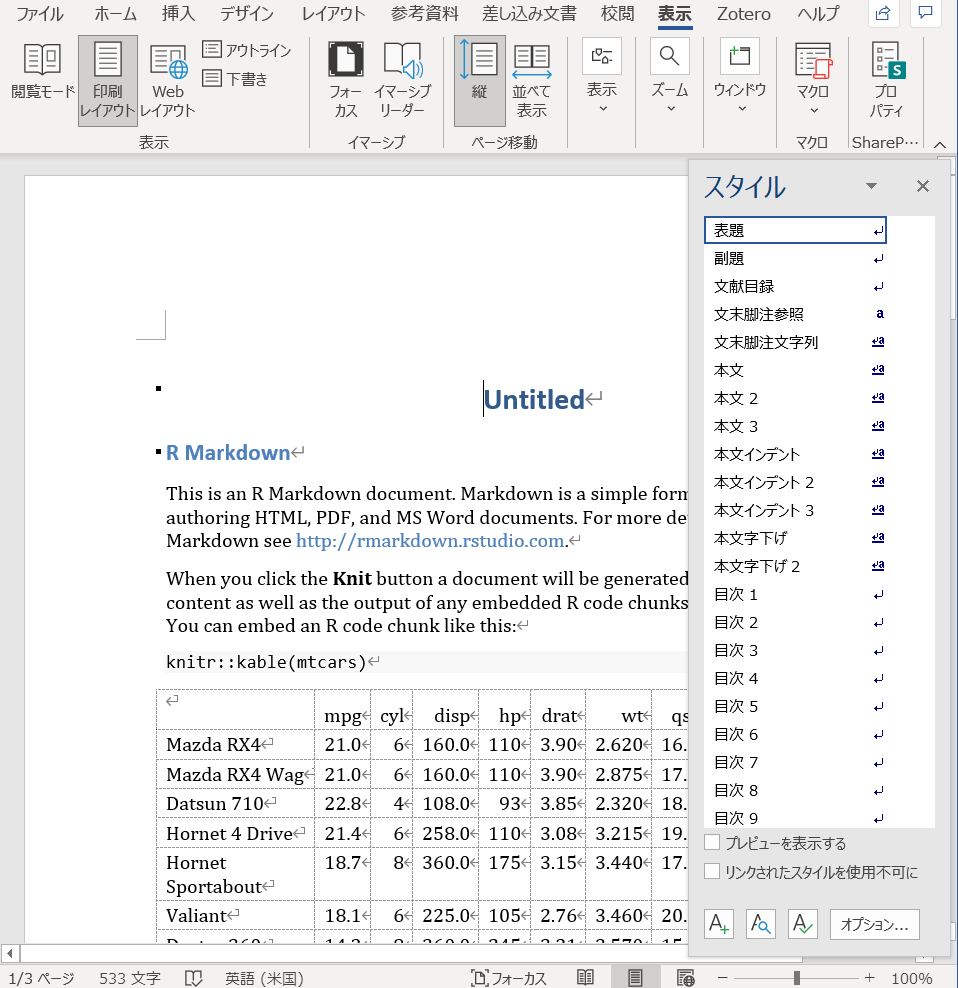
\includegraphics[width=1\linewidth,height=1\textheight,keepaspectratio]{JP/images/word-template-1} 

}

\caption{特定の文書要素のスタイルを見つける}\label{fig:word-template-1}
\end{figure}

図\ref{fig:word-template-1}は Word の「ホーム」タブから ``Styles'' ウィンドウを開くと見つけられます. カーソルを文書の特定の要素上に動かすと, スタイルリストの項目が強調されます. あるタイプの要素のスタイルを変更したいならば, 強調された項目上でドロップダウンメニューをクリックして図\ref{fig:word-template-2}のようなダイアログボックスを見ることができます.

TODO: Word 日本語版での名称確認

\begin{figure}

{\centering 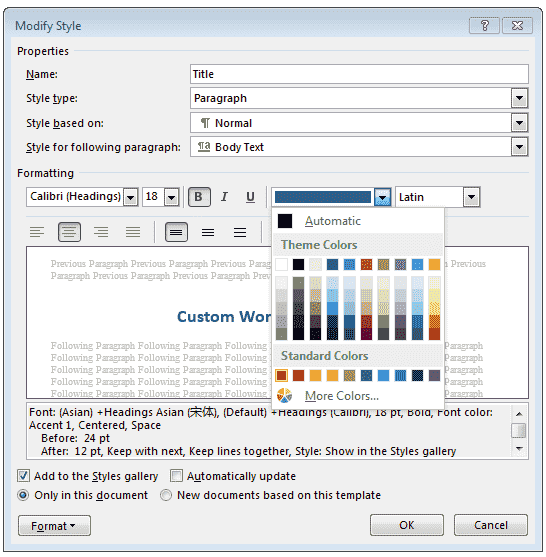
\includegraphics[width=1\linewidth,height=1\textheight,keepaspectratio]{JP/images/word-template-2} 

}

\caption{Word 文書の要素のスタイルを変更する}\label{fig:word-template-2}
\end{figure}

スタイルの編集を終わったら, 文書を保存し (誤って上書きしないようなファイル名にしてください), 今後の Word 文書のテンプレートとして使用することができます. Pandoc が参照文書テンプレートを与えられて新しい Word 文書をレンダリングするとき, テンプレートのスタイルが読み出されそれが新しい文書に適用されます.

カスタムスタイル付きの Word テンプレートを作成する方法の詳細については, \url{https://vimeo.com/110804387} で短い動画を見るか, \url{https://rmarkdown.rstudio.com/articles_docx.html} の記事を読むこともできます.

要素に対するスタイル名がすぐには見つからないこともあるかもしれません. 複数のスタイルが同じ要素に適用され, それらのうち1つだけが強調されてみえることもあるかもしれません. 修正したいスタイルが実際になんであるかは, 当て推量やネット検索で解決することが求められることもあるかもしれません. 例えば ``Manage Styles'' ボタン (図\ref{fig:word-template-1}のスタイルリストの下部にある, 左から3番目のボタン) をクリックし, ``Tabke'' スタイル (図\ref{fig:word-table}参照) を見つけるまでに多数のスタイル名をスクロールして飛ばさなければならりません. これであなたは, 例えば枠線のなどの表のスタイルを修正できます.

\begin{figure}

{\centering 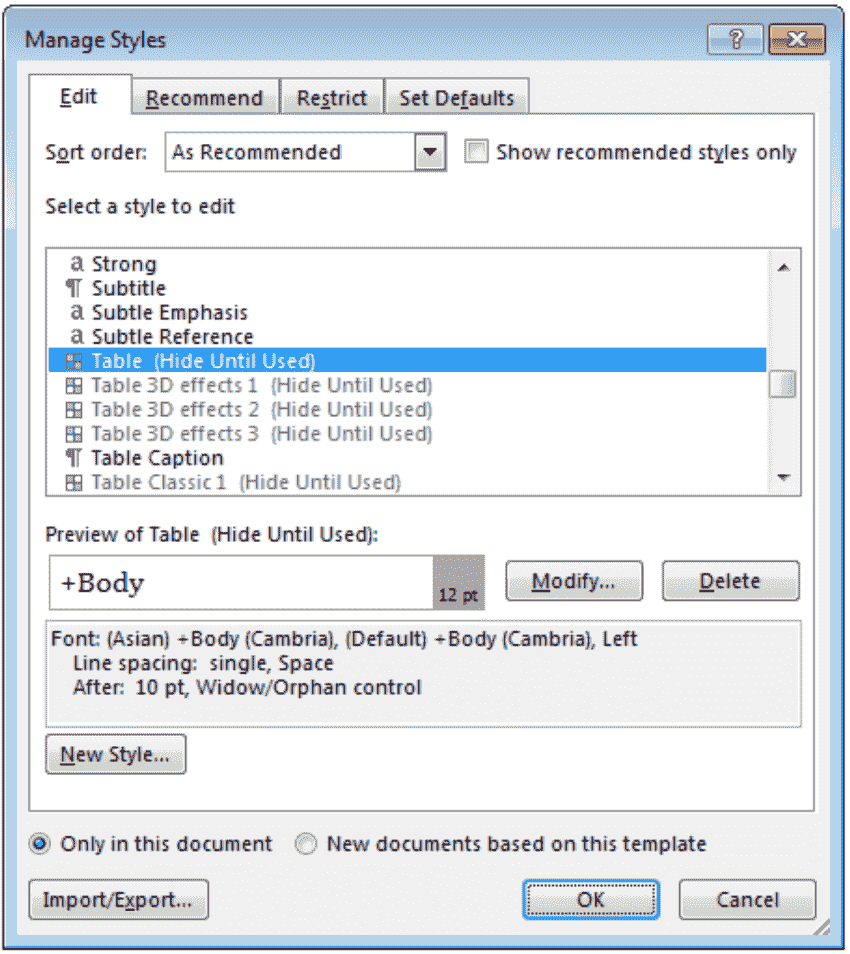
\includegraphics[width=1\linewidth,height=1\textheight,keepaspectratio]{JP/images/word-table} 

}

\caption{Word 文書の表のスタイルを修正する}\label{fig:word-table}
\end{figure}

\hypertarget{word-redoc}{%
\section{R Markdown と Word 間の双方向ワークフロー}\label{word-redoc}}

R Markdown から Word 文書を生成する\index{Word!Rmdとの入出力}のは簡単ですが, 一方で Word 文書を編集して手動の変更を元の R Markdown 文書に反映しなければならないとき, 特に苦痛となるかもしれません. 幸いにも Noam Ross がこの問題に対して有望な解決策を提示しています. \textbf{redoc} パッケージ\index{R パッケージ!redoc} (\url{https://github.com/noamross/redoc}) は Word 文書を生成し, 文書を校正してから R Markdown に再度変換することを可能にします. この原稿を書いている現時点 (2020年6月) では \textbf{redoc} パッケージはまだ試験的であり, さらに不運なことに, 彼は開発を中止しています. どちらにせよこれを試して見たいなら, GitHub からインストールすることができます.

\begin{Shaded}
\begin{Highlighting}[]
\NormalTok{remotes}\SpecialCharTok{::}\FunctionTok{install\_github}\NormalTok{(}\StringTok{"noamross/redoc"}\NormalTok{)}
\end{Highlighting}
\end{Shaded}

パッケージがインストールされたら, 出力フォーマット \texttt{redoc::redoc} を使うこともできます.

\begin{Shaded}
\begin{Highlighting}[]
\PreprocessorTok{{-}{-}{-}}
\FunctionTok{output}\KeywordTok{:}\AttributeTok{ redoc::redoc}
\PreprocessorTok{{-}{-}{-}}
\end{Highlighting}
\end{Shaded}

この出力フォーマットは実質的に元の Rmd 文書を保存している Word 文書を生成するので, Word 文書を Rmd に変換して戻すこともできます. Word 上で追跡された変更箇所は CriticMarkup 構文\index{CriticMarkup} (\url{http://criticmarkup.com}) で書かれたテキストへ変換されます 例えば \texttt{\{++ 重要 ++\}} はテキストに「重要」という単語が挿入されたことを表現しています.

\texttt{redoc::dedoc()} 関数で \texttt{redoc::redoc} で生成された Word 文書を Rmd に変換できます. 例えば \texttt{redoc::dedoc("file.docx")} は \texttt{file.Rmd} を生成します. この処理では Word 上で追跡された変更箇所を \texttt{track\_changes} 引数でどう対処するか決めることができます. 例えば変更を受け入れるか破棄するか, 追跡された変更箇所を CriticMarkup に変換するかなどです. 追跡された変更箇所が完全に失われてしまわないように, \texttt{track\_changes = \textquotesingle{}criticmarkup\textquotesingle{}} を使うことを推奨します.

Word 文書を編集する時, R Markdown のコードチャンクやインライン R コードで自動生成されて\textbf{いない}箇所を編集すると想定されています. 例えばコードチャンク内で \texttt{knitr::kable()} を使って自動生成された表は編集してはなりません. そのような変更は \texttt{dedoc()} で Word から Rmd に変換する際に失われます. コードチャンクで自動生成された出力を誤って編集することを避けるために, \texttt{redoc::redoc} フォーマットの \texttt{highlight\_outputs} オプションを \texttt{true}に設定してください. これは自動出力を Word 上で強調表示することを意味します (背景色で強調表示します). あなたの共同編集者には Word 文書上の強調表示された箇所に触れないよう伝えるべきでしょう.

繰り返しになりますが, \textbf{redoc} パッケージは未だ試験的であり現時点ではその機能がはっきりしないため, ここでの導入はあえて簡潔なものとしています. 信用できない場合, GitHub 上のパッケージのドキュメントを読むことをお薦めします.

TODO: 動作確認

\hypertarget{word-officedown}{%
\section{個別の要素にスタイルを設定する}\label{word-officedown}}

Markdown のシンプルさにより, Word 文書に対してグローバルなスタイル設定を適用することができます (\ref{word-template}節参照) が, ある単語の色やある段落の中央揃えなど, 個別の要素に直接スタイルを設定することはできません.

R 上で Office 文書で作業するのをより簡単にするという努力を続けた結果, David Gohel は 2018 年に \textbf{officedown} パッケージ\index{R パッケージ!officedown} \autocite{R-officedown}の開発を始めました. これは \textbf{officer}\index{R パッケージ!officer} \autocite{R-officer} パッケージの機能のいくつかを R Markdown に持ち込むのが目的です. 本書の執筆時点ではこのパッケージの初期のバージョンが CRAN で公開されていますが, まだ実験的です. CRAN あるいは GitHub どちらからインストールすることもできます.

\begin{Shaded}
\begin{Highlighting}[]
\CommentTok{\# CRAN からインストール}
\FunctionTok{install.packages}\NormalTok{(}\StringTok{"officedown"}\NormalTok{)}

\CommentTok{\# GitHub からインストール}
\NormalTok{remotes}\SpecialCharTok{::}\FunctionTok{install\_github}\NormalTok{(}\StringTok{"davidgohel/officedown"}\NormalTok{)}
\end{Highlighting}
\end{Shaded}

パッケージがインストールされたら, R Markdown 文書内で読み込む必要があります. 例えばこのように.

\begin{Shaded}
\begin{Highlighting}[]
\InformationTok{\textasciigrave{}\textasciigrave{}\textasciigrave{}\{r, setup, include=FALSE\}}
\InformationTok{library(officedown)}
\InformationTok{\textasciigrave{}\textasciigrave{}\textasciigrave{}}
\end{Highlighting}
\end{Shaded}

\textbf{officedown} パッケージには \texttt{rdocx\_document} 出力フォーマットがあります. これはデフォルトでは \texttt{rmarkdown::word\_document} を元にしており, スタイル付きの表やグラフといった機能が追加されています.

\textbf{officedown} パッケージは \textbf{officer} パッケージを介して特定の Word 要素にスタイルを適用することを可能にします. 例えば \texttt{officer::fp\_text()} 関数でスタイルを作成し, インライン R コードの \texttt{ftext()} でテキストの一部にそのスタイルを適用できます.

\begin{Shaded}
\begin{Highlighting}[]
\CommentTok{{-}{-}{-}}
\AnnotationTok{title:}\CommentTok{ officedown でテキストにスタイルを適用する}
\AnnotationTok{output:}
\CommentTok{  officedown::rdocx\_document: default}
\CommentTok{{-}{-}{-}}

\InformationTok{\textasciigrave{}\textasciigrave{}\textasciigrave{}\{r\}}
\InformationTok{library(officedown)}
\InformationTok{library(officer)}
\InformationTok{ft \textless{}{-} fp\_text(color = \textquotesingle{}red\textquotesingle{}, bold = TRUE)}
\InformationTok{\textasciigrave{}\textasciigrave{}\textasciigrave{}}

\FunctionTok{\# テスト}

\NormalTok{**officedown** パッケージは }\InformationTok{\textasciigrave{}r ftext(\textquotesingle{}すごい\textquotesingle{}, ft)\textasciigrave{}}\NormalTok{!}
\end{Highlighting}
\end{Shaded}

\textbf{officer} の関数とは別に, \textbf{officedown} パッケージは \textbf{officer} のタスクを実現するための 特殊な HTML コメントを使うことを可能にしてくれます. 例えば \texttt{officer::block\_pour\_docx()} は外部の Word 文書を現在の文書にインポート\index{Word!外部文書のインポート}するのに使えますし, 代わりに R Markdown 上で HTML コメントを使うこともできます.

\begin{Shaded}
\begin{Highlighting}[]
\CommentTok{\textless{}!{-}{-}{-}BLOCK\_POUR\_DOCX\{file: \textquotesingle{}my{-}file.docx\textquotesingle{}\}{-}{-}{-}\textgreater{}}
\end{Highlighting}
\end{Shaded}

これはインライン R コードで以下のように書くのと等価です.

\begin{Shaded}
\begin{Highlighting}[]
\InformationTok{\textasciigrave{}r block\_pour\_docx(file = \textquotesingle{}my{-}file.docx\textquotesingle{})\textasciigrave{}}
\end{Highlighting}
\end{Shaded}

\textbf{officedown} と \textbf{officer} パッケージでするとよいこととして, 他には以下のようなものがあります.

\begin{itemize}
\item
  改ページの挿入
\item
  多段組みレイアウトの配置
\item
  段落設定の変更
\item
  目次の挿入
\item
  あるセクションのページの向きを変える (縦向きか横向きか)
\end{itemize}

\textbf{officedown} についてより学ぶには, 公式ドキュメント \url{https://davidgohel.github.io/officedown/} を確認してください.

\hypertarget{multi-formats}{%
\chapter{複数の出力フォーマット}\label{multi-formats}}

R Markdown の主な利点は1つのソースから複数種類の出力フォーマットを作成できることです. これは1つ以上の Rmd ファイルでも可能です. 例えば本書は R Markdown で書かれ, 2種類のフォーマットでコンパイルされています. 印刷用の PDF と, オンライン版の HTML です.

コードチャンクの出力を全ての出力フォーマットに対応させるのは時には難題になることがあります. 例えばたった1つの CSS ルール (\texttt{img \{ border-radius: 50\%; \}}) で HTML 出力に対して円の画像を作成するのは非常に単純ですが, LaTeX 出力ではこれとそのまま同じようにはいきません. 典型的には Tikz グラフィックスに関係する問題になります.

単に出力要素が出力フォーマットの全てに対して動作しないこともあります. 例えば \textbf{gifski} パッケージ \autocite{R-gifski} (\ref{animation}節参照) で GIF アニメを簡単に作ることができ, これは HTML 出力では完璧に動作しますが, LaTeX 出力に埋め込んだものは追加の GIF ファイルの処理と LaTeX パッケージなしでは不可能です.

この章では複数のフォーマットで動作する例を少しだけ提示します. ある機能が特定の出力フォーマットでのみ有効なら, その出力形式に基づいて条件付きで有効・無効にする方法を提示します.

\hypertarget{latex-html}{%
\section{LaTeX か HTML か}\label{latex-html}}

LaTeX と HTML はどちらもよく使われるフォーマットです. \texttt{knitr::is\_latex\_output()}\index{knitr!is\_latex\_output()} 関数は出力フォーマットが LaTeX かどうか (Pandoc 出力フォーマットの \texttt{latex} および \texttt{beamer}) を教えてくれます. 同様に \texttt{knitr::is\_html\_output}\index{knitr!is\_html\_output()} 関数は出力フォーマットが HTML かどうか教えてくれます. デフォルトでは Pandoc 出力フォーマットのうち \texttt{markdown}, \texttt{epub}, \texttt{html}, \texttt{html4}, \texttt{html5}, \texttt{revealjs}, \texttt{s5}, \texttt{slideous}, そして \texttt{slidy} が HTML 出力とみなされます. です. ある Pandoc 出力が HTML であると思えないなら, そのフォーマットを除外するために, 例えばこのように \texttt{excludes} 引数を使えます.

\begin{Shaded}
\begin{Highlighting}[numbers=left,,]
\CommentTok{\# markdown を HTML として扱わない}
\NormalTok{knitr}\SpecialCharTok{::}\FunctionTok{is\_html\_output}\NormalTok{(}\AttributeTok{excludes =} \StringTok{"markdown"}\NormalTok{)}
\DocumentationTok{\#\# [1] FALSE}
\end{Highlighting}
\end{Shaded}

特定の出力要素を LaTeX または HTML でのみ生成することができるのなら, これらの関数は条件つきで生成するのに使うことができます. 例えば, PDF のページには大きすぎる表はフォントサイズを小さくした環境内に表を入れるとよいでしょうが, そういった LaTeX 環境はおそらく HTML 出力では機能しませんので, HTML 出力に含めるべきでありません (HTML 出力でフォントサイズを調整したいなら, CSS を使うこともできます). 以下はその例です.

\begin{Shaded}
\begin{Highlighting}[]
\CommentTok{{-}{-}{-}}
\AnnotationTok{title:}\CommentTok{ tiny 環境内で表をレンダリングする}
\AnnotationTok{output:}
\CommentTok{  pdf\_document:}
\CommentTok{    latex\_engine: lualatex}
\CommentTok{  html\_document: default}
\AnnotationTok{documentclass:}\CommentTok{ ltjsarticle}
\CommentTok{{-}{-}{-}}

\InformationTok{\textasciigrave{}\textasciigrave{}\textasciigrave{}\{r, setup, include=FALSE\}}
\InformationTok{knitr::opts\_chunk$set(echo = FALSE)}
\InformationTok{options(knitr.table.format = function() \{}
\InformationTok{  if (knitr::is\_latex\_output()) \textquotesingle{}latex\textquotesingle{} else \textquotesingle{}pandoc\textquotesingle{}}
\InformationTok{\})}
\InformationTok{\textasciigrave{}\textasciigrave{}\textasciigrave{}}

\NormalTok{LaTeX 環境の }\InformationTok{\textasciigrave{}tiny\textasciigrave{}}\NormalTok{ は LaTeX 出力でのみ生成されます.}

\InformationTok{\textasciigrave{}\textasciigrave{}\textasciigrave{}\{r, include=knitr::is\_latex\_output()\}}
\InformationTok{knitr::asis\_output(\textquotesingle{}\textbackslash{}n\textbackslash{}n\textbackslash{}\textbackslash{}begin\{tiny\}\textquotesingle{})}
\InformationTok{\textasciigrave{}\textasciigrave{}\textasciigrave{}}

\InformationTok{\textasciigrave{}\textasciigrave{}\textasciigrave{}\{r\}}
\InformationTok{knitr::kable(mtcars)}
\InformationTok{\textasciigrave{}\textasciigrave{}\textasciigrave{}}

\InformationTok{\textasciigrave{}\textasciigrave{}\textasciigrave{}\{r, include=knitr::is\_latex\_output()\}}
\InformationTok{knitr::asis\_output(\textquotesingle{}\textbackslash{}\textbackslash{}end\{tiny\}\textbackslash{}n\textbackslash{}n\textquotesingle{})}
\InformationTok{\textasciigrave{}\textasciigrave{}\textasciigrave{}}

\NormalTok{比較のため, 以下に通常のフォントサイズの表を配置します.}

\InformationTok{\textasciigrave{}\textasciigrave{}\textasciigrave{}\{r\}}
\InformationTok{knitr::kable(mtcars)}
\InformationTok{\textasciigrave{}\textasciigrave{}\textasciigrave{}}
\end{Highlighting}
\end{Shaded}

上記の例でのポイントはチャンクオプション \texttt{include = knitr::is\_latex\_output()}\index{チャンクオプション!include} です. \texttt{\textbackslash{}begin\{tiny\}\ \textbackslash{}end\{tiny\}} 環境は出力フォーマットが LaTeX の場合のみ含まれます. この例の2つの表は出力が LaTeX でない場合は同じ見た目になるでしょう.

\ref{font-color}節では HTML と LaTeX 出力のテキストの色を変更する関数を使用しました. \ref{animation}節では, アニメーションの例を提示しました. これにも今回のトリックを使うことができます. HTML 出力に対してアニメーションを生成し, LaTeX 出力に対しては静止画を生成するコードチャンクはこのようになります.

\begin{Shaded}
\begin{Highlighting}[]
\InformationTok{\textasciigrave{}\textasciigrave{}\textasciigrave{}\{r animation.hook=if (knitr::is\_html\_output()) \textquotesingle{}gifski\textquotesingle{}\}}
\InformationTok{for (i in 1:2) \{}
\InformationTok{  pie(c(i \%\% 2, 6), col = c(\textquotesingle{}red\textquotesingle{}, \textquotesingle{}yellow\textquotesingle{}), labels = NA)}
\InformationTok{\}}
\InformationTok{\textasciigrave{}\textasciigrave{}\textasciigrave{}}
\end{Highlighting}
\end{Shaded}

これらの条件付き関数はどこでも使えます. 他のチャンクオプションにも使えます (例えばチャンクの評価に条件を付けるため \texttt{eval} に使うなど) し, あるいはこの例のように R コード内にも使えます.

TODO: conditional functions をなんと呼ぶのが良いか

\begin{Shaded}
\begin{Highlighting}[]
\InformationTok{\textasciigrave{}\textasciigrave{}\textasciigrave{}\{r, eval=knitr::is\_html\_output(), echo=FALSE\}}
\InformationTok{cat(\textquotesingle{}これは HTML 出力でのみ見えます\textquotesingle{})}
\InformationTok{\textasciigrave{}\textasciigrave{}\textasciigrave{}}

\InformationTok{\textasciigrave{}\textasciigrave{}\textasciigrave{}\{r\}}
\InformationTok{if (knitr::is\_latex\_output()) \{}
\InformationTok{  knitr::asis\_output(\textquotesingle{}\textbackslash{}n\textbackslash{}n\textbackslash{}\textbackslash{}begin\{tiny\}\textquotesingle{})}
\InformationTok{\}}
\InformationTok{\textasciigrave{}\textasciigrave{}\textasciigrave{}}
\end{Highlighting}
\end{Shaded}

\hypertarget{html-widgets}{%
\section{HTML ウィジェットを表示する}\label{html-widgets}}

HTML ウィジェット (\url{https://htmlwidgets.org})\index{HTML!ウィジェット} は典型例で言えばインタラクティブな JavaScript アプリケーションで, HTML 出力でのみ動作します. HTML ウィジェットを含んだ Rmd 文書を, PDF や Word など HTML でないフォーマットへと knit するなら, このようなエラーメッセージが返ってくるかもしれません.

\begin{Shaded}
\begin{Highlighting}[]
\AnnotationTok{Error:}\CommentTok{ Functions that produce HTML output found in document}
\NormalTok{targeting X output. Please change the output type of this}
\NormalTok{document to HTML. Alternatively, you can allow HTML output in}
\NormalTok{non{-}HTML formats by adding this option to the YAML front{-}matter}
\NormalTok{of your rmarkdown file:}

\NormalTok{  always\_allow\_html: yes}

\NormalTok{Note however that the HTML output will not be visible in}
\NormalTok{non{-}HTML formats.}
\end{Highlighting}
\end{Shaded}

上記のエラーメッセージの方法よりも良い解決法が存在しますが, 追加のパッケージが絡んできます. R に \textbf{webshot} パッケージ\autocite{R-webshot}\index{R パッケージ!webshot} をインストールし, さらに PhantomJS\index{PhantomJS} をインストールしてください.

\begin{Shaded}
\begin{Highlighting}[numbers=left,,]
\FunctionTok{install.packages}\NormalTok{(}\StringTok{"webshot"}\NormalTok{)}
\NormalTok{webshot}\SpecialCharTok{::}\FunctionTok{install\_phantomjs}\NormalTok{()}
\end{Highlighting}
\end{Shaded}

それから HTML ウィジェットつきの Rmd 文書を非 HTML フォーマットで knit すれば, HTML ウィジェットは静的なスクリーンショットとして表示されます. スクリーンショットは \textbf{knitr} によって自動的に作られます. \textbf{bookdown} 本の \href{https://bookdown.org/yihui/bookdown/html-widgets.html}{Section 2.10} に, スクリーンショットの詳しい操作方法が書かれています.

\hypertarget{include-url}{%
\section{Web ページの埋め込み}\label{include-url}}

\textbf{webshot} パッケージ \autocite{R-webshot}\index{R パッケージ!webshot} と PhantomJS\index{PhantomJS} をインストール (\ref{html-widgets}説参照)していれば, \texttt{knitr::include\_url()}\index{knitr!include\_url()} でどんな web ページも出力文書に埋め込むことができます. コードチャンク内でこの関数に URL を与えれば, 出力フォーマットが HTML ならば \texttt{\textless{}iframe\textgreater{}} (インラインフレーム)\index{HTML!iframe} が生成され, 他のパッケージならばスクリーンショットが埋め込まれます. 例えば図\ref{fig:include-url}は, 本書のオンライン版を読んでいるなら私の個人サイトが, それ以外なら代わりに静的なスクリーンショットが現れているはずです.

\let\ooldhref\href
\let\href\oldhref

\begin{Shaded}
\begin{Highlighting}[numbers=left,,]
\NormalTok{knitr}\SpecialCharTok{::}\FunctionTok{include\_url}\NormalTok{(}\StringTok{"https://yihui.org"}\NormalTok{)}
\end{Highlighting}
\end{Shaded}

\begin{figure}

{\centering \oldhref{https://yihui.org}{\includegraphics[width=1\linewidth,height=1\textheight,keepaspectratio]{rmarkdown-cookbook_files/figure-latex/include-url-1} }

}

\caption{iframe または screenshot による Yihui's のホームページ}\label{fig:include-url}
\end{figure}

\let\href\ooldhref

\texttt{out.width} や \texttt{fig.cap} といった図に関連するほとんどのチャンクオプションが \texttt{knitr::include\_url()} でも機能します.

サーバ上で Shiny アプリを公開しているなら, これを文書に含めるために \texttt{knitr::include\_app()}\index{knitr!include\_app()} を使うことができます. これは \texttt{include\_url()} と同じように動作します. \textbf{bookdown} 本 \autocite{bookdown2016} の \href{https://bookdown.org/yihui/bookdown/web-pages-and-shiny-apps.html}{Section 2.11} には \texttt{include\_app()} と \texttt{include\_url()} に関する詳細な話が書かれています.

\hypertarget{figures-side}{%
\section{複数の図を横並びに}\label{figures-side}}

\texttt{fig.show="hold"}\index{チャンクオプション!fig.show} と \texttt{out.width} option\index{チャンクオプション!out.width} オプションを併用して複数の図を並べることができます. 以下の例では \texttt{out.width="48\%"} を設定し, 出力は図\ref{fig:figures-side}になります.

\begin{Shaded}
\begin{Highlighting}[]
\InformationTok{\textasciigrave{}\textasciigrave{}\textasciigrave{}\{r, figures{-}side, fig.show="hold", out.width="48\%"\}}
\InformationTok{par(mar = c(4, 4, .1, .1))}
\InformationTok{plot(cars)}
\InformationTok{plot(mpg \textasciitilde{} hp, data = mtcars, pch = 19)}
\InformationTok{\textasciigrave{}\textasciigrave{}\textasciigrave{}}
\end{Highlighting}
\end{Shaded}

\begin{figure}

{\centering 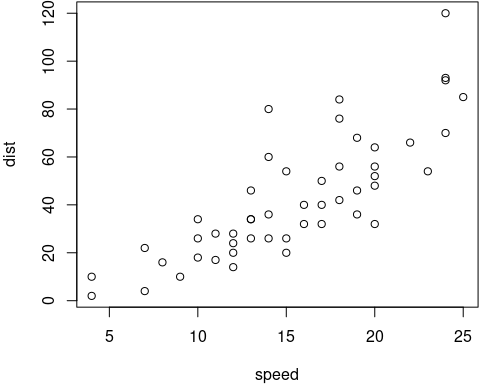
\includegraphics[width=0.48\linewidth,height=1\textheight,keepaspectratio]{rmarkdown-cookbook_files/figure-latex/figures-side-1} 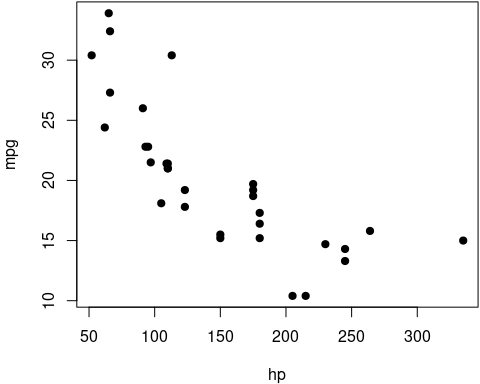
\includegraphics[width=0.48\linewidth,height=1\textheight,keepaspectratio]{rmarkdown-cookbook_files/figure-latex/figures-side-2} 

}

\caption{横に並べた図}\label{fig:figures-side}
\end{figure}

この単純なアプローチは PDF でも HTML 出力でも動作します.

\textbf{訳注}: この方法は, PDF では必ず横並びになるとは限りません. 余白にはみ出す大きさならば, 自動で折り返されます. これは LaTeX 側の文書スタイルの設定にも依存し, 多くの場合は欧文と和文でよく使われるレイアウトが異なることが原因です. よって, ここでは原著とは異なり画像サイズを 48\% と少し小さくしています.

図の内部に複数のプロットがあり, サブフィギュアを使いたいなら, \ref{latex-subfigure}節を見ることができます. しかしサブフィギュアは LaTeX に対してのみのサポートです.

\hypertarget{raw-content}{%
\section{生のコードを書く (*)}\label{raw-content}}

\ref{raw-latex}節で紹介したテクニックは実に汎用的なものです. たどんな複雑な生のコードであっても Markdown 内で「生の」コンテンツとして指定すれば保護されます. 例えば HTML を直接書いたなら, \texttt{=html} 属性を使用することができます.

\begin{Shaded}
\begin{Highlighting}[]
\InformationTok{\textasciigrave{}\textasciigrave{}\textasciigrave{}\{=html\}}
\InformationTok{\textless{}p\textgreater{}どんな\textless{}strong\textgreater{}生の\textless{}/strong\textgreater{} HTML コンテンツでもここでは動作します.}
\InformationTok{例えば, ここにユーチューブのビデオがあります.\textless{}/p\textgreater{}}

\InformationTok{\textless{}iframe width="100\%" height="400"}
\InformationTok{  src="https://www.youtube.com/embed/s3JldKoA0zw?rel=0"}
\InformationTok{  frameborder="0" allow="autoplay; encrypted{-}media"}
\InformationTok{  allowfullscreen\textgreater{}\textless{}/iframe\textgreater{}}
\InformationTok{\textasciigrave{}\textasciigrave{}\textasciigrave{}}
\end{Highlighting}
\end{Shaded}

属性名は Pandoc 出力の名前です. 出力フォーマット名を知りたいなら, Rmd 内で以下のコードチャンクの出力を確認することもできます\index{knitr!pandoc\_toc()}.

\begin{Shaded}
\begin{Highlighting}[]
\InformationTok{\textasciigrave{}\textasciigrave{}\textasciigrave{}\{r\}}
\InformationTok{knitr::pandoc\_to()}
\InformationTok{\textasciigrave{}\textasciigrave{}\textasciigrave{}}
\end{Highlighting}
\end{Shaded}

生のコンテンツは特定の出力フォーマットでのみ表示されることに注意してください. 例えば生の LaTeX コンテンツは出力フォーマットが HTML の場合は無視されます.

\hypertarget{custom-blocks}{%
\section{カスタムブロック (*)}\label{custom-blocks}}

\textbf{bookdown} 本の \href{https://bookdown.org/yihui/bookdown/custom-blocks.html}{2.7節} では, どうすれば R Markdown でブロックの見た目をカスタマイズできるかを話しました. これはレポートや本の中で, 読者があなたの著作の中の要点を確実に取りせるようにコンテンツを目立たせるための, 便利な方法になりうるでしょう. これらのブロックをどう使うかの例として, 次のようなものがあります.

\begin{itemize}
\tightlist
\item
  あなたの分析コードを実行する前に, ユーザが最新のパッケージを使用しているか確認するための警告メッセージを表示する.
\item
  ソースコードのある GitHub リポジトリへのリンクを文書の冒頭に追加する.
\item
  あなたの分析から得られた要点や知見を強調する.
\end{itemize}

この節では PDF と HTML の両方でカスタムブロックを作成する方法を説明します. どちらのフォーマットでも R Markdown 上で同じ整形の構文を使用できますが, 要求される設定は異なります.

\hypertarget{block-syntax}{%
\subsection{構文}\label{block-syntax}}

カスタムブロックの構文は Pandoc の \href{https://pandoc.org/MANUAL.html\#divs-and-spans}{fenced \texttt{Div} blocks} に基づいています. \texttt{Div} ブロック\index{Div}はとても強力ですが1つだけ問題があります. これはおもに HTML 出力に対して動作し, LaTeX 出力に対しては動作しないことです.

バージョン 1.16 以降の \textbf{rmarkdown} パッケージは \texttt{Div} ブロックを HTML と LaTeX どちらに対しても変換するようになりました. HTML 出力に対してはブロックの全ての属性が \texttt{\textless{}div\textgreater{}} タグの属性になります. 例えば \texttt{Div} は ID (\texttt{\#} の後のに続くもの), 1つまたは複数のクラス (クラス名は \texttt{.} の後に書かれるものです), そしてそれ以外の属性を持ちます. 以下の \texttt{Div} ブロック,

\begin{Shaded}
\begin{Highlighting}[]
\NormalTok{::: \{\#hello .greeting .message width="40\%"\}}
\NormalTok{Hello **world**!}
\NormalTok{:::}
\end{Highlighting}
\end{Shaded}

は以下の HTML コードに変換されます.

\begin{Shaded}
\begin{Highlighting}[]
\KeywordTok{\textless{}div}\OtherTok{ id=}\StringTok{"hello"}\OtherTok{ class=}\StringTok{"greeting message"}\OtherTok{ width=}\StringTok{"40\%"}\KeywordTok{\textgreater{}}
\NormalTok{  Hello }\KeywordTok{\textless{}strong\textgreater{}}\NormalTok{world}\KeywordTok{\textless{}/strong\textgreater{}}\NormalTok{!}
\KeywordTok{\textless{}/div\textgreater{}}
\end{Highlighting}
\end{Shaded}

LaTeX 出力に対しては, 最初のクラス名が LaTeX 環境名として使われます. また, \texttt{data-latex}\index{Div!LaTeXとの互換性} と名付けた属性を \texttt{Div} ブロックに与えるべきです. これは環境に対する引数になります. 環境が引数を必要としないなら, この属性は空白にすることができます. 2つの単純な例を以下にお見せします. 1つ目の例は LaTeX で \texttt{verbatim} 環境を使用します. これは引数を必要としません.

\begin{Shaded}
\begin{Highlighting}[]
\NormalTok{::: \{.verbatim data{-}latex=""\}}
\NormalTok{ここに \_verbatim\_ テキストを表示.}
\NormalTok{:::}
\end{Highlighting}
\end{Shaded}

LaTeX 出力はこうなります.

\begin{Shaded}
\begin{Highlighting}[]
\KeywordTok{\textbackslash{}begin}\NormalTok{\{}\ExtensionTok{verbatim}\NormalTok{\}}
\VerbatimStringTok{ここに \textbackslash{}emph\{verbatim\} テキストを表示.}
\KeywordTok{\textbackslash{}end}\NormalTok{\{}\ExtensionTok{verbatim}\NormalTok{\}}
\end{Highlighting}
\end{Shaded}

ブロックが HTML へと変換される場合は, HTML コードはこのようになります.

\begin{Shaded}
\begin{Highlighting}[]
\KeywordTok{\textless{}div}\OtherTok{ class=}\StringTok{"verbatim"}\KeywordTok{\textgreater{}}
\NormalTok{ここに }\KeywordTok{\textless{}em\textgreater{}}\NormalTok{verbatim}\KeywordTok{\textless{}/em\textgreater{}}\NormalTok{ テキストを表示.}
\KeywordTok{\textless{}/div\textgreater{}}
\end{Highlighting}
\end{Shaded}

2つ目の例は \texttt{center} と \texttt{minipage} 環境を使い, ページ幅の半分の大きさの中央揃えしたボックス内にテキストを表示しています.

\begin{Shaded}
\begin{Highlighting}[]
\NormalTok{:::: \{.center data{-}latex=""\}}

\NormalTok{::: \{.minipage data{-}latex="\{.5\textbackslash{}linewidth\}"\}}
\NormalTok{この段落は中央揃えされ, 親要素の半分の幅で表示されます.}
\NormalTok{:::}

\NormalTok{::::}
\end{Highlighting}
\end{Shaded}

\texttt{center} ブロックの中に \texttt{minipage} ブロックをネストしていることに注意してください. 親ブロックに子ブロックを入れるには, さらに1つ余分にコロンが必要です. 上記の例では \texttt{center} ブロックに4つのコロンを使用していますが, 5個以上書くことも可能です. 2つのブロックは以下の LaTeX コードに変換されます.

\begin{Shaded}
\begin{Highlighting}[]
\KeywordTok{\textbackslash{}begin}\NormalTok{\{}\ExtensionTok{center}\NormalTok{\}}
\KeywordTok{\textbackslash{}begin}\NormalTok{\{}\ExtensionTok{minipage}\NormalTok{\}\{.5}\FunctionTok{\textbackslash{}linewidth}\NormalTok{\}}
\NormalTok{この段落は中央揃えされ, 親要素の半分の幅で表示されます.}
\KeywordTok{\textbackslash{}end}\NormalTok{\{}\ExtensionTok{minipage}\NormalTok{\}}
\KeywordTok{\textbackslash{}end}\NormalTok{\{}\ExtensionTok{center}\NormalTok{\}}
\end{Highlighting}
\end{Shaded}

HTML 出力では, ユーザーの好みで CSS によって \texttt{\textless{}div\textgreater{}} ブロックの外見を定義することもできます. LaTeX 出力の場合は, 環境が未定義ならば \texttt{\textbackslash{}newenvironment} を, 既存の環境を再定義するならば \texttt{\textbackslash{}renewenvironment} コマンドを LaTeX 上で使うこともできます. LaTeX 上での定義で PDF 上でのブロックの見た目を決定できます. これらのカスタマイズは通常は \texttt{style.css} や \texttt{preamble.tex} といったファイルを内に記述子, YAML オプションで読み込みます.

\begin{Shaded}
\begin{Highlighting}[]
\PreprocessorTok{{-}{-}{-}}
\FunctionTok{output}\KeywordTok{:}
\AttributeTok{  }\FunctionTok{html\_document}\KeywordTok{:}
\AttributeTok{    }\FunctionTok{css}\KeywordTok{:}\AttributeTok{ style.css}
\AttributeTok{  }\FunctionTok{pdf\_document}\KeywordTok{:}
\AttributeTok{    }\FunctionTok{includes}\KeywordTok{:}
\AttributeTok{      }\FunctionTok{in\_header}\KeywordTok{:}\AttributeTok{ preamble.tex}
\PreprocessorTok{{-}{-}{-}}
\end{Highlighting}
\end{Shaded}

次に, CSS ルールや LaTeX 環境を使用したいくつか発展的なカスタムブロックの実例をお見せします. \ref{multi-column}節にさらなる使用例として, 多段組みレイアウト内で複数ブロックを並べるものがあります.

\hypertarget{block-shaded}{%
\subsection{影付きブロックを追加する}\label{block-shaded}}

まず, 影付きボックスの内部にコンテンツを入れる方法を紹介します. ボックスは黒の背景色とオレンジ色の枠があり, 角は丸めます. ボックス内のテキストは白色です.

HTML 出力に対しては, CSS ファイル内でそのルールを定義します. CSS\index{CSS}にあまり詳しくないなくても, 無料で見られるオンラインチュートリアルが豊富にあります. 例えば \url{https://www.w3schools.com/css/} とか.

TODO: 日本語の代替サイト

\begin{Shaded}
\begin{Highlighting}[numbers=left,,]
\FunctionTok{.blackbox}\NormalTok{ \{}
  \KeywordTok{padding}\NormalTok{: }\DecValTok{1}\DataTypeTok{em}\OperatorTok{;}
  \KeywordTok{background}\NormalTok{: }\ConstantTok{black}\OperatorTok{;}
  \KeywordTok{color}\NormalTok{: }\ConstantTok{white}\OperatorTok{;}
  \KeywordTok{border}\NormalTok{: }\DecValTok{2}\DataTypeTok{px} \DecValTok{solid} \ConstantTok{orange}\OperatorTok{;}
  \KeywordTok{border{-}radius}\NormalTok{: }\DecValTok{10}\DataTypeTok{px}\OperatorTok{;}
\NormalTok{\}}
\FunctionTok{.center}\NormalTok{ \{}
  \KeywordTok{text{-}align}\NormalTok{: }\DecValTok{center}\OperatorTok{;}
\NormalTok{\}}
\end{Highlighting}
\end{Shaded}

LaTeX 出力に対しては, LaTeX パッケージの \textbf{framed}\index{LaTeX パッケージ!framed} を基にして \texttt{blackbox} という名前で黒い背景色と白い文字色の新しい環境を作成します.

\begin{Shaded}
\begin{Highlighting}[numbers=left,,]
\BuiltInTok{\textbackslash{}usepackage}\NormalTok{\{}\ExtensionTok{color}\NormalTok{\}}
\BuiltInTok{\textbackslash{}usepackage}\NormalTok{\{}\ExtensionTok{framed}\NormalTok{\}}
\FunctionTok{\textbackslash{}setlength}\NormalTok{\{}\FunctionTok{\textbackslash{}fboxsep}\NormalTok{\}\{.8em\}}

\FunctionTok{\textbackslash{}newenvironment}\NormalTok{\{blackbox\}\{}
  \FunctionTok{\textbackslash{}definecolor}\NormalTok{\{shadecolor\}\{rgb\}\{0, 0, 0\}  }\CommentTok{\% black}
  \FunctionTok{\textbackslash{}color}\NormalTok{\{white\}}
  \KeywordTok{\textbackslash{}begin}\NormalTok{\{}\ExtensionTok{shaded}\NormalTok{\}\}}
\NormalTok{ \{}\KeywordTok{\textbackslash{}end}\NormalTok{\{}\ExtensionTok{shaded}\NormalTok{\}\}}
\end{Highlighting}
\end{Shaded}

本書で \textbf{framed} パッケージを使うのはこれがかなり軽量だからですが, このパッケージは角の丸い枠を描画することができません. それを実現するには, 影付きボックスを作るためのとても柔軟な一連のオプションを持つ, より洗練された LaTeX パッケージである \textbf{tcolorblox} (\url{https://ctan.org/pkg/tcolorbox})\index{LaTeX パッケージ!tcolorbox}が必要になります. パッケージのドキュメントからは多くの使用例を見ることができます. 以下の LaTeX 環境は上記の CSS の例と似た影付きボックスを作成できます.

\begin{Shaded}
\begin{Highlighting}[]
\BuiltInTok{\textbackslash{}usepackage}\NormalTok{\{}\ExtensionTok{tcolorbox}\NormalTok{\}}

\FunctionTok{\textbackslash{}newtcolorbox}\NormalTok{\{blackbox\}\{}
\NormalTok{  colback=black,}
\NormalTok{  colframe=orange,}
\NormalTok{  coltext=white,}
\NormalTok{  boxsep=5pt,}
\NormalTok{  arc=4pt\}}
\end{Highlighting}
\end{Shaded}

これで PDF と HTML 出力の両方のフォーマットでカスタムボックスを使用できるようになりました. ボックスのソースコードはこのようになります.

\begin{Shaded}
\begin{Highlighting}[]
\NormalTok{:::: \{.blackbox data{-}latex=""\}}
\NormalTok{::: \{.center data{-}latex=""\}}
\NormalTok{**注意!**}
\NormalTok{:::}

\NormalTok{この**新しい注意書き**を見てくれてありがとう! あなたがこれを見ていることは監視されており, 当局に報告される!}
\NormalTok{::::}
\end{Highlighting}
\end{Shaded}

出力は:

\begin{blackbox}

\begin{center}
\textbf{注意!}

\end{center}

この\textbf{新しい注意書き}を見てくれてありがとう! あなたがこれを見ていることは監視されており, 当局に報告される!

\end{blackbox}

\hypertarget{block-image}{%
\subsection{アイコンを加える}\label{block-image}}

カスタムボックス内に画像を含めることで, より注意を引く見た目に作ることができます. 画像はブロックの内容をより効果的に伝える方法にもなりえます. 次の例は, このようなディレクトリ構造で動作させるという前提です. これは本書を作成するために使ったものを簡略化したものです.

\begin{verbatim}
directory/
├── your-report.Rmd
├── style.css
├── preamble.tex
└── images/ 
      └── ├── important.png
          ├── note.png
          └── caution.png
\end{verbatim}

どのように動作するか説明する前に, この例のソースコードと出力を示します.

\begin{Shaded}
\begin{Highlighting}[]
\NormalTok{::: \{.infobox .caution data{-}latex="\{caution\}"\}}
\NormalTok{**注意!**}

\NormalTok{この**新しい注意書き**を見てくれてありがとう! あなたがこれを見ていることは監視されており, 当局に報告される!}
\NormalTok{:::}
\end{Highlighting}
\end{Shaded}

出力はこうなります.

\begin{infobox}{caution}
\textbf{注意!}

この\textbf{新しい注意書き}を見てくれてありがとう! あなたがこれを見ていることは監視されており, 当局に報告される!

\end{infobox}

HTML 出力では, CSS の \texttt{background-image}\index{CSS プロパティ!background-image} プロパティ内にボックスの画像を追加することができます. 背景に画像を挿入し, 左側に十分な幅のパディングを追加することでテキストと画像の重なりを避けます. ローカルの画像ファイルを使用するなら, ファイルパスは CSS との相対パスで与えます. これが例です.

\begin{Shaded}
\begin{Highlighting}[]
\FunctionTok{.infobox}\NormalTok{ \{}
  \KeywordTok{padding}\NormalTok{: }\DecValTok{1}\DataTypeTok{em} \DecValTok{1}\DataTypeTok{em} \DecValTok{1}\DataTypeTok{em} \DecValTok{4}\DataTypeTok{em}\OperatorTok{;}
  \KeywordTok{margin{-}bottom}\NormalTok{: }\DecValTok{10}\DataTypeTok{px}\OperatorTok{;}
  \KeywordTok{border}\NormalTok{: }\DecValTok{2}\DataTypeTok{px} \DecValTok{solid} \ConstantTok{orange}\OperatorTok{;}
  \KeywordTok{border{-}radius}\NormalTok{: }\DecValTok{10}\DataTypeTok{px}\OperatorTok{;}
  \KeywordTok{background}\NormalTok{: }\ConstantTok{\#f5f5f5} \DecValTok{5}\DataTypeTok{px} \DecValTok{center}\NormalTok{/}\DecValTok{3}\DataTypeTok{em} \DecValTok{no{-}repeat}\OperatorTok{;}
\NormalTok{\}}

\FunctionTok{.caution}\NormalTok{ \{}
  \KeywordTok{background{-}image}\NormalTok{: }\FunctionTok{url(}\StringTok{"images/caution.png"}\FunctionTok{)}\OperatorTok{;}
\NormalTok{\}}
\end{Highlighting}
\end{Shaded}

ブロックに \texttt{.infobox} と \texttt{.caution} という2つのクラス名を使用していることに注意してください. \texttt{infobox} クラスは色付きの外枠のある影付きボックスを定義するのに使用し, \texttt{caution} クラスは画像を入れるために使用されています. 2つのクラスを使用する利点は影付きボックスの設定を繰り返すことなく, いろいろなアイコンの付いたブロックを定義できるということです. \texttt{warning} のボックスが必要ならば, \texttt{.infobox} のルールを繰り返し書くことなく, 以下のように定義するだけで十分です.

\begin{Shaded}
\begin{Highlighting}[]
\FunctionTok{.warning}\NormalTok{ \{}
  \KeywordTok{background{-}image}\NormalTok{: }\FunctionTok{url(}\StringTok{"images/warning.png"}\FunctionTok{)}\OperatorTok{;}
\NormalTok{\}}
\end{Highlighting}
\end{Shaded}

すると以下の Markdown ソースコードで \texttt{warning} ボックスを作成できます.

\begin{Shaded}
\begin{Highlighting}[]
\NormalTok{:::: \{.infobox .warning data{-}latex="warning"\}}

\NormalTok{実際のコンテンツをここに表示}

\NormalTok{::::}
\end{Highlighting}
\end{Shaded}

PDF 出力に対しては, 以前の例で定義した \texttt{blackbox} 環境を基に \texttt{infobox} 環境を作成し, ボックスの左側に画像を追加できます. LaTeX 環境に画像を追加する方法はいくつもあります. これはそのうちの1つにすぎません. なお, これは上記の CSS で定義したスタイルを正確に再現するものではありません.

\begin{Shaded}
\begin{Highlighting}[numbers=left,,]
\FunctionTok{\textbackslash{}newenvironment}\NormalTok{\{infobox\}[1]}
\NormalTok{  \{}
  \KeywordTok{\textbackslash{}begin}\NormalTok{\{}\ExtensionTok{itemize}\NormalTok{\}}
  \FunctionTok{\textbackslash{}renewcommand}\NormalTok{\{}\ExtensionTok{\textbackslash{}labelitemi}\NormalTok{\}\{}
    \FunctionTok{\textbackslash{}raisebox}\NormalTok{\{{-}.7}\FunctionTok{\textbackslash{}height}\NormalTok{\}[0pt][0pt]\{}
\NormalTok{      \{}\FunctionTok{\textbackslash{}setkeys}\NormalTok{\{Gin\}\{width=3em,keepaspectratio\}}
        \BuiltInTok{\textbackslash{}includegraphics}\NormalTok{\{}\ExtensionTok{images/\#1}\NormalTok{\}\}}
\NormalTok{    \}}
\NormalTok{  \}}
  \FunctionTok{\textbackslash{}setlength}\NormalTok{\{}\FunctionTok{\textbackslash{}fboxsep}\NormalTok{\}\{1em\}}
  \KeywordTok{\textbackslash{}begin}\NormalTok{\{}\ExtensionTok{blackbox}\NormalTok{\}}
  \FunctionTok{\textbackslash{}item}
\NormalTok{  \}}
\NormalTok{  \{}
  \KeywordTok{\textbackslash{}end}\NormalTok{\{}\ExtensionTok{blackbox}\NormalTok{\}}
  \KeywordTok{\textbackslash{}end}\NormalTok{\{}\ExtensionTok{itemize}\NormalTok{\}}
\NormalTok{  \}}
\end{Highlighting}
\end{Shaded}

以下に, 異なるアイコンでブロックを示します. Below we show more example blocks with different icons:

\begin{infobox}{warning}
\textbf{注意!}

この\textbf{新しい注意書き}を見てくれてありがとう! あなたがこれを見ていることは監視されており, 当局に報告される!

\end{infobox}

\begin{infobox}{note}
\textbf{注意!}

この\textbf{新しい注意書き}を見てくれてありがとう! あなたがこれを見ていることは監視されており, 当局に報告される!

\end{infobox}

\begin{infobox}{important}
\textbf{注意!}

この\textbf{新しい注意書き}を見てくれてありがとう! あなたがこれを見ていることは監視されており, 当局に報告される!

\end{infobox}

\begin{infobox}{tip}
\textbf{注意!}

この\textbf{新しい注意書き}を見てくれてありがとう! あなたがこれを見ていることは監視されており, 当局に報告される!

\end{infobox}

代替案として, LaTeX パッケージの \href{https://ctan.org/pkg/awesomebox}{\textbf{awesomebox}}\index{LaTeX パッケージ!awesomebox} を使って PDF にアイコン付きのボックスを生成することもできます. このパッケージがあれば非常に多くのアイコンを選ぶことができます. 以下に簡単な例をお見せします. 使用可能な LaTeX 環境と引数についてはパッケージのドキュメントを参照してください.

\begin{Shaded}
\begin{Highlighting}[]
\CommentTok{{-}{-}{-}}
\AnnotationTok{title:}\CommentTok{ Awesome Boxes}
\AnnotationTok{output:}
\CommentTok{  pdf\_document:}
\CommentTok{    latex\_engine: lualatex}
\CommentTok{    extra\_dependencies: awesomebox}
\AnnotationTok{documentlass:}\CommentTok{ ltjsarticle}
\AnnotationTok{mainfont:}\CommentTok{ Noto Serif CJK JP}
\AnnotationTok{sansfont:}\CommentTok{ Noto Sans CJK JP}
\CommentTok{{-}{-}{-}}

\NormalTok{"note" 型のボックス:}

\NormalTok{::: \{.noteblock data{-}latex=""\}}
\NormalTok{この**新しい注意書き**を見てくれてありがとう! あなたがこれを見ていることは監視されており, あなたがこれを見ていることは監視されており, \_当局に報告される\_!}
\NormalTok{:::}

\NormalTok{このボックスの引数を生成するための R 関数 }\InformationTok{\textasciigrave{}box\_args()\textasciigrave{}}\NormalTok{ を定義しました.}

\InformationTok{\textasciigrave{}\textasciigrave{}\textasciigrave{}\{r\}}
\InformationTok{box\_args \textless{}{-} function(}
\InformationTok{  vrulecolor = \textquotesingle{}white\textquotesingle{},}
\InformationTok{  hrule = c(\textquotesingle{}\textbackslash{}\textbackslash{}abLongLine\textquotesingle{}, \textquotesingle{}\textbackslash{}\textbackslash{}abShortLine\textquotesingle{}, \textquotesingle{}\textquotesingle{}),}
\InformationTok{  title = \textquotesingle{}\textquotesingle{}, vrulewidth = \textquotesingle{}0pt\textquotesingle{},}
\InformationTok{  icon = \textquotesingle{}Bomb\textquotesingle{}, iconcolor = \textquotesingle{}black\textquotesingle{}}
\InformationTok{) \{}
\InformationTok{  hrule \textless{}{-} match.arg(hrule)}
\InformationTok{  sprintf(}
\InformationTok{    \textquotesingle{}[\%s][\%s][\textbackslash{}\textbackslash{}textbf\{\%s\}]\{\%s\}\{\textbackslash{}\textbackslash{}fa\%s\}\{\%s\}\textquotesingle{},}
\InformationTok{    vrulecolor, hrule, title, vrulewidth, icon, iconcolor}
\InformationTok{  )}
\InformationTok{\}}
\InformationTok{\textasciigrave{}\textasciigrave{}\textasciigrave{}}

\NormalTok{インライン R コード内で }\InformationTok{\textasciigrave{}awesomeblock\textasciigrave{}}\NormalTok{ 環境に引数を与えます.}

\NormalTok{::: \{.awesomeblock data{-}latex="}\InformationTok{\textasciigrave{}r box\_args(title = \textquotesingle{}注意!\textquotesingle{})\textasciigrave{}}\NormalTok{"\}}
\NormalTok{この**新しい注意書き**を見てくれてありがとう!}

\NormalTok{あなたがこれを見ていることは監視されており, \_当局に報告される\_!}
\NormalTok{:::}
\end{Highlighting}
\end{Shaded}

\textbf{訳注}: 翻訳者の開発した \textbf{rmdja} パッケージでは, デフォルトでこの節で紹介されているようなカスタムブロックが定義されており, より簡単にアイコン付きブロックを記述できます. 詳細はこのパッケージのドキュメントをご覧ください.

\hypertarget{tables}{%
\chapter{表}\label{tables}}

表は, レポート上で結果を伝えることができる主要な手段です. 表をあなたの独自の要件に合った外見に調整したいと思うことはしばしばあるでしょう. この章では表のカスタマイズに使えるテクニックを紹介します. この章のねらいは以下のとおりです.

\begin{itemize}
\tightlist
\item
  表生成関数 \texttt{knitr::kable()} の全ての特徴を紹介する
\item
  \textbf{kableExtra} パッケージ \autocite{R-kableExtra} を使用したより発展的な表のカスタマイズに焦点を当てる
\item
  表を生成してくれる他のパッケージの一覧を提示する
\end{itemize}

\hypertarget{kable}{%
\section{\texorpdfstring{\texttt{knitr::kable()} 関数}{knitr::kable() 関数}}\label{kable}}

\textbf{knitr} パッケージの \texttt{kable()}\index{knitr!kable()} 関数はとてもシンプルな表生成用の関数で, 表のデザインもシンプルです. 行列やデータフレーム厳密に矩形状のデータに対してのみ表を生成します. 表のセルを細かく整形したりセルを結合したりはできません. しかしこの関数は表の外見をカスタマイズする多くの引数を持っています.

\begin{Shaded}
\begin{Highlighting}[numbers=left,,]
\FunctionTok{kable}\NormalTok{(x, format, }\AttributeTok{digits =} \FunctionTok{getOption}\NormalTok{(}\StringTok{"digits"}\NormalTok{), }\AttributeTok{row.names =} \ConstantTok{NA}\NormalTok{, }
  \AttributeTok{col.names =} \ConstantTok{NA}\NormalTok{, align, }\AttributeTok{caption =} \ConstantTok{NULL}\NormalTok{, }\AttributeTok{label =} \ConstantTok{NULL}\NormalTok{, }
  \AttributeTok{format.args =} \FunctionTok{list}\NormalTok{(), }\AttributeTok{escape =} \ConstantTok{TRUE}\NormalTok{, ...)}
\end{Highlighting}
\end{Shaded}

\hypertarget{kable-formats}{%
\subsection{サポートする表形式}\label{kable-formats}}

データオブジェクト \texttt{x} を単純な表で表すことだけが必要ならば, ほとんどの場合, \texttt{knitr::kable(x)} で十分でしょう. \texttt{format} 引数は \textbf{knitr} のソース文書フォーマットに従って自動的に設定されます. 使用可能な値は列をパイプで区切った \texttt{pipe}, Pandoc 式の単純な表である \texttt{simple}, LaTeX の表 \texttt{latex}, HTML の表 \texttt{html}, reStructuredText (rst) 形式の \texttt{rst} です. R Markdown 文書に対して \texttt{kable()} はデフォルトで \texttt{pipe} フォーマットを使用し, このような外見になります.

\begin{Shaded}
\begin{Highlighting}[numbers=left,,]
\NormalTok{knitr}\SpecialCharTok{::}\FunctionTok{kable}\NormalTok{(}\FunctionTok{head}\NormalTok{(mtcars[, }\DecValTok{1}\SpecialCharTok{:}\DecValTok{4}\NormalTok{]), }\StringTok{"pipe"}\NormalTok{)}
\end{Highlighting}
\end{Shaded}

\begin{Shaded}
\begin{Highlighting}[]
\NormalTok{|                  |  mpg| cyl| disp|  hp|}
\NormalTok{|:{-}{-}{-}{-}{-}{-}{-}{-}{-}{-}{-}{-}{-}{-}{-}{-}{-}|{-}{-}{-}{-}:|{-}{-}{-}:|{-}{-}{-}{-}:|{-}{-}{-}:|}
\NormalTok{|Mazda RX4         | 21.0|   6|  160| 110|}
\NormalTok{|Mazda RX4 Wag     | 21.0|   6|  160| 110|}
\NormalTok{|Datsun 710        | 22.8|   4|  108|  93|}
\NormalTok{|Hornet 4 Drive    | 21.4|   6|  258| 110|}
\NormalTok{|Hornet Sportabout | 18.7|   8|  360| 175|}
\NormalTok{|Valiant           | 18.1|   6|  225| 105|}
\end{Highlighting}
\end{Shaded}

単純な表, そして HTML, LaTeX, reStructuredText での表を生成できます. You can also generate simple tables, or tables in HTML, LaTeX, and reStructuredText:

\begin{Shaded}
\begin{Highlighting}[numbers=left,,]
\NormalTok{knitr}\SpecialCharTok{::}\FunctionTok{kable}\NormalTok{(}\FunctionTok{head}\NormalTok{(mtcars[, }\DecValTok{1}\SpecialCharTok{:}\DecValTok{4}\NormalTok{]), }\StringTok{"simple"}\NormalTok{)}
\end{Highlighting}
\end{Shaded}

\begin{Shaded}
\begin{Highlighting}[]
\InformationTok{                      mpg   cyl   disp    hp}
\NormalTok{{-}{-}{-}{-}{-}{-}{-}{-}{-}{-}{-}{-}{-}{-}{-}{-}{-}{-}  {-}{-}{-}{-}{-}  {-}{-}{-}{-}  {-}{-}{-}{-}{-}  {-}{-}{-}{-}}
\NormalTok{Mazda RX4            21.0     6    160   110}
\NormalTok{Mazda RX4 Wag        21.0     6    160   110}
\NormalTok{Datsun 710           22.8     4    108    93}
\NormalTok{Hornet 4 Drive       21.4     6    258   110}
\NormalTok{Hornet Sportabout    18.7     8    360   175}
\NormalTok{Valiant              18.1     6    225   105}
\end{Highlighting}
\end{Shaded}

\begin{Shaded}
\begin{Highlighting}[numbers=left,,]
\NormalTok{knitr}\SpecialCharTok{::}\FunctionTok{kable}\NormalTok{(mtcars[}\DecValTok{1}\SpecialCharTok{:}\DecValTok{2}\NormalTok{, }\DecValTok{1}\SpecialCharTok{:}\DecValTok{2}\NormalTok{], }\StringTok{"html"}\NormalTok{)}
\end{Highlighting}
\end{Shaded}

\begin{Shaded}
\begin{Highlighting}[]
\KeywordTok{\textless{}table\textgreater{}}
 \KeywordTok{\textless{}thead\textgreater{}}
  \KeywordTok{\textless{}tr\textgreater{}}
   \KeywordTok{\textless{}th}\OtherTok{ style=}\StringTok{"text{-}align:left;"}\KeywordTok{\textgreater{}}   \KeywordTok{\textless{}/th\textgreater{}}
   \KeywordTok{\textless{}th}\OtherTok{ style=}\StringTok{"text{-}align:right;"}\KeywordTok{\textgreater{}}\NormalTok{ mpg }\KeywordTok{\textless{}/th\textgreater{}}
   \KeywordTok{\textless{}th}\OtherTok{ style=}\StringTok{"text{-}align:right;"}\KeywordTok{\textgreater{}}\NormalTok{ cyl }\KeywordTok{\textless{}/th\textgreater{}}
  \KeywordTok{\textless{}/tr\textgreater{}}
 \KeywordTok{\textless{}/thead\textgreater{}}
\KeywordTok{\textless{}tbody\textgreater{}}
  \KeywordTok{\textless{}tr\textgreater{}}
   \KeywordTok{\textless{}td}\OtherTok{ style=}\StringTok{"text{-}align:left;"}\KeywordTok{\textgreater{}}\NormalTok{ Mazda RX4 }\KeywordTok{\textless{}/td\textgreater{}}
   \KeywordTok{\textless{}td}\OtherTok{ style=}\StringTok{"text{-}align:right;"}\KeywordTok{\textgreater{}}\NormalTok{ 21 }\KeywordTok{\textless{}/td\textgreater{}}
   \KeywordTok{\textless{}td}\OtherTok{ style=}\StringTok{"text{-}align:right;"}\KeywordTok{\textgreater{}}\NormalTok{ 6 }\KeywordTok{\textless{}/td\textgreater{}}
  \KeywordTok{\textless{}/tr\textgreater{}}
  \KeywordTok{\textless{}tr\textgreater{}}
   \KeywordTok{\textless{}td}\OtherTok{ style=}\StringTok{"text{-}align:left;"}\KeywordTok{\textgreater{}}\NormalTok{ Mazda RX4 Wag }\KeywordTok{\textless{}/td\textgreater{}}
   \KeywordTok{\textless{}td}\OtherTok{ style=}\StringTok{"text{-}align:right;"}\KeywordTok{\textgreater{}}\NormalTok{ 21 }\KeywordTok{\textless{}/td\textgreater{}}
   \KeywordTok{\textless{}td}\OtherTok{ style=}\StringTok{"text{-}align:right;"}\KeywordTok{\textgreater{}}\NormalTok{ 6 }\KeywordTok{\textless{}/td\textgreater{}}
  \KeywordTok{\textless{}/tr\textgreater{}}
\KeywordTok{\textless{}/tbody\textgreater{}}
\KeywordTok{\textless{}/table\textgreater{}}
\end{Highlighting}
\end{Shaded}

\begin{Shaded}
\begin{Highlighting}[numbers=left,,]
\NormalTok{knitr}\SpecialCharTok{::}\FunctionTok{kable}\NormalTok{(}\FunctionTok{head}\NormalTok{(mtcars[, }\DecValTok{1}\SpecialCharTok{:}\DecValTok{4}\NormalTok{]), }\StringTok{"latex"}\NormalTok{)}
\end{Highlighting}
\end{Shaded}

\begin{Shaded}
\begin{Highlighting}[]
\KeywordTok{\textbackslash{}begin}\NormalTok{\{}\ExtensionTok{tabular}\NormalTok{\}\{l|r|r|r|r\}}
\FunctionTok{\textbackslash{}hline}
  \OperatorTok{\&}\NormalTok{ mpg }\OperatorTok{\&}\NormalTok{ cyl }\OperatorTok{\&}\NormalTok{ disp }\OperatorTok{\&}\NormalTok{ hp}\FunctionTok{\textbackslash{}\textbackslash{}}
\FunctionTok{\textbackslash{}hline}
\NormalTok{Mazda RX4 }\OperatorTok{\&}\NormalTok{ 21.0 }\OperatorTok{\&}\NormalTok{ 6 }\OperatorTok{\&}\NormalTok{ 160 }\OperatorTok{\&}\NormalTok{ 110}\FunctionTok{\textbackslash{}\textbackslash{}}
\FunctionTok{\textbackslash{}hline}
\NormalTok{Mazda RX4 Wag }\OperatorTok{\&}\NormalTok{ 21.0 }\OperatorTok{\&}\NormalTok{ 6 }\OperatorTok{\&}\NormalTok{ 160 }\OperatorTok{\&}\NormalTok{ 110}\FunctionTok{\textbackslash{}\textbackslash{}}
\FunctionTok{\textbackslash{}hline}
\NormalTok{Datsun 710 }\OperatorTok{\&}\NormalTok{ 22.8 }\OperatorTok{\&}\NormalTok{ 4 }\OperatorTok{\&}\NormalTok{ 108 }\OperatorTok{\&}\NormalTok{ 93}\FunctionTok{\textbackslash{}\textbackslash{}}
\FunctionTok{\textbackslash{}hline}
\NormalTok{Hornet 4 Drive }\OperatorTok{\&}\NormalTok{ 21.4 }\OperatorTok{\&}\NormalTok{ 6 }\OperatorTok{\&}\NormalTok{ 258 }\OperatorTok{\&}\NormalTok{ 110}\FunctionTok{\textbackslash{}\textbackslash{}}
\FunctionTok{\textbackslash{}hline}
\NormalTok{Hornet Sportabout }\OperatorTok{\&}\NormalTok{ 18.7 }\OperatorTok{\&}\NormalTok{ 8 }\OperatorTok{\&}\NormalTok{ 360 }\OperatorTok{\&}\NormalTok{ 175}\FunctionTok{\textbackslash{}\textbackslash{}}
\FunctionTok{\textbackslash{}hline}
\NormalTok{Valiant }\OperatorTok{\&}\NormalTok{ 18.1 }\OperatorTok{\&}\NormalTok{ 6 }\OperatorTok{\&}\NormalTok{ 225 }\OperatorTok{\&}\NormalTok{ 105}\FunctionTok{\textbackslash{}\textbackslash{}}
\FunctionTok{\textbackslash{}hline}
\KeywordTok{\textbackslash{}end}\NormalTok{\{}\ExtensionTok{tabular}\NormalTok{\}}
\end{Highlighting}
\end{Shaded}

\begin{Shaded}
\begin{Highlighting}[numbers=left,,]
\NormalTok{knitr}\SpecialCharTok{::}\FunctionTok{kable}\NormalTok{(}\FunctionTok{head}\NormalTok{(mtcars[, }\DecValTok{1}\SpecialCharTok{:}\DecValTok{4}\NormalTok{]), }\StringTok{"rst"}\NormalTok{)}
\end{Highlighting}
\end{Shaded}

\begin{Shaded}
\begin{Highlighting}[]
\NormalTok{=================  ====  ===  ====  ===}
\NormalTok{\textbackslash{}                   mpg  cyl  disp   hp}
\NormalTok{=================  ====  ===  ====  ===}
\NormalTok{Mazda RX4          21.0    6   160  110}
\NormalTok{Mazda RX4 Wag      21.0    6   160  110}
\NormalTok{Datsun 710         22.8    4   108   93}
\NormalTok{Hornet 4 Drive     21.4    6   258  110}
\NormalTok{Hornet Sportabout  18.7    8   360  175}
\NormalTok{Valiant            18.1    6   225  105}
\NormalTok{=================  ====  ===  ====  ===}
\end{Highlighting}
\end{Shaded}

\texttt{pipe} と \texttt{simple} のフォーマットのみが移植可能だと覚えておいてください. つまり, これらだけがいずれの出力文書フォーマットでも動作します. それ以外の表形式は特定のフォーマットに対してのみ, 例えば \texttt{format = \textquotesingle{}latex\textquotesingle{}} は LaTeX 出力に対してのみの動作です. 移植性を犠牲にする代わりに, 特定の表形式を使うことでより細かい操作ができます.

特定の1つの表形式だけが必要で, それが文書のデフォルト形式でないなら, \texttt{knitr.table.format} という R のグローバルオプションで一括設定できます. 例えばこのように.

\begin{Shaded}
\begin{Highlighting}[numbers=left,,]
\FunctionTok{options}\NormalTok{(}\AttributeTok{knitr.table.format =} \StringTok{"latex"}\NormalTok{)}
\end{Highlighting}
\end{Shaded}

このオプションには, 表形式を表す文字列か \texttt{NULL} を返す関数を与えることもできます. \texttt{NULL} の場合は \textbf{knitr} は適切な表形式を自動的に決定しようとします. 例えば出力フォーマットが LaTeX の場合のみ \texttt{latex} を使用できます.

\begin{Shaded}
\begin{Highlighting}[numbers=left,,]
\FunctionTok{options}\NormalTok{(}\AttributeTok{knitr.table.format =} \ControlFlowTok{function}\NormalTok{() \{}
  \ControlFlowTok{if}\NormalTok{ (knitr}\SpecialCharTok{::}\FunctionTok{is\_latex\_output}\NormalTok{()) }
    \StringTok{"latex"} \ControlFlowTok{else} \StringTok{"pipe"}
\NormalTok{\})}
\end{Highlighting}
\end{Shaded}

\hypertarget{change-column-names}{%
\subsection{列名を変更する}\label{change-column-names}}

データフレームの列の名前と読者に見せたいものは一致しないかもしれません. R ではデータの列名で, しばしば単語を区切るのにスペースを使わずドットやアンダースコアで代用することがあります. これはこれは表を読む上で不自然に感じるでしょう. \texttt{col.names} 引数で列名をを新しい名前の列に置き換えることができます. 例えば \texttt{iris} データの列名のドットをスペースに置換します.

\begin{Shaded}
\begin{Highlighting}[numbers=left,,]
\NormalTok{iris2 }\OtherTok{\textless{}{-}} \FunctionTok{head}\NormalTok{(iris)}
\NormalTok{knitr}\SpecialCharTok{::}\FunctionTok{kable}\NormalTok{(iris2, }\AttributeTok{col.names =} \FunctionTok{gsub}\NormalTok{(}\StringTok{"[.]"}\NormalTok{, }\StringTok{" "}\NormalTok{, }\FunctionTok{names}\NormalTok{(iris)))}
\end{Highlighting}
\end{Shaded}

\begin{tabular}{r|r|r|r|l}
\hline
Sepal Length & Sepal Width & Petal Length & Petal Width & Species\\
\hline
5.1 & 3.5 & 1.4 & 0.2 & setosa\\
\hline
4.9 & 3.0 & 1.4 & 0.2 & setosa\\
\hline
4.7 & 3.2 & 1.3 & 0.2 & setosa\\
\hline
4.6 & 3.1 & 1.5 & 0.2 & setosa\\
\hline
5.0 & 3.6 & 1.4 & 0.2 & setosa\\
\hline
5.4 & 3.9 & 1.7 & 0.4 & setosa\\
\hline
\end{tabular}

\texttt{col.names} 引数には必ずしも \texttt{gsub()} ような関数で列を与える必要はなく, 元のデータオブジェクトの列数と同じ長さであれば, 好きな文字列ベクトルを与えることができます. 例えば以下のように.

\begin{Shaded}
\begin{Highlighting}[numbers=left,,]
\NormalTok{knitr}\SpecialCharTok{::}\FunctionTok{kable}\NormalTok{(}
\NormalTok{  iris,}
  \AttributeTok{col.names =} \FunctionTok{c}\NormalTok{(}\StringTok{\textquotesingle{}ここ\textquotesingle{}}\NormalTok{, }\StringTok{\textquotesingle{}には\textquotesingle{}}\NormalTok{, }\StringTok{\textquotesingle{}5つの\textquotesingle{}}\NormalTok{, }\StringTok{\textquotesingle{}名前が\textquotesingle{}}\NormalTok{, }\StringTok{\textquotesingle{}必要\textquotesingle{}}\NormalTok{)}
\NormalTok{)}
\end{Highlighting}
\end{Shaded}

\hypertarget{specify-column-alignment}{%
\subsection{列のアラインメントを指定する}\label{specify-column-alignment}}

表の各列のアラインメントを変更するには, 左揃え \texttt{l}, 中央揃え \texttt{c}, 右揃え \texttt{r} のどれかと一致する1文字のベクトルまたは, 1つの文字列で指定できます. よって \texttt{kable(..., align = c(\textquotesingle{}c\textquotesingle{},\ \textquotesingle{}l\textquotesingle{}))} は \texttt{kable(..., align = \textquotesingle{}cl\textquotesingle{})} に省略できます. デフォルトでは, 数値列は右揃えで, それ以外は左揃えになります. これが使用例です.

\begin{Shaded}
\begin{Highlighting}[numbers=left,,]
\CommentTok{\# 左, 中央, 中央, 中央, 右, 右揃え}
\NormalTok{knitr}\SpecialCharTok{::}\FunctionTok{kable}\NormalTok{(iris2, }\AttributeTok{align =} \StringTok{"lccrr"}\NormalTok{)}
\end{Highlighting}
\end{Shaded}

\begin{tabular}{l|c|c|r|r}
\hline
Sepal.Length & Sepal.Width & Petal.Length & Petal.Width & Species\\
\hline
5.1 & 3.5 & 1.4 & 0.2 & setosa\\
\hline
4.9 & 3.0 & 1.4 & 0.2 & setosa\\
\hline
4.7 & 3.2 & 1.3 & 0.2 & setosa\\
\hline
4.6 & 3.1 & 1.5 & 0.2 & setosa\\
\hline
5.0 & 3.6 & 1.4 & 0.2 & setosa\\
\hline
5.4 & 3.9 & 1.7 & 0.4 & setosa\\
\hline
\end{tabular}

\hypertarget{kable-caption}{%
\subsection{表にキャプションを追加する}\label{kable-caption}}

\texttt{caption} 引数で表にキャプションを追加できます. 以下が例です (表\ref{tab:kable-cap}参照).

\begin{Shaded}
\begin{Highlighting}[numbers=left,,]
\NormalTok{knitr}\SpecialCharTok{::}\FunctionTok{kable}\NormalTok{(iris2, }\AttributeTok{caption =} \StringTok{"表のキャプションの例"}\NormalTok{)}
\end{Highlighting}
\end{Shaded}

\begin{table}

\caption{\label{tab:kable-cap}表のキャプションの例}
\centering
\begin{tabular}[t]{r|r|r|r|l}
\hline
Sepal.Length & Sepal.Width & Petal.Length & Petal.Width & Species\\
\hline
5.1 & 3.5 & 1.4 & 0.2 & setosa\\
\hline
4.9 & 3.0 & 1.4 & 0.2 & setosa\\
\hline
4.7 & 3.2 & 1.3 & 0.2 & setosa\\
\hline
4.6 & 3.1 & 1.5 & 0.2 & setosa\\
\hline
5.0 & 3.6 & 1.4 & 0.2 & setosa\\
\hline
5.4 & 3.9 & 1.7 & 0.4 & setosa\\
\hline
\end{tabular}
\end{table}

\ref{cross-ref}節で言及したように, 出力フォーマットが \textbf{bookdown} パッケージ由来のものであれば, キャプションのある表を相互参照することができます.

\hypertarget{format-numeric-columns}{%
\subsection{数値列を整形する}\label{format-numeric-columns}}

小数点以下の最大表示桁数を \texttt{digits} 引数で指定できます. 値は \texttt{round()} 関数に与えられるものと同じです. それ以外の整形用の引数は base R の \texttt{format()} 関数に与えられるものを \texttt{format.args} に与えられます. まず \texttt{round()} や \texttt{format()} を使ったいくつかの簡単な例をお見せすれば, この後の \texttt{kable()} 引数がどう動作するか理解できることでしょう.

\begin{Shaded}
\begin{Highlighting}[numbers=left,,]
\FunctionTok{round}\NormalTok{(}\FloatTok{1.234567}\NormalTok{, }\DecValTok{0}\NormalTok{)}
\DocumentationTok{\#\# [1] 1}
\FunctionTok{round}\NormalTok{(}\FloatTok{1.234567}\NormalTok{, }\AttributeTok{digits =} \DecValTok{1}\NormalTok{)}
\DocumentationTok{\#\# [1] 1.2}
\FunctionTok{round}\NormalTok{(}\FloatTok{1.234567}\NormalTok{, }\AttributeTok{digits =} \DecValTok{3}\NormalTok{)}
\DocumentationTok{\#\# [1] 1.235}
\FunctionTok{format}\NormalTok{(}\DecValTok{1000}\NormalTok{, }\AttributeTok{scientific =} \ConstantTok{TRUE}\NormalTok{)}
\DocumentationTok{\#\# [1] "1e+03"}
\FunctionTok{format}\NormalTok{(}\FloatTok{10000.123}\NormalTok{, }\AttributeTok{big.mark =} \StringTok{","}\NormalTok{)}
\DocumentationTok{\#\# [1] "10,000"}
\end{Highlighting}
\end{Shaded}

それでは表の数値を丸め整形します.

\begin{Shaded}
\begin{Highlighting}[numbers=left,,]
\NormalTok{d }\OtherTok{\textless{}{-}} \FunctionTok{cbind}\NormalTok{(}\AttributeTok{X1 =} \FunctionTok{runif}\NormalTok{(}\DecValTok{3}\NormalTok{), }\AttributeTok{X2 =} \DecValTok{10}\SpecialCharTok{\^{}}\FunctionTok{c}\NormalTok{(}\DecValTok{3}\NormalTok{, }\DecValTok{5}\NormalTok{, }\DecValTok{7}\NormalTok{), }\AttributeTok{X3 =} \FunctionTok{rnorm}\NormalTok{(}\DecValTok{3}\NormalTok{, }
  \DecValTok{0}\NormalTok{, }\DecValTok{1000}\NormalTok{))}
\CommentTok{\# 最大で4桁表示}
\NormalTok{knitr}\SpecialCharTok{::}\FunctionTok{kable}\NormalTok{(d, }\AttributeTok{digits =} \DecValTok{4}\NormalTok{)}
\end{Highlighting}
\end{Shaded}

\begin{tabular}{r|r|r}
\hline
X1 & X2 & X3\\
\hline
0.8827 & 1e+03 & -479.4422\\
\hline
0.7700 & 1e+05 & 284.2424\\
\hline
0.7413 & 1e+07 & -367.3443\\
\hline
\end{tabular}

\begin{Shaded}
\begin{Highlighting}[numbers=left,,]
\CommentTok{\# 列ごとにそれぞれ丸める}
\NormalTok{knitr}\SpecialCharTok{::}\FunctionTok{kable}\NormalTok{(d, }\AttributeTok{digits =} \FunctionTok{c}\NormalTok{(}\DecValTok{5}\NormalTok{, }\DecValTok{0}\NormalTok{, }\DecValTok{2}\NormalTok{))}
\end{Highlighting}
\end{Shaded}

\begin{tabular}{r|r|r}
\hline
X1 & X2 & X3\\
\hline
0.88271 & 1e+03 & -479.44\\
\hline
0.77000 & 1e+05 & 284.24\\
\hline
0.74128 & 1e+07 & -367.34\\
\hline
\end{tabular}

\begin{Shaded}
\begin{Highlighting}[numbers=left,,]
\CommentTok{\# 指数表記を使わせない}
\NormalTok{knitr}\SpecialCharTok{::}\FunctionTok{kable}\NormalTok{(d, }\AttributeTok{digits =} \DecValTok{3}\NormalTok{, }\AttributeTok{format.args =} \FunctionTok{list}\NormalTok{(}\AttributeTok{scientific =} \ConstantTok{FALSE}\NormalTok{))}
\end{Highlighting}
\end{Shaded}

\begin{tabular}{r|r|r}
\hline
X1 & X2 & X3\\
\hline
0.883 & 1000 & -479.442\\
\hline
0.770 & 100000 & 284.242\\
\hline
0.741 & 10000000 & -367.344\\
\hline
\end{tabular}

\begin{Shaded}
\begin{Highlighting}[numbers=left,,]
\CommentTok{\# 大きな数に対してカンマ区切りする}
\NormalTok{knitr}\SpecialCharTok{::}\FunctionTok{kable}\NormalTok{(d, }\AttributeTok{digits =} \DecValTok{3}\NormalTok{, }\AttributeTok{format.args =} \FunctionTok{list}\NormalTok{(}\AttributeTok{big.mark =} \StringTok{","}\NormalTok{, }
  \AttributeTok{scientific =} \ConstantTok{FALSE}\NormalTok{))}
\end{Highlighting}
\end{Shaded}

\begin{tabular}{r|r|r}
\hline
X1 & X2 & X3\\
\hline
0.883 & 1,000 & -479.442\\
\hline
0.770 & 100,000 & 284.242\\
\hline
0.741 & 10,000,000 & -367.344\\
\hline
\end{tabular}

\hypertarget{display-missing-values}{%
\subsection{欠損値を表示する}\label{display-missing-values}}

デフォルトでは欠損値 (\texttt{NA}) は表の上で \texttt{NA} という文字で表示されます. これを R のグローバルオプション \texttt{knitr.kable.NA} で他の値に置き換えたり何も表示させない, つまり \texttt{NA} を空白にする, といったことができます. 例えば以下の2つ目の表では \texttt{NA} を空白に置き換え, 3つ目の表で \texttt{**} で表示しています.

\begin{Shaded}
\begin{Highlighting}[numbers=left,,]
\NormalTok{d[}\FunctionTok{rbind}\NormalTok{(}\FunctionTok{c}\NormalTok{(}\DecValTok{1}\NormalTok{, }\DecValTok{1}\NormalTok{), }\FunctionTok{c}\NormalTok{(}\DecValTok{2}\NormalTok{, }\DecValTok{3}\NormalTok{), }\FunctionTok{c}\NormalTok{(}\DecValTok{3}\NormalTok{, }\DecValTok{2}\NormalTok{))] }\OtherTok{\textless{}{-}} \ConstantTok{NA}
\NormalTok{knitr}\SpecialCharTok{::}\FunctionTok{kable}\NormalTok{(d)  }\CommentTok{\# デフォルトでは NA は表示される}
\end{Highlighting}
\end{Shaded}

\begin{tabular}{r|r|r}
\hline
X1 & X2 & X3\\
\hline
NA & 1e+03 & -479.4\\
\hline
0.7700 & 1e+05 & NA\\
\hline
0.7413 & NA & -367.3\\
\hline
\end{tabular}

\begin{Shaded}
\begin{Highlighting}[numbers=left,,]
\CommentTok{\# NA を空白に置き換え}
\NormalTok{opts }\OtherTok{\textless{}{-}} \FunctionTok{options}\NormalTok{(}\AttributeTok{knitr.kable.NA =} \StringTok{""}\NormalTok{)}
\NormalTok{knitr}\SpecialCharTok{::}\FunctionTok{kable}\NormalTok{(d)}
\end{Highlighting}
\end{Shaded}

\begin{tabular}{r|r|r}
\hline
X1 & X2 & X3\\
\hline
 & 1e+03 & -479.4\\
\hline
0.7700 & 1e+05 & \\
\hline
0.7413 &  & -367.3\\
\hline
\end{tabular}

\begin{Shaded}
\begin{Highlighting}[numbers=left,,]
\FunctionTok{options}\NormalTok{(}\AttributeTok{knitr.kable.NA =} \StringTok{"**"}\NormalTok{)}
\NormalTok{knitr}\SpecialCharTok{::}\FunctionTok{kable}\NormalTok{(d)}
\end{Highlighting}
\end{Shaded}

\begin{tabular}{r|r|r}
\hline
X1 & X2 & X3\\
\hline
** & 1e+03 & -479.4\\
\hline
0.7700 & 1e+05 & **\\
\hline
0.7413 & ** & -367.3\\
\hline
\end{tabular}

\begin{Shaded}
\begin{Highlighting}[numbers=left,,]
\FunctionTok{options}\NormalTok{(opts)  }\CommentTok{\# グローバルオプションを元に戻す}
\end{Highlighting}
\end{Shaded}

\hypertarget{escape-special-characters}{%
\subsection{特殊文字をエスケープする}\label{escape-special-characters}}

あなたがもし HTML や LaTeX に詳しいなら, これらの言語にいくつかの特殊文字があることを知っているでしょう. 安全に出力するために, \texttt{kable()} はデフォルトでは \texttt{escape = TRUE} 引数によって特殊文字をエスケープし, これは全ての文字がそのまま表示され, 特殊文字はその特別な意味を失います. 例えば \texttt{\textgreater{}} は HTML の表に対しては \texttt{\&gt;} に置き換えられ, LaTeX の表に対しては \texttt{\_} は \texttt{\textbackslash{}\_} としてエスケープされます. あなたが専門家で, 特殊文字を適切に扱う方法を知っているなら, \texttt{escape = FALSE} 引数によってこれを無効化することもできます. 以下の2つ目の表では, 特殊文字である \texttt{\$}, \texttt{\textbackslash{}}, \texttt{\_} を含む LaTeX の数式表現を与えています.

\begin{Shaded}
\begin{Highlighting}[numbers=left,,]
\NormalTok{m }\OtherTok{\textless{}{-}} \FunctionTok{lm}\NormalTok{(dist }\SpecialCharTok{\textasciitilde{}}\NormalTok{ speed, }\AttributeTok{data =}\NormalTok{ cars)}
\NormalTok{d }\OtherTok{\textless{}{-}} \FunctionTok{coef}\NormalTok{(}\FunctionTok{summary}\NormalTok{(m))}
\NormalTok{knitr}\SpecialCharTok{::}\FunctionTok{kable}\NormalTok{(d)}
\end{Highlighting}
\end{Shaded}

\begin{tabular}{l|r|r|r|r}
\hline
  & Estimate & Std. Error & t value & Pr(>|t|)\\
\hline
(Intercept) & -17.579 & 6.7584 & -2.601 & 0.0123\\
\hline
speed & 3.932 & 0.4155 & 9.464 & 0.0000\\
\hline
\end{tabular}

\begin{Shaded}
\begin{Highlighting}[numbers=left,,]
\CommentTok{\# 行と列の名前に数式表現を与える}
\FunctionTok{rownames}\NormalTok{(d) }\OtherTok{\textless{}{-}} \FunctionTok{c}\NormalTok{(}\StringTok{"$}\SpecialCharTok{\textbackslash{}\textbackslash{}}\StringTok{beta\_0$"}\NormalTok{, }\StringTok{"$}\SpecialCharTok{\textbackslash{}\textbackslash{}}\StringTok{beta\_1$"}\NormalTok{)}
\FunctionTok{colnames}\NormalTok{(d)[}\DecValTok{4}\NormalTok{] }\OtherTok{\textless{}{-}} \StringTok{"$P(T \textgreater{} |t|)$"}
\NormalTok{knitr}\SpecialCharTok{::}\FunctionTok{kable}\NormalTok{(d, }\AttributeTok{escape =} \ConstantTok{FALSE}\NormalTok{)}
\end{Highlighting}
\end{Shaded}

\begin{tabular}{l|r|r|r|r}
\hline
  & Estimate & Std. Error & t value & $P(T > |t|)$\\
\hline
$\beta_0$ & -17.579 & 6.7584 & -2.601 & 0.0123\\
\hline
$\beta_1$ & 3.932 & 0.4155 & 9.464 & 0.0000\\
\hline
\end{tabular}

\texttt{escape = FALSE} なしでは特殊文字はエスケープされるか置き換えられます. 例えば \texttt{\$} は \texttt{\textbackslash{}\$} に, \texttt{\_} は \texttt{\textbackslash{}\_} に, \texttt{\textbackslash{}} は \texttt{\textbackslash{}textbackslash\{\}} にエスケープされます.

\begin{Shaded}
\begin{Highlighting}[numbers=left,,]
\NormalTok{knitr}\SpecialCharTok{::}\FunctionTok{kable}\NormalTok{(d, }\AttributeTok{format =} \StringTok{"latex"}\NormalTok{, }\AttributeTok{escape =} \ConstantTok{TRUE}\NormalTok{)}
\end{Highlighting}
\end{Shaded}

\begin{Shaded}
\begin{Highlighting}[]
\KeywordTok{\textbackslash{}begin}\NormalTok{\{}\ExtensionTok{tabular}\NormalTok{\}\{l|r|r|r|r\}}
\FunctionTok{\textbackslash{}hline}
  \OperatorTok{\&}\NormalTok{ Estimate }\OperatorTok{\&}\NormalTok{ Std. Error }\OperatorTok{\&}\NormalTok{ t value }\OperatorTok{\&} \FunctionTok{\textbackslash{}$}\NormalTok{P(T \textgreater{} |t|)}\FunctionTok{\textbackslash{}$\textbackslash{}\textbackslash{}}
\FunctionTok{\textbackslash{}hline}
\FunctionTok{\textbackslash{}$\textbackslash{}textbackslash}\NormalTok{\{\}beta}\FunctionTok{\textbackslash{}\_}\NormalTok{0}\FunctionTok{\textbackslash{}$} \OperatorTok{\&}\NormalTok{ {-}17.579 }\OperatorTok{\&}\NormalTok{ 6.7584 }\OperatorTok{\&}\NormalTok{ {-}2.601 }\OperatorTok{\&}\NormalTok{ 0.0123}\FunctionTok{\textbackslash{}\textbackslash{}}
\FunctionTok{\textbackslash{}hline}
\FunctionTok{\textbackslash{}$\textbackslash{}textbackslash}\NormalTok{\{\}beta}\FunctionTok{\textbackslash{}\_}\NormalTok{1}\FunctionTok{\textbackslash{}$} \OperatorTok{\&}\NormalTok{ 3.932 }\OperatorTok{\&}\NormalTok{ 0.4155 }\OperatorTok{\&}\NormalTok{ 9.464 }\OperatorTok{\&}\NormalTok{ 0.0000}\FunctionTok{\textbackslash{}\textbackslash{}}
\FunctionTok{\textbackslash{}hline}
\KeywordTok{\textbackslash{}end}\NormalTok{\{}\ExtensionTok{tabular}\NormalTok{\}}
\end{Highlighting}
\end{Shaded}

LaTeX で他によく知られた特殊文字として, \texttt{\#}, \texttt{\%}, \texttt{\&}, \texttt{\{}, \texttt{\}} があります. HTML のよく知られた特殊文字は \texttt{\&}, \texttt{\textless{}}, \texttt{\textgreater{}} そして \texttt{"} です. \texttt{escape = FALSE} で表を生成する際には注意深くなり, 正しい方法で特殊文字を使うよう確認する必要があります. とてもよくある失敗として, LaTeX で \texttt{escape = FALSE} を使いつつ, \texttt{\%} や \texttt{\_} が特殊文字であると気づかずに表の列名やキャプションに含んでしまうというものがあります.

特殊文字のエスケープの方法を正しく知っている自信がないなら \textbf{knitr} には2つのヘルパー内部関数があります. 以下はその例です\index{knitr!escape\_latex()}\index{knitr!escape\_html()}.

\begin{Shaded}
\begin{Highlighting}[numbers=left,,]
\NormalTok{knitr}\SpecialCharTok{:::}\FunctionTok{escape\_latex}\NormalTok{(}\FunctionTok{c}\NormalTok{(}\StringTok{"100\%"}\NormalTok{, }\StringTok{"\# コメント"}\NormalTok{, }\StringTok{"列名"}\NormalTok{))}
\end{Highlighting}
\end{Shaded}

\begin{verbatim}
## [1] "100\\%"       "\\# コメント" "列名"
\end{verbatim}

\begin{Shaded}
\begin{Highlighting}[numbers=left,,]
\NormalTok{knitr}\SpecialCharTok{:::}\FunctionTok{escape\_html}\NormalTok{(}\FunctionTok{c}\NormalTok{(}\StringTok{"\textless{}アドレス\textgreater{}"}\NormalTok{, }\StringTok{"x = }\SpecialCharTok{\textbackslash{}"}\StringTok{文字列}\SpecialCharTok{\textbackslash{}"}\StringTok{"}\NormalTok{, }
  \StringTok{"a \& b"}\NormalTok{))}
\end{Highlighting}
\end{Shaded}

\begin{verbatim}
## [1] "&lt;アドレス&gt;"       "x = &quot;文字列&quot;"
## [3] "a &amp; b"
\end{verbatim}

\hypertarget{multiple-tables-siede-by-side}{%
\subsection{複数の表を横に並べる}\label{multiple-tables-siede-by-side}}

複数の表を並べて生成すために, データフレームや行列のリストを \texttt{kable()} に与えることができます. 例えば表\ref{tab:two-tables}は以下のコードから生成された2つの表を含んでいます.

\begin{Shaded}
\begin{Highlighting}[numbers=left,,]
\NormalTok{d1 }\OtherTok{\textless{}{-}} \FunctionTok{head}\NormalTok{(cars, }\DecValTok{3}\NormalTok{)}
\NormalTok{d2 }\OtherTok{\textless{}{-}} \FunctionTok{head}\NormalTok{(mtcars[, }\DecValTok{1}\SpecialCharTok{:}\DecValTok{3}\NormalTok{], }\DecValTok{5}\NormalTok{)}
\NormalTok{knitr}\SpecialCharTok{::}\FunctionTok{kable}\NormalTok{(}
  \FunctionTok{list}\NormalTok{(d1, d2),}
  \AttributeTok{caption =} \StringTok{\textquotesingle{}横に並べられた2つの表\textquotesingle{}}\NormalTok{,}
  \AttributeTok{booktabs =} \ConstantTok{TRUE}\NormalTok{, }\AttributeTok{valign =} \StringTok{\textquotesingle{}t\textquotesingle{}}
\NormalTok{)}
\end{Highlighting}
\end{Shaded}

\begin{table}
\caption{\label{tab:two-tables}横に並べられた2つの表}

\centering
\begin{tabular}[t]{rr}
\toprule
speed & dist\\
\midrule
4 & 2\\
4 & 10\\
7 & 4\\
\bottomrule
\end{tabular}
\centering
\begin{tabular}[t]{lrrr}
\toprule
  & mpg & cyl & disp\\
\midrule
Mazda RX4 & 21.0 & 6 & 160\\
Mazda RX4 Wag & 21.0 & 6 & 160\\
Datsun 710 & 22.8 & 4 & 108\\
Hornet 4 Drive & 21.4 & 6 & 258\\
Hornet Sportabout & 18.7 & 8 & 360\\
\bottomrule
\end{tabular}
\end{table}

この機能は HTML と PDF 出力でのみ機能することに注意してください.

表を横に並べて個別の表をカスタマイズできるようになりたいと考えているなら, \texttt{kables()}\index{knitr!kables()} 関数 (つまり, \texttt{kable()} の複数形を意味しています) を使い, \texttt{kable()} オブジェクトのリストを与えることもできます. 例えば, 表\ref{tab:kables}の左の表の列名を変更し, かつ右の表の表示桁数をゼロに変更します.

\begin{Shaded}
\begin{Highlighting}[numbers=left,,]
\CommentTok{\# データオブジェクト d1, d2 は以前のコードチャンクのもの}
\NormalTok{knitr}\SpecialCharTok{::}\FunctionTok{kables}\NormalTok{(}
  \FunctionTok{list}\NormalTok{(}
    \CommentTok{\# 第1の kable() は列名を変更する}
\NormalTok{    knitr}\SpecialCharTok{::}\FunctionTok{kable}\NormalTok{(}
\NormalTok{      d1, }\AttributeTok{col.names =} \FunctionTok{c}\NormalTok{(}\StringTok{\textquotesingle{}速さ\textquotesingle{}}\NormalTok{, }\StringTok{\textquotesingle{}距離\textquotesingle{}}\NormalTok{), }\AttributeTok{valign =} \StringTok{\textquotesingle{}t\textquotesingle{}}
\NormalTok{    ),}
    \CommentTok{\# 第2の kable() は表示桁数を設定する}
\NormalTok{    knitr}\SpecialCharTok{::}\FunctionTok{kable}\NormalTok{(d2, }\AttributeTok{digits =} \DecValTok{0}\NormalTok{, }\AttributeTok{valign =} \StringTok{\textquotesingle{}t\textquotesingle{}}\NormalTok{)}
\NormalTok{  ),}
  \AttributeTok{caption =} \StringTok{\textquotesingle{}knitr::kables() によって作成された2つの表.\textquotesingle{}}
\NormalTok{)}
\end{Highlighting}
\end{Shaded}

\begin{table}
\caption{\label{tab:kables}knitr::kables() によって作成された2つの表.}

\begin{tabular}[t]{r|r}
\hline
速さ & 距離\\
\hline
4 & 2\\
\hline
4 & 10\\
\hline
7 & 4\\
\hline
\end{tabular}
\begin{tabular}[t]{l|r|r|r}
\hline
  & mpg & cyl & disp\\
\hline
Mazda RX4 & 21 & 6 & 160\\
\hline
Mazda RX4 Wag & 21 & 6 & 160\\
\hline
Datsun 710 & 23 & 4 & 108\\
\hline
Hornet 4 Drive & 21 & 6 & 258\\
\hline
Hornet Sportabout & 19 & 8 & 360\\
\hline
\end{tabular}
\end{table}

\hypertarget{generate-multiple-table-from-for-loop}{%
\subsection{\texorpdfstring{\texttt{for} ループから複数の表を作成する (*)}{for ループから複数の表を作成する (*)}}\label{generate-multiple-table-from-for-loop}}

\texttt{kable()} に関してよく混乱することの1つは, \texttt{for} ループ内では動作しないということです. この問題は \texttt{kable()} に限らず他のパッケージにも存在します. 原因は少々複雑です. 技術的な話に関心があるなら, \href{https://yihui.org/en/2017/06/top-level-r-expressions/}{``The Ghost Printer behind Top-level R Expressions.''} というブログ記事で解説されています.

以下のコードチャンクは3つの表を生成する, とあなたは予想するかもしれませんが, そうはなりません.

\begin{Shaded}
\begin{Highlighting}[]
\InformationTok{\textasciigrave{}\textasciigrave{}\textasciigrave{}\{r\}}
\InformationTok{for (i in 1:3) \{}
\InformationTok{  knitr::kable(head(iris))}
\InformationTok{\}}
\InformationTok{\textasciigrave{}\textasciigrave{}\textasciigrave{}}
\end{Highlighting}
\end{Shaded}

明示的に \texttt{kable()} の結果をプリントし, チャンクオプション \texttt{results = \textquotesingle{}asis\textquotesingle{}}\index{チャンクオプション!results} を適用しなければなりません. 例えばこのように.

\begin{Shaded}
\begin{Highlighting}[]
\InformationTok{\textasciigrave{}\textasciigrave{}\textasciigrave{}\{r, results=\textquotesingle{}asis\textquotesingle{}\}}
\InformationTok{for (i in 1:3) \{}
\InformationTok{  print(knitr::kable(head(iris)))}
\InformationTok{\}}
\InformationTok{\textasciigrave{}\textasciigrave{}\textasciigrave{}}
\end{Highlighting}
\end{Shaded}

一般に, \texttt{for} ループ内で出力を生成するときは, 出力する要素をそれぞれ区別するためにそれぞれの直後に改行コード (\texttt{\textbackslash{}n}) または HTML のコメント行 (\texttt{\textless{}!-\/-\ -\/-\textgreater{}}) を加えることをおすすめします. これが例です.

\begin{Shaded}
\begin{Highlighting}[]
\InformationTok{\textasciigrave{}\textasciigrave{}\textasciigrave{}\{r, results=\textquotesingle{}asis\textquotesingle{}\}}
\InformationTok{for (i in 1:3) \{}
\InformationTok{  print(knitr::kable(head(iris), caption = \textquotesingle{}A caption.\textquotesingle{}))}
\InformationTok{  cat(\textquotesingle{}\textbackslash{}n\textbackslash{}n\textless{}!{-}{-} {-}{-}\textgreater{}\textbackslash{}n\textbackslash{}n\textquotesingle{})}
\InformationTok{\}}
\InformationTok{\textasciigrave{}\textasciigrave{}\textasciigrave{}}
\end{Highlighting}
\end{Shaded}

セパレータがないと Pandoc は個別の要素を検出するのに失敗します. 例えばグラフのすぐ後に表を続けて書いたとき, 表が認識されなくなります.

\begin{Shaded}
\begin{Highlighting}[]
\AlertTok{![](logo.png)}
\NormalTok{                      mpg   cyl   disp    hp}
\NormalTok{{-}{-}{-}{-}{-}{-}{-}{-}{-}{-}{-}{-}{-}{-}{-}{-}{-}{-}  {-}{-}{-}{-}{-}  {-}{-}{-}{-}  {-}{-}{-}{-}{-}  {-}{-}{-}{-}}
\NormalTok{Mazda RX4            21.0     6    160   110}
\NormalTok{Mazda RX4 Wag        21.0     6    160   110}
\end{Highlighting}
\end{Shaded}

しかし明示的に分離した場合はこうなります. 以下では画像の直後に空白行を挟んでいます.

\begin{Shaded}
\begin{Highlighting}[]
\AlertTok{![](logo.png)}

\InformationTok{                      mpg   cyl   disp    hp}
\NormalTok{{-}{-}{-}{-}{-}{-}{-}{-}{-}{-}{-}{-}{-}{-}{-}{-}{-}{-}  {-}{-}{-}{-}{-}  {-}{-}{-}{-}  {-}{-}{-}{-}{-}  {-}{-}{-}{-}}
\NormalTok{Mazda RX4            21.0     6    160   110}
\NormalTok{Mazda RX4 Wag        21.0     6    160   110}
\end{Highlighting}
\end{Shaded}

あるいはこのように.

\begin{Shaded}
\begin{Highlighting}[]
\AlertTok{![](logo.png)}

\CommentTok{\textless{}!{-}{-} {-}{-}\textgreater{}}

\InformationTok{                      mpg   cyl   disp    hp}
\NormalTok{{-}{-}{-}{-}{-}{-}{-}{-}{-}{-}{-}{-}{-}{-}{-}{-}{-}{-}  {-}{-}{-}{-}{-}  {-}{-}{-}{-}  {-}{-}{-}{-}{-}  {-}{-}{-}{-}}
\NormalTok{Mazda RX4            21.0     6    160   110}
\NormalTok{Mazda RX4 Wag        21.0     6    160   110}
\end{Highlighting}
\end{Shaded}

\hypertarget{customize-latex-tables}{%
\subsection{LaTeX の表をカスタマイズする (*)}\label{customize-latex-tables}}

必要なのが LaTeX の出力のみなら, さらにいくつか \texttt{kable()} のオプションがあります. これらは HTML 等, 他の種類のフォーマットでは無視されることに注意してください. 表のフォーマットオプションをグローバルに設定 (\ref{kable-formats}節参照) していない限り, この節の例では \texttt{kable()} の \texttt{format} 引数を明示的に使わなければなりません.

\begin{Shaded}
\begin{Highlighting}[numbers=left,,]
\NormalTok{knitr}\SpecialCharTok{::}\FunctionTok{kable}\NormalTok{(iris2, }\AttributeTok{format =} \StringTok{"latex"}\NormalTok{, }\AttributeTok{booktabs =} \ConstantTok{TRUE}\NormalTok{)}
\end{Highlighting}
\end{Shaded}

表のキャプションを設定 (\ref{kable-caption}節参照) している場合, \texttt{kable()} は表を \texttt{table} 環境で囲みます. つまりこうなります.

\begin{Shaded}
\begin{Highlighting}[]
\KeywordTok{\textbackslash{}begin}\NormalTok{\{}\ExtensionTok{table}\NormalTok{\}}
\CommentTok{\% the table body (usually the tabular environment)}
\KeywordTok{\textbackslash{}end}\NormalTok{\{}\ExtensionTok{table}\NormalTok{\}}
\end{Highlighting}
\end{Shaded}

You can change this environment via the \texttt{table.envir} argument, e.g.,

\begin{Shaded}
\begin{Highlighting}[numbers=left,,]
\NormalTok{knitr}\SpecialCharTok{::}\FunctionTok{kable}\NormalTok{(cars[}\DecValTok{1}\SpecialCharTok{:}\DecValTok{2}\NormalTok{, ], }\AttributeTok{format =} \StringTok{"latex"}\NormalTok{, }\AttributeTok{table.envir =} \StringTok{"figure"}\NormalTok{)}
\end{Highlighting}
\end{Shaded}

\begin{Shaded}
\begin{Highlighting}[]
\KeywordTok{\textbackslash{}begin}\NormalTok{\{}\ExtensionTok{figure}\NormalTok{\}}
\KeywordTok{\textbackslash{}begin}\NormalTok{\{}\ExtensionTok{tabular}\NormalTok{\}\{r|r\}}
\FunctionTok{\textbackslash{}hline}
\NormalTok{speed }\OperatorTok{\&}\NormalTok{ dist}\FunctionTok{\textbackslash{}\textbackslash{}}
\FunctionTok{\textbackslash{}hline}
\NormalTok{4 }\OperatorTok{\&}\NormalTok{ 2}\FunctionTok{\textbackslash{}\textbackslash{}}
\FunctionTok{\textbackslash{}hline}
\NormalTok{4 }\OperatorTok{\&}\NormalTok{ 10}\FunctionTok{\textbackslash{}\textbackslash{}}
\FunctionTok{\textbackslash{}hline}
\KeywordTok{\textbackslash{}end}\NormalTok{\{}\ExtensionTok{tabular}\NormalTok{\}}
\KeywordTok{\textbackslash{}end}\NormalTok{\{}\ExtensionTok{figure}\NormalTok{\}}
\end{Highlighting}
\end{Shaded}

表のフロート位置は \texttt{position} 引数によって制御されます. 例えば \texttt{position = "!b"} によって表のフロートをページ下部に置くことを強制できます.

\begin{Shaded}
\begin{Highlighting}[numbers=left,,]
\NormalTok{knitr}\SpecialCharTok{::}\FunctionTok{kable}\NormalTok{(cars[}\DecValTok{1}\SpecialCharTok{:}\DecValTok{2}\NormalTok{, ], }\AttributeTok{format =} \StringTok{"latex"}\NormalTok{, }\AttributeTok{table.envir =} \StringTok{"table"}\NormalTok{, }
  \AttributeTok{position =} \StringTok{"!b"}\NormalTok{)}
\end{Highlighting}
\end{Shaded}

\begin{Shaded}
\begin{Highlighting}[]
\KeywordTok{\textbackslash{}begin}\NormalTok{\{}\ExtensionTok{table}\NormalTok{\}[!b]}
\KeywordTok{\textbackslash{}begin}\NormalTok{\{}\ExtensionTok{tabular}\NormalTok{\}\{r|r\}}
\FunctionTok{\textbackslash{}hline}
\NormalTok{speed }\OperatorTok{\&}\NormalTok{ dist}\FunctionTok{\textbackslash{}\textbackslash{}}
\FunctionTok{\textbackslash{}hline}
\NormalTok{4 }\OperatorTok{\&}\NormalTok{ 2}\FunctionTok{\textbackslash{}\textbackslash{}}
\FunctionTok{\textbackslash{}hline}
\NormalTok{4 }\OperatorTok{\&}\NormalTok{ 10}\FunctionTok{\textbackslash{}\textbackslash{}}
\FunctionTok{\textbackslash{}hline}
\KeywordTok{\textbackslash{}end}\NormalTok{\{}\ExtensionTok{tabular}\NormalTok{\}}
\KeywordTok{\textbackslash{}end}\NormalTok{\{}\ExtensionTok{table}\NormalTok{\}}
\end{Highlighting}
\end{Shaded}

表にキャプションがある場合, \texttt{caption.short} 引数でこの例のようにキャプションの短縮形を与えることもできます.

\begin{Shaded}
\begin{Highlighting}[numbers=left,,]
\NormalTok{knitr}\SpecialCharTok{::}\FunctionTok{kable}\NormalTok{(iris2, }\AttributeTok{caption =} \StringTok{"長い長いキャプション"}\NormalTok{, }
  \AttributeTok{caption.short =} \StringTok{"短いキャプション"}\NormalTok{)}
\end{Highlighting}
\end{Shaded}

キャプションの短縮形は LaTeX 上では \texttt{\textbackslash{}caption{[}{]}\{\}} コマンドのブラケット (\texttt{{[}{]}}) 内に与えられ, ほとんどの場合は出力された PDF の表一覧で使用されます. 短縮形がない場合は, キャプション全文が表示されます.

出版物レベルのクオリティの作表のための LaTeX パッケージの \href{https://ctan.org/pkg/booktabs}{\textbf{booktabs}}\index{LaTeX パッケージ!booktabs} に詳しいなら, この例のように \texttt{booktabs = TRUE} を設定できます.

\begin{Shaded}
\begin{Highlighting}[numbers=left,,]
\NormalTok{iris3 }\OtherTok{\textless{}{-}} \FunctionTok{head}\NormalTok{(iris, }\DecValTok{10}\NormalTok{)}
\NormalTok{knitr}\SpecialCharTok{::}\FunctionTok{kable}\NormalTok{(iris3, }\AttributeTok{format =} \StringTok{"latex"}\NormalTok{, }\AttributeTok{booktabs =} \ConstantTok{TRUE}\NormalTok{)}
\end{Highlighting}
\end{Shaded}

\begin{tabular}{rrrrl}
\toprule
Sepal.Length & Sepal.Width & Petal.Length & Petal.Width & Species\\
\midrule
5.1 & 3.5 & 1.4 & 0.2 & setosa\\
4.9 & 3.0 & 1.4 & 0.2 & setosa\\
4.7 & 3.2 & 1.3 & 0.2 & setosa\\
4.6 & 3.1 & 1.5 & 0.2 & setosa\\
5.0 & 3.6 & 1.4 & 0.2 & setosa\\
\addlinespace
5.4 & 3.9 & 1.7 & 0.4 & setosa\\
4.6 & 3.4 & 1.4 & 0.3 & setosa\\
5.0 & 3.4 & 1.5 & 0.2 & setosa\\
4.4 & 2.9 & 1.4 & 0.2 & setosa\\
4.9 & 3.1 & 1.5 & 0.1 & setosa\\
\bottomrule
\end{tabular}

R Markdown で \textbf{booktabs} のような LaTeX パッケージが追加で必要なら, YAML で宣言しなければならないことを忘れないでください (やり方は\ref{latex-extra}節参照).

引数 \texttt{booktabs} が \texttt{TRUE} か \texttt{FALSE} (デフォルト) であるかに依存して表の外見は変わります. \texttt{booktabs = FALSE} なら

\begin{itemize}
\tightlist
\item
  表の列が垂直線で区切られます. \texttt{vline} 引数を使って垂直線を削除することができます. 例えば \texttt{knitr::kable(iris, vline = "")} と言うふうにします. デフォルトは \texttt{vline = "\textbar{}"} です.このオプションをグローバルに設定することもでき, 表ごとに指定する必要はありません. 例えば \texttt{options(knitr.table.vline = "")} とします.
\item
  水平線を \texttt{toprule}, \texttt{midrule}, \texttt{linesep}, \texttt{bottomrule} 引数で定義できます. これらのデフォルト値は \texttt{\textbackslash{}hline} です.
\end{itemize}

\texttt{booktabs = TRUE} の場合は

\begin{itemize}
\item
  表に垂線はありませんが, \texttt{vline} 引数で追加することができます.
\item
  テーブルのヘッダと末尾にのみ水平線が描かれます. デフォルトの引数の値は \texttt{toprule = "\textbackslash{}\textbackslash{}toprule"}, \texttt{midrule = "\textbackslash{}\textbackslash{}midrule"}, \texttt{bottomrule = "\textbackslash{}\textbackslash{}bottomrule"} です. デフォルトでは1行分の空きが5行ごとに挿入されます. これは \texttt{linesep} 引数で制御でき, このデフォルトは \texttt{c("", "", "", "", "\textbackslash{}\textbackslash{}addlinespace")} となっています. 3行ごとに空白を与えたいなら, このようにできます.

\begin{Shaded}
\begin{Highlighting}[numbers=left,,]
\NormalTok{knitr}\SpecialCharTok{::}\FunctionTok{kable}\NormalTok{(iris3, }\AttributeTok{format =} \StringTok{"latex"}\NormalTok{, }\AttributeTok{linesep =} \FunctionTok{c}\NormalTok{(}\StringTok{""}\NormalTok{, }\StringTok{""}\NormalTok{, }
  \StringTok{"}\SpecialCharTok{\textbackslash{}\textbackslash{}}\StringTok{addlinespace"}\NormalTok{), }\AttributeTok{booktabs =} \ConstantTok{TRUE}\NormalTok{)}
\end{Highlighting}
\end{Shaded}

  \begin{tabular}{rrrrl}
  \toprule
  Sepal.Length & Sepal.Width & Petal.Length & Petal.Width & Species\\
  \midrule
  5.1 & 3.5 & 1.4 & 0.2 & setosa\\
  4.9 & 3.0 & 1.4 & 0.2 & setosa\\
  4.7 & 3.2 & 1.3 & 0.2 & setosa\\
  \addlinespace
  4.6 & 3.1 & 1.5 & 0.2 & setosa\\
  5.0 & 3.6 & 1.4 & 0.2 & setosa\\
  5.4 & 3.9 & 1.7 & 0.4 & setosa\\
  \addlinespace
  4.6 & 3.4 & 1.4 & 0.3 & setosa\\
  5.0 & 3.4 & 1.5 & 0.2 & setosa\\
  4.4 & 2.9 & 1.4 & 0.2 & setosa\\
  \addlinespace
  4.9 & 3.1 & 1.5 & 0.1 & setosa\\
  \bottomrule
  \end{tabular}

  行空けを完全に削除したいなら, \texttt{linesep = \textquotesingle{}\textquotesingle{}} とこともできます.
\end{itemize}

表がページよりも長くなってしまうもともあるでしょう. そのような場合は \texttt{longtable = TRUE} を使用できます. このオプションは LaTeX パッケージ \href{https://ctan.org/pkg/longtable}{\textbf{longtable}} を使い表を複数ページに分割します.

table 環境に含まれた場合, つまり表にキャプションを設定した場合は表はデフォルトで中央揃えになります. 表を中央揃えにしたくないなら, \texttt{centering = FALSE} 引数を使用してください.

\hypertarget{customize-html-tables}{%
\subsection{HTML の表をカスタマイズする (*)}\label{customize-html-tables}}

\texttt{knitr::kable(format = "html")} で生成した表をカスタマイズしたいなら, 前節で紹介した共通の引数の他, 1つだけ \texttt{table.attr} という引数があります. この引数で任意の属性を \texttt{\textless{}table\textgreater{}} タグに追加することができます. 例えばこのように.

\begin{Shaded}
\begin{Highlighting}[numbers=left,,]
\NormalTok{knitr}\SpecialCharTok{::}\FunctionTok{kable}\NormalTok{(mtcars[}\DecValTok{1}\SpecialCharTok{:}\DecValTok{2}\NormalTok{, }\DecValTok{1}\SpecialCharTok{:}\DecValTok{2}\NormalTok{], }\AttributeTok{table.attr =} \StringTok{"class=}\SpecialCharTok{\textbackslash{}"}\StringTok{striped}\SpecialCharTok{\textbackslash{}"}\StringTok{"}\NormalTok{, }
  \AttributeTok{format =} \StringTok{"html"}\NormalTok{)}
\end{Highlighting}
\end{Shaded}

\begin{Shaded}
\begin{Highlighting}[]
\KeywordTok{\textless{}table}\OtherTok{ class=}\StringTok{"striped"}\KeywordTok{\textgreater{}}
 \KeywordTok{\textless{}thead\textgreater{}}
  \KeywordTok{\textless{}tr\textgreater{}}
   \KeywordTok{\textless{}th}\OtherTok{ style=}\StringTok{"text{-}align:left;"}\KeywordTok{\textgreater{}}   \KeywordTok{\textless{}/th\textgreater{}}
   \KeywordTok{\textless{}th}\OtherTok{ style=}\StringTok{"text{-}align:right;"}\KeywordTok{\textgreater{}}\NormalTok{ mpg }\KeywordTok{\textless{}/th\textgreater{}}
   \KeywordTok{\textless{}th}\OtherTok{ style=}\StringTok{"text{-}align:right;"}\KeywordTok{\textgreater{}}\NormalTok{ cyl }\KeywordTok{\textless{}/th\textgreater{}}
  \KeywordTok{\textless{}/tr\textgreater{}}
 \KeywordTok{\textless{}/thead\textgreater{}}
\KeywordTok{\textless{}tbody\textgreater{}}
  \KeywordTok{\textless{}tr\textgreater{}}
   \KeywordTok{\textless{}td}\OtherTok{ style=}\StringTok{"text{-}align:left;"}\KeywordTok{\textgreater{}}\NormalTok{ Mazda RX4 }\KeywordTok{\textless{}/td\textgreater{}}
   \KeywordTok{\textless{}td}\OtherTok{ style=}\StringTok{"text{-}align:right;"}\KeywordTok{\textgreater{}}\NormalTok{ 21 }\KeywordTok{\textless{}/td\textgreater{}}
   \KeywordTok{\textless{}td}\OtherTok{ style=}\StringTok{"text{-}align:right;"}\KeywordTok{\textgreater{}}\NormalTok{ 6 }\KeywordTok{\textless{}/td\textgreater{}}
  \KeywordTok{\textless{}/tr\textgreater{}}
  \KeywordTok{\textless{}tr\textgreater{}}
   \KeywordTok{\textless{}td}\OtherTok{ style=}\StringTok{"text{-}align:left;"}\KeywordTok{\textgreater{}}\NormalTok{ Mazda RX4 Wag }\KeywordTok{\textless{}/td\textgreater{}}
   \KeywordTok{\textless{}td}\OtherTok{ style=}\StringTok{"text{-}align:right;"}\KeywordTok{\textgreater{}}\NormalTok{ 21 }\KeywordTok{\textless{}/td\textgreater{}}
   \KeywordTok{\textless{}td}\OtherTok{ style=}\StringTok{"text{-}align:right;"}\KeywordTok{\textgreater{}}\NormalTok{ 6 }\KeywordTok{\textless{}/td\textgreater{}}
  \KeywordTok{\textless{}/tr\textgreater{}}
\KeywordTok{\textless{}/tbody\textgreater{}}
\KeywordTok{\textless{}/table\textgreater{}}
\end{Highlighting}
\end{Shaded}

表に \texttt{striped} クラスを追加しています. しかしクラス名だけでは表の外見を変更するのに不十分です. クラスに対して CSS\index{CSS!ストライプ柄の表} ルールを定義しなければなりません. 例えば偶数列と気数列で色の異なるストライプ背景の表を作るには, 明灰色の背景を偶数または気数列に追加できます.

\begin{Shaded}
\begin{Highlighting}[]
\FunctionTok{.striped}\NormalTok{ tr}\InformationTok{:nth{-}child(even)}\NormalTok{ \{ }\KeywordTok{background}\NormalTok{: }\ConstantTok{\#eee}\OperatorTok{;}\NormalTok{ \}}
\end{Highlighting}
\end{Shaded}

上記の CSS ルールは, \texttt{striped} クラスを持つ要素の子要素の全ての偶数行 (\texttt{:nth-child(even)}) 全て, つまり \texttt{\textless{}tr\textgreater{}} タグ に対して, 偶数行が背景色 \texttt{\#eee} になることを意味します.

少しの CSS の記述だけでプレーンの HTML の表の見栄えをよくできます. 図\ref{fig:striped-table}は, 以下の CSS ルールを適用した HTML 表のスクリーンショットです A little bit of CSS can make a plain HTML table look decent. Figure \ref{fig:striped-table} is a screenshot of an HTML table to which the following CSS rules are applied:

\begin{Shaded}
\begin{Highlighting}[]
\NormalTok{table \{}
  \KeywordTok{margin}\NormalTok{: }\BuiltInTok{auto}\OperatorTok{;}
  \KeywordTok{border{-}top}\NormalTok{: }\DecValTok{1}\DataTypeTok{px} \DecValTok{solid} \ConstantTok{\#666}\OperatorTok{;}
  \KeywordTok{border{-}bottom}\NormalTok{: }\DecValTok{1}\DataTypeTok{px} \DecValTok{solid} \ConstantTok{\#666}\OperatorTok{;}
\NormalTok{\}}
\NormalTok{table thead th \{ }\KeywordTok{border{-}bottom}\NormalTok{: }\DecValTok{1}\DataTypeTok{px} \DecValTok{solid} \ConstantTok{\#ddd}\OperatorTok{;}\NormalTok{ \}}
\NormalTok{th}\OperatorTok{,}\NormalTok{ td \{ }\KeywordTok{padding}\NormalTok{: }\DecValTok{5}\DataTypeTok{px}\OperatorTok{;}\NormalTok{ \}}
\NormalTok{thead}\OperatorTok{,}\NormalTok{ tfoot}\OperatorTok{,}\NormalTok{ tr}\InformationTok{:nth{-}child(even)}\NormalTok{ \{ }\KeywordTok{background}\NormalTok{: }\ConstantTok{\#eee}\OperatorTok{;}\NormalTok{ \}}
\end{Highlighting}
\end{Shaded}

\begin{figure}

{\centering 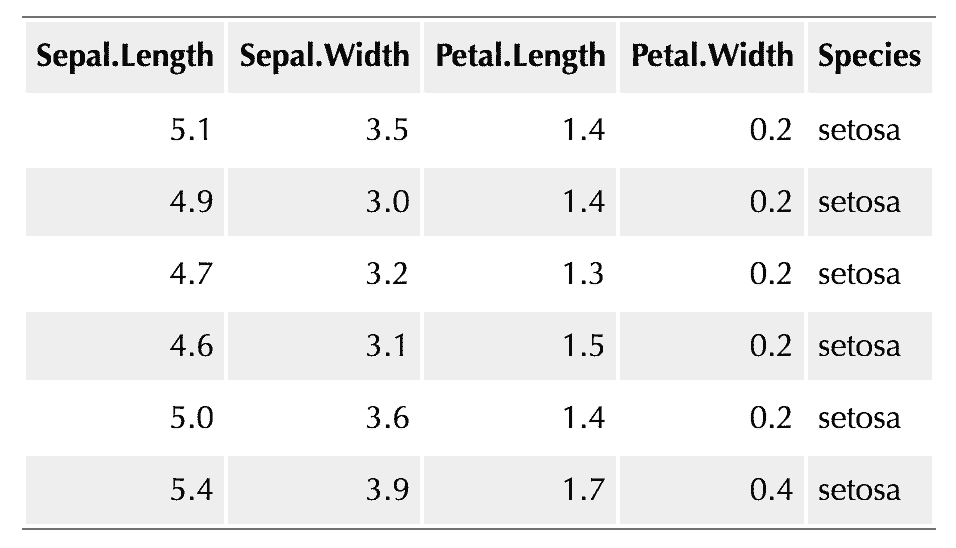
\includegraphics[width=0.7\linewidth,height=1\textheight,keepaspectratio]{JP/images/striped-table} 

}

\caption{HTML と CSS で作成したストライプ背景の表}\label{fig:striped-table}
\end{figure}

\hypertarget{kableextra}{%
\section{\texorpdfstring{\textbf{kableExtra} パッケージ}{kableExtra パッケージ}}\label{kableextra}}

\textbf{kableExtra} package \autocite{R-kableExtra}\index{R パッケージ!kableExtra}は \texttt{knitr::kable()} (\ref{kable}節参照) を使用して作成した表の基本機能を拡張するために設計されました. \texttt{knitr::kable()} はシンプルな設計なので (これは Yihui が怠け者であるという意味として読み流してください), 他のパッケージで見られるような機能の多くが決定的に失われてしまっています. そして \textbf{kableExtra} はこのギャップを完全に埋めてくれます. \textbf{kableExtra} について最も驚異することは, 表のほとんどの機能, 例えば, 図\ref{fig:striped-table}のようなストライプ背景の表をつくるなどが HTML でも PDF でも動作することです.

このパッケージはいつものように CRAN からインストールできますし, GitHub (\url{https://github.com/haozhu233/kableExtra}) から開発版をインストールすることもできます.

\begin{Shaded}
\begin{Highlighting}[numbers=left,,]
\CommentTok{\# install from CRAN}
\FunctionTok{install.packages}\NormalTok{(}\StringTok{"kableExtra"}\NormalTok{)}

\CommentTok{\# install the development version}
\NormalTok{remotes}\SpecialCharTok{::}\FunctionTok{install\_github}\NormalTok{(}\StringTok{"haozhu233/kableExtra"}\NormalTok{)}
\end{Highlighting}
\end{Shaded}

発展的なドキュメントが \url{https://haozhu233.github.io/kableExtra/} にあり, \texttt{kable()} の出力を HTML や LaTeX 出力でどうカスタマイズするかについて多くの使用例が掲載されています. 我々としてはご自分でドキュメントを読むことをおすすめし, ここでは一部の例だけを提示します.

\textbf{kableExtra} パッケージはパイプ演算子 \texttt{\%\textgreater{}\%} を前面に出しています. \texttt{kable()} の出力に \textbf{kableExtra} のスタイル関数を接続することができます. 例えばこのように.

\begin{Shaded}
\begin{Highlighting}[numbers=left,,]
\FunctionTok{library}\NormalTok{(knitr)}
\FunctionTok{library}\NormalTok{(kableExtra)}
\FunctionTok{kable}\NormalTok{(iris) }\SpecialCharTok{\%\textgreater{}\%}
  \FunctionTok{kable\_styling}\NormalTok{(}\AttributeTok{latex\_options =} \StringTok{"striped"}\NormalTok{)}
\end{Highlighting}
\end{Shaded}

\hypertarget{set-the-font-size}{%
\subsection{フォントサイズを設定する}\label{set-the-font-size}}

\textbf{kableExtra}\index{kableExtra!kable\_styling()} パッケージの \texttt{kable\_styling()} 関数によってテーブル全体のスタイルを設定できます. 例えばページ上での表のアラインメント, 幅, フォントサイズなどです. 以下は小さいフォントサイズを使う例です.

\begin{Shaded}
\begin{Highlighting}[numbers=left,,]
\FunctionTok{kable}\NormalTok{(}\FunctionTok{head}\NormalTok{(iris, }\DecValTok{5}\NormalTok{), }\AttributeTok{booktabs =} \ConstantTok{TRUE}\NormalTok{) }\SpecialCharTok{\%\textgreater{}\%}
  \FunctionTok{kable\_styling}\NormalTok{(}\AttributeTok{font\_size =} \DecValTok{8}\NormalTok{)}
\end{Highlighting}
\end{Shaded}

\begin{table}[H]
\centering\begingroup\fontsize{8}{10}\selectfont

\begin{tabular}{rrrrl}
\toprule
Sepal.Length & Sepal.Width & Petal.Length & Petal.Width & Species\\
\midrule
5.1 & 3.5 & 1.4 & 0.2 & setosa\\
4.9 & 3.0 & 1.4 & 0.2 & setosa\\
4.7 & 3.2 & 1.3 & 0.2 & setosa\\
4.6 & 3.1 & 1.5 & 0.2 & setosa\\
5.0 & 3.6 & 1.4 & 0.2 & setosa\\
\bottomrule
\end{tabular}
\endgroup{}
\end{table}

\hypertarget{style-specific-rows-columns}{%
\subsection{特定の行・列のスタイルを設定する}\label{style-specific-rows-columns}}

関数 \texttt{row\_spec()}\index{kableExtra!row\_spec()} と \texttt{column\_spec()}\index{kableExtra!column\_spec()} はそれぞれ個別の行と列のスタイル設定に使うことができます. 以下の例では第1行をボールドイタリックにし, 第2, 第3行を黒色背景と白色文字にし, 第4行にアンダーラインを引きタイプフェースを変更し, 第5行を回転させ, そして第5列に打ち消し線を引きます.

\begin{Shaded}
\begin{Highlighting}[numbers=left,,]
\FunctionTok{kable}\NormalTok{(}\FunctionTok{head}\NormalTok{(iris, }\DecValTok{5}\NormalTok{), }\AttributeTok{align =} \StringTok{\textquotesingle{}c\textquotesingle{}}\NormalTok{, }\AttributeTok{booktabs =} \ConstantTok{TRUE}\NormalTok{) }\SpecialCharTok{\%\textgreater{}\%}
  \FunctionTok{row\_spec}\NormalTok{(}\DecValTok{1}\NormalTok{, }\AttributeTok{bold =} \ConstantTok{TRUE}\NormalTok{, }\AttributeTok{italic =} \ConstantTok{TRUE}\NormalTok{) }\SpecialCharTok{\%\textgreater{}\%} 
  \FunctionTok{row\_spec}\NormalTok{(}\DecValTok{2}\SpecialCharTok{:}\DecValTok{3}\NormalTok{, }\AttributeTok{color =} \StringTok{\textquotesingle{}white\textquotesingle{}}\NormalTok{, }\AttributeTok{background =} \StringTok{\textquotesingle{}black\textquotesingle{}}\NormalTok{) }\SpecialCharTok{\%\textgreater{}\%}
  \FunctionTok{row\_spec}\NormalTok{(}\DecValTok{4}\NormalTok{, }\AttributeTok{underline =} \ConstantTok{TRUE}\NormalTok{, }\AttributeTok{monospace =} \ConstantTok{TRUE}\NormalTok{) }\SpecialCharTok{\%\textgreater{}\%} 
  \FunctionTok{row\_spec}\NormalTok{(}\DecValTok{5}\NormalTok{, }\AttributeTok{angle =} \DecValTok{45}\NormalTok{) }\SpecialCharTok{\%\textgreater{}\%} 
  \FunctionTok{column\_spec}\NormalTok{(}\DecValTok{5}\NormalTok{, }\AttributeTok{strikeout =} \ConstantTok{TRUE}\NormalTok{)}
\end{Highlighting}
\end{Shaded}

\begin{tabular}{cccc>{}c}
\toprule
Sepal.Length & Sepal.Width & Petal.Length & Petal.Width & Species\\
\midrule
\em{\textbf{5.1}} & \em{\textbf{3.5}} & \em{\textbf{1.4}} & \em{\textbf{0.2}} & \sout{\em{\textbf{setosa}}}\\
\cellcolor{black}{\textcolor{white}{4.9}} & \cellcolor{black}{\textcolor{white}{3.0}} & \cellcolor{black}{\textcolor{white}{1.4}} & \cellcolor{black}{\textcolor{white}{0.2}} & \sout{\cellcolor{black}{\textcolor{white}{setosa}}}\\
\cellcolor{black}{\textcolor{white}{4.7}} & \cellcolor{black}{\textcolor{white}{3.2}} & \cellcolor{black}{\textcolor{white}{1.3}} & \cellcolor{black}{\textcolor{white}{0.2}} & \sout{\cellcolor{black}{\textcolor{white}{setosa}}}\\
\underline{\ttfamily{4.6}} & \underline{\ttfamily{3.1}} & \underline{\ttfamily{1.5}} & \underline{\ttfamily{0.2}} & \sout{\underline{\ttfamily{setosa}}}\\
\rotatebox{45}{5.0} & \rotatebox{45}{3.6} & \rotatebox{45}{1.4} & \rotatebox{45}{0.2} & \sout{\rotatebox{45}{setosa}}\\
\bottomrule
\end{tabular}

同様に, \texttt{cell\_spec()}\index{kableExtra!cell\_spec()} 関数で個別のセルにスタイル設定できます.

\hypertarget{group-rows-columns}{%
\subsection{行・列をグループ化する}\label{group-rows-columns}}

行や列をそれぞれ, \texttt{pack\_rows()}\index{kableExtra!pack\_rows()} と \texttt{add\_header\_above()}\index{kableExtra!add\_header\_above()} 関数でまとめることができます. \texttt{collapse\_rows()}\index{kableExtra!collapse\_rows()} 関数で行を崩し, セルを複数行にまたがらせることができます. 以下は行をグループ化したカスタムテーブルヘッダの例です.

\begin{Shaded}
\begin{Highlighting}[numbers=left,,]
\NormalTok{iris2 }\OtherTok{\textless{}{-}}\NormalTok{ iris[}\DecValTok{1}\SpecialCharTok{:}\DecValTok{5}\NormalTok{, }\FunctionTok{c}\NormalTok{(}\DecValTok{1}\NormalTok{, }\DecValTok{3}\NormalTok{, }\DecValTok{2}\NormalTok{, }\DecValTok{4}\NormalTok{, }\DecValTok{5}\NormalTok{)]}
\FunctionTok{names}\NormalTok{(iris2) }\OtherTok{\textless{}{-}} \FunctionTok{gsub}\NormalTok{(}\StringTok{\textquotesingle{}[.].+\textquotesingle{}}\NormalTok{, }\StringTok{\textquotesingle{}\textquotesingle{}}\NormalTok{, }\FunctionTok{names}\NormalTok{(iris2))}
\FunctionTok{kable}\NormalTok{(iris2, }\AttributeTok{booktabs =} \ConstantTok{TRUE}\NormalTok{) }\SpecialCharTok{\%\textgreater{}\%}
  \FunctionTok{add\_header\_above}\NormalTok{(}\FunctionTok{c}\NormalTok{(}\StringTok{"長さ"} \OtherTok{=} \DecValTok{2}\NormalTok{, }\StringTok{"幅"} \OtherTok{=} \DecValTok{2}\NormalTok{, }\StringTok{" "} \OtherTok{=} \DecValTok{1}\NormalTok{)) }\SpecialCharTok{\%\textgreater{}\%} 
  \FunctionTok{add\_header\_above}\NormalTok{(}\FunctionTok{c}\NormalTok{(}\StringTok{"Measurements"} \OtherTok{=} \DecValTok{4}\NormalTok{, }\StringTok{"More attributes"} \OtherTok{=} \DecValTok{1}\NormalTok{))}
\end{Highlighting}
\end{Shaded}

\begin{tabular}{rrrrl}
\toprule
\multicolumn{4}{c}{Measurements} & \multicolumn{1}{c}{More attributes} \\
\cmidrule(l{3pt}r{3pt}){1-4} \cmidrule(l{3pt}r{3pt}){5-5}
\multicolumn{2}{c}{長さ} & \multicolumn{2}{c}{幅} & \multicolumn{1}{c}{ } \\
\cmidrule(l{3pt}r{3pt}){1-2} \cmidrule(l{3pt}r{3pt}){3-4}
Sepal & Petal & Sepal & Petal & Species\\
\midrule
5.1 & 1.4 & 3.5 & 0.2 & setosa\\
4.9 & 1.4 & 3.0 & 0.2 & setosa\\
4.7 & 1.3 & 3.2 & 0.2 & setosa\\
4.6 & 1.5 & 3.1 & 0.2 & setosa\\
5.0 & 1.4 & 3.6 & 0.2 & setosa\\
\bottomrule
\end{tabular}

\texttt{add\_header\_above()} 内の名前付きベクトルに対して, 名前がテーブルヘッダにテキストとして表示され, 整数値のベクトルが対応する名前の列の長さを表します. 例えば \texttt{"Length" = 2} が \texttt{Length} が2列にまたがることを意味します.

以下は \texttt{pack\_rows()} の例です. \texttt{index} 引数の意味は既に説明した \texttt{add\_header\_above()} の引数と似ています.

\begin{Shaded}
\begin{Highlighting}[numbers=left,,]
\NormalTok{iris3 }\OtherTok{\textless{}{-}}\NormalTok{ iris[}\FunctionTok{c}\NormalTok{(}\DecValTok{1}\SpecialCharTok{:}\DecValTok{2}\NormalTok{, }\DecValTok{51}\SpecialCharTok{:}\DecValTok{54}\NormalTok{, }\DecValTok{101}\SpecialCharTok{:}\DecValTok{103}\NormalTok{), ]}
\FunctionTok{kable}\NormalTok{(iris3[, }\DecValTok{1}\SpecialCharTok{:}\DecValTok{4}\NormalTok{], }\AttributeTok{booktabs =} \ConstantTok{TRUE}\NormalTok{) }\SpecialCharTok{\%\textgreater{}\%} \FunctionTok{pack\_rows}\NormalTok{(}
  \AttributeTok{index =} \FunctionTok{c}\NormalTok{(}\StringTok{"setosa"} \OtherTok{=} \DecValTok{2}\NormalTok{, }\StringTok{"versicolor"} \OtherTok{=} \DecValTok{4}\NormalTok{, }\StringTok{"virginica"} \OtherTok{=} \DecValTok{3}\NormalTok{)}
\NormalTok{)}
\end{Highlighting}
\end{Shaded}

\begin{tabular}{lrrrr}
\toprule
  & Sepal.Length & Sepal.Width & Petal.Length & Petal.Width\\
\midrule
\addlinespace[0.3em]
\multicolumn{5}{l}{\textbf{setosa}}\\
\hspace{1em}1 & 5.1 & 3.5 & 1.4 & 0.2\\
\hspace{1em}2 & 4.9 & 3.0 & 1.4 & 0.2\\
\addlinespace[0.3em]
\multicolumn{5}{l}{\textbf{versicolor}}\\
\hspace{1em}51 & 7.0 & 3.2 & 4.7 & 1.4\\
\hspace{1em}52 & 6.4 & 3.2 & 4.5 & 1.5\\
\hspace{1em}53 & 6.9 & 3.1 & 4.9 & 1.5\\
\hspace{1em}54 & 5.5 & 2.3 & 4.0 & 1.3\\
\addlinespace[0.3em]
\multicolumn{5}{l}{\textbf{virginica}}\\
\hspace{1em}101 & 6.3 & 3.3 & 6.0 & 2.5\\
\hspace{1em}102 & 5.8 & 2.7 & 5.1 & 1.9\\
\hspace{1em}103 & 7.1 & 3.0 & 5.9 & 2.1\\
\bottomrule
\end{tabular}

\hypertarget{scaling-down-wide-tables-in-latex}{%
\subsection{LaTeX で表を縮小する}\label{scaling-down-wide-tables-in-latex}}

HTML や LaTeX 出力特有の機能もいくつかあります. 例えば横向きページは LaTeX でのみ意味をなすので, \textbf{kableExtra} の \texttt{landscape()} 関数\index{kableExtra!landscape()}は LaTeX でのみ機能します. 以下はページに合わせて表を縮小する例です. 縮小しなければ横に長すぎる表になります.

\begin{Shaded}
\begin{Highlighting}[numbers=left,,]
\NormalTok{tab }\OtherTok{\textless{}{-}} \FunctionTok{kable}\NormalTok{(}\FunctionTok{tail}\NormalTok{(mtcars, }\DecValTok{5}\NormalTok{), }\AttributeTok{booktabs =} \ConstantTok{TRUE}\NormalTok{)}
\NormalTok{tab  }\CommentTok{\# 長すぎる元の表}
\end{Highlighting}
\end{Shaded}

\begin{tabular}{lrrrrrrrrrrr}
\toprule
  & mpg & cyl & disp & hp & drat & wt & qsec & vs & am & gear & carb\\
\midrule
Lotus Europa & 30.4 & 4 & 95.1 & 113 & 3.77 & 1.513 & 16.9 & 1 & 1 & 5 & 2\\
Ford Pantera L & 15.8 & 8 & 351.0 & 264 & 4.22 & 3.170 & 14.5 & 0 & 1 & 5 & 4\\
Ferrari Dino & 19.7 & 6 & 145.0 & 175 & 3.62 & 2.770 & 15.5 & 0 & 1 & 5 & 6\\
Maserati Bora & 15.0 & 8 & 301.0 & 335 & 3.54 & 3.570 & 14.6 & 0 & 1 & 5 & 8\\
Volvo 142E & 21.4 & 4 & 121.0 & 109 & 4.11 & 2.780 & 18.6 & 1 & 1 & 4 & 2\\
\bottomrule
\end{tabular}

\begin{Shaded}
\begin{Highlighting}[numbers=left,,]
\NormalTok{tab }\SpecialCharTok{\%\textgreater{}\%}
  \FunctionTok{kable\_styling}\NormalTok{(}\AttributeTok{latex\_options =} \StringTok{"scale\_down"}\NormalTok{)}
\end{Highlighting}
\end{Shaded}

\begin{table}[H]
\centering
\resizebox{\linewidth}{!}{
\begin{tabular}{lrrrrrrrrrrr}
\toprule
  & mpg & cyl & disp & hp & drat & wt & qsec & vs & am & gear & carb\\
\midrule
Lotus Europa & 30.4 & 4 & 95.1 & 113 & 3.77 & 1.513 & 16.9 & 1 & 1 & 5 & 2\\
Ford Pantera L & 15.8 & 8 & 351.0 & 264 & 4.22 & 3.170 & 14.5 & 0 & 1 & 5 & 4\\
Ferrari Dino & 19.7 & 6 & 145.0 & 175 & 3.62 & 2.770 & 15.5 & 0 & 1 & 5 & 6\\
Maserati Bora & 15.0 & 8 & 301.0 & 335 & 3.54 & 3.570 & 14.6 & 0 & 1 & 5 & 8\\
Volvo 142E & 21.4 & 4 & 121.0 & 109 & 4.11 & 2.780 & 18.6 & 1 & 1 & 4 & 2\\
\bottomrule
\end{tabular}}
\end{table}

HTML 版をご覧なら, 上の2つの表に違いが見られないでしょう.

\hypertarget{table-other}{%
\section{その他の表作成パッケージ}\label{table-other}}

多くの作表用 R パッケージがあります\index{R パッケージ!作表パッケージ}. \texttt{kable()} (\ref{kable}節) と\textbf{kableExtra} (\ref{kableextra}節) を紹介した)主な理由は他のパッケージより良いからではなく, 私がこれらにのみ詳しかったからです.\footnote{平たく言うと, 自分では表を全く使いませんから, 洗練された表を作る方法を学ぶ強いモチベーションがありませんでした.} 存在は知っていますがあまり詳しくないパッケージを次に列挙します.\footnote{\textbf{訳注}: これらの差異について, 翻訳者も自信の作成したドキュメントでいくらか言及しています \url{https://gedevan-aleksizde.github.io/rmdja/advanced-tabulate.html}} ご自分で確認し, 目的に最も合っているものを決めることができます.

\begin{itemize}
\item
  \textbf{flextable} \autocite{R-flextable} と \textbf{huxtable} \autocite{R-huxtable}: 幅広い種類の出力フォーマットをサポートするパッケージを探しているなら, \textbf{flextable} と \textbf{huxtable} が最善の2つの選択です. HTML, LaTeX. そして Office フォーマットを全てサポートし, よく使われる表の機能 (例えば条件付き書式とか) のほとんどをサポートしています. \textbf{flextable} の詳細は \url{https://davidgohel.github.io/flextable/} で, \textbf{huxtable} のドキュメントは \url{https://hughjonesd.github.io/huxtable/} で見られます.
\item
  \textbf{gt} \autocite{R-gt}: 表のヘッダ, (題名・副題), 列のラベル, 表の本体, 行グループのラベル, 表のフッタといった異なる表のパーツをまとめて表を構成することができます. 数字のフォーマットを指定したり, セルの背景色に影をつけたりもできます. 現在は \textbf{gt} は主に HTML 出力をサポートしています.\footnote{LaTeX や Word といった他の出力フォーマットへのサポートが必要ならば, \textbf{gtsummary} パッケージ \autocite{R-gtsummary} はとても有望な \textbf{gt} を下地に拡張しています. \url{https://github.com/ddsjoberg/gtsummary}} 詳細は \url{https://gt.rstudio.com} で見られます.
\item
  \textbf{formattable} \autocite{R-formattable}: \texttt{percent()}, \texttt{accounting()} といった数値を整形するものや, テキストの書式, 背景色やカラーバー, アイコンの追加などで数値を強調するなど, 表の列のスタイルを設定する関数を提供してくれます. \textbf{gt} のように, このパッケージも主に HTML フォーマットをサポートしています. 詳細は GitHub プロジェクトの \url{https://github.com/renkun-ken/formattable} で見ることができます.
\item
  \textbf{DT} \autocite{R-DT}: 作者なのでこのパッケージには精通していると思っていますが, HTML フォーマットのみサポートしているため, 独立した節を設けて紹介したりはしません. \textbf{DT} は JavaScript ライブラリの \textbf{DataTables} を下地に構築されたもので, HTML ページ上で静的な表をインタラクティブな表に変えることができます. 表をソートしたり, 検索したり, ページ移動したりできるでしょう. \textbf{DT} はセルの整形もサポートしており, インタラクティブなアプリケーションの構築のため Shiny と連携して動作し, 多くの \textbf{DaataTables} の拡張を導入します. 例えばエクセルへのエクスポート, 列の並び替えなどです. 詳細はパッケージのリポジトリ \url{https://github.com/rstudio/DT} を見てください.
\item
  \textbf{reactable} \autocite{R-reactable}: \textbf{DT} と同様にこのパッケージは JavaScript ライブラリを元にしてインタラクティブな表を作成します. 平たく言うと, 私が見る限り, 行のグループ化や HTML ウィジェットの埋め込み機能などいくつかの観点で \textbf{DT} より優れているようです. もし \textbf{reactable} が 2015年時点で存在していれば, 私は \textbf{DT} を開発していなかったと思います. よってあなたはこのパッケージのドキュメント \url{https://glin.github.io/reactable/} を読み, どちらが目的に合ったものかを知ることもできるでしょう.
\item
  \textbf{rhandsontable} \autocite{R-rhandsontable}: これも \textbf{DT} と似ており, そして表上でデータを直接編集できるなど Excel っぽさがあります. 詳しく学ぶには \url{https://jrowen.github.io/rhandsontable/} を見てください.
\item
  \textbf{pixiedust} \autocite{R-pixiedust}: \textbf{broom} パッケージ \autocite{R-broom} を介して統計モデル (線形モデルとか) 向けの表を作るのが特徴です. Markdown, HTML, LaTeX 出力フォーマットをサポートしています. リポジトリは \url{https://github.com/nutterb/pixiedust} です.
\item
  \textbf{stargazer} \autocite{R-stargazer}: 回帰モデルと要約統計量の表を整形するのが特徴です. このパッケージは CRAN の \url{https://cran.r-project.org/package=stargazer} にあります.
\item
  \textbf{xtable} \autocite{R-xtable}: おそらく最古の作表パッケージです. 最初のリリースは2000年になります. LaTeX と HTML フォーマットの両方をサポートしています. パッケージは CRAN の \url{https://cran.r-project.org/package=xtable} にあります.
\end{itemize}

その他のパッケージは紹介しませんが, 名前だけ挙げておきます. \textbf{tables} \autocite{R-tables}, \textbf{pander} \autocite{R-pander}, \textbf{tangram} \autocite{R-tangram}, \textbf{ztable} \autocite{R-ztable}, \textbf{condformat} \autocite{R-condformat} があります.

\hypertarget{chunk-options}{%
\chapter{チャンクオプション}\label{chunk-options}}

図\ref{fig:rmdworkflow}が表すように, \textbf{knitr} パッケージは R Markdown においてきわめて重要な役割を持ちます. この章と次の3つの章では \textbf{knitr} に関連するレシピをお見せします.

R のチャンクを処理する際には, \textbf{knitr} の挙動を微調整するのに 50 のチャンクオプション (chunk options) \index{チャンクオプション}\index{chunk option|see{チャンクオプション}}が使われる可能性があります. 完全なリストは \url{https://yihui.org/knitr/options/} のオンラインドキュメントをご覧ください.\footnote{\textbf{訳注}: 翻訳者に寄る日本語訳はこちら: \url{https://gedevan-aleksizde.github.io/knitr-doc-ja/options.html}} 利便性のため, 本書の 付録\ref{full-options}としてこのドキュメントのコピーを掲載しました.

続く各節では, チャンクオプションを個別のコードチャンクに適用する例のみを示します. ただし, どのチャンクオプションもグローバル設定で文書全体に適用できるので, コードチャンク1つ1つに繰り返しオプションを書かなくても良いという事実を覚えてください. グローバルにチャンクオプションを設定するには, いずれかのコードチャンクで \texttt{knitr::opts\_chunk\$set()}\index{チャンクオプション!グローバルに設定する} を呼び出してください. たいていは文書の中で最初のチャンクオプションです. 例えばこのように.

\begin{Shaded}
\begin{Highlighting}[]
\InformationTok{\textasciigrave{}\textasciigrave{}\textasciigrave{}\{r, include=FALSE\}}
\InformationTok{knitr::opts\_chunk$set(}
\InformationTok{  comment = "\#\textgreater{}", echo = FALSE, fig.width = 6}
\InformationTok{)}
\InformationTok{\textasciigrave{}\textasciigrave{}\textasciigrave{}}
\end{Highlighting}
\end{Shaded}

\hypertarget{chunk-variable}{%
\section{チャンクオプションに変数を使う}\label{chunk-variable}}

大抵の場合, 例えば \texttt{fig.width = 6} のようにチャンクオプションは定数をとりますが, 簡単であるか複雑であるかに関わらず, 任意の R コードを与えることもできます. 単純なケースはチャンクオプションに通せる変数\index{チャンクオプション!変数の値}です. 変数もまた R コードであることに注意してください. 例えば文書の冒頭で変数として図の幅を定義して, その後の他のコードチャンクで使うことができるので, それ以降の幅を簡単に変更できます.

\begin{Shaded}
\begin{Highlighting}[]
\InformationTok{\textasciigrave{}\textasciigrave{}\textasciigrave{}\{r\}}
\InformationTok{my\_width \textless{}{-} 7}
\InformationTok{\textasciigrave{}\textasciigrave{}\textasciigrave{}}

\InformationTok{\textasciigrave{}\textasciigrave{}\textasciigrave{}\{r, fig.width=my\_width\}}
\InformationTok{plot(cars)}
\InformationTok{\textasciigrave{}\textasciigrave{}\textasciigrave{}}
\end{Highlighting}
\end{Shaded}

以下はチャンクオプショで \texttt{if-else} 文を使う例です\index{チャンクオプション!if else ロジック}.

\begin{Shaded}
\begin{Highlighting}[]
\InformationTok{\textasciigrave{}\textasciigrave{}\textasciigrave{}\{r\}}
\InformationTok{fig\_small \textless{}{-} FALSE  \# 大きい図に対しては TRUE に変更}
\InformationTok{width\_small \textless{}{-} 4}
\InformationTok{width\_large \textless{}{-} 8}
\InformationTok{\textasciigrave{}\textasciigrave{}\textasciigrave{}}

\InformationTok{\textasciigrave{}\textasciigrave{}\textasciigrave{}\{r, fig.width=if (fig\_small) width\_small else width\_large\}}
\InformationTok{plot(cars)}
\InformationTok{\textasciigrave{}\textasciigrave{}\textasciigrave{}}
\end{Highlighting}
\end{Shaded}

さらに以下にもう1つの例として, 必要なパッケージが使用可能な場合のみコードチャンクを評価する (つまり実行する) ものを示します.

\begin{Shaded}
\begin{Highlighting}[]
\InformationTok{\textasciigrave{}\textasciigrave{}\textasciigrave{}\{r, eval=require(\textquotesingle{}leaflet\textquotesingle{})\}}
\InformationTok{library(leaflet)}
\InformationTok{leaflet() \%\textgreater{}\% addTiles()}
\InformationTok{\textasciigrave{}\textasciigrave{}\textasciigrave{}}
\end{Highlighting}
\end{Shaded}

意図が分からない方のために説明しますと, \texttt{require(\textquotesingle{}package\textquotesingle{})} はパッケージが使用可能なら \texttt{TRUE} を返し, そうでないなら \texttt{FALSE} を返します.

\hypertarget{opts-error}{%
\section{エラーが起こっても中止しない}\label{opts-error}}

時として, 例えば R のチュートリアルのために, わざとエラーを見せたいこともあるかもしれません. デフォルトでは, Rmd 文書のコードチャンクでのエラーは R の処理を停止させます. R の処理を停めることなくエラーを見せたいなら, 例えばこのように \texttt{error = TRUE}\index{チャンクオプション!error} チャンクオプションを使うこともできます.

\begin{Shaded}
\begin{Highlighting}[]
\InformationTok{\textasciigrave{}\textasciigrave{}\textasciigrave{}\{r, error=TRUE\}}
\InformationTok{1 + "a"}
\InformationTok{\textasciigrave{}\textasciigrave{}\textasciigrave{}}
\end{Highlighting}
\end{Shaded}

Rmd 文書をコンパイルすると, 出力文書上でのエラーメッセージはこのような見た目になります.

\begin{verbatim}
Error in 1 + "a":  二項演算子の引数が数値ではありません 
\end{verbatim}

R Markdown では \texttt{error = FALSE} がデフォルトであり, これはコードチャンクの実行時のエラーは処理を停止させます.

\hypertarget{dev-vector}{%
\section{同じグラフを複数の出力フォーマットに}\label{dev-vector}}

ほとんどの場合, 1つの図に対して \texttt{png} や \texttt{pdf} といった1つの画像フォーマットにしたいでしょう. 画像フォーマットはチャンクオプション \texttt{dev}\index{チャンクオプション!dev}\index{図!グラフィックデバイス} で操作できます. つまり, グラフをレンダリングするグラフィックデバイスを意味します. このオプションはデバイス名のベクトルをとることができます. これが例です.

\begin{Shaded}
\begin{Highlighting}[]
\InformationTok{\textasciigrave{}\textasciigrave{}\textasciigrave{}\{r, dev=c(\textquotesingle{}png\textquotesingle{}, \textquotesingle{}pdf\textquotesingle{}, \textquotesingle{}svg\textquotesingle{}, \textquotesingle{}tiff\textquotesingle{})\}}
\InformationTok{plot(cars)}
\InformationTok{\textasciigrave{}\textasciigrave{}\textasciigrave{}}
\end{Highlighting}
\end{Shaded}

出力文書には最初のフォーマットのみが使われますが, 残りのフォーマットに対応する画像も生成されます. 例えば, レポートでは \texttt{png} 画像を掲載するが, 同じ画像の \texttt{tiff} 形式が求められるというように, 追加で異なるフォーマットの図の提出が要求されるような場合に便利でしょう.

デフォルトでは, 典型として画像ファイルは出力文書がレンダリングされた後に削除されます. ファイルを保持する方法は\ref{keep-files}節を参照してください.

\hypertarget{cache}{%
\section{時間のかかるチャンクをキャッシュする}\label{cache}}

コードチャンクの実行に時間がかかる場合, チャンクオプション \texttt{cache = TRUE}\index{チャンクオプション!cache}\index{キャッシュ} で結果をキャッシュすることを検討するとよいでしょう. キャッシュが有効な場合, このコードが以前にも実行され, その後コードに変更がないならば, \textbf{knitr} はこの実行を飛ばします. コードチャンクを変更し, つまりコードまたはチャンクオプションを修正したなら, 過去のキャッシュは自動的に無効になり \textbf{knitr} はもう一度チャンクをキャッシュします.

キャッシュされたコードチャンクに関しては, チャンクが再度実行されたかのように, 過去の実行結果から出力とオブジェクトが自動的に読み込まれます. キャッシュを取ることは結果を計算するより読み込んだほうがはるかに速いという場合に役に立ちます. しかしながら, うまい話というのは世に存在しません. あなたの使う場面にもよりますが, キャッシュがどのように動作するかをより学びぶ必要があるかもしれません, 特に \href{https://yihui.org/en/2018/06/cache-invalidation/}{cache invalidation} を. これにより, \textbf{knitr}がしょっちゅうキャッシュを無効化したり, あるいは時に無効化が十分できていない理由に混乱することなく, あなたはキャッシュの利点を最大限活かすことができます.

最も適切なキャッシュの使用例は, コードチャンク内での計算に非常に時間がかかるり, そして \texttt{options()} を使って R のグローバルオプションを変更するといった副産物 (このような変更はキャッシュされません) の一切ない R オブジェクトの保存と再読込に使うことです. コードチャンクに副産物があるなら, キャッシュを使わないことをお薦めします.

最初のほうで簡単に書いたように, キャッシュはチャンクオプションに依存します. もし \texttt{include} 以外のチャンクオプションを変更したら, キャッシュは無効化されます. この性質はよくある問題を解決するのに使うことができます. それは外部データファイルを読み込むときに, ファイルが更新されていたならキャッシュを無効化したい, というような場合です. 単純に \texttt{cache = TRUE} を使うだけでは不十分です.

\begin{Shaded}
\begin{Highlighting}[]
\InformationTok{\textasciigrave{}\textasciigrave{}\textasciigrave{}\{r import{-}data, cache=TRUE\}}
\InformationTok{d \textless{}{-} read.csv(\textquotesingle{}my{-}precious.csv\textquotesingle{})}
\InformationTok{\textasciigrave{}\textasciigrave{}\textasciigrave{}}
\end{Highlighting}
\end{Shaded}

\textbf{knitr} にデータファイルが変更されたかどうかを教えなければなりません. 1つの方法として別のチャンクオプション \texttt{cache.extra = file.mtime(\textquotesingle{}my-precious.csv\textquotesingle{})}\index{チャンクオプション!cache.extra} を, あるいはより厳密に \texttt{cache.extra = tools::md5sum(\textquotesingle{}my-precious.csv\textquotesingle{})} を追加することがあります. 前者はファイルの更新時刻が変更されたらキャッシュを無効化する, という意味です. 後者はファイルの中身が変更されたらキャッシュを更新するということです. \texttt{cache.extra} は \textbf{knitr} の組み込みのチャンクオプションではないということに注意してください. 他の組み込みのオプション名と競合しない限り, この用途のオプションには好きな名前を使うことができます.

同様に, 他の情報をキャッシュと関連付けることができます. 例えば R のバージョンなら \texttt{cache.extra = getRversion()}, 日付なら \texttt{cache.extra = Sys.Date()}, オペレーティングシステムなら \texttt{cache.extra = Sys.info(){[}{[}\textquotesingle{}sysname\textquotesingle{}{]}{]}} というようにすると, これらの条件が変更されたときにキャッシュは正しく無効化されます.

文書全体で \texttt{cache = TRUE} を設定することはお薦めしません. キャッシュはかなり扱いにくいものです. そうではなく, 実行に時間がかかり副産物のないとはっきりしているコードチャンクに対してのみ個別にキャッシュを有効化することをお薦めします.

\textbf{knitr} のキャッシュの設計に不満があるなら, 自分でオブジェクトのキャッシュを取ることもできます. 以下はごく簡単な例です.

\begin{Shaded}
\begin{Highlighting}[numbers=left,,]
\ControlFlowTok{if}\NormalTok{ (}\FunctionTok{file.exists}\NormalTok{(}\StringTok{"results.rds"}\NormalTok{)) \{}
\NormalTok{  res }\OtherTok{\textless{}{-}} \FunctionTok{readRDS}\NormalTok{(}\StringTok{"results.rds"}\NormalTok{)}
\NormalTok{\} }\ControlFlowTok{else}\NormalTok{ \{}
\NormalTok{  res }\OtherTok{\textless{}{-}} \FunctionTok{compute\_it}\NormalTok{()  }\CommentTok{\# a time{-}consuming function}
  \FunctionTok{saveRDS}\NormalTok{(res, }\StringTok{"results.rds"}\NormalTok{)}
\NormalTok{\}}
\end{Highlighting}
\end{Shaded}

この例では, キャッシュを無効化する唯一の, そして簡単な方法は \texttt{result.rds\textasciigrave{}\textasciigrave{}\ ファイルを削除することです.\ この簡単なキャッシュのしくみが気に入ったなら,\ \textbackslash{}@ref(cache-rds)節で紹介する}xfun::cache\_rds()`\index{xfun!cache\_rds()} を使うこともできます.

\hypertarget{cache-path}{%
\section{複数の出力フォーマットに対してチャンクをキャッシュする}\label{cache-path}}

\texttt{cache = TRUE}\index{チャンクオプション!cache}\index{キャッシュ} でキャッシュが有効化されたとき, \textbf{knitr} は R コードチャンクで生成された R オブジェクトをキャッシュデータベースに書き込みます. これで次回から再読込ができます. キャッシュデータベースのパスはチャンクオプション \texttt{cache.path}\index{チャンクオプション!cache.path} によって決まります. デフォルトでは R Markdown は出力フォーマットごとに異なるキャッシュのパスを使用するので, 時間のかかるコードチャンクは出力フォーマットごとに丸ごと実行されることになります. これは不便かもしれませんが, これがデフォルトの挙動であることには理由があります. コードチャンクの出力は, 出力フォーマットに依存します. 例えばグラフを生成した時, 出力フォーマットが \texttt{word\_document} なら \texttt{!{[}text{]}(path/to/image.png)} のような Markdown 構文で図を掲載できますし, 出力フォーマットが \texttt{html\_document} なら \texttt{\textless{}img\ src="path/to/image.png"\ /\textgreater{}} が使えます.

コードチャンクにグラフなど副作用が一切ないとき, 全ての出力フォーマットで同じキャッシュデータベースを使っても安全であり, 時間を節約できます. 例えば大きなデータオブジェクトを読み込むか時間のかかるモデルを実行するかというときは, 結果は出力フォーマットに依存しませんので, 同じキャッシュデータベースを使うことができます. コードチャンクに \texttt{cache.path} を指定することでデータベースのパスを指定できます. これが例です.

\begin{Shaded}
\begin{Highlighting}[]
\InformationTok{\textasciigrave{}\textasciigrave{}\textasciigrave{}\{r important{-}computing, cache=TRUE, cache.path="cache/"\}}
\InformationTok{\textasciigrave{}\textasciigrave{}\textasciigrave{}}
\end{Highlighting}
\end{Shaded}

R Markdown ではデフォルトでは \texttt{cache.path = "INPUT\_cache/FORMAT/"} で, \texttt{INPUT} には入力ファイル名が, \texttt{FORMAT} には \texttt{html}, \texttt{latex}, \texttt{docx} といった出力フォーマット名が入ります.

\hypertarget{cache-lazy}{%
\section{巨大オブジェクトをキャッシュする}\label{cache-lazy}}

チャンクオプション \texttt{cache = TRUE} を使うと, キャッシュされたオブジェクトは R セッション内で遅延読み込みされます. これはオブジェクトが実際にコード内で使用されるまで\index{caching}キャッシュデータベースから読み込まれないことを意味します. 以降の文書内で全てのオブジェクトが使われるわけではない場合にメモリを多少節約することができます. 例えば大きなデータオブジェクトを読み込んだが, 以降の分析ではその一部しか使わないなら, 元のデータオブジェクトはキャッシュデータベースから読み込まれません.

\begin{Shaded}
\begin{Highlighting}[]
\InformationTok{\textasciigrave{}\textasciigrave{}\textasciigrave{}\{r, read{-}data, cache=TRUE\}}
\InformationTok{full \textless{}{-} read.csv("HUGE.csv")}
\InformationTok{rows \textless{}{-} subset(full, price \textgreater{} 100)}
\InformationTok{\# next we only use \textasciigrave{}rows\textasciigrave{}}
\InformationTok{\textasciigrave{}\textasciigrave{}\textasciigrave{}}

\InformationTok{\textasciigrave{}\textasciigrave{}\textasciigrave{}\{r\}}
\InformationTok{plot(rows)}
\InformationTok{\textasciigrave{}\textasciigrave{}\textasciigrave{}}
\end{Highlighting}
\end{Shaded}

しかし, オブジェクトが大きすぎるときは, このようなエラーに遭遇するかもしれません.

\begin{Shaded}
\begin{Highlighting}[]
\NormalTok{Error }\ControlFlowTok{in} \FunctionTok{lazyLoadDBinsertVariable}\NormalTok{(vars[i], ... }
\NormalTok{  long vectors not supported yet}\SpecialCharTok{:}\NormalTok{ ...}
\NormalTok{Execution halted}
\end{Highlighting}
\end{Shaded}

この問題が発生したら, チャンクオプション \texttt{cache.lazy = FALSE}\index{チャンクオプション!cache.lazy} で遅延読み込みを無効にできます. チャンク内の全てのオブジェクトが即座にメモリに読み込まれます.

\hypertarget{hide-one}{%
\section{コード, テキスト出力, メッセージ, グラフを隠す}\label{hide-one}}

デフォルトでは, \textbf{knitr} はコードチャンクから, ソースコード・テキスト出力・メッセージ・警告・エラー・グラフといった可能な全ての出力を表示します. これらに対応するコードチャンクを使い, 個別に隠すことができます.

\begin{Shaded}
\begin{Highlighting}[]
\NormalTok{ソースコードを隠す.}

\InformationTok{\textasciigrave{}\textasciigrave{}\textasciigrave{}\{r, echo=FALSE\}}
\InformationTok{1 + 1}
\InformationTok{\textasciigrave{}\textasciigrave{}\textasciigrave{}}

\NormalTok{テキスト出力を隠す. }\InformationTok{\textasciigrave{}results = FALSE\textasciigrave{}}\NormalTok{ を使うのも可.}

\InformationTok{\textasciigrave{}\textasciigrave{}\textasciigrave{}\{r, results=\textquotesingle{}hide\textquotesingle{}\}}
\InformationTok{print("テキスト出力はあなたには見えない.")}
\InformationTok{\textasciigrave{}\textasciigrave{}\textasciigrave{}}

\NormalTok{メッセージを隠す.}

\InformationTok{\textasciigrave{}\textasciigrave{}\textasciigrave{}\{r, message=FALSE\}}
\InformationTok{message("このメッセージはあなたには見えない.")}
\InformationTok{\textasciigrave{}\textasciigrave{}\textasciigrave{}}

\NormalTok{警告メッセージを隠す.}

\InformationTok{\textasciigrave{}\textasciigrave{}\textasciigrave{}\{r, warning=FALSE\}}
\InformationTok{\# 警告を発生させるが抑制される}
\InformationTok{1:2 + 1:3}
\InformationTok{\textasciigrave{}\textasciigrave{}\textasciigrave{}}

\NormalTok{グラフを隠す.}

\InformationTok{\textasciigrave{}\textasciigrave{}\textasciigrave{}\{r, fig.show=\textquotesingle{}hide\textquotesingle{}\}}
\InformationTok{plot(cars)}
\InformationTok{\textasciigrave{}\textasciigrave{}\textasciigrave{}}

\NormalTok{上記のチャンクではグラフが生成されることに注意してください. 出力に表示しなくするだけです.}
\end{Highlighting}
\end{Shaded}

\textbf{knitr} に関するよくある質問の1つは, パッケージ読み込み時のメッセージを隠す方法です. 例えば \texttt{library(tidyverse)} や \texttt{library(ggplot2)} を使ったとき, いくつかの読み込みメッセージが現れます. このようなメッセージはチャンクオプション \texttt{message = FALSE} で抑制することもできます.

インデックスによってこれらの要素を表示したり隠したり選択することも出来ます. 以下の例では, ソースコードの4つ目と5つ目の式を表示し, 最初の2つのメッセージと2つ目と3つ目の警告を隠しています. コメントも式1つとして数えられることに注意してください.

\begin{Shaded}
\begin{Highlighting}[]
\InformationTok{\textasciigrave{}\textasciigrave{}\textasciigrave{}\{r, echo=c(4, 5), message=c(1, 2), warning=2:3\}}
\InformationTok{\# 乱数 N(0, 1) を生成する方法の1つ}
\InformationTok{x \textless{}{-} qnorm(runif(10))}
\InformationTok{\# だが rnorm() を使うほうが実用的}
\InformationTok{x \textless{}{-} rnorm(10)}
\InformationTok{x}

\InformationTok{for (i in 1:5) message(\textquotesingle{}ここにメッセージ \textquotesingle{}, i)}

\InformationTok{for (i in 1:5) warning(\textquotesingle{}ここにメッセージ \textquotesingle{}, i)}
\InformationTok{\textasciigrave{}\textasciigrave{}\textasciigrave{}}
\end{Highlighting}
\end{Shaded}

負のインデックスを使用することもできます. 例えば \texttt{echo = -2}\index{チャンクオプション!echo} は出力部のソースコードの2つ目の式を排除します.

同様に, \texttt{fig.keep} オプション\index{チャンクオプション!fig.keep}に対してインデックスを使うことでどのグラフを表示あるいは隠すかを選ぶこともできます. 例えば \texttt{fig.keep = 1:2} は最初の2つのグラフを残すことを意味します. このオプションにはいくつかのショートカットがあります. \texttt{fig.keep = "first"} は最初のグラフのみを残し, \texttt{fig.keep = "last"} は最後のグラフのみを残し, \texttt{fig.keep = "none"} は全てのグラフを破棄します. 2つのオプション \texttt{fig.keep = "none"} と \texttt{fig.show = "hide"} は異なることに注意してください. 前者はそもそも画像ファイルを生成しませんが, 後者はグラフを生成し隠すだけです.

\texttt{html\_document} 出力のソースコードブロックに対して, \texttt{echo = FALSE} で完全に省略したくないというならば, ページ上でブロックを折りたたみ, ユーザーが展開ボタンを押して展開させるようにできる方法を書いた\ref{fold-show}節を見ると良いかもしれません.

\hypertarget{hide-all}{%
\section{チャンクの出力を全て隠す}\label{hide-all}}

ときには出力を全く表示させずにコードチャンクを実行したいかもしれません. \ref{hide-one}節で言及したような方法で個別にオプションを使うのではなく, ただ1つ \texttt{include = FALSE}\index{チャンクオプション!include} を使うことで出力全体を抑制できます. これが例です.

\begin{Shaded}
\begin{Highlighting}[]
\InformationTok{\textasciigrave{}\textasciigrave{}\textasciigrave{}\{r, include=FALSE\}}
\InformationTok{\# ここに何らかの R コード}
\InformationTok{\textasciigrave{}\textasciigrave{}\textasciigrave{}}
\end{Highlighting}
\end{Shaded}

\texttt{include=FALSE} オプションがあると, \texttt{eval = FALSE} の指定がない限りコードチャンクは評価されますが, 出力は完全に抑制されます. コードも, テキスト出力も, メッセージもグラフも見えなくなります.

\hypertarget{opts-collapse}{%
\section{テキスト出力をソースコードとまとめる}\label{opts-collapse}}

テキスト出力ブロックとソースコードブロックの間隔が空きすぎていると感じたら, チャンクオプション \texttt{collapse = TRUE}\index{チャンクオプション!collapse} でテキスト出力をソースブロックと連結することを検討するとよいでしょう. \texttt{collapse = TRUE} としたとき, 出力はこのようになります.

\begin{Shaded}
\begin{Highlighting}[numbers=left,,]
\DecValTok{1} \SpecialCharTok{+} \DecValTok{1}
\DocumentationTok{\#\# [1] 2}
\DecValTok{1}\SpecialCharTok{:}\DecValTok{10}
\DocumentationTok{\#\#  [1]  1  2  3  4  5  6  7  8  9 10}
\end{Highlighting}
\end{Shaded}

以下は同じチャンクですが \texttt{collapse = TRUE} オプションがありません. デフォルトは \texttt{FALSE} です.

\begin{Shaded}
\begin{Highlighting}[numbers=left,,]
\DecValTok{1} \SpecialCharTok{+} \DecValTok{1}
\end{Highlighting}
\end{Shaded}

\begin{verbatim}
## [1] 2
\end{verbatim}

\begin{Shaded}
\begin{Highlighting}[numbers=left,,]
\DecValTok{1}\SpecialCharTok{:}\DecValTok{10}
\end{Highlighting}
\end{Shaded}

\begin{verbatim}
##  [1]  1  2  3  4  5  6  7  8  9 10
\end{verbatim}

\hypertarget{opts-tidy}{%
\section{R のソースコードを整形する}\label{opts-tidy}}

チャンクオプション \texttt{tidy = TRUE}\index{チャンクオプション!tidy} を設定すると, \textbf{formatR} パッケージ\index{R パッケージ!formatR} \autocite{R-formatR} の \texttt{tidy\_source()} 関数によって R のソースコードが整形されます. \texttt{tidy\_source()} 関数は, ほとんどの演算子の前後にスペースを追加する, 適切なインデントをする, 代入演算子 \texttt{=} を \texttt{\textless{}-} に置き換えるなど, いくつかの観点でソースコードを整形します. チャンクオプション \texttt{tidy.opts}\index{チャンクオプション!tidy.opts} には \texttt{formatR::tidy\_source()} に与えられる引数のリストが使えます. これが例です.

\begin{Shaded}
\begin{Highlighting}[]
\InformationTok{\textasciigrave{}\textasciigrave{}\textasciigrave{}\{r, tidy=TRUE, tidy.opts=list(arrow=TRUE, indent=2)\}}
\InformationTok{\# 乱雑な R コード...}
\InformationTok{1+            1}
\InformationTok{x=1:10\#代入演算子として \textquotesingle{}\textless{}{-}\textquotesingle{} を好むユーザーがいる}
\InformationTok{if(TRUE)\{}
\InformationTok{print(\textquotesingle{}Hello world!\textquotesingle{}) \# スペース2個でインデントする}
\InformationTok{\}}
\InformationTok{\textasciigrave{}\textasciigrave{}\textasciigrave{}}
\end{Highlighting}
\end{Shaded}

整形後の出力はこうなります.

\begin{Shaded}
\begin{Highlighting}[numbers=left,,]
\CommentTok{\# 乱雑な R コード...}
\DecValTok{1} \SpecialCharTok{+} \DecValTok{1}
\NormalTok{x }\OtherTok{\textless{}{-}} \DecValTok{1}\SpecialCharTok{:}\DecValTok{10}  \CommentTok{\#代入演算子として \textquotesingle{}\textless{}{-}\textquotesingle{} を好むユーザーがいる}
\ControlFlowTok{if}\NormalTok{ (}\ConstantTok{TRUE}\NormalTok{) \{}
  \FunctionTok{print}\NormalTok{(}\StringTok{"Hello world!"}\NormalTok{)  }\CommentTok{\# スペース2個でインデントする}
\NormalTok{\}}
\end{Highlighting}
\end{Shaded}

\ref{text-width}節ではテキストの幅を制御する方法について言及しました. ソースコードの幅を制御したいなら, \texttt{tidy = TRUE} としたときに \texttt{width.cutoff} 引数を試してみることもできます. これが例です.

\begin{Shaded}
\begin{Highlighting}[]
\InformationTok{\textasciigrave{}\textasciigrave{}\textasciigrave{}\{r, tidy=TRUE, tidy.opts=list(width.cutoff=50)\}}
\InformationTok{\# 長い式}
\InformationTok{1+1+1+1+1+1+1+1+1+1+1+1+1+1+1+1+1+1+1+1+1+1+1+1+}
\InformationTok{1+1+1+1+1+1+1+1+1+1+1+1+1+1+1+1+1+1+1+1+1+1+1+1}
\InformationTok{\textasciigrave{}\textasciigrave{}\textasciigrave{}}
\end{Highlighting}
\end{Shaded}

出力はこうなります.

\begin{Shaded}
\begin{Highlighting}[numbers=left,,]
\CommentTok{\# 長い式}
\DecValTok{1} \SpecialCharTok{+} \DecValTok{1} \SpecialCharTok{+} \DecValTok{1} \SpecialCharTok{+} \DecValTok{1} \SpecialCharTok{+} \DecValTok{1} \SpecialCharTok{+} \DecValTok{1} \SpecialCharTok{+} \DecValTok{1} \SpecialCharTok{+} \DecValTok{1} \SpecialCharTok{+} \DecValTok{1} \SpecialCharTok{+} \DecValTok{1} \SpecialCharTok{+} \DecValTok{1} \SpecialCharTok{+} \DecValTok{1} \SpecialCharTok{+} \DecValTok{1} \SpecialCharTok{+} 
  \DecValTok{1} \SpecialCharTok{+} \DecValTok{1} \SpecialCharTok{+} \DecValTok{1} \SpecialCharTok{+} \DecValTok{1} \SpecialCharTok{+} \DecValTok{1} \SpecialCharTok{+} \DecValTok{1} \SpecialCharTok{+} \DecValTok{1} \SpecialCharTok{+} \DecValTok{1} \SpecialCharTok{+} \DecValTok{1} \SpecialCharTok{+} \DecValTok{1} \SpecialCharTok{+} \DecValTok{1} \SpecialCharTok{+} \DecValTok{1} \SpecialCharTok{+} 
  \DecValTok{1} \SpecialCharTok{+} \DecValTok{1} \SpecialCharTok{+} \DecValTok{1} \SpecialCharTok{+} \DecValTok{1} \SpecialCharTok{+} \DecValTok{1} \SpecialCharTok{+} \DecValTok{1} \SpecialCharTok{+} \DecValTok{1} \SpecialCharTok{+} \DecValTok{1} \SpecialCharTok{+} \DecValTok{1} \SpecialCharTok{+} \DecValTok{1} \SpecialCharTok{+} \DecValTok{1} \SpecialCharTok{+} \DecValTok{1} \SpecialCharTok{+} 
  \DecValTok{1} \SpecialCharTok{+} \DecValTok{1} \SpecialCharTok{+} \DecValTok{1} \SpecialCharTok{+} \DecValTok{1} \SpecialCharTok{+} \DecValTok{1} \SpecialCharTok{+} \DecValTok{1} \SpecialCharTok{+} \DecValTok{1} \SpecialCharTok{+} \DecValTok{1} \SpecialCharTok{+} \DecValTok{1} \SpecialCharTok{+} \DecValTok{1} \SpecialCharTok{+} \DecValTok{1}
\end{Highlighting}
\end{Shaded}

使用可能な引数を知るにはヘルプページ \texttt{?formatR::tidy\_source} を読んでください. そして \url{https://yihui.org/formatR/} で使用例とこの関数の限界を理解してください.

\texttt{tidy = styler} を設定したら, コード整形には代わりに \textbf{styler} パッケージ \autocite{R-styler}\index{R パッケージ!styler} が使われるでしょう. R コードは \texttt{styler::style\_text()} 関数で整形されます. \textbf{styler} パッケージは \textbf{formatR} よりも豊富な機能を持ちます. 例えば, 引数のアラインメントができたりパイプ演算子 \texttt{\%\textgreater{}\%} のあるコードも対処できたりします. チャンクオプション \texttt{tidy.opts}\index{チャンクオプション!tidy.opts} には \texttt{styler::style\_text()} への引数を使うこともできます. これが例です.

\begin{Shaded}
\begin{Highlighting}[]
\InformationTok{\textasciigrave{}\textasciigrave{}\textasciigrave{}\{r, tidy=\textquotesingle{}styler\textquotesingle{}, tidy.opts=list(strict=FALSE)\}}
\InformationTok{\# 代入演算子のアラインメント}
\InformationTok{a   \textless{}{-} 1\#one variable}
\InformationTok{abc \textless{}{-} 2\#another variable}
\InformationTok{\textasciigrave{}\textasciigrave{}\textasciigrave{}}
\end{Highlighting}
\end{Shaded}

デフォルトでは \texttt{tidy = FALSE} であり, あなたのコードは整形されません.

\hypertarget{results-asis}{%
\section{テキストを生の Markdown として出力する (*)}\label{results-asis}}

デフォルトではコードチャンクからのテキスト出力は冒頭に2つハッシュを置いて, テキストをそのまま書き出します (\ref{opts-comment}節参照). \textbf{knitr} は出力をコードブロックで囲むため, テキストはそのまま表示されます. 例えば \texttt{1:5} というコードの生の出力はこうなります.

\begin{Shaded}
\begin{Highlighting}[]
\InformationTok{\textasciigrave{}\textasciigrave{}\textasciigrave{}}
\InformationTok{\#\# [1] 1 2 3 4 5}
\InformationTok{\textasciigrave{}\textasciigrave{}\textasciigrave{}}
\end{Highlighting}
\end{Shaded}

時には生のテキストをそのまま出力するのではなく, Markdown 構文として扱いたいこともあるでしょう. 例えば \texttt{cat(\textquotesingle{}\#\ これは見出しです\textquotesingle{})} でセクション見出しを書きたい時があるかもしれませんが, 生の出力はこうなります.

\begin{Shaded}
\begin{Highlighting}[]
\InformationTok{\textasciigrave{}\textasciigrave{}\textasciigrave{}}
\InformationTok{\#\# \# これは見出しです}
\InformationTok{\textasciigrave{}\textasciigrave{}\textasciigrave{}}
\end{Highlighting}
\end{Shaded}

テキストをコードブロックで囲んでほしくない, あるいは冒頭のハッシュもいらない. つまり, 生の出力が \texttt{cat()} に与えた文字列そのままになるようにしたい, というわけです.

\begin{Shaded}
\begin{Highlighting}[]
\FunctionTok{\# This is a header}
\end{Highlighting}
\end{Shaded}

これを解決するのはチャンクオプション \texttt{results = \textquotesingle{}asis\textquotesingle{}}\index{チャンクオプション!results} です. このオプションは テキスト出力をコードブロックで囲むのではなく, ``as is'' (そのまま) 扱うよう \textbf{knitr} に指示します. R コードから動的にコンテンツを生成したい時に, このオプションは特に有用でしょう. 例えば以下のコードチャンクと \texttt{results = \textquotesingle{}asis\textquotesingle{}} オプションで, \texttt{iris} データから列名のリストを生成します.

\begin{Shaded}
\begin{Highlighting}[numbers=left,,]
\FunctionTok{cat}\NormalTok{(}\FunctionTok{paste0}\NormalTok{(}\StringTok{"{-} \textasciigrave{}"}\NormalTok{, }\FunctionTok{names}\NormalTok{(iris), }\StringTok{"\textasciigrave{}"}\NormalTok{), }\AttributeTok{sep =} \StringTok{"}\SpecialCharTok{\textbackslash{}n}\StringTok{"}\NormalTok{)}
\end{Highlighting}
\end{Shaded}

\begin{itemize}
\tightlist
\item
  \texttt{Sepal.Length}
\item
  \texttt{Sepal.Width}
\item
  \texttt{Petal.Length}
\item
  \texttt{Petal.Width}
\item
  \texttt{Species}
\end{itemize}

ハイフン (\texttt{-}) は番号のない箇条書き意味する Markdown 構文です. バッククォートはオプションです. \texttt{results = \textquotesingle{}asis\textquotesingle{}} オプションなしで上記のコードチャンクがそのまま出力されるのを見ることもできます.

\begin{Shaded}
\begin{Highlighting}[numbers=left,,]
\FunctionTok{cat}\NormalTok{(}\FunctionTok{paste0}\NormalTok{(}\StringTok{"{-} \textasciigrave{}"}\NormalTok{, }\FunctionTok{names}\NormalTok{(iris), }\StringTok{"\textasciigrave{}"}\NormalTok{), }\AttributeTok{sep =} \StringTok{"}\SpecialCharTok{\textbackslash{}n}\StringTok{"}\NormalTok{)}
\end{Highlighting}
\end{Shaded}

\begin{verbatim}
- `Sepal.Length`
- `Sepal.Width`
- `Petal.Length`
- `Petal.Width`
- `Species`
\end{verbatim}

以下は, セクション見出し, パラグラフ, \texttt{mtcars} データの全ての列に対して\texttt{for} ループ内で作成したグラフを表示する例の全貌です

\begin{Shaded}
\begin{Highlighting}[]
\CommentTok{{-}{-}{-}}
\AnnotationTok{title:}\CommentTok{ プログラミングでコンテンツを生成する}
\CommentTok{{-}{-}{-}}

\NormalTok{チャンクオプション }\InformationTok{\textasciigrave{}results = \textquotesingle{}asis\textquotesingle{}\textasciigrave{}}\NormalTok{ で生の Markdown コンテンツを書き出すことができます. これはプロットを含めることもできます. }

\InformationTok{\textasciigrave{}\textasciigrave{}\textasciigrave{}\{r, mtcars{-}plots, results=\textquotesingle{}asis\textquotesingle{}\}}
\InformationTok{for (i in names(mtcars)) \{}
\InformationTok{  cat(\textquotesingle{}\textbackslash{}n\textbackslash{}n\# 変数 \textasciigrave{}\textquotesingle{}, i, \textquotesingle{}\textasciigrave{} の要約.\textbackslash{}n\textbackslash{}n\textquotesingle{})}
\InformationTok{  x \textless{}{-} mtcars[, i]}
\InformationTok{  if (length(unique(x)) \textless{}= 6) \{}
\InformationTok{    cat(\textquotesingle{}\textasciigrave{}\textquotesingle{}, i, \textquotesingle{}\textasciigrave{} はカテゴリカル変数である.\textbackslash{}n\textbackslash{}n\textquotesingle{})}
\InformationTok{    plot(table(x), xlab = i, ylab = \textquotesingle{}度数\textquotesingle{}, lwd = 10)}
\InformationTok{  \} else \{}
\InformationTok{    cat(\textquotesingle{}連続変数 \textasciigrave{}\textquotesingle{}, i, \textquotesingle{}\textasciigrave{} のヒストグラム.\textbackslash{}n\textbackslash{}n\textquotesingle{})}
\InformationTok{    hist(x, xlab = i, main = \textquotesingle{}\textquotesingle{})}
\InformationTok{  \}}
\InformationTok{\}}
\InformationTok{\textasciigrave{}\textasciigrave{}\textasciigrave{}}
\end{Highlighting}
\end{Shaded}

改行 (\texttt{\textbackslash{}n}) を過剰に追加していることに注意してください. これは Markdown コンテンツ上でそれぞれの要素を明確に分離したいからです. 要素間の改行は多すぎても無害ですが, 改行が不十分だと問題が起こりえます. 例えば以下の Markdown テキストには大いに曖昧さがあります.

\begin{Shaded}
\begin{Highlighting}[]
\FunctionTok{\# これは見出し?}
\NormalTok{これは段落?ヘッダの一部?}
\AlertTok{![この画像は?](foo.png)}
\FunctionTok{\# この行はどうなる?}
\end{Highlighting}
\end{Shaded}

\texttt{cat(\textquotesingle{}\textbackslash{}n\textquotesingle{})} で生成できていたように空白行を追加すると, この曖昧さは消えます.

\begin{Shaded}
\begin{Highlighting}[]
\FunctionTok{\# そうこれは見出し!}

\NormalTok{そしてこれは明らかに段落.}

\AlertTok{![これは画像](foo.png)}

\FunctionTok{\# 完全なる別の見出し}
\end{Highlighting}
\end{Shaded}

\texttt{cat()} だけがテキスト出力のできる関数ではありません. 他のよく使われる関数には \texttt{print()} があります. \texttt{print()} はしばしばオブジェクトの表示のために\textbf{暗黙に}呼び出されることに注意してください. これが R コンソールでオブジェクトや値をタイプした直後に出力が表示される理由です. 例えば R コンソールで \texttt{1:5} とタイプし \texttt{Enter} キーを押した時, R が実際には \texttt{print(1:5)} を暗黙に呼び出しているので出力が見えます. R コンソール上で入力していれば正常に表示されていたはずのオブジェクトや値が \texttt{for} ループなどのコード内では出力の生成に失敗するというのはとても混乱をもたらします. この話はかなり技術的に高度なので, 私はブログに \href{https://yihui.org/en/2017/06/top-level-r-expressions/}{``The Ghost Printer behind Top-level R Expressions''} という説明の記事を投稿しました. 技術的な詳細に関心があるなら, このルールだけは覚えてください. 「\texttt{for} ループ内の出力が表示されなかったら, おそらく \texttt{print()} 関数で明示的に表示させるべきです」

\hypertarget{opts-comment}{%
\section{テキストの先頭のハッシュ記号を消す}\label{opts-comment}}

デフォルトでは R コードのテキスト出力の先頭には 2つのハッシュ記号 \texttt{\#\#} が付きます. この挙動はチャンクオプション \texttt{comment}\index{チャンクオプション!comment} で変更することができます. このオプションのデフォルトは \texttt{"\#\#\#"} という文字列です. ハッシュを消したいなら, 空の文字列を使うことができます. これが例です.

\begin{Shaded}
\begin{Highlighting}[]
\InformationTok{\textasciigrave{}\textasciigrave{}\textasciigrave{}\{r, comment=""\}}
\InformationTok{1:100}
\InformationTok{\textasciigrave{}\textasciigrave{}\textasciigrave{}}
\end{Highlighting}
\end{Shaded}

もちろん, \texttt{comment = "\#\textgreater{}"} などと他の文字列はなんでも使うことができます. なぜ \texttt{comment} オプションのデフォルトはハッシュ記号なのか? その理由は \texttt{\#} が R ではコメントを意味するからです. テキスト出力がコメントアウトされていれば, レポートに掲載されたコードチャンクを全部まとめてコピーして自分で実行するのが簡単になり, テキスト出力が R コードとして扱われないということに悩むことがありません. 例えば以下のコードチャンクの4つの行のテキスト全てをコピーして, R コードとして安全に実行することができます.

\begin{Shaded}
\begin{Highlighting}[numbers=left,,]
\DecValTok{1} \SpecialCharTok{+} \DecValTok{1}
\DocumentationTok{\#\# [1] 2}
\DecValTok{2} \SpecialCharTok{+} \DecValTok{2}
\DocumentationTok{\#\# [1] 4}
\end{Highlighting}
\end{Shaded}

\texttt{comment = ""} でハッシュ記号を消したなら, 2つ目と2つ目のコードを手動で消さなければならないため, 全てのコードをコピーして簡単に実行するということができなくなります.

\begin{Shaded}
\begin{Highlighting}[numbers=left,,]
\DecValTok{1} \SpecialCharTok{+} \DecValTok{1}
\NormalTok{[}\DecValTok{1}\NormalTok{] }\DecValTok{2}
\DecValTok{2} \SpecialCharTok{+} \DecValTok{2}
\NormalTok{[}\DecValTok{1}\NormalTok{] }\DecValTok{4}
\end{Highlighting}
\end{Shaded}

\texttt{comment = ""} が好ましいという主張の1つには, テキスト出力が R コンソールのユーザーにとって見慣れたものになるというものがあります. R コンソールではテキスト出力の行の先頭にはハッシュ記号が現れません. 本当に R コンソールの挙動を模倣したいのであれば, \texttt{comment = ""} を \texttt{prompt = TRUE}\index{チャンクオプション!prompt} と組み合わせて使うことができます. これが例です.

\begin{Shaded}
\begin{Highlighting}[]
\InformationTok{\textasciigrave{}\textasciigrave{}\textasciigrave{}\{r, comment="", prompt=TRUE\}}
\InformationTok{1 + 1}
\InformationTok{if (TRUE) \{}
\InformationTok{  2 + 2}
\InformationTok{\}}
\InformationTok{\textasciigrave{}\textasciigrave{}\textasciigrave{}}
\end{Highlighting}
\end{Shaded}

ソースコードにプロンプト記号 \texttt{\textgreater{}} と継続を表す記号 \texttt{+} が含まれているので, 出力は R コードをタイプして実行するときのものにかなり近づいているはずです.

\begin{Shaded}
\begin{Highlighting}[numbers=left,,]
\SpecialCharTok{\textgreater{}} \DecValTok{1} \SpecialCharTok{+} \DecValTok{1}
\NormalTok{[}\DecValTok{1}\NormalTok{] }\DecValTok{2}
\SpecialCharTok{\textgreater{}} \ControlFlowTok{if}\NormalTok{ (}\ConstantTok{TRUE}\NormalTok{) \{}
\SpecialCharTok{+}   \DecValTok{2} \SpecialCharTok{+} \DecValTok{2}
\SpecialCharTok{+}\NormalTok{ \}}
\NormalTok{[}\DecValTok{1}\NormalTok{] }\DecValTok{4}
\end{Highlighting}
\end{Shaded}

\hypertarget{attr-output}{%
\section{テキスト出力ブロックに属性を与える (*)}\label{attr-output}}

\ref{chunk-styling}節では, \texttt{class.source}\index{チャンクオプション!class.source} と \texttt{class.output}\index{チャンクオプション!class.output} を使い, ソース・テキスト出力のブロックにスタイルを定義する例をいくつかお見せしました. 実際には \textbf{knitr} には同様の様々なオプションがあります. それらは \texttt{class.message}\index{チャンクオプション!class.message}, \texttt{class.warning}\index{チャンクオプション!class.warning}, \texttt{class.error}\index{チャンクオプション!class.error} といったものです. これらのオプションはクラス名を対応するテキスト出力ブロックに追加するために使うことができます. 例えば \texttt{class.error} はチャンクオプション \texttt{error = TRUE}\index{チャンクオプション!error} (\ref{opts-error}節参照) が設定されているとき, エラーメッセージに大してクラスを追加します. これらのオプションのもっともよくある応用は, クラス名に応じて定義された CSS\index{CSS} ルールでスタイルを適用することでしょう. この例の実演は\ref{chunk-styling}節でなされています.

典型的には, テキスト出力ブロックは最低限コードブロックに囲まれており, Markdown のソースはこのようになります.

\begin{Shaded}
\begin{Highlighting}[]
\InformationTok{\textasciigrave{}\textasciigrave{}\textasciigrave{}\{.className\}}
\InformationTok{出力された行}
\InformationTok{\textasciigrave{}\textasciigrave{}\textasciigrave{}}
\end{Highlighting}
\end{Shaded}

出力フォーマットが HTML ならば, たいていの場合で\footnote{\texttt{\textless{}div\ class="className"\textgreater{}\textless{}/div\textgreater{}} に変換される場合もあります. 万全を期すには HTML 出力された文書を確認することもできます.}このように変換されます.

\begin{Shaded}
\begin{Highlighting}[]
\KeywordTok{\textless{}pre}\OtherTok{ class=}\StringTok{"className"}\KeywordTok{\textgreater{}}
\KeywordTok{\textless{}code\textgreater{}}\NormalTok{出力された行}\KeywordTok{\textless{}/code\textgreater{}}
\KeywordTok{\textless{}/pre\textgreater{}}
\end{Highlighting}
\end{Shaded}

\texttt{class.*} オプションは \texttt{\textless{}pre\textgreater{}} 要素の \texttt{class} 属性を制御します. この要素は先述のテキスト出力ブロックを入れたコンテナです.

実際には, クラスは HTML の \texttt{\textless{}pre\textgreater{}} 要素の属性に使用可能なものの1つにすぎません. HTML 要素は幅や高さやスタイルなどと, 他にも多くの属性を持ちます. \texttt{attr.source}\index{チャンクオプション!attr.source}, \texttt{attr.output}\index{チャンクオプション!attr.output}, \texttt{attr.message}\index{チャンクオプション!attr.message}, \texttt{attr.warning}\index{チャンクオプション!attr.warning}, \texttt{attr.error}\index{チャンクオプション!attr.error} を含む一連のチャンクオプション \texttt{attr.*} によって, 任意の属性をテキスト出力ブロックに追加することができます. 例えば \texttt{attr.source = \textquotesingle{}style="background:\ pink;"\textquotesingle{}} を使えばソースブロックの背景をピンク色にできます. 対応するコードブロックはこのようになります.

\begin{Shaded}
\begin{Highlighting}[]
\InformationTok{\textasciigrave{}\textasciigrave{}\textasciigrave{}\{style="background: pink;"\}}
\InformationTok{...}
\InformationTok{\textasciigrave{}\textasciigrave{}\textasciigrave{}}
\end{Highlighting}
\end{Shaded}

そして HTML 出力はこのようになります.

\begin{Shaded}
\begin{Highlighting}[]
\KeywordTok{\textless{}pre}\OtherTok{ style=}\StringTok{"background: pink;"}\KeywordTok{\textgreater{}}
\NormalTok{...}
\KeywordTok{\textless{}/pre\textgreater{}}
\end{Highlighting}
\end{Shaded}

\ref{number-lines}, \ref{hook-scroll}節でさらなる例を見ることができます.

技術的なことをいいますと, チャンクオプション \texttt{class.*} は \texttt{attr.*} の特殊形です. 例えば \texttt{class.source = \textquotesingle{}numberLines\textquotesingle{}} は \texttt{attr.source = \textquotesingle{}.numberLines\textquotesingle{}} と同じです (後者は先頭にドットがあることに注意). しかし \texttt{attr.source} は任意の属性をとることができ, 例えば \texttt{attr.source = c(\textquotesingle{}.numberLines\textquotesingle{},\ \textquotesingle{}startFrom="11"\textquotesingle{})} も可能です.

これらのオプションはほとんどの HTML 出力で有効です. 属性が他の出力フォーマットでも有効な場合もありますが, そのような場合になるのは比較的珍しいです. 属性は Pandoc か, 何らかのサードパーティ製パッケージ でもサポートされている必要があります. \texttt{.numberLines} 属性は Pandoc によって HTML と LaTeX の両方で動作し, サードパーティ製パッケージというのは大抵は\ref{lua-filters}節で紹介したような Lua フィルターを使ったものになります.

\hypertarget{fig-process}{%
\section{グラフに後処理をかける (*)}\label{fig-process}}

コードチャンクでグラフが生成された後, チャンクオプション \texttt{fig.process}\index{チャンクオプション!fig.process}\index{図!後処理} によってグラフに後処理をかけることが出来ます. これはファイルパスを引数にとり, 生成された画像ファイルのパスを返す関数であるべきです. この関数はオプションで第2引数 \texttt{option} を取ることができ, これには現在のチャンクのオプションのリストが与えられます.

R のロゴをグラフに埋め込むために, とても強力な \textbf{magick} パッケージ \autocite{R-magick}\index{R パッケージ!magick} を使用する例を以下にお見せします. このパッケージに詳しくないなら, オンラインドキュメントか, 豊富な使用例を含むパッケージのヴィネットをを読むことをお薦めします. 初めに, 関数 \texttt{add\_logo()} を定義します. \texttt{add\_logo()}:

\begin{Shaded}
\begin{Highlighting}[numbers=left,,]
\NormalTok{add\_logo }\OtherTok{\textless{}{-}} \ControlFlowTok{function}\NormalTok{(path, options) \{}
  \CommentTok{\# コードチャンクで作成された画像}
\NormalTok{  img }\OtherTok{\textless{}{-}}\NormalTok{ magick}\SpecialCharTok{::}\FunctionTok{image\_read}\NormalTok{(path)}
  \CommentTok{\# R のロゴ}
\NormalTok{  logo }\OtherTok{\textless{}{-}} \FunctionTok{file.path}\NormalTok{(}\FunctionTok{R.home}\NormalTok{(}\StringTok{"doc"}\NormalTok{), }\StringTok{"html"}\NormalTok{, }\StringTok{"logo.jpg"}\NormalTok{)}
\NormalTok{  logo }\OtherTok{\textless{}{-}}\NormalTok{ magick}\SpecialCharTok{::}\FunctionTok{image\_read}\NormalTok{(logo)}
  \CommentTok{\# デフォルトの重心は \textasciigrave{}northwest\textasciigrave{} (左上) で,}
  \CommentTok{\# ユーザーはチャンクオプション \textasciigrave{}magick.gravity\textasciigrave{}}
  \CommentTok{\# で変更できる}
  \ControlFlowTok{if}\NormalTok{ (}\FunctionTok{is.null}\NormalTok{(g }\OtherTok{\textless{}{-}}\NormalTok{ options}\SpecialCharTok{$}\NormalTok{magick.gravity)) }
\NormalTok{    g }\OtherTok{\textless{}{-}} \StringTok{"northwest"}
  \CommentTok{\# ロゴを画像に追加する}
\NormalTok{  img }\OtherTok{\textless{}{-}}\NormalTok{ magick}\SpecialCharTok{::}\FunctionTok{image\_composite}\NormalTok{(img, logo, }\AttributeTok{gravity =}\NormalTok{ g)}
  \CommentTok{\# 新しい画像を書き出す}
\NormalTok{  magick}\SpecialCharTok{::}\FunctionTok{image\_write}\NormalTok{(img, path)}
\NormalTok{  path}
\NormalTok{\}}
\end{Highlighting}
\end{Shaded}

基本的にこの関数は R のグラフのパスをとり, R のロゴを追加し, 元画像のパスに新しい画像を保存します. デフォルトでは, ロゴはグラフの左上 (northwest) の隅に追加されますが, ユーザーはカスタムチャンクオプション \texttt{magick.gravity} で位置をカスタマイズできます. このオプション名は任意に決められます.

では上記の処理関数を \texttt{fig.process = add\_logo} と \texttt{magick.gravity = "northwest"} オプションで以下のコードチャンクに適用します. よってロゴは右上の隅に追加されます. 実際の出力は図\ref{fig:magick-logo}になります.

\begin{Shaded}
\begin{Highlighting}[numbers=left,,]
\FunctionTok{par}\NormalTok{(}\AttributeTok{mar =} \FunctionTok{c}\NormalTok{(}\DecValTok{4}\NormalTok{, }\DecValTok{4}\NormalTok{, }\FloatTok{0.1}\NormalTok{, }\FloatTok{0.1}\NormalTok{))}
\FunctionTok{hist}\NormalTok{(faithful}\SpecialCharTok{$}\NormalTok{eruptions, }\AttributeTok{breaks =} \DecValTok{30}\NormalTok{, }\AttributeTok{main =} \StringTok{""}\NormalTok{, }\AttributeTok{col =} \StringTok{"gray"}\NormalTok{, }
  \AttributeTok{border =} \StringTok{"white"}\NormalTok{)}
\end{Highlighting}
\end{Shaded}

\begin{figure}

{\centering 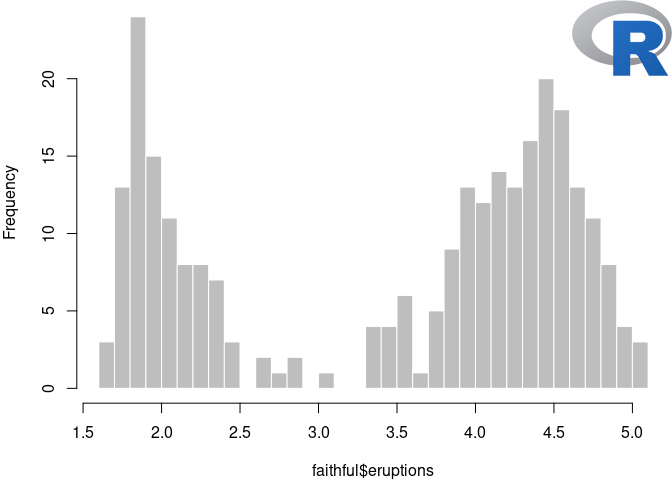
\includegraphics[width=1\linewidth,height=1\textheight,keepaspectratio]{rmarkdown-cookbook_files/figure-latex/magick-logo-1} 

}

\caption{チャンクオプション fig.process でグラフに R のロゴを追加する}\label{fig:magick-logo}
\end{figure}

あなたが \textbf{magick} パッケージにより詳しくなったら, R のグラフに後処理をするための, より創造的で有用なアイディアを思いつくことでしょう.

最後に, \texttt{fig.process} オプションのもう1つの応用例をお見せします. 以下の \texttt{pdf2png()} 関数は PDF 画像を PNG に変換します. \ref{graphical-device}節ではグラフの生成のために \texttt{tikz} グラフィックデバイスを使用する例を見せました. この方法の問題は, デバイスが PDF を生成することで, LaTeX でない出力の文書に対しては機能しないということです. チャンクオプション \texttt{dev = "tikz"} と \texttt{fig.process = pdf2png} で, グラフの PNG 版を図\ref{fig:dev-tikz}に示すことができます.

\begin{Shaded}
\begin{Highlighting}[numbers=left,,]
\NormalTok{pdf2png }\OtherTok{\textless{}{-}} \ControlFlowTok{function}\NormalTok{(path) \{}
  \CommentTok{\# LaTeX でない出力に対してのみ変換する}
  \ControlFlowTok{if}\NormalTok{ (knitr}\SpecialCharTok{::}\FunctionTok{is\_latex\_output}\NormalTok{()) }
    \FunctionTok{return}\NormalTok{(path)}
\NormalTok{  path2 }\OtherTok{\textless{}{-}}\NormalTok{ xfun}\SpecialCharTok{::}\FunctionTok{with\_ext}\NormalTok{(path, }\StringTok{"png"}\NormalTok{)}
\NormalTok{  img }\OtherTok{\textless{}{-}}\NormalTok{ magick}\SpecialCharTok{::}\FunctionTok{image\_read\_pdf}\NormalTok{(path)}
\NormalTok{  magick}\SpecialCharTok{::}\FunctionTok{image\_write}\NormalTok{(img, path2, }\AttributeTok{format =} \StringTok{"png"}\NormalTok{)}
\NormalTok{  path2}
\NormalTok{\}}
\end{Highlighting}
\end{Shaded}

\hypertarget{graphical-device}{%
\section{高品質なグラフィック (*)}\label{graphical-device}}

\textbf{rmarkdown} パッケージはそれぞれの出力フォーマットに対して妥当なデフォルトのグラフィックデバイスを設定しています. 例えば HTML 出力に対しては \texttt{png()} を使うので, \textbf{knitr} は PNG 画像ファイルを生成し, PDF 出力に対しては \texttt{pdf()} デバイスを使う, などです. あなたがデフォルトのグラフィックデバイスの品質に不満なら, チャンクオプション \texttt{dev}\index{チャンクオプション!dev} によって変更することができます. \textbf{knitr} によってサポートされているグラフィックデバイスの一覧は次のようになります. \texttt{"bmp"}, \texttt{"postscript"}, \texttt{"pdf"}, \texttt{"png"}, \texttt{"svg"}, \texttt{"jpeg"}, \texttt{"pictex"}, \texttt{"tiff"}, \texttt{"win.metafile"}, \texttt{"cairo\_pdf"}, \texttt{"cairo\_ps"}, \texttt{"quartz\_pdf"}, \texttt{"quartz\_png"}, \texttt{"quartz\_jpeg"}, \texttt{"quartz\_tiff"}, \texttt{"quartz\_gif"}, \texttt{"quartz\_psd"}, \texttt{"quartz\_bmp"}, \texttt{"CairoJPEG"}, \texttt{"CairoPNG"}, \texttt{"CairoPS"}, \texttt{"CairoPDF"}, \texttt{"CairoSVG"}, \texttt{"CairoTIFF"}, \texttt{"Cairo\_pdf"}, \texttt{"Cairo\_png"}, \texttt{"Cairo\_ps"}, \texttt{"Cairo\_svg"}, \texttt{"svglite"}, \texttt{"ragg\_png"}, and \texttt{"tikz"}

大抵の場合, グラフィックデバイスの名前は関数名でもあります. デバイス\index{図!デバイス}についてもっと詳しく知りたいなら, あなたは R のヘルプページを読むことができます. 例えば \texttt{svg} デバイスの詳細を知るのに, R コンソールで \texttt{?svg} と打つことができます. このデバイスは base R に含まれています. さらに \texttt{quartz\_XXX} デバイスは \texttt{quartz()} 関数を元にしたもので, macOS でのみ有効です. \texttt{CairoXXX} デバイスは \textbf{Cairo} \autocite{R-Cairo} パッケージによるアドオンで, \texttt{Cairo\_XXX} デバイスは \textbf{cairoDevice} package \autocite{R-cairoDevice} から\footnote{\textbf{訳注}: これらと異なり, \texttt{cairo\_pdf} は base R に含まれています.}, \texttt{svglite} デバイスは \textbf{svglite} パッケージ \autocite{R-svglite} から, \texttt{tikz} は \textbf{tikzDevice} パッケージ \autocite{R-tikzDevice} からのデバイスです. アドオンパッケージ由来のデバイスを使いたいなら, そのパッケージをまずインストールしなければなりません.\index{R パッケージ!グラフィックデバイス}

大抵はベクタ画像はラスタ画像よりも高品質であり, ベクタ画像は品質を損なうことなく縮尺を変更できます. HTML 出力では, SVG のグラフのために \texttt{dev = "svg"} または \texttt{dev = "svglite"} を使うことを検討してください. SVG はベクタ画像形式で, デフォルトの \texttt{png} デバイスはラスタ画像形式であることに注意してください.

あなたが PDF 出力時のグラフ内の書体に対してこだわりが強い人なら, \texttt{dev = "tikz"} を使うこともできます. これは LaTeX がネイティヴでサポートしているからです. つまり, テキストや記号を含むグラフの全ての要素が LaTeX を介して高品質にレンダリングされるということです. 図\ref{fig:dev-tikz}に, \texttt{dev = "tikz"} で R のグラフ内で LaTeX 数式表現を書く例を示します.

\begin{Shaded}
\begin{Highlighting}[numbers=left,,]
\FunctionTok{par}\NormalTok{(}\AttributeTok{mar =} \FunctionTok{c}\NormalTok{(}\DecValTok{4}\NormalTok{, }\DecValTok{4}\NormalTok{, }\DecValTok{2}\NormalTok{, .}\DecValTok{1}\NormalTok{))}
\FunctionTok{curve}\NormalTok{(dnorm, }\SpecialCharTok{{-}}\DecValTok{3}\NormalTok{, }\DecValTok{3}\NormalTok{, }\AttributeTok{xlab =} \StringTok{\textquotesingle{}$x$\textquotesingle{}}\NormalTok{, }\AttributeTok{ylab =} \StringTok{\textquotesingle{}$}\SpecialCharTok{\textbackslash{}\textbackslash{}}\StringTok{phi(x)$\textquotesingle{}}\NormalTok{,}
      \AttributeTok{main =} \StringTok{\textquotesingle{}The density function of $N(0, 1)$\textquotesingle{}}\NormalTok{)}
\FunctionTok{text}\NormalTok{(}\SpecialCharTok{{-}}\DecValTok{1}\NormalTok{, .}\DecValTok{2}\NormalTok{, }\AttributeTok{cex =} \DecValTok{3}\NormalTok{, }\AttributeTok{col =} \StringTok{\textquotesingle{}blue\textquotesingle{}}\NormalTok{,}
  \StringTok{\textquotesingle{}$}\SpecialCharTok{\textbackslash{}\textbackslash{}}\StringTok{phi(x)=}\SpecialCharTok{\textbackslash{}\textbackslash{}}\StringTok{frac\{1\}\{}\SpecialCharTok{\textbackslash{}\textbackslash{}}\StringTok{sqrt\{2}\SpecialCharTok{\textbackslash{}\textbackslash{}}\StringTok{pi\}\}e\^{}\{}\SpecialCharTok{\textbackslash{}\textbackslash{}}\StringTok{frac\{{-}x\^{}2\}\{2\}\}$\textquotesingle{}}\NormalTok{)}
\end{Highlighting}
\end{Shaded}

\begin{figure}

{\centering 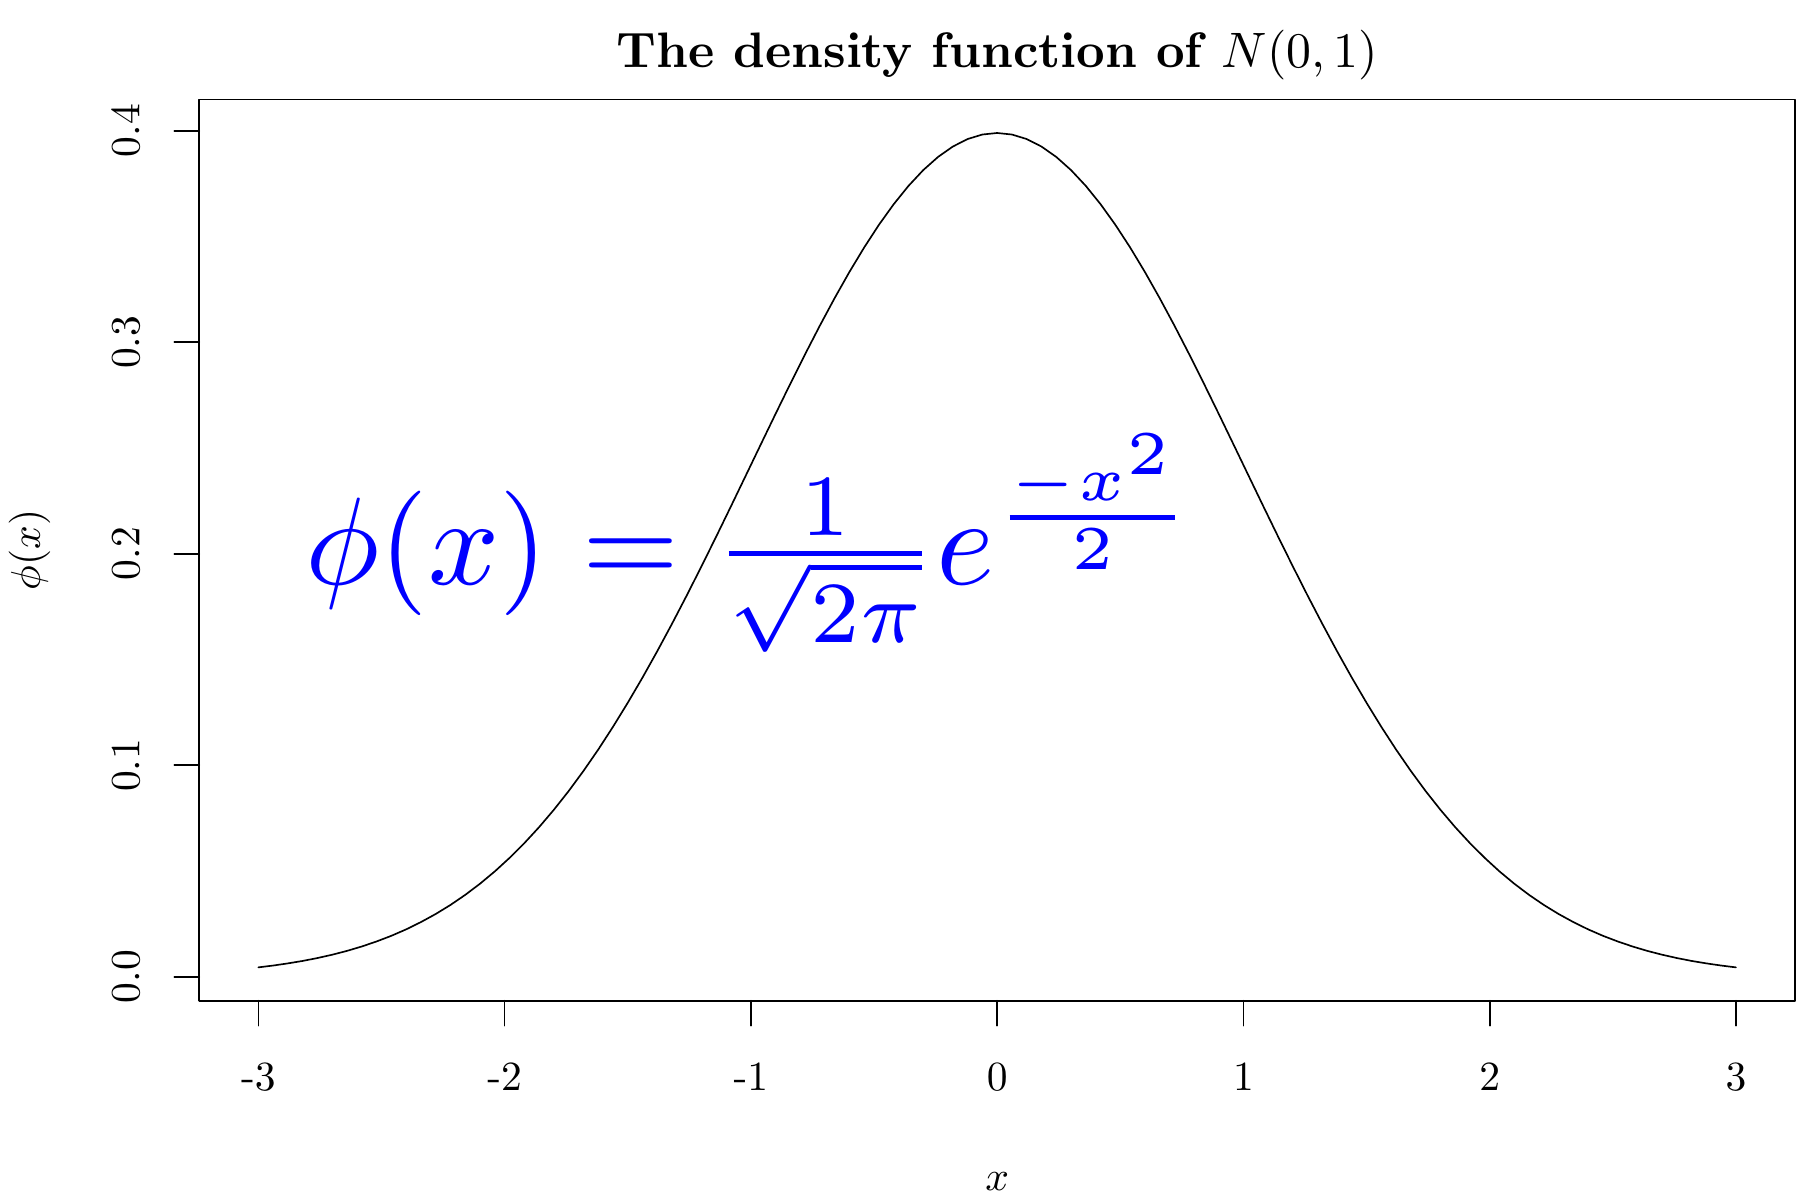
\includegraphics[width=1\linewidth,height=1\textheight,keepaspectratio]{rmarkdown-cookbook_files/figure-latex/dev-tikz-1} 

}

\caption{tikz デバイスでレンダリングされたグラフ}\label{fig:dev-tikz}
\end{figure}

base R は実は数式表現をサポートしていますが, LaTeX を介してレンダリングされていないことに注意してください (詳細は \texttt{?plotmath} を見てください). \texttt{tikz} デバイスの細かい組版を調整するいくつかの発展的なオプションがあります. \texttt{?tikzDevice::tikz} で, できることを確認することもできます. 例えばグラフにマルチバイト文字が含まれているなら, このオプションを設定することができます.

\begin{Shaded}
\begin{Highlighting}[numbers=left,,]
\FunctionTok{options}\NormalTok{(}\AttributeTok{tikzDefaultEngine =} \StringTok{"xetex"}\NormalTok{)}
\end{Highlighting}
\end{Shaded}

これは, LaTeX 文書でマルチバイト文字を処理する観点で, \texttt{xetex} の方が大抵の場合はデフォルトのエンジン \texttt{pdftex} より優れているからです.

\texttt{tikz} の主な欠点が2つあります. 1つ目は LaTeX のインストールが必要ということですが, これはそこまで深刻ではありません (\ref{install-latex}節参照). 他にもいくつかの LaTeX パッケージが必要になりますが, TinyTeX を使用しているなら簡単にインストールできます.

\begin{Shaded}
\begin{Highlighting}[numbers=left,,]
\NormalTok{tinytex}\SpecialCharTok{::}\FunctionTok{tlmgr\_install}\NormalTok{(}\FunctionTok{c}\NormalTok{(}\StringTok{"pgf"}\NormalTok{, }\StringTok{"preview"}\NormalTok{, }\StringTok{"xcolor"}\NormalTok{))}
\end{Highlighting}
\end{Shaded}

2つ目の欠点は, デバイスが LaTeX ファイルを生成してから PDF にコンパイルするため, グラフのレンダリングが顕著に遅くなるということです. コードチャンクに時間がかかると感じるなら, \texttt{cache = TRUE} でチャンクオプションを有効にすることもできます (\ref{cache}節参照).

図\ref{fig:dev-tikz}には, チャンクオプション \texttt{fig.process = pdf2png}\index{チャンクオプション!fig.process} が使われています. \texttt{pdf2png} は\ref{fig-process}節で定義された, 出力フォーマットが LaTeX でない時に PDF 画像を PNG に変換するものです. 変換しない場合, 本書のオンライン版をウエブブラウザで閲覧しても PDF グラフは見られないでしょう.

\hypertarget{low-plots}{%
\section{低水準作図関数で1つづつグラフを作る (*)}\label{low-plots}}

R グラフィックスには2種類の作図関数があります. 高水準作図関数は新たなグラフを作成し, 低水準作図関数は既存のグラフに要素を追加します. 詳細は R マニュアルの12章 \href{https://cran.r-project.org/doc/manuals/r-release/R-intro.html}{\emph{An Introduction to R}} を確認することもできます.

デフォルトでは \textbf{knitr} は低水準作図関数による中間グラフ\index{図!中間グラフ}はそれより前のグラフを修正するのに使います. 全ての低水準作図による変更が反映された最後のグラフのみが表示されます. By default, \textbf{knitr} does not show the intermediate plots when a series of low-level plotting functions\index{figure!intermediate plots} are used to modify a previous plot. Only the last plot on which all low-level plotting changes have been made is shown.

特に教育目的では, 中間グラフを表示することが有用になりえます. 低水準作図による変更を保存するために, チャンクオプション \texttt{fig.keep = \textquotesingle{}low\textquotesingle{}}\index{チャンクオプション!fig.keep} を設定することができます. 例えば 図\ref{fig:low-plots-1}, \ref{fig:low-plots-2}は \texttt{fig.keep = \textquotesingle{}low\textquotesingle{}} のオプションを設定した同一のコードチャンク由来ですが, 2つのコードチャンクから生成されたように見えます. さらに異なる図のキャプションを, チャンクオプション \texttt{fig.cap = c(\textquotesingle{}...の散布図\textquotesingle{},\ \textquotesingle{}...\ に回帰直線を追加\textquotesingle{})} で割り当てています.\index{チャンクオプション!fig.cap}

\begin{Shaded}
\begin{Highlighting}[numbers=left,,]
\FunctionTok{par}\NormalTok{(}\AttributeTok{mar =} \FunctionTok{c}\NormalTok{(}\DecValTok{4}\NormalTok{, }\DecValTok{4}\NormalTok{, }\FloatTok{0.1}\NormalTok{, }\FloatTok{0.1}\NormalTok{))}
\FunctionTok{plot}\NormalTok{(cars)}
\end{Highlighting}
\end{Shaded}

\begin{figure}

{\centering 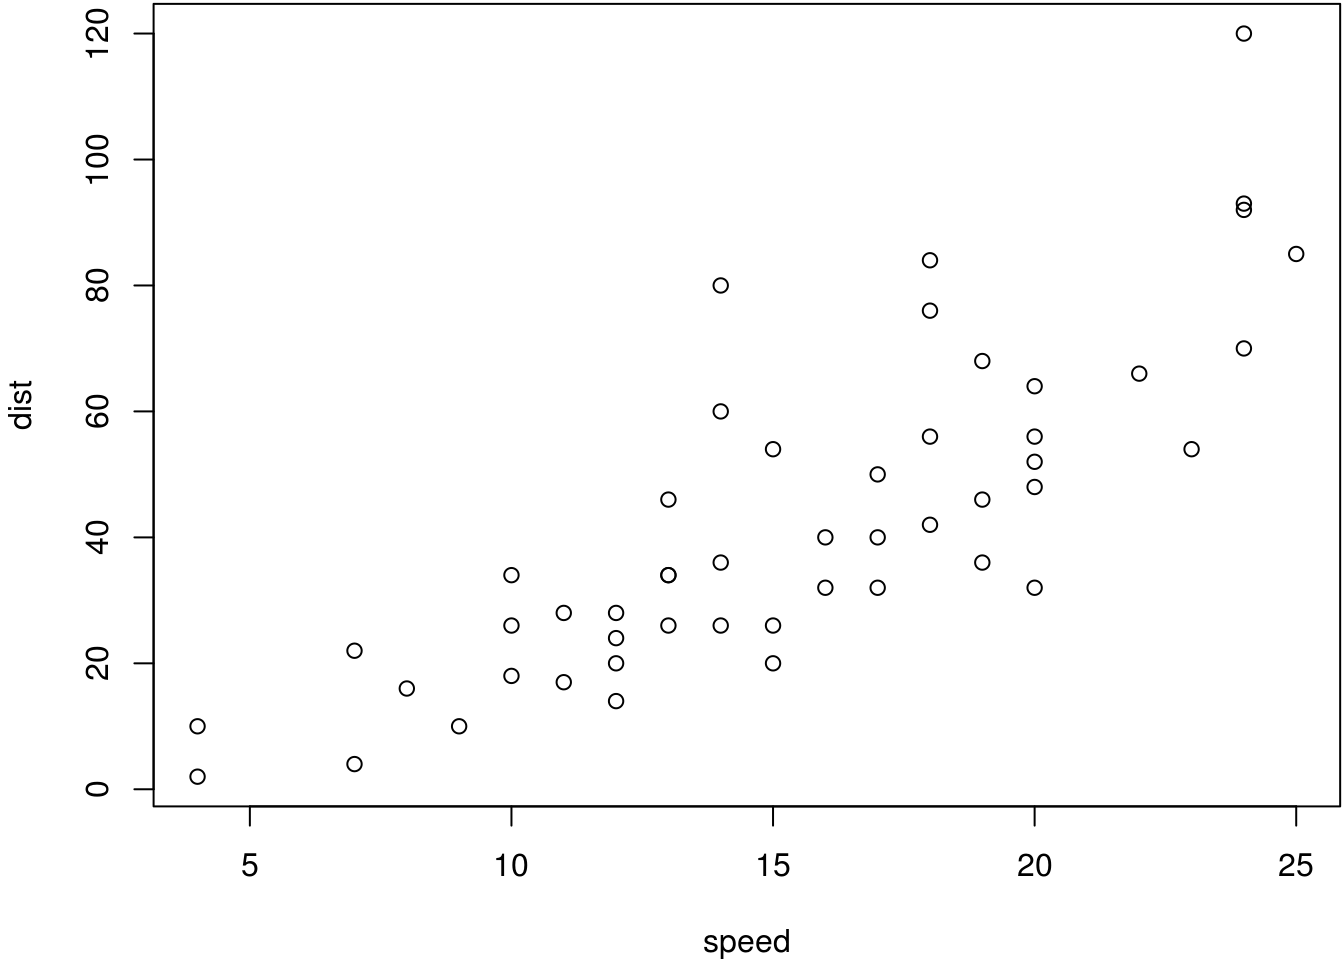
\includegraphics[width=1\linewidth,height=1\textheight,keepaspectratio]{rmarkdown-cookbook_files/figure-latex/low-plots-1} 

}

\caption{cars データの散布図.}\label{fig:low-plots-1}
\end{figure}

\begin{Shaded}
\begin{Highlighting}[numbers=left,,]
\NormalTok{fit }\OtherTok{\textless{}{-}} \FunctionTok{lm}\NormalTok{(dist }\SpecialCharTok{\textasciitilde{}}\NormalTok{ speed, }\AttributeTok{data =}\NormalTok{ cars)}
\FunctionTok{abline}\NormalTok{(fit)}
\end{Highlighting}
\end{Shaded}

\begin{figure}

{\centering 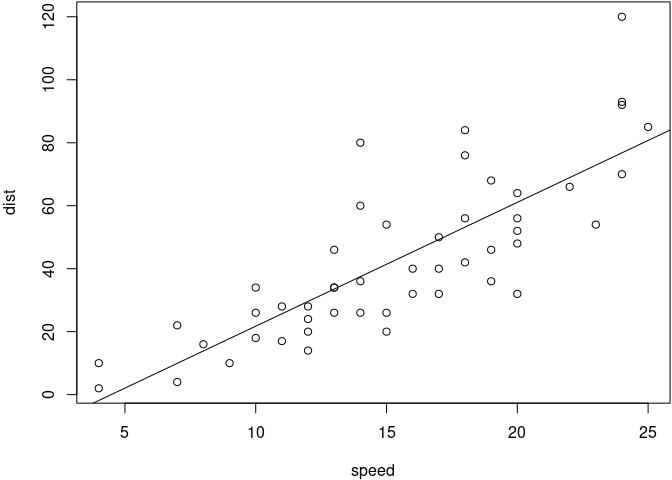
\includegraphics[width=1\linewidth,height=1\textheight,keepaspectratio]{rmarkdown-cookbook_files/figure-latex/low-plots-2} 

}

\caption{既にある散布図に回帰曲線を追加}\label{fig:low-plots-2}
\end{figure}

\textbf{異なる}コードチャンク間でグラフの変更を維持したいなら, \ref{global-device}節を参照してください.

\hypertarget{opts-render}{%
\section{チャンク内のオブジェクト表示をカスタマイズする (*)}\label{opts-render}}

デフォルトではコードチャンク内のオブジェクトは \texttt{knitr::knit\_print()}\index{knitr!knit\_print()} 関数を通して表示され, これは概ね base R の \texttt{print()} と同じです. \texttt{knit\_print()} 関数は S3 ジェネリック関数であり, あなたが自分で S3 メソッドを登録することで機能を拡張できることを意味します. 以下は \texttt{knitr::kable()} でデータフレームを表として自動的に表示する方法の例を示しています.

\begin{Shaded}
\begin{Highlighting}[]
\CommentTok{{-}{-}{-}}
\AnnotationTok{title:}\CommentTok{ データフレームの表示にカスタム \textasciigrave{}knit\_print\textasciigrave{} メソッドを使う}
\CommentTok{{-}{-}{-}}

\NormalTok{初めに }\InformationTok{\textasciigrave{}knit\_print\textasciigrave{}}\NormalTok{ メソッドを定義して登録します.}

\InformationTok{\textasciigrave{}\textasciigrave{}\textasciigrave{}\{r\}}
\InformationTok{knit\_print.data.frame = function(x, ...) \{}
\InformationTok{  res = paste(c("", "", knitr::kable(x)), collapse = "\textbackslash{}n")}
\InformationTok{  knitr::asis\_output(res)}
\InformationTok{\}}

\InformationTok{registerS3method(}
\InformationTok{  "knit\_print", "data.frame", knit\_print.data.frame,}
\InformationTok{  envir = asNamespace("knitr")}
\InformationTok{)}
\InformationTok{\textasciigrave{}\textasciigrave{}\textasciigrave{}}

\NormalTok{これでデータフレームに対するカスタム表示メソッドをテストできます. もはや }\InformationTok{\textasciigrave{}knitr::kable()\textasciigrave{}}\NormalTok{ を明示的に呼ぶ必要がないことに注意してください.}

\InformationTok{\textasciigrave{}\textasciigrave{}\textasciigrave{}\{r\}}
\InformationTok{head(iris)}
\InformationTok{\textasciigrave{}\textasciigrave{}\textasciigrave{}}

\InformationTok{\textasciigrave{}\textasciigrave{}\textasciigrave{}\{r\}}
\InformationTok{head(mtcars)}
\InformationTok{\textasciigrave{}\textasciigrave{}\textasciigrave{}}
\end{Highlighting}
\end{Shaded}

\texttt{knit\_print()} 関数の詳細は \textbf{knitr} パッケージ\index{R パッケージ!knitr}のビネットから学ぶことができます.

\begin{Shaded}
\begin{Highlighting}[numbers=left,,]
\FunctionTok{vignette}\NormalTok{(}\StringTok{"knit\_print"}\NormalTok{, }\AttributeTok{package =} \StringTok{"knitr"}\NormalTok{)}
\end{Highlighting}
\end{Shaded}

\textbf{printr} パッケージ\index{R パッケージ!printr} \autocite{R-printr} はいくつかの R オブジェクトを可能な範囲で自動的に表として表示する S3 メソッドをいくつか提供します. コードチャンクで \texttt{library(printr)} を実行するだけで十分で, 全てのメソッドが自動的に登録されます.

このテクニックがとても上級者向けだと感じたなら, \texttt{html\_document} や \texttt{pdf\_document} のような R Markdown の出力フォーマットに \texttt{df\_print} オプションを与えてください. これでデータフレームの表示に関する挙動をカスタマイズできます. 例えばデータフレームを \texttt{knitr::kable()} で表示したいなら, このようにオプションを設定することもできます.

\begin{Shaded}
\begin{Highlighting}[]
\PreprocessorTok{{-}{-}{-}}
\FunctionTok{output}\KeywordTok{:}
\AttributeTok{  }\FunctionTok{html\_document}\KeywordTok{:}
\AttributeTok{    }\FunctionTok{df\_print}\KeywordTok{:}\AttributeTok{ kable}
\PreprocessorTok{{-}{-}{-}}
\end{Highlighting}
\end{Shaded}

出力フォーマットが \texttt{df\_print} をサポートするかどうか, そしてもしそうなら使用可能な値が何であるかの判断は, 出力フォーマット関数のヘルプページを見てください.

実際には, \texttt{render} チャンクオプションで \texttt{knit\_print()} 関数を完全に置き換えることができます. このオプションはオブジェクトを表示する任意の関数を取ることができます. 例えば \textbf{pander} パッケージ\index{R パッケージ!pander} を使用するオブジェクトを表示したいなら, チャンクオプション \texttt{render} に \texttt{pander::pander()} を設定することもできます.

\begin{Shaded}
\begin{Highlighting}[]
\InformationTok{\textasciigrave{}\textasciigrave{}\textasciigrave{}\{r, render=pander::pander\}}
\InformationTok{iris}
\InformationTok{\textasciigrave{}\textasciigrave{}\textasciigrave{}}
\end{Highlighting}
\end{Shaded}

\texttt{render} オプションによって, あなたは R オブジェクトの表示方法に対する完全なる自由を手に入れるでしょう.

\hypertarget{option-hooks}{%
\section{オプションフック (*)}\label{option-hooks}}

あるチャンクオプションを, 他のチャンクオプションの値に応じて動的に変えたい\index{チャンクオプション!オプションフック}\index{オプションフック}ことがあるかもしれません. これを実施するには\textbf{オプションフック}を設定するために, \texttt{opts\_hooks} オブジェクトを使用することもできます. オプションフックはオプションと関連付けられた関数で, 対応するチャンクオプションが \texttt{NULL} でないときに実行されます. この関数は現在のチャンクのオプションのリストを引数として受け取り, そのリストを (おそらく変更して) 返すものであるべきです. 例えば \texttt{fig.width} オプションを常に \texttt{fig.height} より小さくならないように調整することができます.

\begin{Shaded}
\begin{Highlighting}[numbers=left,,]
\NormalTok{knitr}\SpecialCharTok{::}\NormalTok{opts\_hooks}\SpecialCharTok{$}\FunctionTok{set}\NormalTok{(}\AttributeTok{fig.width =} \ControlFlowTok{function}\NormalTok{(options) \{}
  \ControlFlowTok{if}\NormalTok{ (options}\SpecialCharTok{$}\NormalTok{fig.width }\SpecialCharTok{\textless{}}\NormalTok{ options}\SpecialCharTok{$}\NormalTok{fig.height) \{}
\NormalTok{    options}\SpecialCharTok{$}\NormalTok{fig.width }\OtherTok{\textless{}{-}}\NormalTok{ options}\SpecialCharTok{$}\NormalTok{fig.height}
\NormalTok{  \}}
\NormalTok{  options}
\NormalTok{\})}
\end{Highlighting}
\end{Shaded}

\texttt{fig.width} が \texttt{NULL} になることはないので, このフック関数は常に, コードチャンクの直前にチャンクオプションの更新のために実行されます. 以下のコードチャンクは, 上記のオプションフックが設定されていれば, \texttt{fig.width} が初期値の5の代わりに実際には6になります.

\begin{Shaded}
\begin{Highlighting}[]
\InformationTok{\textasciigrave{}\textasciigrave{}\textasciigrave{}\{r fig.width = 5, fig.height = 6\}}
\InformationTok{plot(1:10)}
\InformationTok{\textasciigrave{}\textasciigrave{}\textasciigrave{}}
\end{Highlighting}
\end{Shaded}

別の例として, \ref{opts-comment}説の最後の例を書き換えます. 単一のチャンクオプション \texttt{console = TRUE} が, \texttt{comment = ""} と \texttt{prompt = TRUE} を意味するようにできます. \texttt{console} は \textbf{knitr} の固有のチャンクオプションでなく, 任意の名前のカスタムオプションであることに注意してください. デフォルト値は \texttt{NULL} です. 以下はその完全な例です.

\begin{Shaded}
\begin{Highlighting}[]
\InformationTok{\textasciigrave{}\textasciigrave{}\textasciigrave{}\{r, include=FALSE\}}
\InformationTok{knitr::opts\_hooks$set(console = function(options) \{}
\InformationTok{  if (isTRUE(options$console)) \{}
\InformationTok{    options$comment \textless{}{-} \textquotesingle{}\textquotesingle{}; options$prompt \textless{}{-} TRUE}
\InformationTok{  \}}
\InformationTok{  options}
\InformationTok{\})}
\InformationTok{\textasciigrave{}\textasciigrave{}\textasciigrave{}}

\NormalTok{デフォルトの出力.}

\InformationTok{\textasciigrave{}\textasciigrave{}\textasciigrave{}\{r\}}
\InformationTok{1 + 1}
\InformationTok{if (TRUE) \{}
\InformationTok{  2 + 2}
\InformationTok{\}}
\InformationTok{\textasciigrave{}\textasciigrave{}\textasciigrave{}}

\InformationTok{\textasciigrave{}console = TRUE\textasciigrave{}}\NormalTok{ で出力.}

\InformationTok{\textasciigrave{}\textasciigrave{}\textasciigrave{}\{r, console=TRUE\}}
\InformationTok{1 + 1}
\InformationTok{if (TRUE) \{}
\InformationTok{  2 + 2}
\InformationTok{\}}
\InformationTok{\textasciigrave{}\textasciigrave{}\textasciigrave{}}
\end{Highlighting}
\end{Shaded}

3つ目の例はどうやって自動的にソースコード・テキスト出力・メッセージ・警告・エラーの出力ブロックに行番号を追加するかに関するものです. 行番号を追加するために \texttt{attr.source}, \texttt{attr.output} といったチャンクオプションを使用する方法は\ref{number-lines}節で紹介しています. ここでは単一のチャンクオプション (この例では \texttt{numberLines}) で行番号を追加するかどうかを制御したいとします.

\begin{Shaded}
\begin{Highlighting}[numbers=left,,]
\NormalTok{knitr}\SpecialCharTok{::}\NormalTok{opts\_hooks}\SpecialCharTok{$}\FunctionTok{set}\NormalTok{(}
  \AttributeTok{numberLines =} \ControlFlowTok{function}\NormalTok{(options) \{}
\NormalTok{    attrs }\OtherTok{\textless{}{-}} \FunctionTok{paste0}\NormalTok{(}\StringTok{"attr."}\NormalTok{, options}\SpecialCharTok{$}\NormalTok{numberLines)}
\NormalTok{    options[attrs] }\OtherTok{\textless{}{-}} \FunctionTok{lapply}\NormalTok{(options[attrs], c, }\StringTok{".numberLines"}\NormalTok{)}
\NormalTok{    options}
\NormalTok{  \}}
\NormalTok{)}

\NormalTok{knitr}\SpecialCharTok{::}\NormalTok{opts\_chunk}\SpecialCharTok{$}\FunctionTok{set}\NormalTok{(}
  \AttributeTok{numberLines =} \FunctionTok{c}\NormalTok{(}
    \StringTok{"source"}\NormalTok{, }\StringTok{"output"}\NormalTok{, }\StringTok{"message"}\NormalTok{, }\StringTok{"warning"}\NormalTok{, }\StringTok{"error"}
\NormalTok{  )}
\NormalTok{)}
\end{Highlighting}
\end{Shaded}

基本的に, オプションフック \texttt{numberLines} は \texttt{.numberLines} 属性を出力ブロックに追加し, チャンクオプション \texttt{opts\_chunk\$set()} によって設定された \texttt{numberLunes} はオプションフックによって実行されたことが確認されます.

上記の設定では, チャンクオプション \texttt{numberLines} をコードチャンクで使用して, そのチャンクの出力ブロックのどの部分に行番号を付けるかを決めることができます. 例えば \texttt{numberLines = c(\textquotesingle{}source\textquotesingle{},\ \textquotesingle{}output\textquotesingle{})} のように. \texttt{numberLines = NULL} は行番号を完全に削除します.

このアプローチがチャンクオプションを直接設定するのと何が違うのかと思うかもしれません. 例えば\ref{number-lines}節でしたように, 単に \texttt{knitr::opts\_chunk\$set(attr.source = \textquotesingle{}.numberLines\textquotesingle{})} とする場合と. ここでオプションフックを使う利点は \texttt{.numberLines} 属性をチャンクオプションに\textbf{追加する}という点のみです. これはチャンクオプションの既に存在する値を\textbf{上書きする}ことを意味しません. 例えば以下のチャンクのソースコードブロックは (既に設定したため) 行番号が付いており, そして番号を2行目から始めます.

\begin{Shaded}
\begin{Highlighting}[]
\InformationTok{\textasciigrave{}\textasciigrave{}\textasciigrave{}\{r, attr.source=\textquotesingle{}startFrom="2"\textquotesingle{}\}}
\InformationTok{\# このコメント行には番号がつかない}
\InformationTok{1 + 1}
\InformationTok{\textasciigrave{}\textasciigrave{}\textasciigrave{}}
\end{Highlighting}
\end{Shaded}

これは以下と同等です.

\begin{Shaded}
\begin{Highlighting}[]
\InformationTok{\textasciigrave{}\textasciigrave{}\textasciigrave{}\{r, attr.source=c(\textquotesingle{}startFrom="2"\textquotesingle{}, \textquotesingle{}.numberLines\textquotesingle{}\}}
\InformationTok{\# このコメント行には番号がつかない}
\InformationTok{1 + 1}
\InformationTok{\textasciigrave{}\textasciigrave{}\textasciigrave{}}
\end{Highlighting}
\end{Shaded}

\hypertarget{output-hooks}{%
\chapter{出力フック (*)}\label{output-hooks}}

\textbf{knitr} パッケージによって, あなたはコードチャンクから出力されるものを各パーツ, ソースコード・テキスト出力・メッセージ・グラフといったものごとに制御しています. この制御は「出力フック」\index{出力フック}\index{output hooks|see{出力フック}} (output hook(s))によって実現されています. 出力フックは出力の各パーツを入力 (典型的には文字列ベクトルとして扱います) として, 出力文書に書き出すための文字列を返す一連の関数です. 現時点ではこのしくみを理解するのは簡単ではないでしょうが, これから説明する簡単な例を見ればこのアイディアがはっきりと理解できるものと思います. この例ではコードチャンクの出力がどのようにして \textbf{knitr} の出力フックを介してレンダリングされるかを表しています.

このような1行だけのコードチャンクについて考えてみてください.

\begin{Shaded}
\begin{Highlighting}[]
\InformationTok{\textasciigrave{}\textasciigrave{}\textasciigrave{}\{r\}}
\InformationTok{1 + 1}
\InformationTok{\textasciigrave{}\textasciigrave{}\textasciigrave{}}
\end{Highlighting}
\end{Shaded}

\textbf{knitr} がコードチャンクを評価した後, 2つの出力要素を得て, 2つとも文字列ベクトルとして保持されます. ソースコードの \texttt{"1 + 1"} と, テキスト出力の \texttt{"{[}1{]}\ 2"} です. これらの文字列は求められている出力フォーマットに応じて, チャンクフックによってさらなる処理がなされます. たとえば Markdown 文書では \textbf{knitr} はソースコードを言語名を付けてコードブロックで囲みます. これは \texttt{source} フックを介して行われ, だいたいこのような関数となります.

\begin{Shaded}
\begin{Highlighting}[numbers=left,,]
\CommentTok{\# 上記のケースでは, \textasciigrave{}x\textasciigrave{} は文字列 \textquotesingle{}1 + 1\textquotesingle{} に相当}
\ControlFlowTok{function}\NormalTok{(x, options) \{}
  \CommentTok{\# ここの小文字 \textquotesingle{}r\textquotesingle{} は言語名を表す}
  \FunctionTok{paste}\NormalTok{(}\FunctionTok{c}\NormalTok{(}\StringTok{"\textasciigrave{}\textasciigrave{}\textasciigrave{}r"}\NormalTok{, x, }\StringTok{"\textasciigrave{}\textasciigrave{}\textasciigrave{}"}\NormalTok{), }\AttributeTok{collapse =} \StringTok{"}\SpecialCharTok{\textbackslash{}n}\StringTok{"}\NormalTok{)}
\NormalTok{\}}
\end{Highlighting}
\end{Shaded}

同様に, テキスト出力はこのような \texttt{output} フック関数によって処理されます.

\begin{Shaded}
\begin{Highlighting}[numbers=left,,]
\ControlFlowTok{function}\NormalTok{(x, options) \{}
  \FunctionTok{paste}\NormalTok{(}\FunctionTok{c}\NormalTok{(}\StringTok{"\textasciigrave{}\textasciigrave{}\textasciigrave{}"}\NormalTok{, x, }\StringTok{"\textasciigrave{}\textasciigrave{}\textasciigrave{}"}\NormalTok{), }\AttributeTok{collapse =} \StringTok{"}\SpecialCharTok{\textbackslash{}n}\StringTok{"}\NormalTok{)}
\NormalTok{\}}
\end{Highlighting}
\end{Shaded}

よって上記のコードチャンクの最終的な出力はこのようになります.

\begin{Shaded}
\begin{Highlighting}[]
\InformationTok{\textasciigrave{}\textasciigrave{}\textasciigrave{}r}
\DecValTok{1} \SpecialCharTok{+} \DecValTok{1}
\InformationTok{\textasciigrave{}\textasciigrave{}\textasciigrave{}}

\InformationTok{\textasciigrave{}\textasciigrave{}\textasciigrave{}}
\InformationTok{[1] 2}
\InformationTok{\textasciigrave{}\textasciigrave{}\textasciigrave{}}
\end{Highlighting}
\end{Shaded}

実際のフックは上記のような2つの関数よりも複雑ですが, 発想は同じです. \texttt{knit\_hooks}\index{knitr!knit\_hooks} オブジェクトから \texttt{get()} メソッドで実際のフック関数を取得できます. これが例です.

\begin{Shaded}
\begin{Highlighting}[numbers=left,,]
\CommentTok{\# 意味のある出力のため, 以下のコードは knitr}
\CommentTok{\# 文書のコードチャンクの *内部で* 実行されるべき}
\NormalTok{knitr}\SpecialCharTok{::}\NormalTok{knit\_hooks}\SpecialCharTok{$}\FunctionTok{get}\NormalTok{(}\StringTok{"source"}\NormalTok{)}
\NormalTok{knitr}\SpecialCharTok{::}\NormalTok{knit\_hooks}\SpecialCharTok{$}\FunctionTok{get}\NormalTok{(}\StringTok{"output"}\NormalTok{)}
\CommentTok{\# または knitr::knit\_hooks$get(c(\textquotesingle{}source\textquotesingle{}, \textquotesingle{}output\textquotesingle{}))}
\end{Highlighting}
\end{Shaded}

あなたが \textbf{knitr} パッケージの開発に貢献することに本当に関心があるのでない限り, 組み込みのフック関数のソースコードを読むことをお薦めしません. 関心があるのなら, このコードは \url{https://github.com/yihui/knitr/tree/master/R} で \texttt{hooks-*.R} という形式で命名されたスクリプトファイルにて見ることができます. 例えば \texttt{hooks-md.R} には R Markdown 文書に対するフックが含まれています. たいていの \textbf{knitr} ユーザーにとっては, 組み込みのフックよりも便利なカスタム出力フックの作り方を知っていれば十分です. この章のこれ以降では, あなたはいくつかの例で出力フックに関するこのようなことを学びます. さらに, 我々は以下のような基本的アイディアを示します.

カスタム出力フックは \texttt{knit\_hooks()} の \texttt{set()} メソッドによって登録されます. このメソッドは既存のデフォルのトフックを上書きするので, 既存のフックのコピーを保存し, 出力要素にあなた独自の処理してから, その結果をこのデフォルトのフックに与えるようにしておくことをお薦めします. 構文はたいていこのようになります.

\begin{Shaded}
\begin{Highlighting}[numbers=left,,]
\CommentTok{\# ここで local() を使うかは任意 (ここでは単に \textasciigrave{}hook\_old\textasciigrave{}}
\CommentTok{\# のような不要なグローバル変数を作ることを避ける目的)}
\FunctionTok{local}\NormalTok{(\{}
\NormalTok{  hook\_old }\OtherTok{\textless{}{-}}\NormalTok{ knitr}\SpecialCharTok{::}\NormalTok{knit\_hooks}\SpecialCharTok{$}\FunctionTok{get}\NormalTok{(}\StringTok{"NAME"}\NormalTok{)  }\CommentTok{\# 古いフックを保存する}
\NormalTok{  knitr}\SpecialCharTok{::}\NormalTok{knit\_hooks}\SpecialCharTok{$}\FunctionTok{set}\NormalTok{(}\AttributeTok{NAME =} \ControlFlowTok{function}\NormalTok{(x, options) \{}
    \CommentTok{\# ここで, x をどうしたいかにかかわらず, 新しい x を}
    \CommentTok{\# さらに古いフックに与える}
    \FunctionTok{hook\_old}\NormalTok{(x, options)}
\NormalTok{  \})}
\NormalTok{\})}
\end{Highlighting}
\end{Shaded}

ここで, \texttt{NAME} は以下のいずれかのフックの名前を意味します.

\begin{itemize}
\item
  \texttt{source}: ソースコードを処理するフック.
\item
  \texttt{output}: テキスト出力を処理するフック.
\item
  \texttt{warning}: 警告 (たいていは \texttt{warning()} で発生するもの) を処理するフック.
\item
  \texttt{message}: メッセージ (たいていは \texttt{message()} で発生するもの) を処理するフック.
\item
  \texttt{error}: エラーメッセージ (たいていは \texttt{stop()} で発生するもの) を処理するフック.
\item
  \texttt{plot}: グラフのファイルパスを処理するフック.
\item
  \texttt{inline}: インライン R コードからの出力を処理するフック.
\item
  \texttt{chunk}: チャンク全体の出力を処理するフック.
\item
  \texttt{document}: 文書全体を処理するフック.
\end{itemize}

フック関数の引数 \texttt{x} の意味は上記のリストで説明されています. \texttt{options} 引数は現在のコードチャンクのオプションのリストを意味します. 例えば \texttt{foo = TRUE} と設定したなら, フック関数内では \texttt{options\$foo} でこの値を得ることができます. \texttt{options} 引数は \texttt{inline} および \texttt{document} フックでは利用できません.

出力フックによって, チャンクと文書の出力の部品1つ1つに対して究極のコントロールを得られます. あらかじめ定義された目的を持つチャンクオプションと比較すると, 出力フックはユーザー定義関数なのではるかに強力であり, 関数内ではあなたが望むことはなんでもできます.

\hypertarget{hook-hide}{%
\section{ソースコードを検閲する}\label{hook-hide}}

ときにはレポートにソースコードの全文を掲載したくないこともあるでしょう. 例えばコードのある行にパスワードが書かれているかもしれません. \ref{hide-one}節ではチャンクオプション \texttt{echo} で R コードの文ごとに表示の有無を表せることを言及しました. 例えば \texttt{echo = 2} で2つ目の文を表示します. この節では, コードのインデックスを指定する必要のない, より柔軟な方法を提供します.

基本的なアイディアはコードに特殊なコメント, 例えば \texttt{\# 秘密!!} のようなものを追加するということです. このコメントがコードのある行から検出されると, 行を省略します. 以下は \texttt{source} フックを使用した完全な例です.

\begin{Shaded}
\begin{Highlighting}[]
\CommentTok{{-}{-}{-}}
\AnnotationTok{title:}\CommentTok{ "\textasciigrave{}source\textasciigrave{} フックを使用してコードのある行を隠す"}
\CommentTok{{-}{-}{-}}

\NormalTok{初めに, 末尾に }\InformationTok{\textasciigrave{}\# 秘密!!\textasciigrave{}}\NormalTok{ という文字列を含むコードの行を排除する }\InformationTok{\textasciigrave{}source\textasciigrave{}}\NormalTok{ フックを用意します.}

\InformationTok{\textasciigrave{}\textasciigrave{}\textasciigrave{}\{r, include=FALSE\}}
\InformationTok{local(\{}
\InformationTok{  hook\_source \textless{}{-} knitr::knit\_hooks$get(\textquotesingle{}source\textquotesingle{})}
\InformationTok{  knitr::knit\_hooks$set(source = function(x, options) \{}
\InformationTok{    x \textless{}{-} x[!grepl(\textquotesingle{}\# 秘密!!$\textquotesingle{}, x)]}
\InformationTok{    hook\_source(x, options)}
\InformationTok{  \})}
\InformationTok{\})}
\InformationTok{\textasciigrave{}\textasciigrave{}\textasciigrave{}}

\NormalTok{これで新しいフックをテストできます. この文書を knit すると, 特殊なコメント }\InformationTok{\textasciigrave{}\# 秘密!!\textasciigrave{}}\NormalTok{ のある行が見えなくなります.}

\InformationTok{\textasciigrave{}\textasciigrave{}\textasciigrave{}\{r\}}
\InformationTok{1 + 1  \# 表示されるべき通常のコード}

\InformationTok{\# 実際のユーザー名とパスワードを使ってみてください}
\InformationTok{auth \textless{}{-} httr::authenticate("user", "passwd")}
\InformationTok{auth \textless{}{-} httr::authenticate("yihui", "horsebattery")  \# 秘密!!}
\InformationTok{httr::GET("http://httpbin.org/basic{-}auth/user/passwd", auth)}
\InformationTok{\textasciigrave{}\textasciigrave{}\textasciigrave{}}
\end{Highlighting}
\end{Shaded}

上記の \texttt{source} フックの重要な部分はこの行です. これはソースコードのベクトル \texttt{x} から \texttt{grepl()} で末尾の \texttt{\# 秘密!!} とマッチングしたものを排除しています.

\begin{Shaded}
\begin{Highlighting}[numbers=left,,]
\NormalTok{x }\OtherTok{\textless{}{-}}\NormalTok{ x[}\SpecialCharTok{!}\FunctionTok{grepl}\NormalTok{(}\StringTok{"\# SECRET!!$"}\NormalTok{, x)]}
\end{Highlighting}
\end{Shaded}

正確に言うなら, 上記のフックは末尾に \texttt{\# 秘密!!} というコメントのある行ではなく, \textbf{評価式} (expressions) を全て排除します. \texttt{x} は実際には R 評価式のベクトルだからです. 例えば以下のコードチャンクを考えます.

\begin{Shaded}
\begin{Highlighting}[numbers=left,,]
\DecValTok{1} \SpecialCharTok{+} \DecValTok{1}
\ControlFlowTok{if}\NormalTok{ (}\ConstantTok{TRUE}\NormalTok{) \{}
  \CommentTok{\# SECRET!!}
  \DecValTok{1}\SpecialCharTok{:}\DecValTok{10}
\NormalTok{\}}
\end{Highlighting}
\end{Shaded}

\texttt{source} フック内の \texttt{x} の値はこうなります.

\begin{Shaded}
\begin{Highlighting}[numbers=left,,]
\FunctionTok{c}\NormalTok{(}\StringTok{"1 + 1"}\NormalTok{, }\StringTok{"if (TRUE) \{ \# SECRET!!}\SpecialCharTok{\textbackslash{}n}\StringTok{  1:10}\SpecialCharTok{\textbackslash{}n}\StringTok{\}"}\NormalTok{)}
\end{Highlighting}
\end{Shaded}

R 評価式ではなく行を隠したいなら, \texttt{x} を行ごとに分割しなければなりません. \texttt{xfun::split\_lines()}\index{xfun!split\_lines()} の使用を検討するとよいでしょう. フック関数の本体はこうなります.

\begin{Shaded}
\begin{Highlighting}[numbers=left,,]
\NormalTok{x }\OtherTok{\textless{}{-}}\NormalTok{ xfun}\SpecialCharTok{::}\FunctionTok{split\_lines}\NormalTok{(x)  }\CommentTok{\# 個別の行に分割する}
\NormalTok{x }\OtherTok{\textless{}{-}}\NormalTok{ x[}\SpecialCharTok{!}\FunctionTok{grepl}\NormalTok{(}\StringTok{"\# SECRET!!$"}\NormalTok{, x)]}
\NormalTok{x }\OtherTok{\textless{}{-}} \FunctionTok{paste}\NormalTok{(x, }\AttributeTok{collapse =} \StringTok{"}\SpecialCharTok{\textbackslash{}n}\StringTok{"}\NormalTok{)  }\CommentTok{\# 結合して1つの行にする}
\FunctionTok{hook\_source}\NormalTok{(x, options)}
\end{Highlighting}
\end{Shaded}

この例はソースコードの文字列を操作する方法を, そして \texttt{grepl()} はおそらく文字列操作の唯一の方法ではないだろう, ということを示しています. \ref{hook-number}節では他の例もお見せしています.

\hypertarget{hook-number}{%
\section{ソースコード内に行番号を追加する}\label{hook-number}}

この節では, ソースコードに行番号をコメントとして追加する \texttt{source} フックの定義の例を示します. 例えば, このコードチャンクに対するものを考えます.

\begin{Shaded}
\begin{Highlighting}[]
\InformationTok{\textasciigrave{}\textasciigrave{}\textasciigrave{}\{r\}}
\InformationTok{if (TRUE) \{}
\InformationTok{  x \textless{}{-} 1:10}
\InformationTok{  x + 1}
\InformationTok{\}}
\InformationTok{\textasciigrave{}\textasciigrave{}\textasciigrave{}}
\end{Highlighting}
\end{Shaded}

このような出力を求めているものとします.

\begin{Shaded}
\begin{Highlighting}[numbers=left,,]
\ControlFlowTok{if}\NormalTok{ (}\ConstantTok{TRUE}\NormalTok{) \{    }\CommentTok{\# 1}
\NormalTok{  x }\OtherTok{\textless{}{-}} \DecValTok{1}\SpecialCharTok{:}\DecValTok{10}    \CommentTok{\# 2}
\NormalTok{  x }\SpecialCharTok{+} \DecValTok{1}        \CommentTok{\# 3}
\NormalTok{\}              }\CommentTok{\# 4}
\end{Highlighting}
\end{Shaded}

完全な例は以下になります.

\begin{Shaded}
\begin{Highlighting}[]
\CommentTok{{-}{-}{-}}
\AnnotationTok{title:}\CommentTok{ ソースコードに行番号を追加する}
\CommentTok{{-}{-}{-}}

\NormalTok{行番号をソースコードに追加する }\InformationTok{\textasciigrave{}source\textasciigrave{}}\NormalTok{ フックを用意します.}
\NormalTok{番号は各行の末尾のコメントに現れます.}

\InformationTok{\textasciigrave{}\textasciigrave{}\textasciigrave{}\{r, include=FALSE\}}
\InformationTok{local(\{}
\InformationTok{  hook\_source \textless{}{-} knitr::knit\_hooks$get(\textquotesingle{}source\textquotesingle{})}
\InformationTok{  knitr::knit\_hooks$set(source = function(x, options) \{}
\InformationTok{    x \textless{}{-} xfun::split\_lines(x)}
\InformationTok{    n \textless{}{-} nchar(x, \textquotesingle{}width\textquotesingle{})}
\InformationTok{    i \textless{}{-} seq\_along(x)  \# 行番号}
\InformationTok{    n \textless{}{-} n + nchar(i)}
\InformationTok{    s \textless{}{-} knitr:::v\_spaces(max(n) {-} n)}
\InformationTok{    x \textless{}{-} paste(x, s, \textquotesingle{}  \# \textquotesingle{}, i, sep = \textquotesingle{}\textquotesingle{}, collapse = \textquotesingle{}\textbackslash{}n\textquotesingle{})}
\InformationTok{    hook\_source(x, options)}
\InformationTok{  \})}
\InformationTok{\})}
\InformationTok{\textasciigrave{}\textasciigrave{}\textasciigrave{}}

\NormalTok{ここで新しいフックのテストができます. この文書を knit するとき,}
\NormalTok{末尾のコメントに行番号が見られます.}

\InformationTok{\textasciigrave{}\textasciigrave{}\textasciigrave{}\{r\}}
\InformationTok{if (TRUE) \{}
\InformationTok{  x \textless{}{-} 1:10}
\InformationTok{  x + 1}
\InformationTok{\}}
\InformationTok{\textasciigrave{}\textasciigrave{}\textasciigrave{}}
\end{Highlighting}
\end{Shaded}

上記の例での主要なトリックは各行のコメントの前必要なスペースの数を決めることです. これによってコメントが右揃えになっています. この数は各行のコードに依存しています. このフック関数の意味を咀嚼することは読者に任せます. 内部で使われている関数 \texttt{knitr:::v\_spaces()}\index{knitr!v\_spaces()} は特定の長さのスペースを生成することに使われている点に注意してください. これが例です.

\begin{Shaded}
\begin{Highlighting}[numbers=left,,]
\NormalTok{knitr}\SpecialCharTok{:::}\FunctionTok{v\_spaces}\NormalTok{(}\FunctionTok{c}\NormalTok{(}\DecValTok{1}\NormalTok{, }\DecValTok{3}\NormalTok{, }\DecValTok{6}\NormalTok{, }\DecValTok{0}\NormalTok{))}
\end{Highlighting}
\end{Shaded}

\begin{verbatim}
## [1] " "      "   "    "      " ""
\end{verbatim}

\ref{number-lines}節で紹介した方法が, ソースコードに行番号を追加する方法としてあなたが本当に求めていたものかもしれません. そちらの構文はより簡潔で, ソースコードでもテキスト出力ブロックでも動作します. 上記の \texttt{source} フックのトリックは主に, カスタム関数でソースコードを操作する可能性の1つを示唆するのが狙いです.

\hypertarget{hook-scroll}{%
\section{スクロール可能なテキスト出力}\label{hook-scroll}}

\ref{html-scroll}節ではコードブロックとテキスト出力ブロックの高さを CSS で制限する方法を紹介しました. 実際には, チャンクオプション \texttt{attr.source} と \texttt{attr.output} で \texttt{style} 属性を Markdown のコードブロックに追加するというより簡単な方法があります(これらのオプションの説明は\ref{attr-output}節参照). 例えば, このようなコードに対してチャンクオプション \texttt{attr.output} を使います.

\begin{Shaded}
\begin{Highlighting}[]
\InformationTok{\textasciigrave{}\textasciigrave{}\textasciigrave{}\{r, attr.output=\textquotesingle{}style="max{-}height: 100px;"\textquotesingle{}\}}
\InformationTok{1:300}
\InformationTok{\textasciigrave{}\textasciigrave{}\textasciigrave{}}
\end{Highlighting}
\end{Shaded}

Markdown 出力はこうなります.

\begin{Shaded}
\begin{Highlighting}[]
\InformationTok{\textasciigrave{}\textasciigrave{}\textasciigrave{}r}
\DecValTok{1}\SpecialCharTok{:}\DecValTok{300}
\InformationTok{\textasciigrave{}\textasciigrave{}\textasciigrave{}}

\InformationTok{\textasciigrave{}\textasciigrave{}\textasciigrave{}\{style="max{-}height: 100px;"\}}
\InformationTok{\#\#   [1]   1   2   3   4   5   6   7   8   9  10}
\InformationTok{\#\#  [11]  11  12  13  14  15  16  17  18  19  20}
\InformationTok{\#\#  ... ...}
\InformationTok{\textasciigrave{}\textasciigrave{}\textasciigrave{}}
\end{Highlighting}
\end{Shaded}

そして, テキスト出力ブロックは Pandoc によって HTML へと変換されます.

\begin{Shaded}
\begin{Highlighting}[]
\KeywordTok{\textless{}pre}\OtherTok{ style=}\StringTok{"max{-}height: 100px;"}\KeywordTok{\textgreater{}}
\KeywordTok{\textless{}code\textgreater{}}\NormalTok{\#\#   [1]   1   2   3   4   5   6   7   8   9  10}
\NormalTok{\#\#  [11]  11  12  13  14  15  16  17  18  19  20}
\NormalTok{\#\#  ... ...}\KeywordTok{\textless{}/code\textgreater{}}
\KeywordTok{\textless{}/pre\textgreater{}}
\end{Highlighting}
\end{Shaded}

Pandoc の fenced code blocks についてより詳しく学ぶには, \url{https://pandoc.org/MANUAL.html\#fenced-code-blocks} のマニュアルを読んでください.

\texttt{attr.source} と \texttt{attr.output} オプションによって個別のコードチャンクに対して最大の高さを指定することができます. しかしこの構文は少しばかり野暮ったく, CSS と Pandoc の Markdown 構文をより理解する必要があります. 以下にカスタムチャンクオプション \texttt{max.height} と連動するカスタム \texttt{output} フックの例を示します. よって \texttt{attr.output = \textquotesingle{}style="max-height:\ 100px;"\textquotesingle{}} の代わりに \texttt{max.height = "100px"} のようなオプションを設定する必要があります. この例では \texttt{x} 引数には手を付けず, \texttt{options} 引数のみを操作しています.

\begin{Shaded}
\begin{Highlighting}[]
\CommentTok{{-}{-}{-}}
\AnnotationTok{title:}\CommentTok{ スクロール可能なコードブロック}
\AnnotationTok{output:}\CommentTok{ }
\CommentTok{  html\_document: }
\CommentTok{    highlight: tango}
\CommentTok{{-}{-}{-}}

\NormalTok{チャンクオプション }\InformationTok{\textasciigrave{}max.height\textasciigrave{}}\NormalTok{ が設定されている時, テキスト出力に }\InformationTok{\textasciigrave{}style\textasciigrave{}}\NormalTok{ 属性を追加するような }\InformationTok{\textasciigrave{}output\textasciigrave{}}\NormalTok{ フックを設定します.}

\InformationTok{\textasciigrave{}\textasciigrave{}\textasciigrave{}\{r, include=FALSE\}}
\InformationTok{options(width = 60)}
\InformationTok{local(\{}
\InformationTok{  hook\_output \textless{}{-} knitr::knit\_hooks$get(\textquotesingle{}output\textquotesingle{})}
\InformationTok{  knitr::knit\_hooks$set(output = function(x, options) \{}
\InformationTok{    if (!is.null(options$max.height)) options$attr.output \textless{}{-} c(}
\InformationTok{      options$attr.output,}
\InformationTok{      sprintf(\textquotesingle{}style="max{-}height: \%s;"\textquotesingle{}, options$max.height)}
\InformationTok{    )}
\InformationTok{    hook\_output(x, options)}
\InformationTok{  \})}
\InformationTok{\})}
\InformationTok{\textasciigrave{}\textasciigrave{}\textasciigrave{}}

\InformationTok{\textasciigrave{}max.height\textasciigrave{}}\NormalTok{ がない場合, 出力の全体が表示されます. 例えば...,}

\InformationTok{\textasciigrave{}\textasciigrave{}\textasciigrave{}\{r\}}
\InformationTok{1:100}
\InformationTok{\textasciigrave{}\textasciigrave{}\textasciigrave{}}

\NormalTok{ここで }\InformationTok{\textasciigrave{}max.height\textasciigrave{}}\NormalTok{ に }\InformationTok{\textasciigrave{}100px\textasciigrave{}}\NormalTok{ を設定します. この高さは 100px を超えているので, テキスト出力にスクロールバーが現れます.}

\InformationTok{\textasciigrave{}\textasciigrave{}\textasciigrave{}\{r, max.height=\textquotesingle{}100px\textquotesingle{}\}}
\InformationTok{1:100}
\InformationTok{\textasciigrave{}\textasciigrave{}\textasciigrave{}}

\NormalTok{原則として }\InformationTok{\textasciigrave{}max.height\textasciigrave{}}\NormalTok{ オプションは }\InformationTok{\textasciigrave{}attr.output\textasciigrave{}}\NormalTok{ オプションに変換されます. }\InformationTok{\textasciigrave{}attr.output\textasciigrave{}}\NormalTok{ が既に設定されていたとしても動作します. つまり }\InformationTok{\textasciigrave{}attr.output\textasciigrave{}}\NormalTok{ オプションは上書きされません. 例えば }\InformationTok{\textasciigrave{}.numberLines\textasciigrave{}}\NormalTok{ 属性を付けてテキスト出力の端に行番号を表示させてみます.}

\InformationTok{\textasciigrave{}\textasciigrave{}\textasciigrave{}\{r, max.height=\textquotesingle{}100px\textquotesingle{}, attr.output=\textquotesingle{}.numberLines\textquotesingle{}\}}
\InformationTok{1:100}
\InformationTok{\textasciigrave{}\textasciigrave{}\textasciigrave{}}
\end{Highlighting}
\end{Shaded}

図\ref{fig:hook-scroll}がその出力です. チャンクオプション \texttt{attr.output} のある最後のコードチャンクでは, \texttt{max.height} によって生成された \texttt{style} 属性を既存の属性に結合することで, 既存の属性を尊重しているので, \texttt{max.height} は上書きされないことに注意してください.

\begin{Shaded}
\begin{Highlighting}[numbers=left,,]
\NormalTok{options}\SpecialCharTok{$}\NormalTok{attr.output }\OtherTok{\textless{}{-}} \FunctionTok{c}\NormalTok{(}
\NormalTok{  options}\SpecialCharTok{$}\NormalTok{attr.output,}
  \FunctionTok{sprintf}\NormalTok{(}\StringTok{\textquotesingle{}style="max{-}height: \%s;"\textquotesingle{}}\NormalTok{, options}\SpecialCharTok{$}\NormalTok{max.height)}
\NormalTok{)}
\end{Highlighting}
\end{Shaded}

\begin{figure}

{\centering 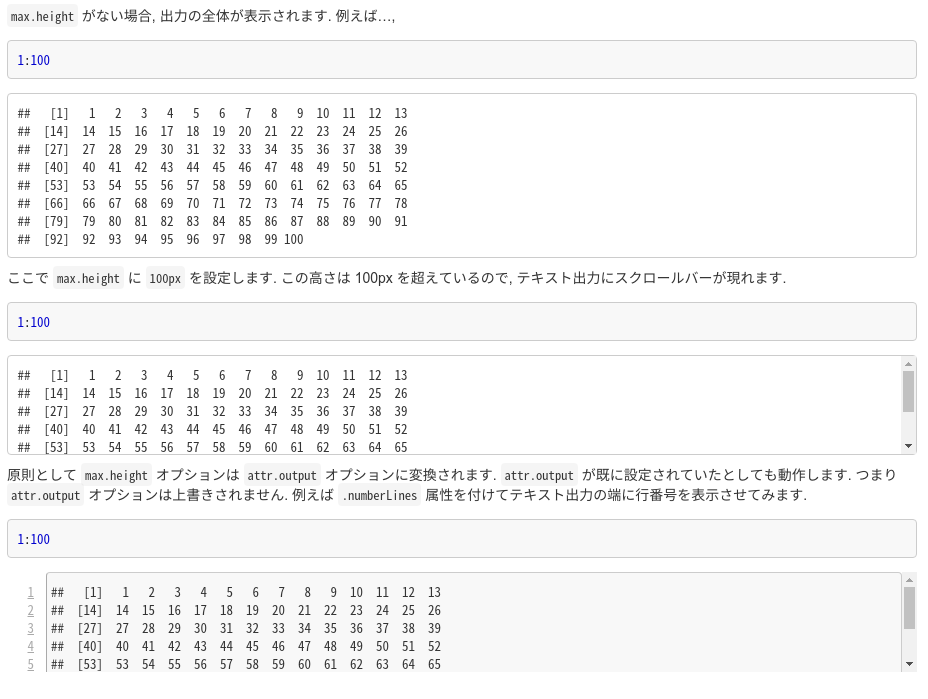
\includegraphics[width=1\linewidth,height=1\textheight,keepaspectratio]{JP/images/hook-scroll} 

}

\caption{チャンクオプション max.height を指定した, スクロール可能なテキスト出力の例}\label{fig:hook-scroll}
\end{figure}

\texttt{source} フックでもソースコードブロックの高さを制限する同様のトリックが使えます.

\hypertarget{hook-truncate}{%
\section{テキスト出力を中断する}\label{hook-truncate}}

コードチャンクから出力されたテキストが長い時, 最初の数行だけを表示させたくなるかもしれません. 例えば数千行のデータフレームを表示する時, データ全体を表示するのは不便で, 最初の数行だけで十分かもしれません. 以下では \texttt{output} フックを再定義してカスタムチャンクオプション \texttt{out.lines} によって最大行数を制御できるようにしています.

\begin{Shaded}
\begin{Highlighting}[numbers=left,,]
\CommentTok{\# 組み込みの出力フックを保存}
\NormalTok{hook\_output }\OtherTok{\textless{}{-}}\NormalTok{ knitr}\SpecialCharTok{::}\NormalTok{knit\_hooks}\SpecialCharTok{$}\FunctionTok{get}\NormalTok{(}\StringTok{"output"}\NormalTok{)}

\CommentTok{\# テキスト出力を打ち切る出力フックを新規に作成}
\NormalTok{knitr}\SpecialCharTok{::}\NormalTok{knit\_hooks}\SpecialCharTok{$}\FunctionTok{set}\NormalTok{(}\AttributeTok{output =} \ControlFlowTok{function}\NormalTok{(x, options) \{}
  \ControlFlowTok{if}\NormalTok{ (}\SpecialCharTok{!}\FunctionTok{is.null}\NormalTok{(n }\OtherTok{\textless{}{-}}\NormalTok{ options}\SpecialCharTok{$}\NormalTok{out.lines)) \{}
\NormalTok{    x }\OtherTok{\textless{}{-}}\NormalTok{ xfun}\SpecialCharTok{::}\FunctionTok{split\_lines}\NormalTok{(x)}
    \ControlFlowTok{if}\NormalTok{ (}\FunctionTok{length}\NormalTok{(x) }\SpecialCharTok{\textgreater{}}\NormalTok{ n) \{}
      \CommentTok{\# 出力を切断}
\NormalTok{      x }\OtherTok{\textless{}{-}} \FunctionTok{c}\NormalTok{(}\FunctionTok{head}\NormalTok{(x, n), }\StringTok{"....}\SpecialCharTok{\textbackslash{}n}\StringTok{"}\NormalTok{)}
\NormalTok{    \}}
\NormalTok{    x }\OtherTok{\textless{}{-}} \FunctionTok{paste}\NormalTok{(x, }\AttributeTok{collapse =} \StringTok{"}\SpecialCharTok{\textbackslash{}n}\StringTok{"}\NormalTok{)}
\NormalTok{  \}}
  \FunctionTok{hook\_output}\NormalTok{(x, options)}
\NormalTok{\})}
\end{Highlighting}
\end{Shaded}

上記のフック関数の基本的なアイディアはテキスト出力の行数が, チャンクオプション \texttt{out.lines}\index{チャンクオプション!out.lines}で指定したしきい値 (関数本体では変数 \texttt{n} として保存されています) を上回ったら最初の \texttt{n} 行だけを保持し, 出力が打ち切られたことを表す省略記号 (\texttt{....}) を末尾に加えます.

以下のチャンクでチャンクオプション \texttt{out.lines = 4} を設定し, この新たな \texttt{output} フックをテストできます.

\begin{Shaded}
\begin{Highlighting}[numbers=left,,]
\FunctionTok{print}\NormalTok{(cars)}
\end{Highlighting}
\end{Shaded}

\begin{verbatim}
##    speed dist
## 1      4    2
## 2      4   10
## 3      7    4
....
\end{verbatim}

そして期待通りに4行の出力が現れました. 本来の \texttt{output} フックを \texttt{hook\_output} 保存しているので, 再度 \texttt{set()} メソッド\index{knitr!knit\_hooks}を呼び出して復旧することができます.

\begin{Shaded}
\begin{Highlighting}[numbers=left,,]
\NormalTok{knitr}\SpecialCharTok{::}\NormalTok{knit\_hooks}\SpecialCharTok{$}\FunctionTok{set}\NormalTok{(}\AttributeTok{output =}\NormalTok{ hook\_output)}
\end{Highlighting}
\end{Shaded}

読者への練習問題として, 異なる方法で出力を打ち切ることに挑戦するとよいかもしれません. 最大行を決定するチャンクオプション \texttt{out.lines}\index{チャンクオプション!out.lines} を所与として, あなたは末尾ではなく中間を打ち切ることができますか? 例えば \texttt{out.lines = 10} なら, このように最初と最後の5行を残し, 中間に \texttt{....} を追加します.

\begin{verbatim}
##    speed dist
## 1      4    2
## 2      4   10
## 3      7    4
## 4      7   22
....
## 46    24   70
## 47    24   92
## 48    24   93
## 49    24  120
## 50    25   85
\end{verbatim}

出力の最終行, つまりフック関数の引数 \texttt{x} が空白行ならば, \texttt{c(head(x, n/2), \textquotesingle{}....\textquotesingle{},\ tail(x,\ n/2\ +\ 1))} のような処理が必要であることに注意してください. \texttt{+1} は最後の空白行を考慮するためです.

\hypertarget{hook-html5}{%
\section{HTML5 フォーマットで図を出力する}\label{hook-html5}}

デフォルトでは R Markdown のグラフは HTML 上で \texttt{\textless{}p\textgreater{}} または \texttt{\textless{}div\textgreater{}} タグ内の \texttt{\textless{}img\ src="..."\ /\textgreater{}} で読み込まれます. 以下の例は HTML5 の \texttt{\textless{}figure\textgreater{}} タグ\index{HTML!figure タグ}\index{図!HTML タグ}でグラフを表示する方法です.

\begin{Shaded}
\begin{Highlighting}[]
\CommentTok{{-}{-}{-}}
\AnnotationTok{title:}\CommentTok{ "\textasciigrave{}\textless{}figure\textgreater{}\textasciigrave{} タグで図を出力する"}
\AnnotationTok{output:}\CommentTok{ html\_document}
\CommentTok{{-}{-}{-}}

\NormalTok{ファイルパス }\InformationTok{\textasciigrave{}x\textasciigrave{}}\NormalTok{ とチャンクオプション }\InformationTok{\textasciigrave{}options$fig.cap\textasciigrave{}}\NormalTok{ の}
\NormalTok{図のキャプションが与えられた状態で, このようなフォーム内に}
\NormalTok{HTML5 タグ内にグラフを描きたいとします.}

\InformationTok{\textasciigrave{}\textasciigrave{}\textasciigrave{}html}
\KeywordTok{\textless{}figure\textgreater{}}
  \KeywordTok{\textless{}img}\OtherTok{ src=}\StringTok{"ファイルパス"}\OtherTok{ alt=}\StringTok{"キャプション"} \KeywordTok{/\textgreater{}}
  \KeywordTok{\textless{}figcaption\textgreater{}}\NormalTok{キャプション}\KeywordTok{\textless{}/figcaption\textgreater{}}
\KeywordTok{\textless{}/figure\textgreater{}}
\InformationTok{\textasciigrave{}\textasciigrave{}\textasciigrave{}}

\NormalTok{ここで出力フォーマットが HTML であるときのみ }\InformationTok{\textasciigrave{}plot\textasciigrave{}}\NormalTok{ フックを再定義します.}

\InformationTok{\textasciigrave{}\textasciigrave{}\textasciigrave{}\{r\}}
\InformationTok{if (knitr::is\_html\_output()) knitr::knit\_hooks$set(}
\InformationTok{  plot = function(x, options) \{}
\InformationTok{    cap  \textless{}{-} options$fig.cap  \# 図のキャプション}
\InformationTok{    tags \textless{}{-} htmltools::tags}
\InformationTok{    as.character(tags$figure(}
\InformationTok{      tags$img(src = x, alt = cap),}
\InformationTok{      tags$figcaption(cap)}
\InformationTok{    ))}
\InformationTok{  \}}
\InformationTok{)}
\InformationTok{\textasciigrave{}\textasciigrave{}\textasciigrave{}}

\NormalTok{以下のコードチャンクから生成されたプロットは }\InformationTok{\textasciigrave{}\textless{}figure\textgreater{}\textasciigrave{}}\NormalTok{ タグ内に配置されます.}

\InformationTok{\textasciigrave{}\textasciigrave{}\textasciigrave{}\{r, fig.cap=\textquotesingle{}cars データの散布図\textquotesingle{}\}}
\InformationTok{par(mar = c(4.5, 4.5, .2, .2))}
\InformationTok{plot(cars, pch = 19, col = \textquotesingle{}red\textquotesingle{})}
\InformationTok{\textasciigrave{}\textasciigrave{}\textasciigrave{}}

\InformationTok{\textasciigrave{}\textless{}figure\textgreater{}\textasciigrave{}}\NormalTok{ と }\InformationTok{\textasciigrave{}\textless{}figcaption\textgreater{}\textasciigrave{}}\NormalTok{ タグの見栄えのために CSS スタイルを追加します. }\InformationTok{\textasciigrave{}figure\textasciigrave{}}\NormalTok{ には破線の枠を, キャプションには明桃色の背景を設定します.}

\InformationTok{\textasciigrave{}\textasciigrave{}\textasciigrave{}\{css, echo=FALSE\}}
\InformationTok{figure \{}
\InformationTok{  border: 2px dashed red;}
\InformationTok{  margin: 1em 0;}
\InformationTok{\}}
\InformationTok{figcaption \{}
\InformationTok{  padding: .5em;}
\InformationTok{  background: lightpink;}
\InformationTok{  font{-}size: 1.3em;}
\InformationTok{  font{-}variant: small{-}caps;}
\InformationTok{\}}
\InformationTok{\textasciigrave{}\textasciigrave{}\textasciigrave{}}
\end{Highlighting}
\end{Shaded}

図\ref{fig:hook-html5}がその出力です. この例では実際には \texttt{plot} フックを上書きしましたが, この章の他のほとんどの例ではデフォルトのフックの上にカスタムフックを構築していることに注意してください. デフォルトのフックを完全に上書きするのは, 必ず組み込まれている機能を無視したい時にだけにするべきです. 例えばこの場合の \texttt{plot} フックは \texttt{out.width =\textquotesingle{}100\%\textquotesingle{}} や \texttt{fig.show = \textquotesingle{}animate\textquotesingle{}} といったチャンクオプションの可能性を考慮していません.

\begin{figure}

{\centering 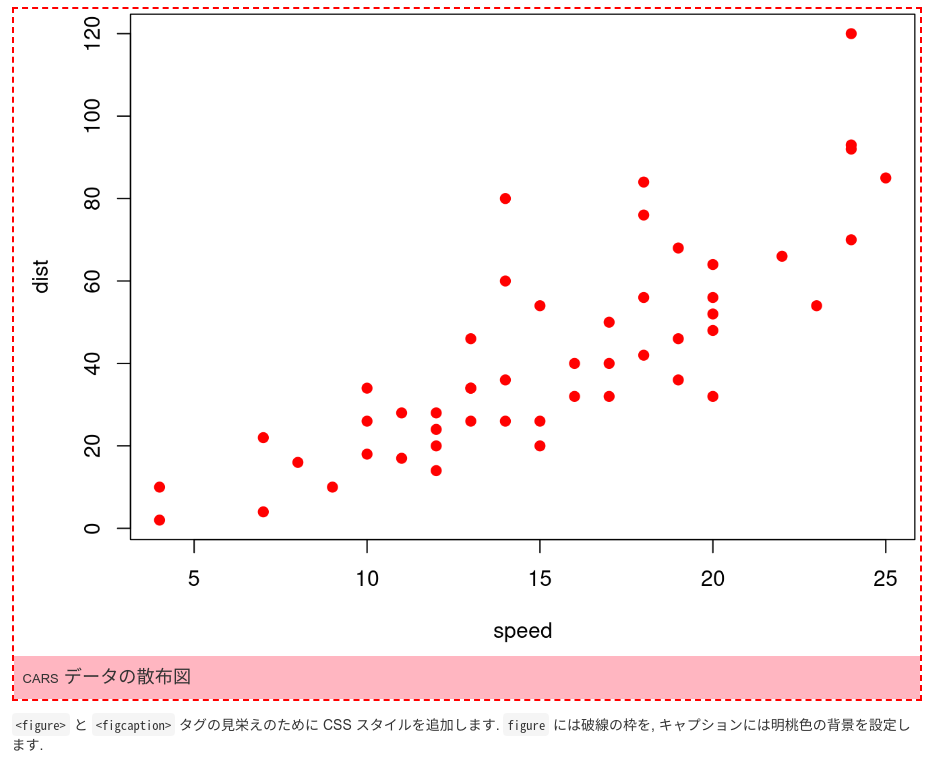
\includegraphics[width=1\linewidth,height=1\textheight,keepaspectratio]{JP/images/hook-html5} 

}

\caption{HTML5 figure タグ内の図}\label{fig:hook-html5}
\end{figure}

この例はファイルパス \texttt{x} と \texttt{plot} フック\index{出力フック!plot}の活用の可能性を示すものです. 図のスタイルのカスタマイズが必要なだけなら, HTML5 タグを使わなくてもよいです. たいていの場合, デフォルトの \texttt{plot} フックはこのような HTML コードに画像を出力します.

\begin{Shaded}
\begin{Highlighting}[]
\KeywordTok{\textless{}div}\OtherTok{ class=}\StringTok{"figure"}\KeywordTok{\textgreater{}}
  \KeywordTok{\textless{}img}\OtherTok{ src=}\StringTok{"ファイルパス"} \KeywordTok{/\textgreater{}}
  \KeywordTok{\textless{}p}\OtherTok{ class=}\StringTok{"caption"}\KeywordTok{\textgreater{}}\NormalTok{キャプション}\KeywordTok{\textless{}/p\textgreater{}}
\KeywordTok{\textless{}/div\textgreater{}}
\end{Highlighting}
\end{Shaded}

よって \texttt{div.figure} と \texttt{p.caption} に対して CSS ルールを定義するだけで可能となります.

\hypertarget{chunk-hooks}{%
\chapter{チャンクフック (*)}\label{chunk-hooks}}

チャンクフック\index{チャンクフック}\index{chunk hook|see{チャンクフック}}はあるチャンクオプションの値が \texttt{NULL} ではないことが引き金となる関数です. チャンクフックはチャンク内でのコードの実行の範囲を越えて追加のタスクを実行する方法を提供します. 例えばグラフに後処理をしたいときがあるかもしれません (例えば\ref{crop-plot}, \ref{optipng}節) し, コードチャンクの実行時間を記録したいかもしれません. このようなタスクはレポート内の計算や分析に必須ではないかもしれませんが, 例えばグラフを改良したり最も時間のかかっているチャンクを特定したりといった, 他の目的に対しては有用になりえます.

例えばコンソールになんらかの情報を表示したりというように, チャンクフックを純粋に副作用のために使うことができますし, あるいは返り値が文字列であれば, 出力文書にこの値を書き出すように作ることもできます.

出力フック (\ref{output-hooks}章参照)のように, チャンクフックは \texttt{knitr::knit\_hooks}\index{knitr!knit\_hooks} オブジェクトにて登録されます. 出力フックの名前は \textbf{knitr} によって予約されているので, カスタムチャンクフックに使ってはならないことに注意してください.

\begin{Shaded}
\begin{Highlighting}[numbers=left,,]
\FunctionTok{names}\NormalTok{(knitr}\SpecialCharTok{:::}\NormalTok{.default.hooks)}
\end{Highlighting}
\end{Shaded}

\begin{verbatim}
##  [1] "source"          "output"         
##  [3] "warning"         "message"        
##  [5] "error"           "plot"           
##  [7] "inline"          "chunk"          
##  [9] "text"            "evaluate.inline"
## [11] "evaluate"        "document"
\end{verbatim}

チャンクフックは同じ名前のチャンクオプション\index{チャンクオプション!チャンクフック|see {チャンクフック}}と関連付けられています. 例えば \texttt{greet} という名前のチャンクフックを登録できます.

\begin{Shaded}
\begin{Highlighting}[numbers=left,,]
\NormalTok{knitr}\SpecialCharTok{::}\NormalTok{knit\_hooks}\SpecialCharTok{$}\FunctionTok{set}\NormalTok{(}\AttributeTok{greet =} \ControlFlowTok{function}\NormalTok{(before) \{}
  \ControlFlowTok{if}\NormalTok{ (before) }
    \StringTok{"Hello!"} \ControlFlowTok{else} \StringTok{"Bye!"}
\NormalTok{\})}
\end{Highlighting}
\end{Shaded}

この後すぐにフック関数の引数について説明します. まずは以下のチャンクでチャンクオプション \texttt{greet = TRUE} を設定してみます.

\begin{Shaded}
\begin{Highlighting}[]
\InformationTok{\textasciigrave{}\textasciigrave{}\textasciigrave{}\{r, greet=TRUE\}}
\InformationTok{1 + 1}
\InformationTok{\textasciigrave{}\textasciigrave{}\textasciigrave{}}
\end{Highlighting}
\end{Shaded}

するとチャンクの前に ``Hello!'' という文字が現れ, 以下のチャンクの出力部の後に ``Bye!'' という文字が現れます. これは両者が文字列だからです.

\begin{quote}
Hello!

\begin{Shaded}
\begin{Highlighting}[numbers=left,,]
\DecValTok{1} \SpecialCharTok{+} \DecValTok{1}
\end{Highlighting}
\end{Shaded}

\begin{verbatim}
## [1] 2
\end{verbatim}

Bye!
\end{quote}

チャンクフック関数は \texttt{before} ・ \texttt{options} ・ \texttt{envir} ・ \texttt{name} の4つの引数を取ることができます. 言い換えるならこのような形式にすることができます.

\begin{Shaded}
\begin{Highlighting}[]
\ControlFlowTok{function}\NormalTok{(before, options, envir, name) \{}

\NormalTok{\}}
\end{Highlighting}
\end{Shaded}

4つの引数はすべて任意です. 4, 3, 2, 1つ, あるいは引数がなくとも可能です. 上記の例では \texttt{before} 引数1つだけを使っています. これらの引数の意味はこのようなものです.

\begin{itemize}
\item
  \texttt{before}: チャンクフックが現在, 実行される前か後かです. チャンクフックはコードチャンクごとに2度実行される, つまり直前に1度 \texttt{hook(before = TRUE)} が, 直後に \texttt{hook(before = FALSE)} が実行されることに注意してください.
\item
  \texttt{options}: 現在のコードチャンクのチャンクオプションのリストです. 例えば \texttt{list(fig.width = 5, echo = FALSE, ...)} のような値です.
\item
  \texttt{envir}: チャンクフックが評価される環境です.
\item
  \texttt{name}: チャンクフックのトリガーとなるチャンクオプションの名前です.
\end{itemize}

この章の冒頭で言及したように, チャンクフックの返す値で文字列でないものは無視され, 文字列は出力文書に書き出されます.

\hypertarget{crop-plot}{%
\section{グラフをクロップする}\label{crop-plot}}

チャンクフック\texttt{knitr::hook\_pdfcrop()}\index{knitr!hook\_pdfcrop()}\index{チャンクフック!グラフのクロップ} は PDF やその他の種類の画像ファイルをクロップするのに使うことができます. つまりグラフから余分な余白を削除します. これを有効にするには, コードチャンク内で \texttt{knit\_hooks\$set()}\index{knitr!knit\_hooks} を使って設定し, 対応するチャンクオプションをオンにしてください. これが例です.

\begin{Shaded}
\begin{Highlighting}[numbers=left,,]
\NormalTok{knitr}\SpecialCharTok{::}\NormalTok{knit\_hooks}\SpecialCharTok{$}\FunctionTok{set}\NormalTok{(}\AttributeTok{crop =}\NormalTok{ knitr}\SpecialCharTok{::}\NormalTok{hook\_pdfcrop)}
\end{Highlighting}
\end{Shaded}

それからグラフをクロップするコードチャンクで, チャンクオプション \texttt{crop = TRUE}\index{チャンクオプション!crop} を使うことができます.

フック関数 \texttt{hook\_pdfcrop()} は PDF ファイルをクロップするために内部プログラム \texttt{pdfcrop} を呼び出します. このプログラムはよく LaTeX の配布パッケージに同梱されています (例えば TeX Live や MikTeX). あなたのシステムでこれが使用可能かはこのようにして確認できます.

\begin{Shaded}
\begin{Highlighting}[numbers=left,,]
\CommentTok{\# 返り値が空でないなら使用可能}
\FunctionTok{Sys.which}\NormalTok{(}\StringTok{"pdfcrop"}\NormalTok{)}
\end{Highlighting}
\end{Shaded}

\begin{verbatim}
##                  pdfcrop 
## "/usr/local/bin/pdfcrop"
\end{verbatim}

LaTeX 配布パッケージの TinyTeX (\ref{install-latex}節参照) を使っていて, なおかつ \texttt{pdfcrop} があなたのシステムで利用できないなら, \texttt{tinytex::tlmgr\_install(\textquotesingle{}pdfcrop\textquotesingle{})}\index{tinytex!tlmgr\_install()} でインストールすることもできます.

PNG や JPEG といった PDF でないグラフ画像ファイルに対しては, このフック関数は R パッケージの \textbf{magick} \autocite{R-magick}\index{R パッケージ!magick}を呼び出してクロップします. この R パッケージがインストールされているか確認する必要があります. 図\ref{fig:crop-no}はクロップされていないグラフで, 図 \ref{fig:crop-yes}はクロップされた同じグラフです.

\begin{figure}

{\centering \framebox{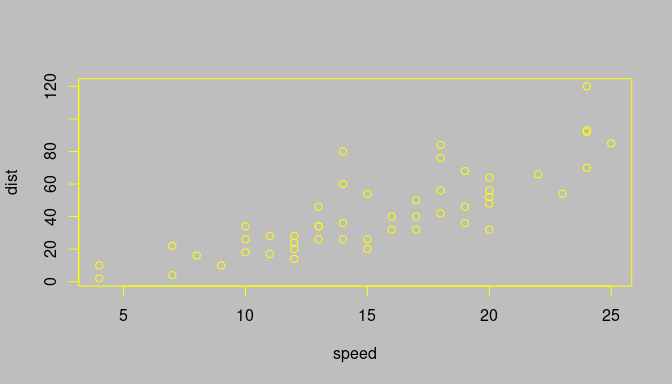
\includegraphics[width=1\linewidth,height=1\textheight,]{rmarkdown-cookbook_files/figure-latex/crop-no-1} } 

}

\caption{クロップされていないグラフ}\label{fig:crop-no}
\end{figure}

\begin{figure}

{\centering \framebox{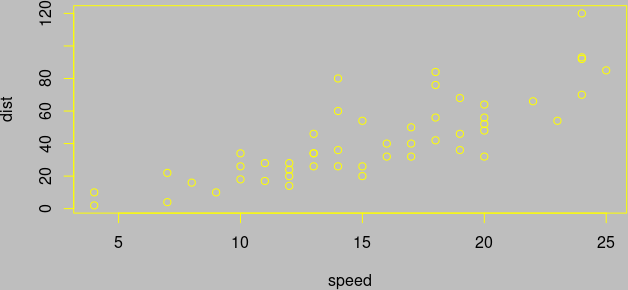
\includegraphics[width=1\linewidth,height=1\textheight,]{rmarkdown-cookbook_files/figure-latex/crop-yes-1} } 

}

\caption{クロップされたグラフ}\label{fig:crop-yes}
\end{figure}

\hypertarget{optipng}{%
\section{PNG のグラフを最適化する}\label{optipng}}

OptiPNG (\url{http://optipng.sourceforge.net})\index{OptiPNG} プログラムをインストールしているなら, PNG 形式のグラフ画像ファイルを画質を劣化させることなく縮小するために最適化するのに使うこともできます\index{チャンクフック!PNG の最適化}\index{図!PNG の最適化}.

\begin{Shaded}
\begin{Highlighting}[numbers=left,,]
\NormalTok{knitr}\SpecialCharTok{::}\NormalTok{knit\_hooks}\SpecialCharTok{$}\FunctionTok{set}\NormalTok{(}\AttributeTok{optipng =}\NormalTok{ knitr}\SpecialCharTok{::}\NormalTok{hook\_optipng)}
\end{Highlighting}
\end{Shaded}

このフックを設定した後で, OPtiPNG へのコマンドライン引数を通すのにチャンクオプション \texttt{optipng}\index{チャンクオプション!optipng}を使うことができます (例えば \texttt{optipng = \textquotesingle{}-o7\textquotesingle{}}). コマンドライン引数はオプションなので, フックを有効にするために \texttt{optipng = \textquotesingle{}\textquotesingle{}} とだけ書くことも可能です. 使用可能な引数を知るには OptiPNG のウェブサイト上にあるユーザーマニュアルを見てください.

macOS ユーザーは Homebrew (\url{https://brew.sh}) で簡単に OptiPNG をインストールできます (\texttt{brew install optipng}).

\hypertarget{time-chunk}{%
\section{チャンクの実行時間をレポートする}\label{time-chunk}}

\textbf{knitr} はデフォルトでは knit 処理中にテキストベースの進捗バーを提供します. より正確なチャンクの時間の情報がほしいなら, 各チャンクの時間を記録するカスタムチャンクフックを登録することもできます. これはそのようなフックの例です.

\begin{Shaded}
\begin{Highlighting}[numbers=left,,]
\NormalTok{knitr}\SpecialCharTok{::}\NormalTok{knit\_hooks}\SpecialCharTok{$}\FunctionTok{set}\NormalTok{(}\AttributeTok{time\_it =} \FunctionTok{local}\NormalTok{(\{}
\NormalTok{  now }\OtherTok{\textless{}{-}} \ConstantTok{NULL}
  \ControlFlowTok{function}\NormalTok{(before, options) \{}
    \ControlFlowTok{if}\NormalTok{ (before) \{}
      \CommentTok{\# 各チャンクの直前の時刻を記録する}
\NormalTok{      now }\OtherTok{\textless{}\textless{}{-}} \FunctionTok{Sys.time}\NormalTok{()}
\NormalTok{    \} }\ControlFlowTok{else}\NormalTok{ \{}
      \CommentTok{\# チャンク直後の時刻との差を計算する}
\NormalTok{      res }\OtherTok{\textless{}{-}} \FunctionTok{difftime}\NormalTok{(}\FunctionTok{Sys.time}\NormalTok{(), now)}
      \CommentTok{\# 時間を表示するための文字列を返す}
      \FunctionTok{paste}\NormalTok{(}\StringTok{"Time for this code chunk to run:"}\NormalTok{, res)}
\NormalTok{    \}}
\NormalTok{  \}}
\NormalTok{\}))}
\end{Highlighting}
\end{Shaded}

これ以降, チャンクオプション \texttt{time\_it} をチャンクに使うことができます. これが例です.

\begin{verbatim}
```{r, time_it = TRUE}
Sys.sleep(2)
```
\end{verbatim}

全てのコードチャンクで時間を表示したいなら, もちろん \texttt{knitr::opts\_chunk\$set(time\_it = TRUE)} でグローバルに設定することができます.

上記のフック関数で, チャンクオプションのより詳細な情報を出力することもできます. つまりフック関数の \texttt{options} 引数を使います. 例えば, 返り値にチャンクラベルを表示する手もあります.

\begin{Shaded}
\begin{Highlighting}[numbers=left,,]
\FunctionTok{paste}\NormalTok{(}\StringTok{"Time for the chunk"}\NormalTok{, options}\SpecialCharTok{$}\NormalTok{label, }\StringTok{"to run:"}\NormalTok{, res)}
\end{Highlighting}
\end{Shaded}

あるいはフック関数で表示させずに記録するという手もあります.

\begin{Shaded}
\begin{Highlighting}[numbers=left,,]
\NormalTok{all\_times }\OtherTok{\textless{}{-}} \FunctionTok{list}\NormalTok{()  }\CommentTok{\# 全てのチャンクの時間を保存する}
\NormalTok{knitr}\SpecialCharTok{::}\NormalTok{knit\_hooks}\SpecialCharTok{$}\FunctionTok{set}\NormalTok{(}\AttributeTok{time\_it =} \FunctionTok{local}\NormalTok{(\{}
\NormalTok{  now }\OtherTok{\textless{}{-}} \ConstantTok{NULL}
  \ControlFlowTok{function}\NormalTok{(before, options) \{}
    \ControlFlowTok{if}\NormalTok{ (before) \{}
\NormalTok{      now }\OtherTok{\textless{}\textless{}{-}} \FunctionTok{Sys.time}\NormalTok{()}
\NormalTok{    \} }\ControlFlowTok{else}\NormalTok{ \{}
\NormalTok{      res }\OtherTok{\textless{}{-}} \FunctionTok{difftime}\NormalTok{(}\FunctionTok{Sys.time}\NormalTok{(), now)}
\NormalTok{      all\_times[[options}\SpecialCharTok{$}\NormalTok{label]] }\OtherTok{\textless{}\textless{}{-}}\NormalTok{ res}
\NormalTok{    \}}
\NormalTok{  \}}
\NormalTok{\}))}
\end{Highlighting}
\end{Shaded}

すると \texttt{all\_times} オブジェクトで全ての実行時間情報にアクセスすることができます. このオブジェクトはチャンクラベルを名前にもつ名前つきリストで, 各要素の値はそれぞれのチャンクの実行時間です.

最後に技術的な注意事項として, 先ほどのフックで使われた \texttt{local()} 関数に詳しくない人もいるかもしれませんので, これについて説明したいとおもいます. この関数でコードを「ローカルな」環境で実行することができます. その主な恩恵は, コード内で作られた変数はこの環境内のローカルなものになるので, 外部の環境, たいていの場合はグローバル環境を汚染することがないということです. 例えばここでは \texttt{local()} 内で \texttt{now} 変数を作成し, これを \texttt{time\_it} 内で使用しています. フック関数内では通常の代入演算子 \texttt{\textless{}-} の代わりに二重アロー演算子 \texttt{\textless{}\textless{}-} で \texttt{now} の値を更新しています. \texttt{\textless{}\textless{}-} が親環境, この場合は \texttt{local()} 環境の変数に代入し, そして \texttt{\textless{}-} は単に現在の環境にのみ値を代入するというのが理由です. 各コードチャンクが評価される直前に, ローカル変数 \texttt{now} は現在の時刻を記録します. \texttt{local()} は与えられたコード内の最後の値を返し, それはここでは フック関数であることに注意してください. 簡潔に言うなら, \texttt{local()} は, ローカルでのみ使われ グローバル環境で使われない変数を露出しないことで, ワークスペースの掃除機となれるということです. グローバル環境に変数 \texttt{now} が作られることが気にならないのならば, \texttt{local()} を使わないという選択をすることもできます.

\hypertarget{show-header}{%
\section{出力にチャンクヘッダを表示する}\label{show-header}}

読者に元のチャンクヘッダのコードを表示したい時もあるかもしれません. 例えば R Markdown のチュートリアルを書いていて, チャンクの出力とその出力を生成するのに使用したチャンクオプションの両方を表示したいことがあるかもしれません. よって読者が自分で同じことをする方法を学ぶことができるというわけです.

本来のチャンクオプションは実際にはチャンクオプションの \texttt{params.scr} 内に文字列として保存されています. これを知ったあなたは \texttt{params.src} を出力するチャンクフックを書くこともできます. 以下はその完全な例です.

\begin{Shaded}
\begin{Highlighting}[]
\CommentTok{{-}{-}{-}}
\AnnotationTok{title:}\CommentTok{ 出力にチャンクヘッダを表示する}
\CommentTok{{-}{-}{-}}

\NormalTok{本来のチャンクヘッダとフッタの内側にチャンクを出力する}
\InformationTok{\textasciigrave{}wrapper\textasciigrave{}}\NormalTok{ という名前のチャンクフックを用意します.}

\InformationTok{\textasciigrave{}\textasciigrave{}\textasciigrave{}\{r, setup, include=FALSE\}}
\InformationTok{knitr::knit\_hooks$set(wrapper = function(before, options) \{}
\InformationTok{  \# 本来のチャンクはインデントされる}
\InformationTok{  if (is.null(indent \textless{}{-} options$indent)) indent \textless{}{-} \textquotesingle{}\textquotesingle{}}
\InformationTok{  }
\InformationTok{  \# wrapper=TRUE オプションを隠す}
\InformationTok{  opts \textless{}{-} gsub(\textquotesingle{}, wrapper=TRUE\textquotesingle{}, \textquotesingle{}\textquotesingle{}, options$params.src)}
\InformationTok{  }
\InformationTok{  if (before) \{}
\InformationTok{    \# ヘッダを追加する}
\InformationTok{    sprintf(\textquotesingle{}\textbackslash{}n\textbackslash{}n\%s\textasciigrave{}\textasciigrave{}\textasciigrave{}\textasciigrave{}\textbackslash{}n\textasciigrave{}\textasciigrave{}\textasciigrave{}\{r,\%s\}\textbackslash{}n\textasciigrave{}\textasciigrave{}\textasciigrave{}\textasciigrave{}\textbackslash{}n\textquotesingle{}, indent, opts)}
\InformationTok{  \} else \{}
\InformationTok{    \# フッタを追加する}
\InformationTok{    sprintf(\textquotesingle{}\textbackslash{}n\textbackslash{}n\%s\textasciigrave{}\textasciigrave{}\textasciigrave{}\textasciigrave{}\textbackslash{}n\textasciigrave{}\textasciigrave{}\textasciigrave{}\textbackslash{}n\textasciigrave{}\textasciigrave{}\textasciigrave{}\textasciigrave{}\textbackslash{}n\textquotesingle{}, indent)}
\InformationTok{  \}}
\InformationTok{\})}
\InformationTok{\textasciigrave{}\textasciigrave{}\textasciigrave{}}

\NormalTok{ここでチャンクオプション }\InformationTok{\textasciigrave{}wrapper=TRUE\textasciigrave{}}\NormalTok{  でフックを適用します. }\InformationTok{\textasciigrave{}wrapper=TRUE\textasciigrave{}}\NormalTok{ をヘッダの最後に置くことと, 正確に }\InformationTok{\textasciigrave{}wrapper=TRUE\textasciigrave{}}\NormalTok{ でなければならず, 上記で呼び出されている }\InformationTok{\textasciigrave{}gsub()\textasciigrave{}}\NormalTok{ を修正しない限り, 例えば }\InformationTok{\textasciigrave{}wrapper=T\textasciigrave{}}\NormalTok{ はダメで,  コンマとスペースの後に続けなければならないことも忘れないでください.}

\InformationTok{\textasciigrave{}\textasciigrave{}\textasciigrave{}\{r, test{-}label, collapse=TRUE, wrapper=TRUE\}}
\InformationTok{1 + 1}
\InformationTok{plot(cars)}
\InformationTok{\textasciigrave{}\textasciigrave{}\textasciigrave{}}

\NormalTok{本来のチャンクヘッダが出力に現れるはずです. フックはチャンクがインデントされていても動作するはずです. これが例です.}

\SpecialStringTok{{-} }\NormalTok{箇条書きその1}

  \InformationTok{\textasciigrave{}\textasciigrave{}\textasciigrave{}\{r, eval=TRUE, wrapper=TRUE\}}
\InformationTok{  2 + 2}
\InformationTok{  \textasciigrave{}\textasciigrave{}\textasciigrave{}}

\SpecialStringTok{{-} }\NormalTok{もう1つ箇条書き}
\end{Highlighting}
\end{Shaded}

基本的に, \texttt{\textasciigrave{}\textasciigrave{}\textasciigrave{}\{r,\ \}} 内に \texttt{options\$params.src} から取り出したチャンクヘッダ入れることで元のヘッダを再現しています. そこでこの行を1組の4連続バッククオートで囲んでいるので, 出力時にはそのまま表示されます. 本来のコードチャンクはインデントされるかもしれない (例: 箇条書き内にネストされている場合), 適切にインデントを追加することも必要になります. これはチャンクオプション \texttt{options\$indent} に保存されています.

上記の例の最後の, 箇条書き内の出力はこのようになります.

\begin{quote}
\begin{itemize}
\item
  箇条書きその1

\begin{verbatim}
```{r, eval=TRUE}
\end{verbatim}

\begin{Shaded}
\begin{Highlighting}[]
\DecValTok{2} \SpecialCharTok{+} \DecValTok{2}
\end{Highlighting}
\end{Shaded}

\begin{verbatim}
## [1] 4
\end{verbatim}

\begin{verbatim}
```
\end{verbatim}
\item
  もう1つ箇条書き
\end{itemize}
\end{quote}

コードチャンクが評価され, チャンクヘッダも追加されていることが分かったかと思います.

\hypertarget{rgl-3d}{%
\section{rgl によるインタラクティブな3次元グラフを埋め込む}\label{rgl-3d}}

\textbf{rgl} パッケージ \autocite{R-rgl}\index{R パッケージ!rgl} はインタラクティブな3次元グラフを生成するのに使うことができます. WebGL 形式\index{WebGL}で保存されているなら, これらのグラフはインタラクティブになります. これはフック関数 \texttt{rgl::hook\_webgl()}\index{チャンクフック!WebGL グラフ}\index{図!WebGL} を使うことで可能になります. 以下の例は \textbf{rgl} と \textbf{knitr} で 3次元グラフをインタラクティブ性を保ったまま保存できるようにする方法を示しています.

\begin{Shaded}
\begin{Highlighting}[]
\CommentTok{{-}{-}{-}}
\AnnotationTok{title:}\CommentTok{ rgl で3次元グラフを埋め込む}
\AnnotationTok{output:}\CommentTok{ html\_document}
\CommentTok{{-}{-}{-}}

\NormalTok{**rgl** を保存するフック関数を用意する.}

\InformationTok{\textasciigrave{}\textasciigrave{}\textasciigrave{}\{r, setup\}}
\InformationTok{library(rgl)}
\InformationTok{knitr::knit\_hooks$set(webgl = hook\_webgl)}
\InformationTok{\textasciigrave{}\textasciigrave{}\textasciigrave{}}

\NormalTok{フックを有効にした後で, チャンクオプション }\InformationTok{\textasciigrave{}webgl = TRUE\textasciigrave{}}\NormalTok{ で}
\NormalTok{この3次元グラフが動作するかを確認してください.}

\InformationTok{\textasciigrave{}\textasciigrave{}\textasciigrave{}\{r, test{-}rgl, webgl=TRUE\}}
\InformationTok{x \textless{}{-} sort(rnorm(1000))}
\InformationTok{y \textless{}{-} rnorm(1000)}
\InformationTok{z \textless{}{-} rnorm(1000) + atan2(x,y)}
\InformationTok{plot3d(x, y, z, col = rainbow(1000))}
\InformationTok{\textasciigrave{}\textasciigrave{}\textasciigrave{}}
\end{Highlighting}
\end{Shaded}

この例をコンパイルすると図\ref{fig:rgl-3d}のようなインタラクティブな3次元散布図が得られるはずです. インタラクティブなグラフは出力フォーマットが HTML の時にのみ動作することに注意してください.

\begin{figure}

{\centering 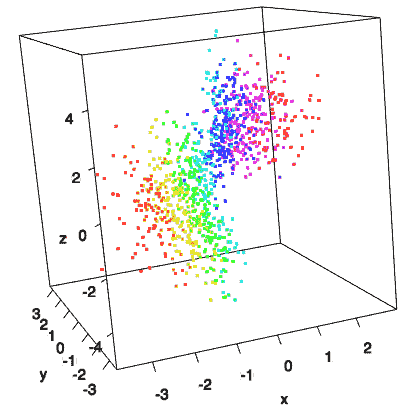
\includegraphics[width=1\linewidth,height=1\textheight,keepaspectratio]{JP/images/rgl-3d} 

}

\caption{rgl パッケージから生成した3次元散布図}\label{fig:rgl-3d}
\end{figure}

\hypertarget{knitr-misc}{%
\chapter{その他の knitr のトリック}\label{knitr-misc}}

チャンクオプション(\ref{chunk-options}章)・出力フック(\ref{output-hooks}章)・チャンクフック ( \ref{chunk-hooks}章) にとどまらず, 他にも役に立つ関数やトリックが \textbf{knitr}\index{knitr}にはあります. この章では, コードチャンクの再利用, knit の早期終了, グラフの配置場所のカスタマイズの方法などといったトリックを紹介します.

\hypertarget{reuse-chunks}{%
\section{コードチャンクを再利用する}\label{reuse-chunks}}

コードチャンク\index{コードチャンク}の再利用は, コピーアンドペーストなしで文書のどの場所でも自由にすることができます. ポイントはコードチャンクにラベルを付けることで, そうすると他の場所でラベルによって参照することができます. コードチャンクの再利用\index{コードチャンク!再利用}には3種類の方法があります.

\hypertarget{embed-chunk}{%
\subsection{チャンクを別の場所にも埋め込む (*)}\label{embed-chunk}}

あるコードチャンクを別の場所で, そのラベルを \texttt{\textless{}\textless{}\textgreater{}\textgreater{}}\index{コードチャンク!埋め込み}\index{コードチャンク!<<>>} で囲むことで埋め込めます. すると \textbf{knitr} は自動的に \texttt{\textless{}\textless{}ラベル\textgreater{}\textgreater{}} を実際のコードへと展開してくれます. 例えば, この方法で R 関数を作ることができます.

\begin{Shaded}
\begin{Highlighting}[]
\NormalTok{華氏温度を摂氏温度に変換する関数を定義する}

\InformationTok{\textasciigrave{}\textasciigrave{}\textasciigrave{}\{r, f2c\}}
\InformationTok{F2C \textless{}{-} function(x) \{}
\InformationTok{  \textless{}\textless{}check{-}arg\textgreater{}\textgreater{}}
\InformationTok{  \textless{}\textless{}convert\textgreater{}\textgreater{}}
\InformationTok{\}}
\InformationTok{\textasciigrave{}\textasciigrave{}\textasciigrave{}}

\NormalTok{最初に入力値が数値か確認する}

\InformationTok{\textasciigrave{}\textasciigrave{}\textasciigrave{}\{r, check{-}arg, eval=FALSE\}}
\InformationTok{  if (!is.numeric(x)) stop("入力は数値でなければなりません!")}
\InformationTok{\textasciigrave{}\textasciigrave{}\textasciigrave{}}

\NormalTok{それから実際に変換します}

\InformationTok{\textasciigrave{}\textasciigrave{}\textasciigrave{}\{r, convert, eval=FALSE\}}
\InformationTok{  (x {-} 32) * 5/ 9}
\InformationTok{\textasciigrave{}\textasciigrave{}\textasciigrave{}}
\end{Highlighting}
\end{Shaded}

これはドナルド=クヌースの提案する\href{https://en.wikipedia.org/wiki/Literate_programming}{文芸プログラミング} の主要なアイディアの1つに基づいたものです. この技術の利点は (複雑な) コードを小さな部品に分割し, 別々のコードチャンクに書き, 文脈の中で説明することができる点です. 全ての部品は実行される主要なコードチャンクで構成することができます.

上記の例に対して, \texttt{f2c} というラベルのある最初のコードチャンクはこうなります.

\begin{Shaded}
\begin{Highlighting}[]
\InformationTok{\textasciigrave{}\textasciigrave{}\textasciigrave{}\{r, f2c\}}
\InformationTok{F2C \textless{}{-} function(x) \{}
\InformationTok{  if (!is.numeric(x)) stop("The input must be numeric!")}
\InformationTok{  (x {-} 32) * 5/ 9}
\InformationTok{\}}
\InformationTok{\textasciigrave{}\textasciigrave{}\textasciigrave{}}
\end{Highlighting}
\end{Shaded}

1つのコードチャンクに好きな数のコードチャンクを埋め込むことが可能です. 埋め込みは再帰的にすることも可能です. 例えば, チャンク A をチャンク B に埋め込み, さらにチャンク B をチャンク C に埋め込むこともできます. チャンク C はチャンク B から読み込まれたチャンク A を含むことになります.

マーカー \texttt{\textless{}\textless{}ラベル\textgreater{}\textgreater{}} は独立した行に置く必要はありません. コードチャンクのどこにでも埋め込むことができます.

\hypertarget{same-label}{%
\subsection{別のチャンクで同一のチャンクラベルを使う}\label{same-label}}

完全に同じコードを2回異常使いたいならば, ラベル付きのチャンクを定義し, そして同じラベルであるものの中身が空のチャンクを作ることもできます. 例えばこのように.

\begin{Shaded}
\begin{Highlighting}[]
\NormalTok{これは評価されないコードチャンクです}

\InformationTok{\textasciigrave{}\textasciigrave{}\textasciigrave{}\{r, chunk{-}one, eval=FALSE\}}
\InformationTok{1 + 1}
\InformationTok{2 + 2}
\InformationTok{\textasciigrave{}\textasciigrave{}\textasciigrave{}}

\NormalTok{実際に評価されるのはここです}

\InformationTok{\textasciigrave{}\textasciigrave{}\textasciigrave{}\{r, chunk{-}one, eval=TRUE\}}
\InformationTok{\textasciigrave{}\textasciigrave{}\textasciigrave{}}
\end{Highlighting}
\end{Shaded}

上記の例でチャンクラベル ``chunk-one'' を2度使い, 2度目のチャンクは最初のチャンクの単なる再利用です.

グラフかあるいは他のファイルを生成するのに, この方法で複数回コードチャンクを実行するのはお薦めしません. 最後のチャンクで作成された画像ファイルがそれ以前のものを上書きするかもしれないからです. これらのチャンクのうち1つだけにチャンクオプション \texttt{eval = TRUE} を使い, それ以外では \texttt{eval =FALSE} を使うのならば大丈夫です.

\hypertarget{ref-label}{%
\subsection{参照ラベルを使う (*)}\label{ref-label}}

チャンクオプション \texttt{ref.label}\index{チャンクオプション!ref.label} はチャンクの中身を取得するために, そのチャンクラベルのベクトルを取ります. 例えば以下の \texttt{chunk-a} というラベルのコードチャンクは \texttt{chunk-c} と \texttt{chunk-b} を結合したものです.

\begin{Shaded}
\begin{Highlighting}[]
\InformationTok{\textasciigrave{}\textasciigrave{}\textasciigrave{}\{r chunk{-}a, ref.label=c(\textquotesingle{}chunk{-}c\textquotesingle{}, \textquotesingle{}chunk{-}b\textquotesingle{})\}}
\InformationTok{\textasciigrave{}\textasciigrave{}\textasciigrave{}}

\InformationTok{\textasciigrave{}\textasciigrave{}\textasciigrave{}\{r chunk{-}b\}}
\InformationTok{\# これはチャンク b}
\InformationTok{1 + 1}
\InformationTok{\textasciigrave{}\textasciigrave{}\textasciigrave{}}

\InformationTok{\textasciigrave{}\textasciigrave{}\textasciigrave{}\{r chunk{-}c\}}
\InformationTok{\# これはチャンク c}
\InformationTok{2 + 2}
\InformationTok{\textasciigrave{}\textasciigrave{}\textasciigrave{}}
\end{Highlighting}
\end{Shaded}

言い換えるなら, \texttt{chunk-a} は本質的にこうなります.

\begin{Shaded}
\begin{Highlighting}[]
\InformationTok{\textasciigrave{}\textasciigrave{}\textasciigrave{}\{r chunk{-}a\}}
\InformationTok{\# これはチャンク c}
\InformationTok{2 + 2}
\InformationTok{\# これはチャンク b}
\InformationTok{1 + 1}
\InformationTok{\textasciigrave{}\textasciigrave{}\textasciigrave{}}
\end{Highlighting}
\end{Shaded}

チャンクオプション \texttt{ref.label} は, コピーアンドペーストを使うことなくコードチャンクを再構成する, とても柔軟な方法を提供しています. 参照先のコードチャンクが \texttt{ref.label} が使われたチャンクの前にあるか, 後にあるかは問題になりません. 先に書かれたコードチャンクは後のコードチャンクを参照できます.

\ref{code-appendix}節にはこのチャンクオプションの応用例があります.

\hypertarget{load-cache}{%
\section{オブジェクトが作られる前に使用する (*)}\label{load-cache}}

コードチャンクとインライン R コードを含む \textbf{knitr} 文書内の全てのコードは, 始点から終点まで順番に実行されます. 理論上は, 値が代入される前の変数を使うことができません. しかしいくつかの場合では, 文書内で変数の値により早く言及したいことがあるかもしれません. 例えば結果を論文の概要に掲載したいというのはよくある状況ですが, 結果は実際には文書のもっと後で計算されます. 以下の例はそのアイディアを具体化したものですが, 実行はできません.

\begin{Shaded}
\begin{Highlighting}[]
\CommentTok{{-}{-}{-}}
\AnnotationTok{title:}\CommentTok{ 重要なレポート}
\CommentTok{概要: \textgreater{}}
\CommentTok{  この分析では \textasciigrave{}x\textasciigrave{} の平均値が}
\CommentTok{  \textasciigrave{}r mx\textasciigrave{} であった.}
\CommentTok{{-}{-}{-}}

\NormalTok{我々は次のチャンクで }\InformationTok{\textasciigrave{}mx\textasciigrave{}}\NormalTok{ を作成した.}

\InformationTok{\textasciigrave{}\textasciigrave{}\textasciigrave{}\{r\}}
\InformationTok{x \textless{}{-} 1:100}
\InformationTok{mx \textless{}{-} mean(x)}
\InformationTok{\textasciigrave{}\textasciigrave{}\textasciigrave{}}
\end{Highlighting}
\end{Shaded}

この問題を解決するには, オブジェクトの値がどこかに保存され, 文書が次回コンパイルされる時に読み込まれなければなりません. これは, 文書が最低でも2回コンパイルされなければならないという意味であることに注意してください. 以下は \texttt{saveRDS()} 関数を使った, 実行可能な解決策の1つです.

\begin{Shaded}
\begin{Highlighting}[]
\InformationTok{\textasciigrave{}\textasciigrave{}\textasciigrave{}\{r, include=FALSE\}}
\InformationTok{mx \textless{}{-} if (file.exists(\textquotesingle{}mean.rds\textquotesingle{})) \{}
\InformationTok{  readRDS(\textquotesingle{}mean.rds\textquotesingle{})}
\InformationTok{\} else \{}
\InformationTok{  "\textasciigrave{}mx\textasciigrave{} の値はまだ利用できない"}
\InformationTok{\}}
\InformationTok{\textasciigrave{}\textasciigrave{}\textasciigrave{}}

\NormalTok{{-}{-}{-}}
\NormalTok{title: 重要なレポート}
\NormalTok{概要: \textgreater{}}
\NormalTok{  この分析では }\InformationTok{\textasciigrave{}x\textasciigrave{}}\NormalTok{ の平均値が}
  \InformationTok{\textasciigrave{}r mx\textasciigrave{}}\NormalTok{ であった.}
\NormalTok{{-}{-}{-}}

\NormalTok{我々は次のチャンクで }\InformationTok{\textasciigrave{}mx\textasciigrave{}}\NormalTok{ を作成した.}

\InformationTok{\textasciigrave{}\textasciigrave{}\textasciigrave{}\{r\}}
\InformationTok{x \textless{}{-} 1:100}
\InformationTok{mx \textless{}{-} mean(x)}
\InformationTok{saveRDS(mx, \textquotesingle{}mean.rds\textquotesingle{})}
\InformationTok{\textasciigrave{}\textasciigrave{}\textasciigrave{}}
\end{Highlighting}
\end{Shaded}

最初のコンパイルでは, 概要に「\texttt{mx} の値はまだ利用できない」という文言が現れます. その後, もう1度コンパイルすると \texttt{mx} の値が現れます.

\texttt{knitr::load\_cache()}\index{knitr!load\_cache()} 関数はもう1つの解決策で, キャッシュ\index{キャッシュ}済みの特定のコードチャンクからオブジェクトの値を読み込むことが可能になります. このアイディアは上記の例と似ていますが, オブジェクトが自動でキャッシュデータベースに保存されるため, オブジェクトを手動で保存して読み込む手間を省くことになります. あなたがする必要があるのは \texttt{load\_cache()} で読み込むことだけになります. 以下は単純化した例です.

\begin{Shaded}
\begin{Highlighting}[]
\CommentTok{{-}{-}{-}}
\AnnotationTok{title:}\CommentTok{ An important report}
\AnnotationTok{abstract:}\CommentTok{ \textgreater{}}
\CommentTok{  この分析では \textasciigrave{}x\textasciigrave{} の平均値が}
\CommentTok{  \textasciigrave{}r knitr::load\_cache(\textquotesingle{}mean{-}x\textquotesingle{}, \textquotesingle{}mx\textquotesingle{})\textasciigrave{} であった.}
\CommentTok{{-}{-}{-}}

\NormalTok{我々は次のチャンクで }\InformationTok{\textasciigrave{}mx\textasciigrave{}}\NormalTok{ を作成した.}

\InformationTok{\textasciigrave{}\textasciigrave{}\textasciigrave{}\{r mean{-}x, cache=TRUE\}}
\InformationTok{x \textless{}{-} 1:100}
\InformationTok{mx \textless{}{-} mean(x)}
\InformationTok{\textasciigrave{}\textasciigrave{}\textasciigrave{}}
\end{Highlighting}
\end{Shaded}

この例ではチャンクラベル \texttt{mean-x} をコードチャンクに追加し, これは \texttt{load\_cache()} 関数に与えられています. そしてチャンクオプション \texttt{cache = TRUE}\index{チャンクオプション!cache} でチャンクはキャッシュされています. このコードチャンクの全てのオブジェクトはキャッシュデータベースに保存されます. 繰り返しになりますが, この文書を最低でも2回コンパイルしなければならず. よってオブジェクト \texttt{mx} はキャッシュデータベースから正しく読み込まれます. \texttt{mx} の値が将来も変更される予定がないなら, 文書をこれ以上コンパイルする必要はありません.

もし \texttt{load\_cache()} の第2引数でオブジェクト名を指定しないなら, キャッシュデータベース全体が現在の環境に読み込まれます. 文書の後方でオブジェクトが作成される前に, キャッシュデータベースにあるものならどれでも使うことができます. これが例です.

\begin{Shaded}
\begin{Highlighting}[numbers=left,,]
\NormalTok{knitr}\SpecialCharTok{::}\FunctionTok{load\_cache}\NormalTok{(}\StringTok{"mean{-}x"}\NormalTok{)}
\NormalTok{x  }\CommentTok{\# the object \textasciigrave{}x\textasciigrave{}}
\NormalTok{mx  }\CommentTok{\# the object \textasciigrave{}mx\textasciigrave{}}
\end{Highlighting}
\end{Shaded}

\hypertarget{knit-exit}{%
\section{knit 処理を打ち切る}\label{knit-exit}}

時には knit 処理を文書の末尾よりも早い時点で終了したいかもしれません. 例えば何か分析する作業をしていて, 結果の前半だけを共有したいとか, まだ一番最後のコードが終了していないということがあるかもしれません. このような状況ではコードチャンクで \texttt{knit\_exit()}\index{knitr!knit\_exit()} 関数を使うことができます. この関数はそのチャンクの直後で knit 処理を終わらせることができます.

以下は単純な例です. ここではとても単純なチャンクと, その後にもっと時間のかかるチャンクを配置しています.

\begin{Shaded}
\begin{Highlighting}[]
\InformationTok{\textasciigrave{}\textasciigrave{}\textasciigrave{}\{r\}}
\InformationTok{1 + 1}
\InformationTok{knitr::knit\_exit()}
\InformationTok{\textasciigrave{}\textasciigrave{}\textasciigrave{}}

\NormalTok{あなたは出力のうち上記のコンテンツだけを見たい.}

\InformationTok{\textasciigrave{}\textasciigrave{}\textasciigrave{}\{r\}}
\InformationTok{Sys.sleep(100)}
\InformationTok{\textasciigrave{}\textasciigrave{}\textasciigrave{}}
\end{Highlighting}
\end{Shaded}

通常ならば100秒待たなければなりませんが, \texttt{knit\_exit()} を呼び出しているので文書の残りの部分は無視されます.

\hypertarget{fig-chunk}{%
\section{どこにでもグラフを生成し, 表示させる}\label{fig-chunk}}

グラフは通常コードチャンク内で生成され, その直下に表示されますが, どこに表示するかを好きに指定することも, コードチャンクに隠すこともできます. 以下はその例です.

\begin{Shaded}
\begin{Highlighting}[]
\NormalTok{このコードチャンクでグラフを生成しますが, 表示はしません.}

\InformationTok{\textasciigrave{}\textasciigrave{}\textasciigrave{}\{r cars{-}plot, dev=\textquotesingle{}png\textquotesingle{}, fig.show=\textquotesingle{}hide\textquotesingle{}\}}
\InformationTok{plot(cars)}
\InformationTok{\textasciigrave{}\textasciigrave{}\textasciigrave{}}

\NormalTok{別の段落でグラフを導入します}

\NormalTok{!}\CommentTok{[}\OtherTok{A nice plot.}\CommentTok{]}\NormalTok{(}\InformationTok{\textasciigrave{}r knitr::fig\_chunk(\textquotesingle{}cars{-}plot\textquotesingle{}, \textquotesingle{}png\textquotesingle{})\textasciigrave{}}\NormalTok{)}
\end{Highlighting}
\end{Shaded}

コードチャンクでは, 一時的にグラフを隠すためにチャンクオプション \texttt{fig.show=\textquotesingle{}hide\textquotesingle{}}\index{チャンクオプション!fig.show} を使用しました. それから別の段落でこのグラフ画像のファイルパスを取得するために \texttt{knitr::fig\_chunk()}\index{knitr!fig\_chunk()} 関数を呼び出しました. このパスは普通は \texttt{test\_files/figure-html/cars-plot-1.png} のようになっています. \texttt{fig\_chunk()} 関数にはこのファイルパスを導出するためにチャンクラベルとグラフィックデバイス名を与える必要があります.

\textbf{blogdown} で作成したウェブサイトへの \texttt{fig\_chunk()} の応用を \url{https://stackoverflow.com/a/46305297/559676} で見ることもできます. この関数はどの R Markdown 出力フォーマットでも動作します. 特にスライド上では, スクリーンの広さが限られているため, 画像を表示するのに便利でしょう. 1つのスライドでコードを提示し, さらに別のスライドで画像を表示させることもできます.

\hypertarget{global-device}{%
\section{以前のコードチャンクのグラフを修正する}\label{global-device}}

\textbf{knitr} はデフォルトでは, コードチャンクごとに新規にグラフィックデバイスを開いてグラフを記録しています. これは1つ問題を起こしています. グラフィックデバイスが既に閉じられているため, 以前のコードチャンクで作成されたグラフを簡単には修正できないという問題です. base グラフィックにとって, これはたいていの場合で問題となります. なお \textbf{ggplot2} \autocite{R-ggplot2} のような grid ベースのグラフィックは, グラフを R オブジェクトとして保存できるので当てはまりません. 例えばあるコードチャンクでグラフを描き, 後でグラフに線を描き足したいなら, R は高水準グラフがまだ作られていないというエラーを示すので, 線を描き足すことができません.

全てのコードチャンクでグラフィックデバイスを開いたままにしたいなら, 文書の冒頭で \textbf{knitr} パッケージのオプションである \index{knitr!opts\_knit}\index{knitr!global.device}\index{図!グローバル} を設定します.

\begin{Shaded}
\begin{Highlighting}[numbers=left,,]
\NormalTok{knitr}\SpecialCharTok{::}\NormalTok{opts\_knit}\SpecialCharTok{$}\FunctionTok{set}\NormalTok{(}\AttributeTok{global.device =} \ConstantTok{TRUE}\NormalTok{)}
\end{Highlighting}
\end{Shaded}

より頻繁に使われる \texttt{opts\_chunk} ではなく \texttt{opts\_knit} が使われていることに注意してください. 例は Stack Overflow の \url{https://stackoverflow.com/q/17502050} という投稿で見ることもできます.

グローバルなグラフィックデバイスを必要としなくなった時は, オプションを \texttt{FALSE} に設定できます. これは完全な例です.

\begin{Shaded}
\begin{Highlighting}[]
\CommentTok{{-}{-}{-}}
\AnnotationTok{title:}\CommentTok{ "グラフの保存にグローバルグラフィックデバイスを使用する"}
\CommentTok{{-}{-}{-}}

\NormalTok{まず, グローバルグラフィックデバイスを有効にします.}

\InformationTok{\textasciigrave{}\textasciigrave{}\textasciigrave{}\{r, include=FALSE\}}
\InformationTok{knitr::opts\_knit$set(global.device = TRUE)}
\InformationTok{\textasciigrave{}\textasciigrave{}\textasciigrave{}}

\NormalTok{グラフを描画します.}

\InformationTok{\textasciigrave{}\textasciigrave{}\textasciigrave{}\{r\}}
\InformationTok{par(mar = c(4, 4, 0.1, 0.1))}
\InformationTok{plot(cars)}
\InformationTok{\textasciigrave{}\textasciigrave{}\textasciigrave{}}

\NormalTok{以前のコードチャンクのグラフに線を追加します.}

\InformationTok{\textasciigrave{}\textasciigrave{}\textasciigrave{}\{r\}}
\InformationTok{fit \textless{}{-} lm(dist \textasciitilde{} speed, data = cars)}
\InformationTok{abline(fit)}
\InformationTok{\textasciigrave{}\textasciigrave{}\textasciigrave{}}

\NormalTok{グローバルデバイスを切ります.}

\InformationTok{\textasciigrave{}\textasciigrave{}\textasciigrave{}\{r, include=FALSE\}}
\InformationTok{knitr::opts\_knit$set(global.device = FALSE)}
\InformationTok{\textasciigrave{}\textasciigrave{}\textasciigrave{}}

\NormalTok{別のグラフを描画します.}

\InformationTok{\textasciigrave{}\textasciigrave{}\textasciigrave{}\{r\}}
\InformationTok{plot(pressure, type = \textquotesingle{}b\textquotesingle{})}
\InformationTok{\textasciigrave{}\textasciigrave{}\textasciigrave{}}
\end{Highlighting}
\end{Shaded}

\hypertarget{opts-template}{%
\section{グループ化したチャンクオプションを保存し再利用する (*)}\label{opts-template}}

いくつかのチャンクオプションを頻繁に使うのなら, それらを1つのグループ\index{チャンクオプション!オプションのテンプレート}\index{テンプレート!チャンクオプション}として保存し, 以降はグループ名を書くだけで再利用できるようにするとよいかもしれません. これは \texttt{knitr::opts\_template\$set(name = list(options))}\index{knitr!opts\_template} で実行できます. それからこのグループ名をチャンクオプション \texttt{opts.label}\index{チャンクオプション!opts.label} で参照することで使用できます. 例えばこのように.

\begin{Shaded}
\begin{Highlighting}[]
\InformationTok{\textasciigrave{}\textasciigrave{}\textasciigrave{}\{r, setup, include=FALSE\}}
\InformationTok{knitr::opts\_template$set(fullwidth = list(}
\InformationTok{  fig.width = 10, fig.height = 6,}
\InformationTok{  fig.retina = 2, out.width = \textquotesingle{}100\%\textquotesingle{}}
\InformationTok{))}
\InformationTok{\textasciigrave{}\textasciigrave{}\textasciigrave{}}

\InformationTok{\textasciigrave{}\textasciigrave{}\textasciigrave{}\{r, opts.label=\textquotesingle{}fullwidth\textquotesingle{}\}}
\InformationTok{plot(cars)}
\InformationTok{\textasciigrave{}\textasciigrave{}\textasciigrave{}}
\end{Highlighting}
\end{Shaded}

\texttt{opts.label = \textquotesingle{}fullwidth\textquotesingle{}} とすると, \textbf{knitr} は knitr::opts\_template` から一連のチャンクオプションを読み込み, 現在のチャンクに適用します. これはタイピングの労力を削減できます. チャンクオプションを文書全体で使用しなければならないならば, グローバルに設定すべきでしょう (\ref{chunk-options}章参照).

\texttt{opts.label} から読み込んだオプションを上書きすることもできます. 例えば以下のチャンクで \texttt{fig.height = 7} を設定したなら, 実際の値は \texttt{6} でなく \texttt{7} になります.

\begin{Shaded}
\begin{Highlighting}[]
\InformationTok{\textasciigrave{}\textasciigrave{}\textasciigrave{}\{r, opts.label=\textquotesingle{}fullwidth\textquotesingle{}, fig.height=7\}}
\InformationTok{plot(cars)}
\InformationTok{\textasciigrave{}\textasciigrave{}\textasciigrave{}}
\end{Highlighting}
\end{Shaded}

オプションのグループは好きな数だけ保存できます. 例えば \texttt{knitr::opts\_template\$set(group1 = list(...), group2 = list(...))} のように.

\hypertarget{knit-expand}{%
\section{\texorpdfstring{Rmd ソースの生成に \texttt{knitr::knit\_expand()} を使う}{Rmd ソースの生成に knitr::knit\_expand() を使う}}\label{knit-expand}}

\texttt{knitr::knit\_expand()}\index{knitr!knit\_expand()} 関数はデフォルトでは \texttt{\{\{ \}\}} 内の表現を値に展開 (expand) します. これが例です.

\begin{Shaded}
\begin{Highlighting}[numbers=left,,]
\NormalTok{knitr}\SpecialCharTok{::}\FunctionTok{knit\_expand}\NormalTok{(}\AttributeTok{text =} \StringTok{"\textasciigrave{}pi\textasciigrave{} の値は \{\{pi\}\} である."}\NormalTok{)}
\DocumentationTok{\#\# [1] "\textasciigrave{}pi\textasciigrave{} の値は 3.14159265358979 である."}
\NormalTok{knitr}\SpecialCharTok{::}\FunctionTok{knit\_expand}\NormalTok{(}
  \AttributeTok{text =} \StringTok{"\textasciigrave{}a\textasciigrave{} の値は \{\{a\}\} なので, \textasciigrave{}a + 1\textasciigrave{} は \{\{a+1\}\} である."}\NormalTok{,}
  \AttributeTok{a =} \FunctionTok{round}\NormalTok{(}\FunctionTok{rnorm}\NormalTok{(}\DecValTok{1}\NormalTok{), }\DecValTok{4}\NormalTok{)}
\NormalTok{)}
\DocumentationTok{\#\# [1] "\textasciigrave{}a\textasciigrave{} の値は 0.2198 なので, \textasciigrave{}a + 1\textasciigrave{} は 1.2198 である."}
\end{Highlighting}
\end{Shaded}

\texttt{\{\{ \}\}} 内に動的なものが含まれている Rmd 文書であれば, \texttt{knit\_expand()} を適用して \texttt{knit()} を呼び出してコンパイルすることができるということを, この例は意味しています. 例えばここに \texttt{template.Rmd} という文書があったとします.

\begin{Shaded}
\begin{Highlighting}[]
\FunctionTok{\# \{\{i\}\} に対する回帰}

\InformationTok{\textasciigrave{}\textasciigrave{}\textasciigrave{}\{r lm{-}\{\{i\}\}\}}
\InformationTok{lm(mpg \textasciitilde{} \{\{i\}\}, data = mtcars)}
\InformationTok{\textasciigrave{}\textasciigrave{}\textasciigrave{}}
\end{Highlighting}
\end{Shaded}

\texttt{mtcars} データセット内で, \texttt{mpg} に対して他の全ての変数を一つ一つ使用した線型回帰モデルを構築できます.

\begin{Shaded}
\begin{Highlighting}[]
\InformationTok{\textasciigrave{}\textasciigrave{}\textasciigrave{}\{r, echo=FALSE, results=\textquotesingle{}asis\textquotesingle{}\}}
\InformationTok{src = lapply(setdiff(names(mtcars), \textquotesingle{}mpg\textquotesingle{}), function(i) \{}
\InformationTok{  knitr::knit\_expand(\textquotesingle{}template.Rmd\textquotesingle{})}
\InformationTok{\})}
\InformationTok{res = knitr::knit\_child(text = unlist(src), quiet = TRUE)}
\InformationTok{cat(res, sep = \textquotesingle{}\textbackslash{}n\textquotesingle{})}
\InformationTok{\textasciigrave{}\textasciigrave{}\textasciigrave{}}
\end{Highlighting}
\end{Shaded}

この例が難しくて理解できないと感じたら, チャンクオプション \texttt{results = \textquotesingle{}asis\textquotesingle{}}\index{チャンクオプション!results} の意味を知るのに\ref{results-asis}節を, \texttt{knitr::knit\_child()}\index{knitr!knit\_child()} の使用法を知るのに\ref{child-document}節を見てください.

\hypertarget{duplicate-label}{%
\section{コードチャンクにラベルの重複を許可する (*)}\label{duplicate-label}}

\textbf{knitr} はデフォルトでは文書内でチャンクラベルが重複することを許可しません. 重複するラベルは文書を knit する際にエラーを引き起こします. これは文書内でコードチャンクをコピーアンドペーストするときに最もよく起こります. あなたもこのようなエラーメッセージにでくわしたことがあるかもしれません.

\begin{verbatim}
processing file: myfile.Rmd
Error in parse_block(g[-1], g[1], params.src, markdown_mode) :
  Duplicate chunk label 'cars'
Calls: <Anonymous> ... process_file -> split_file -> lapply ->
  FUN -> parse_block
Execution halted
\end{verbatim}

しかし, 今回のお話は重複するラベルを許可したいというものです. 例えば親文書 \texttt{parent.Rmd} があり, その中で子文書を複数回 knit するならば, 失敗するでしょう.

\begin{Shaded}
\begin{Highlighting}[numbers=left,,]
\CommentTok{\# 設定}
\NormalTok{settings }\OtherTok{\textless{}{-}} \FunctionTok{list}\NormalTok{(...)}

\CommentTok{\# 1度目の実行}
\FunctionTok{knit\_child}\NormalTok{(}\StringTok{"useful\_analysis.Rmd"}\NormalTok{)}

\CommentTok{\# 新しい設定}
\NormalTok{settings }\OtherTok{\textless{}{-}} \FunctionTok{list}\NormalTok{(...)}

\CommentTok{\# 再実行}
\FunctionTok{knit\_child}\NormalTok{(}\StringTok{"useful\_analysis.Rmd"}\NormalTok{)}
\end{Highlighting}
\end{Shaded}

この筋書きでは, 子文書が knit される\textbf{前に} R のグローバルオプションを設定することでラベルの重複を許可できます\index{knitr!knitr.duplicate.label}.

\begin{Shaded}
\begin{Highlighting}[numbers=left,,]
\FunctionTok{options}\NormalTok{(}\AttributeTok{knitr.duplicate.label =} \StringTok{"allow"}\NormalTok{)}
\end{Highlighting}
\end{Shaded}

子文書ではなくメインの文書でラベルの重複を許可したいなら, \texttt{knitr::knit()} が呼び出される\textbf{前に}設定しなければなりません. それを実現する可能性の1つとして, \texttt{\textasciitilde{}/.Rprofile} ファイル内で設定するという方法があります (詳細は \texttt{?Rprofile} のヘルプを見てください).

このオプションの設定は注意深くすべきです. ほとんどのエラーメッセージと同様に, なんらかの理由があってこれらのエラーが存在します. 重複するチャンクを許可することは図や相互参照に関して暗黙の問題を生み出す可能性があります. 例えば, グラフ画像のファイル名はチャンクラベルによって決まるので, 2つのコードチャンクが同じラベルを持ち, かつ両方のチャンクが図を生成しているなら, 理論上はこれらの画像ファイルは互いに上書きすることになります (そしてエラーも警告も発しません). \texttt{knitr.duplicate.label = "allow"} オプションがあると, \textbf{knitr} は重複するラベルに暗黙に数字の接頭語を追加して変更してしまいます. 例えば, 2つのコードチャンクに対してはこうなります.

\begin{Shaded}
\begin{Highlighting}[]
\InformationTok{\textasciigrave{}\textasciigrave{}\textasciigrave{}\{r, test\}}
\InformationTok{plot(1:10)}
\InformationTok{\textasciigrave{}\textasciigrave{}\textasciigrave{}}

\InformationTok{\textasciigrave{}\textasciigrave{}\textasciigrave{}\{r, test\}}
\InformationTok{plot(10:1)}
\InformationTok{\textasciigrave{}\textasciigrave{}\textasciigrave{}}
\end{Highlighting}
\end{Shaded}

2つ目のラベルは暗黙のうちに \texttt{test-1} に変更されます. これはラベル \texttt{test} のチャンクからのグラフ画像を上書きすることを回避するかもしれませんが, 同時にチャンクラベルが予想に反したものになります. ゆえに, 相互参照がチャンクラベルに基づいているため, 図の相互参照\index{相互参照} (\ref{cross-ref}節参照) が難しくなるかもしれません.

\hypertarget{cache-rds}{%
\section{より透明性のあるキャッシュの仕組み}\label{cache-rds}}

\ref{cache}節で紹介した \textbf{knitr} のキャッシュの仕組みが複雑すぎると思ったら (実際そうです!), \texttt{xfun::cache\_rds()}\index{xfun!cache\_rds()} 関数に基づいた, より簡単なキャッシュの仕組み\index{キャッシュ}を検討するとよいかもしれません. これが例です.

\begin{Shaded}
\begin{Highlighting}[numbers=left,,]
\NormalTok{xfun}\SpecialCharTok{::}\FunctionTok{cache\_rds}\NormalTok{(\{}
  \CommentTok{\# ここに時間のかかるコードを書く}
\NormalTok{\})}
\end{Highlighting}
\end{Shaded}

\textbf{knitr} のキャッシュの難解なのは, キャッシュの無効化のタイミングがどう決定されるかという点です. \texttt{xfun::cache\_rds()} にとっては, これはずっと明確です. この関数を最初に R コードに与えたとき, コードが評価され, 結果が \texttt{.rds} ファイルに保存されます. 次に \texttt{cache\_rds()} を再実行すると, \texttt{.rds} ファイルを読み込み, コードを再び評価することなく直ちに結果を返します. キャッシュを無効化する最も明確な方法は, \texttt{.rds} ファイルを削除することです. 手動で削除したくないなら, \texttt{xfun::cache\_rds()} に \texttt{return = TRUE} 引数を付けて呼び出すこともできます.

\textbf{knitr} のソース文書上のコードチャンクで \texttt{xfun::cache\_rds()} が呼び出された時, \texttt{.rds} ファイルのパスはチャンクオプション \texttt{cache.path}\index{チャンクオプション!cache.path} とチャンクラベルによって決定します. 例えば \texttt{input.Rmd} という Rmd 文書に \texttt{foo} というチャンクラベルのあるコードチャンクがあるとします.

\begin{Shaded}
\begin{Highlighting}[]
\InformationTok{\textasciigrave{}\textasciigrave{}\textasciigrave{}\{r, foo\}}
\InformationTok{res \textless{}{-} xfun::cache\_rds(\{}
\InformationTok{  Sys.sleep(3)}
\InformationTok{  1:10}
\InformationTok{\})}
\InformationTok{\textasciigrave{}\textasciigrave{}\textasciigrave{}}
\end{Highlighting}
\end{Shaded}

\texttt{.rds} ファイルのパスは \texttt{input\_cache/FORMAT/foo\_HASH.rds} という形式になります. ここで \texttt{FORMAT} は Pandoc の出力フォーマット名 (例えば \texttt{html} あるいは \texttt{latex}) であり, \texttt{HASH} は a-z および 0-9 からなる32桁の16進 MD5 ハッシュ値です. 例えば \texttt{input\_cache/html/foo\_7a3f22c4309d400eff95de0e8bddac71.rds} のようになります.

\texttt{?xfun::cache\_rds} のヘルプで言及されているように, キャッシュを無効化したいであろう2つのよくあるケースがあります. (1) 評価式が変更された時, (2) 評価式の外部の変数が使用され, その変数の値が変更された時です. 次に, この2つのキャッシュ無効化の方法がどう動作するのかと, 異なるコードのバージョンに対応する複数のキャッシュのコピーをどう保持するかを説明します.

\hypertarget{ux30b3ux30fcux30c9ux306eux5909ux66f4ux306bux3088ux3063ux3066ux30adux30e3ux30c3ux30b7ux30e5ux3092ux7121ux52b9ux5316ux3059ux308b}{%
\subsection{コードの変更によってキャッシュを無効化する}\label{ux30b3ux30fcux30c9ux306eux5909ux66f4ux306bux3088ux3063ux3066ux30adux30e3ux30c3ux30b7ux30e5ux3092ux7121ux52b9ux5316ux3059ux308b}}

例えば \texttt{cache\_rds(\{x + 1\})} から \texttt{cache\_rds(\{x + 2\})} へと, \texttt{cache\_rds()} 内のコードを変更したとき, キャッシュは自動で無効化され, コードは再評価されます. しかし, 空白やコメントの変更は問われないことに注意してください. あるいは一般論として, パースされた表現に影響のない範囲の変更ではキャッシュは無効化されません. 例えば以下の2つの \texttt{cache\_rds()} でパースされたコードは本質的に同等です.

\begin{Shaded}
\begin{Highlighting}[]
\NormalTok{res }\OtherTok{\textless{}{-}}\NormalTok{ xfun}\SpecialCharTok{::}\FunctionTok{cache\_rds}\NormalTok{(\{}
  \FunctionTok{Sys.sleep}\NormalTok{(}\DecValTok{3}\NormalTok{  );}
\NormalTok{  x}\OtherTok{\textless{}{-}}\DecValTok{1}\SpecialCharTok{:}\DecValTok{10}\NormalTok{;  }\CommentTok{\# セミコロンは問題ではない}
\NormalTok{  x}\SpecialCharTok{+}\DecValTok{1}\NormalTok{;}
\NormalTok{\})}

\NormalTok{res }\OtherTok{\textless{}{-}}\NormalTok{ xfun}\SpecialCharTok{::}\FunctionTok{cache\_rds}\NormalTok{(\{}
  \FunctionTok{Sys.sleep}\NormalTok{(}\DecValTok{3}\NormalTok{)}
\NormalTok{  x }\OtherTok{\textless{}{-}} \DecValTok{1}\SpecialCharTok{:}\DecValTok{10}  \CommentTok{\# これはコメント}
\NormalTok{  x }\SpecialCharTok{+}
    \DecValTok{1}  \CommentTok{\# 空白の変更は完全に自由}
\NormalTok{\})}
\end{Highlighting}
\end{Shaded}

つまり, 最初のコードを \texttt{cache\_rds()} で実行したなら, 2度目のコードはキャッシュの利点を得ることが可能です. この性質はキャッシュを無効化することなくコードの見た目を整える変更が可能になるため, 便利です.

2つのバージョンのコードが同等であるか自信がないなら, 以下のように \texttt{parse\_code()} を試すこともできます.

\begin{Shaded}
\begin{Highlighting}[numbers=left,,]
\NormalTok{parse\_code }\OtherTok{\textless{}{-}} \ControlFlowTok{function}\NormalTok{(expr) \{}
  \FunctionTok{deparse}\NormalTok{(}\FunctionTok{substitute}\NormalTok{(expr))}
\NormalTok{\}}
\CommentTok{\# 空白とセミコロンは関係ない}
\FunctionTok{parse\_code}\NormalTok{(\{x}\SpecialCharTok{+}\DecValTok{1}\NormalTok{\})}
\end{Highlighting}
\end{Shaded}

\begin{verbatim}
## [1] "{"         "    x + 1" "}"
\end{verbatim}

\begin{Shaded}
\begin{Highlighting}[numbers=left,,]
\FunctionTok{parse\_code}\NormalTok{(\{ x   }\SpecialCharTok{+}    \DecValTok{1}\NormalTok{; \})}
\end{Highlighting}
\end{Shaded}

\begin{verbatim}
## [1] "{"         "    x + 1" "}"
\end{verbatim}

\begin{Shaded}
\begin{Highlighting}[numbers=left,,]
\CommentTok{\# 左アロー演算子と右アロー演算子は同じ}
\FunctionTok{identical}\NormalTok{(}\FunctionTok{parse\_code}\NormalTok{(\{x }\OtherTok{\textless{}{-}} \DecValTok{1}\NormalTok{\}), }\FunctionTok{parse\_code}\NormalTok{(\{}\DecValTok{1} \OtherTok{{-}\textgreater{}}\NormalTok{ x\}))}
\end{Highlighting}
\end{Shaded}

\begin{verbatim}
## [1] TRUE
\end{verbatim}

\hypertarget{ux30b0ux30edux30fcux30d0ux30ebux5909ux6570ux306eux5909ux66f4ux306bux3088ux3063ux3066ux30adux30e3ux30c3ux30b7ux30e5ux3092ux7121ux52b9ux5316ux3059ux308b}{%
\subsection{グローバル変数の変更によってキャッシュを無効化する}\label{ux30b0ux30edux30fcux30d0ux30ebux5909ux6570ux306eux5909ux66f4ux306bux3088ux3063ux3066ux30adux30e3ux30c3ux30b7ux30e5ux3092ux7121ux52b9ux5316ux3059ux308b}}

変数にはグローバルとローカル変数の2種類があります. グローバル変数は評価式の外部で作られ, ローカル変数は評価式の内部で作られます. 評価式内のグローバル変数の値が変われば, キャッシュされた結果は, もはや再度実行して得られる結果を反映しません. 例えば以下の評価式で, \texttt{y} が変化したなら, あなたが一番やりたいのはきっと, キャッシュを無効化して評価をやり直すことでしょう. さもなければ古い \texttt{y} の値を維持したままになってしまいます.

\begin{Shaded}
\begin{Highlighting}[]
\NormalTok{y }\OtherTok{\textless{}{-}} \DecValTok{2}

\NormalTok{res }\OtherTok{\textless{}{-}}\NormalTok{ xfun}\SpecialCharTok{::}\FunctionTok{cache\_rds}\NormalTok{(\{}
\NormalTok{  x }\OtherTok{\textless{}{-}} \DecValTok{1}\SpecialCharTok{:}\DecValTok{10}
\NormalTok{  x }\SpecialCharTok{+}\NormalTok{ y}
\NormalTok{\})}
\end{Highlighting}
\end{Shaded}

\texttt{y} が変化した時にキャッシュを無効化\index{キャッシュ!無効化}するには, キャッシュを無効化すべきかを決定する際に \texttt{y} も考慮する必要があることを, \texttt{hash} 引数を通して \texttt{cache\_rds()} に教えてあげることもできます.

\begin{Shaded}
\begin{Highlighting}[]
\NormalTok{res }\OtherTok{\textless{}{-}}\NormalTok{ xfun}\SpecialCharTok{::}\FunctionTok{cache\_rds}\NormalTok{(\{}
\NormalTok{  x }\OtherTok{\textless{}{-}} \DecValTok{1}\SpecialCharTok{:}\DecValTok{10}
\NormalTok{  x }\SpecialCharTok{+}\NormalTok{ y}
\NormalTok{\}, }\AttributeTok{hash =} \FunctionTok{list}\NormalTok{(y))}
\end{Highlighting}
\end{Shaded}

\texttt{hash} 引数の値が変化した時, 前述のキャッシュファイル名に含まれる32桁のハッシュ値も対応して変化するため, キャッシュは無効化されます. これで他の R オブジェクトとキャッシュの依存関係を指定する手段を得ました. 例えば R のバージョンに依存してキャッシュを取りたいなら, このようにして依存関係を指定することもできます.

\begin{Shaded}
\begin{Highlighting}[]
\NormalTok{res }\OtherTok{\textless{}{-}}\NormalTok{ xfun}\SpecialCharTok{::}\FunctionTok{cache\_rds}\NormalTok{(\{}
\NormalTok{  x }\OtherTok{\textless{}{-}} \DecValTok{1}\SpecialCharTok{:}\DecValTok{10}
\NormalTok{  x }\SpecialCharTok{+}\NormalTok{ y}
\NormalTok{\}, }\AttributeTok{hash =} \FunctionTok{list}\NormalTok{(y, }\FunctionTok{getRversion}\NormalTok{()))}
\end{Highlighting}
\end{Shaded}

あるいはデータファイルが最後に修正されたタイミングに依存させたいなら, こうします.

\begin{Shaded}
\begin{Highlighting}[]
\NormalTok{res }\OtherTok{\textless{}{-}}\NormalTok{ xfun}\SpecialCharTok{::}\FunctionTok{cache\_rds}\NormalTok{(\{}
\NormalTok{  x }\OtherTok{\textless{}{-}} \FunctionTok{read.csv}\NormalTok{(}\StringTok{"data.csv"}\NormalTok{)}
\NormalTok{  x[[}\DecValTok{1}\NormalTok{]] }\SpecialCharTok{+}\NormalTok{ y}
\NormalTok{\}, }\AttributeTok{hash =} \FunctionTok{list}\NormalTok{(y, }\FunctionTok{file.mtime}\NormalTok{(}\StringTok{"data.csv"}\NormalTok{)))}
\end{Highlighting}
\end{Shaded}

\texttt{hash} 引数にこのグローバル変数のリストを与えたくないなら, 代わりに \texttt{hash = "auto"} を試すこともできます. これは全てのグローバル変数を自動的に把握し, それらの値のリストを \texttt{hash} 引数の値に使用することを試みるよう \texttt{cache\_rds()} に指示するものです.

\begin{Shaded}
\begin{Highlighting}[]
\NormalTok{res }\OtherTok{\textless{}{-}}\NormalTok{ xfun}\SpecialCharTok{::}\FunctionTok{cache\_rds}\NormalTok{(\{}
\NormalTok{  x }\OtherTok{\textless{}{-}} \DecValTok{1}\SpecialCharTok{:}\DecValTok{10}
\NormalTok{  x }\SpecialCharTok{+}\NormalTok{ y }\SpecialCharTok{+}\NormalTok{ z  }\CommentTok{\# y と z はグローバル変数}
\NormalTok{\}, }\AttributeTok{hash =} \StringTok{"auto"}\NormalTok{)}
\end{Highlighting}
\end{Shaded}

これは以下と同等です.

\begin{Shaded}
\begin{Highlighting}[]
\NormalTok{res }\OtherTok{\textless{}{-}}\NormalTok{ xfun}\SpecialCharTok{::}\FunctionTok{cache\_rds}\NormalTok{(\{}
\NormalTok{  x }\OtherTok{\textless{}{-}} \DecValTok{1}\SpecialCharTok{:}\DecValTok{10}
\NormalTok{  x }\SpecialCharTok{+}\NormalTok{ y }\SpecialCharTok{+}\NormalTok{ z  }\CommentTok{\# y と z はグローバル変数}
\NormalTok{\}, }\AttributeTok{hash =} \FunctionTok{list}\NormalTok{(}\AttributeTok{y =}\NormalTok{ y, }\AttributeTok{z =}\NormalTok{ z))}
\end{Highlighting}
\end{Shaded}

\texttt{hash = "auto"} とした時, グローバル変数は \texttt{codetools::findGlobals()} によって識別されます. これは完全に信頼できるものではないかもしれません. あなたのコードを一番良く知っているのはあなた自身ですので, どの変数がキャッシュを無効化できるかを万全にしたいならば, \texttt{hash} 引数には明示的に値のリストを指定することをお薦めします.

\hypertarget{ux30adux30e3ux30c3ux30b7ux30e5ux306eux8907ux6570ux306eux30b3ux30d4ux30fcux3092ux4fddux6301ux3059ux308b}{%
\subsection{キャッシュの複数のコピーを保持する}\label{ux30adux30e3ux30c3ux30b7ux30e5ux306eux8907ux6570ux306eux30b3ux30d4ux30fcux3092ux4fddux6301ux3059ux308b}}

キャッシュは典型的には時間のかかるコードに対して使用されるので, たぶんあなたは無効化することに対して躊躇するべきでしょう. キャッシュを無効化するのが早すぎたり, 積極的すぎたりしたことを後悔するかもしれません. もし古いバージョンのキャッシュが再び必要になったら, 再現のために長い計算時間を待たなければなりませんから.

\texttt{cache\_rds()} の \texttt{clean} 引数\index{キャッシュ!clean}を \texttt{FALSE} に設定すれば, キャッシュの古いコピーを保持することが可能になります. この挙動を R セッション全体を通してデフォルトにしたいなら, R のグローバルオプション \texttt{options(xfun.cache\_rds.clean = FALSE)} で設定することもできます. デフォルトでは, \texttt{clean = TRUE} と \texttt{cache\_rds()} は毎回, 古いキャッシュを削除しようと試みます. \texttt{clean = FALSE} の設定は, あなたがまだ試験的なコードを使用しているなら有用になりえます. 例えば, 2つのバージョンの線形モデルのキャッシュを取ることができます.

\begin{Shaded}
\begin{Highlighting}[numbers=left,,]
\NormalTok{model }\OtherTok{\textless{}{-}}\NormalTok{ xfun}\SpecialCharTok{::}\FunctionTok{cache\_rds}\NormalTok{(\{}
  \FunctionTok{lm}\NormalTok{(dist }\SpecialCharTok{\textasciitilde{}}\NormalTok{ speed, }\AttributeTok{data =}\NormalTok{ cars)}
\NormalTok{\}, }\AttributeTok{clean =} \ConstantTok{FALSE}\NormalTok{)}

\NormalTok{model }\OtherTok{\textless{}{-}}\NormalTok{ xfun}\SpecialCharTok{::}\FunctionTok{cache\_rds}\NormalTok{(\{}
  \FunctionTok{lm}\NormalTok{(dist }\SpecialCharTok{\textasciitilde{}}\NormalTok{ speed }\SpecialCharTok{+} \FunctionTok{I}\NormalTok{(speed}\SpecialCharTok{\^{}}\DecValTok{2}\NormalTok{), }\AttributeTok{data =}\NormalTok{ cars)}
\NormalTok{\}, }\AttributeTok{clean =} \ConstantTok{FALSE}\NormalTok{)}
\end{Highlighting}
\end{Shaded}

どちらのモデルを使うかを決めたら, \texttt{clean = TRUE} を再度設定するか, この引数を消すことでデフォルトの \texttt{TRUE} に戻すことができます.

\hypertarget{knitr-ux306eux30adux30e3ux30c3ux30b7ux30e5ux6a5fux80fdux3068ux306eux6bd4ux8f03}{%
\subsection{\texorpdfstring{\textbf{knitr} のキャッシュ機能との比較}{knitr のキャッシュ機能との比較}}\label{knitr-ux306eux30adux30e3ux30c3ux30b7ux30e5ux6a5fux80fdux3068ux306eux6bd4ux8f03}}

\textbf{knitr} キャッシュ, つまりチャンクオプション \texttt{cache = TRUE} をいつ使うべきか, そして \texttt{xfun::cache\_rds()} をいつ使うべきか迷うかもしれません. \texttt{xfun::cache\_rds()} の大きな利点は副作用のキャッシュを取らず, 評価式の値のみであることです. その一方で \textbf{knitr} は副作用についてもキャッシュを取ります. 出力やグラフを表示するといった副作用のいくつかは有用かもしれません. 例えば以下のコードでは, \texttt{cache\_rds()} が次回にキャッシュを読み込んだ時, テキスト出力とグラフが失われてしまい, \texttt{1:10} という値だけが戻ってきます.

\begin{Shaded}
\begin{Highlighting}[numbers=left,,]
\NormalTok{xfun}\SpecialCharTok{::}\FunctionTok{cache\_rds}\NormalTok{(\{}
  \FunctionTok{print}\NormalTok{(}\StringTok{"Hello world!"}\NormalTok{)}
  \FunctionTok{plot}\NormalTok{(cars)}
  \DecValTok{1}\SpecialCharTok{:}\DecValTok{10}
\NormalTok{\})}
\end{Highlighting}
\end{Shaded}

これと比較してオプション \texttt{cache = TRUE} のあるコードチャンクでは, 全てがキャッシュされます.

\begin{Shaded}
\begin{Highlighting}[]
\InformationTok{\textasciigrave{}\textasciigrave{}\textasciigrave{}\{r, cache=TRUE\}}
\InformationTok{print("Hello world!")}
\InformationTok{plot(cars)}
\InformationTok{1:10}
\InformationTok{\textasciigrave{}\textasciigrave{}\textasciigrave{}}
\end{Highlighting}
\end{Shaded}

\textbf{knitr} のキャッシュ機能の大きな利点であると同時にユーザーが最もよく不満の対象とする点は, キャッシュがとても多くの要因で決まるため, うっかり無効化してしまうかもしれないという点です. 例えば, チャンクオプションのいかなる変更もキャッシュを無効化する可能性がありますが,\footnote{これはデフォルトの挙動であり, 変更することができます. 全てのチャンクオプションがキャッシュに影響しないよう, より細かい粒度でキャッシュを取るようにできるようなるには, \url{https://gedevan-aleksizde.github.io/knitr-doc-ja/cache.html} をご覧ください.} 計算に影響しないであろうチャンクオプションもあります. 以下のコードチャンクでは, チャンクオプション \texttt{fig.width = 6} を \texttt{fig.width = 10} へと変更することはキャッシュを無意味なものにしませんが, 無効化してしまいます.

\begin{Shaded}
\begin{Highlighting}[]
\InformationTok{\textasciigrave{}\textasciigrave{}\textasciigrave{}\{r, cache=TRUE, fig.width=6\}}
\InformationTok{\# there are no plots in this chunk}
\InformationTok{x \textless{}{-} rnorm(1000)}
\InformationTok{mean(x)}
\InformationTok{\textasciigrave{}\textasciigrave{}\textasciigrave{}}
\end{Highlighting}
\end{Shaded}

実際のところ \textbf{knitr} のキャッシュはかなり強力で柔軟であり, 多くの方法で挙動を調整できます. あなたはキャシュがどう動作するのかを学び理解するのに, 最終的に計算するタスクの所要時間よりもはるかに多くの時間を費やしてしまうかもしれません. ですので私はパッケージの作者として, これらのあまり知られていない機能は紹介するに値するのかと, しばしば疑問に思っています.

まだはっきりわからない人は, \texttt{xfun::cache\_rds()} は計算のキャッシュを取るために一般的な方法でなおかつどこでも動作し, 一方で \textbf{knitr} のキャッシュは \textbf{knitr} 文書でのみ動作すると覚えてください.

\hypertarget{other-languages}{%
\chapter{その他の言語}\label{other-languages}}

R Markdown は \textbf{knitr} を通して R 言語以外の多くのプログラミング言語をもサポートしています. 言語の名前は3連続のバッククオートの後のカーリーブレースの最初の単語で表現されます. 例えば \texttt{\textasciigrave{}\textasciigrave{}\textasciigrave{}\{r\}} の小文字の \texttt{r} はコードチャンクに R のコードが含まれていることを意味し, \texttt{\textasciigrave{}\textasciigrave{}\textasciigrave{}\{python\}} は Python のコードチャンクであることを表しています. この章ではあなたがあまり詳しくないであろういくつかの言語をお見せします.

\textbf{knitr} では, どの言語も言語エンジンを通してサポートされています. 言語エンジンは本質的にはソースコードとコードチャンクを入力として, 出力として文字列を返す関数です. これらは \texttt{knitr::knit\_engines} オブジェクトで管理されています. 既存のエンジンはこのようにして確認することもできます.

\begin{Shaded}
\begin{Highlighting}[numbers=left,,]
\FunctionTok{names}\NormalTok{(knitr}\SpecialCharTok{::}\NormalTok{knit\_engines}\SpecialCharTok{$}\FunctionTok{get}\NormalTok{())}
\end{Highlighting}
\end{Shaded}

\begin{verbatim}
##  [1] "awk"       "bash"      "coffee"    "gawk"     
##  [5] "groovy"    "haskell"   "lein"      "mysql"    
##  [9] "node"      "octave"    "perl"      "psql"     
## [13] "Rscript"   "ruby"      "sas"       "scala"    
## [17] "sed"       "sh"        "stata"     "zsh"      
## [21] "highlight" "Rcpp"      "tikz"      "dot"      
## [25] "c"         "cc"        "fortran"   "fortran95"
## [29] "asy"       "cat"       "asis"      "stan"     
## [33] "block"     "block2"    "js"        "css"      
## [37] "sql"       "go"        "python"    "julia"    
## [41] "sass"      "scss"
\end{verbatim}

現時点では, R 言語でないほとんどの言語はコードチャンクごとに独立して実行されます. 例えば, 同じ文書内の \texttt{bash} コードチャンクは全てそれぞれ別々のセッションで実行されるため, 後の \texttt{bash} コードチャンクはそれ以前の \texttt{bash} チャンクで作成された変数を使うことができませんし, \texttt{cd} による作業ディレクトリの変更も異なる \texttt{bash} チャンク間で維持できません. R, Python, そして Julia のコードチャンクのみが同一セッションで実行されます. 全ての R コードチャンクは同一の R セッションで実行され, 全ての Python コードチャンクは同一の Python セッションされ\ldots\ldots, ということに注意してください. R セッションと Python セッションは2つの異なるセッションですが, 一方のセッションからもう一方のセッションのオブジェクトにアクセスしたり操作したりすることは可能です (\ref{eng-python}節参照).

\emph{R Markdown Definitive Guide} \autocite{rmarkdown2018} の \href{https://bookdown.org/yihui/rmarkdown/language-engines.html}{Section 2.7} では Python, シェル, SQL, Rcpp, Stan, JavaScript, CSS, Julia, C そして Fortran のコードを使用する例が紹介されています. この章ではさらなる言語エンジンを紹介します. そしてさらなる例はリポジトリ \url{https://github.com/yihui/knitr-examples} で見られます. ``engine'' という単語を含むファイルを探してください.

初めに, カスタム言語エンジンの登録によってこれがどのように動作するかを解明しましょう.

\hypertarget{custom-engine}{%
\section{カスタム言語エンジンを登録する (*)}\label{custom-engine}}

\texttt{knitr::knit\_engines\$set()}\index{knitr!knit\_engines} でカスタム言語エンジン\index{言語エンジン!カスタム}を登録できます. これは関数を入力として受け容れます. これが例です.

\begin{Shaded}
\begin{Highlighting}[numbers=left,,]
\NormalTok{knitr}\SpecialCharTok{::}\NormalTok{knit\_engines}\SpecialCharTok{$}\FunctionTok{set}\NormalTok{(}\AttributeTok{foo =} \ControlFlowTok{function}\NormalTok{(options) \{}
  \CommentTok{\# ソースコードは options$code にある}
  \CommentTok{\# それを使ってやりたいことは何でもやろう}
\NormalTok{\})}
\end{Highlighting}
\end{Shaded}

これは \texttt{foot} エンジンを登録し, \texttt{\textasciigrave{}\textasciigrave{}\textasciigrave{}\{foo\}} で始まるコードチャンクを使えるようになります.

エンジン関数は1つの引数 \texttt{options} を取り, これはコードチャンクのオプションのリストです. \texttt{options\$code} にある文字列ベクトルとして, チャンクのソースコードにアクセスできます. 例えば, このコードチャンクに対して考えます.

\begin{Shaded}
\begin{Highlighting}[]
\InformationTok{\textasciigrave{}\textasciigrave{}\textasciigrave{}\{foo\}}
\InformationTok{1 + 1}
\InformationTok{2 + 2}
\InformationTok{\textasciigrave{}\textasciigrave{}\textasciigrave{}}
\end{Highlighting}
\end{Shaded}

\texttt{options} の \texttt{code} 要素は文字列ベクトル \texttt{c(\textquotesingle{}1\ +\ 1\textquotesingle{},\ \textquotesingle{}2\ +\ 2\textquotesingle{})} になります.

言語エンジンは実はプログラミング言語として動作しなくてもよいですが, コードチャンクの任意のテキストを処理できます. まずは, コードチャンクの本文を大文字に変換するエンジンの例をお見せします.

\begin{Shaded}
\begin{Highlighting}[numbers=left,,]
\NormalTok{knitr}\SpecialCharTok{::}\NormalTok{knit\_engines}\SpecialCharTok{$}\FunctionTok{set}\NormalTok{(}\AttributeTok{upper =} \ControlFlowTok{function}\NormalTok{(options) \{}
\NormalTok{  code }\OtherTok{\textless{}{-}} \FunctionTok{paste}\NormalTok{(options}\SpecialCharTok{$}\NormalTok{code, }\AttributeTok{collapse =} \StringTok{"}\SpecialCharTok{\textbackslash{}n}\StringTok{"}\NormalTok{)}
  \ControlFlowTok{if}\NormalTok{ (options}\SpecialCharTok{$}\NormalTok{eval) }
    \FunctionTok{toupper}\NormalTok{(code) }\ControlFlowTok{else}\NormalTok{ code}
\NormalTok{\})}
\end{Highlighting}
\end{Shaded}

ポイントは \texttt{toupper} 関数を「コード」に適用して, \texttt{\textbackslash{}n} でコードの全ての行を連結し, 単一の文字列として結果を返すことです. \texttt{toupper()} はチャンクオプション \texttt{eval = TRUE}\index{チャンクオプション!eval}の時にのみ適用され, そうでなければ元の文字列が返されることに注意してください. このことは \texttt{eval} のようなチャンクオプションをエンジン関数内で利用する方法を示唆しています. 同様に, \texttt{results = \textquotesingle{}hide\textquotesingle{}}\index{チャンクオプション!results} の時に出力を隠すため, 関数内に \texttt{if (options\$results == \textquotesingle{}hide\textquotesingle{})\ return()} を加えることも検討することもできます. 以下は \texttt{upper} エンジンをオプションとともに使用するチャンクの例です.

\begin{quote}
\begin{Shaded}
\begin{Highlighting}[]
\InformationTok{\textasciigrave{}\textasciigrave{}\textasciigrave{}\{upper\}}
\InformationTok{Hello, **knitr** engines!}
\InformationTok{\textasciigrave{}\textasciigrave{}\textasciigrave{}}
\end{Highlighting}
\end{Shaded}

HELLO, \textbf{KNITR} ENGINES!
\end{quote}

次に, \texttt{py} という名前のもう1つの Python エンジン\footnote{実用的には組み込みの \texttt{python} エンジンをを使うべきです. これは \textbf{reticulate} パッケージに基づいており, より良く Python コードチャンクをサポートしてくれます (\ref{eng-python}節参照).}の例を紹介します. このエンジンは単純に R の \texttt{system2()} 関数から \texttt{python} コマンドを呼び出すことで実装しています.

\begin{Shaded}
\begin{Highlighting}[numbers=left,,]
\NormalTok{knitr}\SpecialCharTok{::}\NormalTok{knit\_engines}\SpecialCharTok{$}\FunctionTok{set}\NormalTok{(}\AttributeTok{py =} \ControlFlowTok{function}\NormalTok{(options) \{}
\NormalTok{  code }\OtherTok{\textless{}{-}} \FunctionTok{paste}\NormalTok{(options}\SpecialCharTok{$}\NormalTok{code, }\AttributeTok{collapse =} \StringTok{\textquotesingle{}}\SpecialCharTok{\textbackslash{}n}\StringTok{\textquotesingle{}}\NormalTok{)}
\NormalTok{  out  }\OtherTok{\textless{}{-}} \FunctionTok{system2}\NormalTok{(}
    \StringTok{\textquotesingle{}python\textquotesingle{}}\NormalTok{, }\FunctionTok{c}\NormalTok{(}\StringTok{\textquotesingle{}{-}c\textquotesingle{}}\NormalTok{, }\FunctionTok{shQuote}\NormalTok{(code)), }\AttributeTok{stdout =} \ConstantTok{TRUE}
\NormalTok{  )}
\NormalTok{  knitr}\SpecialCharTok{::}\FunctionTok{engine\_output}\NormalTok{(options, code, out)}
\NormalTok{\})}
\end{Highlighting}
\end{Shaded}

上記のエンジン関数を完全に理解するために, 以下を知っておく必要があります.

\begin{enumerate}
\def\labelenumi{\arabic{enumi}.}
\item
  Python コードは文字列として与えられ (上記関数の \texttt{code}), コードはコマンドラインの呼び出し \texttt{python -c \textquotesingle{}code\textquotesingle{}} によって実行できます. これが \texttt{system2()} のしていることです. \texttt{system2()} \texttt{stdout = TRUE} を指定することでテキスト出力を収集しています.
\item
  最終的な出力を生成するため, チャンクオプション・ソースコード・テキスト出力を \texttt{knitr::engine\_output()}\index{knitr!engine\_output()} 関数に与えることができます. この関数は \texttt{echo = FALSE} と \texttt{results = \textquotesingle{}hide\textquotesingle{}} のようなよく使うオプションを処理します. よってあなたはこれらの場合に注意する必要はありません.
\end{enumerate}

\textbf{knitr} の多くの言語エンジンはこのようにして定義されています. つまり \texttt{system2()} を使って言語に対応するコマンドを実行してます. もし技術的に詳しい話に興味があるなら, R ソースコードにはほとんどの言語エンジンが書かれているここ \url{https://github.com/yihui/knitr/blob/master/R/engine.R} を確認することもできます.

そして今や, 新しいエンジン \texttt{py} を使うことができます. 例えばこのように.

\begin{quote}
\begin{Shaded}
\begin{Highlighting}[]
\InformationTok{\textasciigrave{}\textasciigrave{}\textasciigrave{}\{py\}}
\InformationTok{print(1 + 1)}
\InformationTok{\textasciigrave{}\textasciigrave{}\textasciigrave{}}
\end{Highlighting}
\end{Shaded}

\begin{verbatim}
## 2
\end{verbatim}
\end{quote}

あなたのバージョンの言語エンジンが \textbf{knitr} の既存の言語エンジンよりも必要性がるか, より良いものだと確信しているなら, \texttt{knitr::knit\_engines\$set()} によって既存のものを上書きすることすらできます. たいていの場合は既存のエンジンに慣れたユーザーが驚いてしまうかもしれないので, そうすることはお薦めしませんが, どちらにせよこの可能性は頭の片隅に置いてほしいです.

\hypertarget{eng-python}{%
\section{Python コードの実行と双方向処理}\label{eng-python}}

あなたが Python を好んでいることは知っていますので, とてもはっきりと言ってしまいましょう. R Markdown と \textbf{knitr} はなんと Python\index{言語エンジン!python}\index{Python} をサポートしています.

Python のコードチャンクを R Markdown 文書に加えるには チャンクヘッダ \texttt{}\{python\}```` を使うことができます. 例えばこのように.

\begin{Shaded}
\begin{Highlighting}[]
\InformationTok{\textasciigrave{}\textasciigrave{}\textasciigrave{}\{python\}}
\InformationTok{print("Hello Python!")}
\InformationTok{\textasciigrave{}\textasciigrave{}\textasciigrave{}}
\end{Highlighting}
\end{Shaded}

いつもどおりにチャンクヘッダに \texttt{echo = FALSE} or \texttt{eval = FALSE} といったチャンクオプションを追加することができます. Python の \textbf{matplotlib} パッケージで描かれたグラフもサポートしています.

R Markdown と \textbf{knitr} の Python サポートは \textbf{reticulate} パッケージ\index{R パッケージ!reticulate} \autocite{R-reticulate} に基づいており, このパッケージの重要な機能の1つは Python と R の双方向的なコミュニケーションを可能にすることです. 例えば \textbf{reticulate} の \texttt{py} オブジェクトを介して R セッションから Python の変数にアクセスしたり作成したりすることもできます.

\begin{Shaded}
\begin{Highlighting}[]
\InformationTok{\textasciigrave{}\textasciigrave{}\textasciigrave{}\{r, setup\}}
\InformationTok{library(reticulate)}
\InformationTok{\textasciigrave{}\textasciigrave{}\textasciigrave{}}

\NormalTok{Python セッションで変数 }\InformationTok{\textasciigrave{}x\textasciigrave{}}\NormalTok{ を作成する}

\InformationTok{\textasciigrave{}\textasciigrave{}\textasciigrave{}\{python\}}
\InformationTok{x = [1, 2, 3]}
\InformationTok{\textasciigrave{}\textasciigrave{}\textasciigrave{}}

\NormalTok{R コードチャンクで Python 変数 }\InformationTok{\textasciigrave{}x\textasciigrave{}}\NormalTok{ にアクセスする}

\InformationTok{\textasciigrave{}\textasciigrave{}\textasciigrave{}\{r\}}
\InformationTok{py$x}
\InformationTok{\textasciigrave{}\textasciigrave{}\textasciigrave{}}

\NormalTok{R を使って Python セッションで新しい変数 }\InformationTok{\textasciigrave{}y\textasciigrave{}}\NormalTok{ を作成し,}
\InformationTok{\textasciigrave{}y\textasciigrave{}}\NormalTok{ にデータフレームを与える}

\InformationTok{\textasciigrave{}\textasciigrave{}\textasciigrave{}\{r\}}
\InformationTok{py$y \textless{}{-} head(cars)}
\InformationTok{\textasciigrave{}\textasciigrave{}\textasciigrave{}}

\NormalTok{Python で変数 }\InformationTok{\textasciigrave{}y\textasciigrave{}}\NormalTok{ を表示する}

\InformationTok{\textasciigrave{}\textasciigrave{}\textasciigrave{}\{python\}}
\InformationTok{print(y)}
\InformationTok{\textasciigrave{}\textasciigrave{}\textasciigrave{}}
\end{Highlighting}
\end{Shaded}

\textbf{reticulate} パッケージに関する詳細については, \url{https://rstudio.github.io/reticulate/} のドキュメントを見ることもできます.

\hypertarget{eng-asis}{%
\section{\texorpdfstring{\texttt{asis} エンジンでコンテンツを条件付きで実行する Execute content conditionally via the \texttt{asis} engine}{asis エンジンでコンテンツを条件付きで実行する Execute content conditionally via the asis engine}}\label{eng-asis}}

その名が示すとおり, \texttt{asis} エンジン\index{言語エンジン!asis}はチャンクの内容をそのまま書き出します. このエンジンを使う利点は条件に応じてコンテンツを読み込めることです. つまりチャンクオプション \texttt{echo} によりチャンクの内容の表示を決定します. \texttt{echo = FALSE} の時はチャンクは隠されます. 以下は簡単な例です.

\begin{Shaded}
\begin{Highlighting}[]
\InformationTok{\textasciigrave{}\textasciigrave{}\textasciigrave{}\{r\}}
\InformationTok{getRandomNumber \textless{}{-} function() \{}
\InformationTok{  sample(1:6, 1)}
\InformationTok{\}}
\InformationTok{\textasciigrave{}\textasciigrave{}\textasciigrave{}}

\InformationTok{\textasciigrave{}\textasciigrave{}\textasciigrave{}\{asis, echo = getRandomNumber() == 4\}}
\InformationTok{https://xkcd.com/221/ によれば, **真の**乱数を生成しました!}
\InformationTok{\textasciigrave{}\textasciigrave{}\textasciigrave{}}
\end{Highlighting}
\end{Shaded}

\texttt{asis} チャンク内のテキストは条件式 \texttt{getRandomNumber() == 4} が (ランダムに) 真であるならば表示されます.

\hypertarget{eng-bash}{%
\section{シェルスクリプトを実行する}\label{eng-bash}}

あなたが好んでいるシェルに応じて, \texttt{bash} ・ \texttt{sh} ・ \texttt{zsh} エンジン\index{言語エンジン!bash}\index{言語エンジン!sh}\index{言語エンジン!zsh}でシェルスクリプトを実行できます. 以下はチャンクヘッダ \texttt{\textasciigrave{}\textasciigrave{}\textasciigrave{}\{bash\}} を使った \texttt{bash} の例です.

\begin{Shaded}
\begin{Highlighting}[numbers=left,,]
\FunctionTok{ls}\NormalTok{ *.Rmd }\KeywordTok{|} \FunctionTok{head}\NormalTok{ {-}n 5}
\end{Highlighting}
\end{Shaded}

\begin{verbatim}
## index.Rmd
## rmarkdown-cookbook.Rmd
\end{verbatim}

\texttt{bash} は R の \texttt{system2()} 関数で呼び出されていることに注意してください. \texttt{\textasciitilde{}/.bash\_profile} や \texttt{\textasciitilde{}/.bash\_login} のようなプロファイルにある, あなたの定義したコマンドのエイリアスや \texttt{PATH} などの環境変数は無視されます. ターミナル上でシェルを使っている時のようにこれらのプロファイルがほしいなら, \texttt{engine.opts} を介して \texttt{-l} 引数を与えることもできます. これが例です.

\begin{Shaded}
\begin{Highlighting}[]
\InformationTok{\textasciigrave{}\textasciigrave{}\textasciigrave{}\{bash, engine.opts=\textquotesingle{}{-}l\textquotesingle{}\}}
\InformationTok{echo $PATH}
\InformationTok{\textasciigrave{}\textasciigrave{}\textasciigrave{}}
\end{Highlighting}
\end{Shaded}

\texttt{-l} 引数を全ての \texttt{bash} チャンクで有効にしたいなら, 文書の冒頭でグローバルチャンクオプションに設定することもできます.

\begin{Shaded}
\begin{Highlighting}[numbers=left,,]
\NormalTok{knitr}\SpecialCharTok{::}\NormalTok{opts\_chunk}\SpecialCharTok{$}\FunctionTok{set}\NormalTok{(}\AttributeTok{engine.opts =} \FunctionTok{list}\NormalTok{(}\AttributeTok{bash =} \StringTok{"{-}l"}\NormalTok{))}
\end{Highlighting}
\end{Shaded}

チャンクオプション \texttt{engine.opts}\index{チャンクオプション!engine.opts} に文字列ベクトルとして他の引数を \texttt{bash} に与えることもできます.

\hypertarget{d3}{%
\section{D3 で可視化する}\label{d3}}

R のパッケージ \textbf{r2d3} \autocite{R-r2d3}\index{R パッケージ!r2d3} は D3 可視化のインターフェースです. このパッケージは例えば Shiny のような他のアプリケーションと同様に R Markdown 文書内で使うことができます. R Markdown 内で使うにはコードチャンクで \texttt{r2d3()} 関数を呼び出すか, \texttt{d3} エンジンindex\{言語!D3\}\index{D3}\index{図!D3}を使用することができます. 後者は D3 ライブラリと Javascript の理解が要求されますが, それは本書で扱う範囲を超えますので, 読者自身による学習に任せます. 以下は \texttt{d3} エンジンで棒グラフを描く例です.

\begin{Shaded}
\begin{Highlighting}[]
\CommentTok{{-}{-}{-}}
\AnnotationTok{title:}\CommentTok{ "D3 でグラフを生成する"}
\AnnotationTok{output:}\CommentTok{ html\_document}
\CommentTok{{-}{-}{-}}

\NormalTok{最初に, **r2d3** パッケージを読み込み **knitr** が自動で}
\InformationTok{\textasciigrave{}d3\textasciigrave{}}\NormalTok{ エンジンをセットアップしてくれるようにします}

\InformationTok{\textasciigrave{}\textasciigrave{}\textasciigrave{}\{r setup\}}
\InformationTok{library(r2d3)}
\InformationTok{\textasciigrave{}\textasciigrave{}\textasciigrave{}}

\NormalTok{ここで R でデータを生成して D3 に渡してグラフを描画できます.}

\InformationTok{\textasciigrave{}\textasciigrave{}\textasciigrave{}\{d3, data=runif(30), options=list(color=\textquotesingle{}steelblue\textquotesingle{})\}}
\InformationTok{svg.selectAll(\textquotesingle{}rect\textquotesingle{})}
\InformationTok{  .data(data)}
\InformationTok{  .enter()}
\InformationTok{    .append(\textquotesingle{}rect\textquotesingle{})}
\InformationTok{      .attr(\textquotesingle{}width\textquotesingle{}, function(d) \{ return d * 672; \})}
\InformationTok{      .attr(\textquotesingle{}height\textquotesingle{}, \textquotesingle{}10px\textquotesingle{})}
\InformationTok{      .attr(\textquotesingle{}y\textquotesingle{}, function(d, i) \{ return i * 16; \})}
\InformationTok{      .attr(\textquotesingle{}fill\textquotesingle{}, options.color);}
\InformationTok{\textasciigrave{}\textasciigrave{}\textasciigrave{}}
\end{Highlighting}
\end{Shaded}

\hypertarget{eng-cat}{%
\section{\texorpdfstring{\texttt{cat} エンジンでチャンクをファイルに書き出す}{cat エンジンでチャンクをファイルに書き出す}}\label{eng-cat}}

コードチャンクの内容を外部ファイルに書き出し, 以降の他のコードチャンクで使用するのは時には有用である可能性があります. もちろん, \texttt{writeLines()} のような R の関数で行っても良いですが, 内容が比較的長かったり, 特殊な文字が含まれていたり, \texttt{writeLines()} に渡したい文字列がごちゃごちゃしたりしているかもしれません. 以下は 長い文字列を \texttt{my-file.txt} に書き出す例です.

\begin{Shaded}
\begin{Highlighting}[numbers=left,,]
\FunctionTok{writeLines}\NormalTok{(}\StringTok{"これは長い文字列です.}
\StringTok{複数行にわたります. ダブルクオート }\SpecialCharTok{\textbackslash{}"\textbackslash{}"}\StringTok{ は}
\StringTok{忘れずにエスケープしてください. }
\StringTok{ですが \textquotesingle{}シングルクオート\textquotesingle{} は大丈夫です.}
\StringTok{バックスラッシュがいくつ必要か考えるときにあなたが}
\StringTok{正気を失わないでいられることを願います.}
\StringTok{例えば, \textquotesingle{}}\SpecialCharTok{\textbackslash{}t}\StringTok{\textquotesingle{} なのか \textasciigrave{}}\SpecialCharTok{\textbackslash{}\textbackslash{}}\StringTok{t\textasciigrave{} なのか \textquotesingle{}}\SpecialCharTok{\textbackslash{}\textbackslash{}\textbackslash{}\textbackslash{}}\StringTok{t\textquotesingle{} なのか?"}\NormalTok{, }
  \AttributeTok{con =} \StringTok{"my{-}file.txt"}\NormalTok{)}
\end{Highlighting}
\end{Shaded}

R 4.0.0 以降では \texttt{r"()"} 内での生の文字列 (\texttt{?Quotes} のヘルプ参照) がサポートされ始めたので, 特殊文字のルールを全て覚える必要はなくなり, この問題は大いに緩和されました. 生の文字列があってもなお, チャンク内で長い文字列を明示的にファイルに書き出すことは読者の注意力を少しばかり削ぐ可能性があります.

\textbf{knitr} の \texttt{cat} エンジン\index{言語エンジン!cat}は, 例えばバックスラッシュのリテラルが必要な時は, 二重バックスラッシュが必要といった, R の文字列ルールを一切考えることなく, コードチャンクの内容の表示かつ/または外部ファイルへの書き出しの方法を提供してくれます.

チャンクの内容をファイルに書き出すには, チャンクオプション \texttt{engine.opts}\index{チャンクオプション!engine.opts} にファイルパスを指定してください. 例えば \texttt{engine.opts = list(file = \textquotesingle{}path/to/file\textquotesingle{})} のように. この内部では, \texttt{engine.opts} で指定された値のリストが \texttt{base::cat()} に渡されます. そして \texttt{file} は \texttt{base::cat()} の引数の1つです.

次に, \texttt{cat} エンジンの使い方の詳しい説明のため3つの例を提示します.

\hypertarget{css-ux30d5ux30a1ux30a4ux30ebux3078ux66f8ux304dux8fbcux3080}{%
\subsection{CSS ファイルへ書き込む}\label{css-ux30d5ux30a1ux30a4ux30ebux3078ux66f8ux304dux8fbcux3080}}

\ref{chunk-styling}節でお見せしたように, 要素を CSS\index{CSS} でスタイル設定するために \texttt{css} コードチャンク\index{言語エンジン!css}を Rmd 文書に埋め込むことができます. 別の方法として, カスタム CSS ファイルを, \texttt{html\_document} のようないくつかの R Markdown 出力フォーマットで有効な \texttt{css} オプションを介して Pandoc に渡す方法もあります. \texttt{cat} エンジンはこの CSS ファイルを Rmd から書き込むのに使用できます.

以下の例は文書のチャンクから \texttt{custom.css} ファイルを生成し, そのファイルパスを \texttt{html\_document} フォーマットの \texttt{ccs} オプションに渡す方法を示しています.

\begin{Shaded}
\begin{Highlighting}[]
\CommentTok{{-}{-}{-}}
\AnnotationTok{title:}\CommentTok{ "コードチャンクから CSS ファイルを作成する"}
\AnnotationTok{output:}
\CommentTok{  html\_document:}
\CommentTok{    css: custom.css}
\CommentTok{{-}{-}{-}}

\NormalTok{以下のチャンクは }\InformationTok{\textasciigrave{}custom.css\textasciigrave{}}\NormalTok{ へ書き込まれ, ファイルは}
\NormalTok{Pandoc の変換時に使われます.}

\InformationTok{\textasciigrave{}\textasciigrave{}\textasciigrave{}\{cat, engine.opts = list(file = "my\_custom.css")\}}
\InformationTok{h2 \{}
\InformationTok{  color: blue;}
\InformationTok{\}}
\InformationTok{\textasciigrave{}\textasciigrave{}\textasciigrave{}}

\FunctionTok{\#\# そしてこの見出しは青くなります}
\end{Highlighting}
\end{Shaded}

\texttt{css} コードチャンクのアプローチとこのアプローチの唯一の違いは, 前者が CSS コードをその場に書き込む, つまりコードチャンクのあるまさにその場所に書き込み, そしてそこは出力文書の \texttt{\textless{}body\textgreater{}} タグの内側ですが, 後者は CSS を出力文書の \texttt{\textless{}head\textgreater{}} の領域に書き込みます. 出力文書の見た目に実用上の違いは一切生じません.

\hypertarget{latex-ux30b3ux30fcux30c9ux3092ux30d7ux30eaux30a2ux30f3ux30d6ux30ebux306bux542bux3081ux308b}{%
\subsection{LaTeX コードをプリアンブルに含める}\label{latex-ux30b3ux30fcux30c9ux3092ux30d7ux30eaux30a2ux30f3ux30d6ux30ebux306bux542bux3081ux308b}}

\ref{latex-preamble}節では, LaTeX コードをプリアンブルに追加する方法を紹介しました. これには 外部の \texttt{.tex} ファイルが必要でした. このファイルもまた Rmd から生成することができます. これがその例です.

\begin{Shaded}
\begin{Highlighting}[]
\CommentTok{{-}{-}{-}}
\AnnotationTok{title:}\CommentTok{ "チャンクから .tex ファイルを作成する"}
\AnnotationTok{author:}\CommentTok{ "Jane Doe"}
\AnnotationTok{documentclass:}\CommentTok{ ltjsarticle}
\AnnotationTok{classoption:}\CommentTok{ twoside}
\AnnotationTok{output:}\CommentTok{ }
\CommentTok{  pdf\_document:}
\CommentTok{    latex\_engine: lualatex}
\CommentTok{    includes:}
\CommentTok{      in\_header: preamble.tex}
\CommentTok{{-}{-}{-}}

\FunctionTok{\# どのように動作するか}

\NormalTok{出力する PDF のヘッダとフッタを定義するために}
\NormalTok{コードチャンクを }\InformationTok{\textasciigrave{}preamble.tex\textasciigrave{}}\NormalTok{ に書き出しましょう.}

\InformationTok{\textasciigrave{}\textasciigrave{}\textasciigrave{}\{cat, engine.opts=list(file = \textquotesingle{}preamble.tex\textquotesingle{})\}}
\InformationTok{\textbackslash{}usepackage\{fancyhdr\}}
\InformationTok{\textbackslash{}usepackage\{lipsum\}}
\InformationTok{\textbackslash{}pagestyle\{fancy\}}
\InformationTok{\textbackslash{}fancyhead[CO,CE]\{これは fancy header\}}
\InformationTok{\textbackslash{}fancyfoot[CO,CE]\{そしてこれは fancy footer\}}
\InformationTok{\textbackslash{}fancyfoot[LE,RO]\{\textbackslash{}thepage\}}
\InformationTok{\textbackslash{}fancypagestyle\{plain\}\{\textbackslash{}pagestyle\{fancy\}\}}
\InformationTok{\textasciigrave{}\textasciigrave{}\textasciigrave{}}

\NormalTok{\textbackslash{}lipsum}\CommentTok{[}\OtherTok{1{-}15}\CommentTok{]}

\FunctionTok{\# さらに適当なコンテンツ}

\NormalTok{\textbackslash{}lipsum}\CommentTok{[}\OtherTok{16{-}30}\CommentTok{]}
\end{Highlighting}
\end{Shaded}

上記の \texttt{cat} コードチャンク内の LaTeX コードで, PDF 文書のヘッダとフッタを定義しました. フッタに著者名も表示したいなら, 別の \texttt{cat} コードチャンクにオプション \texttt{engine.opts = list(file = \textquotesingle{}preamble.tex\textquotesingle{},\ append\ =\ TRUE)} と \texttt{code = sprintf(\textquotesingle{}\textbackslash{}\textbackslash{}fancyfoot{[}LO,RE{]}\{\%s\}\textquotesingle{}} を付けることで \texttt{preamble.tex} に著者情報を追加することができます. このチャンクの動作を理解するには, この節の最初の方で紹介した \texttt{engine.opts} が \texttt{base::cat()} に渡されるということを思い出してください. つまり \texttt{append = TRUE} は \texttt{cat()} に渡されます. そして チャンクオプション \texttt{code} はこの後の\ref{option-code}節を読めば理解できるでしょう.

\hypertarget{yaml-ux30c7ux30fcux30bfux3092ux30d5ux30a1ux30a4ux30ebux306bux66f8ux304dux8fbcux307fux3064ux3064ux8868ux793aux3059ux308b}{%
\subsection{YAML データをファイルに書き込みつつ表示する}\label{yaml-ux30c7ux30fcux30bfux3092ux30d5ux30a1ux30a4ux30ebux306bux66f8ux304dux8fbcux307fux3064ux3064ux8868ux793aux3059ux308b}}

\texttt{cat} コードチャンクの中身はデフォルトでは出力文書に表示されません. 中身を書き出した後で表示もしたいならば, チャンクオプション \texttt{class.source} に言語名を指定してください. 言語名はシンタックスハイライトに使われます. 以下の例では, 言語名を \texttt{yaml} に指定しています.

\begin{Shaded}
\begin{Highlighting}[]
\InformationTok{\textasciigrave{}\textasciigrave{}\textasciigrave{}\{cat, engine.opts=list(file=\textquotesingle{}demo.yml\textquotesingle{}), class.source=\textquotesingle{}yaml\textquotesingle{}\}}
\InformationTok{a:}
\InformationTok{  aa: "something"}
\InformationTok{  bb: 1}
\InformationTok{b:}
\InformationTok{  aa: "something else"}
\InformationTok{  bb: 2}
\InformationTok{\textasciigrave{}\textasciigrave{}\textasciigrave{}}
\end{Highlighting}
\end{Shaded}

その出力を以下に表示し, そしてファイル \texttt{demo.yml} としても生成します.

\begin{Shaded}
\begin{Highlighting}[numbers=left,,]
\FunctionTok{a}\KeywordTok{:}
\AttributeTok{  }\FunctionTok{aa}\KeywordTok{:}\AttributeTok{ }\StringTok{"something"}
\AttributeTok{  }\FunctionTok{bb}\KeywordTok{:}\AttributeTok{ }\DecValTok{1}
\FunctionTok{b}\KeywordTok{:}
\AttributeTok{  }\FunctionTok{aa}\KeywordTok{:}\AttributeTok{ }\StringTok{"something else"}
\AttributeTok{  }\FunctionTok{bb}\KeywordTok{:}\AttributeTok{ }\DecValTok{2}
\end{Highlighting}
\end{Shaded}

ファイル \texttt{demo.yml} が実際に生成されたことを示すには, \textbf{yaml} パッケージ \autocite{R-yaml} で読み込んでみることができます.

\begin{Shaded}
\begin{Highlighting}[numbers=left,,]
\NormalTok{xfun}\SpecialCharTok{::}\FunctionTok{tree}\NormalTok{(yaml}\SpecialCharTok{::}\FunctionTok{read\_yaml}\NormalTok{(}\StringTok{"demo.yml"}\NormalTok{))}
\end{Highlighting}
\end{Shaded}

\begin{verbatim}
## List of 2
##  |-a:List of 2
##  |  |-aa: chr "something"
##  |  |-bb: int 1
##  |-b:List of 2
##     |-aa: chr "something else"
##     |-bb: int 2
\end{verbatim}

\hypertarget{eng-sas}{%
\section{SAS コードを実行する}\label{eng-sas}}

あなたは \texttt{sas} エンジン\index{言語エンジン!SAS} で SAS (\url{https://www.sas.com}) を実行するかもしれません. あなたの環境変数 \texttt{PATH} に SAS の実行ファイルがあることを確認するか, (\texttt{PATH} の意味を知らないなら) チャンクオプション \texttt{engine.path}\index{チャンクオプション!engine.path} に実行ファイルのフルパスを与える必要があります. 例えば \texttt{engine.path = "C:\textbackslash{}\textbackslash{}Program\ Files\textbackslash{}\textbackslash{}SASHome\textbackslash{}\textbackslash{}x86\textbackslash{}\textbackslash{}SASFoundation\textbackslash{}\textbackslash{}9.3\textbackslash{}\textbackslash{}sas.exe"} のように. 以下は ``Hello World'' を表示する例です.

\begin{Shaded}
\begin{Highlighting}[]
\InformationTok{\textasciigrave{}\textasciigrave{}\textasciigrave{}\{sas\}}
\InformationTok{data \_null\_;}
\InformationTok{put \textquotesingle{}Hello, world!\textquotesingle{};}
\InformationTok{run;}
\InformationTok{\textasciigrave{}\textasciigrave{}\textasciigrave{}}
\end{Highlighting}
\end{Shaded}

\hypertarget{eng-stata}{%
\section{Stata コードを実行する}\label{eng-stata}}

Stata をインストールしているなら, \texttt{stata} エンジン\index{言語エンジン!stata}で Stata のコードを実行できます. \texttt{stata} 実行ファイルが環境変数 \texttt{PATH} から見つけられないかぎり, チャンクオプション \texttt{engine.path}\index{チャンクオプション!engine.path} を介して実行ファイルのフルパスを指定する必要があります. 例えば \texttt{engine.path = "C:/Program Files (x86)/Stata15/StataSE-64.exe"} のように. 以下は簡単な例です.

\begin{Shaded}
\begin{Highlighting}[]
\InformationTok{\textasciigrave{}\textasciigrave{}\textasciigrave{}\{stata\}}
\InformationTok{sysuse auto}
\InformationTok{summarize}
\InformationTok{\textasciigrave{}\textasciigrave{}\textasciigrave{}}
\end{Highlighting}
\end{Shaded}

\textbf{knitr} の \texttt{stata} エンジンの機能はかなり限定的です. Doug Hemken が \textbf{Statamarkdown} パッケージ\index{R パッケージ!Statamarkdown}でこれを実質的に拡張しており, GitHub の \url{https://github.com/Hemken/Statamarkdown} で利用可能です. ``Stata R Markdown'' でオンライン検索することでパッケージのチュートリアルを見つけられるでしょう.

\hypertarget{eng-asy}{%
\section{Asymptote でグラフィックを作成する}\label{eng-asy}}

Asymptote (\url{https://asymptote.sourceforge.io}) はベクタグラフィックのための強力な言語です. Asymptote をインストール済みなら (インストールの説明はウェブサイトを見てください) \texttt{asy} エンジン\index{Asymptote}\index{言語エンジン!asy}を使い R Markdown に Asymptote のコードを書き実行することもできます. 以下はそのリポジトリ \url{https://github.com/vectorgraphics/asymptote} からコピーした例で, 出力を図\ref{fig:elevation}に示します.

\begin{Shaded}
\begin{Highlighting}[numbers=left,,]
\KeywordTok{import}\NormalTok{ graph3;}
\KeywordTok{import}\NormalTok{ grid3;}
\KeywordTok{import}\NormalTok{ palette;}
\NormalTok{settings.prc = }\KeywordTok{false}\NormalTok{;}

\NormalTok{currentprojection=orthographic(}\FloatTok{0.8}\NormalTok{,}\DecValTok{1}\NormalTok{,}\DecValTok{2}\NormalTok{);}
\NormalTok{size(}\DecValTok{500}\NormalTok{,}\DecValTok{400}\NormalTok{,IgnoreAspect);}

\NormalTok{real f(pair z) \{}\ControlFlowTok{return}\NormalTok{ cos(}\DecValTok{2}\NormalTok{*pi*z.x)*sin(}\DecValTok{2}\NormalTok{*pi*z.y);\}}

\NormalTok{surface s=surface(f,({-}}\DecValTok{1}\NormalTok{/}\DecValTok{2}\NormalTok{,{-}}\DecValTok{1}\NormalTok{/}\DecValTok{2}\NormalTok{),(}\DecValTok{1}\NormalTok{/}\DecValTok{2}\NormalTok{,}\DecValTok{1}\NormalTok{/}\DecValTok{2}\NormalTok{),}\DecValTok{50}\NormalTok{,Spline);}

\NormalTok{surface S=planeproject(unitsquare3)*s;}
\NormalTok{S.colors(palette(s.map(zpart),Rainbow()));}
\NormalTok{draw(S,nolight);}
\NormalTok{draw(s,lightgray+opacity(}\FloatTok{0.7}\NormalTok{));}

\NormalTok{grid3(XYZgrid);}
\end{Highlighting}
\end{Shaded}

\begin{figure}

{\centering 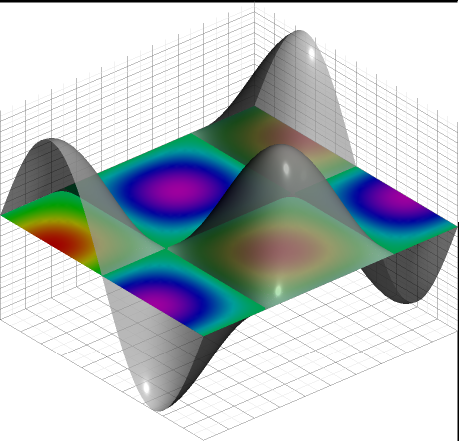
\includegraphics[width=1\linewidth,height=1\textheight,keepaspectratio]{rmarkdown-cookbook_files/figure-latex/elevation-1} 

}

\caption{Asymptote で作成した3Dグラフィック}\label{fig:elevation}
\end{figure}

PDF 出力に対しては追加の LaTeX パッケージが必要であることに注意してください. そうでないとこのようなエラーが出ることでしょう.

\begin{verbatim}
! LaTeX Error: File `ocgbase.sty' not found.
\end{verbatim}

このようなエラーが発生したなら, 欠けている LaTeX パッケージのインストール方法を\ref{install-latex-pkgs}節で確認してください.

上記の \texttt{asy} チャンクでは, \texttt{settings.prc = false} という設定を使いました. この設定がないと Asymptote は PDF 出力時にインタラクティブな 3D グラフィックを表示してしまいます. しかしインタラクティブなグラフィックは Acrobat Reader でのみ見ることができます. Acrobat Reader を使用しているなら, グラフを操作できます. 例えば図\ref{fig:elevation}ではマウス操作で3D平面を回転できます.

\hypertarget{r-ux3067ux30c7ux30fcux30bfux3092ux751fux6210ux3057-asymptote-ux306bux8aadux307fux8fbcux307eux305bux308b}{%
\subsection{R でデータを生成し Asymptote に読み込ませる}\label{r-ux3067ux30c7ux30fcux30bfux3092ux751fux6210ux3057-asymptote-ux306bux8aadux307fux8fbcux307eux305bux308b}}

ここでは, 最初に以下の R コードチャンクのように, R で生成したデータを CSV ファイルに保存します.

\begin{Shaded}
\begin{Highlighting}[numbers=left,,]
\NormalTok{x }\OtherTok{\textless{}{-}} \FunctionTok{seq}\NormalTok{(}\DecValTok{0}\NormalTok{, }\DecValTok{5}\NormalTok{, }\AttributeTok{l =} \DecValTok{100}\NormalTok{)}
\NormalTok{y }\OtherTok{\textless{}{-}} \FunctionTok{sin}\NormalTok{(x)}
\FunctionTok{writeLines}\NormalTok{(}\FunctionTok{paste}\NormalTok{(x, y, }\AttributeTok{sep =} \StringTok{","}\NormalTok{), }\StringTok{"sine.csv"}\NormalTok{)}
\end{Highlighting}
\end{Shaded}

それから Asymptote でこれを読み込み, データに基づいたグラフを描画し図\ref{fig:sine-curve} に示します. 以下が \texttt{asy} コードチャンクです.

\begin{Shaded}
\begin{Highlighting}[numbers=left,,]
\KeywordTok{import}\NormalTok{ graph;}
\NormalTok{size(}\DecValTok{400}\NormalTok{,}\DecValTok{300}\NormalTok{,IgnoreAspect);}
\NormalTok{settings.prc = }\KeywordTok{false}\NormalTok{;}

\CommentTok{// import data from csv file}
\NormalTok{file in=input(}\StringTok{"sine.csv"}\NormalTok{).line().csv();}
\NormalTok{real[][] a=in.dimension(}\DecValTok{0}\NormalTok{,}\DecValTok{0}\NormalTok{);}
\NormalTok{a=transpose(a);}

\CommentTok{// generate a path}
\NormalTok{path rpath = graph(a[}\DecValTok{0}\NormalTok{],a[}\DecValTok{1}\NormalTok{]);}
\NormalTok{path lpath = (}\DecValTok{1}\NormalTok{,}\DecValTok{0}\NormalTok{){-}{-}(}\DecValTok{5}\NormalTok{,}\DecValTok{1}\NormalTok{);}

\CommentTok{// find intersection}
\NormalTok{pair pA=intersectionpoint(rpath,lpath);}

\CommentTok{// draw all}
\NormalTok{draw(rpath,red);}
\NormalTok{draw(lpath,dashed + blue);}
\NormalTok{dot(}\StringTok{"$}\ErrorTok{\textbackslash{}d}\StringTok{elta$"}\NormalTok{,pA,NE);}
\NormalTok{xaxis(}\StringTok{"$x$"}\NormalTok{,BottomTop,LeftTicks);}
\NormalTok{yaxis(}\StringTok{"$y$"}\NormalTok{,LeftRight,RightTicks);}
\end{Highlighting}
\end{Shaded}

\begin{figure}

{\centering 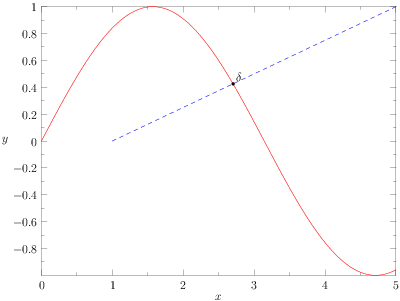
\includegraphics[width=1\linewidth,height=1\textheight,keepaspectratio]{rmarkdown-cookbook_files/figure-latex/sine-curve-1} 

}

\caption{R からデータを渡し Asymptote でグラフを描く}\label{fig:sine-curve}
\end{figure}

\hypertarget{eng-sass}{%
\section{Sass/SCSS で HTML ページをスタイリングする}\label{eng-sass}}

Sass (\url{https://sass-lang.com}) は CSS を拡張した言語\index{CSS!Sass}\index{Sass}で, 基本的な CSS で行っていた のよりはるかに柔軟な方法でルールを作成できます. これを学ぶことに関心があるなら, 公式ドキュメントを見てください.

R パッケージの \textbf{sass} \autocite{R-sass} \index{R パッケージ!sass} は SaSS を CSS にコンパイルするのに使用できます. \textbf{sass} パッケージに基づいて, \textbf{knitr} はコードチャンクを CSS にコンパイルするため2つの言語エンジン, \texttt{sass}\index{言語エンジン!sass} and \texttt{scss}\index{言語エンジン!scss} を読み込みます. Sass と SCSS の構文は互いに対応しているためです. 以下はチャンクヘッダが \texttt{\textasciigrave{}\textasciigrave{}\textasciigrave{}\{scss\}} である \texttt{scss} コードチャンクです.

\begin{Shaded}
\begin{Highlighting}[numbers=left,,]
\NormalTok{$font{-}stack: "HGS創英角ポップ体", "Comic Sans MS", cursive, sans{-}serif;}
\NormalTok{$primary{-}color: \#00FF00;}

\NormalTok{.book.font{-}family{-}1 \{}
\NormalTok{  font: 100\% $font{-}stack;}
\NormalTok{  color: $primary{-}color;}
\NormalTok{\}}
\end{Highlighting}
\end{Shaded}

\texttt{sass} エンジンも使うことができます. Sass 構文は SCSS 構文とわずかに異なります. 例えばこのように.

\begin{Shaded}
\begin{Highlighting}[]
\InformationTok{\textasciigrave{}\textasciigrave{}\textasciigrave{}\{sass\}}
\InformationTok{$font{-}stack: "HGS創英角ポップ体", "Comic Sans MS", cursive, sans{-}serif}
\InformationTok{$primary{-}color: \#00FF00}

\InformationTok{.book.font{-}family{-}1}
\InformationTok{  font: 100\% $font{-}stack}
\InformationTok{  color: $primary{-}color}
\InformationTok{\textasciigrave{}\textasciigrave{}\textasciigrave{}}
\end{Highlighting}
\end{Shaded}

あなたが\href{https://bookdown.org/yihui/rmarkdown-cookbook/eng-sass.html}{このセクションの HTML 版}を読んでいるなら, このページのフォントが Comic Sans に変化したことに気付くでしょう. これには驚いたかもしれませんが, パニックにならないでください, \href{https://twitter.com/andrewheiss/status/1250438044542361600}{あなたは脳卒中になどなっていません}.

\texttt{sass}/\texttt{scss} コードチャンクは \texttt{sass::sass()} 関数によってコンパイルされます. 現在はチャンクオプション \texttt{engine.opts} で CSS コードの出力スタイルをカスタマイズできます. 例えば \texttt{engine.opts = list(style = "expanded")} のように. デフォルトのスタイルは ``compressed'' です. これが何を意味するのか自信がないなら, \texttt{?sass::sass\_options} のヘルプを参照し, \texttt{output\_style} 引数の項目を探してください.

\hypertarget{managing-projects}{%
\chapter{プロジェクトを管理する}\label{managing-projects}}

大きなプロジェクトやレポートの作業をしている時, 全てのテキストとコードを1つの R Markdown 文書に置かずに, 代わりに小さな単位に分けたものをまとめたいかもしれません. この章では, R Markdown と関係する複数のファイルをまとめる方法を紹介します.

\hypertarget{source-script}{%
\section{外部の R スクリプトを実行する}\label{source-script}}

あなたの R Markdown 文書に大量のコードがあるなら, コードをいくらか外部 R スクリプトに配置し, \texttt{source()}\index{source()} か \texttt{sys.source()}\index{sys.source()} 経由で実行することを検討するとよいかもしれません. 例えばこのように.

\begin{Shaded}
\begin{Highlighting}[]
\InformationTok{\textasciigrave{}\textasciigrave{}\textasciigrave{}\{r, include=FALSE\}}
\InformationTok{source("your{-}script.R", local = knitr::knit\_global())}
\InformationTok{\# または sys.source("your{-}script.R", envir = knitr::knit\_global())}
\InformationTok{\textasciigrave{}\textasciigrave{}\textasciigrave{}}
\end{Highlighting}
\end{Shaded}

コードが適正な環境, つまり \texttt{knitr::knit\_global()}\index{knitr!knit\_global()} で評価されることを確実にするため, \texttt{sys.source()} の \texttt{envir} 引数または \texttt{source()} の \texttt{local} 引数を明示的に使うことをお薦めします. これらのデフォルトの値は適切な環境名でないことがあるかもしれません. あなたは間違った環境で変数を作成し, その後のチャンクでオブジェクトが見つからないことに驚くということになるかもしれないのです.

次に, R Markdown 文書では, これらのスクリプトで作成された, データや関数といったオブジェクトを使うことができます. これは R Markdown 文書を簡潔にするだけでなく, R コードの開発をより便利にする効果もあります. 例えば R コードのデバッグはしばしば, R Markdown よりピュアな R スクリプトでやるほうが簡単です.

出力を一切表示させずにスクリプトの実行のみをしたいので, 上記の例では \texttt{include = FALSE}\index{チャンクオプション!include} を使っていることに注意してください. 出力が欲しいのであればこのチャンクオプションを削除するか, \ref{hide-one}節で紹介した, 異なる種類の出力を選択的に隠したり表示したりするオプションを使用することもできます.

\hypertarget{option-code}{%
\section{外部スクリプトをチャンク内で読み込む}\label{option-code}}

\ref{source-script}節で紹介した \texttt{source()} の方法には欠点があります. それはデフォルトではソースコードを見ることができないという点です. \texttt{source(..., echo = TRUE)} を使うことはできますが, ソースコードに適切なシンタックスハイライトがなされません. 加えて\ref{source-script}節で言及したように, \texttt{source()} の \texttt{local} 引数について注意深くなる必要があります. この節ではこれらの問題とは関係ない代わりの方法を紹介します.

1つ以上の外部スクリプトがあるときは, 基本的にそれらを読み込みチャンクの \texttt{code} オプション\index{チャンクオプション!code}に中身を渡すこともできます. \texttt{code} オプションは文字列ベクトルをとり, そしてそれをコードチャンクの本文として扱うことができます. 以下に少しだけ例をお見せします.

\begin{itemize}
\item
  \texttt{code} オプションはソースコードの文字列ベクトルを取ることができます. これが例です.

\begin{Shaded}
\begin{Highlighting}[]
\InformationTok{\textasciigrave{}\textasciigrave{}\textasciigrave{}\{r, code=c(\textquotesingle{}1 + 1\textquotesingle{}, \textquotesingle{}if (TRUE) plot(cars)\textquotesingle{})\}}
\InformationTok{\textasciigrave{}\textasciigrave{}\textasciigrave{}}
\end{Highlighting}
\end{Shaded}
\item
  外部ファイルを読み込むこともできます.

\begin{Shaded}
\begin{Highlighting}[]
\InformationTok{\textasciigrave{}\textasciigrave{}\textasciigrave{}\{r, code=xfun::read\_utf8(\textquotesingle{}your{-}script.R\textquotesingle{})\}}
\InformationTok{\textasciigrave{}\textasciigrave{}\textasciigrave{}}
\end{Highlighting}
\end{Shaded}
\item
  大量のファイルを好きなだけ読み込むこともできます.

\begin{Shaded}
\begin{Highlighting}[]
\InformationTok{\textasciigrave{}\textasciigrave{}\textasciigrave{}\{r, include=FALSE\}}
\InformationTok{read\_files \textless{}{-} function(files) \{}
\InformationTok{  unlist(lapply(files, xfun::read\_utf8))}
\InformationTok{\}}
\InformationTok{\textasciigrave{}\textasciigrave{}\textasciigrave{}}

\InformationTok{\textasciigrave{}\textasciigrave{}\textasciigrave{}\{r, code=read\_files(c(\textquotesingle{}one.R\textquotesingle{}, \textquotesingle{}two.R\textquotesingle{}))\}}
\InformationTok{\textasciigrave{}\textasciigrave{}\textasciigrave{}}
\end{Highlighting}
\end{Shaded}
\end{itemize}

他の言語のスクリプトを読み込むこともできます. R Markdown で他の言語を使う方法は\ref{other-languages}章を確認してください. 以下に, さらに少しだけ R でないコードの例をお見せします.

\begin{itemize}
\item
  Python スクリプトを読み込む.

\begin{Shaded}
\begin{Highlighting}[]
\InformationTok{\textasciigrave{}\textasciigrave{}\textasciigrave{}\{python, code=xfun::read\_utf8(\textquotesingle{}script.py\textquotesingle{})\}}
\InformationTok{\textasciigrave{}\textasciigrave{}\textasciigrave{}}
\end{Highlighting}
\end{Shaded}
\item
  C++ ファイルを読み込む:

\begin{Shaded}
\begin{Highlighting}[]
\InformationTok{\textasciigrave{}\textasciigrave{}\textasciigrave{}\{Rcpp, code=xfun::read\_utf8(\textquotesingle{}file.cpp\textquotesingle{})\}}
\InformationTok{\textasciigrave{}\textasciigrave{}\textasciigrave{}}
\end{Highlighting}
\end{Shaded}
\end{itemize}

\texttt{code} オプションがあれば, 好きなエディタで複雑なコードの開発を行い, そして R Markdown 文書のコードチャンクに読み込むことができます.

\hypertarget{read-chunk}{%
\section{外部スクリプトから複数のコードチャンクを読み込む (*)}\label{read-chunk}}

\ref{option-code}節ではコードを単一のチャンクに読み込む方法を紹介しました. この節では外部スクリプトから複数のチャンクを読み取る方法の1つを紹介します. ポイントはスクリプト内のコードにラベルを付ける必要があるということ, そして R Markdown 文書のコードチャンクにも同じラベルを使用できるという点です. つまり外部スクリプトのコードを \texttt{knitr::read\_chunk()}\index{knitr!read\_chunk()} 関数を介して各コードチャンクに展開できるということです. スクリプトのブロックにラベルを付けるには, ラベルの後に \texttt{\#\# -\/-\/-\/-} と書きます (行の終わりにも好きな数のダッシュ記号を続けることができます). 例えばこのように, 1つのスクリプトには複数のラベル付けされたブロックを含めることができます.

\begin{Shaded}
\begin{Highlighting}[]
\DocumentationTok{\#\# {-}{-}{-}{-} test{-}a {-}{-}{-}{-}{-}{-}{-}{-}}
\DecValTok{1} \SpecialCharTok{+} \DecValTok{1}

\DocumentationTok{\#\# {-}{-}{-}{-} test{-}b {-}{-}{-}{-}{-}{-}{-}{-}}
\ControlFlowTok{if}\NormalTok{ (}\ConstantTok{TRUE}\NormalTok{) \{}
  \FunctionTok{plot}\NormalTok{(cars)}
\NormalTok{\}}
\end{Highlighting}
\end{Shaded}

上記のスクリプトのファイル名が \texttt{test.R} であるとします. R Markdown 文書ではこれを \texttt{knitr::read\_chunk()} 関数で読み込み, ラベルの付いたコードチャンク内で使うことができます. これが例です.

\begin{Shaded}
\begin{Highlighting}[]
\NormalTok{外部スクリプトを読み込む}

\InformationTok{\textasciigrave{}\textasciigrave{}\textasciigrave{}\{r, include=FALSE, cache=FALSE\}}
\InformationTok{knitr::read\_chunk(\textquotesingle{}test.R\textquotesingle{})}
\InformationTok{\textasciigrave{}\textasciigrave{}\textasciigrave{}}

\NormalTok{これで, 例えばこのようにコードを使用できる}

\InformationTok{\textasciigrave{}\textasciigrave{}\textasciigrave{}\{r, test{-}a, echo=FALSE\}}
\InformationTok{\textasciigrave{}\textasciigrave{}\textasciigrave{}}

\InformationTok{\textasciigrave{}\textasciigrave{}\textasciigrave{}\{r, test{-}b, fig.height=4\}}
\InformationTok{\textasciigrave{}\textasciigrave{}\textasciigrave{}}
\end{Highlighting}
\end{Shaded}

主に副作用のために \texttt{knitr::read\_chunk()} を使っていることに注意してください. つまりこの関数で読み込んだコードチャンクがキャッシュされていないことを確認してください (この説明は\ref{cache}節参照).

\ref{source-script}, \ref{option-code}節で紹介した方法のように, この方法は別の環境でコード開発できるという柔軟性をもたらしてくれます.

\hypertarget{child-document}{%
\section{子文書 (*)}\label{child-document}}

R Markdown 文書が長過ぎると思った時は, 短い文書\index{子文書}に分割して, チャンクオプション \texttt{child}\index{チャンクオプション!child} を使って子文書としてメインの文書に読み込ませることもできます. \texttt{child} オプションは子文書のファイルパスの文字列ベクトルを取ります. 例えばこのように.

\begin{Shaded}
\begin{Highlighting}[]
\InformationTok{\textasciigrave{}\textasciigrave{}\textasciigrave{}\{r, child=c(\textquotesingle{}one.Rmd\textquotesingle{}, \textquotesingle{}two.Rmd\textquotesingle{})\}}
\InformationTok{\textasciigrave{}\textasciigrave{}\textasciigrave{}}
\end{Highlighting}
\end{Shaded}

\textbf{knitr} のチャンクオプションは任意の R コードから値を取ることができるので, \texttt{child} オプションの応用の1つとしても文書の読み込みの条件付けがあります. 例えばあなたのレポートに, 上司が関心を持たなそうな技術的な詳細を含む補足文書があるなら, この付録をレポートに含むかどうかを制御する変数を使うこともできます.

\begin{Shaded}
\begin{Highlighting}[]
\NormalTok{あなたのボスにレポートを読ませるなら }\InformationTok{\textasciigrave{}BOSS\_MODE\textasciigrave{}}\NormalTok{ と }\InformationTok{\textasciigrave{}TRUE\textasciigrave{}}\NormalTok{ に変える}

\InformationTok{\textasciigrave{}\textasciigrave{}\textasciigrave{}\{r, include=FALSE\}}
\InformationTok{BOSS\_MODE \textless{}{-} FALSE}
\InformationTok{\textasciigrave{}\textasciigrave{}\textasciigrave{}}

\NormalTok{条件付きで補遺を読み込む}

\InformationTok{\textasciigrave{}\textasciigrave{}\textasciigrave{}\{r, child=if (!BOSS\_MODE) \textquotesingle{}appendix.Rmd\textquotesingle{}\}}
\InformationTok{\textasciigrave{}\textasciigrave{}\textasciigrave{}}
\end{Highlighting}
\end{Shaded}

あるいはまだ始まってないフットボールの試合の速報レポートを書いているなら, 試合結果に応じて異なる子文書を読み込むようにすることもできます. 例えば \texttt{child = if (winner == \textquotesingle{}ブラジル\textquotesingle{})\ \textquotesingle{}ブラジル.Rmd\textquotesingle{}\ else\ \textquotesingle{}ドイツ.Rmd\textquotesingle{}} のように. これで試合 (ここではドイツ対ブラジル) が終わり次第すぐに, レポートを提出できます.

子文書をコンパイルする別の方法として, \texttt{knitr::knit\_child()}\index{knitr!knit\_child()} 関数があります. この関数は R コードチャンクまたはインライン R コードの内部で呼び出すことができます. 例えばこのように.

\begin{Shaded}
\begin{Highlighting}[]
\InformationTok{\textasciigrave{}\textasciigrave{}\textasciigrave{}\{r, echo=FALSE, results=\textquotesingle{}asis\textquotesingle{}\}}
\InformationTok{res \textless{}{-} knitr::knit\_child(\textquotesingle{}child.Rmd\textquotesingle{}, quiet = TRUE)}
\InformationTok{cat(res, sep = \textquotesingle{}\textbackslash{}n\textquotesingle{})}
\InformationTok{\textasciigrave{}\textasciigrave{}\textasciigrave{}}
\end{Highlighting}
\end{Shaded}

\texttt{knit\_child()} 関数は knit された子文書の文字列ベクトルを返します. これは \texttt{cat()} とチャンクオプション \texttt{results = "asis"}\index{チャンクオプション!results} を使ってメインの文書に還元することができます.

テンプレートとして子文書を使うこともできますし, 毎回異なるパラメータを与えつつ \texttt{knit\_child()} 何度も呼び出すこともできます. 以下の例では \texttt{mpg} を従属変数として, そして \texttt{mtcars} データの残りの変数を説明変数として使って回帰分析を実行しています.

\begin{Shaded}
\begin{Highlighting}[]
\InformationTok{\textasciigrave{}\textasciigrave{}\textasciigrave{}\{r, echo=FALSE, results=\textquotesingle{}asis\textquotesingle{}\}}
\InformationTok{res \textless{}{-} lapply(setdiff(names(mtcars), \textquotesingle{}mpg\textquotesingle{}), function(x) \{}
\InformationTok{  knitr::knit\_child(text = c(}
\InformationTok{    \textquotesingle{}\#\# "\textasciigrave{}r x\textasciigrave{}" への回帰\textquotesingle{},}
\InformationTok{    \textquotesingle{}\textquotesingle{},}
\InformationTok{    \textquotesingle{}\textasciigrave{}\textasciigrave{}\textasciigrave{}\{r\}\textquotesingle{},}
\InformationTok{    \textquotesingle{}lm(mpg \textasciitilde{} ., data = mtcars[, c("mpg", x)])\textquotesingle{},}
\InformationTok{    \textquotesingle{}\textasciigrave{}\textasciigrave{}\textasciigrave{}\textquotesingle{},}
\InformationTok{    \textquotesingle{}\textquotesingle{}}
\InformationTok{  ), envir = environment(), quiet = TRUE)}
\InformationTok{\})}
\InformationTok{cat(unlist(res), sep = \textquotesingle{}\textbackslash{}n\textquotesingle{})}
\InformationTok{\textasciigrave{}\textasciigrave{}\textasciigrave{}}
\end{Highlighting}
\end{Shaded}

上記の例を自己完結的なものにするために, \texttt{knit\_child()} にファイルを入力するのではなく \texttt{text} 引数に R Markdown コンテンツを渡しました. もちろんファイルにコンテンツを書き出し, \texttt{knit\_child()} にファイルパスを渡すこともできます. 例えば以下の例では \texttt{template.Rmd} という名前のファイルに保存しています.

\begin{Shaded}
\begin{Highlighting}[]
\FunctionTok{\#\# "\textasciigrave{}r x\textasciigrave{}" への回帰}

\InformationTok{\textasciigrave{}\textasciigrave{}\textasciigrave{}\{r\}}
\InformationTok{lm(mpg \textasciitilde{} ., data = mtcars[, c("mpg", x)])}
\InformationTok{\textasciigrave{}\textasciigrave{}\textasciigrave{}}
\end{Highlighting}
\end{Shaded}

そして代わりにファイルを knit します.

\begin{Shaded}
\begin{Highlighting}[numbers=left,,]
\NormalTok{res }\OtherTok{\textless{}{-}} \FunctionTok{lapply}\NormalTok{(}\FunctionTok{setdiff}\NormalTok{(}\FunctionTok{names}\NormalTok{(mtcars), }\StringTok{\textquotesingle{}mpg\textquotesingle{}}\NormalTok{), }\ControlFlowTok{function}\NormalTok{(x) \{}
\NormalTok{  knitr}\SpecialCharTok{::}\FunctionTok{knit\_child}\NormalTok{(}
    \StringTok{\textquotesingle{}template.Rmd\textquotesingle{}}\NormalTok{, }\AttributeTok{envir =} \FunctionTok{environment}\NormalTok{(), }\AttributeTok{quiet =} \ConstantTok{TRUE}
\NormalTok{  )}
\NormalTok{\})}
\FunctionTok{cat}\NormalTok{(}\FunctionTok{unlist}\NormalTok{(res), }\AttributeTok{sep =} \StringTok{\textquotesingle{}}\SpecialCharTok{\textbackslash{}n}\StringTok{\textquotesingle{}}\NormalTok{)}
\end{Highlighting}
\end{Shaded}

\hypertarget{keep-files}{%
\section{グラフ画像ファイルを残す}\label{keep-files}}

ほとんどの R Markdown 出力フォーマットはデフォルトで \texttt{self\_contained = TRUE}\index{出力オプション!self\_contained} オプションを使用しています. これは R グラフを出力文書に埋め込ませるので, 出力文書を閲覧する時には中間ファイルは必要ありません. 結果としてグラフ画像のフォルダ (典型的には \texttt{\_files} という接尾語があります) は Rmd 文書がレンダリングされた後に削除されます\index{図!ファイルを残す}.

ときにはグラフ画像ファイルを残したいかもしれません. 例えば画像ファイルを別個に提出するよう著者に要求する学術誌があります. R Markdown ではこれらのファイルの自動削除を回避する3通りの方法があります.

\begin{enumerate}
\def\labelenumi{\arabic{enumi}.}
\item
  出力フォーマットがサポートしているなら, \texttt{self\_contained = FALSE} オプションを使う. 例えばこのように.

\begin{Shaded}
\begin{Highlighting}[]
\FunctionTok{output}\KeywordTok{:}
\AttributeTok{  }\FunctionTok{html\_document}\KeywordTok{:}
\AttributeTok{    }\FunctionTok{self\_contained}\KeywordTok{:}\AttributeTok{ }\CharTok{false}
\end{Highlighting}
\end{Shaded}

  しかし, これはグラフ画像ファイルが出力文書に埋め込まれません. それがあなたにとって望ましくないなら, 次の2つの方法を検討することもできます.
\item
  最低いずれか1つのコードチャンクでキャッシュ (\ref{cache}節参照) を有効にする. キャッシュが有効な時は R Markdown は画像フォルダを削除しません.
\item
  出力フォーマットがサポートしているなら, \texttt{keep\_md = TRUE}\index{出力オプション!keep\_md} オプションを使用する. 例えばこのように.

\begin{Shaded}
\begin{Highlighting}[]
\FunctionTok{output}\KeywordTok{:}
\AttributeTok{  }\FunctionTok{word\_document}\KeywordTok{:}
\AttributeTok{    }\FunctionTok{keep\_md}\KeywordTok{:}\AttributeTok{ }\CharTok{true}
\end{Highlighting}
\end{Shaded}

  R Markdown が Markdown 中間出力ファイルを保存するよう指示した時, 同時に画像フォルダも保存されます.
\end{enumerate}

\hypertarget{working-directory}{%
\section{R コードチャンク用の作業ディレクトリ}\label{working-directory}}

デフォルトでは R コードチャンクの作業ディレクトリ\index{作業ディレクトリ}は Rmd 文書のあるディレクトリです. 例えば Rmd ファイルのパスが \texttt{\textasciitilde{}/Downloads/foo.Rmd} であるなら, R コードチャンクが評価される作業ディレクトリは \texttt{\textasciitilde{}/Downloads/} になります. これはチャンク内で外部ファイルを相対パスで参照するとき, そのパスは Rmd ファイルのあるディレクトリからの相対パスであることを知る必要があることを意味します. 前述の例の Rmd ファイルでは, コードチャンク内での \texttt{read.csv("data/iris.csv")} は \texttt{\textasciitilde{}/Downloads/data/iris.csv} から CSV ファイルを読み込むことを意味しています.

よく分からない時は, \texttt{getwd()} をコードチャンクに追加して文書をコンパイルし, \texttt{getwd()} の出力を確認することができます.

時には他のディレクトリを作業ディレクトリとして使いたいかもしれません. たいていの場合は作業ディレクトリの変更方法は \texttt{setwd()} ですが, \texttt{setwd()} は R Markdown あるいは他の \textbf{knitr} ソース文書では一貫性がないことに注意してください. これは \texttt{setwd()} が現在のコードチャンクに対して動作し, 作業ディレクトリはこのコードチャンクが評価された後に元に戻ることを意味します.

全てのコードチャンクに対して作業ディレクトリを変更したい場合, 文書の冒頭の \texttt{setup} コードチャンクでこのように設定することもできます\index{knitr!root.dir}\index{knitr!opts\_knit}.

\begin{Shaded}
\begin{Highlighting}[]
\InformationTok{\textasciigrave{}\textasciigrave{}\textasciigrave{}\{r, setup, include=FALSE\}}
\InformationTok{knitr::opts\_knit$set(root.dir = \textquotesingle{}/tmp\textquotesingle{})}
\InformationTok{\textasciigrave{}\textasciigrave{}\textasciigrave{}}
\end{Highlighting}
\end{Shaded}

これは以降の全てのコードチャンクの作業ディレクトリを変更します.

RStudio を使用しているなら, 作業ディレクトリをメニュの \texttt{Tools -\textgreater{}\ Global\ Options\ -\textgreater{}\ R\ Markdown} からも選択できます\index{RStudio!作業ディレクトリ} (図\ref{fig:rmd-wd}参照). デフォルトの作業ディレクトリは Rmd ファイルのディレクトリで, 他に2つの選択肢があります. ``Current'' オプションで R コンソールの現在の作業ディレクトリを使うか, ``Project'' オプションで Rmd ファイルの含まれているプロジェクトのルートディレクトリを作業ディレクトリとして使うこともできます.

\begin{figure}

{\centering 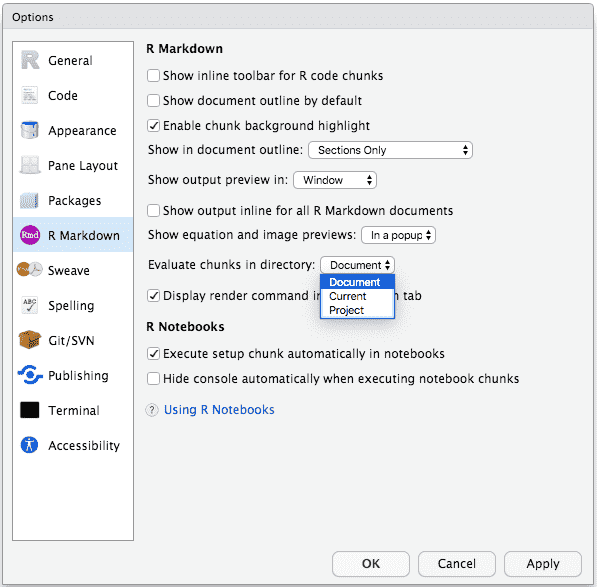
\includegraphics[width=1\linewidth,height=1\textheight,keepaspectratio]{JP/images/rmd-wd} 

}

\caption{R Studio で R Markdown 文書用のデフォルトの作業ディレクトリを変更する}\label{fig:rmd-wd}
\end{figure}

RStudio では, 図\ref{fig:knit-wd}で見せるように, 個別の Rmd 文書をそれぞれ固有の作業ディレクトリで knit することもできます. ``Knit Directory'' を変更し ``Knit'' ボタンをクリックした後で, \textbf{knitr} はコードチャンクの評価に新しい作業ディレクトリを使用します. これらの全ての設定は既に言及した \texttt{knitr::opts\_knit\$set(root.dir = ...)} に集約されています. よってあなたがこれらの選択のいずれにも満足しないのなら, \texttt{knitr::opts\_knit\$set()} を使いご自分でディレクトリを指定できます.

\begin{figure}

{\centering 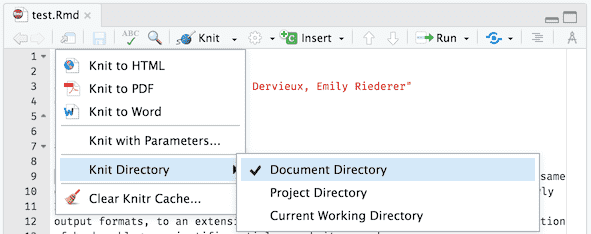
\includegraphics[width=1\linewidth,height=1\textheight,keepaspectratio]{JP/images/knit-wd} 

}

\caption{RStudio の他の使用可能な作業ディレクトリで Rmd 文書を knit する}\label{fig:knit-wd}
\end{figure}

作業ディレクトリに関して完全に正しい選択というものはありません. それぞれに長所と短所があります.

(\textbf{knitr} のデフォルト) Rmd 文書のディレクトリをコードチャンクの作業ディレクトリとして使うなら, ファイルパスは Rmd 文書からの相対パスだと想定します. これは ウェブブラウザで相対パスを扱うのと似ています. 例えば 例えば \texttt{https://www.example.org/path/to/page.html} という HTML ページでの画像 \texttt{\textless{}img\ src="foo/bar.png"\ /\textgreater{}} に対して, ウェブブラウザが \texttt{https://www.example.org/path/to/foo/bar.png} から画像を取得しようとするのと似ています. 言い換えるなら, 相対パス \texttt{foo/bar.png} は HTML ファイルのディレクトリ \texttt{https://www.example.org/path/to/} からの相対位置です.

\begin{verbatim}
このアプローチの利点は Rmd ファイルを参照するファイルと**一緒に**, 相対的な位置関係を保っている限りどこへでも自由に移動できることです. 上記の HTML ページと画像の例では, `page.html` と `foo/bar.png` を `https://www.example.org/another/path/` へ一緒に移動させることができます. そしてあなたは `<img />` の `src` 属性の相対パスを更新する必要はありません.

Rmd 文書の相対パスを「Rmd ファイルからの相対位置」とは対照的に「Rコンソールの作業ディレクトリからの相対位置」と考えるのを好むユーザもいます. よって **knitr** のデフォルトディレクトリは混乱を招きます. 私が **knitr** を設計する際に R コンソールの作業ディレクトリをデフォルトで使わないようにした理由は, ユーザがいつでも `setwd()` で作業ディレクトリを変更できるようにするためでした. この作業ディレクトリが安定している保証はありません.  毎度のようにユーザが `setwd()` をコンソールで呼び出すと, Rmd 文書内のファイルパスが無効になるリスクがあります. ファイルパスが `setwd()` という外部要因に依存していて, それが Rmd ファイルの制御の手から離れているというのは恐ろしいことでしょう. 相対パスを考慮して, Rmd ファイルを「宇宙の中心」として扱うのなら, Rmd ファイル内のパスは安定するでしょう.

その上, あなたが相対パスを考慮するのが難しすぎるのでやりたくないのなら, 図\\ref{fig:rmd-relative}のように RStudio 上で自動補完機能を使ってファイルパスを入力することもできます. RStudio は Rmd ファイルからの相対パスを補完しようと試みます.
\end{verbatim}

\begin{itemize}
\item
  R コンソールの作業ディレクトリはプログラミング的あるいは対話的に文書を knit するのに良い選択になりうるでしょう. 例えばループ中に文書を複数回 knit し, その毎回で異なる作業ディレクトリを使い, ディレクトリ内の異なるデータファイルを読み込む (ファイル名は同じとします) こともできます. この種の作業ディレクトリは \textbf{ezknitr} パッケージ\index{R パッケージ!ezknitr} \autocite{R-ezknitr} で支持されており, 実質的に \textbf{knitr} のコードチャンクのために作業ディレクトリを変更するために \texttt{knitr::opts\_knit\$set(root.dir)} を使用しています.
\item
  プロジェクトディレクトリを作業ディレクトリとして使うことには明確な前提が要求されます. そもそもプロジェクト (例えば RStudio のプロジェクトか, バージョン管理プロジェクト) を使わなければならないということです. これはこのアプローチの欠点となりえます. この種の作業ディレクトリの利点はあらゆる Rmd 文書内の全ての相対パスがプロジェクトのルートディレクトリからの相対パスになることです. よってプロジェクト内で Rmd ファイルがどこにあるかを考えたり, 対応する他のファイルの場所を調整したりする必要はありません. この種の作業ディレクトリは \textbf{here} パッケージ\index{R パッケージ!here} \autocite{R-here} で支持されており, このパッケージは渡された相対パスを解決し絶対パスを返す \texttt{here::here()} 関数を提供しています (相対パスはプロジェクトのルートからの相対であることを忘れないでください). 欠点は参照されているファイルを Rmd ファイルとともにプロジェクト内の他の場所に移動させた時に, Rmd 文書内の参照パスを更新する必要があることです. Rmd ファイルを他の人と共有する時は, プロジェクト全体も共有しなければなりません.

  これらの種類のパスは HTML でのプロトコルやドメインのない絶対パスと似ています. 例えば \texttt{https://www.example.org/path/to/page.html} というページの画像 \texttt{\textless{}img\ src="/foo/bar.png"\ /\textgreater{}} はウェブサイトのルートディレクトリ以下の画像を参照しています. つまり \texttt{https://www.example.org/foo/bar.png} です. 画像の \texttt{src} 属性の先頭の \texttt{/} はウェブサイトのルートディレクトリを表しています. 絶対パスと相対パスについてもっと学びたい (あるいはもっと混乱したい) なら, \href{https://bookdown.org/yihui/blogdown/html.html}{\textbf{blogdown} 本の Appendix B.1} \autocite{blogdown2017} を見てください.
\end{itemize}

うんざりさせられる作業ディレクトリ問題は相対パスに対処している時に発生した次のような疑問に端を発します. 「\textbf{何に対して相対的なの?}」と. 既に言及したように, いろいろな人がいろいろな好みを持っており, 完全に正しい回答はありません.

\begin{figure}

{\centering 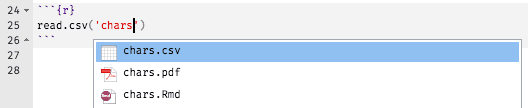
\includegraphics[width=1\linewidth,height=1\textheight,keepaspectratio]{JP/images/rmd-relative} 

}

\caption{RStudio 上で Rmd 文書のファイルパスを自動補完する}\label{fig:rmd-relative}
\end{figure}

\hypertarget{package-vignette}{%
\section{R パッケージのビネット}\label{package-vignette}}

R パッケージの開発を経験したか, プロジェクトで自作関数の明瞭なドキュメントや厳格なテストが要求されたなら, あなたはプロジェクトを R パッケージと結びつけることを検討するかもしれません. R パッケージの作り方が分からないなら, RStudio IDE でメニューバーの \texttt{File -\textgreater{}\ New\ Project} をクリックし, プロジェクトの種類に R パッケージを選ぶことで簡単に始めることができます\index{R パッケージ!ビネット}\index{ビネット}\index{vignette|see{ビネット}}.

プロジェクトの管理に R パッケージを使うことには多くの利益があります. 例えば \texttt{data/} フォルダにデータを置き, \texttt{R/} に R コードを書き, 例えば \textbf{roxygen2} パッケージ \autocite{R-roxygen2}\index{R パッケージ!roxygen2} を使用して, ドキュメントを \texttt{man/} に生成し, \texttt{test/} には単体テストを追加できます. R Markdown のレポートなら \texttt{vignette/} にパッケージのビネットとして書くことができます. ビネット内ではデータセットを読み込みパッケージ内の関数を呼び出せます. (\texttt{R CMD build} コマンドか RStudio で) パッケージをビルドする時に, ビネットは自動でコンパイルされます.

R Markdown でパッケージのビネットを作成するには, 最も簡単な方法は RStudio のメニュー \texttt{File -\textgreater{}\ New\ File\ -\textgreater{}\ R\ Markdown\ -\textgreater{}\ From\ Template}\index{RStudio!ビネットのテンプレート}を経由するものです (図\ref{fig:package-vignette}参照). それから \textbf{rmarkdown} パッケージから ``Package Vignette'' を選択し, ビネットのテンプレートを得ます. テンプレートの, タイトル・著者・その他のメタデータを変更したら, レポートの本文を書き始めることができます.

\begin{figure}

{\centering 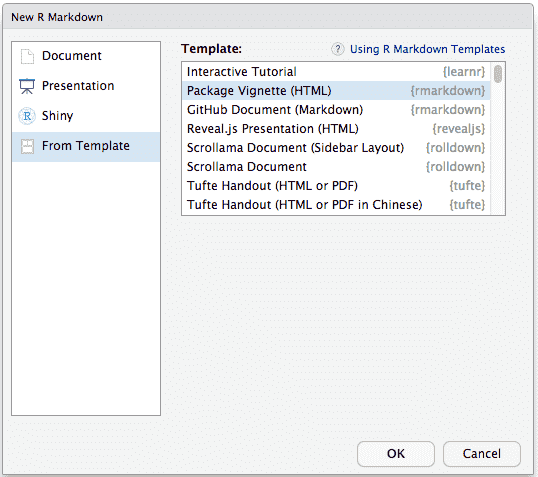
\includegraphics[width=1\linewidth,height=1\textheight,keepaspectratio]{JP/images/package-vignette} 

}

\caption{RStudio でパッケージのビネットを作成する}\label{fig:package-vignette}
\end{figure}

代わりに, \textbf{usethis}\index{R パッケージ!usethis} \autocite{R-usethis} をインストールしビネットのスケルトンを作成するのに \texttt{usethis::use\_vignette()}\index{usethis!use\_vignette()} 関数を使うこともできます. 以下はパッケージのビネットの YAML フロントマターの典型的な姿です\index{YAML!ビネットのフロントマター}.

\begin{Shaded}
\begin{Highlighting}[]
\PreprocessorTok{{-}{-}{-}}
\FunctionTok{title}\KeywordTok{:}\AttributeTok{ }\StringTok{"ビネットのタイトル"}
\FunctionTok{author}\KeywordTok{:}\AttributeTok{ }\StringTok{"ビネットの著者"}
\FunctionTok{output}\KeywordTok{:}\AttributeTok{ rmarkdown::html\_vignette}
\FunctionTok{vignette}\KeywordTok{: }\CharTok{\textgreater{}}
\NormalTok{  \%\textbackslash{}VignetteIndexEntry\{ビネットのタイトル\}}
\NormalTok{  \%\textbackslash{}VignetteEngine\{knitr::rmarkdown\}}
\NormalTok{  \%\textbackslash{}VignetteEncoding\{UTF{-}8\}}
\PreprocessorTok{{-}{-}{-}}
\end{Highlighting}
\end{Shaded}

\texttt{title} フィールドと \texttt{\textbackslash{}VignetteIndexEntry\{\}} コマンドの両方で, ビネットのタイトルを変更する必要があることに注意してください. 上記のビネット情報の他にも, パッケージの \texttt{DESCRIPTION} ファイルにさらに2つ必要なことがあります.

\begin{enumerate}
\def\labelenumi{\arabic{enumi}.}
\item
  \texttt{DESCRIPTION} ファイルに \texttt{VignetteBuilder: knitr} を指定する.
\item
  \texttt{DESCRIPTION} ファイルに \texttt{Suggests: knitr, rmarkdown} を指定する.
\end{enumerate}

ビネット出力フォーマットは HTML でなくてもよいです. PDF でも可能なので, \texttt{output: pdf\_document} を使うこともできます. \texttt{beamer\_presentation} や \texttt{tufte::tufte\_html} のような, HTML か PDF を作成する他の出力フォーマットでも大丈夫です. しかし, 現時点では R は HTML と PDF のビネットのみを認識します.

\hypertarget{package-template}{%
\section{R パッケージの R Markdown テンプレート}\label{package-template}}

\ref{package-vignette}節の図\ref{fig:package-vignette}は編集可能なパッケージビネットのテンプレートを \textbf{rmarkdown} パッケージから取得する工程を表しています. この R Markdown ファイルは R パッケージのビネットに対して適切なメタデータが入力済みです\index{R パッケージ!R Markdown テンプレート}\index{テンプレート!R Markdown}.

同様に, R パッケージに, (この図で示しているように) ユーザが RStudio IDE を通してアクセスできるか, あるいはどのプラットフォーム上でも \texttt{rmarkdown::draft()}\index{rmarkdown!draft} 関数でアクセスできる Markdown テンプレートを同梱してもよいです.

\hypertarget{ux30c6ux30f3ux30d7ux30ecux30fcux30c8ux306eux30e6ux30fcux30b9ux30b1ux30fcux30b9template-use-cases}{%
\subsection{テンプレートのユースケースTemplate use-cases}\label{ux30c6ux30f3ux30d7ux30ecux30fcux30c8ux306eux30e6ux30fcux30b9ux30b1ux30fcux30b9template-use-cases}}

テンプレートはカスタマイズされた文書構造・スタイル・コンテンツを共有するのに便利な方法です. 多くのすばらしい例が世に出回っています\index{R パッケージ!R Markdown テンプレート}.

多くのテンプレートは入力済みのメタデータによって文書構造とスタイルを追加しています. すでに \textbf{rmarkdown} パッケージの (HTML の) ビネットテンプレートを例としてお見せしました. 同様に, \textbf{rmdformats} パッケージ \autocite{R-rmdformats} は様々なカスタムスタイル関数を \texttt{output} オプションに渡すテンプレートがいくつも提供されています.

その他のテンプレートはパッケージを要求する文書構造を実現しています. 例えば *pagedown\textbf{ パッケージ \autocite{R-pagedown} はポスター・履歴書・その他のページレイアウト用に無数のテンプレートを同梱しています. 同様に }xaringan** パッケージ \autocite{R-xaringan} の忍者風のプレゼンテーションテンプレートは様々なスライドフォーマットのオプションに対する構文を実現しています.

テンプレートはパッケージの機能と構文を実証していることもあります. 例えば \textbf{flexdashboard} パッケージ \autocite{R-flexdashboard} と \textbf{learnr} package \autocite{R-learnr} パッケージはサンプルのダッシュボートとチュートリアルをそれぞれ作成するためにパッケージから関数を呼び出すコードチャンクのあるテンプレートを同梱しています.

同様に, テンプレートは定型的なコンテンツ様式をも含んでいるかもしれません. 例えば \textbf{rticles} パッケージ \autocite{R-rticles} は R Markdown 出力を, 様々な学術誌で要求されるスタイルとガイドラインに沿って調整する, 多くのそのようなテンプレートを提供します. 様式に沿ったコンテンツは, 四半期レポートを作成するチームのような組織的な設定においても便利です.

\hypertarget{ux30c6ux30f3ux30d7ux30ecux30fcux30c8ux306eux6e96ux5099}{%
\subsection{テンプレートの準備}\label{ux30c6ux30f3ux30d7ux30ecux30fcux30c8ux306eux6e96ux5099}}

\textbf{usethis} パッケージ \autocite{R-usethis} にはテンプレートの作成に役に立つ関数があります. \texttt{usethis::use\_rmarkdown\_template("テンプレート名")}\index{usethis!use\_rmarkdown\_template()} を実行すると, 要求されたディレクトリ構造とファイルが自動で作成されます. そしてあなたは自分のテンプレート名を与えるべきです.

代わりに自分のテンプレートを手動で準備したいなら, \texttt{inst/rmarkdown/templates} のサブディレクトリに作成してください. このディレクトリ内に, 少なくとも2つのファイルを保存する必要があります.

\begin{enumerate}
\def\labelenumi{\arabic{enumi}.}
\item
  \texttt{template.yaml} という名前のファイル. これは RStudio IDE に, 人間が判読できるテンプレートの名称といった基本的なメタデータを与えます. 最低でも, このファイルは \texttt{name} と \texttt{description} フィールドを持っているべきです. 例えばこのように.

\begin{Shaded}
\begin{Highlighting}[]
\FunctionTok{name}\KeywordTok{:}\AttributeTok{ テンプレートの例}
\FunctionTok{description}\KeywordTok{:}\AttributeTok{ このテンプレートが何をするか}
\end{Highlighting}
\end{Shaded}

  テンプレートが選択された時に新しいディレクトリを作成してほしいなら, \texttt{create\_dir: true} を含めることもできます. 例えば \href{https://github.com/rstudio/learnr/blob/master/inst/rmarkdown/templates/tutorial/template.yaml}{\textbf{learnr} パッケージのテンプレート}は \texttt{create\_dir: true} を設定しており, 一方で \href{https://github.com/rstudio/flexdashboard/blob/master/inst/rmarkdown/templates/flex_dashboard/template.yaml}{\textbf{flexdashboard} パッケージのテンプレート} はデフォルトの \texttt{create\_dir: false} を使用しています. 様々なユーザの意図に気付くために, これらのテンプレートを RStudio で開いてみることもできます.
\item
  \texttt{skeleton/skeleton.Rmd} 内保存された R Markdown 文書ファイル. これは R Markdown 文書に挿入したいものを含めることができます.
\end{enumerate}

オプションとして, \texttt{skeleton} フォルダにはスタイルシートや画像といった, テンプレートで使われる追加のリソースを含めることができます. これらのファイルはテンプレートとともにユーザのコンピュータに読み込まれます.

R Markdown のカスタムテンプレートを作るためのさらに詳細な情報は, \href{https://rstudio.github.io/rstudio-extensions/rmarkdown_templates.html}{RStudio Extensions} と \emph{R Markdown Definitive Guide} \autocite{rmarkdown2018} の \href{https://bookdown.org/yihui/rmarkdown/document-templates.html}{Document Templates chapter} を参照してください.

\hypertarget{bookdown}{%
\section{\texorpdfstring{\textbf{bookdown} で本や長いレポートを書く}{bookdown で本や長いレポートを書く}}\label{bookdown}}

\textbf{bookdown} パッケージ \autocite{R-bookdown}\index{R パッケージ!bookdown} は複数の R Markdown 文書で構成される長い文書\index{本}を作成するように設計されています. 例えば本を執筆したいなら, 章ごとに別々の Rmd ファイルに書き, これらのファイルを本にコンパイルするのに \textbf{bookdown} を使うことが可能です.

RStudio ユーザーにとって最も簡単な始め方は, 図\ref{fig:bookdown-project}で見られるように IDE 上で \texttt{File -\textgreater{}\ New\ Project\ -\textgreater{}\ New\ Directory\ -\textgreater{}\ Book\ Project\ using\ bookdown} を選んで \textbf{bookdown} プロジェクト\index{RStudio!bookdown プロジェクト}を作成することです.

RStudio を使っていないか, コンソールから作業するのが好きなら, \texttt{bookdown:::bookdown\_skeleton(\textquotesingle{}本のディレクトリ\textquotesingle{})} 関数を呼ぶことで同じものを生み出せます.

\begin{figure}

{\centering 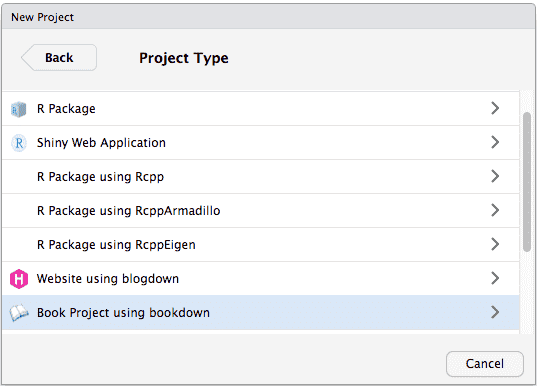
\includegraphics[width=1\linewidth,height=1\textheight,keepaspectratio]{JP/images/bookdown-project} 

}

\caption{RStudio で bookdown プロジェクトを作成する}\label{fig:bookdown-project}
\end{figure}

使用法を実演するために, 同じディレクトリに3つのファイルを含めた最低限の例を用意しました.

\begin{Shaded}
\begin{Highlighting}[]
\NormalTok{directory}
\NormalTok{  |{-} index.Rmd}
\NormalTok{  |{-} 01{-}導入.Rmd}
\NormalTok{  |{-} 02{-}分析.Rmd}
\end{Highlighting}
\end{Shaded}

以下に各ファイルの中身とそれぞれの役目を示します.

\begin{itemize}
\item
  \textbf{index.Rmd}:

\begin{Shaded}
\begin{Highlighting}[]
\CommentTok{{-}{-}{-}}
\AnnotationTok{title:}\CommentTok{ "最低限の bookdown プロジェクト"}
\AnnotationTok{site:}\CommentTok{ bookdown::bookdown\_site}
\AnnotationTok{output:}\CommentTok{ bookdown::gitbook}
\CommentTok{{-}{-}{-}}

\FunctionTok{\# はじめに \{{-}\}}

\NormalTok{なにか書く}
\end{Highlighting}
\end{Shaded}
\end{itemize}

最初のファイルは典型的には \texttt{index.Rmd} と呼ばれます. YAML フロントマターを与える唯一の Rmd ファイルとなるべきです. また, 単一の Rmd ファイルをレンダリングするのではなく, 全ての Rmd ファイルをビルドするために \textbf{bookdown} を使うことを \textbf{rmarkdown} に知らせるための特殊な YAML フィールド, \texttt{site: bookdown::bookdown\_site} を含むべきです. \texttt{bookdown::gitbook} ・ \texttt{bookdown::pdf\_book} ・ \texttt{bookdown::word\_document2} ・ \texttt{bookdown::epub\_book} といった \textbf{bookdown} 出力フォーマットをいずれも使うことができます.

次の2つの Rmd ファイルは2つの章になります.

\begin{itemize}
\item
  \textbf{01-導入.Rmd:}

\begin{Shaded}
\begin{Highlighting}[]
\FunctionTok{\# 第1章}

\NormalTok{これは第1章です.}
\end{Highlighting}
\end{Shaded}
\item
  \textbf{02-分析.Rmd}:

\begin{Shaded}
\begin{Highlighting}[]
\FunctionTok{\# 第2章}

\NormalTok{これは第2章です.}
\end{Highlighting}
\end{Shaded}
\end{itemize}

これらの Rmd ファイルをレンダリングするために, \texttt{rmarkdown::render()} の代わりに \texttt{bookdown::render\_book(\textquotesingle{}index.Rmd\textquotesingle{})} を呼ぶべきです. その内部では, デフォルトでは \textbf{bookdown} が全ての Rmd ファイルを1つの Rmd に結合し, コンパイルします. ファイルは名前順に結合されます. 上記の例でファイル名の頭に数字を付けたのはそれが理由です.

\textbf{bookdown} プロジェクトをカスタマイズすることができる設定は多くあります. \textbf{bookdown} のより包括的な概要として, \textbf{rmarkdown} 本 \autocite{rmarkdown2018} の Chapter 18 を読むこともできます. 完全なドキュメントは \textbf{bookdown} 本 \autocite{bookdown2016} になります.

\hypertarget{blogdown}{%
\section{\texorpdfstring{\textbf{blogdown} でウェブサイトを構築する}{blogdown でウェブサイトを構築する}}\label{blogdown}}

R Markdown に基づいたウェブサイトを構築したいなら, \textbf{blogdown} パッケージ\index{R パッケージ!blogdown} \autocite{R-blogdown} の使用を検討するとよいでしょう. 最も簡単な始め方は図\ref{fig:bookdown-project}で見られるように RStudio メニューから \texttt{File -\textgreater{}\ New\ Project\ -\textgreater{}\ New\ Directory\ -\textgreater{}\ Website\ using\ blogdown} を選ぶことです. これまで \textbf{blogdown} を使ったことがないのなら, ダイアログボックスのデフォルト設定をを使うこともできます. そうでないなら, ウェブサイトのテーマのようにカスタマイズできます. RStudio を使用していないのなら, 新しいウェブサイトを作る空のディレクトリで \texttt{blogdown::new\_site()} 関数を呼び出すことができます.

ウェブサイトのプロジェクトには Rmd 文書をいくつふくめてもよいです. これらは通常のページか, ブログの記事にできます. あなたのウェブサイトに表示されるものは自動的にかつ動的に生成されるので, R Markdown によってあなたは簡単に自分のウェブサイトを管理できるようになります.

ウェブサイトの管理の基本的なワークフローとこのパッケージの概要のために, \textbf{blogdown} 本 \autocite{blogdown2017} の \href{https://bookdown.org/yihui/blogdown/get-started.html}{Chapter 1} を読むことをお薦めします.

\hypertarget{workflow}{%
\chapter{ワークフロー}\label{workflow}}

この章では R Markdown プロジェクトの運用のみならず個別の R Markdown 文書で作業する際の豆知識を紹介します. \emph{R for Data Science}\footnote{邦題『Rで学ぶデータサイエンス』} \autocite{wickham2016} の \href{https://r4ds.had.co.nz/r-markdown-workflow.html}{Chapter 30} も確認するとよいでしょう. ここには (R Markdown 文書を含む) 分析ノートの使用に関する豆知識が簡単に紹介されています. Nicholas Tierney も \href{https://rmd4sci.njtierney.com/workflow.html}{\emph{R Markdown for Scientists}.} でワークフローについて議論しています.

\hypertarget{rstudio-shortcuts}{%
\section{RStudio のキーボード・ショートカットを使う}\label{rstudio-shortcuts}}

R・ \textbf{rmarkdown} パッケージ・Pandoc がインストールされているかぎり, R Markdown のフォーマットはあなたの選ぶどんなテキストエディタでも使用できます. しかし, RStudio\index{RStudio!キーボード・ショートカット}は R Markdownと深く統合されているので, 円滑に R Markdown と作業できます.

あらゆる IDE (統合開発環境) のように, RStudio にはキーボード・ショートカットがあります. 完全な一覧はメニューの \texttt{Tools -\textgreater{}\ Keyboard\ Shortcuts\ Help} で見られます. R Markdown に関連する最も便利なショートカットを表\ref{tab:shortcuts}にまとめました.

\begin{table}

\caption{\label{tab:shortcuts}R Markdown に関連する RStudio のキーボード・ショートカット}
\centering
\begin{tabular}[t]{lll}
\toprule
Task & Windows \& Linux & macOS\\
\midrule
Insert R chunk & Ctrl+Alt+I & Command+Option+I\\
Preview HTML & Ctrl+Shift+K & Command+Shift+K\\
Knitr document (knitr) & Ctrl+Shift+K & Command+Shift+K\\
Compile Notebook & Ctrl+Shift+K & Command+Shift+K\\
Compile PDF & Ctrl+Shift+K & Command+Shift+K\\
\addlinespace
Run all chunks above & Ctrl+Alt+P & Command+Option+P\\
Run current chunk & Ctrl+Alt+C & Command+Option+C\\
Run current chunk & Ctrl+Shift+Enter & Command+Shift+Enter\\
Run next chunk & Ctrl+Alt+N & Command+Option+N\\
Run all chunks & Ctrl+Alt+R & Command+Option+R\\
\addlinespace
Go to next chunk/title & Ctrl+PgDown & Command+PgDown\\
Go to previous chunk/title & Ctrl+PgUp & Command+PgUp\\
Show/hide document outline & Ctrl+Shift+O & Command+Shift+O\\
Build book, website, ... & Ctrl+Shift+B & Command+Shift+B\\
\bottomrule
\end{tabular}
\end{table}

加えて, \texttt{F7} キーを押してあなたの文書のスペルチェックがができます. \texttt{Ctrl + Alt + F10} (macOS では \texttt{Command + Option + F10}) で R セッションを再起動することもできます. 新しい R セッションから計算するなら, 結果は再現しやすいため, 正常に再起動することは再現可能性のために役に立ちます. これはドロップダウンメニューから R を再起動してツールバーの Run ボタンの背後にある ``Run All Chunks'' を使用することでも可能です.

\hypertarget{spell-check}{%
\section{R Markdown のスペルチェック}\label{spell-check}}

RStudio IDE\index{RStudio!スペルチェック} を使っているなら, \texttt{F7} キーを押すかメニューの \texttt{Edit -\textgreater{}\ Check\ Spelling} をクリックして Rmd 文書のスペルチェックができます. リアルタイムなスペルチェックは RStudio v1.3 で有効になったので, これ以降のバージョンならば手動でスペルチェックを動作させる必要はなくなりました.

RStudio を使っていないなら, \textbf{spelling} パッケージ\index{R パッケージ!spelling} \autocite{R-spelling} には \texttt{spell\_check\_files()} 関数があります. これは R Markdown を含む一般的な文書フォーマットのスペルチェックができます. Rmd 文書のスペルチェック時は, コードチャンクはスキップされ平文のみチェックされます.

\hypertarget{rmarkdown-render}{%
\section{\texorpdfstring{\texttt{rmarkdown::render()} で R Markdown をレンダリングする}{rmarkdown::render() で R Markdown をレンダリングする}}\label{rmarkdown-render}}

もしあなたが RStudio あるいは他の IDE を使用していないなら, この事実を知る必要があります. R Markdown 文書は \texttt{rmarkdown::render()}\index{rmarkdown!render()} 関数によってレンダリングされているということを. これは, あらゆる R スクリプト内でプログラミングによって R Markdown 文書をレンダリングできることを意味します. 例えば, 州ごとの一連の調査レポートを \texttt{for} ループでレンダリングできます.

\begin{Shaded}
\begin{Highlighting}[numbers=left,,]
\ControlFlowTok{for}\NormalTok{ (state }\ControlFlowTok{in}\NormalTok{ state.name) \{}
\NormalTok{  rmarkdown}\SpecialCharTok{::}\FunctionTok{render}\NormalTok{(}
    \StringTok{\textquotesingle{}input.Rmd\textquotesingle{}}\NormalTok{, }\AttributeTok{output\_file =} \FunctionTok{paste0}\NormalTok{(state, }\StringTok{\textquotesingle{}.html\textquotesingle{}}\NormalTok{)}
\NormalTok{  )}
\NormalTok{\}}
\end{Highlighting}
\end{Shaded}

出力ファイル名は国ごとに異なります. \texttt{state} 変数を \texttt{input.Rmd} 文書に使うこともできます. これが例です.

\begin{Shaded}
\begin{Highlighting}[]
\CommentTok{{-}{-}{-}}
\AnnotationTok{title:}\CommentTok{ "\textasciigrave{}r state\textasciigrave{} に関するレポート"}
\AnnotationTok{output:}\CommentTok{ html\_document}
\CommentTok{{-}{-}{-}}

\InformationTok{\textasciigrave{}r state\textasciigrave{}}\NormalTok{ の面積は }\InformationTok{\textasciigrave{}r state.area[state.name == state]\textasciigrave{}}\NormalTok{ 平方マイルである.}
\end{Highlighting}
\end{Shaded}

他の使用可能な引数を知るために \texttt{?rmarkdown::render} のヘルプを読むことができます. ここではそれらのうち \texttt{clean} と \texttt{envir} 引数の2つだけを紹介しようと思います.

前者の \texttt{clean} は Pandoc の変換がうまくいかない時のデバッグに特に役立ちます. \texttt{rmarkdown::render(..., clean = FALSE)} を呼び出すと, \texttt{.md} ファイルを含む, \texttt{.Rmd} ファイルをから knit された全ての中間ファイルが維持されます. Pandoc がエラーを発していたらこの \texttt{.md} ファイルからデバッグを始めることもできます..

後者の \texttt{envir} は \texttt{rmarkdown::render(..., envir = new.env())} を呼び出した時に, 確実に空の新しい環境で文書をレンダリングする方法を提供してくれます. よってコードチャンク内で作成されたオブジェクトはこの環境内にとどまり, あなたの現在のグローバル環境を汚染することがありません. 一方で, 現在の R セッションのオブジェクトがあなたの Rmd 文書を汚染しないように Rmd 文書を新しい R セッションでレンダリングしたいなら, この例のように \texttt{rmarkdown::render} in \texttt{xfun::Rscript\_call()} を呼び出すこともできます.

\begin{Shaded}
\begin{Highlighting}[numbers=left,,]
\NormalTok{xfun}\SpecialCharTok{::}\FunctionTok{Rscript\_call}\NormalTok{(}
\NormalTok{  rmarkdown}\SpecialCharTok{::}\NormalTok{render,}
  \FunctionTok{list}\NormalTok{(}\AttributeTok{input =} \StringTok{\textquotesingle{}my{-}file.Rmd\textquotesingle{}}\NormalTok{, }\AttributeTok{output\_format =} \StringTok{\textquotesingle{}pdf\_document\textquotesingle{}}\NormalTok{)}
\NormalTok{)}
\end{Highlighting}
\end{Shaded}

この方法は RStudio\index{RStudio!Knit ボタン} で \texttt{Knit} ボタンをクリックするのと似ています. これもまた新しい R セッションで Rmd 文書をレンダリングします. Rmd 文書を他の Rmd 文書内でレンダリングする必要がある場合は, コードチャンクで直接 \texttt{rmarkdown::render()} を呼び出す代わりにこちらの方法を使うことを強く勧めます. なぜなら \texttt{rmarkdown::render()} は内部で多くの副作用を作成し, そしてそれらに依存しており, 同じ R セッションで他の Rmd 文書をレンダリングするのに影響を及ぼすことがあるからです.

\texttt{xfun::Rscript\_call()} の第2引数は \texttt{rmarkdown::render}() に渡す引数のリストを取ります. 実際のところ, \texttt{xfun::Rscript\_call} は新しい R セッションで, 任意の R 関数をオプション引数付きで呼び出すための汎用的な関数です. 関心があるならヘルプページをご覧になってください.

\hypertarget{parameterized-reports}{%
\section{パラメータ化されたレポート}\label{parameterized-reports}}

\ref{rmarkdown-render}節では一連のレポートを \texttt{for} ループ内でレンダリングする方法の1つを紹介しました. 実際には \texttt{rmarkdown::render()}\index{rmarkdown!render()} はこのタスクのために設計された \texttt{params} という名前の引数を持っています. この引数を通じてレポートをパラメータ化することができます. レポートのパラメータを指定する時, \texttt{params} 変数をレポートに使うことが可能になります. 例えば, 以下を呼び出したとします.

\begin{Shaded}
\begin{Highlighting}[numbers=left,,]
\ControlFlowTok{for}\NormalTok{ (state }\ControlFlowTok{in}\NormalTok{ state.name) \{}
\NormalTok{  rmarkdown}\SpecialCharTok{::}\FunctionTok{render}\NormalTok{(}\StringTok{\textquotesingle{}input.Rmd\textquotesingle{}}\NormalTok{, }\AttributeTok{params =} \FunctionTok{list}\NormalTok{(}\AttributeTok{state =}\NormalTok{ state))}
\NormalTok{\}}
\end{Highlighting}
\end{Shaded}

それから \texttt{input.Rmd} 内部では, オブジェクト \texttt{params} が \texttt{state} 変数を持つリストになります.

\begin{Shaded}
\begin{Highlighting}[]
\CommentTok{{-}{-}{-}}
\AnnotationTok{title:}\CommentTok{ "\textasciigrave{}r params$state\textasciigrave{} に関するレポート"}
\AnnotationTok{output:}\CommentTok{ html\_document}
\CommentTok{{-}{-}{-}}

\InformationTok{\textasciigrave{}r params$state\textasciigrave{}}\NormalTok{ の面積は}
\InformationTok{\textasciigrave{}r state.area[state.name == params$state]\textasciigrave{}}
\NormalTok{平方マイルである.}
\end{Highlighting}
\end{Shaded}

レポートに対してパラメータを指定する別の方法に, YAML フィールドの \texttt{params} を使うというものもあります. 例えばこのように.

\begin{Shaded}
\begin{Highlighting}[]
\PreprocessorTok{{-}{-}{-}}
\FunctionTok{title}\KeywordTok{:}\AttributeTok{ パラメータ化されたレポート}
\FunctionTok{output}\KeywordTok{:}\AttributeTok{ html\_document}
\FunctionTok{params}\KeywordTok{:}
\AttributeTok{  }\FunctionTok{state}\KeywordTok{:}\AttributeTok{ ネブラスカ州}
\AttributeTok{  }\FunctionTok{year}\KeywordTok{:}\AttributeTok{ }\DecValTok{2019}
\AttributeTok{  }\FunctionTok{midwest}\KeywordTok{:}\AttributeTok{ }\CharTok{true}
\PreprocessorTok{{-}{-}{-}}
\end{Highlighting}
\end{Shaded}

YAML の \texttt{params} フィールド\index{YAML!params}または \texttt{rmarkdown::render()} の \texttt{params} 引数と同じ数だけパラメータを含めることが可能だということに注意してください. YAML のフィールドと引数が両方存在するなら, 引数のパラメータの値が対応する YAML フィールドの値で上書きされます. 例えば先ほどの \texttt{params} フィールドを使った例で \texttt{rmarkdown::render(..., params = list(state = \textquotesingle{}アイオワ州\textquotesingle{},\ year\ =\ 2018)} を呼び出した場合は, R Markdown 文書上の \texttt{params\$state} は \texttt{ネブラスカ州} の代わりに \texttt{アイオワ州} に, \texttt{params\$year} は \texttt{2019} の代わりに \texttt{2018} になります.

同じ R Markdown 文書を一連のレポート群へとレンダリングする時は, 各レポートのファイル名が一意になるように \texttt{rmarkdown::render()} の \texttt{output\_file} 引数を調整する必要があります. そうでないと, うっかりレポートファイルを上書きしてしまいます. 例えば州と年ごとにレポートを生成する関数を書くことが可能です.

\begin{Shaded}
\begin{Highlighting}[numbers=left,,]
\NormalTok{render\_one }\OtherTok{\textless{}{-}} \ControlFlowTok{function}\NormalTok{(state, year) \{}
  \CommentTok{\# input.Rmd の出力フォーマットが PDF と仮定}
\NormalTok{  rmarkdown}\SpecialCharTok{::}\FunctionTok{render}\NormalTok{(}
    \StringTok{\textquotesingle{}input.Rmd\textquotesingle{}}\NormalTok{,}
    \AttributeTok{output\_file =} \FunctionTok{paste0}\NormalTok{(state, }\StringTok{\textquotesingle{}{-}\textquotesingle{}}\NormalTok{, year, }\StringTok{\textquotesingle{}.pdf\textquotesingle{}}\NormalTok{),}
    \AttributeTok{params =} \FunctionTok{list}\NormalTok{(}\AttributeTok{state =}\NormalTok{ state, }\AttributeTok{year =}\NormalTok{ year),}
    \AttributeTok{envir =} \FunctionTok{parent.frame}\NormalTok{()}
\NormalTok{  )}
\NormalTok{\}}
\end{Highlighting}
\end{Shaded}

そして全てのレポートを生成するために \texttt{for} ループをネストすることができます.

\begin{Shaded}
\begin{Highlighting}[numbers=left,,]
\ControlFlowTok{for}\NormalTok{ (state }\ControlFlowTok{in}\NormalTok{ state.name) \{}
  \ControlFlowTok{for}\NormalTok{ (year }\ControlFlowTok{in} \DecValTok{2000}\SpecialCharTok{:}\DecValTok{2020}\NormalTok{) \{}
    \FunctionTok{render\_one}\NormalTok{(state, year)}
\NormalTok{  \}}
\NormalTok{\}}
\end{Highlighting}
\end{Shaded}

最終的に, \texttt{アラバマ州-2000.pdf}, \texttt{アラバマ州-2001.pdf}, \ldots, \texttt{ワイオミング州-2019.pdf}, and \texttt{ワイオミング州-2020.pdf} のように一連のレポートを得られます.

Shiny から作成されたグラフィカルユーザーインターフェイス (GUI) を通して対話的にパラメータ化されたレポートのパラメータを入力することも可能です. これは YAML に \texttt{params} フィールドを与えることが必要で, \textbf{rmarkdown} が各パラメータに対する適切な入力ウィジェットを使用する GUI を自動的に作成してくれます. 例えばチェックボックスはブーリアン型のパラメータに対して用意されます.

RStudio を使用していないなら, GUI を始めるのには, \texttt{rmarkdown::render()} に \texttt{params = \textquotesingle{}ask\textquotesingle{}} を渡して呼び出して GUI を開始することが可能です.

\begin{Shaded}
\begin{Highlighting}[numbers=left,,]
\NormalTok{rmarkdown}\SpecialCharTok{::}\FunctionTok{render}\NormalTok{(}\StringTok{"input.Rmd"}\NormalTok{, }\AttributeTok{params =} \StringTok{"ask"}\NormalTok{)}
\end{Highlighting}
\end{Shaded}

RStudio を使用しているなら, メニューの \texttt{Knit} ボタンの中にある \texttt{Knit with Parameters}\index{RStudio!Knit with Parameters} をクリックすることが可能です. 図\ref{fig:params-shiny}はパラメータに対する GUI の例を示しています.

\begin{figure}

{\centering 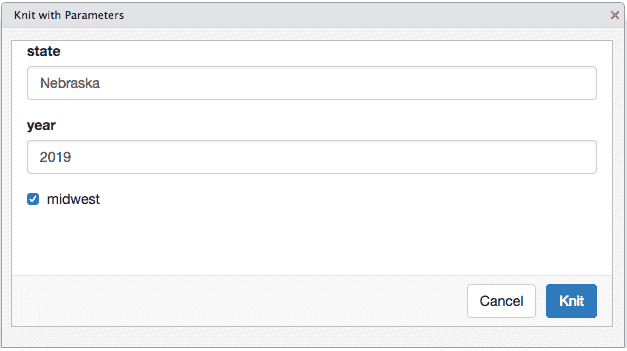
\includegraphics[width=1\linewidth,height=1\textheight,keepaspectratio]{JP/images/params-shiny} 

}

\caption{GUI から入力できるパラメータで R Markdown を knit する}\label{fig:params-shiny}
\end{figure}

パラメータ化されたレポートの詳細については, \emph{R Markdown Definitive Guide} \autocite{rmarkdown2018} の \href{https://bookdown.org/yihui/rmarkdown/parameterized-reports.html}{Chapter 15} を読むことができます.

\hypertarget{custom-knit}{%
\section{\texorpdfstring{\texttt{Knit} ボタンをカスタマイズする (*)}{Knit ボタンをカスタマイズする (*)}}\label{custom-knit}}

RStudio の \texttt{Knit} ボタン\index{RStudio!Knit button}をクリックする時, 新規の R セッション内で \texttt{rmarkdown::render()} が呼び出され, 同じディレクトリに入力ファイルと同じ基底名の出力ファイルが出力されます. 例えば出力フォーマット \texttt{html\_document} で \texttt{example.Rmd} を knit すると, \texttt{example.html} というファイルが作られます.

文書がどうレンダリングされるかをカスタマイズしたいという状況もあるでしょう. 例えば今日の日付を文書に含めたり, 別のディレクトリにコンパイルした文書を出力したいといったことがたぶんあるでしょう. こういったことは適切な \texttt{output\_file} 引数を付けた \texttt{rmarkdown::render()} を呼び出すことで達成可能 (\ref{rmarkdown-render}節参照) ですが, レポートをコンパイルするのに \texttt{rmarkdown::render()} を変更して呼び出すことに頼るのは不便という可能性があります.

文書の YAML フロントマターの \texttt{knit} フィールドを与えることで \texttt{Knit} ボタンの挙動を制御することが可能です. このフィールドは主要な引数 \texttt{input} を持つ関数を取ります. これは入力 Rmd 文書のパスです. 現時点では他の引数は無視されます. 関数のソースコードを直接 \texttt{knit} コードに書くことも, 他のどの場所でも, 例えば R パッケージの関数を与えて呼び出すことも可能です. カスタム \texttt{knit} 関数が日常的に必要ならば, 毎度のように R Markdown 文書に関数のソースコードを繰り返し書くのではなく, パッケージに関数を置くことをお薦めします.

YAML に直接ソースコードを置くなら, 関数全体をパーレン \texttt{()} で囲まなければなりません. ソースコードが複数行になるなら, 最初の行以外の全ての行にスペース2つ分のインデントをしなければなりません. 例えば出力ファイル名にレンダリングした日付を含めたい場合, 次のような YAML コードが使用可能です\index{YAML!knit}.

\begin{Shaded}
\begin{Highlighting}[]
\PreprocessorTok{{-}{-}{-}}
\FunctionTok{knit}\KeywordTok{:}\AttributeTok{ (function(input, ...) \{}
\AttributeTok{    rmarkdown::render(}
\AttributeTok{      input,}
\AttributeTok{      output\_file = paste0(}
\AttributeTok{        xfun::sans\_ext(input), \textquotesingle{}{-}\textquotesingle{}, Sys.Date(), \textquotesingle{}.html\textquotesingle{}}
\AttributeTok{      ),}
\AttributeTok{      envir = globalenv()}
\AttributeTok{    )}
\AttributeTok{  \})}
\PreprocessorTok{{-}{-}{-}}
\end{Highlighting}
\end{Shaded}

例えば 2019/07/29 に \texttt{example.Rmd} を knit したなら, 出力ファイル名は \texttt{example-2019-07-29.html} となります.

上記のアプローチは単純で十分に分かりやすいですが, 関数が R Markdown 文書で1度限りしか使われるのでない限り, YAML に直接関数を埋め込むのは管理を難しくさせるかもしれません そこで例えばパッケージ内に \texttt{knit\_with\_date()} という関数を作成することができます.

\begin{Shaded}
\begin{Highlighting}[numbers=left,,]
\CommentTok{\#\textquotesingle{} RStudio 用のカスタム knit 関数}
\CommentTok{\#\textquotesingle{}}
\CommentTok{\#\textquotesingle{} @export}
\NormalTok{knit\_with\_date }\OtherTok{\textless{}{-}} \ControlFlowTok{function}\NormalTok{(input, ...) \{}
\NormalTok{  rmarkdown}\SpecialCharTok{::}\FunctionTok{render}\NormalTok{(}
\NormalTok{    input,}
    \AttributeTok{output\_file =} \FunctionTok{paste0}\NormalTok{(}
\NormalTok{        xfun}\SpecialCharTok{::}\FunctionTok{sans\_ext}\NormalTok{(input), }\StringTok{\textquotesingle{}{-}\textquotesingle{}}\NormalTok{, }\FunctionTok{Sys.Date}\NormalTok{(), }\StringTok{\textquotesingle{}.\textquotesingle{}}\NormalTok{,}
\NormalTok{        xfun}\SpecialCharTok{::}\FunctionTok{file\_ext}\NormalTok{(input)}
\NormalTok{    ),}
    \AttributeTok{envir =} \FunctionTok{globalenv}\NormalTok{()}
\NormalTok{  )}
\NormalTok{\}}
\end{Highlighting}
\end{Shaded}

上記のコードを \textbf{myPackage} という名前のパッケージに追加すれば, 次のような YAML 設定を使いカスタム \texttt{knit} 関数を参照することが可能になります.

\begin{Shaded}
\begin{Highlighting}[]
\PreprocessorTok{{-}{-}{-}}
\FunctionTok{knit}\KeywordTok{:}\AttributeTok{ myPackage::knit\_with\_date}
\PreprocessorTok{{-}{-}{-}}
\end{Highlighting}
\end{Shaded}

\texttt{?rmarkdown::render} のヘルプページを見れば, \texttt{Knit} ボタンの背後にある \texttt{knit} 関数をどうカスタマイズするかのさらなるアイディアを見つけることもできるでしょう.

\hypertarget{google-drive}{%
\section{Google ドライブで Rmd 文書を共同編集する}\label{google-drive}}

\textbf{googledrive} パッケージ\index{R パッケージ!googledrive} \autocite{R-googledrive} を基にして, Emily Kothe は \textbf{rmdrive} パッケージ\index{R パッケージ!rmdrive} にいくつかのラッパ関数を提供しています. パッケージは現在 GitHub の \url{https://github.com/ekothe/rmdrive} から利用可能です. 文書を書いている時点では, リッチドキュメントが不足しています. そこで私は Janosch Linkersdörfer のフォークリポジトリ \url{https://github.com/januz/rmdrive} を代わりに推奨します. こちらは Ben Marwick のフォークに基づいています. もし GIT を学んだことがないなら, 自由にフォークし他人の GIT リポジトリを改善するこれらの事例によって学ぶ気になるかもしれません.

\textbf{rmdrive} のワークフローは大まかに言って以下のようになります.

\begin{enumerate}
\def\labelenumi{\arabic{enumi}.}
\item
  プロジェクトの主著者かコントリビュータがいて, その人は GIT のようなバージョン管理ツールを扱う能力があると仮定します. 主著者は Rmd 文書の初期版を書き, \texttt{upload\_rmd()} 関数で Google ドライブへアップグレードします.
\item
  Google ドライブの Rmd 文書は他の共同編集者たちと共有され, 編集者たちは Google ドキュメント上で変更をしたり改善提案をしたりできます.
\item
  主著者は提案された変更を受け容れたり, \texttt{render\_rmd()} 関数で Rmd 文書をローカルへダウンロード・プレビューしたりできます. 他の共同編集者たちもコードチャンクを修正し新たな結果を見たいならば, 自分で同様のことができます.
\item
  満足したら主著者は GIT リポジトリに変更をコミットできます.
\end{enumerate}

Google ドライブ上では共同編集作業を同期的に行うことも, 非同期的に行うことも可能です. 複数の人間が同じ文書を同時に編集することも, 先に他の人の編集が完了するまで待つことも可能です.

このパッケージには \texttt{update\_rmd()} 関数があり, Rmd 文書をローカルで編集して, このローカルな Rmd 文書を Google ドライブへアップロードすることが可能になります. これは Google ドライブ上の文書を完全に上書きしてしまうため, おそらくこの関数を実行すべきではないです. 主著者は予め共同編集者たちにこれを警告したいと思うでしょう. 全ての共同編集者たちが Google ドライブ上でのみ文書を編集し, ローカルでは編集すべきでない, というのが理想です. 編集された文書を \texttt{render\_rmd()} 関数でローカル上で閲覧するのは大丈夫ですが (\texttt{render\_rmd()} は文書をレンダリングする前に文書を自動的にダウンロードします).

\hypertarget{workflowr}{%
\section{\texorpdfstring{\textbf{workflowr} で R Markdown プロジェクトを研究用サイトでまとめる}{workflowr で R Markdown プロジェクトを研究用サイトでまとめる}}\label{workflowr}}

\textbf{workflowr} パッケージ\index{R パッケージ!workflowr} \autocite{R-workflowr,workflowr2019}は (データ分析の) プロジェクトをテンプレート\index{テンプレート!プロジェクト}とバージョン管理ツールである GIT を使って体系的に編成することが可能です. プロジェクトに変更を加えるたびに, 変更の記録を残すことが可能で, \textbf{workflowr} はプロジェクトの特定のバージョンと対応するウェブサイトを構築できます. これはあなたの分析結果の履歴をすべて閲覧することが可能になることを意味します. このパッケージはバージョン管理のためバックエンドで GIT を使用していますが, 特に GIT に詳しくなる必要はありません. このパッケージは, 内部で GIT の操作を行う R の関数を提供し, あなたはこれらの関数を呼び出す必要があるだけです. そのうえ, \textbf{workflowr} は自動的に再現可能なコードへのベストプラクティスを自動化します. R Markdown 文書がレンダリングされるたびに, \textbf{workflowr} は \texttt{set.seed()} でシード値を設定, \texttt{sessionInfo()} でセッション情報を記録, そして絶対ファイルパスをスキャンする, などなど, といったことを自動的に行います. このパッケージの導入方法と詳細は\href{https://jdblischak.github.io/workflowr/}{パッケージのドキュメント}をご覧ください.

\textbf{workflowr} の主著者である John Blischak は, R プロジェクトのワークフローと関連のあるパッケージとガイドを網羅的ではないですがリストにまとめています. これは GitHub レポジトリ \url{https://github.com/jdblischak/r-project-workflows} で見ることができます.

\hypertarget{blastula-email}{%
\section{R Markdown から Eメールを送信する Send emails based on R Markdown}\label{blastula-email}}

\textbf{blastula} パッケージ\index{R パッケージ!blastula}\index{email} \autocite{R-blastula}があれば Rmd 文書を Eメールの本文にして送信することが可能になります. Rmd 文書を Eメールへレンダリングするには, 文書に出力フォーマット \texttt{blastula::blastula\_email} を使用すること必要があります.

\begin{Shaded}
\begin{Highlighting}[]
\CommentTok{{-}{-}{-}}
\AnnotationTok{title:}\CommentTok{ 週次レポート}
\AnnotationTok{output:}\CommentTok{ blastula::blastula\_email}
\CommentTok{{-}{-}{-}} 

\NormalTok{ボスへ}

\NormalTok{お疲れ様です.}

\NormalTok{以下が }\InformationTok{\textasciigrave{}iris\textasciigrave{}}\NormalTok{ データの分析になります.}

\InformationTok{\textasciigrave{}\textasciigrave{}\textasciigrave{}\{r\}}
\InformationTok{summary(iris)}
\InformationTok{plot(iris[, {-}5])}
\InformationTok{\textasciigrave{}\textasciigrave{}\textasciigrave{}}

\NormalTok{もううんざりだというのなら知らせていただきたく.}

\NormalTok{よろしくお願いします}
\NormalTok{ジョン}
\end{Highlighting}
\end{Shaded}

この Rmd 文書は \texttt{blastula::render\_email()} 関数でレンダリングされるべきであり, 出力は \texttt{blastula::smtp\_send()} に渡すことができます. これはEメールを送信する関数です. \texttt{smtp\_send()} にはEメールサーバとあなたの認証が必要であることに注意してください.

RStudio Connect を使用しているなら, \url{https://solutions.rstudio.com/examples/blastula-overview/} で, 自動化したもの, 条件付けたもの, パラメータ化したEメールを含め, さらなる例を見ることができます.

\hypertarget{appendix-ux88dcux907a}{%
\appendix}


\hypertarget{full-options}{%
\chapter{\texorpdfstring{\textbf{knitr} のチャンク及びパッケージオプション}{knitr のチャンク及びパッケージオプション}}\label{full-options}}

\begin{rmdtip}
この付録は \url{https://gedevan-aleksizde.github.io/knitr-doc-ja/options.html} で公開されているものと同一です. \end{rmdtip}

\textbf{knitr} パッケージはソースコード, テキスト, グラフ, チャンクで使用するプログラミング言語といった, コードチャンクのコンポネントのほとんど全部をカスタマイズするための多くのオプションを提供します. \texttt{knit} 処理のカスタマイズをパッケージレベルでカスタマイズするオプションもあります. この章では \textbf{knitr} で使用できる全てのチャンクオプションとパッケージオプションを解説します. 以下のリスト中で, オプションのデフォルト値になっているものはカッコ内に表記しています.

\hypertarget{chunk-options-full}{%
\section{チャンクオプション一覧}\label{chunk-options-full}}

チャンクオプションはチャンクのヘッダに書きます. チャンクヘッダの構文は文書フォーマットがなんであるかに依存します. 例えば \texttt{.Rnw} ファイル (R + LaTeX) であれば, \texttt{\textless{}\textless{}\ \textgreater{}\textgreater{}=} という記号の中に書きます. \texttt{.Rmd} ならば, チャンクヘッダは \texttt{\textasciigrave{}\textasciigrave{}\textasciigrave{}\{r\}} 内に書きます. 以下の例は主に \texttt{.Rmd} (R Markdown) の場合ですが, ほとんどのチャンクオプションはどのフォーマットでも使用可能です.

チャンクオプションは以下のように \texttt{タグ名=値} という形式で書きます.

\begin{verbatim}
```{r, my-chunk, echo=FALSE, fig.height=4, dev='jpeg'}
```
\end{verbatim}

\textbf{チャンクラベル}は特殊なチャンクオプションです (例: 先ほどの例の \texttt{my-chunk} がそれにあたります). これは唯一のタグが不要なチャンクオプションです (つまり, 値のみ書くことになります). もし \texttt{タグ名=値} の形式で書きたいのならば, チャンクオプション名の \texttt{label} を明示的に使うこともできます.

\begin{verbatim}
```{r label="my-chunk"}
```
\end{verbatim}

各チャンクのラベルは文書内において一意であることが前提です. 特にキャッシュとグラフのファイル名はチャンクラベルで紐付けているため重要です. ラベルのないチャンクは \texttt{unnamed-chunk-i} という形式でラベル名が割り当てられます. \texttt{i} は順に整数が割り当てられます.

文書全体のチャンクオプションのデフォルト値を変更するために \texttt{knitr::opts\_chunk\$set()} を使うことができます. 例えば以下のようなチャンクを文書の冒頭に書きます.

\begin{verbatim}
```{r, setup, include=FALSE}
knitr::opts_chunk$set(
  comment = '', fig.width = 6, fig.height = 6
)
```
\end{verbatim}

チャンクオプションの豆知識をいくつか掲載します.

\begin{enumerate}
\def\labelenumi{\arabic{enumi}.}
\tightlist
\item
  チャンクヘッダは1行で書かねばなりません. 改行してはいけません.
\item
  チャンクラベルとファイルパスにスペース, ピリオド \texttt{.}, アンダースコア \texttt{\_} を使用するのは避けましょう. セパレータが必要ならば, ハイフン \texttt{-} の使用を推奨します. 例えば \texttt{setup-options} はラベル名として望ましいですが \texttt{setup.options} や \texttt{chunk 1} は良くありません. \texttt{fig.path = \textquotesingle{}figures/mcmc-\textquotesingle{}} はパス名として良いですが, \texttt{fig.path = \textquotesingle{}markov\ chain/monte\ carlo\textquotesingle{}} は良くありません.
\item
  全てのオプションの値は \textbf{R の構文として適切でなければなりません}. チャンクオプションを関数の引数のように考えると良いでしょう.
\end{enumerate}

\begin{itemize}
\tightlist
\item
  例えば \textbf{character} 型をとるオプションは引用符で囲まなければなりません. 例: \texttt{results = \textquotesingle{}asis\textquotesingle{}} や \texttt{out.width = \textquotesingle{}\textbackslash{}\textbackslash{}textwidth\textquotesingle{}}. ただしリテラルのバックスラッシュは二重のバックスラッシュが必要なことを忘れないでください.
\item
  理論上はチャンクラベルもまた引用符で囲む必要がありますが, 利便性のため書かなくとも自動で引用符が追加されます (例: \texttt{\textasciigrave{}\textasciigrave{}\textasciigrave{}\{r,\ 2a\}\textasciigrave{}\textasciigrave{}\textasciigrave{}} は \texttt{\textasciigrave{}\textasciigrave{}\textasciigrave{}\{r,\ label=\textquotesingle{}2a\textquotesingle{}\}\textasciigrave{}\textasciigrave{}\textasciigrave{}} として扱われます).
\item
  R のコードとして有効なものである限り, いくらでも複雑な構文を書くことができます.
\end{itemize}

以下では \texttt{オプション}: (\texttt{デフォルト値}; 値の型) という形式で, \textbf{knitr} で使えるチャンクオプションのリストを掲載します.

\hypertarget{evaluate}{%
\subsection{コード評価関連}\label{evaluate}}

\begin{itemize}
\tightlist
\item
  \textbf{\texttt{eval}}: (\texttt{TRUE}; \texttt{logical} または \texttt{numeric}).: コードチャンクを評価するかどうか. どの R の評価式を評価するかを選ぶために \texttt{numeric} のベクトルを使用することもできます. 例: \texttt{eval=c(1, 3, 4)} ならば1つ目, 3つ目, そして4つ目の評価式を評価し, \texttt{eval = -(4:5)} は 4, 5つ目の式以外の全てを評価します.
\end{itemize}

\hypertarget{text-output}{%
\subsection{テキストの出力関連}\label{text-output}}

\begin{itemize}
\tightlist
\item
  \textbf{\texttt{echo}}: (\texttt{TRUE}; \texttt{logical} または \texttt{numeric}).: 出力される文書にソースコードを表示するかどうか. 「表示」「隠す」に対応する \texttt{TRUE}/\texttt{FALSE} に加え, どの R の評価式を表示するかを選ぶために \texttt{numeric} のベクトルを使用することもできます. 例: \texttt{echo=2:3} は 2, 3番めの評価式を表示し, \texttt{echo = -4} は4番目だけを非表示にします.
\item
  \texttt{results}: (\texttt{\textquotesingle{}markup\textquotesingle{}}; \texttt{character}) 実行結果のテキストの部分をどう表示するかを制御します. このオプションは通常のテキスト出力にのみ影響することに注意してください (警告・メッセージ・エラーは適用範囲外です). 取りうる値は次のとおりです.

  \begin{itemize}
  \tightlist
  \item
    \texttt{markup}: 出力の文書フォーマットに応じて適切な環境でテキスト出力をマークアップします. 例えば R Markdown ならば \texttt{"{[}1{]}\ 1\ 2\ 3"} が \textbf{knitr} によって以下のように加工されます. この場合, \texttt{results=\textquotesingle{}markup\textquotesingle{}} は囲み (\texttt{\textasciigrave{}\textasciigrave{}\textasciigrave{}}) 付きのコードブロックとして出力されることを意味します.
  \end{itemize}

\begin{verbatim}
```
[1] 1 2 3
```
\end{verbatim}

  \begin{itemize}
  \tightlist
  \item
    \texttt{asis}: テキスト出力を「そのまま」書き出します. つまり, 生の結果テキストをマークアップ一切なしでそのまま文書に書き出します.
  \item
    \textbf{\texttt{hold}}: チャンクと flush の全てのテキスト出力をチャンクの末尾に固定します.
  \item
    \textbf{\texttt{hide}} (または \texttt{FALSE}): テキスト出力を表示しません.
  \end{itemize}
\item
  \texttt{collapse}: (\texttt{FALSE}; \texttt{logical}) 可能であれば, ソースと出力をつなげて1つのブロックにするかどうかです (デフォルトではソースと出力はそれぞれ独立したブロックです). このオプションは Markdown 文書でのみ有効です.
\item
  \textbf{\texttt{warning}}: (\texttt{TRUE}; \texttt{logical}).: 警告文 (\texttt{warning()} で出力されるテキスト) を保存するかどうかです. \texttt{FALSE} の場合, 全ての警告文は文書に出力されず, 代わりにコンソールに書き出されます. 警告文の一部を選ぶインデックスとして, \texttt{numeric} 型のベクトルを指定することもできます. この場合のインデックスの数値は「何番目の警告文を表示するか」を参照する (例: \texttt{3} はこのチャンクから投げられた3番目の警告文を意味します) ものであって, 「何番目の R コードの警告文の出力を許可するか」ではないことに注意してください.
\item
  \textbf{\texttt{error}}: (\texttt{TRUE}; \texttt{logical}).: エラー文 (\texttt{stop()} で出力される文です) を保持するかどうかです. デフォルトの \texttt{TRUE} では, \textbf{コード評価はエラーが出ても停止しません!} エラー時点で停止させたい場合はこのオプションを \texttt{FALSE} に指定してください. \textbf{R Markdown ではこのデフォルト値は \texttt{FALSE} に変更されていることに注意}してください. チャンクオプションに \texttt{include=FALSE} がある場合, 起こりうるエラーを見落とさないように, \textbf{knitr} はエラー時点で停止するようになります.
\item
  \textbf{\texttt{message}}: (\texttt{TRUE}; \texttt{logical}).: \texttt{message()} が出力するメッセージ文を (\texttt{warning} オプションと同様に) 表示するかどうかです.
\item
  \textbf{\texttt{include}}: (\texttt{TRUE}; \texttt{logical}).: 出力する文書にチャンクの出力を含めるかどうかです. \texttt{FALSE} ならばなにも書き出されませんが, コードの評価はなされ, チャンク内にプロット命令があるのならグラフのファイルも生成されます. よってこの図をそれ以降で任意に挿入することもできます.
\item
  \textbf{\texttt{strip.white}}: (\texttt{TRUE}; \texttt{logical}).: 出力時にソースコードの冒頭と末尾から空白行を除去するかどうかです.
\item
  \textbf{\texttt{class.output}}: (\texttt{NULL}; \texttt{character}).: テキストの出力ブロックに追加するクラス名のベクトル. このオプションは R Markdown で HTML を出力する際にのみ機能します. 例えば \texttt{class.output = c(\textquotesingle{}foo\textquotesingle{},\ \textquotesingle{}bar\textquotesingle{})} はテキスト出力が \texttt{\textless{}pre\ class="foo\ bar"\textgreater{}\textless{}/pre\textgreater{}} で囲まれたブロックとして書き出されます.
\item
  \textbf{\texttt{class.message}}/\textbf{\texttt{class.warning}}/\textbf{\texttt{class.error}}: (\texttt{NULL}; \texttt{character})・: \texttt{class.output} と同様に, R Markdown においてそれぞれ メッセージ文, 警告文, エラー文のブロックに対してクラス名を与えます. \texttt{class.source} もまた同様にソースコードのブロックに対して適用されます. \textcite{ref}(\#code-decoration)節を参照してください.
\item
  \textbf{\texttt{attr.output}}/\textbf{\texttt{attr.message}}/\textbf{\texttt{attr.warning}}/\textbf{\texttt{attr.error}}: (\texttt{NULL}; \texttt{character}).: 上記の \texttt{class.*} オプション群と同様に, Pandoc に対してコードブロックの属性を指定します. つまり \texttt{class.*} は \texttt{attr.*} の特殊ケースです. 例: \texttt{class.source = \textquotesingle{}numberLines\textquotesingle{}} は \texttt{attr.source = \textquotesingle{}.numberLines\textquotesingle{}} と等価ですが, \texttt{attr.source} は任意の値を取ることができます. 例えば, \texttt{attr.source = c(\textquotesingle{}.numberLines\textquotesingle{},\ \textquotesingle{}startFrom="11"\textquotesingle{})}.
\item
  \textbf{\texttt{render}}: (\texttt{knitr::knit\_print}; \texttt{function(x, options, ...)}).: チャンクで表示される値に対して適用する関数です. 関数の第1引数には (\texttt{x}) はチャンクの各評価式が評価された結果が与えられます. このチャンクのチャンクオプションがリストとして第二引数 \texttt{opstions} に与えられます. この関数は文字列を返すことを想定しています. 詳細は package vignette (\texttt{vignette(\textquotesingle{}knit\_print\textquotesingle{},\ package\ =\ \textquotesingle{}knitr\textquotesingle{})}) を参照してください.
\item
  \textbf{\texttt{split}}: (\texttt{FALSE}; \texttt{logical}).: 出力ブロックを分割したファイルに書き出すかどうか. LaTeX ならば \texttt{\textbackslash{}input\{\}} で読み込み, HTML ならば \texttt{\textless{}iframe\textgreater{}\textless{}/iframe\textgreater{}} タグで読み込まれます. このオプションは \texttt{.Rnw}, \texttt{.Rtex} そして \texttt{.Rhtml} でのみ機能します.
\end{itemize}

\hypertarget{code-decoration}{%
\subsection{コードの装飾関連}\label{code-decoration}}

\begin{itemize}
\tightlist
\item
  \texttt{tidy}: (\texttt{FALSE}) R コードを整形するかどうかです. 他の有効な値は次のとおりです.

  \begin{itemize}
  \tightlist
  \item
    \texttt{TRUE} (\texttt{tidy = \textquotesingle{}formatR\textquotesingle{}} と等価です): 整形のために \texttt{formatR::tidy\_source()} を呼び出します.
  \item
    \texttt{\textquotesingle{}styler\textquotesingle{}}: コード整形のために \texttt{styler::style\_text()} を呼び出します.
  \item
    整形されたコードを返す, \texttt{function(code, ...) \{\}} という形式の任意の関数.
  \item
    整形が失敗した場合, 元の R コードは変更されません (警告は表示されます).
  \end{itemize}
\item
  \texttt{tidy.opts}: (\texttt{NULL}; \texttt{list}) \texttt{tidy} オプションで指定した関数へのオプション引数のリストです. 例えば \texttt{tidy.opts = list(blank = FALSE, width.cutoff = 60)} は \texttt{tidy = \textquotesingle{}formatR\textquotesingle{}} に対して空白行を削除し各行が60文字におさまるように改行しようとします.
\item
  \texttt{prompt}: (\texttt{FALSE}; \texttt{logical}) R コードにプロンプト記号 (\texttt{\textgreater{}} など) を付けるかどうかです. \texttt{?base::options} ヘルプページの \texttt{prompt} と \texttt{continue} を参照してください. プロンプト記号の追加は, 読者がコードをコピーするのを難しくさせるため, \texttt{prompt=FALSE} のほうが良い選択であることに留意してください. エンジンが \texttt{R} 以外の場合, このオプションはうまく機能しないことがあります (issue \href{https://github.com/yihui/knitr/issues/1274}{\#1274}).
\item
  \textbf{\texttt{comment}}: (\texttt{\textquotesingle{}\#\#\textquotesingle{}}; \texttt{character}).: テキスト出力の各行の先頭文字です. デフォルトでは, コメントアウトできるよう \texttt{\#\#} となっているので, 読者は文書から任意の範囲をそのままコピーしても出力部分は無視されるのでそのまま実行することができます. \texttt{comment = \textquotesingle{}\textquotesingle{}} を指定することで, デフォルトの \texttt{\#\#} は除去されます.
\item
  \textbf{\texttt{highlight}}: (\texttt{TRUE}; \texttt{logical}).: ソースコードをシンタックスハイライトするかどうかです\footnote{訳注: R Markdown ではさらに, YAML フロントマターで適用するハイライトのテーマ名を指定できます}.
\item
  \textbf{\texttt{class.source}}: (\texttt{NULL}; \texttt{character}).: 出力された文書のソースコードブロックのクラス名です. 出力ブロックに対して機能する \texttt{class.output} をはじめとする \texttt{class.*} シリーズと同様です.
\item
  \textbf{\texttt{attr.source}}: (\texttt{NULL}; \texttt{character}).: ソースコードブロックの属性です. \texttt{attr.output} などの \texttt{attr.*} シリーズと同様です.
\item
  \texttt{size}: (\texttt{\textquotesingle{}normalsize\textquotesingle{}}; \texttt{character}) \texttt{.Rnw} 使用時のチャンクサイズのフォントサイズです. 指定可能なサイズは \href{https://www.overleaf.com/learn/latex/Font_sizes,_families,_and_styles}{overleaf のヘルプページ (英語)} を参照してください\footnote{訳注: \texttt{\textbackslash{}normalsize}, \texttt{\textbackslash{}Large}, \texttt{\textbackslash{}LARGE} など LaTeX で指定できるフォントサイズを表すマクロのことを指しています}.
\item
  \textbf{\texttt{background}}: (\texttt{\textquotesingle{}\#F7F7F7\textquotesingle{}}; \texttt{character}).: \texttt{.Rnw} 使用時のチャンクブロックの背景色です\footnote{訳注: R Markdown では背景色は CSS や \texttt{class.output} などで設定する必要があります. 詳細は R Markdown Cookbook などを参照してください}.
\item
  \textbf{\texttt{indent}}: (\texttt{character}).: チャンクの出力で各行に追加する文字です. 典型的には空白と同義です. このオプションは読み込み専用を想定しており, 値は \textbf{knitr} が文書を読み込む際に設定されます. 例えば以下のチャンクでは, \texttt{indent} は空白文字2個です\footnote{訳注: R Markdown の場合は \textbf{knitr} 以外の中間処理があるため, 必ずしもこのルールを守りません}.
\end{itemize}

\begin{Shaded}
\begin{Highlighting}[numbers=left,,]
\FunctionTok{rnorm}\NormalTok{(}\DecValTok{10}\NormalTok{)}
\end{Highlighting}
\end{Shaded}

\begin{verbatim}
##  [1]  1.37096 -0.56470  0.36313  0.63286  0.40427
##  [6] -0.10612  1.51152 -0.09466  2.01842 -0.06271
\end{verbatim}

\hypertarget{cache-options}{%
\subsection{キャッシュ関連}\label{cache-options}}

\begin{itemize}
\tightlist
\item
  \textbf{\texttt{cache}}: (\texttt{FALSE}; \texttt{logical}).: コードチャンクのキャッシュを取るかどうかです. 初回の実行またはキャッシュが存在しない場合は通常通り実行され, 結果がデータセットが保存され (\texttt{.rdb}, \texttt{.rdx} ファイルなど), それ以降でコードチャンクが評価されることがあれば, 以前保存されたこれらのファイルからこのチャンクの結果を読み出します. ファイル名がチャンクラベルと R コードの MD5 ハッシュ値で一致する必要があることに注意してください. つまりチャンクになんらかの変更がある度に異なる MD5 ハッシュ値が生成されるため, キャッシュはその度に無効になります. 詳細は \href{https://gedevan-aleksizde.github.io/knitr-doc-ja/cache.html\#cache}{キャッシュの解説} を参考にしてください.
\item
  \textbf{\texttt{cache.path}}: (\texttt{\textquotesingle{}cache/\textquotesingle{}}; \texttt{character}).: 生成したキャッシュファイルの保存場所を指定します. R Markdown ではデフォルトでは入力ファイルの名前に基づきます. 例えば \texttt{INPUT.Rmd} の \texttt{FOO} というラベルのチャンクのキャッシュは \texttt{INPUT\_cache/FOO\_*.*} というファイルパスに保存されます.
\item
  \textbf{\texttt{cache.vars}}: (\texttt{NULL}; \texttt{character}).: キャッシュデータベースに保存される変数名のベクトルを指定します. デフォルトではチャンクで作られた全ての変数が識別され保存されますが, 変数名の自動検出はロバストではないかもしれませんし, 保存したい変数を選別したい場合もあるかもしれないので, 保存したい変数を手動選択することもできます.
\item
  \textbf{\texttt{cache.globals}}: (\texttt{NULL}; \texttt{character}).: このチャンクで作成されない変数の名前のベクトルを指定します. このオプションは主に \texttt{autodep = TRUE} オプションをより正確に動作させたいときに使います. チャンク \texttt{B} で使われているグローバル変数が チャンク \texttt{A} のローカル変数として使われているときなど. グローバル変数の自動検出に失敗した際に使う場合, こにオプションを使って手動でグローバル変数の名前を指定してください (具体例として issue \href{https://github.com/yihui/knitr/issues/1403}{\#1403} を参照してください).
\item
  \textbf{\texttt{cache.lazy}}: (\texttt{TRUE}; logical).: 遅延読み込み \texttt{lazyLoad()} を使うか, 直接 \texttt{load()} でオブジェクトを読み込むかを指定します. 非常に大きなオブジェクトに対しては, 遅延読み込みは機能しないかもしれません. よってこの場合は \texttt{cache.lazy = FALSE} が望ましいかもしれません (issue \href{https://github.com/yihui/knitr/issues/572}{\#572} を参照してください).
\item
  \textbf{\texttt{cache.comments}}: (\texttt{NULL}; \texttt{logical}).: \texttt{FALSE} の場合, R コードチャンク内のコメントを書き換えてもキャッシュが無効になりません.
\item
  \textbf{\texttt{cache.rebuild}}: (\texttt{FALSE}; \texttt{logical}).: \texttt{TRUE} の場合, キャッシュが有効であってもチャンクのコードの再評価を行います. このオプションはキャッシュの無効化の条件を指定したいときに有用です. 例えば \texttt{cache.rebuild = !file.exists("some-file")} とすれば \texttt{some-file} が存在しないときにチャンクが評価されキャッシュが再構成されます (issue \href{https://github.com/yihui/knitr/issues/238}{\#238} を参照).
\item
  \textbf{\texttt{dependson}}: (\texttt{NULL}; \texttt{character} または \texttt{numeric}).: このチャンクが依存しているチャンクのラベル名を文字ベクトルで指定します. このオプションはキャッシュされたチャンクでのみ適用されます. キャッシュされたチャンク内のオブジェクトは, 他のキャッシュされたチャンクに依存しているかもしれず, 他のチャンクの変更に合わせてこのチャンクも更新する必要があるかもしれません.
\item
  \texttt{dependson} に \texttt{numeric} ベクトルを与えた場合, それはチャンクラベルのインデックスを意味します. 例えば \texttt{dependson = 1} ならばこの文書の1番目のチャンクに依存することを意味し, \texttt{dependson = c(-1, -2)} は直前の2つのチャンクを意味します (負のインデックスは現在のチャンクからの相対的な位置を表します).
\item
  \texttt{opts\_chunk\$set()} によってグローバルにチャンクオプションを設定した場合, このオプションは機能しません. ローカルなチャンクオプションとして設定しなければなりません.
\item
  \textbf{\texttt{autodep}}: (\texttt{FALSE}; \texttt{logical}).: グローバル変数を検出することでチャンク間の依存関係を分析するかどうかを指定します (あまり信頼できません). よって, \texttt{dependson} を明示的に指定する必要はありません.
\end{itemize}

\hypertarget{plots}{%
\subsection{グラフ関連}\label{plots}}

\begin{itemize}
\tightlist
\item
  \textbf{\texttt{fig.path}}: (\texttt{\textquotesingle{}figure/\textquotesingle{}}; \texttt{character}).: 図の保存ファイルパスを生成する際の接尾語. \texttt{fig.path} とチャンクラベルを連結したものがフルパスになります. \texttt{figure/prefix-} のようにディレクトリ名が含まれて, それが存在しない場合はディレクトリが作成されます.
\item
  \textbf{\texttt{fig.keep}}: (\texttt{\textquotesingle{}high\textquotesingle{}}; \texttt{character}).: グラフをどのように保存するかです. 可能な値は次のとおりです.

  \begin{itemize}
  \tightlist
  \item
    \texttt{high}: 高水準プロットのみ保存 (低水準の変更は全て高水準プロットに統合されます).
  \item
    \texttt{none}: 全て破棄します.
  \item
    \texttt{all}: 全てのプロットを保存します (低水準プロットでの変更は新しいグラフとして保存されます).
  \item
    \texttt{first}: 最初のプロットのみ保存します.
  \item
    \texttt{last}: 最後のプロットのみ保存します.
  \item
    数値ベクトルを指定した場合, その値は保存する低水準プロットのインデックスとなります. 低水準プロットとは \texttt{lines()} や \texttt{points()} などの関数によるグラフ描画のことです. \texttt{fig.keep} についてより理解するには次のようなチャンクを考えてください. 通常はこれで2つのグラフを出力します (\texttt{fig.keep = \textquotesingle{}high\textquotesingle{}} を指定したので). \texttt{fig.keep = \textquotesingle{}none\textquotesingle{}} としたなら, いかなるグラフも保存されません. \texttt{fig.keep = \textquotesingle{}all\textquotesingle{}} ならば, 4 つのグラフとして保存されます. \texttt{fig.keep = \textquotesingle{}first\textquotesingle{}} ならば \texttt{plot(1)} によって作成されたグラフが保存されます. \texttt{fig.keep = \textquotesingle{}last\textquotesingle{}}, なら, 最後の10本の垂線を描画したグラフが保存されます.
  \end{itemize}
\end{itemize}

\begin{Shaded}
\begin{Highlighting}[numbers=left,,]
\FunctionTok{plot}\NormalTok{(}\DecValTok{1}\NormalTok{)  }\CommentTok{\# 高水準プロット}
\FunctionTok{abline}\NormalTok{(}\DecValTok{0}\NormalTok{, }\DecValTok{1}\NormalTok{)  }\CommentTok{\# 低水準の作図}
\FunctionTok{plot}\NormalTok{(}\FunctionTok{rnorm}\NormalTok{(}\DecValTok{10}\NormalTok{))  }\CommentTok{\# 高水準プロット}
\CommentTok{\# ループ内での複数の低水準作図 (R 評価式としては1つ)}
\ControlFlowTok{for}\NormalTok{ (i }\ControlFlowTok{in} \DecValTok{1}\SpecialCharTok{:}\DecValTok{10}\NormalTok{) \{}
  \FunctionTok{abline}\NormalTok{(}\AttributeTok{v =}\NormalTok{ i, }\AttributeTok{lty =} \DecValTok{2}\NormalTok{)}
\NormalTok{\}}
\end{Highlighting}
\end{Shaded}

\begin{itemize}
\tightlist
\item
  \textbf{\texttt{fig.show}}: (\texttt{\textquotesingle{}asis\textquotesingle{}}; \texttt{character}).: グラフをどのように表示し, 配置するかです. 可能な値は次のとおりです.

  \begin{itemize}
  \tightlist
  \item
    \texttt{asis}: グラフが生成された場所にそのまま出力します (R ターミナルで実行した場合とおなじように).
  \item
    \texttt{hold}: 全てのグラフをまとめてチャンクの最後に出力します.
  \item
    \texttt{animate}: チャンクに複数のグラフがある場合, 連結して1つのアニメーションにします.
  \item
    \texttt{hide}: グラフをファイルに保存しますが, 出力時は隠します.
  \end{itemize}
\item
  \textbf{\texttt{dev}}: (LaTeX の場合は \texttt{\textquotesingle{}pdf\textquotesingle{}}\footnote{訳注: \texttt{pdf} は日本語表示に向いていないため, \texttt{cairo\_pdf} などを利用することをおすすめします}, HTML/Markdown の場合は \texttt{\textquotesingle{}png\textquotesingle{}}; \texttt{character}).: グラフをファイルに保存する際のグラフィックデバイスです. base R および, \textbf{\texttt{Cairo}}, \textbf{\texttt{cairoDevice}}, \textbf{\texttt{svglite}}, \textbf{\texttt{ragg}}, \textbf{tikzDevice} パッケージの提供するデバイスに対応しています. デバイスの例: \texttt{pdf}, \texttt{png}, \texttt{svg}, \texttt{jpeg}, \texttt{tiff}, \texttt{cairo\_pdf}, \texttt{CairoJPEG}, \texttt{CairoPNG}, \texttt{Cairo\_pdf}, \texttt{Cairo\_png}, \texttt{svglite}, \texttt{ragg\_png}, \texttt{tikz}, など. 有効なデバイスの一覧は \texttt{names(knitr:::auto\_exts)} を参照してください. また, \texttt{function(filename, width, height)} という引数を定義した関数名を文字列で与えることでも指定できます. 画像サイズの単位は \textbf{常にインチ}です. ビットマップであってもインチで指定したものがピクセルに変換されます.
\end{itemize}

チャンクオプション \texttt{dev}, \texttt{fig.ext}, \texttt{fig.width}, \texttt{fig.height}, \texttt{dpi} はベクトルを与えられます (長さが足りない場合は再利用されます). 例えば \texttt{dev = c(\textquotesingle{}pdf\textquotesingle{},\ \textquotesingle{}png\textquotesingle{})} は1つのグラフに対して 1つづつ \texttt{PDF} と \texttt{PNG} ファイルを作成します.

\begin{itemize}
\tightlist
\item
  \textbf{\texttt{dev.args}}: (\texttt{NULL}; \texttt{list}).: グラフィックデバイスに与える追加の引数です. 例えば \texttt{dev.args = list(bg = \textquotesingle{}yellow\textquotesingle{},\ pointsize\ =\ 10)} を \texttt{dev = \textquotesingle{}png\textquotesingle{}} に与えられます. 特定のデバイスに依存するオプション (詳細はそれぞれのデバイスのドキュメントを確認してくだささい). \texttt{dev} に複数のデバイスが指定されている場合は \texttt{dev.args} を引数のリストをさらにリストでくくることになるでしょう. それぞれの引数リストが対応するデバイスに与えられます. 例: \texttt{dev = c(\textquotesingle{}pdf\textquotesingle{},\ \textquotesingle{}tiff\textquotesingle{}),\ dev.args\ =\ list(pdf\ =\ list(colormodel\ =\ \textquotesingle{}cmyk\textquotesingle{},\ useDingats\ =\ TRUE),\ tiff\ =\ list(compression\ =\ \textquotesingle{}lzw\textquotesingle{}))}.
\item
  \textbf{\texttt{fig.ext}}: (\texttt{NULL}; \texttt{character}).: 出力するグラフのファイル拡張子です. \texttt{NULL} ならばグラフィックデバイスに応じて自動決定されます. 詳細は \texttt{knitr:::auto\_exts} を確認してください.
\item
  \textbf{\texttt{dpi}}: (\texttt{72}; \texttt{numeric}). ビットマップデバイスに対する DPI (インチ毎ドット, \texttt{dpi * inches = pixels}) です.
\item
  \textbf{\texttt{fig.width}}, \textbf{\texttt{fig.height}}: (いずれも \texttt{7}; \texttt{numeric}).: グラフの幅と高さです. 単位はインチです. グラフィックデバイスに与えられます.
\item
  \textbf{\texttt{fig.asp}}: (\texttt{NULL}; \texttt{numeric}).: グラフのアスペクト比, つまり 高さ/幅 の比です. \texttt{fig.asp} が指定された場合, 高さ (\texttt{fig.height}) は \texttt{fig.width * fig.asp} によって自動設定されます.
\item
  \textbf{\texttt{fig.dim}}: (\texttt{NULL}; \texttt{numeric}).: \texttt{fig.width} と \texttt{fig.height} を指定する長さ2の数値のベクトルです. 例: \texttt{fig.dim = c(5, 7)} は \texttt{fig.width = 5, fig.height = 7} の省略形です. \texttt{fig.asp} と \texttt{fig.dim} が指定された場合, \texttt{fig.asp} は無視されます (警告文が出力されます).
\item
  \textbf{\texttt{out.width}}, \textbf{\texttt{out.height}}: (\texttt{NULL}; \texttt{character}).: 出力時の画像の幅と高さです. 実体としての幅と高さである \texttt{fig.width} と \texttt{fig.height} とは異なります. つまりグラフは文書に表示される際にスケールが調整されます. 出力フォーマットに応じて, これら2つのオプションはそれぞれ特殊な値を取ることができます. 例えば LaTeX ならば \texttt{.8\textbackslash{}\textbackslash{}linewidth}, \texttt{3in}, \texttt{8cm} などと指定でき, HTML ならば \texttt{300px} と指定できます. \texttt{.Rnw} ならば \texttt{out.width} のデフォルト値は \texttt{\textbackslash{}\textbackslash{}maxwidth} に変更され, その値は \href{https://gedevan-aleksizde.github.io/knitr-doc-ja/framed.html\#framed}{framed のページ} で書いたように定義されます. 例えば \texttt{\textquotesingle{}40\%\textquotesingle{}} のようにパーセンテージで指定もでき, これは LaTeX では \texttt{0.4\textbackslash{}linewidth} に置き換えられます.
\item
  \textbf{\texttt{out.extra}}: (\texttt{NULL}; \texttt{character}).: 図の表示に関するその他のオプションです. LaTeX で出力する場合は \texttt{\textbackslash{}includegraphics{[}{]}} に挿入される任意の文字に対応し (例: \texttt{out.extra = \textquotesingle{}angle=90\textquotesingle{}} ならば図の90度回転), HTML なら \texttt{\textless{}img\ /\textgreater{}} に挿入されます (例: \texttt{out.extra = \textquotesingle{}style="border:5px\ solid\ orange;"\textquotesingle{}}).
\item
  \textbf{\texttt{fig.retina}}: (\texttt{1}; \texttt{numeric}).: このオプションは HTML で出力する際にのみ適用されます. \href{https://ja.wikipedia.org/wiki/Retina\%E3\%83\%87\%E3\%82\%A3\%E3\%82\%B9\%E3\%83\%97\%E3\%83\%AC\%E3\%82\%A4}{Retina ディスプレイ} に対して画像サイズを調整する比率 (多くの場合は2を指定します) です. チャンクオプションの \texttt{dpi} を \texttt{dpi * fig.retina} で, \texttt{out.width} を \texttt{fig.width * dpi / fig.retina} で計算します. 例えば \texttt{fig.retina = 2} なら, 画像の物理サイズが2倍となり, その表示サイズは半分になります.
\item
  \textbf{\texttt{resize.width}}, \textbf{\texttt{resize.height}}: (\texttt{NULL}; \texttt{character}).: LaTeX で出力する際に \texttt{\textbackslash{}resizebox\{\}\{\}} コマンドで使われます. これら2つのオプションは Tikz グラフィックスをリサイズしたい場合のみ必要になります. それ以外に通常使うことはありません. しかし \textbf{tikzDevice} の開発者によれば, 他の箇所のテキストとの一貫性のため, Tikz グラフィックスはリサイズを想定していません. 値の1つでも \texttt{NULL} ならば, \texttt{!} が使用されます (この意味がわからない方は \textbf{graphicx} のドキュメントを読んでください).
\item
  \textbf{\texttt{fig.align}}: (\texttt{\textquotesingle{}default\textquotesingle{}}; \texttt{character}).: 出力時の画像の位置揃え (アラインメント) です. 可能な値は \texttt{default}, \texttt{left}, \texttt{right}, \texttt{center} です. \texttt{default} は位置について特に何も調整しません.
\item
  \textbf{\texttt{fig.link}}: (\texttt{NULL}; \texttt{character}) 画像に与えるリンク.
\item
  \textbf{\texttt{fig.env}}: (\texttt{\textquotesingle{}figure\textquotesingle{}}; \texttt{character}).: 画像に使われる LaTeX 環境. 例えば \texttt{fig.env = \textquotesingle{}marginfigure\textquotesingle{}} ならば \texttt{\textbackslash{}begin\{marginfigure\}} で囲まれます. このオプションの使用は \texttt{fig.cap} が指定されいることが条件です.
\item
  \textbf{\texttt{fig.cap}}: (\texttt{NULL}; \texttt{character}).: 図のキャプションです.
\item
  \textbf{\texttt{fig.alt}}: (\texttt{NULL}; \texttt{character}) HTML 出力時の図の \texttt{\textless{}img\textgreater{}} タグの \texttt{alt} 属性に使う代替テキストです. デフォルトでは, 代替テキストが与えられた場合チャンクオプション \texttt{fig.cap} には代替テキストが使われます.
\item
  \textbf{\texttt{fig.scap}}: (\texttt{NULL}; \texttt{character}).: 図の短縮キャプションです. 出力が LaTeX の場合のみ意味をなします. 短縮キャプションは \texttt{\textbackslash{}caption{[}{]}} コマンドに挿入され, 大抵の場合は PDF 出力時の「図一覧」で表示される見出しとして使われます.
\item
  \textbf{\texttt{fig.lp}}: (\texttt{\textquotesingle{}fig:\textquotesingle{}}; \texttt{character}).; 図の相互参照に使われるラベル\footnote{訳注: チャンクラベルと混同しないでください}の接頭語で, \texttt{\textbackslash{}label\{\}} コマンドに挿入されます. 実際のラベルはこの接頭語とチャンクラベルを連結して作られます. 例えば図のラベルが \texttt{\textasciigrave{}\textasciigrave{}\textasciigrave{}\{r,\ foo-plot\}} will be ならば, デフォルトでは図のラベルは \texttt{fig:foo-plot} になります.
\item
  \textbf{\texttt{fig.pos}}: (\texttt{\textquotesingle{}\textquotesingle{}}; \texttt{character}).: LaTeX の \texttt{\textbackslash{}begin\{figure\}{[}{]}} に使われる, 画像の位置調整オプション\footnote{訳注: LaTeX では通常は図の位置は調整されますが, \texttt{fig.pos=\textquotesingle{}H\textquotesingle{}} ならばその位置で固定されます}を指定します.
\item
  \textbf{\texttt{fig.subcap}}: (\texttt{NULL}).: subfigures のためのキャプションです. 複数のグラフが1つのチャンクにあり, かつ \texttt{fig.subcap} も \texttt{fig.cap} is \texttt{NULL} である場合, \texttt{\textbackslash{}subfloat\{\}} が個別の画像の表示に使われます (この場合はプリアンブルに \texttt{\textbackslash{}usepackage\{subfig\}} と書く必要があります). 具体例は \href{https://github.com/yihui/knitr-examples/blob/master/067-graphics-options.Rnw}{067-graphics-options.Rnw} を参照してください.
\item
  \textbf{\texttt{fig.ncol}}: (\texttt{NULL}; \texttt{integer}). subfigure の数です. 例えば\href{https://github.com/yihui/knitr/issues/1327\#issuecomment-346242532}{この issue} を見てください (\texttt{fig.ncol} も \texttt{fig.sep} も LaTeX でのみ機能します).
\item
  \textbf{\texttt{fig.sep}}: (\texttt{NULL}; \texttt{character}).: subfigures どうしの間に挿入されるセパレータを指定する文字ベクトルです. \texttt{fig.ncol} が指定された場合, デフォルトでは \texttt{fig.sep} に N 個ごとに \texttt{\textbackslash{}newline} が挿入されます (\texttt{N} は列の数です). 例えば \texttt{fig.ncol = 2} ならばデフォルトは \texttt{fig.sep = c(\textquotesingle{}\textquotesingle{},\ \textquotesingle{}\textquotesingle{},\ \textquotesingle{}\textbackslash{}\textbackslash{}newline\textquotesingle{},\ \textquotesingle{}\textquotesingle{},\ \textquotesingle{}\textquotesingle{},\ \textquotesingle{}\textbackslash{}\textbackslash{}newline\textquotesingle{},\ \textquotesingle{}\textquotesingle{},\ ...)} となります.
\item
  \textbf{\texttt{fig.process}}: (\texttt{NULL}; \texttt{function}).: 画像ファイルに対する後処理の関数です. 関数は画像のファイルパスを引数として, 挿入したい新しい画像のファイルを返すものであるべきです. 関数に \texttt{options} 引数がある場合, この引数にチャンクオプションのリストが与えられます.
\item
  \textbf{\texttt{fig.showtext}}: (\texttt{NULL}; \texttt{logical}).: \texttt{TRUE} ならばグラフの描画前に \texttt{showtext::showtext\_begin()} が呼ばれます. 詳細は \href{http://cran.rstudio.com/package=showtext}{\textbf{\texttt{showtext}}} パッケージのドキュメントを参照してください\footnote{訳注: \texttt{showtext} は手っ取り早く日本語を表示できますが, いくつかの制約があります. 詳細は『\href{https://ill-identified.hatenablog.com/entry/2020/10/03/200618}{おまえはもうRのグラフの日本語表示に悩まない (各OS対応)}』『\href{https://oku.edu.mie-u.ac.jp/~okumura/stat/font.html}{Rでのフォントの扱い}』などを見てください.}.
\item
  \textbf{\texttt{external}}: (\texttt{TRUE}; \texttt{logical}).: tikz グラフィックの処理 (PDF 生成時のコンパイル前の処理) を外部化するかどうかです. \textbf{tikzDevice} パッケージの \texttt{tikz()} デバイスを使う場合 (つまり \texttt{dev=\textquotesingle{}tikz\textquotesingle{}} を指定したとき) のみ使用され, コンパイル時間を短縮することが可能です.
\item
  \textbf{\texttt{sanitize}}: (\texttt{FALSE}; \texttt{character}). tikz グラフィックでサニタイズ (ここでは, LaTeXで特殊な意味を持つ文字のエスケープ処理) するかどうかです. 詳細は \textbf{tikzDevice} パッケージのドキュメントを参照してください.
\end{itemize}

さらにこの他に, ユーザーが使用することを想定していない隠しオプションが2つあります. \texttt{fig.cur} (複数の図表がある場合の, 現在の図番号/インデックス) と \texttt{fig.num} (チャンク内の図の合計数) です. これら2つのオプションは \textbf{knitr} が複数の図そしてアニメーションを処理するためにあります. 場合によっては手動で保存した画像ファイルを使ってアニメーションを書き出す場合などに役に立つかもしれません (使用例として \href{https://github.com/yihui/knitr/releases/download/doc/knitr-graphics.pdf}{graphics manual} を参照してください).

\hypertarget{animation-options}{%
\subsection{アニメーション関連}\label{animation-options}}

\begin{itemize}
\tightlist
\item
  \textbf{\texttt{interval}}: (\texttt{1}; \texttt{numeric}).: アニメーションの1フレームごとの時間 (単位は秒) です.
\item
  \textbf{\texttt{animation.hook}}: (\texttt{knitr::hook\_ffmpeg\_html}; \texttt{function} または \texttt{character}). HTML 出力時のアニメーション作成用のフック関数を指定します. デフォルトでは FFmpeg を使って WebM 動画ファイルに変換します.

  \begin{itemize}
  \tightlist
  \item
    別のフック関数として \href{https://cran.r-project.org/package=gifski}{\textbf{gifski}} パッケージの \texttt{knitr::hook\_gifski} 関数はGIFアニメーションを作ることができます.
  \item
    このオプションは \texttt{\textquotesingle{}ffmpeg\textquotesingle{}} や \texttt{\textquotesingle{}gifski\textquotesingle{}} といった文字列を指定することもできます. これらは対応するフック関数の省略形です. 例: \texttt{animation.hook = \textquotesingle{}gifski\textquotesingle{}} は \texttt{animation.hook = knitr::hook\_gifski} を意味します.
  \end{itemize}
\item
  \textbf{\texttt{aniopts}}: (\texttt{\textquotesingle{}controls,loop\textquotesingle{}}; \texttt{character}).: アニメーションに対する追加のオプションです. 詳細は LaTeX の \href{http://ctan.org/pkg/animate}{\textbf{animate} パッケージのドキュメント}を参照してください.
\item
  \textbf{\texttt{ffmpeg.bitrate}}: (\texttt{1M}; \texttt{character}).: WebM 動画の質を制御するための FFmpeg の引数 \texttt{-b:v} に対応する値を指定できます.
\item
  \textbf{\texttt{ffmpeg.format}}: (\texttt{webm}; \texttt{character}).: FFmpeg の出力する動画フォーマットです. つまり, 動画ファイルの拡張子名です.
\end{itemize}

\hypertarget{code-chunk}{%
\subsection{コードチャンク関連}\label{code-chunk}}

\begin{itemize}
\tightlist
\item
  \textbf{\texttt{code}}: (\texttt{NULL}; \texttt{character}).: 指定された場合, そのチャンクのコードを上書きします. この機能によって, プログラミング的にコード挿入が可能になります. 例えば \texttt{code = readLines(\textquotesingle{}test.R\textquotesingle{})} とすれば \texttt{test.R} の内容を現在のチャンクで実行します.
\item
  \textbf{\texttt{ref.label}}: (\texttt{NULL}; \texttt{character}).: 現在のチャンクのコードに引き継ぐ, 別のチャンクのラベルの文字列ベクトルを指定します (動作例は \href{https://gedevan-aleksizde.github.io/knitr-doc-ja/reference.html\#reference}{チャンク参照} を確認してください).
\end{itemize}

\hypertarget{child-document-appendix}{%
\subsection{子文書関連}\label{child-document-appendix}}

\begin{itemize}
\tightlist
\item
  \textbf{\texttt{child}}: (\texttt{NULL}; \texttt{character}).: 親文書に挿入する子文書のファイルパスを示す文字ベクトルを指定します.
\end{itemize}

\hypertarget{engine}{%
\subsection{言語エンジン関連}\label{engine}}

\begin{itemize}
\tightlist
\item
  \textbf{\texttt{engine}}: (\texttt{\textquotesingle{}R\textquotesingle{}}; \texttt{character}).: コードチャンクの言語名です. 指定可能な名前は \texttt{names(knitr::knit\_engines\$get())} で確認できます. 例: \texttt{python}, \texttt{sql}, \texttt{julia}, \texttt{bash}, \texttt{c}, など. \texttt{knitr::knit\_engines} で他の言語を使うためのセットアップが可能です.
\item
  \textbf{\texttt{engine.path}}: (\texttt{NULL}; \texttt{character}).: 実行可能なエンジンのパスを指定します. あなたのお使いのシステムの別の実行ファイルを使用するためのオプションです. 例えば \texttt{python} はデフォルトでは \texttt{/usr/bin/python} を参照しますが, 他のバージョンを使うため \texttt{engine.path = \textquotesingle{}\textasciitilde{}/anaconda/bin/python\textquotesingle{}} などと指定することもできます\footnote{訳注: R Markdown の場合, Python のバージョンは \texttt{reticulate} パッケージでも制御できます. むしろそちらをつかったほうが便利だと思われます.}. \texttt{engine.path} もまたパスのリストを与えられます. これによってエンジンごとにそれぞれパスを指定することができます. 以下のコードが例です. リストの名前はエンジン名と一致する必要があります.
\end{itemize}

\begin{Shaded}
\begin{Highlighting}[numbers=left,,]
\NormalTok{knitr}\SpecialCharTok{::}\NormalTok{opts\_chunk}\SpecialCharTok{$}\FunctionTok{set}\NormalTok{(}\AttributeTok{engine.path =} \FunctionTok{list}\NormalTok{(}\AttributeTok{python =} \StringTok{"\textasciitilde{}/anaconda/bin/python"}\NormalTok{, }
  \AttributeTok{ruby =} \StringTok{"/usr/local/bin/ruby"}\NormalTok{))}
\end{Highlighting}
\end{Shaded}

\hypertarget{ux30aaux30d7ux30b7ux30e7ux30f3ux30c6ux30f3ux30d7ux30ecux30fcux30c8ux95a2ux9023}{%
\subsection{オプションテンプレート関連}\label{ux30aaux30d7ux30b7ux30e7ux30f3ux30c6ux30f3ux30d7ux30ecux30fcux30c8ux95a2ux9023}}

\begin{itemize}
\tightlist
\item
  \textbf{\texttt{opts.label}}: (\texttt{NULL}; \texttt{character}).: \texttt{knitr::opts\_template} でのオプションのラベルです. オプションセットのラベルは \texttt{knitr::opts\_template} で設定できます (\texttt{?knitr::opts\_template} を参照してください). このオプションにより, 頻繁に使うチャンクオプションのタイピング労力を削減できます.
\end{itemize}

\textbf{訳注}: 例えば次のように, \texttt{echo=F} を設定するテンプレート \texttt{noecho} をどこかで作成したとします. すると, 以降のチャンクで \texttt{opts.label="noecho"} を設定すると \texttt{opts\_template} で設定した \texttt{noecho} のオプションが全て適用されます. もちろん複数のオプションをまとめることもできるので, 定番の設定を使いまわすのが簡単になります.

\begin{Shaded}
\begin{Highlighting}[numbers=left,,]
\NormalTok{knitr}\SpecialCharTok{::}\NormalTok{opts\_template}\SpecialCharTok{$}\FunctionTok{set}\NormalTok{(}\AttributeTok{noecho =} \FunctionTok{list}\NormalTok{(}\AttributeTok{echo =}\NormalTok{ F))}
\end{Highlighting}
\end{Shaded}

\hypertarget{ux30bdux30fcux30b9ux30b3ux30fcux30c9ux306eux62bdux51faux95a2ux9023}{%
\subsection{ソースコードの抽出関連}\label{ux30bdux30fcux30b9ux30b3ux30fcux30c9ux306eux62bdux51faux95a2ux9023}}

\begin{itemize}
\tightlist
\item
  \textbf{\texttt{purl}}: (\texttt{TRUE}; \texttt{logical}).: ソースドキュメントから \texttt{knitr::purl()} でソースコードを取りだす時, このチャンクを含めるか除外するかどうかです.
\end{itemize}

\hypertarget{ux305dux306eux4ed6ux306eux30c1ux30e3ux30f3ux30afux30aaux30d7ux30b7ux30e7ux30f3}{%
\subsection{その他のチャンクオプション}\label{ux305dux306eux4ed6ux306eux30c1ux30e3ux30f3ux30afux30aaux30d7ux30b7ux30e7ux30f3}}

\begin{itemize}
\tightlist
\item
  \textbf{\texttt{R.options}}: (\texttt{NULL}; \texttt{list}).: コードチャンク内でのローカルな R オプションを指定します. これらは \texttt{options()} によってこのコードチャンクの直前に一時的に設定され, 実行後に戻されます.
\end{itemize}

\hypertarget{package-options}{%
\section{パッケージオプション一覧}\label{package-options}}

パッケージオプションは \href{https://gedevan-aleksizde.github.io/knitr-doc-ja/objects.html\#objects}{\texttt{knitr::opts\_knit}} を使用することで変更できます. \textbf{\texttt{knitr::opts\_chunk} と混同しないでください}. 使用例は以下のとおりです.

\begin{Shaded}
\begin{Highlighting}[numbers=left,,]
\NormalTok{knitr}\SpecialCharTok{::}\NormalTok{opts\_knit}\SpecialCharTok{$}\FunctionTok{set}\NormalTok{(}\AttributeTok{progress =} \ConstantTok{TRUE}\NormalTok{, }\AttributeTok{verbose =} \ConstantTok{TRUE}\NormalTok{)}
\end{Highlighting}
\end{Shaded}

別の方法として, R の基本関数である \texttt{options()} を使ってパッケージオプションを設定する場合は \texttt{?knitr::opts\_knit} を参照してください.

可能なオプションは次のとおりです.

\begin{itemize}
\tightlist
\item
  \textbf{\texttt{aliases}}: (\texttt{NULL}; \texttt{character}).: チャンクオプションのエイリアスを指定する名前付きベクトルです. 例えば \texttt{c(h = \textquotesingle{}fig.height\textquotesingle{},\ w\ =\ \textquotesingle{}fig.width\textquotesingle{})} は \textbf{knitr} に \texttt{h} は \texttt{fig.height} \texttt{w} は \texttt{fig.width} と同じ意味だと認識させます. このオプションは名前の長いチャンクオプションのタイピング労力を削減できます.
\item
  \textbf{\texttt{base.dir}}: (\texttt{NULL}; \texttt{character}).: グラフを生成する際のディレクトリの絶対パスです.
\item
  \textbf{\texttt{base.url}}: (\texttt{NULL}; \texttt{character}).: HTML ページに掲載する画像のベースURLです.
\item
  \textbf{\texttt{concordance}}: (\texttt{FALSE}; \texttt{logical}).: この機能は RStudio によって実装されている機能で, \texttt{.Rnw} でのみ有効です. 入力ファイルの行番号に対応した行番号を出力ファイルに書き出すかどうかを指定します. これにより, 出力から入力の誘導が可能になり, 特に LaTeX のエラー発生時に役に立ちます.
\item
  \textbf{\texttt{eval.after}}: (\texttt{c(\textquotesingle{}fig.cap\textquotesingle{},\ \textquotesingle{}fig.alt\textquotesingle{};}character\texttt{).: オプション名の文字ベクトルを指定します. このオプションはチャンクが評価された**後で**評価され, 他の全てのオプションはチャンクが評価される前に評価されます. 例えば}eval.after = `fig.cap'\texttt{が指定されているときに}fig.cap = paste(`p-value is', t.test(x)\$p.value)\texttt{とすると,}eval.after\texttt{にはチャンクの評価後の}x` の値が使用されます.
\item
  \textbf{\texttt{global.par}}: (\texttt{FALSE}; \texttt{logical}).: \texttt{TRUE} にすると, それ以前のコードチャンクでの \texttt{par()} での設定が引き継がれます (もちろん, この設定は R グラフィックスのみで有効です). デフォルトでは \textbf{knitr} はグラフの記録のために新規のグラフィックデバイスを開き, コードの評価後に閉じるため, \texttt{par()} による設定はその都度破棄されます.
\item
  \textbf{\texttt{header}}: (\texttt{NULL}; \texttt{character}).: 文書の開始前に挿入するテキストを指定します. (例えば, LaTeX ならば \texttt{\textbackslash{}documentclass\{article\}} の直後, HTML ならば \texttt{\textless{}head\textgreater{}} タグの直後). このオプションは LaTeX プリアンブルや HTML ヘッダでコマンドやスタイルの定義をするのに有用です. ドキュメントの開始地点は \texttt{knitr::knit\_patterns\$get(\textquotesingle{}document.begin\textquotesingle{})} で知ることができます. このオプションは \texttt{.Rnw} と \texttt{.Rhtml} 限定の機能です\footnote{訳注: R Markdown ではヘッダの設定は YAML フロントマターで行います}.
\item
  \texttt{label.prefix}: (\texttt{c(table = \textquotesingle{}tab:\textquotesingle{})}; character) ラベルの接頭語を指定します. 現時点では \texttt{kable::kable()} によって生成される表のラベルに対する接頭語のみサポートしています.
\item
  \textbf{\texttt{latex.options.color}}, \textbf{\texttt{latex.options.graphicx}}: (\texttt{NULL}).: それぞれ LaTeX パッケージの \textbf{color} と \textbf{graphicx} に対するオプションを指定します. これらのオプションは \texttt{.Rnw} 限定の機能です\footnote{訳注: R Markdown ではこの機能もやはり YAML フロントマターが担当しています}.
\item
  \textbf{\texttt{out.format}}: (\texttt{NULL}; \texttt{character}).: 可能な値は \texttt{latex}, \texttt{sweave}, \texttt{html}, \texttt{markdown}, \texttt{jekyll} です. このオプションは入力ファイル名に応じて自動で決定され, 自動設定されるフック関数に影響します. 例えば \texttt{?knitr::render\_latex} を参考にしてください. このオプションは \texttt{knitr::knit()} が実行される\textbf{前に}設定する必要があります (文書内で設定しても機能しません).
\item
  \textbf{\texttt{progress}}: (\texttt{TRUE}; \texttt{logical}).: \texttt{knitr::knit()} の実行中にプログレスバーを表示するかどうかを指定します.
\item
  \textbf{\texttt{root.dir}}: (\texttt{NULL}; \texttt{character}).: コードチャンク評価時のルートディレクトリを指定します. \texttt{NULL} の場合, 入力ファイルと同じ場所が指定されます.
\item
  \textbf{\texttt{self.contained}}: (\texttt{TRUE}; \texttt{logical}).: 出力する文書が自己完結的であるべきかどうかを指定します (\texttt{.tex} ファイルにスタイルを書き出すか, \texttt{html} に CSS を書き出すか). このオプションは \texttt{.Rnw} と \texttt{.Rhtml} でのみ機能します\footnote{訳注: R Markdown では出力フォーマット関数に同様のオプションが用意されていることが多いです}.
\item
  \textbf{\texttt{unnamed.chunk.label}}: (\texttt{unnamed-chunk}; \texttt{character}).: ラベルを設定していないチャンクのラベルの接頭語を指定します.
\item
  \textbf{\texttt{upload.fun}}: (\texttt{identity}; \texttt{function}).: ファイルパスを引数にとり, ファイルに対して処理を行い出力フォーマットが HTML または Markdown の場合に文字列を返す関数を指定します. 典型的な使い方として, 画像をアップロードしそのリンクを返す関数を指定します. 例えば \texttt{knitr::opts\_knit\$set(upload.fun = knitr::imgur\_upload)} でファイルを \url{http://imgur.com} にアップロードできます (\texttt{?knitr::imgur\_upload} を参照してください).
\item
  \textbf{\texttt{verbose}}: (\texttt{FALSE}; \texttt{logical}).: 情報を冗長に詳細するか (例えば各チャンクで実行されたRコードやメッセージログなど), チャンクラベルとオプションのみ表示するかを指定します.
\end{itemize}

\backmatter


% --- bibliography settings ---

% biblatex mode
\printbibliography[title=参考文献,heading=bibintoc]
% --- bibliography settings ends ---


\printindex

\end{document}
